\documentclass[twoside]{book}

% Packages required by doxygen
\usepackage{calc}
\usepackage{doxygen}
\usepackage{graphicx}
\usepackage[utf8]{inputenc}
\usepackage{makeidx}
\usepackage{multicol}
\usepackage{multirow}
\usepackage{textcomp}
\usepackage[table]{xcolor}

% Font selection
\usepackage[T1]{fontenc}
\usepackage{mathptmx}
\usepackage[scaled=.90]{helvet}
\usepackage{courier}
\usepackage{amssymb}
\usepackage{sectsty}
\renewcommand{\familydefault}{\sfdefault}
\allsectionsfont{%
  \fontseries{bc}\selectfont%
  \color{darkgray}%
}
\renewcommand{\DoxyLabelFont}{%
  \fontseries{bc}\selectfont%
  \color{darkgray}%
}

% Page & text layout
\usepackage{geometry}
\geometry{%
  a4paper,%
  top=2.5cm,%
  bottom=2.5cm,%
  left=2.5cm,%
  right=2.5cm%
}
\tolerance=750
\hfuzz=15pt
\hbadness=750
\setlength{\emergencystretch}{15pt}
\setlength{\parindent}{0cm}
\setlength{\parskip}{0.2cm}
\makeatletter
\renewcommand{\paragraph}{%
  \@startsection{paragraph}{4}{0ex}{-1.0ex}{1.0ex}{%
    \normalfont\normalsize\bfseries\SS@parafont%
  }%
}
\renewcommand{\subparagraph}{%
  \@startsection{subparagraph}{5}{0ex}{-1.0ex}{1.0ex}{%
    \normalfont\normalsize\bfseries\SS@subparafont%
  }%
}
\makeatother

% Headers & footers
\usepackage{fancyhdr}
\pagestyle{fancyplain}
\fancyhead[LE]{\fancyplain{}{\bfseries\thepage}}
\fancyhead[CE]{\fancyplain{}{}}
\fancyhead[RE]{\fancyplain{}{\bfseries\leftmark}}
\fancyhead[LO]{\fancyplain{}{\bfseries\rightmark}}
\fancyhead[CO]{\fancyplain{}{}}
\fancyhead[RO]{\fancyplain{}{\bfseries\thepage}}
\fancyfoot[LE]{\fancyplain{}{}}
\fancyfoot[CE]{\fancyplain{}{}}
\fancyfoot[RE]{\fancyplain{}{\bfseries\scriptsize Generated on Thu Mar 14 2019 15\-:51\-:38 for pymtt by Doxygen }}
\fancyfoot[LO]{\fancyplain{}{\bfseries\scriptsize Generated on Thu Mar 14 2019 15\-:51\-:38 for pymtt by Doxygen }}
\fancyfoot[CO]{\fancyplain{}{}}
\fancyfoot[RO]{\fancyplain{}{}}
\renewcommand{\footrulewidth}{0.4pt}
\renewcommand{\chaptermark}[1]{%
  \markboth{#1}{}%
}
\renewcommand{\sectionmark}[1]{%
  \markright{\thesection\ #1}%
}

% Indices & bibliography
\usepackage{natbib}
\usepackage[titles]{tocloft}
\setcounter{tocdepth}{3}
\setcounter{secnumdepth}{5}
\makeindex

% Hyperlinks (required, but should be loaded last)
\usepackage{ifpdf}
\ifpdf
  \usepackage[pdftex,pagebackref=true]{hyperref}
\else
  \usepackage[ps2pdf,pagebackref=true]{hyperref}
\fi
\hypersetup{%
  colorlinks=true,%
  linkcolor=blue,%
  citecolor=blue,%
  unicode%
}

% Custom commands
\newcommand{\clearemptydoublepage}{%
  \newpage{\pagestyle{empty}\cleardoublepage}%
}


%===== C O N T E N T S =====

\begin{document}

% Titlepage & ToC
\hypersetup{pageanchor=false}
\pagenumbering{roman}
\begin{titlepage}
\vspace*{7cm}
\begin{center}%
{\Large pymtt }\\
\vspace*{1cm}
{\large Generated by Doxygen 1.8.6}\\
\vspace*{0.5cm}
{\small Thu Mar 14 2019 15:51:38}\\
\end{center}
\end{titlepage}
\clearemptydoublepage
\tableofcontents
\clearemptydoublepage
\pagenumbering{arabic}
\hypersetup{pageanchor=true}

%--- Begin generated contents ---
\chapter{Main Page}
\label{index}\hypertarget{index}{}See \hyperlink{group___stages}{Stages} for details on the stages of test execution.\par
 See \hyperlink{group___tools}{Tools} for details on the plugins required by Stages.\par
 See \hyperlink{group___utilities}{Utilities} for details on the plugins used by the M\-T\-T framework.\par

\chapter{Module Index}
\section{Modules}
Here is a list of all modules\-:\begin{DoxyCompactList}
\item \contentsline{section}{Stages}{\pageref{group___stages}}{}
\begin{DoxyCompactList}
\item \contentsline{section}{B\-I\-O\-S}{\pageref{group___b_i_o_s}}{}
\item \contentsline{section}{Firmware}{\pageref{group___firmware}}{}
\item \contentsline{section}{Launcher\-Defaults}{\pageref{group___launcher_defaults}}{}
\item \contentsline{section}{Middleware\-Build}{\pageref{group___middleware_build}}{}
\item \contentsline{section}{Middleware\-Get}{\pageref{group___middleware_get}}{}
\item \contentsline{section}{M\-T\-T\-Defaults}{\pageref{group___m_t_t_defaults}}{}
\item \contentsline{section}{Profile}{\pageref{group___profile}}{}
\item \contentsline{section}{Provision}{\pageref{group___provision}}{}
\item \contentsline{section}{Reporter}{\pageref{group___reporter}}{}
\item \contentsline{section}{Test\-Build}{\pageref{group___test_build}}{}
\item \contentsline{section}{Test\-Get}{\pageref{group___test_get}}{}
\item \contentsline{section}{Test\-Run}{\pageref{group___test_run}}{}
\end{DoxyCompactList}
\item \contentsline{section}{Tools}{\pageref{group___tools}}{}
\begin{DoxyCompactList}
\item \contentsline{section}{Build}{\pageref{group___build}}{}
\item \contentsline{section}{C\-N\-C}{\pageref{group___c_n_c}}{}
\item \contentsline{section}{Executor}{\pageref{group___executor}}{}
\item \contentsline{section}{Fetch}{\pageref{group___fetch}}{}
\item \contentsline{section}{Harasser}{\pageref{group___harasser}}{}
\item \contentsline{section}{Launcher}{\pageref{group___launcher}}{}
\item \contentsline{section}{Version}{\pageref{group___version}}{}
\end{DoxyCompactList}
\item \contentsline{section}{Utilities}{\pageref{group___utilities}}{}
\end{DoxyCompactList}

\chapter{Namespace Index}
\section{Packages}
Here are the packages with brief descriptions (if available)\-:\begin{DoxyCompactList}
\item\contentsline{section}{\hyperlink{namespace_a_l_p_s}{A\-L\-P\-S} }{\pageref{namespace_a_l_p_s}}{}
\item\contentsline{section}{\hyperlink{namespace_already_installed}{Already\-Installed} }{\pageref{namespace_already_installed}}{}
\item\contentsline{section}{\hyperlink{namespace_autotools}{Autotools} }{\pageref{namespace_autotools}}{}
\item\contentsline{section}{\hyperlink{namespace_base_m_t_t_utility}{Base\-M\-T\-T\-Utility} }{\pageref{namespace_base_m_t_t_utility}}{}
\item\contentsline{section}{\hyperlink{namespace_b_i_o_s_m_t_t_stage}{B\-I\-O\-S\-M\-T\-T\-Stage} }{\pageref{namespace_b_i_o_s_m_t_t_stage}}{}
\item\contentsline{section}{\hyperlink{namespace_build_m_t_t_tool}{Build\-M\-T\-T\-Tool} }{\pageref{namespace_build_m_t_t_tool}}{}
\item\contentsline{section}{\hyperlink{namespace_check_profile}{Check\-Profile} }{\pageref{namespace_check_profile}}{}
\item\contentsline{section}{\hyperlink{namespace_c_n_c_m_t_t_tool}{C\-N\-C\-M\-T\-T\-Tool} }{\pageref{namespace_c_n_c_m_t_t_tool}}{}
\item\contentsline{section}{\hyperlink{namespacecombinatorial}{combinatorial} }{\pageref{namespacecombinatorial}}{}
\item\contentsline{section}{\hyperlink{namespace_compilers}{Compilers} }{\pageref{namespace_compilers}}{}
\item\contentsline{section}{\hyperlink{namespace_copy}{Copy} }{\pageref{namespace_copy}}{}
\item\contentsline{section}{\hyperlink{namespace_copytree}{Copytree} }{\pageref{namespace_copytree}}{}
\item\contentsline{section}{\hyperlink{namespace_default_m_t_t_defaults}{Default\-M\-T\-T\-Defaults} }{\pageref{namespace_default_m_t_t_defaults}}{}
\item\contentsline{section}{\hyperlink{namespace_default_profile}{Default\-Profile} }{\pageref{namespace_default_profile}}{}
\item\contentsline{section}{\hyperlink{namespace_default_test_build}{Default\-Test\-Build} }{\pageref{namespace_default_test_build}}{}
\item\contentsline{section}{\hyperlink{namespace_environ}{Environ} }{\pageref{namespace_environ}}{}
\item\contentsline{section}{\hyperlink{namespace_execute_cmd}{Execute\-Cmd} }{\pageref{namespace_execute_cmd}}{}
\item\contentsline{section}{\hyperlink{namespace_executor_m_t_t_tool}{Executor\-M\-T\-T\-Tool} }{\pageref{namespace_executor_m_t_t_tool}}{}
\item\contentsline{section}{\hyperlink{namespace_fetch_m_t_t_tool}{Fetch\-M\-T\-T\-Tool} }{\pageref{namespace_fetch_m_t_t_tool}}{}
\item\contentsline{section}{\hyperlink{namespace_firmware_m_t_t_stage}{Firmware\-M\-T\-T\-Stage} }{\pageref{namespace_firmware_m_t_t_stage}}{}
\item\contentsline{section}{\hyperlink{namespace_foo_flash}{Foo\-Flash} }{\pageref{namespace_foo_flash}}{}
\item\contentsline{section}{\hyperlink{namespace_git}{Git} }{\pageref{namespace_git}}{}
\item\contentsline{section}{\hyperlink{namespace_harasser}{Harasser} }{\pageref{namespace_harasser}}{}
\item\contentsline{section}{\hyperlink{namespace_harasser_m_t_t_tool}{Harasser\-M\-T\-T\-Tool} }{\pageref{namespace_harasser_m_t_t_tool}}{}
\item\contentsline{section}{\hyperlink{namespace_hostfile}{Hostfile} }{\pageref{namespace_hostfile}}{}
\item\contentsline{section}{\hyperlink{namespace_i_p_m_i_tool}{I\-P\-M\-I\-Tool} }{\pageref{namespace_i_p_m_i_tool}}{}
\item\contentsline{section}{\hyperlink{namespace_i_u_database}{I\-U\-Database} }{\pageref{namespace_i_u_database}}{}
\item\contentsline{section}{\hyperlink{namespace_junit_x_m_l}{Junit\-X\-M\-L} }{\pageref{namespace_junit_x_m_l}}{}
\item\contentsline{section}{\hyperlink{namespace_launcher_defaults_m_t_t_stage}{Launcher\-Defaults\-M\-T\-T\-Stage} }{\pageref{namespace_launcher_defaults_m_t_t_stage}}{}
\item\contentsline{section}{\hyperlink{namespace_launcher_m_t_t_tool}{Launcher\-M\-T\-T\-Tool} }{\pageref{namespace_launcher_m_t_t_tool}}{}
\item\contentsline{section}{\hyperlink{namespace_load_classes}{Load\-Classes} }{\pageref{namespace_load_classes}}{}
\item\contentsline{section}{\hyperlink{namespace_logger}{Logger} }{\pageref{namespace_logger}}{}
\item\contentsline{section}{\hyperlink{namespace_middleware_build_m_t_t_stage}{Middleware\-Build\-M\-T\-T\-Stage} }{\pageref{namespace_middleware_build_m_t_t_stage}}{}
\item\contentsline{section}{\hyperlink{namespace_middleware_get_m_t_t_stage}{Middleware\-Get\-M\-T\-T\-Stage} }{\pageref{namespace_middleware_get_m_t_t_stage}}{}
\item\contentsline{section}{\hyperlink{namespace_module_cmd}{Module\-Cmd} }{\pageref{namespace_module_cmd}}{}
\item\contentsline{section}{\hyperlink{namespace_m_p_i_version}{M\-P\-I\-Version} }{\pageref{namespace_m_p_i_version}}{}
\item\contentsline{section}{\hyperlink{namespace_m_t_t_defaults_m_t_t_stage}{M\-T\-T\-Defaults\-M\-T\-T\-Stage} }{\pageref{namespace_m_t_t_defaults_m_t_t_stage}}{}
\item\contentsline{section}{\hyperlink{namespace_m_t_t_version_plugin}{M\-T\-T\-Version\-Plugin} }{\pageref{namespace_m_t_t_version_plugin}}{}
\item\contentsline{section}{\hyperlink{namespace_o_m_p_i___snapshot}{O\-M\-P\-I\-\_\-\-Snapshot} }{\pageref{namespace_o_m_p_i___snapshot}}{}
\item\contentsline{section}{\hyperlink{namespace_open_m_p_i}{Open\-M\-P\-I} }{\pageref{namespace_open_m_p_i}}{}
\item\contentsline{section}{\hyperlink{namespace_profile_m_t_t_stage}{Profile\-M\-T\-T\-Stage} }{\pageref{namespace_profile_m_t_t_stage}}{}
\item\contentsline{section}{\hyperlink{namespace_provision_m_t_t_stage}{Provision\-M\-T\-T\-Stage} }{\pageref{namespace_provision_m_t_t_stage}}{}
\item\contentsline{section}{\hyperlink{namespacepymtt}{pymtt} }{\pageref{namespacepymtt}}{}
\item\contentsline{section}{\hyperlink{namespace_reporter_m_t_t_stage}{Reporter\-M\-T\-T\-Stage} }{\pageref{namespace_reporter_m_t_t_stage}}{}
\item\contentsline{section}{\hyperlink{namespacesequential}{sequential} }{\pageref{namespacesequential}}{}
\item\contentsline{section}{\hyperlink{namespace_shell}{Shell} }{\pageref{namespace_shell}}{}
\item\contentsline{section}{\hyperlink{namespace_s_l_u_r_m}{S\-L\-U\-R\-M} }{\pageref{namespace_s_l_u_r_m}}{}
\item\contentsline{section}{\hyperlink{namespacetest___test_def}{test\-\_\-\-Test\-Def} }{\pageref{namespacetest___test_def}}{}
\item\contentsline{section}{\hyperlink{namespace_test_build_m_t_t_stage}{Test\-Build\-M\-T\-T\-Stage} }{\pageref{namespace_test_build_m_t_t_stage}}{}
\item\contentsline{section}{\hyperlink{namespace_test_def}{Test\-Def} }{\pageref{namespace_test_def}}{}
\item\contentsline{section}{\hyperlink{namespace_test_get_m_t_t_stage}{Test\-Get\-M\-T\-T\-Stage} }{\pageref{namespace_test_get_m_t_t_stage}}{}
\item\contentsline{section}{\hyperlink{namespace_test_run_m_t_t_stage}{Test\-Run\-M\-T\-T\-Stage} }{\pageref{namespace_test_run_m_t_t_stage}}{}
\item\contentsline{section}{\hyperlink{namespace_text_file}{Text\-File} }{\pageref{namespace_text_file}}{}
\item\contentsline{section}{\hyperlink{namespace_version_m_t_t_tool}{Version\-M\-T\-T\-Tool} }{\pageref{namespace_version_m_t_t_tool}}{}
\item\contentsline{section}{\hyperlink{namespace_watchdog}{Watchdog} }{\pageref{namespace_watchdog}}{}
\item\contentsline{section}{\hyperlink{namespace_w_wulf3}{W\-Wulf3} }{\pageref{namespace_w_wulf3}}{}
\end{DoxyCompactList}

\chapter{Hierarchical Index}
\section{Class Hierarchy}
This inheritance list is sorted roughly, but not completely, alphabetically\-:\begin{DoxyCompactList}
\item Thread\begin{DoxyCompactList}
\item \contentsline{section}{I\-P\-M\-I\-Tool.\-worker\-Thread}{\pageref{class_i_p_m_i_tool_1_1worker_thread}}{}
\end{DoxyCompactList}
\item I\-Plugin\begin{DoxyCompactList}
\item \contentsline{section}{Base\-M\-T\-T\-Utility.\-Base\-M\-T\-T\-Utility}{\pageref{class_base_m_t_t_utility_1_1_base_m_t_t_utility}}{}
\begin{DoxyCompactList}
\item \contentsline{section}{Compilers.\-Compilers}{\pageref{class_compilers_1_1_compilers}}{}
\item \contentsline{section}{Copy.\-Copy}{\pageref{class_copy_1_1_copy}}{}
\item \contentsline{section}{Copytree.\-Copytree}{\pageref{class_copytree_1_1_copytree}}{}
\item \contentsline{section}{Environ.\-Environ}{\pageref{class_environ_1_1_environ}}{}
\item \contentsline{section}{Execute\-Cmd.\-Execute\-Cmd}{\pageref{class_execute_cmd_1_1_execute_cmd}}{}
\item \contentsline{section}{Logger.\-Logger}{\pageref{class_logger_1_1_logger}}{}
\item \contentsline{section}{Module\-Cmd.\-Module\-Cmd}{\pageref{class_module_cmd_1_1_module_cmd}}{}
\item \contentsline{section}{M\-P\-I\-Version.\-M\-P\-I\-Version}{\pageref{class_m_p_i_version_1_1_m_p_i_version}}{}
\item \contentsline{section}{Watchdog.\-Watchdog}{\pageref{class_watchdog_1_1_watchdog}}{}
\end{DoxyCompactList}
\item \contentsline{section}{B\-I\-O\-S\-M\-T\-T\-Stage.\-B\-I\-O\-S\-M\-T\-T\-Stage}{\pageref{class_b_i_o_s_m_t_t_stage_1_1_b_i_o_s_m_t_t_stage}}{}
\item \contentsline{section}{Build\-M\-T\-T\-Tool.\-Build\-M\-T\-T\-Tool}{\pageref{class_build_m_t_t_tool_1_1_build_m_t_t_tool}}{}
\begin{DoxyCompactList}
\item \contentsline{section}{Autotools.\-Autotools}{\pageref{class_autotools_1_1_autotools}}{}
\item \contentsline{section}{Hostfile.\-Hostfile}{\pageref{class_hostfile_1_1_hostfile}}{}
\item \contentsline{section}{Shell.\-Shell}{\pageref{class_shell_1_1_shell}}{}
\end{DoxyCompactList}
\item \contentsline{section}{C\-N\-C\-M\-T\-T\-Tool.\-C\-N\-C\-M\-T\-T\-Tool}{\pageref{class_c_n_c_m_t_t_tool_1_1_c_n_c_m_t_t_tool}}{}
\begin{DoxyCompactList}
\item \contentsline{section}{I\-P\-M\-I\-Tool.\-I\-P\-M\-I\-Tool}{\pageref{class_i_p_m_i_tool_1_1_i_p_m_i_tool}}{}
\end{DoxyCompactList}
\item \contentsline{section}{Executor\-M\-T\-T\-Tool.\-Executor\-M\-T\-T\-Tool}{\pageref{class_executor_m_t_t_tool_1_1_executor_m_t_t_tool}}{}
\begin{DoxyCompactList}
\item \contentsline{section}{combinatorial.\-Combinatorial\-Ex}{\pageref{classcombinatorial_1_1_combinatorial_ex}}{}
\item \contentsline{section}{sequential.\-Sequential\-Ex}{\pageref{classsequential_1_1_sequential_ex}}{}
\end{DoxyCompactList}
\item \contentsline{section}{Fetch\-M\-T\-T\-Tool.\-Fetch\-M\-T\-T\-Tool}{\pageref{class_fetch_m_t_t_tool_1_1_fetch_m_t_t_tool}}{}
\begin{DoxyCompactList}
\item \contentsline{section}{Already\-Installed.\-Already\-Installed}{\pageref{class_already_installed_1_1_already_installed}}{}
\item \contentsline{section}{Git.\-Git}{\pageref{class_git_1_1_git}}{}
\item \contentsline{section}{O\-M\-P\-I\-\_\-\-Snapshot.\-O\-M\-P\-I\-\_\-\-Snapshot}{\pageref{class_o_m_p_i___snapshot_1_1_o_m_p_i___snapshot}}{}
\end{DoxyCompactList}
\item \contentsline{section}{Firmware\-M\-T\-T\-Stage.\-Firmware\-M\-T\-T\-Stage}{\pageref{class_firmware_m_t_t_stage_1_1_firmware_m_t_t_stage}}{}
\begin{DoxyCompactList}
\item \contentsline{section}{Foo\-Flash.\-Foo\-Flash}{\pageref{class_foo_flash_1_1_foo_flash}}{}
\end{DoxyCompactList}
\item \contentsline{section}{Harasser\-M\-T\-T\-Tool.\-Harasser\-M\-T\-T\-Tool}{\pageref{class_harasser_m_t_t_tool_1_1_harasser_m_t_t_tool}}{}
\begin{DoxyCompactList}
\item \contentsline{section}{Harasser.\-Harasser}{\pageref{class_harasser_1_1_harasser}}{}
\end{DoxyCompactList}
\item \contentsline{section}{Launcher\-Defaults\-M\-T\-T\-Stage.\-Launcher\-Defaults\-M\-T\-T\-Stage}{\pageref{class_launcher_defaults_m_t_t_stage_1_1_launcher_defaults_m_t_t_stage}}{}
\item \contentsline{section}{Launcher\-M\-T\-T\-Tool.\-Launcher\-M\-T\-T\-Tool}{\pageref{class_launcher_m_t_t_tool_1_1_launcher_m_t_t_tool}}{}
\begin{DoxyCompactList}
\item \contentsline{section}{A\-L\-P\-S.\-A\-L\-P\-S}{\pageref{class_a_l_p_s_1_1_a_l_p_s}}{}
\item \contentsline{section}{Open\-M\-P\-I.\-Open\-M\-P\-I}{\pageref{class_open_m_p_i_1_1_open_m_p_i}}{}
\item \contentsline{section}{S\-L\-U\-R\-M.\-S\-L\-U\-R\-M}{\pageref{class_s_l_u_r_m_1_1_s_l_u_r_m}}{}
\end{DoxyCompactList}
\item \contentsline{section}{Middleware\-Build\-M\-T\-T\-Stage.\-Middleware\-Build\-M\-T\-T\-Stage}{\pageref{class_middleware_build_m_t_t_stage_1_1_middleware_build_m_t_t_stage}}{}
\item \contentsline{section}{Middleware\-Get\-M\-T\-T\-Stage.\-Middleware\-Get\-M\-T\-T\-Stage}{\pageref{class_middleware_get_m_t_t_stage_1_1_middleware_get_m_t_t_stage}}{}
\item \contentsline{section}{M\-T\-T\-Defaults\-M\-T\-T\-Stage.\-M\-T\-T\-Defaults\-M\-T\-T\-Stage}{\pageref{class_m_t_t_defaults_m_t_t_stage_1_1_m_t_t_defaults_m_t_t_stage}}{}
\begin{DoxyCompactList}
\item \contentsline{section}{Default\-M\-T\-T\-Defaults.\-Default\-M\-T\-T\-Defaults}{\pageref{class_default_m_t_t_defaults_1_1_default_m_t_t_defaults}}{}
\end{DoxyCompactList}
\item \contentsline{section}{Profile\-M\-T\-T\-Stage.\-Profile\-M\-T\-T\-Stage}{\pageref{class_profile_m_t_t_stage_1_1_profile_m_t_t_stage}}{}
\begin{DoxyCompactList}
\item \contentsline{section}{Check\-Profile.\-Check\-Profile}{\pageref{class_check_profile_1_1_check_profile}}{}
\item \contentsline{section}{Default\-Profile.\-Default\-Profile}{\pageref{class_default_profile_1_1_default_profile}}{}
\end{DoxyCompactList}
\item \contentsline{section}{Provision\-M\-T\-T\-Stage.\-Provision\-M\-T\-T\-Stage}{\pageref{class_provision_m_t_t_stage_1_1_provision_m_t_t_stage}}{}
\begin{DoxyCompactList}
\item \contentsline{section}{W\-Wulf3.\-W\-Wulf3}{\pageref{class_w_wulf3_1_1_w_wulf3}}{}
\end{DoxyCompactList}
\item \contentsline{section}{Reporter\-M\-T\-T\-Stage.\-Reporter\-M\-T\-T\-Stage}{\pageref{class_reporter_m_t_t_stage_1_1_reporter_m_t_t_stage}}{}
\begin{DoxyCompactList}
\item \contentsline{section}{I\-U\-Database.\-I\-U\-Database}{\pageref{class_i_u_database_1_1_i_u_database}}{}
\item \contentsline{section}{Junit\-X\-M\-L.\-Junit\-X\-M\-L}{\pageref{class_junit_x_m_l_1_1_junit_x_m_l}}{}
\item \contentsline{section}{Text\-File.\-Text\-File}{\pageref{class_text_file_1_1_text_file}}{}
\end{DoxyCompactList}
\item \contentsline{section}{Test\-Build\-M\-T\-T\-Stage.\-Test\-Build\-M\-T\-T\-Stage}{\pageref{class_test_build_m_t_t_stage_1_1_test_build_m_t_t_stage}}{}
\begin{DoxyCompactList}
\item \contentsline{section}{Default\-Test\-Build.\-Default\-Test\-Build}{\pageref{class_default_test_build_1_1_default_test_build}}{}
\end{DoxyCompactList}
\item \contentsline{section}{Test\-Get\-M\-T\-T\-Stage.\-Test\-Get\-M\-T\-T\-Stage}{\pageref{class_test_get_m_t_t_stage_1_1_test_get_m_t_t_stage}}{}
\item \contentsline{section}{Test\-Run\-M\-T\-T\-Stage.\-Test\-Run\-M\-T\-T\-Stage}{\pageref{class_test_run_m_t_t_stage_1_1_test_run_m_t_t_stage}}{}
\item \contentsline{section}{Version\-M\-T\-T\-Tool.\-Version\-M\-T\-T\-Tool}{\pageref{class_version_m_t_t_tool_1_1_version_m_t_t_tool}}{}
\begin{DoxyCompactList}
\item \contentsline{section}{M\-T\-T\-Version\-Plugin.\-M\-T\-T\-Version\-Plugin}{\pageref{class_m_t_t_version_plugin_1_1_m_t_t_version_plugin}}{}
\end{DoxyCompactList}
\end{DoxyCompactList}
\item object\begin{DoxyCompactList}
\item \contentsline{section}{Load\-Classes.\-Load\-Classes}{\pageref{class_load_classes_1_1_load_classes}}{}
\item \contentsline{section}{Test\-Def.\-Test\-Def}{\pageref{class_test_def_1_1_test_def}}{}
\end{DoxyCompactList}
\end{DoxyCompactList}

\chapter{Class Index}
\section{Class List}
Here are the classes, structs, unions and interfaces with brief descriptions\-:\begin{DoxyCompactList}
\item\contentsline{section}{\hyperlink{class_a_l_p_s_1_1_a_l_p_s}{A\-L\-P\-S.\-A\-L\-P\-S} }{\pageref{class_a_l_p_s_1_1_a_l_p_s}}{}
\item\contentsline{section}{\hyperlink{class_already_installed_1_1_already_installed}{Already\-Installed.\-Already\-Installed} }{\pageref{class_already_installed_1_1_already_installed}}{}
\item\contentsline{section}{\hyperlink{class_autotools_1_1_autotools}{Autotools.\-Autotools} }{\pageref{class_autotools_1_1_autotools}}{}
\item\contentsline{section}{\hyperlink{class_base_m_t_t_utility_1_1_base_m_t_t_utility}{Base\-M\-T\-T\-Utility.\-Base\-M\-T\-T\-Utility} }{\pageref{class_base_m_t_t_utility_1_1_base_m_t_t_utility}}{}
\item\contentsline{section}{\hyperlink{class_b_i_o_s_m_t_t_stage_1_1_b_i_o_s_m_t_t_stage}{B\-I\-O\-S\-M\-T\-T\-Stage.\-B\-I\-O\-S\-M\-T\-T\-Stage} }{\pageref{class_b_i_o_s_m_t_t_stage_1_1_b_i_o_s_m_t_t_stage}}{}
\item\contentsline{section}{\hyperlink{class_build_m_t_t_tool_1_1_build_m_t_t_tool}{Build\-M\-T\-T\-Tool.\-Build\-M\-T\-T\-Tool} }{\pageref{class_build_m_t_t_tool_1_1_build_m_t_t_tool}}{}
\item\contentsline{section}{\hyperlink{class_check_profile_1_1_check_profile}{Check\-Profile.\-Check\-Profile} }{\pageref{class_check_profile_1_1_check_profile}}{}
\item\contentsline{section}{\hyperlink{class_c_n_c_m_t_t_tool_1_1_c_n_c_m_t_t_tool}{C\-N\-C\-M\-T\-T\-Tool.\-C\-N\-C\-M\-T\-T\-Tool} }{\pageref{class_c_n_c_m_t_t_tool_1_1_c_n_c_m_t_t_tool}}{}
\item\contentsline{section}{\hyperlink{classcombinatorial_1_1_combinatorial_ex}{combinatorial.\-Combinatorial\-Ex} }{\pageref{classcombinatorial_1_1_combinatorial_ex}}{}
\item\contentsline{section}{\hyperlink{class_compilers_1_1_compilers}{Compilers.\-Compilers} }{\pageref{class_compilers_1_1_compilers}}{}
\item\contentsline{section}{\hyperlink{class_copy_1_1_copy}{Copy.\-Copy} }{\pageref{class_copy_1_1_copy}}{}
\item\contentsline{section}{\hyperlink{class_copytree_1_1_copytree}{Copytree.\-Copytree} }{\pageref{class_copytree_1_1_copytree}}{}
\item\contentsline{section}{\hyperlink{class_default_m_t_t_defaults_1_1_default_m_t_t_defaults}{Default\-M\-T\-T\-Defaults.\-Default\-M\-T\-T\-Defaults} }{\pageref{class_default_m_t_t_defaults_1_1_default_m_t_t_defaults}}{}
\item\contentsline{section}{\hyperlink{class_default_profile_1_1_default_profile}{Default\-Profile.\-Default\-Profile} }{\pageref{class_default_profile_1_1_default_profile}}{}
\item\contentsline{section}{\hyperlink{class_default_test_build_1_1_default_test_build}{Default\-Test\-Build.\-Default\-Test\-Build} }{\pageref{class_default_test_build_1_1_default_test_build}}{}
\item\contentsline{section}{\hyperlink{class_environ_1_1_environ}{Environ.\-Environ} }{\pageref{class_environ_1_1_environ}}{}
\item\contentsline{section}{\hyperlink{class_execute_cmd_1_1_execute_cmd}{Execute\-Cmd.\-Execute\-Cmd} }{\pageref{class_execute_cmd_1_1_execute_cmd}}{}
\item\contentsline{section}{\hyperlink{class_executor_m_t_t_tool_1_1_executor_m_t_t_tool}{Executor\-M\-T\-T\-Tool.\-Executor\-M\-T\-T\-Tool} }{\pageref{class_executor_m_t_t_tool_1_1_executor_m_t_t_tool}}{}
\item\contentsline{section}{\hyperlink{class_fetch_m_t_t_tool_1_1_fetch_m_t_t_tool}{Fetch\-M\-T\-T\-Tool.\-Fetch\-M\-T\-T\-Tool} }{\pageref{class_fetch_m_t_t_tool_1_1_fetch_m_t_t_tool}}{}
\item\contentsline{section}{\hyperlink{class_firmware_m_t_t_stage_1_1_firmware_m_t_t_stage}{Firmware\-M\-T\-T\-Stage.\-Firmware\-M\-T\-T\-Stage} }{\pageref{class_firmware_m_t_t_stage_1_1_firmware_m_t_t_stage}}{}
\item\contentsline{section}{\hyperlink{class_foo_flash_1_1_foo_flash}{Foo\-Flash.\-Foo\-Flash} }{\pageref{class_foo_flash_1_1_foo_flash}}{}
\item\contentsline{section}{\hyperlink{class_git_1_1_git}{Git.\-Git} }{\pageref{class_git_1_1_git}}{}
\item\contentsline{section}{\hyperlink{class_harasser_1_1_harasser}{Harasser.\-Harasser} }{\pageref{class_harasser_1_1_harasser}}{}
\item\contentsline{section}{\hyperlink{class_harasser_m_t_t_tool_1_1_harasser_m_t_t_tool}{Harasser\-M\-T\-T\-Tool.\-Harasser\-M\-T\-T\-Tool} }{\pageref{class_harasser_m_t_t_tool_1_1_harasser_m_t_t_tool}}{}
\item\contentsline{section}{\hyperlink{class_hostfile_1_1_hostfile}{Hostfile.\-Hostfile} }{\pageref{class_hostfile_1_1_hostfile}}{}
\item\contentsline{section}{\hyperlink{class_i_p_m_i_tool_1_1_i_p_m_i_tool}{I\-P\-M\-I\-Tool.\-I\-P\-M\-I\-Tool} }{\pageref{class_i_p_m_i_tool_1_1_i_p_m_i_tool}}{}
\item\contentsline{section}{\hyperlink{class_i_u_database_1_1_i_u_database}{I\-U\-Database.\-I\-U\-Database} }{\pageref{class_i_u_database_1_1_i_u_database}}{}
\item\contentsline{section}{\hyperlink{class_junit_x_m_l_1_1_junit_x_m_l}{Junit\-X\-M\-L.\-Junit\-X\-M\-L} }{\pageref{class_junit_x_m_l_1_1_junit_x_m_l}}{}
\item\contentsline{section}{\hyperlink{class_launcher_defaults_m_t_t_stage_1_1_launcher_defaults_m_t_t_stage}{Launcher\-Defaults\-M\-T\-T\-Stage.\-Launcher\-Defaults\-M\-T\-T\-Stage} }{\pageref{class_launcher_defaults_m_t_t_stage_1_1_launcher_defaults_m_t_t_stage}}{}
\item\contentsline{section}{\hyperlink{class_launcher_m_t_t_tool_1_1_launcher_m_t_t_tool}{Launcher\-M\-T\-T\-Tool.\-Launcher\-M\-T\-T\-Tool} }{\pageref{class_launcher_m_t_t_tool_1_1_launcher_m_t_t_tool}}{}
\item\contentsline{section}{\hyperlink{class_load_classes_1_1_load_classes}{Load\-Classes.\-Load\-Classes} }{\pageref{class_load_classes_1_1_load_classes}}{}
\item\contentsline{section}{\hyperlink{class_logger_1_1_logger}{Logger.\-Logger} }{\pageref{class_logger_1_1_logger}}{}
\item\contentsline{section}{\hyperlink{class_middleware_build_m_t_t_stage_1_1_middleware_build_m_t_t_stage}{Middleware\-Build\-M\-T\-T\-Stage.\-Middleware\-Build\-M\-T\-T\-Stage} }{\pageref{class_middleware_build_m_t_t_stage_1_1_middleware_build_m_t_t_stage}}{}
\item\contentsline{section}{\hyperlink{class_middleware_get_m_t_t_stage_1_1_middleware_get_m_t_t_stage}{Middleware\-Get\-M\-T\-T\-Stage.\-Middleware\-Get\-M\-T\-T\-Stage} }{\pageref{class_middleware_get_m_t_t_stage_1_1_middleware_get_m_t_t_stage}}{}
\item\contentsline{section}{\hyperlink{class_module_cmd_1_1_module_cmd}{Module\-Cmd.\-Module\-Cmd} }{\pageref{class_module_cmd_1_1_module_cmd}}{}
\item\contentsline{section}{\hyperlink{class_m_p_i_version_1_1_m_p_i_version}{M\-P\-I\-Version.\-M\-P\-I\-Version} }{\pageref{class_m_p_i_version_1_1_m_p_i_version}}{}
\item\contentsline{section}{\hyperlink{class_m_t_t_defaults_m_t_t_stage_1_1_m_t_t_defaults_m_t_t_stage}{M\-T\-T\-Defaults\-M\-T\-T\-Stage.\-M\-T\-T\-Defaults\-M\-T\-T\-Stage} }{\pageref{class_m_t_t_defaults_m_t_t_stage_1_1_m_t_t_defaults_m_t_t_stage}}{}
\item\contentsline{section}{\hyperlink{class_m_t_t_version_plugin_1_1_m_t_t_version_plugin}{M\-T\-T\-Version\-Plugin.\-M\-T\-T\-Version\-Plugin} }{\pageref{class_m_t_t_version_plugin_1_1_m_t_t_version_plugin}}{}
\item\contentsline{section}{\hyperlink{class_o_m_p_i___snapshot_1_1_o_m_p_i___snapshot}{O\-M\-P\-I\-\_\-\-Snapshot.\-O\-M\-P\-I\-\_\-\-Snapshot} }{\pageref{class_o_m_p_i___snapshot_1_1_o_m_p_i___snapshot}}{}
\item\contentsline{section}{\hyperlink{class_open_m_p_i_1_1_open_m_p_i}{Open\-M\-P\-I.\-Open\-M\-P\-I} }{\pageref{class_open_m_p_i_1_1_open_m_p_i}}{}
\item\contentsline{section}{\hyperlink{class_profile_m_t_t_stage_1_1_profile_m_t_t_stage}{Profile\-M\-T\-T\-Stage.\-Profile\-M\-T\-T\-Stage} }{\pageref{class_profile_m_t_t_stage_1_1_profile_m_t_t_stage}}{}
\item\contentsline{section}{\hyperlink{class_provision_m_t_t_stage_1_1_provision_m_t_t_stage}{Provision\-M\-T\-T\-Stage.\-Provision\-M\-T\-T\-Stage} }{\pageref{class_provision_m_t_t_stage_1_1_provision_m_t_t_stage}}{}
\item\contentsline{section}{\hyperlink{class_reporter_m_t_t_stage_1_1_reporter_m_t_t_stage}{Reporter\-M\-T\-T\-Stage.\-Reporter\-M\-T\-T\-Stage} }{\pageref{class_reporter_m_t_t_stage_1_1_reporter_m_t_t_stage}}{}
\item\contentsline{section}{\hyperlink{classsequential_1_1_sequential_ex}{sequential.\-Sequential\-Ex} }{\pageref{classsequential_1_1_sequential_ex}}{}
\item\contentsline{section}{\hyperlink{class_shell_1_1_shell}{Shell.\-Shell} }{\pageref{class_shell_1_1_shell}}{}
\item\contentsline{section}{\hyperlink{class_s_l_u_r_m_1_1_s_l_u_r_m}{S\-L\-U\-R\-M.\-S\-L\-U\-R\-M} }{\pageref{class_s_l_u_r_m_1_1_s_l_u_r_m}}{}
\item\contentsline{section}{\hyperlink{class_test_build_m_t_t_stage_1_1_test_build_m_t_t_stage}{Test\-Build\-M\-T\-T\-Stage.\-Test\-Build\-M\-T\-T\-Stage} }{\pageref{class_test_build_m_t_t_stage_1_1_test_build_m_t_t_stage}}{}
\item\contentsline{section}{\hyperlink{class_test_def_1_1_test_def}{Test\-Def.\-Test\-Def} }{\pageref{class_test_def_1_1_test_def}}{}
\item\contentsline{section}{\hyperlink{class_test_get_m_t_t_stage_1_1_test_get_m_t_t_stage}{Test\-Get\-M\-T\-T\-Stage.\-Test\-Get\-M\-T\-T\-Stage} }{\pageref{class_test_get_m_t_t_stage_1_1_test_get_m_t_t_stage}}{}
\item\contentsline{section}{\hyperlink{class_test_run_m_t_t_stage_1_1_test_run_m_t_t_stage}{Test\-Run\-M\-T\-T\-Stage.\-Test\-Run\-M\-T\-T\-Stage} }{\pageref{class_test_run_m_t_t_stage_1_1_test_run_m_t_t_stage}}{}
\item\contentsline{section}{\hyperlink{class_text_file_1_1_text_file}{Text\-File.\-Text\-File} }{\pageref{class_text_file_1_1_text_file}}{}
\item\contentsline{section}{\hyperlink{class_version_m_t_t_tool_1_1_version_m_t_t_tool}{Version\-M\-T\-T\-Tool.\-Version\-M\-T\-T\-Tool} }{\pageref{class_version_m_t_t_tool_1_1_version_m_t_t_tool}}{}
\item\contentsline{section}{\hyperlink{class_watchdog_1_1_watchdog}{Watchdog.\-Watchdog} }{\pageref{class_watchdog_1_1_watchdog}}{}
\item\contentsline{section}{\hyperlink{class_i_p_m_i_tool_1_1worker_thread}{I\-P\-M\-I\-Tool.\-worker\-Thread} }{\pageref{class_i_p_m_i_tool_1_1worker_thread}}{}
\item\contentsline{section}{\hyperlink{class_w_wulf3_1_1_w_wulf3}{W\-Wulf3.\-W\-Wulf3} }{\pageref{class_w_wulf3_1_1_w_wulf3}}{}
\end{DoxyCompactList}

\chapter{File Index}
\section{File List}
Here is a list of all files with brief descriptions\-:\begin{DoxyCompactList}
\item\contentsline{section}{/home/travis/build/open-\/mpi/mtt/pyclient/\hyperlink{pymtt_8py}{pymtt.\-py} }{\pageref{pymtt_8py}}{}
\item\contentsline{section}{/home/travis/build/open-\/mpi/mtt/pylib/\-Stages/\-B\-I\-O\-S/\hyperlink{_b_i_o_s_m_t_t_stage_8py}{B\-I\-O\-S\-M\-T\-T\-Stage.\-py} }{\pageref{_b_i_o_s_m_t_t_stage_8py}}{}
\item\contentsline{section}{/home/travis/build/open-\/mpi/mtt/pylib/\-Stages/\-Firmware/\hyperlink{_firmware_m_t_t_stage_8py}{Firmware\-M\-T\-T\-Stage.\-py} }{\pageref{_firmware_m_t_t_stage_8py}}{}
\item\contentsline{section}{/home/travis/build/open-\/mpi/mtt/pylib/\-Stages/\-Firmware/\hyperlink{_foo_flash_8py}{Foo\-Flash.\-py} }{\pageref{_foo_flash_8py}}{}
\item\contentsline{section}{/home/travis/build/open-\/mpi/mtt/pylib/\-Stages/\-Launcher\-Defaults/\hyperlink{_launcher_defaults_m_t_t_stage_8py}{Launcher\-Defaults\-M\-T\-T\-Stage.\-py} }{\pageref{_launcher_defaults_m_t_t_stage_8py}}{}
\item\contentsline{section}{/home/travis/build/open-\/mpi/mtt/pylib/\-Stages/\-Middleware\-Build/\hyperlink{_middleware_build_m_t_t_stage_8py}{Middleware\-Build\-M\-T\-T\-Stage.\-py} }{\pageref{_middleware_build_m_t_t_stage_8py}}{}
\item\contentsline{section}{/home/travis/build/open-\/mpi/mtt/pylib/\-Stages/\-Middleware\-Get/\hyperlink{_middleware_get_m_t_t_stage_8py}{Middleware\-Get\-M\-T\-T\-Stage.\-py} }{\pageref{_middleware_get_m_t_t_stage_8py}}{}
\item\contentsline{section}{/home/travis/build/open-\/mpi/mtt/pylib/\-Stages/\-M\-T\-T\-Defaults/\hyperlink{_default_m_t_t_defaults_8py}{Default\-M\-T\-T\-Defaults.\-py} }{\pageref{_default_m_t_t_defaults_8py}}{}
\item\contentsline{section}{/home/travis/build/open-\/mpi/mtt/pylib/\-Stages/\-M\-T\-T\-Defaults/\hyperlink{_m_t_t_defaults_m_t_t_stage_8py}{M\-T\-T\-Defaults\-M\-T\-T\-Stage.\-py} }{\pageref{_m_t_t_defaults_m_t_t_stage_8py}}{}
\item\contentsline{section}{/home/travis/build/open-\/mpi/mtt/pylib/\-Stages/\-Profile/\hyperlink{_check_profile_8py}{Check\-Profile.\-py} }{\pageref{_check_profile_8py}}{}
\item\contentsline{section}{/home/travis/build/open-\/mpi/mtt/pylib/\-Stages/\-Profile/\hyperlink{_default_profile_8py}{Default\-Profile.\-py} }{\pageref{_default_profile_8py}}{}
\item\contentsline{section}{/home/travis/build/open-\/mpi/mtt/pylib/\-Stages/\-Profile/\hyperlink{_profile_m_t_t_stage_8py}{Profile\-M\-T\-T\-Stage.\-py} }{\pageref{_profile_m_t_t_stage_8py}}{}
\item\contentsline{section}{/home/travis/build/open-\/mpi/mtt/pylib/\-Stages/\-Provisioning/\hyperlink{_provision_m_t_t_stage_8py}{Provision\-M\-T\-T\-Stage.\-py} }{\pageref{_provision_m_t_t_stage_8py}}{}
\item\contentsline{section}{/home/travis/build/open-\/mpi/mtt/pylib/\-Stages/\-Provisioning/\hyperlink{_w_wulf3_8py}{W\-Wulf3.\-py} }{\pageref{_w_wulf3_8py}}{}
\item\contentsline{section}{/home/travis/build/open-\/mpi/mtt/pylib/\-Stages/\-Reporter/\hyperlink{_i_u_database_8py}{I\-U\-Database.\-py} }{\pageref{_i_u_database_8py}}{}
\item\contentsline{section}{/home/travis/build/open-\/mpi/mtt/pylib/\-Stages/\-Reporter/\hyperlink{_junit_x_m_l_8py}{Junit\-X\-M\-L.\-py} }{\pageref{_junit_x_m_l_8py}}{}
\item\contentsline{section}{/home/travis/build/open-\/mpi/mtt/pylib/\-Stages/\-Reporter/\hyperlink{_reporter_m_t_t_stage_8py}{Reporter\-M\-T\-T\-Stage.\-py} }{\pageref{_reporter_m_t_t_stage_8py}}{}
\item\contentsline{section}{/home/travis/build/open-\/mpi/mtt/pylib/\-Stages/\-Reporter/\hyperlink{_text_file_8py}{Text\-File.\-py} }{\pageref{_text_file_8py}}{}
\item\contentsline{section}{/home/travis/build/open-\/mpi/mtt/pylib/\-Stages/\-Test\-Build/\hyperlink{_default_test_build_8py}{Default\-Test\-Build.\-py} }{\pageref{_default_test_build_8py}}{}
\item\contentsline{section}{/home/travis/build/open-\/mpi/mtt/pylib/\-Stages/\-Test\-Build/\hyperlink{_test_build_m_t_t_stage_8py}{Test\-Build\-M\-T\-T\-Stage.\-py} }{\pageref{_test_build_m_t_t_stage_8py}}{}
\item\contentsline{section}{/home/travis/build/open-\/mpi/mtt/pylib/\-Stages/\-Test\-Get/\hyperlink{_test_get_m_t_t_stage_8py}{Test\-Get\-M\-T\-T\-Stage.\-py} }{\pageref{_test_get_m_t_t_stage_8py}}{}
\item\contentsline{section}{/home/travis/build/open-\/mpi/mtt/pylib/\-Stages/\-Test\-Run/\hyperlink{_test_run_m_t_t_stage_8py}{Test\-Run\-M\-T\-T\-Stage.\-py} }{\pageref{_test_run_m_t_t_stage_8py}}{}
\item\contentsline{section}{/home/travis/build/open-\/mpi/mtt/pylib/\-System/\hyperlink{_load_classes_8py}{Load\-Classes.\-py} }{\pageref{_load_classes_8py}}{}
\item\contentsline{section}{/home/travis/build/open-\/mpi/mtt/pylib/\-System/\hyperlink{test___test_def_8py}{test\-\_\-\-Test\-Def.\-py} }{\pageref{test___test_def_8py}}{}
\item\contentsline{section}{/home/travis/build/open-\/mpi/mtt/pylib/\-System/\hyperlink{_test_def_8py}{Test\-Def.\-py} }{\pageref{_test_def_8py}}{}
\item\contentsline{section}{/home/travis/build/open-\/mpi/mtt/pylib/\-Tools/\-Build/\hyperlink{_autotools_8py}{Autotools.\-py} }{\pageref{_autotools_8py}}{}
\item\contentsline{section}{/home/travis/build/open-\/mpi/mtt/pylib/\-Tools/\-Build/\hyperlink{_build_m_t_t_tool_8py}{Build\-M\-T\-T\-Tool.\-py} }{\pageref{_build_m_t_t_tool_8py}}{}
\item\contentsline{section}{/home/travis/build/open-\/mpi/mtt/pylib/\-Tools/\-Build/\hyperlink{_hostfile_8py}{Hostfile.\-py} }{\pageref{_hostfile_8py}}{}
\item\contentsline{section}{/home/travis/build/open-\/mpi/mtt/pylib/\-Tools/\-Build/\hyperlink{_shell_8py}{Shell.\-py} }{\pageref{_shell_8py}}{}
\item\contentsline{section}{/home/travis/build/open-\/mpi/mtt/pylib/\-Tools/\-C\-N\-C/\hyperlink{_c_n_c_m_t_t_tool_8py}{C\-N\-C\-M\-T\-T\-Tool.\-py} }{\pageref{_c_n_c_m_t_t_tool_8py}}{}
\item\contentsline{section}{/home/travis/build/open-\/mpi/mtt/pylib/\-Tools/\-C\-N\-C/\hyperlink{_i_p_m_i_tool_8py}{I\-P\-M\-I\-Tool.\-py} }{\pageref{_i_p_m_i_tool_8py}}{}
\item\contentsline{section}{/home/travis/build/open-\/mpi/mtt/pylib/\-Tools/\-Executor/\hyperlink{combinatorial_8py}{combinatorial.\-py} }{\pageref{combinatorial_8py}}{}
\item\contentsline{section}{/home/travis/build/open-\/mpi/mtt/pylib/\-Tools/\-Executor/\hyperlink{_executor_m_t_t_tool_8py}{Executor\-M\-T\-T\-Tool.\-py} }{\pageref{_executor_m_t_t_tool_8py}}{}
\item\contentsline{section}{/home/travis/build/open-\/mpi/mtt/pylib/\-Tools/\-Executor/\hyperlink{sequential_8py}{sequential.\-py} }{\pageref{sequential_8py}}{}
\item\contentsline{section}{/home/travis/build/open-\/mpi/mtt/pylib/\-Tools/\-Fetch/\hyperlink{_already_installed_8py}{Already\-Installed.\-py} }{\pageref{_already_installed_8py}}{}
\item\contentsline{section}{/home/travis/build/open-\/mpi/mtt/pylib/\-Tools/\-Fetch/\hyperlink{_fetch_m_t_t_tool_8py}{Fetch\-M\-T\-T\-Tool.\-py} }{\pageref{_fetch_m_t_t_tool_8py}}{}
\item\contentsline{section}{/home/travis/build/open-\/mpi/mtt/pylib/\-Tools/\-Fetch/\hyperlink{_git_8py}{Git.\-py} }{\pageref{_git_8py}}{}
\item\contentsline{section}{/home/travis/build/open-\/mpi/mtt/pylib/\-Tools/\-Fetch/\hyperlink{_o_m_p_i___snapshot_8py}{O\-M\-P\-I\-\_\-\-Snapshot.\-py} }{\pageref{_o_m_p_i___snapshot_8py}}{}
\item\contentsline{section}{/home/travis/build/open-\/mpi/mtt/pylib/\-Tools/\-Harasser/\hyperlink{_harasser_8py}{Harasser.\-py} }{\pageref{_harasser_8py}}{}
\item\contentsline{section}{/home/travis/build/open-\/mpi/mtt/pylib/\-Tools/\-Harasser/\hyperlink{_harasser_m_t_t_tool_8py}{Harasser\-M\-T\-T\-Tool.\-py} }{\pageref{_harasser_m_t_t_tool_8py}}{}
\item\contentsline{section}{/home/travis/build/open-\/mpi/mtt/pylib/\-Tools/\-Launcher/\hyperlink{_a_l_p_s_8py}{A\-L\-P\-S.\-py} }{\pageref{_a_l_p_s_8py}}{}
\item\contentsline{section}{/home/travis/build/open-\/mpi/mtt/pylib/\-Tools/\-Launcher/\hyperlink{_launcher_m_t_t_tool_8py}{Launcher\-M\-T\-T\-Tool.\-py} }{\pageref{_launcher_m_t_t_tool_8py}}{}
\item\contentsline{section}{/home/travis/build/open-\/mpi/mtt/pylib/\-Tools/\-Launcher/\hyperlink{_open_m_p_i_8py}{Open\-M\-P\-I.\-py} }{\pageref{_open_m_p_i_8py}}{}
\item\contentsline{section}{/home/travis/build/open-\/mpi/mtt/pylib/\-Tools/\-Launcher/\hyperlink{_s_l_u_r_m_8py}{S\-L\-U\-R\-M.\-py} }{\pageref{_s_l_u_r_m_8py}}{}
\item\contentsline{section}{/home/travis/build/open-\/mpi/mtt/pylib/\-Tools/\-Version/\hyperlink{_m_t_t_version_plugin_8py}{M\-T\-T\-Version\-Plugin.\-py} }{\pageref{_m_t_t_version_plugin_8py}}{}
\item\contentsline{section}{/home/travis/build/open-\/mpi/mtt/pylib/\-Tools/\-Version/\hyperlink{_version_m_t_t_tool_8py}{Version\-M\-T\-T\-Tool.\-py} }{\pageref{_version_m_t_t_tool_8py}}{}
\item\contentsline{section}{/home/travis/build/open-\/mpi/mtt/pylib/\-Utilities/\hyperlink{_base_m_t_t_utility_8py}{Base\-M\-T\-T\-Utility.\-py} }{\pageref{_base_m_t_t_utility_8py}}{}
\item\contentsline{section}{/home/travis/build/open-\/mpi/mtt/pylib/\-Utilities/\hyperlink{_compilers_8py}{Compilers.\-py} }{\pageref{_compilers_8py}}{}
\item\contentsline{section}{/home/travis/build/open-\/mpi/mtt/pylib/\-Utilities/\hyperlink{_copy_8py}{Copy.\-py} }{\pageref{_copy_8py}}{}
\item\contentsline{section}{/home/travis/build/open-\/mpi/mtt/pylib/\-Utilities/\hyperlink{_copytree_8py}{Copytree.\-py} }{\pageref{_copytree_8py}}{}
\item\contentsline{section}{/home/travis/build/open-\/mpi/mtt/pylib/\-Utilities/\hyperlink{_environ_8py}{Environ.\-py} }{\pageref{_environ_8py}}{}
\item\contentsline{section}{/home/travis/build/open-\/mpi/mtt/pylib/\-Utilities/\hyperlink{_execute_cmd_8py}{Execute\-Cmd.\-py} }{\pageref{_execute_cmd_8py}}{}
\item\contentsline{section}{/home/travis/build/open-\/mpi/mtt/pylib/\-Utilities/\hyperlink{_logger_8py}{Logger.\-py} }{\pageref{_logger_8py}}{}
\item\contentsline{section}{/home/travis/build/open-\/mpi/mtt/pylib/\-Utilities/\hyperlink{_module_cmd_8py}{Module\-Cmd.\-py} }{\pageref{_module_cmd_8py}}{}
\item\contentsline{section}{/home/travis/build/open-\/mpi/mtt/pylib/\-Utilities/\hyperlink{_m_p_i_version_8py}{M\-P\-I\-Version.\-py} }{\pageref{_m_p_i_version_8py}}{}
\item\contentsline{section}{/home/travis/build/open-\/mpi/mtt/pylib/\-Utilities/\hyperlink{_watchdog_8py}{Watchdog.\-py} }{\pageref{_watchdog_8py}}{}
\end{DoxyCompactList}

\chapter{Module Documentation}
\hypertarget{group___stages}{\section{Stages}
\label{group___stages}\index{Stages@{Stages}}
}


Stages of test execution.  


Collaboration diagram for Stages\-:
\nopagebreak
\begin{figure}[H]
\begin{center}
\leavevmode
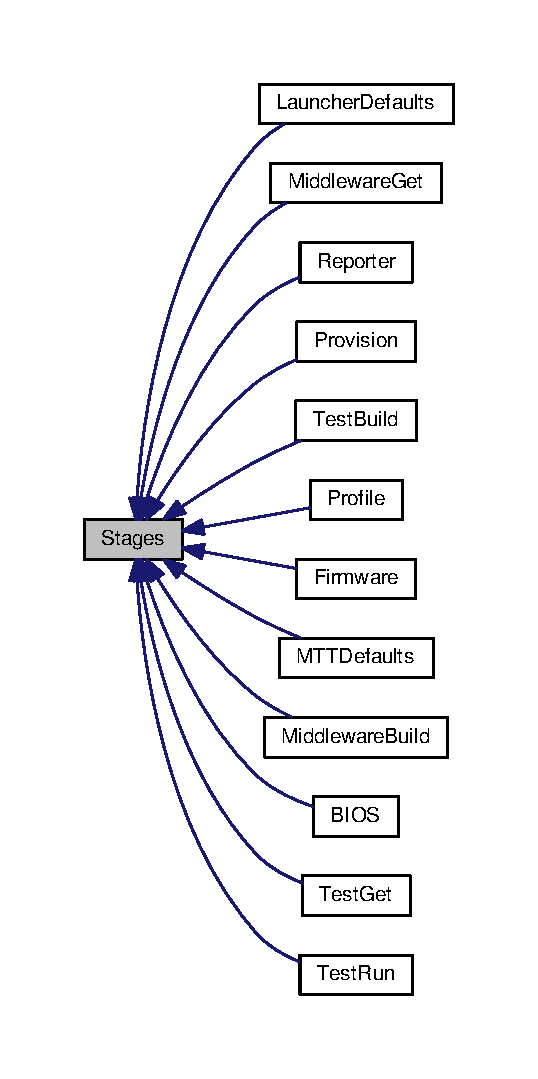
\includegraphics[width=258pt]{group___stages}
\end{center}
\end{figure}
\subsection*{Modules}
\begin{DoxyCompactItemize}
\item 
\hyperlink{group___b_i_o_s}{B\-I\-O\-S}
\begin{DoxyCompactList}\small\item\em \mbox{[}Ordering 50\mbox{]} B\-I\-O\-S flash and query stage \end{DoxyCompactList}\item 
\hyperlink{group___firmware}{Firmware}
\begin{DoxyCompactList}\small\item\em \mbox{[}Ordering 100\mbox{]} Firmware flash and query stage \end{DoxyCompactList}\item 
\hyperlink{group___launcher_defaults}{Launcher\-Defaults}
\begin{DoxyCompactList}\small\item\em \mbox{[}Ordering 490\mbox{]} Allow a user to set default values for a specific launcher \end{DoxyCompactList}\item 
\hyperlink{group___middleware_build}{Middleware\-Build}
\begin{DoxyCompactList}\small\item\em \mbox{[}Ordering 400\mbox{]} Stage for building middleware such as M\-P\-I \end{DoxyCompactList}\item 
\hyperlink{group___middleware_get}{Middleware\-Get}
\begin{DoxyCompactList}\small\item\em \mbox{[}Ordering 300\mbox{]} Stage for getting middleware source code \end{DoxyCompactList}\item 
\hyperlink{group___m_t_t_defaults}{M\-T\-T\-Defaults}
\begin{DoxyCompactList}\small\item\em \mbox{[}Ordering 0\mbox{]} Set M\-T\-T defaults for this test definition \end{DoxyCompactList}\item 
\hyperlink{group___profile}{Profile}
\begin{DoxyCompactList}\small\item\em \mbox{[}Ordering 210\mbox{]} Stage for profiling the system upon which the tests will be conducted \end{DoxyCompactList}\item 
\hyperlink{group___provision}{Provision}
\begin{DoxyCompactList}\small\item\em \mbox{[}Ordering 200\mbox{]} Provisioning stage \end{DoxyCompactList}\item 
\hyperlink{group___reporter}{Reporter}
\begin{DoxyCompactList}\small\item\em \mbox{[}Ordering 600\mbox{]} Report tests results stage \end{DoxyCompactList}\item 
\hyperlink{group___test_build}{Test\-Build}
\begin{DoxyCompactList}\small\item\em \mbox{[}Ordering 475\mbox{]} Build test software package \end{DoxyCompactList}\item 
\hyperlink{group___test_get}{Test\-Get}
\begin{DoxyCompactList}\small\item\em \mbox{[}Ordering 450\mbox{]} Get test software package \end{DoxyCompactList}\item 
\hyperlink{group___test_run}{Test\-Run}
\begin{DoxyCompactList}\small\item\em \mbox{[}Ordering 500\mbox{]} Run test software package \end{DoxyCompactList}\end{DoxyCompactItemize}


\subsection{Detailed Description}
Stages of test execution. 
\hypertarget{group___b_i_o_s}{\section{B\-I\-O\-S}
\label{group___b_i_o_s}\index{B\-I\-O\-S@{B\-I\-O\-S}}
}


\mbox{[}Ordering 50\mbox{]} B\-I\-O\-S flash and query stage  


Collaboration diagram for B\-I\-O\-S\-:
\nopagebreak
\begin{figure}[H]
\begin{center}
\leavevmode
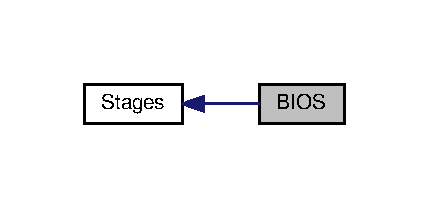
\includegraphics[width=206pt]{group___b_i_o_s}
\end{center}
\end{figure}
\mbox{[}Ordering 50\mbox{]} B\-I\-O\-S flash and query stage 
\hypertarget{group___firmware}{\section{Firmware}
\label{group___firmware}\index{Firmware@{Firmware}}
}


\mbox{[}Ordering 100\mbox{]} Firmware flash and query stage  


Collaboration diagram for Firmware\-:
\nopagebreak
\begin{figure}[H]
\begin{center}
\leavevmode
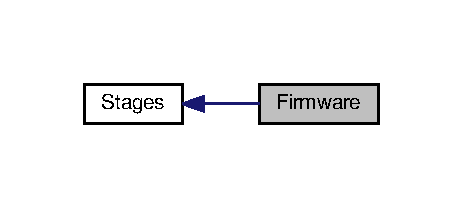
\includegraphics[width=222pt]{group___firmware}
\end{center}
\end{figure}
\mbox{[}Ordering 100\mbox{]} Firmware flash and query stage \hypertarget{FooFlash.py_FooFlash}{}\subsection{Foo\-Flash}\label{FooFlash.py_FooFlash}

\hypertarget{group___launcher_defaults}{\section{Launcher\-Defaults}
\label{group___launcher_defaults}\index{Launcher\-Defaults@{Launcher\-Defaults}}
}


\mbox{[}Ordering 490\mbox{]} Allow a user to set default values for a specific launcher  


Collaboration diagram for Launcher\-Defaults\-:
\nopagebreak
\begin{figure}[H]
\begin{center}
\leavevmode
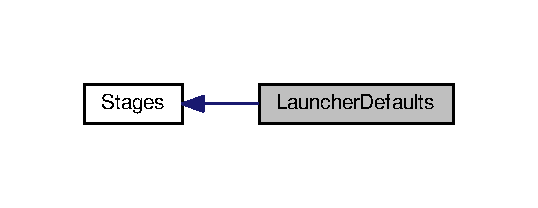
\includegraphics[width=258pt]{group___launcher_defaults}
\end{center}
\end{figure}
\mbox{[}Ordering 490\mbox{]} Allow a user to set default values for a specific launcher 
\hypertarget{group___middleware_build}{\section{Middleware\-Build}
\label{group___middleware_build}\index{Middleware\-Build@{Middleware\-Build}}
}


\mbox{[}Ordering 400\mbox{]} Stage for building middleware such as M\-P\-I  


Collaboration diagram for Middleware\-Build\-:
\nopagebreak
\begin{figure}[H]
\begin{center}
\leavevmode
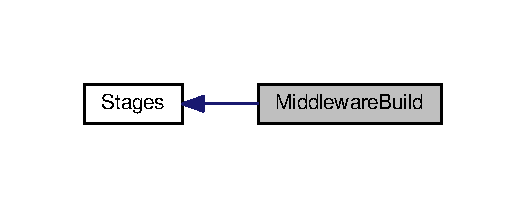
\includegraphics[width=252pt]{group___middleware_build}
\end{center}
\end{figure}
\mbox{[}Ordering 400\mbox{]} Stage for building middleware such as M\-P\-I 
\hypertarget{group___middleware_get}{\section{Middleware\-Get}
\label{group___middleware_get}\index{Middleware\-Get@{Middleware\-Get}}
}


\mbox{[}Ordering 300\mbox{]} Stage for getting middleware source code  


Collaboration diagram for Middleware\-Get\-:
\nopagebreak
\begin{figure}[H]
\begin{center}
\leavevmode
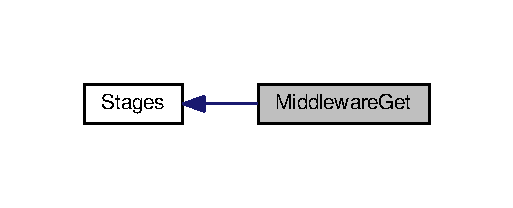
\includegraphics[width=246pt]{group___middleware_get}
\end{center}
\end{figure}
\mbox{[}Ordering 300\mbox{]} Stage for getting middleware source code 
\hypertarget{group___m_t_t_defaults}{\section{M\-T\-T\-Defaults}
\label{group___m_t_t_defaults}\index{M\-T\-T\-Defaults@{M\-T\-T\-Defaults}}
}


\mbox{[}Ordering 0\mbox{]} Set M\-T\-T defaults for this test definition  


Collaboration diagram for M\-T\-T\-Defaults\-:
\nopagebreak
\begin{figure}[H]
\begin{center}
\leavevmode
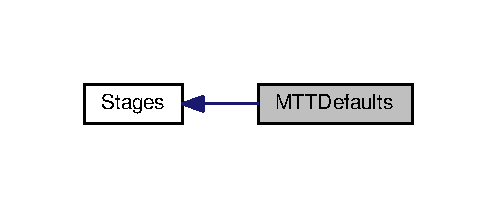
\includegraphics[width=238pt]{group___m_t_t_defaults}
\end{center}
\end{figure}
\mbox{[}Ordering 0\mbox{]} Set M\-T\-T defaults for this test definition \hypertarget{group___m_t_t_defaults_DefaultMTTDefaults}{}\subsection{Default\-M\-T\-T\-Defaults}\label{group___m_t_t_defaults_DefaultMTTDefaults}
Store any provided default M\-T\-T settings 
\begin{DoxyParams}{Parameters}
{\em trial} & Use when testing your M\-T\-T client setup; results that are generated and submitted to the database are marked as "trials" and are not included in normal reporting. \\
\hline
{\em scratchdir} & Specify the D\-I\-R\-E\-C\-T\-O\-R\-Y under which scratch files are to be stored \\
\hline
{\em description} & Provide a brief title/description to be included in the log for this test \\
\hline
{\em platform} & Name of the system under test \\
\hline
{\em organization} & Name of the organization running the test \\
\hline
{\em merge\-\_\-stdout\-\_\-stderr} & Merge stdout and stderr into one output stream \\
\hline
{\em stdout\-\_\-save\-\_\-lines} & Number of lines of stdout to save (-\/1 for unlimited) \\
\hline
{\em stderr\-\_\-save\-\_\-lines} & Number of lines of stderr to save (-\/1 for unlimited) \\
\hline
{\em executor} & Strategy to use\-: combinatorial or sequential executor \\
\hline
{\em time} & Record how long it takes to run each individual test \\
\hline
\end{DoxyParams}

\hypertarget{group___profile}{\section{Profile}
\label{group___profile}\index{Profile@{Profile}}
}


\mbox{[}Ordering 210\mbox{]} Stage for profiling the system upon which the tests will be conducted  


Collaboration diagram for Profile\-:
\nopagebreak
\begin{figure}[H]
\begin{center}
\leavevmode
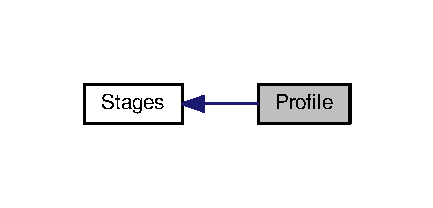
\includegraphics[width=208pt]{group___profile}
\end{center}
\end{figure}
\mbox{[}Ordering 210\mbox{]} Stage for profiling the system upon which the tests will be conducted \hypertarget{group___profile_CheckProfile}{}\subsection{Check\-Profile}\label{group___profile_CheckProfile}
Check hardware and software profile value of the system against a threshold 
\begin{DoxyParams}{Parameters}
{\em disk\-Space} & check a disks \% avail (/opt $>$= 10\%) \\
\hline
{\em memory} & check free, used or total memory value in G (free $>$= 5\-G)\\
\hline
\end{DoxyParams}
\hypertarget{group___profile_DefaultProfile}{}\subsection{Default\-Profile}\label{group___profile_DefaultProfile}
Collect hardware and software profile of the system 
\begin{DoxyParams}{Parameters}
{\em kernel\-Name} & Kernel name \\
\hline
{\em kernel\-Release} & Kernel release string \\
\hline
{\em kernel\-Version} & Kernel version string \\
\hline
{\em machine\-Name} & Machine name \\
\hline
{\em processor\-Type} & Processor type \\
\hline
{\em node\-Name} & Node name \\
\hline
\end{DoxyParams}

\hypertarget{group___provision}{\section{Provision}
\label{group___provision}\index{Provision@{Provision}}
}


\mbox{[}Ordering 200\mbox{]} Provisioning stage  


Collaboration diagram for Provision\-:
\nopagebreak
\begin{figure}[H]
\begin{center}
\leavevmode
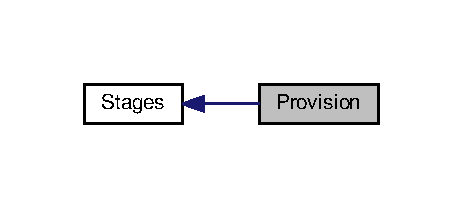
\includegraphics[width=222pt]{group___provision}
\end{center}
\end{figure}
\mbox{[}Ordering 200\mbox{]} Provisioning stage \hypertarget{group___provision_WWulf3}{}\subsection{W\-Wulf3}\label{group___provision_WWulf3}
Plugin for provisioning nodes using the Warewulf v3 image manager 
\begin{DoxyParams}{Parameters}
{\em target} & List of remote host names or L\-A\-N interfaces to be provisioned \\
\hline
{\em image} & Name of image to be instantiated \\
\hline
{\em bootstrap} & Name of bootstrap to be used \\
\hline
{\em controller} & List of I\-P addresses of remote node controllers/\-B\-M\-Cs \\
\hline
{\em username} & Remote controller username \\
\hline
{\em password} & Remote controller password \\
\hline
{\em pwfile} & File containing remote controller password \\
\hline
{\em sudo} & Use sudo to execute privileged commands \\
\hline
{\em allocate\-\_\-cmd} & Command to use for allocating nodes from the resource manager \\
\hline
{\em deallocate\-\_\-cmd} & Command to use for deallocating nodes from the resource manager \\
\hline
\end{DoxyParams}

\hypertarget{group___reporter}{\section{Reporter}
\label{group___reporter}\index{Reporter@{Reporter}}
}


\mbox{[}Ordering 600\mbox{]} Report tests results stage  


Collaboration diagram for Reporter\-:
\nopagebreak
\begin{figure}[H]
\begin{center}
\leavevmode
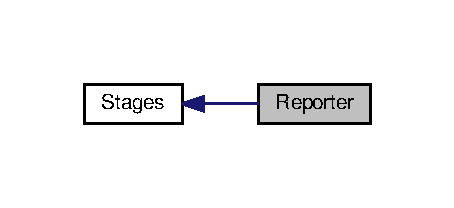
\includegraphics[width=218pt]{group___reporter}
\end{center}
\end{figure}
\mbox{[}Ordering 600\mbox{]} Report tests results stage \hypertarget{group___reporter_IUDatabase}{}\subsection{I\-U\-Database}\label{group___reporter_IUDatabase}
M\-T\-T Database reporter plugin for the legacy I\-U submission server 
\begin{DoxyParams}{Parameters}
{\em realm} & Database name \\
\hline
{\em username} & Username to be used for submitting data \\
\hline
{\em password} & Password for that username \\
\hline
{\em pwfile} & File where password can be found \\
\hline
{\em platform} & Name of the platform (cluster) upon which the tests were run \\
\hline
{\em hostname} & Name of the hosts involved in the tests (may be regular expression) \\
\hline
{\em url} & U\-R\-L of the database server \\
\hline
{\em debug\-\_\-filename} & Debug output file for server interaction information \\
\hline
{\em keep\-\_\-debug\-\_\-files} & Retain reporter debug output after execution \\
\hline
{\em debug\-\_\-server} & Ask the server to return its debug output as well \\
\hline
{\em email} & Email to which errors are to be sent\\
\hline
\end{DoxyParams}
\hypertarget{group___reporter_JunitXML}{}\subsection{Junit\-X\-M\-L}\label{group___reporter_JunitXML}
Junit X\-M\-L plugin 
\begin{DoxyParams}{Parameters}
{\em filename} & Name of the file into which the report is to be written \\
\hline
{\em textwrap} & Max line length before wrapping\\
\hline
\end{DoxyParams}
\hypertarget{group___reporter_TextFile}{}\subsection{Text\-File}\label{group___reporter_TextFile}
File reporter plugin 
\begin{DoxyParams}{Parameters}
{\em filename} & Name of the file into which the report is to be written \\
\hline
{\em summary\-\_\-footer} & Footer to be placed at bottom of summary \\
\hline
{\em detail\-\_\-header} & Header to be put at top of detail report \\
\hline
{\em detail\-\_\-footer} & Footer to be placed at bottome of detail report \\
\hline
{\em textwrap} & Max line length before wrapping \\
\hline
\end{DoxyParams}

\hypertarget{group___test_build}{\section{Test\-Build}
\label{group___test_build}\index{Test\-Build@{Test\-Build}}
}


\mbox{[}Ordering 475\mbox{]} Build test software package  


Collaboration diagram for Test\-Build\-:
\nopagebreak
\begin{figure}[H]
\begin{center}
\leavevmode
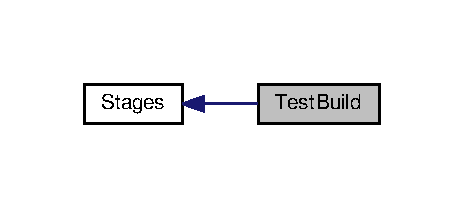
\includegraphics[width=222pt]{group___test_build}
\end{center}
\end{figure}
\mbox{[}Ordering 475\mbox{]} Build test software package 
\hypertarget{group___test_get}{\section{Test\-Get}
\label{group___test_get}\index{Test\-Get@{Test\-Get}}
}


\mbox{[}Ordering 450\mbox{]} Get test software package  


Collaboration diagram for Test\-Get\-:
\nopagebreak
\begin{figure}[H]
\begin{center}
\leavevmode
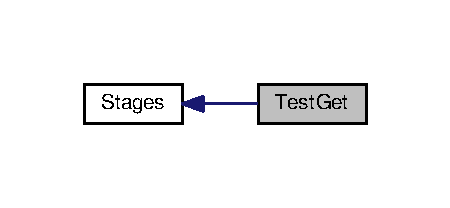
\includegraphics[width=216pt]{group___test_get}
\end{center}
\end{figure}
\mbox{[}Ordering 450\mbox{]} Get test software package 
\hypertarget{group___test_run}{\section{Test\-Run}
\label{group___test_run}\index{Test\-Run@{Test\-Run}}
}


\mbox{[}Ordering 500\mbox{]} Run test software package  


Collaboration diagram for Test\-Run\-:
\nopagebreak
\begin{figure}[H]
\begin{center}
\leavevmode
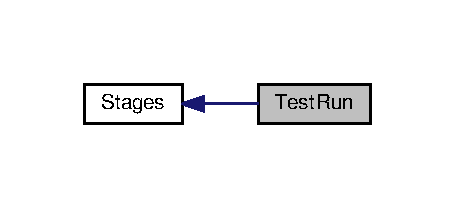
\includegraphics[width=218pt]{group___test_run}
\end{center}
\end{figure}
\mbox{[}Ordering 500\mbox{]} Run test software package 
\hypertarget{group___tools}{\section{Tools}
\label{group___tools}\index{Tools@{Tools}}
}


Plugins required by Stages.  


Collaboration diagram for Tools\-:
\nopagebreak
\begin{figure}[H]
\begin{center}
\leavevmode
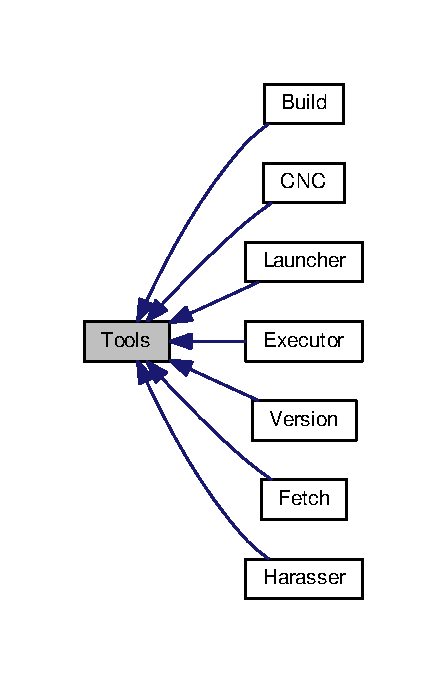
\includegraphics[width=214pt]{group___tools}
\end{center}
\end{figure}
\subsection*{Modules}
\begin{DoxyCompactItemize}
\item 
\hyperlink{group___build}{Build}
\begin{DoxyCompactList}\small\item\em Build tools for test content. \end{DoxyCompactList}\item 
\hyperlink{group___c_n_c}{C\-N\-C}
\begin{DoxyCompactList}\small\item\em Comand and control tools for system managment. \end{DoxyCompactList}\item 
\hyperlink{group___executor}{Executor}
\begin{DoxyCompactList}\small\item\em Executor of test description. \end{DoxyCompactList}\item 
\hyperlink{group___fetch}{Fetch}
\begin{DoxyCompactList}\small\item\em Tools for fetching tests. \end{DoxyCompactList}\item 
\hyperlink{group___harasser}{Harasser}
\begin{DoxyCompactList}\small\item\em \hyperlink{namespace_harasser}{Harasser} tools for test content. \end{DoxyCompactList}\item 
\hyperlink{group___launcher}{Launcher}
\begin{DoxyCompactList}\small\item\em Tools for launching H\-P\-C jobs. \end{DoxyCompactList}\item 
\hyperlink{group___version}{Version}
\begin{DoxyCompactList}\small\item\em Tools that collect version information. \end{DoxyCompactList}\end{DoxyCompactItemize}


\subsection{Detailed Description}
Plugins required by Stages. 
\hypertarget{group___utilities}{\section{Utilities}
\label{group___utilities}\index{Utilities@{Utilities}}
}


Plugins used by the M\-T\-T framework.  


Plugins used by the M\-T\-T framework. \hypertarget{group___utilities_Compilers}{}\subsection{Compilers}\label{group___utilities_Compilers}
Identify the type and version of compilers in-\/use\hypertarget{group___utilities_Copy}{}\subsection{Copy}\label{group___utilities_Copy}
\hyperlink{namespace_copy}{Copy} a comma separated list of files, directories, and links 
\begin{DoxyParams}{Parameters}
{\em src} & The name of the file, directory, or link to be copied \\
\hline
{\em preserve\-\_\-symlinks} & Preserve symlinks found inside directories\\
\hline
\end{DoxyParams}
\hypertarget{group___utilities_Copytree}{}\subsection{Copytree}\label{group___utilities_Copytree}
\hyperlink{namespace_copy}{Copy} a directory tree from source to the same relative loation under the M\-T\-T scratch directory 
\begin{DoxyParams}{Parameters}
{\em src} & The top directory of the tree to be copied \\
\hline
{\em preserve\-\_\-symlinks} & Preserve symlinks instead of copying the contents \\
\hline
{\em preserve\-\_\-directory} & Copies directory instead of contents\\
\hline
\end{DoxyParams}
\hypertarget{group___utilities_Environ}{}\subsection{Environ}\label{group___utilities_Environ}
Set environment variables\hypertarget{group___utilities_ExecuteCmd}{}\subsection{Execute\-Cmd}\label{group___utilities_ExecuteCmd}
Execute a command and capture its stdout and stderr\hypertarget{group___utilities_Logger}{}\subsection{Logger}\label{group___utilities_Logger}
Log results and provide debug output when directed\hypertarget{group___utilities_ModuleCmd}{}\subsection{Module\-Cmd}\label{group___utilities_ModuleCmd}
Load/\-Unload an environmental module\hypertarget{group___utilities_MPIVersion}{}\subsection{M\-P\-I\-Version}\label{group___utilities_MPIVersion}
Identify the name and version of M\-P\-I in-\/use\hypertarget{group___utilities_Watchdog}{}\subsection{Watchdog}\label{group___utilities_Watchdog}
Generate and exception after a given amount of time 
\begin{DoxyParams}{Parameters}
{\em timeout} & Time in seconds before generating exception \\
\hline
\end{DoxyParams}

\hypertarget{group___build}{\section{Build}
\label{group___build}\index{Build@{Build}}
}


Build tools for test content.  


Collaboration diagram for Build\-:
\nopagebreak
\begin{figure}[H]
\begin{center}
\leavevmode
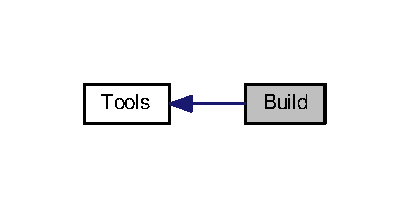
\includegraphics[width=196pt]{group___build}
\end{center}
\end{figure}
Build tools for test content. \hypertarget{group___build_Autotools}{}\subsection{Autotools}\label{group___build_Autotools}
Run typical autotools commands to configure and build a software package 
\begin{DoxyParams}{Parameters}
{\em middleware} & Middleware stage that these tests are to be built against \\
\hline
{\em parent} & Section that precedes this one in the dependency tree \\
\hline
{\em autogen\-\_\-cmd} & Command to be executed to setup the configure script, usually called autogen.\-sh or autogen.\-pl \\
\hline
{\em configure\-\_\-options} & Options to be passed to configure. Note that the prefix will be automatically set and need not be provided here \\
\hline
{\em make\-\_\-options} & Options to be passed to the make command \\
\hline
{\em build\-\_\-in\-\_\-place} & Build tests in current location (no prefix or install) \\
\hline
{\em merge\-\_\-stdout\-\_\-stderr} & Merge stdout and stderr into one output stream \\
\hline
{\em stdout\-\_\-save\-\_\-lines} & Number of lines of stdout to save \\
\hline
{\em stderr\-\_\-save\-\_\-lines} & Number of lines of stderr to save \\
\hline
{\em modules\-\_\-unload} & Modules to unload \\
\hline
{\em modules} & Modules to load \\
\hline
{\em modules\-\_\-swap} & Modules to swap\\
\hline
\end{DoxyParams}
\hypertarget{group___build_Hostfile}{}\subsection{Hostfile}\label{group___build_Hostfile}
Builds a hostfile based on a nodelist 
\begin{DoxyParams}{Parameters}
{\em parent} & Section that precedes this one in the dependency tree \\
\hline
{\em nodelist} & list of nodes to create hostfile from \\
\hline
{\em hostfile} & name of hostfile to generate\\
\hline
\end{DoxyParams}
\hypertarget{group___build_Shell}{}\subsection{Shell}\label{group___build_Shell}
Run shell commands to configure and build a software package 
\begin{DoxyParams}{Parameters}
{\em middleware} & Middleware stage that these tests are to be built against \\
\hline
{\em command} & Command to execute \\
\hline
{\em parent} & Section that precedes this one in the dependency tree \\
\hline
{\em merge\-\_\-stdout\-\_\-stderr} & Merge stdout and stderr into one output stream \\
\hline
{\em stdout\-\_\-save\-\_\-lines} & Number of lines of stdout to save \\
\hline
{\em stderr\-\_\-save\-\_\-lines} & Number of lines of stderr to save \\
\hline
{\em modules\-\_\-unload} & Modules to unload \\
\hline
{\em modules} & Modules to load \\
\hline
{\em modules\-\_\-swap} & Modules to swap \\
\hline
{\em fail\-\_\-test} & Specifies whether this test is expected to fail (value=None means test is expected to succeed) \\
\hline
{\em fail\-\_\-returncode} & Specifies the expected failure returncode of this test \\
\hline
{\em allocate\-\_\-cmd} & Command to use for allocating nodes from the resource manager \\
\hline
{\em deallocate\-\_\-cmd} & Command to use for deallocating nodes from the resource manager \\
\hline
{\em asis\-\_\-target} & Specifies name of asis\-\_\-target being built. This is used with "A\-S\-I\-S" keyword to determine whether to do anything. \\
\hline
\end{DoxyParams}

\hypertarget{group___c_n_c}{\section{C\-N\-C}
\label{group___c_n_c}\index{C\-N\-C@{C\-N\-C}}
}


Comand and control tools for system managment.  


Collaboration diagram for C\-N\-C\-:
\nopagebreak
\begin{figure}[H]
\begin{center}
\leavevmode
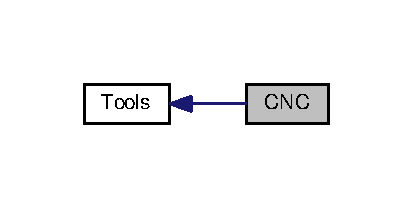
\includegraphics[width=198pt]{group___c_n_c}
\end{center}
\end{figure}
Comand and control tools for system managment. \hypertarget{group___c_n_c_IPMITool}{}\subsection{I\-P\-M\-I\-Tool}\label{group___c_n_c_IPMITool}
Interface to the ipmitool cmd line 
\begin{DoxyParams}{Parameters}
{\em target} & List of remote host names or L\-A\-N interfaces to monitor during reset operations \\
\hline
{\em controller} & List of I\-P addresses of remote node controllers/\-B\-M\-Cs \\
\hline
{\em username} & Remote session username \\
\hline
{\em password} & Remote session password \\
\hline
{\em pwfile} & File containing remote session password \\
\hline
{\em command} & Command to be sent \\
\hline
{\em maxtries} & Max number of times to ping each host before declaring reset to fail \\
\hline
{\em numthreads} & Number of worker threads to use \\
\hline
{\em dryrun} & Dryrun -\/ print out commands but do not execute \\
\hline
{\em sudo} & Use sudo to exeute privilaged comands \\
\hline
\end{DoxyParams}

\hypertarget{group___executor}{\section{Executor}
\label{group___executor}\index{Executor@{Executor}}
}


Executor of test description.  


Collaboration diagram for Executor\-:
\nopagebreak
\begin{figure}[H]
\begin{center}
\leavevmode
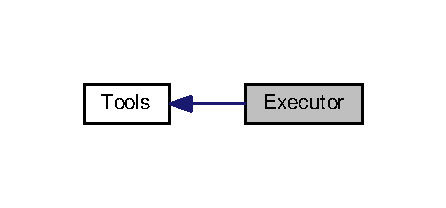
\includegraphics[width=214pt]{group___executor}
\end{center}
\end{figure}
Executor of test description. \hypertarget{group___executor_CombinatorialEx}{}\subsection{Combinatorial\-Ex}\label{group___executor_CombinatorialEx}
Combinatorial execution executor\hypertarget{group___executor_SequentialEx}{}\subsection{Sequential\-Ex}\label{group___executor_SequentialEx}
Sequential execution executor 
\hypertarget{group___fetch}{\section{Fetch}
\label{group___fetch}\index{Fetch@{Fetch}}
}


Tools for fetching tests.  


Collaboration diagram for Fetch\-:
\nopagebreak
\begin{figure}[H]
\begin{center}
\leavevmode
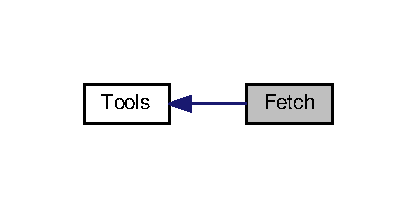
\includegraphics[width=200pt]{group___fetch}
\end{center}
\end{figure}
Tools for fetching tests. \hypertarget{group___fetch_AlreadyInstalled}{}\subsection{Already\-Installed}\label{group___fetch_AlreadyInstalled}
No-\/op plugin for using existing middleware installation 
\begin{DoxyParams}{Parameters}
{\em exec} & Executable that should be in path \\
\hline
{\em modules\-\_\-unload} & Modules to unload \\
\hline
{\em modules} & Modules to load \\
\hline
{\em modules\-\_\-swap} & Modules to swap\\
\hline
\end{DoxyParams}
\hypertarget{group___fetch_Git}{}\subsection{Git}\label{group___fetch_Git}
Plugin for getting software via \hyperlink{namespace_git}{Git} 
\begin{DoxyParams}{Parameters}
{\em url} & U\-R\-L to access the repository \\
\hline
{\em username} & Username required for accessing the repository \\
\hline
{\em password} & Password required for that user to access the repository \\
\hline
{\em pwfile} & File where password can be found \\
\hline
{\em branch} & Branch (if not master) to be downloaded \\
\hline
{\em pr} & Pull request to be downloaded \\
\hline
{\em subdir} & Subdirectory of interest in repository \\
\hline
{\em modules\-\_\-unload} & Modules to unload \\
\hline
{\em modules} & Modules to load \\
\hline
{\em modules\-\_\-swap} & Modules to swap\\
\hline
\end{DoxyParams}
\hypertarget{group___fetch_OMPI_Snapshot}{}\subsection{O\-M\-P\-I\-\_\-\-Snapshot}\label{group___fetch_OMPI_Snapshot}
Plugin for getting software via O\-M\-P\-I Nightly tarballs 
\begin{DoxyParams}{Parameters}
{\em url} & U\-R\-L to access the O\-M\-P\-I nightly tarball (e.\-g. \href{https://www.open-mpi.org/nightly/v2.x}{\tt https\-://www.\-open-\/mpi.\-org/nightly/v2.\-x}) \\
\hline
{\em version\-\_\-file} & optional file containing name of most recent tarball version tested \\
\hline
{\em mpi\-\_\-name} & optional name for the O\-M\-P\-I snapshot tarball \\
\hline
\end{DoxyParams}

\hypertarget{group___harasser}{\section{Harasser}
\label{group___harasser}\index{Harasser@{Harasser}}
}


\hyperlink{namespace_harasser}{Harasser} tools for test content.  


Collaboration diagram for Harasser\-:
\nopagebreak
\begin{figure}[H]
\begin{center}
\leavevmode
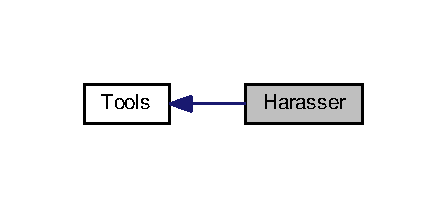
\includegraphics[width=214pt]{group___harasser}
\end{center}
\end{figure}
\hyperlink{namespace_harasser}{Harasser} tools for test content. \hypertarget{group___harasser_Harasser}{}\subsection{Harasser}\label{group___harasser_Harasser}
Run harasser scripts while test-\/content is running 
\begin{DoxyParams}{Parameters}
{\em trigger\-\_\-scripts} & Scripts to run to launch harassers \\
\hline
{\em stop\-\_\-scripts} & Scripts to run to stop and clean-\/up harassers \\
\hline
{\em join\-\_\-timeout} & Seconds to wait for process to finish \\
\hline
\end{DoxyParams}

\hypertarget{group___launcher}{\section{Launcher}
\label{group___launcher}\index{Launcher@{Launcher}}
}


Tools for launching H\-P\-C jobs.  


Collaboration diagram for Launcher\-:
\nopagebreak
\begin{figure}[H]
\begin{center}
\leavevmode
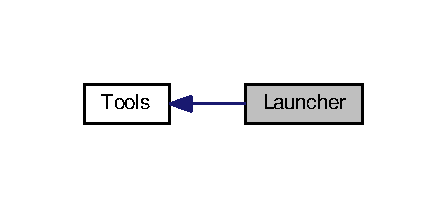
\includegraphics[width=214pt]{group___launcher}
\end{center}
\end{figure}
Tools for launching H\-P\-C jobs. \hypertarget{group___launcher_ALPS}{}\subsection{A\-L\-P\-S}\label{group___launcher_ALPS}
Plugin for using \hyperlink{namespace_a_l_p_s}{A\-L\-P\-S} to launch tests 
\begin{DoxyParams}{Parameters}
{\em hostfile} & The hostfile for \hyperlink{namespace_open_m_p_i}{Open\-M\-P\-I} to use \\
\hline
{\em command} & Command for executing the application \\
\hline
{\em np} & Number of processes to run \\
\hline
{\em options} & Comma-\/delimited sets of command line options that shall be used on each test \\
\hline
{\em skipped} & Exit status of a test that declares it was skipped \\
\hline
{\em merge\-\_\-stdout\-\_\-stderr} & Merge stdout and stderr into one output stream \\
\hline
{\em stdout\-\_\-save\-\_\-lines} & Number of lines of stdout to save \\
\hline
{\em stderr\-\_\-save\-\_\-lines} & Number of lines of stderr to save \\
\hline
{\em test\-\_\-dir} & Names of directories to be scanned for tests \\
\hline
{\em fail\-\_\-tests} & Names of tests that are expected to fail \\
\hline
{\em fail\-\_\-returncodes} & Expected returncodes of tests expected to fail \\
\hline
{\em fail\-\_\-timeout} & Maximum execution time for tests expected to fail \\
\hline
{\em skip\-\_\-tests} & Names of tests to be skipped \\
\hline
{\em max\-\_\-num\-\_\-tests} & Maximum number of tests to run \\
\hline
{\em modules} & Modules to load \\
\hline
{\em modules\-\_\-unload} & Modules to unload \\
\hline
{\em test\-\_\-list} & List of tests to run, default is all \\
\hline
{\em allocate\-\_\-cmd} & Command to use for allocating nodes from the resource manager \\
\hline
{\em deallocate\-\_\-cmd} & Command to use for deallocating nodes from the resource manager\\
\hline
\end{DoxyParams}
\hypertarget{group___launcher_OpenMPI}{}\subsection{Open\-M\-P\-I}\label{group___launcher_OpenMPI}
Plugin for using the Open M\-P\-I mpirun launch tool 
\begin{DoxyParams}{Parameters}
{\em hostfile} & The hostfile for \hyperlink{namespace_open_m_p_i}{Open\-M\-P\-I} to use \\
\hline
{\em command} & Command for executing the application \\
\hline
{\em np} & Number of processes to run \\
\hline
{\em ppn} & Number of processes per node to run \\
\hline
{\em timeout} & Maximum execution time -\/ terminate a test if it exceeds this time \\
\hline
{\em options} & Comma-\/delimited sets of command line options that shall be used on each test \\
\hline
{\em skipped} & Exit status of a test that declares it was skipped \\
\hline
{\em merge\-\_\-stdout\-\_\-stderr} & Merge stdout and stderr into one output stream \\
\hline
{\em stdout\-\_\-save\-\_\-lines} & Number of lines of stdout to save \\
\hline
{\em stderr\-\_\-save\-\_\-lines} & Number of lines of stderr to save \\
\hline
{\em test\-\_\-dir} & Names of directories to be scanned for tests \\
\hline
{\em fail\-\_\-tests} & Names of tests that are expected to fail \\
\hline
{\em fail\-\_\-returncodes} & Expected return codes of tests expected to fail \\
\hline
{\em fail\-\_\-timeout} & Maximum execution time for tests expected to fail \\
\hline
{\em skip\-\_\-tests} & Names of tests to be skipped \\
\hline
{\em max\-\_\-num\-\_\-tests} & Maximum number of tests to run \\
\hline
{\em test\-\_\-list} & List of tests to run, default is all \\
\hline
{\em allocate\-\_\-cmd} & Command to use for allocating nodes from the resource manager \\
\hline
{\em deallocate\-\_\-cmd} & Command to use for deallocating nodes from the resource manager\\
\hline
\end{DoxyParams}
\hypertarget{group___launcher_SLURM}{}\subsection{S\-L\-U\-R\-M}\label{group___launcher_SLURM}
Plugin for using \hyperlink{namespace_s_l_u_r_m}{S\-L\-U\-R\-M} to launch tests 
\begin{DoxyParams}{Parameters}
{\em hostfile} & The hostfile for \hyperlink{namespace_open_m_p_i}{Open\-M\-P\-I} to use \\
\hline
{\em command} & Command for executing the application \\
\hline
{\em np} & Number of processes to run \\
\hline
{\em timeout} & Maximum execution time -\/ terminate a test if it exceeds this time \\
\hline
{\em options} & Comma-\/delimited sets of command line options that shall be used on each test \\
\hline
{\em skipped} & Exit status of a test that declares it was skipped \\
\hline
{\em merge\-\_\-stdout\-\_\-stderr} & Merge stdout and stderr into one output stream \\
\hline
{\em stdout\-\_\-save\-\_\-lines} & Number of lines of stdout to save \\
\hline
{\em stderr\-\_\-save\-\_\-lines} & Number of lines of stderr to save \\
\hline
{\em test\-\_\-dir} & Names of directories to be scanned for tests \\
\hline
{\em fail\-\_\-tests} & Names of tests that are expected to fail \\
\hline
{\em fail\-\_\-returncodes} & Expected returncodes of tests expected to fail \\
\hline
{\em fail\-\_\-timeout} & Maximum execution time for tests expected to fail \\
\hline
{\em skip\-\_\-tests} & Names of tests to be skipped \\
\hline
{\em max\-\_\-num\-\_\-tests} & Maximum number of tests to run \\
\hline
{\em job\-\_\-name} & User-\/defined name for job \\
\hline
{\em modules} & Modules to load \\
\hline
{\em modules\-\_\-unload} & Modules to unload \\
\hline
{\em test\-\_\-list} & List of tests to run, default is all \\
\hline
{\em allocate\-\_\-cmd} & Command to use for allocating nodes from the resource manager \\
\hline
{\em deallocate\-\_\-cmd} & Command to use for deallocating nodes from the resource manager \\
\hline
\end{DoxyParams}

\hypertarget{group___version}{\section{Version}
\label{group___version}\index{Version@{Version}}
}


Tools that collect version information.  


Collaboration diagram for Version\-:
\nopagebreak
\begin{figure}[H]
\begin{center}
\leavevmode
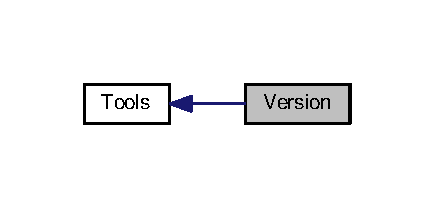
\includegraphics[width=208pt]{group___version}
\end{center}
\end{figure}
Tools that collect version information. \hypertarget{group___version_MTTVersionPlugin}{}\subsection{M\-T\-T\-Version\-Plugin}\label{group___version_MTTVersionPlugin}
A simple plugin for returning the M\-T\-T Version 
\chapter{Namespace Documentation}
\hypertarget{namespace_a_l_p_s}{\section{A\-L\-P\-S Namespace Reference}
\label{namespace_a_l_p_s}\index{A\-L\-P\-S@{A\-L\-P\-S}}
}
\subsection*{Classes}
\begin{DoxyCompactItemize}
\item 
class \hyperlink{class_a_l_p_s_1_1_a_l_p_s}{A\-L\-P\-S}
\end{DoxyCompactItemize}

\hypertarget{namespace_already_installed}{\section{Already\-Installed Namespace Reference}
\label{namespace_already_installed}\index{Already\-Installed@{Already\-Installed}}
}
\subsection*{Classes}
\begin{DoxyCompactItemize}
\item 
class \hyperlink{class_already_installed_1_1_already_installed}{Already\-Installed}
\end{DoxyCompactItemize}

\hypertarget{namespace_autotools}{\section{Autotools Namespace Reference}
\label{namespace_autotools}\index{Autotools@{Autotools}}
}
\subsection*{Classes}
\begin{DoxyCompactItemize}
\item 
class \hyperlink{class_autotools_1_1_autotools}{Autotools}
\end{DoxyCompactItemize}

\hypertarget{namespace_base_m_t_t_utility}{\section{Base\-M\-T\-T\-Utility Namespace Reference}
\label{namespace_base_m_t_t_utility}\index{Base\-M\-T\-T\-Utility@{Base\-M\-T\-T\-Utility}}
}
\subsection*{Classes}
\begin{DoxyCompactItemize}
\item 
class \hyperlink{class_base_m_t_t_utility_1_1_base_m_t_t_utility}{Base\-M\-T\-T\-Utility}
\end{DoxyCompactItemize}

\hypertarget{namespace_b_i_o_s_m_t_t_stage}{\section{B\-I\-O\-S\-M\-T\-T\-Stage Namespace Reference}
\label{namespace_b_i_o_s_m_t_t_stage}\index{B\-I\-O\-S\-M\-T\-T\-Stage@{B\-I\-O\-S\-M\-T\-T\-Stage}}
}
\subsection*{Classes}
\begin{DoxyCompactItemize}
\item 
class \hyperlink{class_b_i_o_s_m_t_t_stage_1_1_b_i_o_s_m_t_t_stage}{B\-I\-O\-S\-M\-T\-T\-Stage}
\end{DoxyCompactItemize}

\hypertarget{namespace_build_m_t_t_tool}{\section{Build\-M\-T\-T\-Tool Namespace Reference}
\label{namespace_build_m_t_t_tool}\index{Build\-M\-T\-T\-Tool@{Build\-M\-T\-T\-Tool}}
}
\subsection*{Classes}
\begin{DoxyCompactItemize}
\item 
class \hyperlink{class_build_m_t_t_tool_1_1_build_m_t_t_tool}{Build\-M\-T\-T\-Tool}
\end{DoxyCompactItemize}

\hypertarget{namespace_check_profile}{\section{Check\-Profile Namespace Reference}
\label{namespace_check_profile}\index{Check\-Profile@{Check\-Profile}}
}
\subsection*{Classes}
\begin{DoxyCompactItemize}
\item 
class \hyperlink{class_check_profile_1_1_check_profile}{Check\-Profile}
\end{DoxyCompactItemize}

\hypertarget{namespace_c_n_c_m_t_t_tool}{\section{C\-N\-C\-M\-T\-T\-Tool Namespace Reference}
\label{namespace_c_n_c_m_t_t_tool}\index{C\-N\-C\-M\-T\-T\-Tool@{C\-N\-C\-M\-T\-T\-Tool}}
}
\subsection*{Classes}
\begin{DoxyCompactItemize}
\item 
class \hyperlink{class_c_n_c_m_t_t_tool_1_1_c_n_c_m_t_t_tool}{C\-N\-C\-M\-T\-T\-Tool}
\end{DoxyCompactItemize}

\hypertarget{namespacecombinatorial}{\section{combinatorial Namespace Reference}
\label{namespacecombinatorial}\index{combinatorial@{combinatorial}}
}
\subsection*{Classes}
\begin{DoxyCompactItemize}
\item 
class \hyperlink{classcombinatorial_1_1_combinatorial_ex}{Combinatorial\-Ex}
\end{DoxyCompactItemize}

\hypertarget{namespace_compilers}{\section{Compilers Namespace Reference}
\label{namespace_compilers}\index{Compilers@{Compilers}}
}
\subsection*{Classes}
\begin{DoxyCompactItemize}
\item 
class \hyperlink{class_compilers_1_1_compilers}{Compilers}
\end{DoxyCompactItemize}

\hypertarget{namespace_copy}{\section{Copy Namespace Reference}
\label{namespace_copy}\index{Copy@{Copy}}
}
\subsection*{Classes}
\begin{DoxyCompactItemize}
\item 
class \hyperlink{class_copy_1_1_copy}{Copy}
\end{DoxyCompactItemize}

\hypertarget{namespace_copytree}{\section{Copytree Namespace Reference}
\label{namespace_copytree}\index{Copytree@{Copytree}}
}
\subsection*{Classes}
\begin{DoxyCompactItemize}
\item 
class \hyperlink{class_copytree_1_1_copytree}{Copytree}
\end{DoxyCompactItemize}

\hypertarget{namespace_default_m_t_t_defaults}{\section{Default\-M\-T\-T\-Defaults Namespace Reference}
\label{namespace_default_m_t_t_defaults}\index{Default\-M\-T\-T\-Defaults@{Default\-M\-T\-T\-Defaults}}
}
\subsection*{Classes}
\begin{DoxyCompactItemize}
\item 
class \hyperlink{class_default_m_t_t_defaults_1_1_default_m_t_t_defaults}{Default\-M\-T\-T\-Defaults}
\end{DoxyCompactItemize}

\hypertarget{namespace_default_profile}{\section{Default\-Profile Namespace Reference}
\label{namespace_default_profile}\index{Default\-Profile@{Default\-Profile}}
}
\subsection*{Classes}
\begin{DoxyCompactItemize}
\item 
class \hyperlink{class_default_profile_1_1_default_profile}{Default\-Profile}
\end{DoxyCompactItemize}

\hypertarget{namespace_default_test_build}{\section{Default\-Test\-Build Namespace Reference}
\label{namespace_default_test_build}\index{Default\-Test\-Build@{Default\-Test\-Build}}
}
\subsection*{Classes}
\begin{DoxyCompactItemize}
\item 
class \hyperlink{class_default_test_build_1_1_default_test_build}{Default\-Test\-Build}
\end{DoxyCompactItemize}

\hypertarget{namespace_environ}{\section{Environ Namespace Reference}
\label{namespace_environ}\index{Environ@{Environ}}
}
\subsection*{Classes}
\begin{DoxyCompactItemize}
\item 
class \hyperlink{class_environ_1_1_environ}{Environ}
\end{DoxyCompactItemize}

\hypertarget{namespace_execute_cmd}{\section{Execute\-Cmd Namespace Reference}
\label{namespace_execute_cmd}\index{Execute\-Cmd@{Execute\-Cmd}}
}
\subsection*{Classes}
\begin{DoxyCompactItemize}
\item 
class \hyperlink{class_execute_cmd_1_1_execute_cmd}{Execute\-Cmd}
\end{DoxyCompactItemize}

\hypertarget{namespace_executor_m_t_t_tool}{\section{Executor\-M\-T\-T\-Tool Namespace Reference}
\label{namespace_executor_m_t_t_tool}\index{Executor\-M\-T\-T\-Tool@{Executor\-M\-T\-T\-Tool}}
}
\subsection*{Classes}
\begin{DoxyCompactItemize}
\item 
class \hyperlink{class_executor_m_t_t_tool_1_1_executor_m_t_t_tool}{Executor\-M\-T\-T\-Tool}
\end{DoxyCompactItemize}

\hypertarget{namespace_fetch_m_t_t_tool}{\section{Fetch\-M\-T\-T\-Tool Namespace Reference}
\label{namespace_fetch_m_t_t_tool}\index{Fetch\-M\-T\-T\-Tool@{Fetch\-M\-T\-T\-Tool}}
}
\subsection*{Classes}
\begin{DoxyCompactItemize}
\item 
class \hyperlink{class_fetch_m_t_t_tool_1_1_fetch_m_t_t_tool}{Fetch\-M\-T\-T\-Tool}
\end{DoxyCompactItemize}

\hypertarget{namespace_firmware_m_t_t_stage}{\section{Firmware\-M\-T\-T\-Stage Namespace Reference}
\label{namespace_firmware_m_t_t_stage}\index{Firmware\-M\-T\-T\-Stage@{Firmware\-M\-T\-T\-Stage}}
}
\subsection*{Classes}
\begin{DoxyCompactItemize}
\item 
class \hyperlink{class_firmware_m_t_t_stage_1_1_firmware_m_t_t_stage}{Firmware\-M\-T\-T\-Stage}
\end{DoxyCompactItemize}

\hypertarget{namespace_foo_flash}{\section{Foo\-Flash Namespace Reference}
\label{namespace_foo_flash}\index{Foo\-Flash@{Foo\-Flash}}
}
\subsection*{Classes}
\begin{DoxyCompactItemize}
\item 
class \hyperlink{class_foo_flash_1_1_foo_flash}{Foo\-Flash}
\end{DoxyCompactItemize}

\hypertarget{namespace_git}{\section{Git Namespace Reference}
\label{namespace_git}\index{Git@{Git}}
}
\subsection*{Classes}
\begin{DoxyCompactItemize}
\item 
class \hyperlink{class_git_1_1_git}{Git}
\end{DoxyCompactItemize}

\hypertarget{namespace_harasser}{\section{Harasser Namespace Reference}
\label{namespace_harasser}\index{Harasser@{Harasser}}
}
\subsection*{Classes}
\begin{DoxyCompactItemize}
\item 
class \hyperlink{class_harasser_1_1_harasser}{Harasser}
\end{DoxyCompactItemize}

\hypertarget{namespace_harasser_m_t_t_tool}{\section{Harasser\-M\-T\-T\-Tool Namespace Reference}
\label{namespace_harasser_m_t_t_tool}\index{Harasser\-M\-T\-T\-Tool@{Harasser\-M\-T\-T\-Tool}}
}
\subsection*{Classes}
\begin{DoxyCompactItemize}
\item 
class \hyperlink{class_harasser_m_t_t_tool_1_1_harasser_m_t_t_tool}{Harasser\-M\-T\-T\-Tool}
\end{DoxyCompactItemize}

\hypertarget{namespace_hostfile}{\section{Hostfile Namespace Reference}
\label{namespace_hostfile}\index{Hostfile@{Hostfile}}
}
\subsection*{Classes}
\begin{DoxyCompactItemize}
\item 
class \hyperlink{class_hostfile_1_1_hostfile}{Hostfile}
\end{DoxyCompactItemize}

\hypertarget{namespace_i_p_m_i_tool}{\section{I\-P\-M\-I\-Tool Namespace Reference}
\label{namespace_i_p_m_i_tool}\index{I\-P\-M\-I\-Tool@{I\-P\-M\-I\-Tool}}
}
\subsection*{Classes}
\begin{DoxyCompactItemize}
\item 
class \hyperlink{class_i_p_m_i_tool_1_1worker_thread}{worker\-Thread}
\item 
class \hyperlink{class_i_p_m_i_tool_1_1_i_p_m_i_tool}{I\-P\-M\-I\-Tool}
\end{DoxyCompactItemize}

\hypertarget{namespace_i_u_database}{\section{I\-U\-Database Namespace Reference}
\label{namespace_i_u_database}\index{I\-U\-Database@{I\-U\-Database}}
}
\subsection*{Classes}
\begin{DoxyCompactItemize}
\item 
class \hyperlink{class_i_u_database_1_1_i_u_database}{I\-U\-Database}
\end{DoxyCompactItemize}

\hypertarget{namespace_junit_x_m_l}{\section{Junit\-X\-M\-L Namespace Reference}
\label{namespace_junit_x_m_l}\index{Junit\-X\-M\-L@{Junit\-X\-M\-L}}
}
\subsection*{Classes}
\begin{DoxyCompactItemize}
\item 
class \hyperlink{class_junit_x_m_l_1_1_junit_x_m_l}{Junit\-X\-M\-L}
\end{DoxyCompactItemize}

\hypertarget{namespace_launcher_defaults_m_t_t_stage}{\section{Launcher\-Defaults\-M\-T\-T\-Stage Namespace Reference}
\label{namespace_launcher_defaults_m_t_t_stage}\index{Launcher\-Defaults\-M\-T\-T\-Stage@{Launcher\-Defaults\-M\-T\-T\-Stage}}
}
\subsection*{Classes}
\begin{DoxyCompactItemize}
\item 
class \hyperlink{class_launcher_defaults_m_t_t_stage_1_1_launcher_defaults_m_t_t_stage}{Launcher\-Defaults\-M\-T\-T\-Stage}
\end{DoxyCompactItemize}

\hypertarget{namespace_launcher_m_t_t_tool}{\section{Launcher\-M\-T\-T\-Tool Namespace Reference}
\label{namespace_launcher_m_t_t_tool}\index{Launcher\-M\-T\-T\-Tool@{Launcher\-M\-T\-T\-Tool}}
}
\subsection*{Classes}
\begin{DoxyCompactItemize}
\item 
class \hyperlink{class_launcher_m_t_t_tool_1_1_launcher_m_t_t_tool}{Launcher\-M\-T\-T\-Tool}
\end{DoxyCompactItemize}

\hypertarget{namespace_load_classes}{\section{Load\-Classes Namespace Reference}
\label{namespace_load_classes}\index{Load\-Classes@{Load\-Classes}}
}
\subsection*{Classes}
\begin{DoxyCompactItemize}
\item 
class \hyperlink{class_load_classes_1_1_load_classes}{Load\-Classes}
\end{DoxyCompactItemize}

\hypertarget{namespace_logger}{\section{Logger Namespace Reference}
\label{namespace_logger}\index{Logger@{Logger}}
}
\subsection*{Classes}
\begin{DoxyCompactItemize}
\item 
class \hyperlink{class_logger_1_1_logger}{Logger}
\end{DoxyCompactItemize}

\hypertarget{namespace_middleware_build_m_t_t_stage}{\section{Middleware\-Build\-M\-T\-T\-Stage Namespace Reference}
\label{namespace_middleware_build_m_t_t_stage}\index{Middleware\-Build\-M\-T\-T\-Stage@{Middleware\-Build\-M\-T\-T\-Stage}}
}
\subsection*{Classes}
\begin{DoxyCompactItemize}
\item 
class \hyperlink{class_middleware_build_m_t_t_stage_1_1_middleware_build_m_t_t_stage}{Middleware\-Build\-M\-T\-T\-Stage}
\end{DoxyCompactItemize}

\hypertarget{namespace_middleware_get_m_t_t_stage}{\section{Middleware\-Get\-M\-T\-T\-Stage Namespace Reference}
\label{namespace_middleware_get_m_t_t_stage}\index{Middleware\-Get\-M\-T\-T\-Stage@{Middleware\-Get\-M\-T\-T\-Stage}}
}
\subsection*{Classes}
\begin{DoxyCompactItemize}
\item 
class \hyperlink{class_middleware_get_m_t_t_stage_1_1_middleware_get_m_t_t_stage}{Middleware\-Get\-M\-T\-T\-Stage}
\end{DoxyCompactItemize}

\hypertarget{namespace_module_cmd}{\section{Module\-Cmd Namespace Reference}
\label{namespace_module_cmd}\index{Module\-Cmd@{Module\-Cmd}}
}
\subsection*{Classes}
\begin{DoxyCompactItemize}
\item 
class \hyperlink{class_module_cmd_1_1_module_cmd}{Module\-Cmd}
\end{DoxyCompactItemize}

\hypertarget{namespace_m_p_i_version}{\section{M\-P\-I\-Version Namespace Reference}
\label{namespace_m_p_i_version}\index{M\-P\-I\-Version@{M\-P\-I\-Version}}
}
\subsection*{Classes}
\begin{DoxyCompactItemize}
\item 
class \hyperlink{class_m_p_i_version_1_1_m_p_i_version}{M\-P\-I\-Version}
\end{DoxyCompactItemize}

\hypertarget{namespace_m_t_t_defaults_m_t_t_stage}{\section{M\-T\-T\-Defaults\-M\-T\-T\-Stage Namespace Reference}
\label{namespace_m_t_t_defaults_m_t_t_stage}\index{M\-T\-T\-Defaults\-M\-T\-T\-Stage@{M\-T\-T\-Defaults\-M\-T\-T\-Stage}}
}
\subsection*{Classes}
\begin{DoxyCompactItemize}
\item 
class \hyperlink{class_m_t_t_defaults_m_t_t_stage_1_1_m_t_t_defaults_m_t_t_stage}{M\-T\-T\-Defaults\-M\-T\-T\-Stage}
\end{DoxyCompactItemize}

\hypertarget{namespace_m_t_t_version_plugin}{\section{M\-T\-T\-Version\-Plugin Namespace Reference}
\label{namespace_m_t_t_version_plugin}\index{M\-T\-T\-Version\-Plugin@{M\-T\-T\-Version\-Plugin}}
}
\subsection*{Classes}
\begin{DoxyCompactItemize}
\item 
class \hyperlink{class_m_t_t_version_plugin_1_1_m_t_t_version_plugin}{M\-T\-T\-Version\-Plugin}
\end{DoxyCompactItemize}
\subsection*{Variables}
\begin{DoxyCompactItemize}
\item 
string \hyperlink{namespace_m_t_t_version_plugin_af9e75ea5f854bed820d4cb64fa455124}{M\-T\-T\-Major} = \char`\"{}4\char`\"{}
\item 
string \hyperlink{namespace_m_t_t_version_plugin_ad80f82936d1bc7547278d4ce2ea3a275}{M\-T\-T\-Minor} = \char`\"{}0\char`\"{}
\item 
string \hyperlink{namespace_m_t_t_version_plugin_a9d8e0707641b9a16174563aacdc82407}{M\-T\-T\-Release} = \char`\"{}0\char`\"{}
\item 
string \hyperlink{namespace_m_t_t_version_plugin_ac27a9d2aec2e835e6f4dc27c68382f38}{M\-T\-T\-Greek} = \char`\"{}a1\char`\"{}
\item 
string \hyperlink{namespace_m_t_t_version_plugin_a51adbd87756e59f2189831112aad767e}{M\-T\-T\-Py\-Client\-Major} = \char`\"{}1\char`\"{}
\item 
string \hyperlink{namespace_m_t_t_version_plugin_aa431ead037b1e7329d119bc1e4017ced}{M\-T\-T\-Py\-Client\-Minor} = \char`\"{}0\char`\"{}
\item 
string \hyperlink{namespace_m_t_t_version_plugin_ae6cedc84f8ae714487299ccdc4403a10}{M\-T\-T\-Py\-Client\-Release} = \char`\"{}0\char`\"{}
\item 
string \hyperlink{namespace_m_t_t_version_plugin_a6df21a21318661784dcabdb81450ff48}{M\-T\-T\-Py\-Client\-Greek} = \char`\"{}a1\char`\"{}
\end{DoxyCompactItemize}


\subsection{Variable Documentation}
\hypertarget{namespace_m_t_t_version_plugin_ac27a9d2aec2e835e6f4dc27c68382f38}{\index{M\-T\-T\-Version\-Plugin@{M\-T\-T\-Version\-Plugin}!M\-T\-T\-Greek@{M\-T\-T\-Greek}}
\index{M\-T\-T\-Greek@{M\-T\-T\-Greek}!MTTVersionPlugin@{M\-T\-T\-Version\-Plugin}}
\subsubsection[{M\-T\-T\-Greek}]{\setlength{\rightskip}{0pt plus 5cm}string M\-T\-T\-Version\-Plugin.\-M\-T\-T\-Greek = \char`\"{}a1\char`\"{}}}\label{namespace_m_t_t_version_plugin_ac27a9d2aec2e835e6f4dc27c68382f38}


Definition at line 20 of file M\-T\-T\-Version\-Plugin.\-py.

\hypertarget{namespace_m_t_t_version_plugin_af9e75ea5f854bed820d4cb64fa455124}{\index{M\-T\-T\-Version\-Plugin@{M\-T\-T\-Version\-Plugin}!M\-T\-T\-Major@{M\-T\-T\-Major}}
\index{M\-T\-T\-Major@{M\-T\-T\-Major}!MTTVersionPlugin@{M\-T\-T\-Version\-Plugin}}
\subsubsection[{M\-T\-T\-Major}]{\setlength{\rightskip}{0pt plus 5cm}string M\-T\-T\-Version\-Plugin.\-M\-T\-T\-Major = \char`\"{}4\char`\"{}}}\label{namespace_m_t_t_version_plugin_af9e75ea5f854bed820d4cb64fa455124}


Definition at line 17 of file M\-T\-T\-Version\-Plugin.\-py.

\hypertarget{namespace_m_t_t_version_plugin_ad80f82936d1bc7547278d4ce2ea3a275}{\index{M\-T\-T\-Version\-Plugin@{M\-T\-T\-Version\-Plugin}!M\-T\-T\-Minor@{M\-T\-T\-Minor}}
\index{M\-T\-T\-Minor@{M\-T\-T\-Minor}!MTTVersionPlugin@{M\-T\-T\-Version\-Plugin}}
\subsubsection[{M\-T\-T\-Minor}]{\setlength{\rightskip}{0pt plus 5cm}string M\-T\-T\-Version\-Plugin.\-M\-T\-T\-Minor = \char`\"{}0\char`\"{}}}\label{namespace_m_t_t_version_plugin_ad80f82936d1bc7547278d4ce2ea3a275}


Definition at line 18 of file M\-T\-T\-Version\-Plugin.\-py.

\hypertarget{namespace_m_t_t_version_plugin_a6df21a21318661784dcabdb81450ff48}{\index{M\-T\-T\-Version\-Plugin@{M\-T\-T\-Version\-Plugin}!M\-T\-T\-Py\-Client\-Greek@{M\-T\-T\-Py\-Client\-Greek}}
\index{M\-T\-T\-Py\-Client\-Greek@{M\-T\-T\-Py\-Client\-Greek}!MTTVersionPlugin@{M\-T\-T\-Version\-Plugin}}
\subsubsection[{M\-T\-T\-Py\-Client\-Greek}]{\setlength{\rightskip}{0pt plus 5cm}string M\-T\-T\-Version\-Plugin.\-M\-T\-T\-Py\-Client\-Greek = \char`\"{}a1\char`\"{}}}\label{namespace_m_t_t_version_plugin_a6df21a21318661784dcabdb81450ff48}


Definition at line 26 of file M\-T\-T\-Version\-Plugin.\-py.

\hypertarget{namespace_m_t_t_version_plugin_a51adbd87756e59f2189831112aad767e}{\index{M\-T\-T\-Version\-Plugin@{M\-T\-T\-Version\-Plugin}!M\-T\-T\-Py\-Client\-Major@{M\-T\-T\-Py\-Client\-Major}}
\index{M\-T\-T\-Py\-Client\-Major@{M\-T\-T\-Py\-Client\-Major}!MTTVersionPlugin@{M\-T\-T\-Version\-Plugin}}
\subsubsection[{M\-T\-T\-Py\-Client\-Major}]{\setlength{\rightskip}{0pt plus 5cm}string M\-T\-T\-Version\-Plugin.\-M\-T\-T\-Py\-Client\-Major = \char`\"{}1\char`\"{}}}\label{namespace_m_t_t_version_plugin_a51adbd87756e59f2189831112aad767e}


Definition at line 23 of file M\-T\-T\-Version\-Plugin.\-py.

\hypertarget{namespace_m_t_t_version_plugin_aa431ead037b1e7329d119bc1e4017ced}{\index{M\-T\-T\-Version\-Plugin@{M\-T\-T\-Version\-Plugin}!M\-T\-T\-Py\-Client\-Minor@{M\-T\-T\-Py\-Client\-Minor}}
\index{M\-T\-T\-Py\-Client\-Minor@{M\-T\-T\-Py\-Client\-Minor}!MTTVersionPlugin@{M\-T\-T\-Version\-Plugin}}
\subsubsection[{M\-T\-T\-Py\-Client\-Minor}]{\setlength{\rightskip}{0pt plus 5cm}string M\-T\-T\-Version\-Plugin.\-M\-T\-T\-Py\-Client\-Minor = \char`\"{}0\char`\"{}}}\label{namespace_m_t_t_version_plugin_aa431ead037b1e7329d119bc1e4017ced}


Definition at line 24 of file M\-T\-T\-Version\-Plugin.\-py.

\hypertarget{namespace_m_t_t_version_plugin_ae6cedc84f8ae714487299ccdc4403a10}{\index{M\-T\-T\-Version\-Plugin@{M\-T\-T\-Version\-Plugin}!M\-T\-T\-Py\-Client\-Release@{M\-T\-T\-Py\-Client\-Release}}
\index{M\-T\-T\-Py\-Client\-Release@{M\-T\-T\-Py\-Client\-Release}!MTTVersionPlugin@{M\-T\-T\-Version\-Plugin}}
\subsubsection[{M\-T\-T\-Py\-Client\-Release}]{\setlength{\rightskip}{0pt plus 5cm}string M\-T\-T\-Version\-Plugin.\-M\-T\-T\-Py\-Client\-Release = \char`\"{}0\char`\"{}}}\label{namespace_m_t_t_version_plugin_ae6cedc84f8ae714487299ccdc4403a10}


Definition at line 25 of file M\-T\-T\-Version\-Plugin.\-py.

\hypertarget{namespace_m_t_t_version_plugin_a9d8e0707641b9a16174563aacdc82407}{\index{M\-T\-T\-Version\-Plugin@{M\-T\-T\-Version\-Plugin}!M\-T\-T\-Release@{M\-T\-T\-Release}}
\index{M\-T\-T\-Release@{M\-T\-T\-Release}!MTTVersionPlugin@{M\-T\-T\-Version\-Plugin}}
\subsubsection[{M\-T\-T\-Release}]{\setlength{\rightskip}{0pt plus 5cm}string M\-T\-T\-Version\-Plugin.\-M\-T\-T\-Release = \char`\"{}0\char`\"{}}}\label{namespace_m_t_t_version_plugin_a9d8e0707641b9a16174563aacdc82407}


Definition at line 19 of file M\-T\-T\-Version\-Plugin.\-py.


\hypertarget{namespace_o_m_p_i___snapshot}{\section{O\-M\-P\-I\-\_\-\-Snapshot Namespace Reference}
\label{namespace_o_m_p_i___snapshot}\index{O\-M\-P\-I\-\_\-\-Snapshot@{O\-M\-P\-I\-\_\-\-Snapshot}}
}
\subsection*{Classes}
\begin{DoxyCompactItemize}
\item 
class \hyperlink{class_o_m_p_i___snapshot_1_1_o_m_p_i___snapshot}{O\-M\-P\-I\-\_\-\-Snapshot}
\end{DoxyCompactItemize}

\hypertarget{namespace_open_m_p_i}{\section{Open\-M\-P\-I Namespace Reference}
\label{namespace_open_m_p_i}\index{Open\-M\-P\-I@{Open\-M\-P\-I}}
}
\subsection*{Classes}
\begin{DoxyCompactItemize}
\item 
class \hyperlink{class_open_m_p_i_1_1_open_m_p_i}{Open\-M\-P\-I}
\end{DoxyCompactItemize}

\hypertarget{namespace_profile_m_t_t_stage}{\section{Profile\-M\-T\-T\-Stage Namespace Reference}
\label{namespace_profile_m_t_t_stage}\index{Profile\-M\-T\-T\-Stage@{Profile\-M\-T\-T\-Stage}}
}
\subsection*{Classes}
\begin{DoxyCompactItemize}
\item 
class \hyperlink{class_profile_m_t_t_stage_1_1_profile_m_t_t_stage}{Profile\-M\-T\-T\-Stage}
\end{DoxyCompactItemize}

\hypertarget{namespace_provision_m_t_t_stage}{\section{Provision\-M\-T\-T\-Stage Namespace Reference}
\label{namespace_provision_m_t_t_stage}\index{Provision\-M\-T\-T\-Stage@{Provision\-M\-T\-T\-Stage}}
}
\subsection*{Classes}
\begin{DoxyCompactItemize}
\item 
class \hyperlink{class_provision_m_t_t_stage_1_1_provision_m_t_t_stage}{Provision\-M\-T\-T\-Stage}
\end{DoxyCompactItemize}

\hypertarget{namespacepymtt}{\section{pymtt Namespace Reference}
\label{namespacepymtt}\index{pymtt@{pymtt}}
}
\subsection*{Variables}
\begin{DoxyCompactItemize}
\item 
tuple \hyperlink{namespacepymtt_a95d54fdad48aac280be9d57cf81dee68}{parser}
\item 
tuple \hyperlink{namespacepymtt_a99ad2929ecc4e17f97670bed44f08c35}{info\-Group} = parser.\-add\-\_\-argument\-\_\-group('Info\-Group','Informational Options')
\item 
string \hyperlink{namespacepymtt_a5ee564a034624d925bb8dc823d11c522}{action} = \char`\"{}store\-\_\-true\char`\"{}
\item 
string \hyperlink{namespacepymtt_a21e88c39af91deb569da20633d245b09}{help} = \char`\"{}Print version\char`\"{}
\item 
tuple \hyperlink{namespacepymtt_a0f52dbd5d46583e466305a708dea64a1}{exec\-Group} = parser.\-add\-\_\-argument\-\_\-group('exec\-Group', \char`\"{}Execution Options\char`\"{})
\item 
string \hyperlink{namespacepymtt_a9ecea46ee6082edb9bbdd8393829e18e}{dest} = \char`\"{}duration\char`\"{}
\item 
tuple \hyperlink{namespacepymtt_af066a010075617c13a5595243ceb9041}{debug\-Group} = parser.\-add\-\_\-argument\-\_\-group('debug\-Group', 'Debug Options')
\item 
tuple \hyperlink{namespacepymtt_af7633cc372f3357c4f8e6f8dedfe7a8e}{args} = parser.\-parse\-\_\-args()
\item 
list \hyperlink{namespacepymtt_a7dea31bd26744bab0b1c30dc11c718aa}{mtt\-Args} = \mbox{[}$\,$\mbox{]}
\item 
list \hyperlink{namespacepymtt_a109ef76f074b08666398bf6a38219cfc}{mtthome} = os.\-environ\mbox{[}'M\-T\-T\-\_\-\-H\-O\-M\-E'\mbox{]}
\item 
tuple \hyperlink{namespacepymtt_ac673c895b8c93a029d2a1655c04af315}{topdir} = os.\-path.\-join(\hyperlink{namespacepymtt_a109ef76f074b08666398bf6a38219cfc}{mtthome}, \char`\"{}pylib\char`\"{})
\item 
tuple \hyperlink{namespacepymtt_a57729393cfbd99464570d7fa5ad9fa05}{basedir} = args.\-basediroros.\-path.\-join(\hyperlink{namespacepymtt_a109ef76f074b08666398bf6a38219cfc}{mtthome}, \char`\"{}pylib\char`\"{}, \char`\"{}System\char`\"{})
\item 
tuple \hyperlink{namespacepymtt_ab13a60c31fa69917ce06c1a2631aaf02}{m} = imp.\-load\-\_\-source(\char`\"{}Test\-Def\char`\"{}, os.\-path.\-join(\hyperlink{namespacepymtt_a57729393cfbd99464570d7fa5ad9fa05}{basedir}, \char`\"{}Test\-Def.\-py\char`\"{}))
\item 
tuple \hyperlink{namespacepymtt_a17f658b5d141d51664bb3ede8830c4c0}{cls} = getattr(\hyperlink{namespacepymtt_ab13a60c31fa69917ce06c1a2631aaf02}{m}, \char`\"{}Test\-Def\char`\"{})
\item 
tuple \hyperlink{namespacepymtt_a55825c16c4bd231f7ffbd0fe52407e3f}{a} = \hyperlink{namespacepymtt_a17f658b5d141d51664bb3ede8830c4c0}{cls}()
\item 
tuple \hyperlink{namespacepymtt_afebe539e6104da8ebd3d06b7a0e77fe7}{test\-Def} = a.\-\_\-\-\_\-class\-\_\-\-\_\-()
\item 
string \hyperlink{namespacepymtt_a5d5ee597f85e5c40ec6a923a4398c291}{fallback} = \char`\"{}sequential\char`\"{}
\item 
tuple \hyperlink{namespacepymtt_a283715e769294f7b1362c85498cdf2a3}{executor} = args.\-executorortest\-Def.\-config.\-get('M\-T\-T\-Defaults', 'executor', \hyperlink{namespacepymtt_a5d5ee597f85e5c40ec6a923a4398c291}{fallback}=\hyperlink{namespacepymtt_a5d5ee597f85e5c40ec6a923a4398c291}{fallback})
\item 
tuple \hyperlink{namespacepymtt_a1a2fd13626c1c2d248cedc138e8660ec}{status} = test\-Def.\-execute\-Test(\hyperlink{namespacepymtt_a283715e769294f7b1362c85498cdf2a3}{executor}=executor.\-lower())
\end{DoxyCompactItemize}


\subsection{Variable Documentation}
\hypertarget{namespacepymtt_a55825c16c4bd231f7ffbd0fe52407e3f}{\index{pymtt@{pymtt}!a@{a}}
\index{a@{a}!pymtt@{pymtt}}
\subsubsection[{a}]{\setlength{\rightskip}{0pt plus 5cm}tuple pymtt.\-a = {\bf cls}()}}\label{namespacepymtt_a55825c16c4bd231f7ffbd0fe52407e3f}


Definition at line 224 of file pymtt.\-py.

\hypertarget{namespacepymtt_a5ee564a034624d925bb8dc823d11c522}{\index{pymtt@{pymtt}!action@{action}}
\index{action@{action}!pymtt@{pymtt}}
\subsubsection[{action}]{\setlength{\rightskip}{0pt plus 5cm}string pymtt.\-action = \char`\"{}store\-\_\-true\char`\"{}}}\label{namespacepymtt_a5ee564a034624d925bb8dc823d11c522}


Definition at line 45 of file pymtt.\-py.

\hypertarget{namespacepymtt_af7633cc372f3357c4f8e6f8dedfe7a8e}{\index{pymtt@{pymtt}!args@{args}}
\index{args@{args}!pymtt@{pymtt}}
\subsubsection[{args}]{\setlength{\rightskip}{0pt plus 5cm}tuple pymtt.\-args = parser.\-parse\-\_\-args()}}\label{namespacepymtt_af7633cc372f3357c4f8e6f8dedfe7a8e}


Definition at line 153 of file pymtt.\-py.

\hypertarget{namespacepymtt_a57729393cfbd99464570d7fa5ad9fa05}{\index{pymtt@{pymtt}!basedir@{basedir}}
\index{basedir@{basedir}!pymtt@{pymtt}}
\subsubsection[{basedir}]{\setlength{\rightskip}{0pt plus 5cm}tuple pymtt.\-basedir = args.\-basediroros.\-path.\-join({\bf mtthome}, \char`\"{}pylib\char`\"{}, \char`\"{}System\char`\"{})}}\label{namespacepymtt_a57729393cfbd99464570d7fa5ad9fa05}


Definition at line 200 of file pymtt.\-py.

\hypertarget{namespacepymtt_a17f658b5d141d51664bb3ede8830c4c0}{\index{pymtt@{pymtt}!cls@{cls}}
\index{cls@{cls}!pymtt@{pymtt}}
\subsubsection[{cls}]{\setlength{\rightskip}{0pt plus 5cm}tuple pymtt.\-cls = getattr({\bf m}, \char`\"{}Test\-Def\char`\"{})}}\label{namespacepymtt_a17f658b5d141d51664bb3ede8830c4c0}


Definition at line 223 of file pymtt.\-py.

\hypertarget{namespacepymtt_af066a010075617c13a5595243ceb9041}{\index{pymtt@{pymtt}!debug\-Group@{debug\-Group}}
\index{debug\-Group@{debug\-Group}!pymtt@{pymtt}}
\subsubsection[{debug\-Group}]{\setlength{\rightskip}{0pt plus 5cm}tuple pymtt.\-debug\-Group = parser.\-add\-\_\-argument\-\_\-group('debug\-Group', 'Debug Options')}}\label{namespacepymtt_af066a010075617c13a5595243ceb9041}


Definition at line 137 of file pymtt.\-py.

\hypertarget{namespacepymtt_a9ecea46ee6082edb9bbdd8393829e18e}{\index{pymtt@{pymtt}!dest@{dest}}
\index{dest@{dest}!pymtt@{pymtt}}
\subsubsection[{dest}]{\setlength{\rightskip}{0pt plus 5cm}string pymtt.\-dest = \char`\"{}duration\char`\"{}}}\label{namespacepymtt_a9ecea46ee6082edb9bbdd8393829e18e}


Definition at line 119 of file pymtt.\-py.

\hypertarget{namespacepymtt_a0f52dbd5d46583e466305a708dea64a1}{\index{pymtt@{pymtt}!exec\-Group@{exec\-Group}}
\index{exec\-Group@{exec\-Group}!pymtt@{pymtt}}
\subsubsection[{exec\-Group}]{\setlength{\rightskip}{0pt plus 5cm}tuple pymtt.\-exec\-Group = parser.\-add\-\_\-argument\-\_\-group('exec\-Group', \char`\"{}Execution Options\char`\"{})}}\label{namespacepymtt_a0f52dbd5d46583e466305a708dea64a1}


Definition at line 75 of file pymtt.\-py.

\hypertarget{namespacepymtt_a283715e769294f7b1362c85498cdf2a3}{\index{pymtt@{pymtt}!executor@{executor}}
\index{executor@{executor}!pymtt@{pymtt}}
\subsubsection[{executor}]{\setlength{\rightskip}{0pt plus 5cm}tuple pymtt.\-executor = args.\-executorortest\-Def.\-config.\-get('M\-T\-T\-Defaults', 'executor', {\bf fallback}={\bf fallback})}}\label{namespacepymtt_a283715e769294f7b1362c85498cdf2a3}


Definition at line 258 of file pymtt.\-py.

\hypertarget{namespacepymtt_a5d5ee597f85e5c40ec6a923a4398c291}{\index{pymtt@{pymtt}!fallback@{fallback}}
\index{fallback@{fallback}!pymtt@{pymtt}}
\subsubsection[{fallback}]{\setlength{\rightskip}{0pt plus 5cm}string pymtt.\-fallback = \char`\"{}sequential\char`\"{}}}\label{namespacepymtt_a5d5ee597f85e5c40ec6a923a4398c291}


Definition at line 257 of file pymtt.\-py.

\hypertarget{namespacepymtt_a21e88c39af91deb569da20633d245b09}{\index{pymtt@{pymtt}!help@{help}}
\index{help@{help}!pymtt@{pymtt}}
\subsubsection[{help}]{\setlength{\rightskip}{0pt plus 5cm}string pymtt.\-help = \char`\"{}Print version\char`\"{}}}\label{namespacepymtt_a21e88c39af91deb569da20633d245b09}


Definition at line 46 of file pymtt.\-py.

\hypertarget{namespacepymtt_a99ad2929ecc4e17f97670bed44f08c35}{\index{pymtt@{pymtt}!info\-Group@{info\-Group}}
\index{info\-Group@{info\-Group}!pymtt@{pymtt}}
\subsubsection[{info\-Group}]{\setlength{\rightskip}{0pt plus 5cm}tuple pymtt.\-info\-Group = parser.\-add\-\_\-argument\-\_\-group('Info\-Group','Informational Options')}}\label{namespacepymtt_a99ad2929ecc4e17f97670bed44f08c35}


Definition at line 43 of file pymtt.\-py.

\hypertarget{namespacepymtt_ab13a60c31fa69917ce06c1a2631aaf02}{\index{pymtt@{pymtt}!m@{m}}
\index{m@{m}!pymtt@{pymtt}}
\subsubsection[{m}]{\setlength{\rightskip}{0pt plus 5cm}tuple pymtt.\-m = imp.\-load\-\_\-source(\char`\"{}Test\-Def\char`\"{}, os.\-path.\-join({\bf basedir}, \char`\"{}Test\-Def.\-py\char`\"{}))}}\label{namespacepymtt_ab13a60c31fa69917ce06c1a2631aaf02}


Definition at line 219 of file pymtt.\-py.

\hypertarget{namespacepymtt_a7dea31bd26744bab0b1c30dc11c718aa}{\index{pymtt@{pymtt}!mtt\-Args@{mtt\-Args}}
\index{mtt\-Args@{mtt\-Args}!pymtt@{pymtt}}
\subsubsection[{mtt\-Args}]{\setlength{\rightskip}{0pt plus 5cm}tuple pymtt.\-mtt\-Args = \mbox{[}$\,$\mbox{]}}}\label{namespacepymtt_a7dea31bd26744bab0b1c30dc11c718aa}


Definition at line 157 of file pymtt.\-py.

\hypertarget{namespacepymtt_a109ef76f074b08666398bf6a38219cfc}{\index{pymtt@{pymtt}!mtthome@{mtthome}}
\index{mtthome@{mtthome}!pymtt@{pymtt}}
\subsubsection[{mtthome}]{\setlength{\rightskip}{0pt plus 5cm}list pymtt.\-mtthome = os.\-environ\mbox{[}'M\-T\-T\-\_\-\-H\-O\-M\-E'\mbox{]}}}\label{namespacepymtt_a109ef76f074b08666398bf6a38219cfc}


Definition at line 164 of file pymtt.\-py.

\hypertarget{namespacepymtt_a95d54fdad48aac280be9d57cf81dee68}{\index{pymtt@{pymtt}!parser@{parser}}
\index{parser@{parser}!pymtt@{pymtt}}
\subsubsection[{parser}]{\setlength{\rightskip}{0pt plus 5cm}tuple pymtt.\-parser}}\label{namespacepymtt_a95d54fdad48aac280be9d57cf81dee68}
{\bfseries Initial value\-:}
\begin{DoxyCode}
1 = argparse.ArgumentParser(
2     formatter\_class=argparse.RawDescriptionHelpFormatter,
3     description=\textcolor{stringliteral}{'''\(\backslash\)}
4 \textcolor{stringliteral}{Environment Variables:}
5 \textcolor{stringliteral}{  MTT\_HOME - this must be set to the top-level directory of your MTT installation.}
6 \textcolor{stringliteral}{  MTT\_ARGS - list of commandline arguments that you want set for each invocation.}
7 \textcolor{stringliteral}{    Example: export MTT\_ARGS="--verbose --log=/tmp/out.log"}
8 \textcolor{stringliteral}{'''})
\end{DoxyCode}


Definition at line 32 of file pymtt.\-py.

\hypertarget{namespacepymtt_a1a2fd13626c1c2d248cedc138e8660ec}{\index{pymtt@{pymtt}!status@{status}}
\index{status@{status}!pymtt@{pymtt}}
\subsubsection[{status}]{\setlength{\rightskip}{0pt plus 5cm}tuple pymtt.\-status = test\-Def.\-execute\-Test({\bf executor}=executor.\-lower())}}\label{namespacepymtt_a1a2fd13626c1c2d248cedc138e8660ec}


Definition at line 264 of file pymtt.\-py.

\hypertarget{namespacepymtt_afebe539e6104da8ebd3d06b7a0e77fe7}{\index{pymtt@{pymtt}!test\-Def@{test\-Def}}
\index{test\-Def@{test\-Def}!pymtt@{pymtt}}
\subsubsection[{test\-Def}]{\setlength{\rightskip}{0pt plus 5cm}tuple pymtt.\-test\-Def = a.\-\_\-\-\_\-class\-\_\-\-\_\-()}}\label{namespacepymtt_afebe539e6104da8ebd3d06b7a0e77fe7}


Definition at line 228 of file pymtt.\-py.

\hypertarget{namespacepymtt_ac673c895b8c93a029d2a1655c04af315}{\index{pymtt@{pymtt}!topdir@{topdir}}
\index{topdir@{topdir}!pymtt@{pymtt}}
\subsubsection[{topdir}]{\setlength{\rightskip}{0pt plus 5cm}tuple pymtt.\-topdir = os.\-path.\-join({\bf mtthome}, \char`\"{}pylib\char`\"{})}}\label{namespacepymtt_ac673c895b8c93a029d2a1655c04af315}


Definition at line 186 of file pymtt.\-py.


\hypertarget{namespace_reporter_m_t_t_stage}{\section{Reporter\-M\-T\-T\-Stage Namespace Reference}
\label{namespace_reporter_m_t_t_stage}\index{Reporter\-M\-T\-T\-Stage@{Reporter\-M\-T\-T\-Stage}}
}
\subsection*{Classes}
\begin{DoxyCompactItemize}
\item 
class \hyperlink{class_reporter_m_t_t_stage_1_1_reporter_m_t_t_stage}{Reporter\-M\-T\-T\-Stage}
\end{DoxyCompactItemize}

\hypertarget{namespacesequential}{\section{sequential Namespace Reference}
\label{namespacesequential}\index{sequential@{sequential}}
}
\subsection*{Classes}
\begin{DoxyCompactItemize}
\item 
class \hyperlink{classsequential_1_1_sequential_ex}{Sequential\-Ex}
\end{DoxyCompactItemize}
\subsection*{Variables}
\begin{DoxyCompactItemize}
\item 
\hyperlink{namespacesequential_a2bcf64415a328c57bebc08f7fed9d30c}{basestring} = str
\end{DoxyCompactItemize}


\subsection{Variable Documentation}
\hypertarget{namespacesequential_a2bcf64415a328c57bebc08f7fed9d30c}{\index{sequential@{sequential}!basestring@{basestring}}
\index{basestring@{basestring}!sequential@{sequential}}
\subsubsection[{basestring}]{\setlength{\rightskip}{0pt plus 5cm}sequential.\-basestring = str}}\label{namespacesequential_a2bcf64415a328c57bebc08f7fed9d30c}


Definition at line 29 of file sequential.\-py.


\hypertarget{namespace_shell}{\section{Shell Namespace Reference}
\label{namespace_shell}\index{Shell@{Shell}}
}
\subsection*{Classes}
\begin{DoxyCompactItemize}
\item 
class \hyperlink{class_shell_1_1_shell}{Shell}
\end{DoxyCompactItemize}

\hypertarget{namespace_s_l_u_r_m}{\section{S\-L\-U\-R\-M Namespace Reference}
\label{namespace_s_l_u_r_m}\index{S\-L\-U\-R\-M@{S\-L\-U\-R\-M}}
}
\subsection*{Classes}
\begin{DoxyCompactItemize}
\item 
class \hyperlink{class_s_l_u_r_m_1_1_s_l_u_r_m}{S\-L\-U\-R\-M}
\end{DoxyCompactItemize}

\hypertarget{namespacetest___test_def}{\section{test\-\_\-\-Test\-Def Namespace Reference}
\label{namespacetest___test_def}\index{test\-\_\-\-Test\-Def@{test\-\_\-\-Test\-Def}}
}
\subsection*{Functions}
\begin{DoxyCompactItemize}
\item 
def \hyperlink{namespacetest___test_def_a5d6f39e8ce85a48a0ef17deef16256cf}{setup}
\item 
def \hyperlink{namespacetest___test_def_a1c975c41c4ea84398ab1f3c407086a2e}{test\-\_\-expand\-Wild\-Cards\-At\-End}
\item 
def \hyperlink{namespacetest___test_def_ab07802efce3b4a7de2a14067c19e9360}{test\-\_\-expand\-Wild\-Cards\-At\-Beginning}
\item 
def \hyperlink{namespacetest___test_def_a29ea2fb75922b7620bbe9bd2af164739}{test\-\_\-expand\-Wild\-Cards\-In\-Middle}
\item 
def \hyperlink{namespacetest___test_def_a862e74186ada6ed014481a252a43e8d0}{test\-\_\-expand\-Wild\-Cards\-In\-Big\-List}
\item 
def \hyperlink{namespacetest___test_def_a7d4536413e9ff1d2c8e2ccce9408c1e0}{test\-\_\-expand\-Wild\-Cards\-At\-End\-Multiple}
\item 
def \hyperlink{namespacetest___test_def_a7593fcb059257412f75feb9ee7e9112b}{test\-\_\-expand\-Wild\-Cards\-At\-Beginning\-Multiple}
\item 
def \hyperlink{namespacetest___test_def_ad4def05d16a3b403fdeafd125d7e91e7}{test\-\_\-expand\-Wild\-Cards\-In\-Middle\-Multiple}
\item 
def \hyperlink{namespacetest___test_def_a912242120ad4887ab854ce51620040a9}{test\-\_\-expand\-Wild\-Cards\-Multiple\-Stars}
\item 
def \hyperlink{namespacetest___test_def_a7ddfa88efe8536ca1c1cff0e51567593}{test\-\_\-expand\-Wild\-Cards\-Stars\-At\-Beginning}
\item 
def \hyperlink{namespacetest___test_def_a4b3d40e5bede74b30308a467da9d2018}{test\-\_\-expand\-Wild\-Cards\-Stars\-At\-End}
\item 
def \hyperlink{namespacetest___test_def_aec3b4133f1e46fa5b3042e3d1419cde3}{test\-\_\-expand\-Wild\-Cards\-Multiple\-Stars\-In\-A\-Row}
\item 
def \hyperlink{namespacetest___test_def_a8fc79791143e851ce5a852c5f443dc67}{test\-\_\-expand\-Wild\-Cards\-Multiple\-Stars\-In\-A\-Row\-No\-Gaps}
\end{DoxyCompactItemize}


\subsection{Function Documentation}
\hypertarget{namespacetest___test_def_a5d6f39e8ce85a48a0ef17deef16256cf}{\index{test\-\_\-\-Test\-Def@{test\-\_\-\-Test\-Def}!setup@{setup}}
\index{setup@{setup}!test_TestDef@{test\-\_\-\-Test\-Def}}
\subsubsection[{setup}]{\setlength{\rightskip}{0pt plus 5cm}def test\-\_\-\-Test\-Def.\-setup (
\begin{DoxyParamCaption}
{}
\end{DoxyParamCaption}
)}}\label{namespacetest___test_def_a5d6f39e8ce85a48a0ef17deef16256cf}


Definition at line 14 of file test\-\_\-\-Test\-Def.\-py.



Here is the caller graph for this function\-:
\nopagebreak
\begin{figure}[H]
\begin{center}
\leavevmode
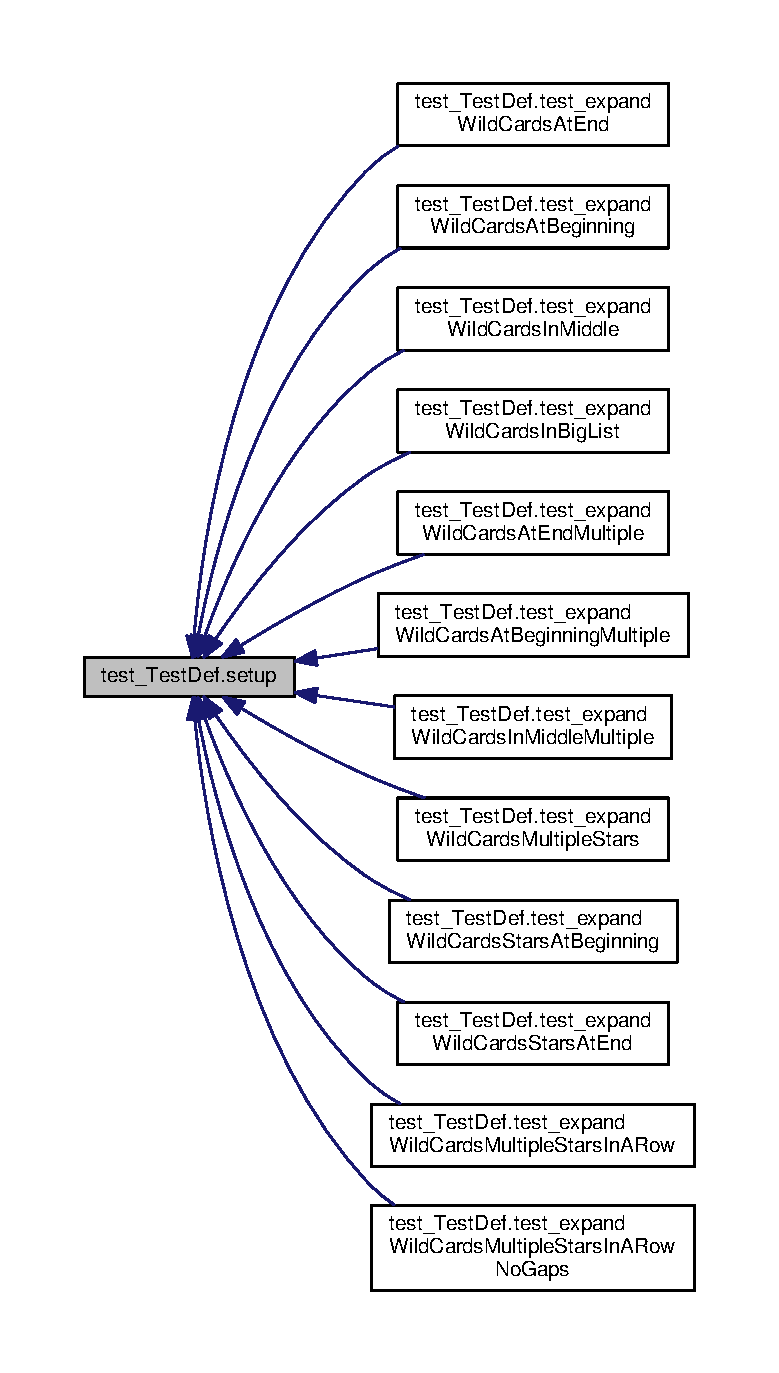
\includegraphics[height=550pt]{namespacetest___test_def_a5d6f39e8ce85a48a0ef17deef16256cf_icgraph}
\end{center}
\end{figure}


\hypertarget{namespacetest___test_def_ab07802efce3b4a7de2a14067c19e9360}{\index{test\-\_\-\-Test\-Def@{test\-\_\-\-Test\-Def}!test\-\_\-expand\-Wild\-Cards\-At\-Beginning@{test\-\_\-expand\-Wild\-Cards\-At\-Beginning}}
\index{test\-\_\-expand\-Wild\-Cards\-At\-Beginning@{test\-\_\-expand\-Wild\-Cards\-At\-Beginning}!test_TestDef@{test\-\_\-\-Test\-Def}}
\subsubsection[{test\-\_\-expand\-Wild\-Cards\-At\-Beginning}]{\setlength{\rightskip}{0pt plus 5cm}def test\-\_\-\-Test\-Def.\-test\-\_\-expand\-Wild\-Cards\-At\-Beginning (
\begin{DoxyParamCaption}
{}
\end{DoxyParamCaption}
)}}\label{namespacetest___test_def_ab07802efce3b4a7de2a14067c19e9360}


Definition at line 33 of file test\-\_\-\-Test\-Def.\-py.



Here is the call graph for this function\-:
\nopagebreak
\begin{figure}[H]
\begin{center}
\leavevmode
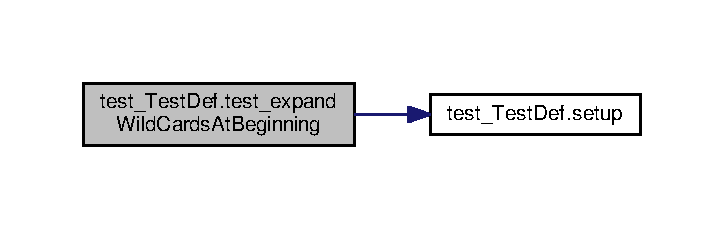
\includegraphics[width=348pt]{namespacetest___test_def_ab07802efce3b4a7de2a14067c19e9360_cgraph}
\end{center}
\end{figure}


\hypertarget{namespacetest___test_def_a7593fcb059257412f75feb9ee7e9112b}{\index{test\-\_\-\-Test\-Def@{test\-\_\-\-Test\-Def}!test\-\_\-expand\-Wild\-Cards\-At\-Beginning\-Multiple@{test\-\_\-expand\-Wild\-Cards\-At\-Beginning\-Multiple}}
\index{test\-\_\-expand\-Wild\-Cards\-At\-Beginning\-Multiple@{test\-\_\-expand\-Wild\-Cards\-At\-Beginning\-Multiple}!test_TestDef@{test\-\_\-\-Test\-Def}}
\subsubsection[{test\-\_\-expand\-Wild\-Cards\-At\-Beginning\-Multiple}]{\setlength{\rightskip}{0pt plus 5cm}def test\-\_\-\-Test\-Def.\-test\-\_\-expand\-Wild\-Cards\-At\-Beginning\-Multiple (
\begin{DoxyParamCaption}
{}
\end{DoxyParamCaption}
)}}\label{namespacetest___test_def_a7593fcb059257412f75feb9ee7e9112b}


Definition at line 81 of file test\-\_\-\-Test\-Def.\-py.



Here is the call graph for this function\-:
\nopagebreak
\begin{figure}[H]
\begin{center}
\leavevmode
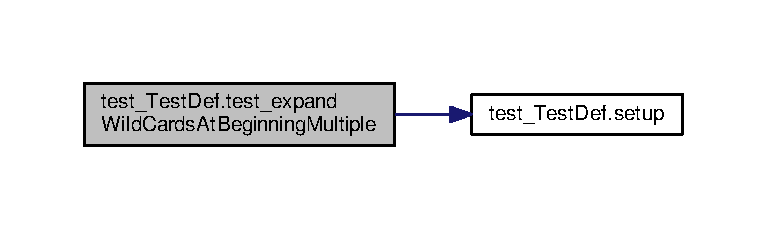
\includegraphics[width=350pt]{namespacetest___test_def_a7593fcb059257412f75feb9ee7e9112b_cgraph}
\end{center}
\end{figure}


\hypertarget{namespacetest___test_def_a1c975c41c4ea84398ab1f3c407086a2e}{\index{test\-\_\-\-Test\-Def@{test\-\_\-\-Test\-Def}!test\-\_\-expand\-Wild\-Cards\-At\-End@{test\-\_\-expand\-Wild\-Cards\-At\-End}}
\index{test\-\_\-expand\-Wild\-Cards\-At\-End@{test\-\_\-expand\-Wild\-Cards\-At\-End}!test_TestDef@{test\-\_\-\-Test\-Def}}
\subsubsection[{test\-\_\-expand\-Wild\-Cards\-At\-End}]{\setlength{\rightskip}{0pt plus 5cm}def test\-\_\-\-Test\-Def.\-test\-\_\-expand\-Wild\-Cards\-At\-End (
\begin{DoxyParamCaption}
{}
\end{DoxyParamCaption}
)}}\label{namespacetest___test_def_a1c975c41c4ea84398ab1f3c407086a2e}


Definition at line 22 of file test\-\_\-\-Test\-Def.\-py.



Here is the call graph for this function\-:
\nopagebreak
\begin{figure}[H]
\begin{center}
\leavevmode
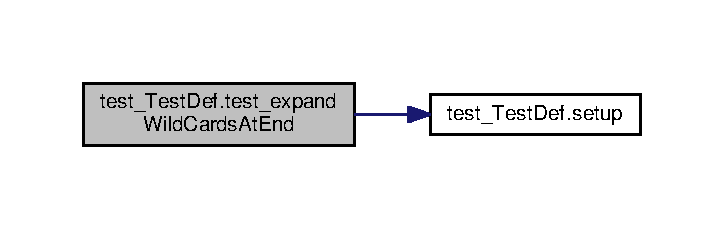
\includegraphics[width=348pt]{namespacetest___test_def_a1c975c41c4ea84398ab1f3c407086a2e_cgraph}
\end{center}
\end{figure}


\hypertarget{namespacetest___test_def_a7d4536413e9ff1d2c8e2ccce9408c1e0}{\index{test\-\_\-\-Test\-Def@{test\-\_\-\-Test\-Def}!test\-\_\-expand\-Wild\-Cards\-At\-End\-Multiple@{test\-\_\-expand\-Wild\-Cards\-At\-End\-Multiple}}
\index{test\-\_\-expand\-Wild\-Cards\-At\-End\-Multiple@{test\-\_\-expand\-Wild\-Cards\-At\-End\-Multiple}!test_TestDef@{test\-\_\-\-Test\-Def}}
\subsubsection[{test\-\_\-expand\-Wild\-Cards\-At\-End\-Multiple}]{\setlength{\rightskip}{0pt plus 5cm}def test\-\_\-\-Test\-Def.\-test\-\_\-expand\-Wild\-Cards\-At\-End\-Multiple (
\begin{DoxyParamCaption}
{}
\end{DoxyParamCaption}
)}}\label{namespacetest___test_def_a7d4536413e9ff1d2c8e2ccce9408c1e0}


Definition at line 68 of file test\-\_\-\-Test\-Def.\-py.



Here is the call graph for this function\-:
\nopagebreak
\begin{figure}[H]
\begin{center}
\leavevmode
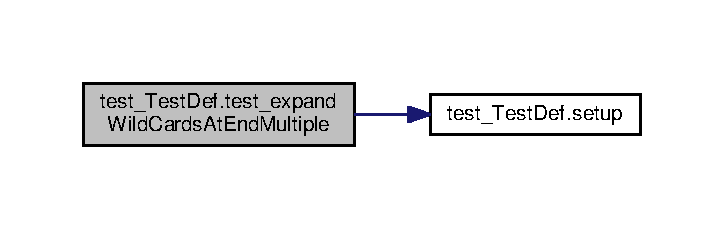
\includegraphics[width=348pt]{namespacetest___test_def_a7d4536413e9ff1d2c8e2ccce9408c1e0_cgraph}
\end{center}
\end{figure}


\hypertarget{namespacetest___test_def_a862e74186ada6ed014481a252a43e8d0}{\index{test\-\_\-\-Test\-Def@{test\-\_\-\-Test\-Def}!test\-\_\-expand\-Wild\-Cards\-In\-Big\-List@{test\-\_\-expand\-Wild\-Cards\-In\-Big\-List}}
\index{test\-\_\-expand\-Wild\-Cards\-In\-Big\-List@{test\-\_\-expand\-Wild\-Cards\-In\-Big\-List}!test_TestDef@{test\-\_\-\-Test\-Def}}
\subsubsection[{test\-\_\-expand\-Wild\-Cards\-In\-Big\-List}]{\setlength{\rightskip}{0pt plus 5cm}def test\-\_\-\-Test\-Def.\-test\-\_\-expand\-Wild\-Cards\-In\-Big\-List (
\begin{DoxyParamCaption}
{}
\end{DoxyParamCaption}
)}}\label{namespacetest___test_def_a862e74186ada6ed014481a252a43e8d0}


Definition at line 55 of file test\-\_\-\-Test\-Def.\-py.



Here is the call graph for this function\-:
\nopagebreak
\begin{figure}[H]
\begin{center}
\leavevmode
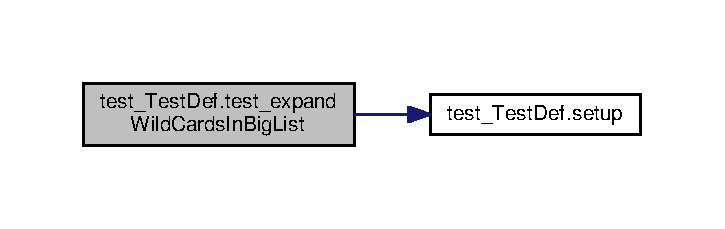
\includegraphics[width=348pt]{namespacetest___test_def_a862e74186ada6ed014481a252a43e8d0_cgraph}
\end{center}
\end{figure}


\hypertarget{namespacetest___test_def_a29ea2fb75922b7620bbe9bd2af164739}{\index{test\-\_\-\-Test\-Def@{test\-\_\-\-Test\-Def}!test\-\_\-expand\-Wild\-Cards\-In\-Middle@{test\-\_\-expand\-Wild\-Cards\-In\-Middle}}
\index{test\-\_\-expand\-Wild\-Cards\-In\-Middle@{test\-\_\-expand\-Wild\-Cards\-In\-Middle}!test_TestDef@{test\-\_\-\-Test\-Def}}
\subsubsection[{test\-\_\-expand\-Wild\-Cards\-In\-Middle}]{\setlength{\rightskip}{0pt plus 5cm}def test\-\_\-\-Test\-Def.\-test\-\_\-expand\-Wild\-Cards\-In\-Middle (
\begin{DoxyParamCaption}
{}
\end{DoxyParamCaption}
)}}\label{namespacetest___test_def_a29ea2fb75922b7620bbe9bd2af164739}


Definition at line 44 of file test\-\_\-\-Test\-Def.\-py.



Here is the call graph for this function\-:
\nopagebreak
\begin{figure}[H]
\begin{center}
\leavevmode
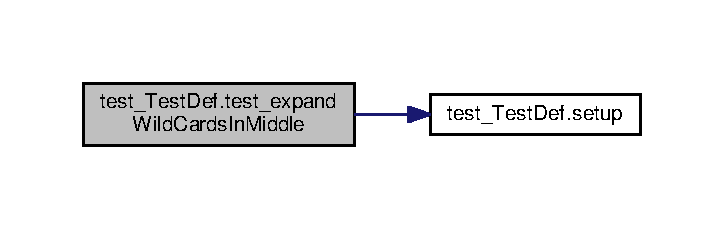
\includegraphics[width=348pt]{namespacetest___test_def_a29ea2fb75922b7620bbe9bd2af164739_cgraph}
\end{center}
\end{figure}


\hypertarget{namespacetest___test_def_ad4def05d16a3b403fdeafd125d7e91e7}{\index{test\-\_\-\-Test\-Def@{test\-\_\-\-Test\-Def}!test\-\_\-expand\-Wild\-Cards\-In\-Middle\-Multiple@{test\-\_\-expand\-Wild\-Cards\-In\-Middle\-Multiple}}
\index{test\-\_\-expand\-Wild\-Cards\-In\-Middle\-Multiple@{test\-\_\-expand\-Wild\-Cards\-In\-Middle\-Multiple}!test_TestDef@{test\-\_\-\-Test\-Def}}
\subsubsection[{test\-\_\-expand\-Wild\-Cards\-In\-Middle\-Multiple}]{\setlength{\rightskip}{0pt plus 5cm}def test\-\_\-\-Test\-Def.\-test\-\_\-expand\-Wild\-Cards\-In\-Middle\-Multiple (
\begin{DoxyParamCaption}
{}
\end{DoxyParamCaption}
)}}\label{namespacetest___test_def_ad4def05d16a3b403fdeafd125d7e91e7}


Definition at line 94 of file test\-\_\-\-Test\-Def.\-py.



Here is the call graph for this function\-:
\nopagebreak
\begin{figure}[H]
\begin{center}
\leavevmode
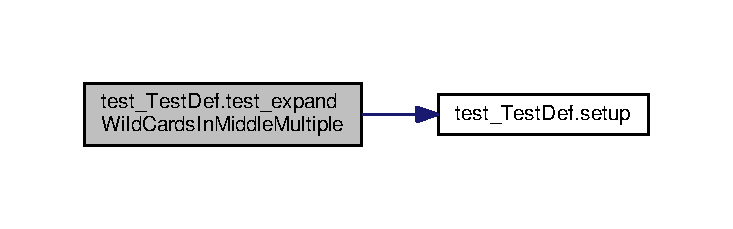
\includegraphics[width=350pt]{namespacetest___test_def_ad4def05d16a3b403fdeafd125d7e91e7_cgraph}
\end{center}
\end{figure}


\hypertarget{namespacetest___test_def_a912242120ad4887ab854ce51620040a9}{\index{test\-\_\-\-Test\-Def@{test\-\_\-\-Test\-Def}!test\-\_\-expand\-Wild\-Cards\-Multiple\-Stars@{test\-\_\-expand\-Wild\-Cards\-Multiple\-Stars}}
\index{test\-\_\-expand\-Wild\-Cards\-Multiple\-Stars@{test\-\_\-expand\-Wild\-Cards\-Multiple\-Stars}!test_TestDef@{test\-\_\-\-Test\-Def}}
\subsubsection[{test\-\_\-expand\-Wild\-Cards\-Multiple\-Stars}]{\setlength{\rightskip}{0pt plus 5cm}def test\-\_\-\-Test\-Def.\-test\-\_\-expand\-Wild\-Cards\-Multiple\-Stars (
\begin{DoxyParamCaption}
{}
\end{DoxyParamCaption}
)}}\label{namespacetest___test_def_a912242120ad4887ab854ce51620040a9}


Definition at line 107 of file test\-\_\-\-Test\-Def.\-py.



Here is the call graph for this function\-:
\nopagebreak
\begin{figure}[H]
\begin{center}
\leavevmode
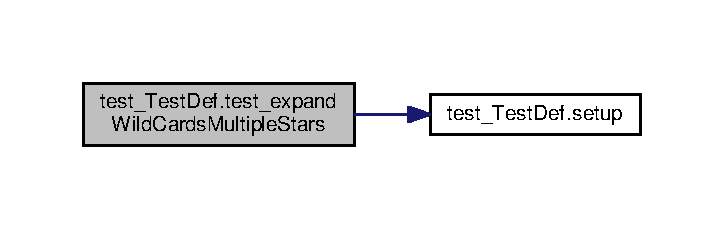
\includegraphics[width=348pt]{namespacetest___test_def_a912242120ad4887ab854ce51620040a9_cgraph}
\end{center}
\end{figure}


\hypertarget{namespacetest___test_def_aec3b4133f1e46fa5b3042e3d1419cde3}{\index{test\-\_\-\-Test\-Def@{test\-\_\-\-Test\-Def}!test\-\_\-expand\-Wild\-Cards\-Multiple\-Stars\-In\-A\-Row@{test\-\_\-expand\-Wild\-Cards\-Multiple\-Stars\-In\-A\-Row}}
\index{test\-\_\-expand\-Wild\-Cards\-Multiple\-Stars\-In\-A\-Row@{test\-\_\-expand\-Wild\-Cards\-Multiple\-Stars\-In\-A\-Row}!test_TestDef@{test\-\_\-\-Test\-Def}}
\subsubsection[{test\-\_\-expand\-Wild\-Cards\-Multiple\-Stars\-In\-A\-Row}]{\setlength{\rightskip}{0pt plus 5cm}def test\-\_\-\-Test\-Def.\-test\-\_\-expand\-Wild\-Cards\-Multiple\-Stars\-In\-A\-Row (
\begin{DoxyParamCaption}
{}
\end{DoxyParamCaption}
)}}\label{namespacetest___test_def_aec3b4133f1e46fa5b3042e3d1419cde3}


Definition at line 158 of file test\-\_\-\-Test\-Def.\-py.



Here is the call graph for this function\-:
\nopagebreak
\begin{figure}[H]
\begin{center}
\leavevmode
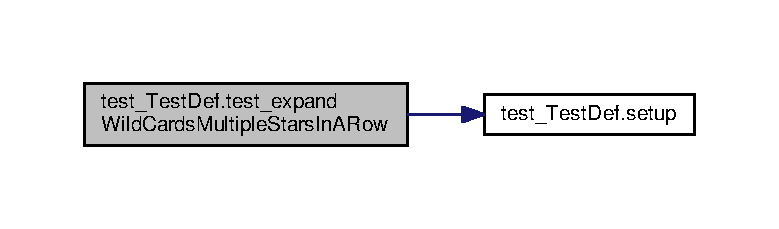
\includegraphics[width=350pt]{namespacetest___test_def_aec3b4133f1e46fa5b3042e3d1419cde3_cgraph}
\end{center}
\end{figure}


\hypertarget{namespacetest___test_def_a8fc79791143e851ce5a852c5f443dc67}{\index{test\-\_\-\-Test\-Def@{test\-\_\-\-Test\-Def}!test\-\_\-expand\-Wild\-Cards\-Multiple\-Stars\-In\-A\-Row\-No\-Gaps@{test\-\_\-expand\-Wild\-Cards\-Multiple\-Stars\-In\-A\-Row\-No\-Gaps}}
\index{test\-\_\-expand\-Wild\-Cards\-Multiple\-Stars\-In\-A\-Row\-No\-Gaps@{test\-\_\-expand\-Wild\-Cards\-Multiple\-Stars\-In\-A\-Row\-No\-Gaps}!test_TestDef@{test\-\_\-\-Test\-Def}}
\subsubsection[{test\-\_\-expand\-Wild\-Cards\-Multiple\-Stars\-In\-A\-Row\-No\-Gaps}]{\setlength{\rightskip}{0pt plus 5cm}def test\-\_\-\-Test\-Def.\-test\-\_\-expand\-Wild\-Cards\-Multiple\-Stars\-In\-A\-Row\-No\-Gaps (
\begin{DoxyParamCaption}
{}
\end{DoxyParamCaption}
)}}\label{namespacetest___test_def_a8fc79791143e851ce5a852c5f443dc67}


Definition at line 169 of file test\-\_\-\-Test\-Def.\-py.



Here is the call graph for this function\-:
\nopagebreak
\begin{figure}[H]
\begin{center}
\leavevmode
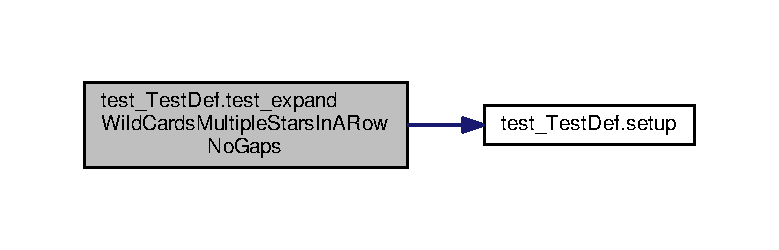
\includegraphics[width=350pt]{namespacetest___test_def_a8fc79791143e851ce5a852c5f443dc67_cgraph}
\end{center}
\end{figure}


\hypertarget{namespacetest___test_def_a7ddfa88efe8536ca1c1cff0e51567593}{\index{test\-\_\-\-Test\-Def@{test\-\_\-\-Test\-Def}!test\-\_\-expand\-Wild\-Cards\-Stars\-At\-Beginning@{test\-\_\-expand\-Wild\-Cards\-Stars\-At\-Beginning}}
\index{test\-\_\-expand\-Wild\-Cards\-Stars\-At\-Beginning@{test\-\_\-expand\-Wild\-Cards\-Stars\-At\-Beginning}!test_TestDef@{test\-\_\-\-Test\-Def}}
\subsubsection[{test\-\_\-expand\-Wild\-Cards\-Stars\-At\-Beginning}]{\setlength{\rightskip}{0pt plus 5cm}def test\-\_\-\-Test\-Def.\-test\-\_\-expand\-Wild\-Cards\-Stars\-At\-Beginning (
\begin{DoxyParamCaption}
{}
\end{DoxyParamCaption}
)}}\label{namespacetest___test_def_a7ddfa88efe8536ca1c1cff0e51567593}


Definition at line 120 of file test\-\_\-\-Test\-Def.\-py.



Here is the call graph for this function\-:
\nopagebreak
\begin{figure}[H]
\begin{center}
\leavevmode
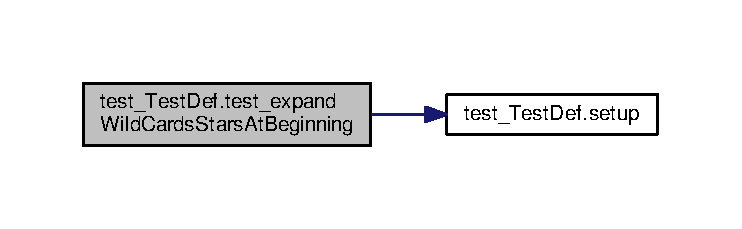
\includegraphics[width=350pt]{namespacetest___test_def_a7ddfa88efe8536ca1c1cff0e51567593_cgraph}
\end{center}
\end{figure}


\hypertarget{namespacetest___test_def_a4b3d40e5bede74b30308a467da9d2018}{\index{test\-\_\-\-Test\-Def@{test\-\_\-\-Test\-Def}!test\-\_\-expand\-Wild\-Cards\-Stars\-At\-End@{test\-\_\-expand\-Wild\-Cards\-Stars\-At\-End}}
\index{test\-\_\-expand\-Wild\-Cards\-Stars\-At\-End@{test\-\_\-expand\-Wild\-Cards\-Stars\-At\-End}!test_TestDef@{test\-\_\-\-Test\-Def}}
\subsubsection[{test\-\_\-expand\-Wild\-Cards\-Stars\-At\-End}]{\setlength{\rightskip}{0pt plus 5cm}def test\-\_\-\-Test\-Def.\-test\-\_\-expand\-Wild\-Cards\-Stars\-At\-End (
\begin{DoxyParamCaption}
{}
\end{DoxyParamCaption}
)}}\label{namespacetest___test_def_a4b3d40e5bede74b30308a467da9d2018}


Definition at line 133 of file test\-\_\-\-Test\-Def.\-py.



Here is the call graph for this function\-:
\nopagebreak
\begin{figure}[H]
\begin{center}
\leavevmode
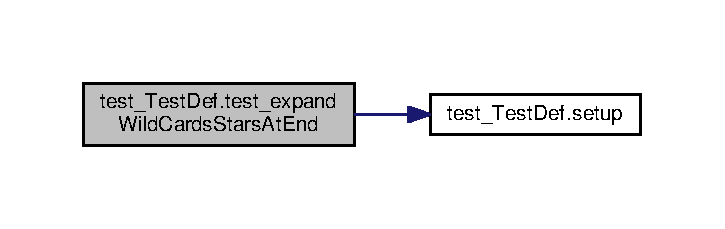
\includegraphics[width=348pt]{namespacetest___test_def_a4b3d40e5bede74b30308a467da9d2018_cgraph}
\end{center}
\end{figure}



\hypertarget{namespace_test_build_m_t_t_stage}{\section{Test\-Build\-M\-T\-T\-Stage Namespace Reference}
\label{namespace_test_build_m_t_t_stage}\index{Test\-Build\-M\-T\-T\-Stage@{Test\-Build\-M\-T\-T\-Stage}}
}
\subsection*{Classes}
\begin{DoxyCompactItemize}
\item 
class \hyperlink{class_test_build_m_t_t_stage_1_1_test_build_m_t_t_stage}{Test\-Build\-M\-T\-T\-Stage}
\end{DoxyCompactItemize}

\hypertarget{namespace_test_def}{\section{Test\-Def Namespace Reference}
\label{namespace_test_def}\index{Test\-Def@{Test\-Def}}
}
\subsection*{Classes}
\begin{DoxyCompactItemize}
\item 
class \hyperlink{class_test_def_1_1_test_def}{Test\-Def}
\end{DoxyCompactItemize}
\subsection*{Functions}
\begin{DoxyCompactItemize}
\item 
def \hyperlink{namespace_test_def_a0f44619ec0fe932324e50d8cf706d647}{\-\_\-mkdir\-\_\-recursive}
\end{DoxyCompactItemize}
\subsection*{Variables}
\begin{DoxyCompactItemize}
\item 
list \hyperlink{namespace_test_def_a4e87724b7a6a117c2cca22c557936868}{is\-\_\-py2} = sys.\-version\mbox{[}0\mbox{]}
\end{DoxyCompactItemize}


\subsection{Function Documentation}
\hypertarget{namespace_test_def_a0f44619ec0fe932324e50d8cf706d647}{\index{Test\-Def@{Test\-Def}!\-\_\-mkdir\-\_\-recursive@{\-\_\-mkdir\-\_\-recursive}}
\index{\-\_\-mkdir\-\_\-recursive@{\-\_\-mkdir\-\_\-recursive}!TestDef@{Test\-Def}}
\subsubsection[{\-\_\-mkdir\-\_\-recursive}]{\setlength{\rightskip}{0pt plus 5cm}def Test\-Def.\-\_\-mkdir\-\_\-recursive (
\begin{DoxyParamCaption}
\item[{}]{path}
\end{DoxyParamCaption}
)\hspace{0.3cm}{\ttfamily [private]}}}\label{namespace_test_def_a0f44619ec0fe932324e50d8cf706d647}


Definition at line 35 of file Test\-Def.\-py.



\subsection{Variable Documentation}
\hypertarget{namespace_test_def_a4e87724b7a6a117c2cca22c557936868}{\index{Test\-Def@{Test\-Def}!is\-\_\-py2@{is\-\_\-py2}}
\index{is\-\_\-py2@{is\-\_\-py2}!TestDef@{Test\-Def}}
\subsubsection[{is\-\_\-py2}]{\setlength{\rightskip}{0pt plus 5cm}list Test\-Def.\-is\-\_\-py2 = sys.\-version\mbox{[}0\mbox{]}}}\label{namespace_test_def_a4e87724b7a6a117c2cca22c557936868}


Definition at line 29 of file Test\-Def.\-py.


\hypertarget{namespace_test_get_m_t_t_stage}{\section{Test\-Get\-M\-T\-T\-Stage Namespace Reference}
\label{namespace_test_get_m_t_t_stage}\index{Test\-Get\-M\-T\-T\-Stage@{Test\-Get\-M\-T\-T\-Stage}}
}
\subsection*{Classes}
\begin{DoxyCompactItemize}
\item 
class \hyperlink{class_test_get_m_t_t_stage_1_1_test_get_m_t_t_stage}{Test\-Get\-M\-T\-T\-Stage}
\end{DoxyCompactItemize}

\hypertarget{namespace_test_run_m_t_t_stage}{\section{Test\-Run\-M\-T\-T\-Stage Namespace Reference}
\label{namespace_test_run_m_t_t_stage}\index{Test\-Run\-M\-T\-T\-Stage@{Test\-Run\-M\-T\-T\-Stage}}
}
\subsection*{Classes}
\begin{DoxyCompactItemize}
\item 
class \hyperlink{class_test_run_m_t_t_stage_1_1_test_run_m_t_t_stage}{Test\-Run\-M\-T\-T\-Stage}
\end{DoxyCompactItemize}

\hypertarget{namespace_text_file}{\section{Text\-File Namespace Reference}
\label{namespace_text_file}\index{Text\-File@{Text\-File}}
}
\subsection*{Classes}
\begin{DoxyCompactItemize}
\item 
class \hyperlink{class_text_file_1_1_text_file}{Text\-File}
\end{DoxyCompactItemize}

\hypertarget{namespace_version_m_t_t_tool}{\section{Version\-M\-T\-T\-Tool Namespace Reference}
\label{namespace_version_m_t_t_tool}\index{Version\-M\-T\-T\-Tool@{Version\-M\-T\-T\-Tool}}
}
\subsection*{Classes}
\begin{DoxyCompactItemize}
\item 
class \hyperlink{class_version_m_t_t_tool_1_1_version_m_t_t_tool}{Version\-M\-T\-T\-Tool}
\end{DoxyCompactItemize}

\hypertarget{namespace_watchdog}{\section{Watchdog Namespace Reference}
\label{namespace_watchdog}\index{Watchdog@{Watchdog}}
}
\subsection*{Classes}
\begin{DoxyCompactItemize}
\item 
class \hyperlink{class_watchdog_1_1_watchdog}{Watchdog}
\end{DoxyCompactItemize}

\hypertarget{namespace_w_wulf3}{\section{W\-Wulf3 Namespace Reference}
\label{namespace_w_wulf3}\index{W\-Wulf3@{W\-Wulf3}}
}
\subsection*{Classes}
\begin{DoxyCompactItemize}
\item 
class \hyperlink{class_w_wulf3_1_1_w_wulf3}{W\-Wulf3}
\end{DoxyCompactItemize}

\chapter{Class Documentation}
\hypertarget{class_a_l_p_s_1_1_a_l_p_s}{\section{A\-L\-P\-S.\-A\-L\-P\-S Class Reference}
\label{class_a_l_p_s_1_1_a_l_p_s}\index{A\-L\-P\-S.\-A\-L\-P\-S@{A\-L\-P\-S.\-A\-L\-P\-S}}
}


Inheritance diagram for A\-L\-P\-S.\-A\-L\-P\-S\-:
\nopagebreak
\begin{figure}[H]
\begin{center}
\leavevmode
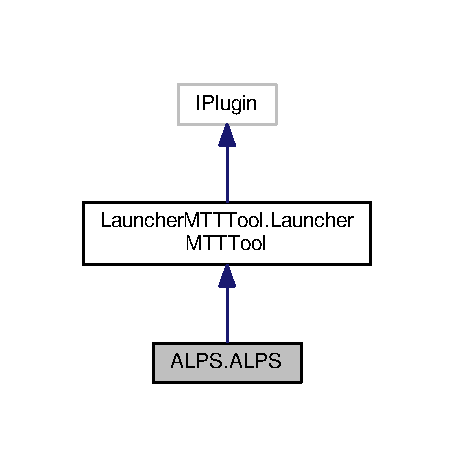
\includegraphics[width=218pt]{class_a_l_p_s_1_1_a_l_p_s__inherit__graph}
\end{center}
\end{figure}


Collaboration diagram for A\-L\-P\-S.\-A\-L\-P\-S\-:
\nopagebreak
\begin{figure}[H]
\begin{center}
\leavevmode
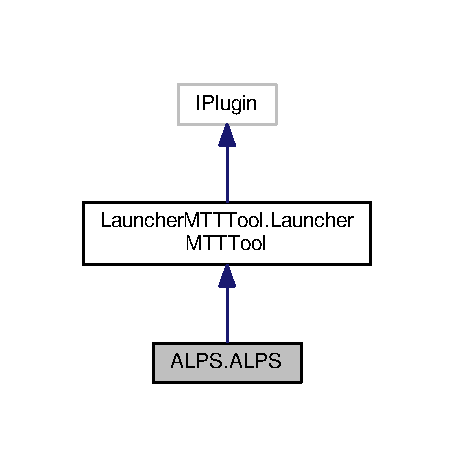
\includegraphics[width=218pt]{class_a_l_p_s_1_1_a_l_p_s__coll__graph}
\end{center}
\end{figure}
\subsection*{Public Member Functions}
\begin{DoxyCompactItemize}
\item 
def \hyperlink{class_a_l_p_s_1_1_a_l_p_s_a45417f6290435c66b3f3b7c4586915d9}{\-\_\-\-\_\-init\-\_\-\-\_\-}
\item 
def \hyperlink{class_a_l_p_s_1_1_a_l_p_s_a3d507bd3feb505c8ed1b4e8f3729d636}{activate}
\item 
def \hyperlink{class_a_l_p_s_1_1_a_l_p_s_aa1d63291a23bcca8ccbd44dc4d0fa6bf}{deactivate}
\item 
def \hyperlink{class_a_l_p_s_1_1_a_l_p_s_a97e56ee7f5faaea26121d6ee0deeddab}{print\-\_\-name}
\item 
def \hyperlink{class_a_l_p_s_1_1_a_l_p_s_a68c17d876ad850e44d40aa082b674f4e}{print\-\_\-options}
\item 
def \hyperlink{class_a_l_p_s_1_1_a_l_p_s_af4b8efc64ea3abc5fb21fb93bfe052ff}{execute}
\end{DoxyCompactItemize}
\subsection*{Public Attributes}
\begin{DoxyCompactItemize}
\item 
\hyperlink{class_a_l_p_s_1_1_a_l_p_s_a24dfa9b508f507c4cb6148f10a081555}{options}
\item 
\hyperlink{class_a_l_p_s_1_1_a_l_p_s_ac371dce53e8c120f7031259025562bdb}{allocated}
\item 
\hyperlink{class_a_l_p_s_1_1_a_l_p_s_a839c4f84a46683221d51004c08345ff2}{test\-Def}
\item 
\hyperlink{class_a_l_p_s_1_1_a_l_p_s_a64bae95ba692ef4df06f716692b50ee9}{cmds}
\end{DoxyCompactItemize}


\subsection{Detailed Description}


Definition at line 41 of file A\-L\-P\-S.\-py.



\subsection{Constructor \& Destructor Documentation}
\hypertarget{class_a_l_p_s_1_1_a_l_p_s_a45417f6290435c66b3f3b7c4586915d9}{\index{A\-L\-P\-S\-::\-A\-L\-P\-S@{A\-L\-P\-S\-::\-A\-L\-P\-S}!\-\_\-\-\_\-init\-\_\-\-\_\-@{\-\_\-\-\_\-init\-\_\-\-\_\-}}
\index{\-\_\-\-\_\-init\-\_\-\-\_\-@{\-\_\-\-\_\-init\-\_\-\-\_\-}!ALPS::ALPS@{A\-L\-P\-S\-::\-A\-L\-P\-S}}
\subsubsection[{\-\_\-\-\_\-init\-\_\-\-\_\-}]{\setlength{\rightskip}{0pt plus 5cm}def A\-L\-P\-S.\-A\-L\-P\-S.\-\_\-\-\_\-init\-\_\-\-\_\- (
\begin{DoxyParamCaption}
\item[{}]{self}
\end{DoxyParamCaption}
)}}\label{class_a_l_p_s_1_1_a_l_p_s_a45417f6290435c66b3f3b7c4586915d9}


Definition at line 43 of file A\-L\-P\-S.\-py.



\subsection{Member Function Documentation}
\hypertarget{class_a_l_p_s_1_1_a_l_p_s_a3d507bd3feb505c8ed1b4e8f3729d636}{\index{A\-L\-P\-S\-::\-A\-L\-P\-S@{A\-L\-P\-S\-::\-A\-L\-P\-S}!activate@{activate}}
\index{activate@{activate}!ALPS::ALPS@{A\-L\-P\-S\-::\-A\-L\-P\-S}}
\subsubsection[{activate}]{\setlength{\rightskip}{0pt plus 5cm}def A\-L\-P\-S.\-A\-L\-P\-S.\-activate (
\begin{DoxyParamCaption}
\item[{}]{self}
\end{DoxyParamCaption}
)}}\label{class_a_l_p_s_1_1_a_l_p_s_a3d507bd3feb505c8ed1b4e8f3729d636}


Definition at line 73 of file A\-L\-P\-S.\-py.

\hypertarget{class_a_l_p_s_1_1_a_l_p_s_aa1d63291a23bcca8ccbd44dc4d0fa6bf}{\index{A\-L\-P\-S\-::\-A\-L\-P\-S@{A\-L\-P\-S\-::\-A\-L\-P\-S}!deactivate@{deactivate}}
\index{deactivate@{deactivate}!ALPS::ALPS@{A\-L\-P\-S\-::\-A\-L\-P\-S}}
\subsubsection[{deactivate}]{\setlength{\rightskip}{0pt plus 5cm}def A\-L\-P\-S.\-A\-L\-P\-S.\-deactivate (
\begin{DoxyParamCaption}
\item[{}]{self}
\end{DoxyParamCaption}
)}}\label{class_a_l_p_s_1_1_a_l_p_s_aa1d63291a23bcca8ccbd44dc4d0fa6bf}


Definition at line 79 of file A\-L\-P\-S.\-py.

\hypertarget{class_a_l_p_s_1_1_a_l_p_s_af4b8efc64ea3abc5fb21fb93bfe052ff}{\index{A\-L\-P\-S\-::\-A\-L\-P\-S@{A\-L\-P\-S\-::\-A\-L\-P\-S}!execute@{execute}}
\index{execute@{execute}!ALPS::ALPS@{A\-L\-P\-S\-::\-A\-L\-P\-S}}
\subsubsection[{execute}]{\setlength{\rightskip}{0pt plus 5cm}def A\-L\-P\-S.\-A\-L\-P\-S.\-execute (
\begin{DoxyParamCaption}
\item[{}]{self, }
\item[{}]{log, }
\item[{}]{keyvals, }
\item[{}]{test\-Def}
\end{DoxyParamCaption}
)}}\label{class_a_l_p_s_1_1_a_l_p_s_af4b8efc64ea3abc5fb21fb93bfe052ff}


Definition at line 96 of file A\-L\-P\-S.\-py.

\hypertarget{class_a_l_p_s_1_1_a_l_p_s_a97e56ee7f5faaea26121d6ee0deeddab}{\index{A\-L\-P\-S\-::\-A\-L\-P\-S@{A\-L\-P\-S\-::\-A\-L\-P\-S}!print\-\_\-name@{print\-\_\-name}}
\index{print\-\_\-name@{print\-\_\-name}!ALPS::ALPS@{A\-L\-P\-S\-::\-A\-L\-P\-S}}
\subsubsection[{print\-\_\-name}]{\setlength{\rightskip}{0pt plus 5cm}def A\-L\-P\-S.\-A\-L\-P\-S.\-print\-\_\-name (
\begin{DoxyParamCaption}
\item[{}]{self}
\end{DoxyParamCaption}
)}}\label{class_a_l_p_s_1_1_a_l_p_s_a97e56ee7f5faaea26121d6ee0deeddab}


Definition at line 87 of file A\-L\-P\-S.\-py.

\hypertarget{class_a_l_p_s_1_1_a_l_p_s_a68c17d876ad850e44d40aa082b674f4e}{\index{A\-L\-P\-S\-::\-A\-L\-P\-S@{A\-L\-P\-S\-::\-A\-L\-P\-S}!print\-\_\-options@{print\-\_\-options}}
\index{print\-\_\-options@{print\-\_\-options}!ALPS::ALPS@{A\-L\-P\-S\-::\-A\-L\-P\-S}}
\subsubsection[{print\-\_\-options}]{\setlength{\rightskip}{0pt plus 5cm}def A\-L\-P\-S.\-A\-L\-P\-S.\-print\-\_\-options (
\begin{DoxyParamCaption}
\item[{}]{self, }
\item[{}]{test\-Def, }
\item[{}]{prefix}
\end{DoxyParamCaption}
)}}\label{class_a_l_p_s_1_1_a_l_p_s_a68c17d876ad850e44d40aa082b674f4e}


Definition at line 90 of file A\-L\-P\-S.\-py.



\subsection{Member Data Documentation}
\hypertarget{class_a_l_p_s_1_1_a_l_p_s_ac371dce53e8c120f7031259025562bdb}{\index{A\-L\-P\-S\-::\-A\-L\-P\-S@{A\-L\-P\-S\-::\-A\-L\-P\-S}!allocated@{allocated}}
\index{allocated@{allocated}!ALPS::ALPS@{A\-L\-P\-S\-::\-A\-L\-P\-S}}
\subsubsection[{allocated}]{\setlength{\rightskip}{0pt plus 5cm}A\-L\-P\-S.\-A\-L\-P\-S.\-allocated}}\label{class_a_l_p_s_1_1_a_l_p_s_ac371dce53e8c120f7031259025562bdb}


Definition at line 67 of file A\-L\-P\-S.\-py.

\hypertarget{class_a_l_p_s_1_1_a_l_p_s_a64bae95ba692ef4df06f716692b50ee9}{\index{A\-L\-P\-S\-::\-A\-L\-P\-S@{A\-L\-P\-S\-::\-A\-L\-P\-S}!cmds@{cmds}}
\index{cmds@{cmds}!ALPS::ALPS@{A\-L\-P\-S\-::\-A\-L\-P\-S}}
\subsubsection[{cmds}]{\setlength{\rightskip}{0pt plus 5cm}A\-L\-P\-S.\-A\-L\-P\-S.\-cmds}}\label{class_a_l_p_s_1_1_a_l_p_s_a64bae95ba692ef4df06f716692b50ee9}


Definition at line 69 of file A\-L\-P\-S.\-py.

\hypertarget{class_a_l_p_s_1_1_a_l_p_s_a24dfa9b508f507c4cb6148f10a081555}{\index{A\-L\-P\-S\-::\-A\-L\-P\-S@{A\-L\-P\-S\-::\-A\-L\-P\-S}!options@{options}}
\index{options@{options}!ALPS::ALPS@{A\-L\-P\-S\-::\-A\-L\-P\-S}}
\subsubsection[{options}]{\setlength{\rightskip}{0pt plus 5cm}A\-L\-P\-S.\-A\-L\-P\-S.\-options}}\label{class_a_l_p_s_1_1_a_l_p_s_a24dfa9b508f507c4cb6148f10a081555}


Definition at line 46 of file A\-L\-P\-S.\-py.

\hypertarget{class_a_l_p_s_1_1_a_l_p_s_a839c4f84a46683221d51004c08345ff2}{\index{A\-L\-P\-S\-::\-A\-L\-P\-S@{A\-L\-P\-S\-::\-A\-L\-P\-S}!test\-Def@{test\-Def}}
\index{test\-Def@{test\-Def}!ALPS::ALPS@{A\-L\-P\-S\-::\-A\-L\-P\-S}}
\subsubsection[{test\-Def}]{\setlength{\rightskip}{0pt plus 5cm}A\-L\-P\-S.\-A\-L\-P\-S.\-test\-Def}}\label{class_a_l_p_s_1_1_a_l_p_s_a839c4f84a46683221d51004c08345ff2}


Definition at line 68 of file A\-L\-P\-S.\-py.



The documentation for this class was generated from the following file\-:\begin{DoxyCompactItemize}
\item 
/home/travis/build/open-\/mpi/mtt/pylib/\-Tools/\-Launcher/\hyperlink{_a_l_p_s_8py}{A\-L\-P\-S.\-py}\end{DoxyCompactItemize}

\hypertarget{class_already_installed_1_1_already_installed}{\section{Already\-Installed.\-Already\-Installed Class Reference}
\label{class_already_installed_1_1_already_installed}\index{Already\-Installed.\-Already\-Installed@{Already\-Installed.\-Already\-Installed}}
}


Inheritance diagram for Already\-Installed.\-Already\-Installed\-:
\nopagebreak
\begin{figure}[H]
\begin{center}
\leavevmode
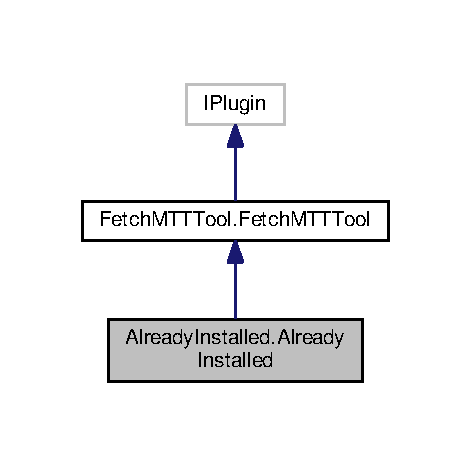
\includegraphics[width=226pt]{class_already_installed_1_1_already_installed__inherit__graph}
\end{center}
\end{figure}


Collaboration diagram for Already\-Installed.\-Already\-Installed\-:
\nopagebreak
\begin{figure}[H]
\begin{center}
\leavevmode
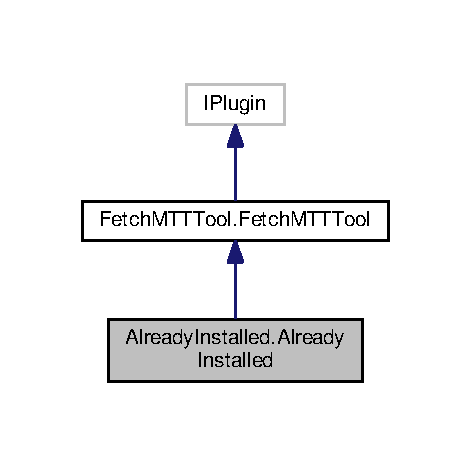
\includegraphics[width=226pt]{class_already_installed_1_1_already_installed__coll__graph}
\end{center}
\end{figure}
\subsection*{Public Member Functions}
\begin{DoxyCompactItemize}
\item 
def \hyperlink{class_already_installed_1_1_already_installed_ad412a2ca55660bde9d102ffffea5685f}{\-\_\-\-\_\-init\-\_\-\-\_\-}
\item 
def \hyperlink{class_already_installed_1_1_already_installed_aa69327b411af4bc2cd43f2bbf07cfe56}{activate}
\item 
def \hyperlink{class_already_installed_1_1_already_installed_a895aa66471ba8b5d4f67f8d17df5131c}{deactivate}
\item 
def \hyperlink{class_already_installed_1_1_already_installed_a63ce43492cf6c53f23a19a444109bfa8}{print\-\_\-name}
\item 
def \hyperlink{class_already_installed_1_1_already_installed_a8061d145324dbf058b17bc16579e9d5f}{print\-\_\-options}
\item 
def \hyperlink{class_already_installed_1_1_already_installed_af1afb26d21ce30a80e68c834245baeda}{execute}
\end{DoxyCompactItemize}
\subsection*{Public Attributes}
\begin{DoxyCompactItemize}
\item 
\hyperlink{class_already_installed_1_1_already_installed_af9247ff7a3b5dab409644868b7cc34e3}{options}
\end{DoxyCompactItemize}


\subsection{Detailed Description}


Definition at line 24 of file Already\-Installed.\-py.



\subsection{Constructor \& Destructor Documentation}
\hypertarget{class_already_installed_1_1_already_installed_ad412a2ca55660bde9d102ffffea5685f}{\index{Already\-Installed\-::\-Already\-Installed@{Already\-Installed\-::\-Already\-Installed}!\-\_\-\-\_\-init\-\_\-\-\_\-@{\-\_\-\-\_\-init\-\_\-\-\_\-}}
\index{\-\_\-\-\_\-init\-\_\-\-\_\-@{\-\_\-\-\_\-init\-\_\-\-\_\-}!AlreadyInstalled::AlreadyInstalled@{Already\-Installed\-::\-Already\-Installed}}
\subsubsection[{\-\_\-\-\_\-init\-\_\-\-\_\-}]{\setlength{\rightskip}{0pt plus 5cm}def Already\-Installed.\-Already\-Installed.\-\_\-\-\_\-init\-\_\-\-\_\- (
\begin{DoxyParamCaption}
\item[{}]{self}
\end{DoxyParamCaption}
)}}\label{class_already_installed_1_1_already_installed_ad412a2ca55660bde9d102ffffea5685f}


Definition at line 26 of file Already\-Installed.\-py.



\subsection{Member Function Documentation}
\hypertarget{class_already_installed_1_1_already_installed_aa69327b411af4bc2cd43f2bbf07cfe56}{\index{Already\-Installed\-::\-Already\-Installed@{Already\-Installed\-::\-Already\-Installed}!activate@{activate}}
\index{activate@{activate}!AlreadyInstalled::AlreadyInstalled@{Already\-Installed\-::\-Already\-Installed}}
\subsubsection[{activate}]{\setlength{\rightskip}{0pt plus 5cm}def Already\-Installed.\-Already\-Installed.\-activate (
\begin{DoxyParamCaption}
\item[{}]{self}
\end{DoxyParamCaption}
)}}\label{class_already_installed_1_1_already_installed_aa69327b411af4bc2cd43f2bbf07cfe56}


Definition at line 34 of file Already\-Installed.\-py.

\hypertarget{class_already_installed_1_1_already_installed_a895aa66471ba8b5d4f67f8d17df5131c}{\index{Already\-Installed\-::\-Already\-Installed@{Already\-Installed\-::\-Already\-Installed}!deactivate@{deactivate}}
\index{deactivate@{deactivate}!AlreadyInstalled::AlreadyInstalled@{Already\-Installed\-::\-Already\-Installed}}
\subsubsection[{deactivate}]{\setlength{\rightskip}{0pt plus 5cm}def Already\-Installed.\-Already\-Installed.\-deactivate (
\begin{DoxyParamCaption}
\item[{}]{self}
\end{DoxyParamCaption}
)}}\label{class_already_installed_1_1_already_installed_a895aa66471ba8b5d4f67f8d17df5131c}


Definition at line 40 of file Already\-Installed.\-py.

\hypertarget{class_already_installed_1_1_already_installed_af1afb26d21ce30a80e68c834245baeda}{\index{Already\-Installed\-::\-Already\-Installed@{Already\-Installed\-::\-Already\-Installed}!execute@{execute}}
\index{execute@{execute}!AlreadyInstalled::AlreadyInstalled@{Already\-Installed\-::\-Already\-Installed}}
\subsubsection[{execute}]{\setlength{\rightskip}{0pt plus 5cm}def Already\-Installed.\-Already\-Installed.\-execute (
\begin{DoxyParamCaption}
\item[{}]{self, }
\item[{}]{log, }
\item[{}]{keyvals, }
\item[{}]{test\-Def}
\end{DoxyParamCaption}
)}}\label{class_already_installed_1_1_already_installed_af1afb26d21ce30a80e68c834245baeda}


Definition at line 53 of file Already\-Installed.\-py.

\hypertarget{class_already_installed_1_1_already_installed_a63ce43492cf6c53f23a19a444109bfa8}{\index{Already\-Installed\-::\-Already\-Installed@{Already\-Installed\-::\-Already\-Installed}!print\-\_\-name@{print\-\_\-name}}
\index{print\-\_\-name@{print\-\_\-name}!AlreadyInstalled::AlreadyInstalled@{Already\-Installed\-::\-Already\-Installed}}
\subsubsection[{print\-\_\-name}]{\setlength{\rightskip}{0pt plus 5cm}def Already\-Installed.\-Already\-Installed.\-print\-\_\-name (
\begin{DoxyParamCaption}
\item[{}]{self}
\end{DoxyParamCaption}
)}}\label{class_already_installed_1_1_already_installed_a63ce43492cf6c53f23a19a444109bfa8}


Definition at line 44 of file Already\-Installed.\-py.

\hypertarget{class_already_installed_1_1_already_installed_a8061d145324dbf058b17bc16579e9d5f}{\index{Already\-Installed\-::\-Already\-Installed@{Already\-Installed\-::\-Already\-Installed}!print\-\_\-options@{print\-\_\-options}}
\index{print\-\_\-options@{print\-\_\-options}!AlreadyInstalled::AlreadyInstalled@{Already\-Installed\-::\-Already\-Installed}}
\subsubsection[{print\-\_\-options}]{\setlength{\rightskip}{0pt plus 5cm}def Already\-Installed.\-Already\-Installed.\-print\-\_\-options (
\begin{DoxyParamCaption}
\item[{}]{self, }
\item[{}]{test\-Def, }
\item[{}]{prefix}
\end{DoxyParamCaption}
)}}\label{class_already_installed_1_1_already_installed_a8061d145324dbf058b17bc16579e9d5f}


Definition at line 47 of file Already\-Installed.\-py.



\subsection{Member Data Documentation}
\hypertarget{class_already_installed_1_1_already_installed_af9247ff7a3b5dab409644868b7cc34e3}{\index{Already\-Installed\-::\-Already\-Installed@{Already\-Installed\-::\-Already\-Installed}!options@{options}}
\index{options@{options}!AlreadyInstalled::AlreadyInstalled@{Already\-Installed\-::\-Already\-Installed}}
\subsubsection[{options}]{\setlength{\rightskip}{0pt plus 5cm}Already\-Installed.\-Already\-Installed.\-options}}\label{class_already_installed_1_1_already_installed_af9247ff7a3b5dab409644868b7cc34e3}


Definition at line 29 of file Already\-Installed.\-py.



The documentation for this class was generated from the following file\-:\begin{DoxyCompactItemize}
\item 
/home/travis/build/open-\/mpi/mtt/pylib/\-Tools/\-Fetch/\hyperlink{_already_installed_8py}{Already\-Installed.\-py}\end{DoxyCompactItemize}

\hypertarget{class_autotools_1_1_autotools}{\section{Autotools.\-Autotools Class Reference}
\label{class_autotools_1_1_autotools}\index{Autotools.\-Autotools@{Autotools.\-Autotools}}
}


Inheritance diagram for Autotools.\-Autotools\-:
\nopagebreak
\begin{figure}[H]
\begin{center}
\leavevmode
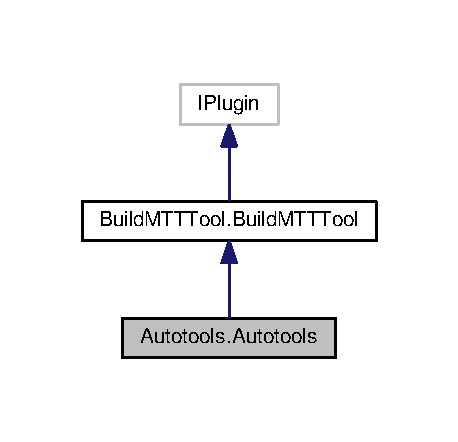
\includegraphics[width=220pt]{class_autotools_1_1_autotools__inherit__graph}
\end{center}
\end{figure}


Collaboration diagram for Autotools.\-Autotools\-:
\nopagebreak
\begin{figure}[H]
\begin{center}
\leavevmode
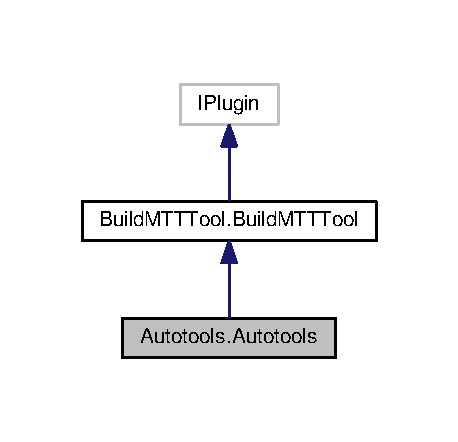
\includegraphics[width=220pt]{class_autotools_1_1_autotools__coll__graph}
\end{center}
\end{figure}
\subsection*{Public Member Functions}
\begin{DoxyCompactItemize}
\item 
def \hyperlink{group___tools_ga5b5ac092ad7f4bc45bf785633c8be95a}{\-\_\-\-\_\-init\-\_\-\-\_\-}
\item 
def \hyperlink{group___tools_ga202b0e727db575d20a381cd039dd3597}{activate}
\item 
def \hyperlink{group___tools_ga74513a2f4135b506e66c047559f9571e}{deactivate}
\item 
def \hyperlink{group___tools_ga0873459245ef2255a5a7386957fa592e}{print\-\_\-name}
\item 
def \hyperlink{group___tools_ga41481e9f2a7e7fce32f51cc8feb909fd}{print\-\_\-options}
\item 
def \hyperlink{group___tools_ga5ae85e70e9e6252f4be23ef60624f633}{execute}
\end{DoxyCompactItemize}
\subsection*{Public Attributes}
\begin{DoxyCompactItemize}
\item 
\hyperlink{group___tools_ga6bbb714a91bc8b6fe749326772b073b3}{activated}
\item 
\hyperlink{group___tools_ga8b348e19f0a7104bde9c43c3a6ed695d}{options}
\item 
\hyperlink{group___tools_gaee37d9789ea22ee310ebc357cd721b7f}{exclude}
\end{DoxyCompactItemize}


\subsection{Detailed Description}


Definition at line 39 of file Autotools.\-py.



The documentation for this class was generated from the following file\-:\begin{DoxyCompactItemize}
\item 
/home/travis/build/open-\/mpi/mtt/pylib/\-Tools/\-Build/\hyperlink{_autotools_8py}{Autotools.\-py}\end{DoxyCompactItemize}

\hypertarget{class_base_m_t_t_utility_1_1_base_m_t_t_utility}{\section{Base\-M\-T\-T\-Utility.\-Base\-M\-T\-T\-Utility Class Reference}
\label{class_base_m_t_t_utility_1_1_base_m_t_t_utility}\index{Base\-M\-T\-T\-Utility.\-Base\-M\-T\-T\-Utility@{Base\-M\-T\-T\-Utility.\-Base\-M\-T\-T\-Utility}}
}


Inheritance diagram for Base\-M\-T\-T\-Utility.\-Base\-M\-T\-T\-Utility\-:
\nopagebreak
\begin{figure}[H]
\begin{center}
\leavevmode
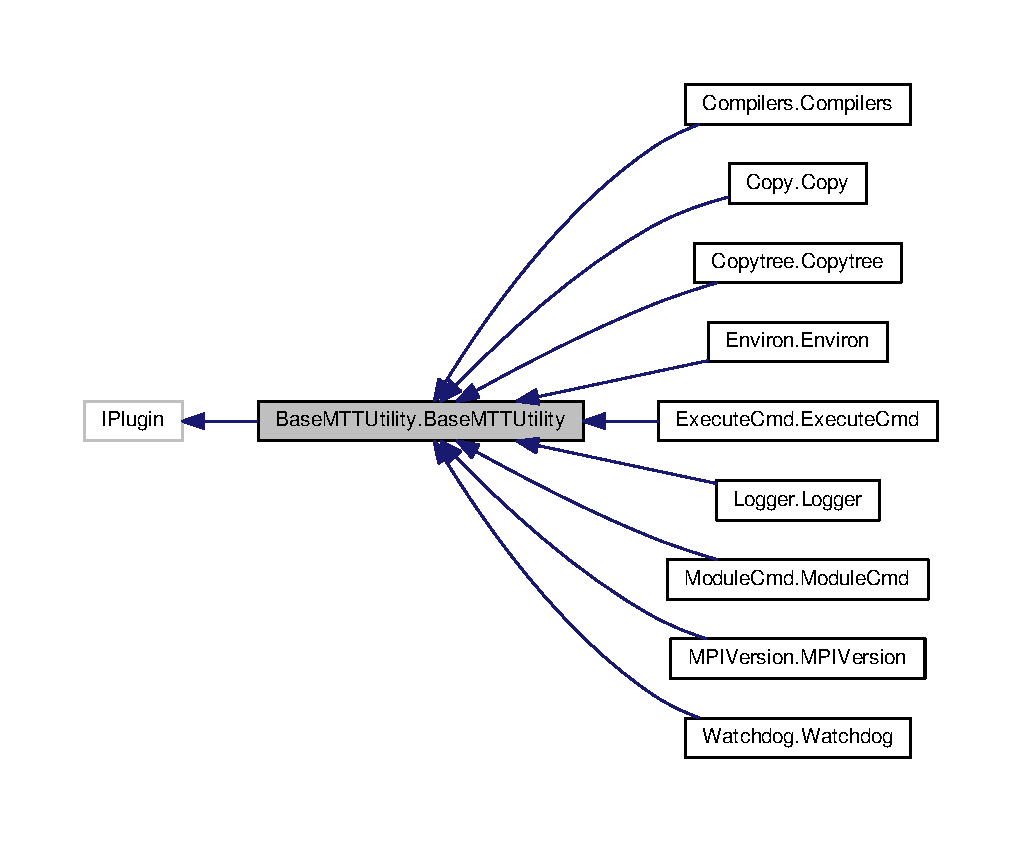
\includegraphics[width=350pt]{class_base_m_t_t_utility_1_1_base_m_t_t_utility__inherit__graph}
\end{center}
\end{figure}


Collaboration diagram for Base\-M\-T\-T\-Utility.\-Base\-M\-T\-T\-Utility\-:
\nopagebreak
\begin{figure}[H]
\begin{center}
\leavevmode
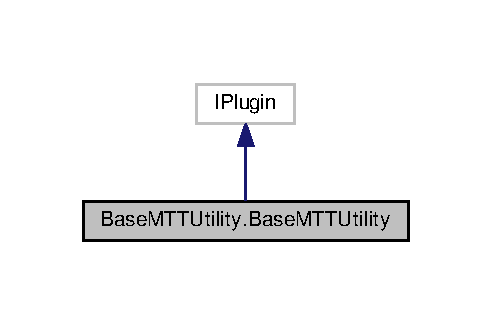
\includegraphics[width=236pt]{class_base_m_t_t_utility_1_1_base_m_t_t_utility__coll__graph}
\end{center}
\end{figure}
\subsection*{Public Member Functions}
\begin{DoxyCompactItemize}
\item 
def \hyperlink{class_base_m_t_t_utility_1_1_base_m_t_t_utility_acc17cee13f814473c5cea32a8e2eebeb}{\-\_\-\-\_\-init\-\_\-\-\_\-}
\item 
def \hyperlink{class_base_m_t_t_utility_1_1_base_m_t_t_utility_a65cd8c577d1fea0bf1edc05969fbe31e}{print\-\_\-name}
\end{DoxyCompactItemize}


\subsection{Detailed Description}


Definition at line 14 of file Base\-M\-T\-T\-Utility.\-py.



\subsection{Constructor \& Destructor Documentation}
\hypertarget{class_base_m_t_t_utility_1_1_base_m_t_t_utility_acc17cee13f814473c5cea32a8e2eebeb}{\index{Base\-M\-T\-T\-Utility\-::\-Base\-M\-T\-T\-Utility@{Base\-M\-T\-T\-Utility\-::\-Base\-M\-T\-T\-Utility}!\-\_\-\-\_\-init\-\_\-\-\_\-@{\-\_\-\-\_\-init\-\_\-\-\_\-}}
\index{\-\_\-\-\_\-init\-\_\-\-\_\-@{\-\_\-\-\_\-init\-\_\-\-\_\-}!BaseMTTUtility::BaseMTTUtility@{Base\-M\-T\-T\-Utility\-::\-Base\-M\-T\-T\-Utility}}
\subsubsection[{\-\_\-\-\_\-init\-\_\-\-\_\-}]{\setlength{\rightskip}{0pt plus 5cm}def Base\-M\-T\-T\-Utility.\-Base\-M\-T\-T\-Utility.\-\_\-\-\_\-init\-\_\-\-\_\- (
\begin{DoxyParamCaption}
\item[{}]{self}
\end{DoxyParamCaption}
)}}\label{class_base_m_t_t_utility_1_1_base_m_t_t_utility_acc17cee13f814473c5cea32a8e2eebeb}


Definition at line 15 of file Base\-M\-T\-T\-Utility.\-py.



\subsection{Member Function Documentation}
\hypertarget{class_base_m_t_t_utility_1_1_base_m_t_t_utility_a65cd8c577d1fea0bf1edc05969fbe31e}{\index{Base\-M\-T\-T\-Utility\-::\-Base\-M\-T\-T\-Utility@{Base\-M\-T\-T\-Utility\-::\-Base\-M\-T\-T\-Utility}!print\-\_\-name@{print\-\_\-name}}
\index{print\-\_\-name@{print\-\_\-name}!BaseMTTUtility::BaseMTTUtility@{Base\-M\-T\-T\-Utility\-::\-Base\-M\-T\-T\-Utility}}
\subsubsection[{print\-\_\-name}]{\setlength{\rightskip}{0pt plus 5cm}def Base\-M\-T\-T\-Utility.\-Base\-M\-T\-T\-Utility.\-print\-\_\-name (
\begin{DoxyParamCaption}
\item[{}]{self}
\end{DoxyParamCaption}
)}}\label{class_base_m_t_t_utility_1_1_base_m_t_t_utility_a65cd8c577d1fea0bf1edc05969fbe31e}


Definition at line 19 of file Base\-M\-T\-T\-Utility.\-py.



The documentation for this class was generated from the following file\-:\begin{DoxyCompactItemize}
\item 
/home/travis/build/open-\/mpi/mtt/pylib/\-Utilities/\hyperlink{_base_m_t_t_utility_8py}{Base\-M\-T\-T\-Utility.\-py}\end{DoxyCompactItemize}

\hypertarget{class_b_i_o_s_m_t_t_stage_1_1_b_i_o_s_m_t_t_stage}{\section{B\-I\-O\-S\-M\-T\-T\-Stage.\-B\-I\-O\-S\-M\-T\-T\-Stage Class Reference}
\label{class_b_i_o_s_m_t_t_stage_1_1_b_i_o_s_m_t_t_stage}\index{B\-I\-O\-S\-M\-T\-T\-Stage.\-B\-I\-O\-S\-M\-T\-T\-Stage@{B\-I\-O\-S\-M\-T\-T\-Stage.\-B\-I\-O\-S\-M\-T\-T\-Stage}}
}


Inheritance diagram for B\-I\-O\-S\-M\-T\-T\-Stage.\-B\-I\-O\-S\-M\-T\-T\-Stage\-:
\nopagebreak
\begin{figure}[H]
\begin{center}
\leavevmode
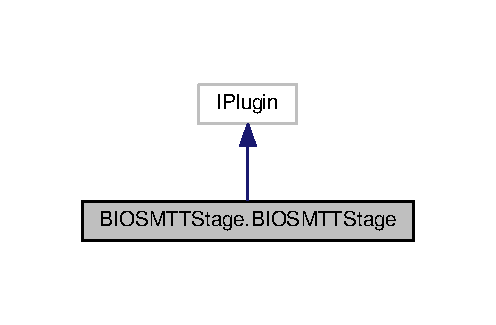
\includegraphics[width=238pt]{class_b_i_o_s_m_t_t_stage_1_1_b_i_o_s_m_t_t_stage__inherit__graph}
\end{center}
\end{figure}


Collaboration diagram for B\-I\-O\-S\-M\-T\-T\-Stage.\-B\-I\-O\-S\-M\-T\-T\-Stage\-:
\nopagebreak
\begin{figure}[H]
\begin{center}
\leavevmode
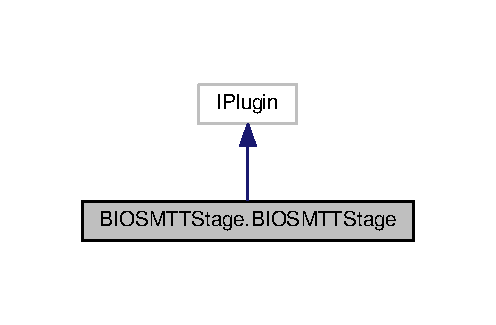
\includegraphics[width=238pt]{class_b_i_o_s_m_t_t_stage_1_1_b_i_o_s_m_t_t_stage__coll__graph}
\end{center}
\end{figure}
\subsection*{Public Member Functions}
\begin{DoxyCompactItemize}
\item 
def \hyperlink{class_b_i_o_s_m_t_t_stage_1_1_b_i_o_s_m_t_t_stage_aa5f27b6db5d3b10cbd5d6e47de378e58}{\-\_\-\-\_\-init\-\_\-\-\_\-}
\item 
def \hyperlink{class_b_i_o_s_m_t_t_stage_1_1_b_i_o_s_m_t_t_stage_a4e5d3ca4920bd6825cdda7259fa85d52}{print\-\_\-name}
\item 
def \hyperlink{class_b_i_o_s_m_t_t_stage_1_1_b_i_o_s_m_t_t_stage_ae46a6ddd03499b39c15d164ea3643e48}{ordering}
\end{DoxyCompactItemize}


\subsection{Detailed Description}


Definition at line 19 of file B\-I\-O\-S\-M\-T\-T\-Stage.\-py.



\subsection{Constructor \& Destructor Documentation}
\hypertarget{class_b_i_o_s_m_t_t_stage_1_1_b_i_o_s_m_t_t_stage_aa5f27b6db5d3b10cbd5d6e47de378e58}{\index{B\-I\-O\-S\-M\-T\-T\-Stage\-::\-B\-I\-O\-S\-M\-T\-T\-Stage@{B\-I\-O\-S\-M\-T\-T\-Stage\-::\-B\-I\-O\-S\-M\-T\-T\-Stage}!\-\_\-\-\_\-init\-\_\-\-\_\-@{\-\_\-\-\_\-init\-\_\-\-\_\-}}
\index{\-\_\-\-\_\-init\-\_\-\-\_\-@{\-\_\-\-\_\-init\-\_\-\-\_\-}!BIOSMTTStage::BIOSMTTStage@{B\-I\-O\-S\-M\-T\-T\-Stage\-::\-B\-I\-O\-S\-M\-T\-T\-Stage}}
\subsubsection[{\-\_\-\-\_\-init\-\_\-\-\_\-}]{\setlength{\rightskip}{0pt plus 5cm}def B\-I\-O\-S\-M\-T\-T\-Stage.\-B\-I\-O\-S\-M\-T\-T\-Stage.\-\_\-\-\_\-init\-\_\-\-\_\- (
\begin{DoxyParamCaption}
\item[{}]{self}
\end{DoxyParamCaption}
)}}\label{class_b_i_o_s_m_t_t_stage_1_1_b_i_o_s_m_t_t_stage_aa5f27b6db5d3b10cbd5d6e47de378e58}


Definition at line 20 of file B\-I\-O\-S\-M\-T\-T\-Stage.\-py.



\subsection{Member Function Documentation}
\hypertarget{class_b_i_o_s_m_t_t_stage_1_1_b_i_o_s_m_t_t_stage_ae46a6ddd03499b39c15d164ea3643e48}{\index{B\-I\-O\-S\-M\-T\-T\-Stage\-::\-B\-I\-O\-S\-M\-T\-T\-Stage@{B\-I\-O\-S\-M\-T\-T\-Stage\-::\-B\-I\-O\-S\-M\-T\-T\-Stage}!ordering@{ordering}}
\index{ordering@{ordering}!BIOSMTTStage::BIOSMTTStage@{B\-I\-O\-S\-M\-T\-T\-Stage\-::\-B\-I\-O\-S\-M\-T\-T\-Stage}}
\subsubsection[{ordering}]{\setlength{\rightskip}{0pt plus 5cm}def B\-I\-O\-S\-M\-T\-T\-Stage.\-B\-I\-O\-S\-M\-T\-T\-Stage.\-ordering (
\begin{DoxyParamCaption}
\item[{}]{self}
\end{DoxyParamCaption}
)}}\label{class_b_i_o_s_m_t_t_stage_1_1_b_i_o_s_m_t_t_stage_ae46a6ddd03499b39c15d164ea3643e48}


Definition at line 26 of file B\-I\-O\-S\-M\-T\-T\-Stage.\-py.

\hypertarget{class_b_i_o_s_m_t_t_stage_1_1_b_i_o_s_m_t_t_stage_a4e5d3ca4920bd6825cdda7259fa85d52}{\index{B\-I\-O\-S\-M\-T\-T\-Stage\-::\-B\-I\-O\-S\-M\-T\-T\-Stage@{B\-I\-O\-S\-M\-T\-T\-Stage\-::\-B\-I\-O\-S\-M\-T\-T\-Stage}!print\-\_\-name@{print\-\_\-name}}
\index{print\-\_\-name@{print\-\_\-name}!BIOSMTTStage::BIOSMTTStage@{B\-I\-O\-S\-M\-T\-T\-Stage\-::\-B\-I\-O\-S\-M\-T\-T\-Stage}}
\subsubsection[{print\-\_\-name}]{\setlength{\rightskip}{0pt plus 5cm}def B\-I\-O\-S\-M\-T\-T\-Stage.\-B\-I\-O\-S\-M\-T\-T\-Stage.\-print\-\_\-name (
\begin{DoxyParamCaption}
\item[{}]{self}
\end{DoxyParamCaption}
)}}\label{class_b_i_o_s_m_t_t_stage_1_1_b_i_o_s_m_t_t_stage_a4e5d3ca4920bd6825cdda7259fa85d52}


Definition at line 23 of file B\-I\-O\-S\-M\-T\-T\-Stage.\-py.



The documentation for this class was generated from the following file\-:\begin{DoxyCompactItemize}
\item 
/home/travis/build/open-\/mpi/mtt/pylib/\-Stages/\-B\-I\-O\-S/\hyperlink{_b_i_o_s_m_t_t_stage_8py}{B\-I\-O\-S\-M\-T\-T\-Stage.\-py}\end{DoxyCompactItemize}

\hypertarget{class_build_m_t_t_tool_1_1_build_m_t_t_tool}{\section{Build\-M\-T\-T\-Tool.\-Build\-M\-T\-T\-Tool Class Reference}
\label{class_build_m_t_t_tool_1_1_build_m_t_t_tool}\index{Build\-M\-T\-T\-Tool.\-Build\-M\-T\-T\-Tool@{Build\-M\-T\-T\-Tool.\-Build\-M\-T\-T\-Tool}}
}


Inheritance diagram for Build\-M\-T\-T\-Tool.\-Build\-M\-T\-T\-Tool\-:
\nopagebreak
\begin{figure}[H]
\begin{center}
\leavevmode
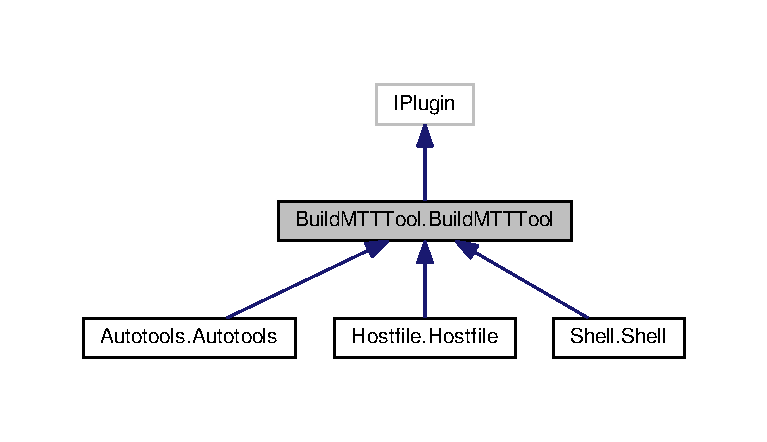
\includegraphics[width=350pt]{class_build_m_t_t_tool_1_1_build_m_t_t_tool__inherit__graph}
\end{center}
\end{figure}


Collaboration diagram for Build\-M\-T\-T\-Tool.\-Build\-M\-T\-T\-Tool\-:
\nopagebreak
\begin{figure}[H]
\begin{center}
\leavevmode
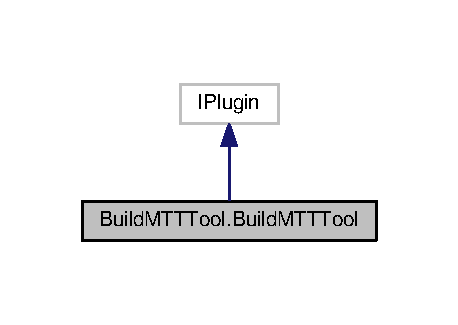
\includegraphics[width=220pt]{class_build_m_t_t_tool_1_1_build_m_t_t_tool__coll__graph}
\end{center}
\end{figure}
\subsection*{Public Member Functions}
\begin{DoxyCompactItemize}
\item 
def \hyperlink{class_build_m_t_t_tool_1_1_build_m_t_t_tool_a5665b0ed7a6ef42181601533cdbe74be}{\-\_\-\-\_\-init\-\_\-\-\_\-}
\item 
def \hyperlink{class_build_m_t_t_tool_1_1_build_m_t_t_tool_afbb7e8957f4c8c43e2937489173de162}{print\-\_\-name}
\end{DoxyCompactItemize}


\subsection{Detailed Description}


Definition at line 19 of file Build\-M\-T\-T\-Tool.\-py.



\subsection{Constructor \& Destructor Documentation}
\hypertarget{class_build_m_t_t_tool_1_1_build_m_t_t_tool_a5665b0ed7a6ef42181601533cdbe74be}{\index{Build\-M\-T\-T\-Tool\-::\-Build\-M\-T\-T\-Tool@{Build\-M\-T\-T\-Tool\-::\-Build\-M\-T\-T\-Tool}!\-\_\-\-\_\-init\-\_\-\-\_\-@{\-\_\-\-\_\-init\-\_\-\-\_\-}}
\index{\-\_\-\-\_\-init\-\_\-\-\_\-@{\-\_\-\-\_\-init\-\_\-\-\_\-}!BuildMTTTool::BuildMTTTool@{Build\-M\-T\-T\-Tool\-::\-Build\-M\-T\-T\-Tool}}
\subsubsection[{\-\_\-\-\_\-init\-\_\-\-\_\-}]{\setlength{\rightskip}{0pt plus 5cm}def Build\-M\-T\-T\-Tool.\-Build\-M\-T\-T\-Tool.\-\_\-\-\_\-init\-\_\-\-\_\- (
\begin{DoxyParamCaption}
\item[{}]{self}
\end{DoxyParamCaption}
)}}\label{class_build_m_t_t_tool_1_1_build_m_t_t_tool_a5665b0ed7a6ef42181601533cdbe74be}


Definition at line 20 of file Build\-M\-T\-T\-Tool.\-py.



\subsection{Member Function Documentation}
\hypertarget{class_build_m_t_t_tool_1_1_build_m_t_t_tool_afbb7e8957f4c8c43e2937489173de162}{\index{Build\-M\-T\-T\-Tool\-::\-Build\-M\-T\-T\-Tool@{Build\-M\-T\-T\-Tool\-::\-Build\-M\-T\-T\-Tool}!print\-\_\-name@{print\-\_\-name}}
\index{print\-\_\-name@{print\-\_\-name}!BuildMTTTool::BuildMTTTool@{Build\-M\-T\-T\-Tool\-::\-Build\-M\-T\-T\-Tool}}
\subsubsection[{print\-\_\-name}]{\setlength{\rightskip}{0pt plus 5cm}def Build\-M\-T\-T\-Tool.\-Build\-M\-T\-T\-Tool.\-print\-\_\-name (
\begin{DoxyParamCaption}
\item[{}]{self}
\end{DoxyParamCaption}
)}}\label{class_build_m_t_t_tool_1_1_build_m_t_t_tool_afbb7e8957f4c8c43e2937489173de162}


Definition at line 24 of file Build\-M\-T\-T\-Tool.\-py.



The documentation for this class was generated from the following file\-:\begin{DoxyCompactItemize}
\item 
/home/travis/build/open-\/mpi/mtt/pylib/\-Tools/\-Build/\hyperlink{_build_m_t_t_tool_8py}{Build\-M\-T\-T\-Tool.\-py}\end{DoxyCompactItemize}

\hypertarget{class_check_profile_1_1_check_profile}{\section{Check\-Profile.\-Check\-Profile Class Reference}
\label{class_check_profile_1_1_check_profile}\index{Check\-Profile.\-Check\-Profile@{Check\-Profile.\-Check\-Profile}}
}


Inheritance diagram for Check\-Profile.\-Check\-Profile\-:
\nopagebreak
\begin{figure}[H]
\begin{center}
\leavevmode
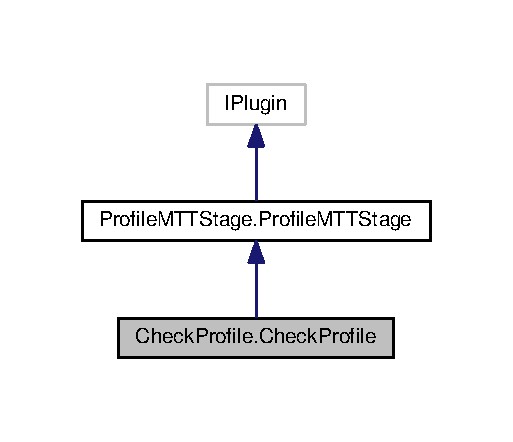
\includegraphics[width=246pt]{class_check_profile_1_1_check_profile__inherit__graph}
\end{center}
\end{figure}


Collaboration diagram for Check\-Profile.\-Check\-Profile\-:
\nopagebreak
\begin{figure}[H]
\begin{center}
\leavevmode
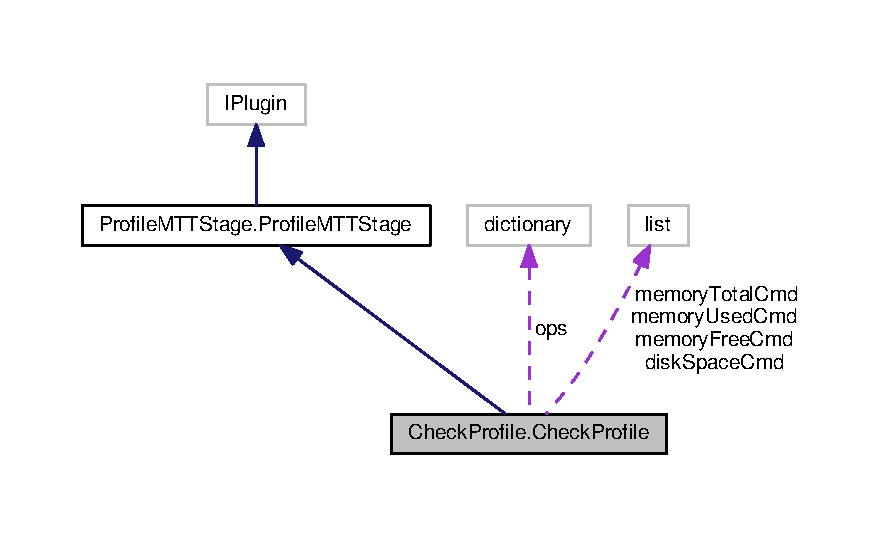
\includegraphics[width=350pt]{class_check_profile_1_1_check_profile__coll__graph}
\end{center}
\end{figure}
\subsection*{Public Member Functions}
\begin{DoxyCompactItemize}
\item 
def \hyperlink{class_check_profile_1_1_check_profile_a59610ed60307ee5ae57651f34bf9529f}{\-\_\-\-\_\-init\-\_\-\-\_\-}
\item 
def \hyperlink{class_check_profile_1_1_check_profile_a24038337f9ee0ed6741e38121fefc8c8}{activate}
\item 
def \hyperlink{class_check_profile_1_1_check_profile_ae499aa8259bdb20f403cb1bf84909939}{deactivate}
\item 
def \hyperlink{class_check_profile_1_1_check_profile_a7b456afd6026cac14021c21c5ad850f3}{print\-\_\-name}
\item 
def \hyperlink{class_check_profile_1_1_check_profile_aee55aa9f7021cb65097a5a485985df7c}{print\-\_\-options}
\item 
def \hyperlink{class_check_profile_1_1_check_profile_ad3ef683b23f6127a7a31373d00a7f1dc}{execute}
\end{DoxyCompactItemize}
\subsection*{Public Attributes}
\begin{DoxyCompactItemize}
\item 
\hyperlink{class_check_profile_1_1_check_profile_a60bdbb946d15fb43c2e465bb8a3fff99}{options}
\end{DoxyCompactItemize}
\subsection*{Static Public Attributes}
\begin{DoxyCompactItemize}
\item 
list \hyperlink{class_check_profile_1_1_check_profile_a074cbe798e2d4fa35fc83aa33a307b6c}{disk\-Space\-Cmd} = \mbox{[}\char`\"{}sh\char`\"{}, \char`\"{}-\/c\char`\"{}, \char`\"{}df -\/B\-M -\/-\/output=pcent D\-I\-S\-K $\vert$ grep -\/v Use\char`\"{}\mbox{]}
\item 
list \hyperlink{class_check_profile_1_1_check_profile_a8a9c2299135872cfccf2b0cb25ba854b}{memory\-Free\-Cmd} = \mbox{[}\char`\"{}sh\char`\"{}, \char`\"{}-\/c\char`\"{}, \char`\"{}free -\/h -\/o $\vert$ grep Mem\-: $\vert$ awk '\{print \$4\}'\char`\"{}\mbox{]}
\item 
list \hyperlink{class_check_profile_1_1_check_profile_a097bc2442305e7d6eebaff44a53c16f3}{memory\-Total\-Cmd} = \mbox{[}\char`\"{}sh\char`\"{}, \char`\"{}-\/c\char`\"{}, \char`\"{}free -\/h -\/o $\vert$ grep Mem\-: $\vert$ awk '\{print \$2\}'\char`\"{}\mbox{]}
\item 
list \hyperlink{class_check_profile_1_1_check_profile_a3c36cf35599b47c7158008533cc9cb39}{memory\-Used\-Cmd} = \mbox{[}\char`\"{}sh\char`\"{}, \char`\"{}-\/c\char`\"{}, \char`\"{}free -\/h -\/o $\vert$ grep Mem\-: $\vert$ awk '\{print \$3\}'\char`\"{}\mbox{]}
\item 
dictionary \hyperlink{class_check_profile_1_1_check_profile_aa4e92c1c6def969cc4a347111d4ef0de}{ops}
\end{DoxyCompactItemize}


\subsection{Detailed Description}


Definition at line 25 of file Check\-Profile.\-py.



\subsection{Constructor \& Destructor Documentation}
\hypertarget{class_check_profile_1_1_check_profile_a59610ed60307ee5ae57651f34bf9529f}{\index{Check\-Profile\-::\-Check\-Profile@{Check\-Profile\-::\-Check\-Profile}!\-\_\-\-\_\-init\-\_\-\-\_\-@{\-\_\-\-\_\-init\-\_\-\-\_\-}}
\index{\-\_\-\-\_\-init\-\_\-\-\_\-@{\-\_\-\-\_\-init\-\_\-\-\_\-}!CheckProfile::CheckProfile@{Check\-Profile\-::\-Check\-Profile}}
\subsubsection[{\-\_\-\-\_\-init\-\_\-\-\_\-}]{\setlength{\rightskip}{0pt plus 5cm}def Check\-Profile.\-Check\-Profile.\-\_\-\-\_\-init\-\_\-\-\_\- (
\begin{DoxyParamCaption}
\item[{}]{self}
\end{DoxyParamCaption}
)}}\label{class_check_profile_1_1_check_profile_a59610ed60307ee5ae57651f34bf9529f}


Definition at line 39 of file Check\-Profile.\-py.



\subsection{Member Function Documentation}
\hypertarget{class_check_profile_1_1_check_profile_a24038337f9ee0ed6741e38121fefc8c8}{\index{Check\-Profile\-::\-Check\-Profile@{Check\-Profile\-::\-Check\-Profile}!activate@{activate}}
\index{activate@{activate}!CheckProfile::CheckProfile@{Check\-Profile\-::\-Check\-Profile}}
\subsubsection[{activate}]{\setlength{\rightskip}{0pt plus 5cm}def Check\-Profile.\-Check\-Profile.\-activate (
\begin{DoxyParamCaption}
\item[{}]{self}
\end{DoxyParamCaption}
)}}\label{class_check_profile_1_1_check_profile_a24038337f9ee0ed6741e38121fefc8c8}


Definition at line 50 of file Check\-Profile.\-py.

\hypertarget{class_check_profile_1_1_check_profile_ae499aa8259bdb20f403cb1bf84909939}{\index{Check\-Profile\-::\-Check\-Profile@{Check\-Profile\-::\-Check\-Profile}!deactivate@{deactivate}}
\index{deactivate@{deactivate}!CheckProfile::CheckProfile@{Check\-Profile\-::\-Check\-Profile}}
\subsubsection[{deactivate}]{\setlength{\rightskip}{0pt plus 5cm}def Check\-Profile.\-Check\-Profile.\-deactivate (
\begin{DoxyParamCaption}
\item[{}]{self}
\end{DoxyParamCaption}
)}}\label{class_check_profile_1_1_check_profile_ae499aa8259bdb20f403cb1bf84909939}


Definition at line 56 of file Check\-Profile.\-py.

\hypertarget{class_check_profile_1_1_check_profile_ad3ef683b23f6127a7a31373d00a7f1dc}{\index{Check\-Profile\-::\-Check\-Profile@{Check\-Profile\-::\-Check\-Profile}!execute@{execute}}
\index{execute@{execute}!CheckProfile::CheckProfile@{Check\-Profile\-::\-Check\-Profile}}
\subsubsection[{execute}]{\setlength{\rightskip}{0pt plus 5cm}def Check\-Profile.\-Check\-Profile.\-execute (
\begin{DoxyParamCaption}
\item[{}]{self, }
\item[{}]{log, }
\item[{}]{keyvals, }
\item[{}]{test\-Def}
\end{DoxyParamCaption}
)}}\label{class_check_profile_1_1_check_profile_ad3ef683b23f6127a7a31373d00a7f1dc}


Definition at line 69 of file Check\-Profile.\-py.

\hypertarget{class_check_profile_1_1_check_profile_a7b456afd6026cac14021c21c5ad850f3}{\index{Check\-Profile\-::\-Check\-Profile@{Check\-Profile\-::\-Check\-Profile}!print\-\_\-name@{print\-\_\-name}}
\index{print\-\_\-name@{print\-\_\-name}!CheckProfile::CheckProfile@{Check\-Profile\-::\-Check\-Profile}}
\subsubsection[{print\-\_\-name}]{\setlength{\rightskip}{0pt plus 5cm}def Check\-Profile.\-Check\-Profile.\-print\-\_\-name (
\begin{DoxyParamCaption}
\item[{}]{self}
\end{DoxyParamCaption}
)}}\label{class_check_profile_1_1_check_profile_a7b456afd6026cac14021c21c5ad850f3}


Definition at line 60 of file Check\-Profile.\-py.

\hypertarget{class_check_profile_1_1_check_profile_aee55aa9f7021cb65097a5a485985df7c}{\index{Check\-Profile\-::\-Check\-Profile@{Check\-Profile\-::\-Check\-Profile}!print\-\_\-options@{print\-\_\-options}}
\index{print\-\_\-options@{print\-\_\-options}!CheckProfile::CheckProfile@{Check\-Profile\-::\-Check\-Profile}}
\subsubsection[{print\-\_\-options}]{\setlength{\rightskip}{0pt plus 5cm}def Check\-Profile.\-Check\-Profile.\-print\-\_\-options (
\begin{DoxyParamCaption}
\item[{}]{self, }
\item[{}]{test\-Def, }
\item[{}]{prefix}
\end{DoxyParamCaption}
)}}\label{class_check_profile_1_1_check_profile_aee55aa9f7021cb65097a5a485985df7c}


Definition at line 63 of file Check\-Profile.\-py.



\subsection{Member Data Documentation}
\hypertarget{class_check_profile_1_1_check_profile_a074cbe798e2d4fa35fc83aa33a307b6c}{\index{Check\-Profile\-::\-Check\-Profile@{Check\-Profile\-::\-Check\-Profile}!disk\-Space\-Cmd@{disk\-Space\-Cmd}}
\index{disk\-Space\-Cmd@{disk\-Space\-Cmd}!CheckProfile::CheckProfile@{Check\-Profile\-::\-Check\-Profile}}
\subsubsection[{disk\-Space\-Cmd}]{\setlength{\rightskip}{0pt plus 5cm}list Check\-Profile.\-Check\-Profile.\-disk\-Space\-Cmd = \mbox{[}\char`\"{}sh\char`\"{}, \char`\"{}-\/c\char`\"{}, \char`\"{}df -\/B\-M -\/-\/output=pcent D\-I\-S\-K $\vert$ grep -\/v Use\char`\"{}\mbox{]}\hspace{0.3cm}{\ttfamily [static]}}}\label{class_check_profile_1_1_check_profile_a074cbe798e2d4fa35fc83aa33a307b6c}


Definition at line 27 of file Check\-Profile.\-py.

\hypertarget{class_check_profile_1_1_check_profile_a8a9c2299135872cfccf2b0cb25ba854b}{\index{Check\-Profile\-::\-Check\-Profile@{Check\-Profile\-::\-Check\-Profile}!memory\-Free\-Cmd@{memory\-Free\-Cmd}}
\index{memory\-Free\-Cmd@{memory\-Free\-Cmd}!CheckProfile::CheckProfile@{Check\-Profile\-::\-Check\-Profile}}
\subsubsection[{memory\-Free\-Cmd}]{\setlength{\rightskip}{0pt plus 5cm}list Check\-Profile.\-Check\-Profile.\-memory\-Free\-Cmd = \mbox{[}\char`\"{}sh\char`\"{}, \char`\"{}-\/c\char`\"{}, \char`\"{}free -\/h -\/o $\vert$ grep Mem\-: $\vert$ awk '\{print \$4\}'\char`\"{}\mbox{]}\hspace{0.3cm}{\ttfamily [static]}}}\label{class_check_profile_1_1_check_profile_a8a9c2299135872cfccf2b0cb25ba854b}


Definition at line 28 of file Check\-Profile.\-py.

\hypertarget{class_check_profile_1_1_check_profile_a097bc2442305e7d6eebaff44a53c16f3}{\index{Check\-Profile\-::\-Check\-Profile@{Check\-Profile\-::\-Check\-Profile}!memory\-Total\-Cmd@{memory\-Total\-Cmd}}
\index{memory\-Total\-Cmd@{memory\-Total\-Cmd}!CheckProfile::CheckProfile@{Check\-Profile\-::\-Check\-Profile}}
\subsubsection[{memory\-Total\-Cmd}]{\setlength{\rightskip}{0pt plus 5cm}list Check\-Profile.\-Check\-Profile.\-memory\-Total\-Cmd = \mbox{[}\char`\"{}sh\char`\"{}, \char`\"{}-\/c\char`\"{}, \char`\"{}free -\/h -\/o $\vert$ grep Mem\-: $\vert$ awk '\{print \$2\}'\char`\"{}\mbox{]}\hspace{0.3cm}{\ttfamily [static]}}}\label{class_check_profile_1_1_check_profile_a097bc2442305e7d6eebaff44a53c16f3}


Definition at line 29 of file Check\-Profile.\-py.

\hypertarget{class_check_profile_1_1_check_profile_a3c36cf35599b47c7158008533cc9cb39}{\index{Check\-Profile\-::\-Check\-Profile@{Check\-Profile\-::\-Check\-Profile}!memory\-Used\-Cmd@{memory\-Used\-Cmd}}
\index{memory\-Used\-Cmd@{memory\-Used\-Cmd}!CheckProfile::CheckProfile@{Check\-Profile\-::\-Check\-Profile}}
\subsubsection[{memory\-Used\-Cmd}]{\setlength{\rightskip}{0pt plus 5cm}list Check\-Profile.\-Check\-Profile.\-memory\-Used\-Cmd = \mbox{[}\char`\"{}sh\char`\"{}, \char`\"{}-\/c\char`\"{}, \char`\"{}free -\/h -\/o $\vert$ grep Mem\-: $\vert$ awk '\{print \$3\}'\char`\"{}\mbox{]}\hspace{0.3cm}{\ttfamily [static]}}}\label{class_check_profile_1_1_check_profile_a3c36cf35599b47c7158008533cc9cb39}


Definition at line 30 of file Check\-Profile.\-py.

\hypertarget{class_check_profile_1_1_check_profile_aa4e92c1c6def969cc4a347111d4ef0de}{\index{Check\-Profile\-::\-Check\-Profile@{Check\-Profile\-::\-Check\-Profile}!ops@{ops}}
\index{ops@{ops}!CheckProfile::CheckProfile@{Check\-Profile\-::\-Check\-Profile}}
\subsubsection[{ops}]{\setlength{\rightskip}{0pt plus 5cm}dictionary Check\-Profile.\-Check\-Profile.\-ops\hspace{0.3cm}{\ttfamily [static]}}}\label{class_check_profile_1_1_check_profile_aa4e92c1c6def969cc4a347111d4ef0de}
{\bfseries Initial value\-:}
\begin{DoxyCode}
1 = \{ \textcolor{stringliteral}{'>'}: operator.gt,
2             \textcolor{stringliteral}{'<'}: operator.lt,
3             \textcolor{stringliteral}{'>='}: operator.ge,
4             \textcolor{stringliteral}{'<='}: operator.le,
5             \textcolor{stringliteral}{'='}: operator.eq
6     \}
\end{DoxyCode}


Definition at line 32 of file Check\-Profile.\-py.

\hypertarget{class_check_profile_1_1_check_profile_a60bdbb946d15fb43c2e465bb8a3fff99}{\index{Check\-Profile\-::\-Check\-Profile@{Check\-Profile\-::\-Check\-Profile}!options@{options}}
\index{options@{options}!CheckProfile::CheckProfile@{Check\-Profile\-::\-Check\-Profile}}
\subsubsection[{options}]{\setlength{\rightskip}{0pt plus 5cm}Check\-Profile.\-Check\-Profile.\-options}}\label{class_check_profile_1_1_check_profile_a60bdbb946d15fb43c2e465bb8a3fff99}


Definition at line 42 of file Check\-Profile.\-py.



The documentation for this class was generated from the following file\-:\begin{DoxyCompactItemize}
\item 
/home/travis/build/open-\/mpi/mtt/pylib/\-Stages/\-Profile/\hyperlink{_check_profile_8py}{Check\-Profile.\-py}\end{DoxyCompactItemize}

\hypertarget{class_c_n_c_m_t_t_tool_1_1_c_n_c_m_t_t_tool}{\section{C\-N\-C\-M\-T\-T\-Tool.\-C\-N\-C\-M\-T\-T\-Tool Class Reference}
\label{class_c_n_c_m_t_t_tool_1_1_c_n_c_m_t_t_tool}\index{C\-N\-C\-M\-T\-T\-Tool.\-C\-N\-C\-M\-T\-T\-Tool@{C\-N\-C\-M\-T\-T\-Tool.\-C\-N\-C\-M\-T\-T\-Tool}}
}


Inheritance diagram for C\-N\-C\-M\-T\-T\-Tool.\-C\-N\-C\-M\-T\-T\-Tool\-:
\nopagebreak
\begin{figure}[H]
\begin{center}
\leavevmode
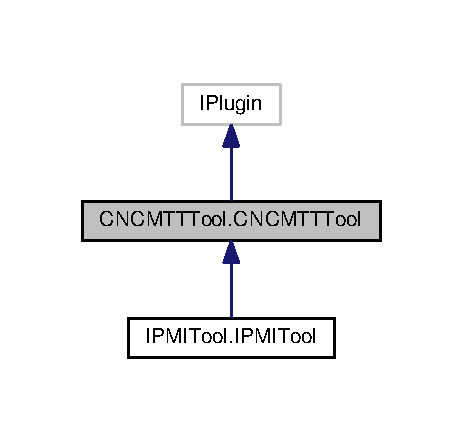
\includegraphics[width=222pt]{class_c_n_c_m_t_t_tool_1_1_c_n_c_m_t_t_tool__inherit__graph}
\end{center}
\end{figure}


Collaboration diagram for C\-N\-C\-M\-T\-T\-Tool.\-C\-N\-C\-M\-T\-T\-Tool\-:
\nopagebreak
\begin{figure}[H]
\begin{center}
\leavevmode
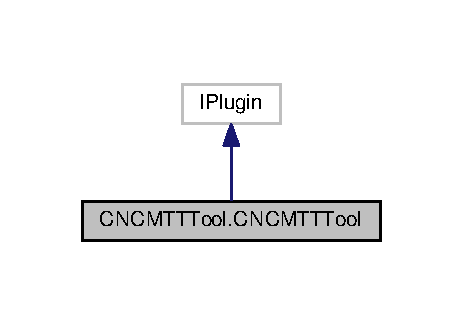
\includegraphics[width=222pt]{class_c_n_c_m_t_t_tool_1_1_c_n_c_m_t_t_tool__coll__graph}
\end{center}
\end{figure}
\subsection*{Public Member Functions}
\begin{DoxyCompactItemize}
\item 
def \hyperlink{class_c_n_c_m_t_t_tool_1_1_c_n_c_m_t_t_tool_a9f2d86b7cd592cae84be27e90d65f862}{\-\_\-\-\_\-init\-\_\-\-\_\-}
\item 
def \hyperlink{class_c_n_c_m_t_t_tool_1_1_c_n_c_m_t_t_tool_a664d4cdf650553342d45bf04981a8e2d}{print\-\_\-name}
\end{DoxyCompactItemize}


\subsection{Detailed Description}


Definition at line 19 of file C\-N\-C\-M\-T\-T\-Tool.\-py.



\subsection{Constructor \& Destructor Documentation}
\hypertarget{class_c_n_c_m_t_t_tool_1_1_c_n_c_m_t_t_tool_a9f2d86b7cd592cae84be27e90d65f862}{\index{C\-N\-C\-M\-T\-T\-Tool\-::\-C\-N\-C\-M\-T\-T\-Tool@{C\-N\-C\-M\-T\-T\-Tool\-::\-C\-N\-C\-M\-T\-T\-Tool}!\-\_\-\-\_\-init\-\_\-\-\_\-@{\-\_\-\-\_\-init\-\_\-\-\_\-}}
\index{\-\_\-\-\_\-init\-\_\-\-\_\-@{\-\_\-\-\_\-init\-\_\-\-\_\-}!CNCMTTTool::CNCMTTTool@{C\-N\-C\-M\-T\-T\-Tool\-::\-C\-N\-C\-M\-T\-T\-Tool}}
\subsubsection[{\-\_\-\-\_\-init\-\_\-\-\_\-}]{\setlength{\rightskip}{0pt plus 5cm}def C\-N\-C\-M\-T\-T\-Tool.\-C\-N\-C\-M\-T\-T\-Tool.\-\_\-\-\_\-init\-\_\-\-\_\- (
\begin{DoxyParamCaption}
\item[{}]{self}
\end{DoxyParamCaption}
)}}\label{class_c_n_c_m_t_t_tool_1_1_c_n_c_m_t_t_tool_a9f2d86b7cd592cae84be27e90d65f862}


Definition at line 20 of file C\-N\-C\-M\-T\-T\-Tool.\-py.



\subsection{Member Function Documentation}
\hypertarget{class_c_n_c_m_t_t_tool_1_1_c_n_c_m_t_t_tool_a664d4cdf650553342d45bf04981a8e2d}{\index{C\-N\-C\-M\-T\-T\-Tool\-::\-C\-N\-C\-M\-T\-T\-Tool@{C\-N\-C\-M\-T\-T\-Tool\-::\-C\-N\-C\-M\-T\-T\-Tool}!print\-\_\-name@{print\-\_\-name}}
\index{print\-\_\-name@{print\-\_\-name}!CNCMTTTool::CNCMTTTool@{C\-N\-C\-M\-T\-T\-Tool\-::\-C\-N\-C\-M\-T\-T\-Tool}}
\subsubsection[{print\-\_\-name}]{\setlength{\rightskip}{0pt plus 5cm}def C\-N\-C\-M\-T\-T\-Tool.\-C\-N\-C\-M\-T\-T\-Tool.\-print\-\_\-name (
\begin{DoxyParamCaption}
\item[{}]{self}
\end{DoxyParamCaption}
)}}\label{class_c_n_c_m_t_t_tool_1_1_c_n_c_m_t_t_tool_a664d4cdf650553342d45bf04981a8e2d}


Definition at line 24 of file C\-N\-C\-M\-T\-T\-Tool.\-py.



The documentation for this class was generated from the following file\-:\begin{DoxyCompactItemize}
\item 
/home/travis/build/open-\/mpi/mtt/pylib/\-Tools/\-C\-N\-C/\hyperlink{_c_n_c_m_t_t_tool_8py}{C\-N\-C\-M\-T\-T\-Tool.\-py}\end{DoxyCompactItemize}

\hypertarget{classcombinatorial_1_1_combinatorial_ex}{\section{combinatorial.\-Combinatorial\-Ex Class Reference}
\label{classcombinatorial_1_1_combinatorial_ex}\index{combinatorial.\-Combinatorial\-Ex@{combinatorial.\-Combinatorial\-Ex}}
}


Inheritance diagram for combinatorial.\-Combinatorial\-Ex\-:
\nopagebreak
\begin{figure}[H]
\begin{center}
\leavevmode
\includegraphics[width=228pt]{classcombinatorial_1_1_combinatorial_ex__inherit__graph}
\end{center}
\end{figure}


Collaboration diagram for combinatorial.\-Combinatorial\-Ex\-:
\nopagebreak
\begin{figure}[H]
\begin{center}
\leavevmode
\includegraphics[width=228pt]{classcombinatorial_1_1_combinatorial_ex__coll__graph}
\end{center}
\end{figure}
\subsection*{Public Member Functions}
\begin{DoxyCompactItemize}
\item 
def \hyperlink{classcombinatorial_1_1_combinatorial_ex_a9a4fbfcf64b1204c14509d348dd23b5d}{\-\_\-\-\_\-init\-\_\-\-\_\-}
\item 
def \hyperlink{classcombinatorial_1_1_combinatorial_ex_a8d0b7c0da355183d8124871bee76b0bd}{activate}
\item 
def \hyperlink{classcombinatorial_1_1_combinatorial_ex_ad53efcff93773cce7ed9cfc2fef38ab3}{deactivate}
\item 
def \hyperlink{classcombinatorial_1_1_combinatorial_ex_a19f6321bf42ab92280c5e3b0a3af89d0}{print\-\_\-name}
\item 
def \hyperlink{classcombinatorial_1_1_combinatorial_ex_ae802ad33a050ada42292e7c80fb3e486}{print\-\_\-options}
\item 
def \hyperlink{classcombinatorial_1_1_combinatorial_ex_ac0216f0d0041c35a91e01ac9dafd49da}{create\-Ini\-Log}
\item 
def \hyperlink{classcombinatorial_1_1_combinatorial_ex_a5a5fbd1692c100374ee458e4babc9832}{execute}
\end{DoxyCompactItemize}
\subsection*{Public Attributes}
\begin{DoxyCompactItemize}
\item 
\hyperlink{classcombinatorial_1_1_combinatorial_ex_a20eda525b3947495bb6084c560dcca27}{options}
\item 
\hyperlink{classcombinatorial_1_1_combinatorial_ex_ab5c27fece8991a34f47e85870637fc91}{parser}
\item 
\hyperlink{classcombinatorial_1_1_combinatorial_ex_a24b3bc621a8380e406bade192bc371d4}{temp\-Dir}
\item 
\hyperlink{classcombinatorial_1_1_combinatorial_ex_a68e6ac6cba4ab4161dd854323e549afd}{base\-Ini\-File}
\item 
\hyperlink{classcombinatorial_1_1_combinatorial_ex_a3de3f7da4c201525da8452258df0bc7b}{run\-Log}
\item 
\hyperlink{classcombinatorial_1_1_combinatorial_ex_a961a46d05fda7be52ea74a5f69df57e2}{ini\-Log}
\end{DoxyCompactItemize}


\subsection{Detailed Description}


Definition at line 33 of file combinatorial.\-py.



\subsection{Constructor \& Destructor Documentation}
\hypertarget{classcombinatorial_1_1_combinatorial_ex_a9a4fbfcf64b1204c14509d348dd23b5d}{\index{combinatorial\-::\-Combinatorial\-Ex@{combinatorial\-::\-Combinatorial\-Ex}!\-\_\-\-\_\-init\-\_\-\-\_\-@{\-\_\-\-\_\-init\-\_\-\-\_\-}}
\index{\-\_\-\-\_\-init\-\_\-\-\_\-@{\-\_\-\-\_\-init\-\_\-\-\_\-}!combinatorial::CombinatorialEx@{combinatorial\-::\-Combinatorial\-Ex}}
\subsubsection[{\-\_\-\-\_\-init\-\_\-\-\_\-}]{\setlength{\rightskip}{0pt plus 5cm}def combinatorial.\-Combinatorial\-Ex.\-\_\-\-\_\-init\-\_\-\-\_\- (
\begin{DoxyParamCaption}
\item[{}]{self}
\end{DoxyParamCaption}
)}}\label{classcombinatorial_1_1_combinatorial_ex_a9a4fbfcf64b1204c14509d348dd23b5d}


Definition at line 35 of file combinatorial.\-py.



\subsection{Member Function Documentation}
\hypertarget{classcombinatorial_1_1_combinatorial_ex_a8d0b7c0da355183d8124871bee76b0bd}{\index{combinatorial\-::\-Combinatorial\-Ex@{combinatorial\-::\-Combinatorial\-Ex}!activate@{activate}}
\index{activate@{activate}!combinatorial::CombinatorialEx@{combinatorial\-::\-Combinatorial\-Ex}}
\subsubsection[{activate}]{\setlength{\rightskip}{0pt plus 5cm}def combinatorial.\-Combinatorial\-Ex.\-activate (
\begin{DoxyParamCaption}
\item[{}]{self}
\end{DoxyParamCaption}
)}}\label{classcombinatorial_1_1_combinatorial_ex_a8d0b7c0da355183d8124871bee76b0bd}


Definition at line 47 of file combinatorial.\-py.

\hypertarget{classcombinatorial_1_1_combinatorial_ex_ac0216f0d0041c35a91e01ac9dafd49da}{\index{combinatorial\-::\-Combinatorial\-Ex@{combinatorial\-::\-Combinatorial\-Ex}!create\-Ini\-Log@{create\-Ini\-Log}}
\index{create\-Ini\-Log@{create\-Ini\-Log}!combinatorial::CombinatorialEx@{combinatorial\-::\-Combinatorial\-Ex}}
\subsubsection[{create\-Ini\-Log}]{\setlength{\rightskip}{0pt plus 5cm}def combinatorial.\-Combinatorial\-Ex.\-create\-Ini\-Log (
\begin{DoxyParamCaption}
\item[{}]{self, }
\item[{}]{test\-Def}
\end{DoxyParamCaption}
)}}\label{classcombinatorial_1_1_combinatorial_ex_ac0216f0d0041c35a91e01ac9dafd49da}


Definition at line 68 of file combinatorial.\-py.



Here is the caller graph for this function\-:
\nopagebreak
\begin{figure}[H]
\begin{center}
\leavevmode
\includegraphics[width=350pt]{classcombinatorial_1_1_combinatorial_ex_ac0216f0d0041c35a91e01ac9dafd49da_icgraph}
\end{center}
\end{figure}


\hypertarget{classcombinatorial_1_1_combinatorial_ex_ad53efcff93773cce7ed9cfc2fef38ab3}{\index{combinatorial\-::\-Combinatorial\-Ex@{combinatorial\-::\-Combinatorial\-Ex}!deactivate@{deactivate}}
\index{deactivate@{deactivate}!combinatorial::CombinatorialEx@{combinatorial\-::\-Combinatorial\-Ex}}
\subsubsection[{deactivate}]{\setlength{\rightskip}{0pt plus 5cm}def combinatorial.\-Combinatorial\-Ex.\-deactivate (
\begin{DoxyParamCaption}
\item[{}]{self}
\end{DoxyParamCaption}
)}}\label{classcombinatorial_1_1_combinatorial_ex_ad53efcff93773cce7ed9cfc2fef38ab3}


Definition at line 52 of file combinatorial.\-py.

\hypertarget{classcombinatorial_1_1_combinatorial_ex_a5a5fbd1692c100374ee458e4babc9832}{\index{combinatorial\-::\-Combinatorial\-Ex@{combinatorial\-::\-Combinatorial\-Ex}!execute@{execute}}
\index{execute@{execute}!combinatorial::CombinatorialEx@{combinatorial\-::\-Combinatorial\-Ex}}
\subsubsection[{execute}]{\setlength{\rightskip}{0pt plus 5cm}def combinatorial.\-Combinatorial\-Ex.\-execute (
\begin{DoxyParamCaption}
\item[{}]{self, }
\item[{}]{test\-Def}
\end{DoxyParamCaption}
)}}\label{classcombinatorial_1_1_combinatorial_ex_a5a5fbd1692c100374ee458e4babc9832}


Definition at line 171 of file combinatorial.\-py.



Here is the call graph for this function\-:
\nopagebreak
\begin{figure}[H]
\begin{center}
\leavevmode
\includegraphics[width=350pt]{classcombinatorial_1_1_combinatorial_ex_a5a5fbd1692c100374ee458e4babc9832_cgraph}
\end{center}
\end{figure}


\hypertarget{classcombinatorial_1_1_combinatorial_ex_a19f6321bf42ab92280c5e3b0a3af89d0}{\index{combinatorial\-::\-Combinatorial\-Ex@{combinatorial\-::\-Combinatorial\-Ex}!print\-\_\-name@{print\-\_\-name}}
\index{print\-\_\-name@{print\-\_\-name}!combinatorial::CombinatorialEx@{combinatorial\-::\-Combinatorial\-Ex}}
\subsubsection[{print\-\_\-name}]{\setlength{\rightskip}{0pt plus 5cm}def combinatorial.\-Combinatorial\-Ex.\-print\-\_\-name (
\begin{DoxyParamCaption}
\item[{}]{self}
\end{DoxyParamCaption}
)}}\label{classcombinatorial_1_1_combinatorial_ex_a19f6321bf42ab92280c5e3b0a3af89d0}


Definition at line 56 of file combinatorial.\-py.

\hypertarget{classcombinatorial_1_1_combinatorial_ex_ae802ad33a050ada42292e7c80fb3e486}{\index{combinatorial\-::\-Combinatorial\-Ex@{combinatorial\-::\-Combinatorial\-Ex}!print\-\_\-options@{print\-\_\-options}}
\index{print\-\_\-options@{print\-\_\-options}!combinatorial::CombinatorialEx@{combinatorial\-::\-Combinatorial\-Ex}}
\subsubsection[{print\-\_\-options}]{\setlength{\rightskip}{0pt plus 5cm}def combinatorial.\-Combinatorial\-Ex.\-print\-\_\-options (
\begin{DoxyParamCaption}
\item[{}]{self, }
\item[{}]{test\-Def, }
\item[{}]{prefix}
\end{DoxyParamCaption}
)}}\label{classcombinatorial_1_1_combinatorial_ex_ae802ad33a050ada42292e7c80fb3e486}


Definition at line 59 of file combinatorial.\-py.



\subsection{Member Data Documentation}
\hypertarget{classcombinatorial_1_1_combinatorial_ex_a68e6ac6cba4ab4161dd854323e549afd}{\index{combinatorial\-::\-Combinatorial\-Ex@{combinatorial\-::\-Combinatorial\-Ex}!base\-Ini\-File@{base\-Ini\-File}}
\index{base\-Ini\-File@{base\-Ini\-File}!combinatorial::CombinatorialEx@{combinatorial\-::\-Combinatorial\-Ex}}
\subsubsection[{base\-Ini\-File}]{\setlength{\rightskip}{0pt plus 5cm}combinatorial.\-Combinatorial\-Ex.\-base\-Ini\-File}}\label{classcombinatorial_1_1_combinatorial_ex_a68e6ac6cba4ab4161dd854323e549afd}


Definition at line 43 of file combinatorial.\-py.

\hypertarget{classcombinatorial_1_1_combinatorial_ex_a961a46d05fda7be52ea74a5f69df57e2}{\index{combinatorial\-::\-Combinatorial\-Ex@{combinatorial\-::\-Combinatorial\-Ex}!ini\-Log@{ini\-Log}}
\index{ini\-Log@{ini\-Log}!combinatorial::CombinatorialEx@{combinatorial\-::\-Combinatorial\-Ex}}
\subsubsection[{ini\-Log}]{\setlength{\rightskip}{0pt plus 5cm}combinatorial.\-Combinatorial\-Ex.\-ini\-Log}}\label{classcombinatorial_1_1_combinatorial_ex_a961a46d05fda7be52ea74a5f69df57e2}


Definition at line 45 of file combinatorial.\-py.

\hypertarget{classcombinatorial_1_1_combinatorial_ex_a20eda525b3947495bb6084c560dcca27}{\index{combinatorial\-::\-Combinatorial\-Ex@{combinatorial\-::\-Combinatorial\-Ex}!options@{options}}
\index{options@{options}!combinatorial::CombinatorialEx@{combinatorial\-::\-Combinatorial\-Ex}}
\subsubsection[{options}]{\setlength{\rightskip}{0pt plus 5cm}combinatorial.\-Combinatorial\-Ex.\-options}}\label{classcombinatorial_1_1_combinatorial_ex_a20eda525b3947495bb6084c560dcca27}


Definition at line 38 of file combinatorial.\-py.

\hypertarget{classcombinatorial_1_1_combinatorial_ex_ab5c27fece8991a34f47e85870637fc91}{\index{combinatorial\-::\-Combinatorial\-Ex@{combinatorial\-::\-Combinatorial\-Ex}!parser@{parser}}
\index{parser@{parser}!combinatorial::CombinatorialEx@{combinatorial\-::\-Combinatorial\-Ex}}
\subsubsection[{parser}]{\setlength{\rightskip}{0pt plus 5cm}combinatorial.\-Combinatorial\-Ex.\-parser}}\label{classcombinatorial_1_1_combinatorial_ex_ab5c27fece8991a34f47e85870637fc91}


Definition at line 39 of file combinatorial.\-py.

\hypertarget{classcombinatorial_1_1_combinatorial_ex_a3de3f7da4c201525da8452258df0bc7b}{\index{combinatorial\-::\-Combinatorial\-Ex@{combinatorial\-::\-Combinatorial\-Ex}!run\-Log@{run\-Log}}
\index{run\-Log@{run\-Log}!combinatorial::CombinatorialEx@{combinatorial\-::\-Combinatorial\-Ex}}
\subsubsection[{run\-Log}]{\setlength{\rightskip}{0pt plus 5cm}combinatorial.\-Combinatorial\-Ex.\-run\-Log}}\label{classcombinatorial_1_1_combinatorial_ex_a3de3f7da4c201525da8452258df0bc7b}


Definition at line 44 of file combinatorial.\-py.

\hypertarget{classcombinatorial_1_1_combinatorial_ex_a24b3bc621a8380e406bade192bc371d4}{\index{combinatorial\-::\-Combinatorial\-Ex@{combinatorial\-::\-Combinatorial\-Ex}!temp\-Dir@{temp\-Dir}}
\index{temp\-Dir@{temp\-Dir}!combinatorial::CombinatorialEx@{combinatorial\-::\-Combinatorial\-Ex}}
\subsubsection[{temp\-Dir}]{\setlength{\rightskip}{0pt plus 5cm}combinatorial.\-Combinatorial\-Ex.\-temp\-Dir}}\label{classcombinatorial_1_1_combinatorial_ex_a24b3bc621a8380e406bade192bc371d4}


Definition at line 42 of file combinatorial.\-py.



The documentation for this class was generated from the following file\-:\begin{DoxyCompactItemize}
\item 
/home/travis/build/open-\/mpi/mtt/pylib/\-Tools/\-Executor/\hyperlink{combinatorial_8py}{combinatorial.\-py}\end{DoxyCompactItemize}

\hypertarget{class_compilers_1_1_compilers}{\section{Compilers.\-Compilers Class Reference}
\label{class_compilers_1_1_compilers}\index{Compilers.\-Compilers@{Compilers.\-Compilers}}
}


Inheritance diagram for Compilers.\-Compilers\-:
\nopagebreak
\begin{figure}[H]
\begin{center}
\leavevmode
\includegraphics[width=236pt]{class_compilers_1_1_compilers__inherit__graph}
\end{center}
\end{figure}


Collaboration diagram for Compilers.\-Compilers\-:
\nopagebreak
\begin{figure}[H]
\begin{center}
\leavevmode
\includegraphics[width=236pt]{class_compilers_1_1_compilers__coll__graph}
\end{center}
\end{figure}
\subsection*{Public Member Functions}
\begin{DoxyCompactItemize}
\item 
def \hyperlink{class_compilers_1_1_compilers_a401d7750736badfcabbcdd39909109c7}{\-\_\-\-\_\-init\-\_\-\-\_\-}
\item 
def \hyperlink{class_compilers_1_1_compilers_aabd91a4eeb39804bbddba7c5bb1b6ec0}{print\-\_\-name}
\item 
def \hyperlink{class_compilers_1_1_compilers_a152a2bd6caf05098ebdfd2e336c1f71b}{print\-\_\-options}
\item 
def \hyperlink{class_compilers_1_1_compilers_a85044d54e6b66cb5f29328a75f5bf446}{execute}
\item 
def \hyperlink{class_compilers_1_1_compilers_aac1f107915d98d9b076c68a7ebc2ec48}{check\-\_\-compile}
\item 
def \hyperlink{class_compilers_1_1_compilers_a82b789e14047fa9d8027c9df59c95dca}{check\-\_\-c\-\_\-ifdef}
\item 
def \hyperlink{class_compilers_1_1_compilers_a5a8137663ccef6cb4a82c2636d93ce3b}{check\-\_\-c\-\_\-if}
\item 
def \hyperlink{class_compilers_1_1_compilers_a3a65f6da74cda8747cfc7af58ad2e1ee}{check\-\_\-version}
\end{DoxyCompactItemize}
\subsection*{Public Attributes}
\begin{DoxyCompactItemize}
\item 
\hyperlink{class_compilers_1_1_compilers_a29d4fb86feaa70cccd5d6b8852421767}{options}
\end{DoxyCompactItemize}


\subsection{Detailed Description}


Definition at line 20 of file Compilers.\-py.



\subsection{Constructor \& Destructor Documentation}
\hypertarget{class_compilers_1_1_compilers_a401d7750736badfcabbcdd39909109c7}{\index{Compilers\-::\-Compilers@{Compilers\-::\-Compilers}!\-\_\-\-\_\-init\-\_\-\-\_\-@{\-\_\-\-\_\-init\-\_\-\-\_\-}}
\index{\-\_\-\-\_\-init\-\_\-\-\_\-@{\-\_\-\-\_\-init\-\_\-\-\_\-}!Compilers::Compilers@{Compilers\-::\-Compilers}}
\subsubsection[{\-\_\-\-\_\-init\-\_\-\-\_\-}]{\setlength{\rightskip}{0pt plus 5cm}def Compilers.\-Compilers.\-\_\-\-\_\-init\-\_\-\-\_\- (
\begin{DoxyParamCaption}
\item[{}]{self}
\end{DoxyParamCaption}
)}}\label{class_compilers_1_1_compilers_a401d7750736badfcabbcdd39909109c7}


Definition at line 21 of file Compilers.\-py.



\subsection{Member Function Documentation}
\hypertarget{class_compilers_1_1_compilers_a5a8137663ccef6cb4a82c2636d93ce3b}{\index{Compilers\-::\-Compilers@{Compilers\-::\-Compilers}!check\-\_\-c\-\_\-if@{check\-\_\-c\-\_\-if}}
\index{check\-\_\-c\-\_\-if@{check\-\_\-c\-\_\-if}!Compilers::Compilers@{Compilers\-::\-Compilers}}
\subsubsection[{check\-\_\-c\-\_\-if}]{\setlength{\rightskip}{0pt plus 5cm}def Compilers.\-Compilers.\-check\-\_\-c\-\_\-if (
\begin{DoxyParamCaption}
\item[{}]{self, }
\item[{}]{test\-Def, }
\item[{}]{macro, }
\item[{}]{compiler}
\end{DoxyParamCaption}
)}}\label{class_compilers_1_1_compilers_a5a8137663ccef6cb4a82c2636d93ce3b}


Definition at line 205 of file Compilers.\-py.



Here is the call graph for this function\-:
\nopagebreak
\begin{figure}[H]
\begin{center}
\leavevmode
\includegraphics[width=350pt]{class_compilers_1_1_compilers_a5a8137663ccef6cb4a82c2636d93ce3b_cgraph}
\end{center}
\end{figure}




Here is the caller graph for this function\-:
\nopagebreak
\begin{figure}[H]
\begin{center}
\leavevmode
\includegraphics[width=350pt]{class_compilers_1_1_compilers_a5a8137663ccef6cb4a82c2636d93ce3b_icgraph}
\end{center}
\end{figure}


\hypertarget{class_compilers_1_1_compilers_a82b789e14047fa9d8027c9df59c95dca}{\index{Compilers\-::\-Compilers@{Compilers\-::\-Compilers}!check\-\_\-c\-\_\-ifdef@{check\-\_\-c\-\_\-ifdef}}
\index{check\-\_\-c\-\_\-ifdef@{check\-\_\-c\-\_\-ifdef}!Compilers::Compilers@{Compilers\-::\-Compilers}}
\subsubsection[{check\-\_\-c\-\_\-ifdef}]{\setlength{\rightskip}{0pt plus 5cm}def Compilers.\-Compilers.\-check\-\_\-c\-\_\-ifdef (
\begin{DoxyParamCaption}
\item[{}]{self, }
\item[{}]{test\-Def, }
\item[{}]{macro, }
\item[{}]{compiler}
\end{DoxyParamCaption}
)}}\label{class_compilers_1_1_compilers_a82b789e14047fa9d8027c9df59c95dca}


Definition at line 195 of file Compilers.\-py.



Here is the call graph for this function\-:
\nopagebreak
\begin{figure}[H]
\begin{center}
\leavevmode
\includegraphics[width=350pt]{class_compilers_1_1_compilers_a82b789e14047fa9d8027c9df59c95dca_cgraph}
\end{center}
\end{figure}




Here is the caller graph for this function\-:
\nopagebreak
\begin{figure}[H]
\begin{center}
\leavevmode
\includegraphics[width=350pt]{class_compilers_1_1_compilers_a82b789e14047fa9d8027c9df59c95dca_icgraph}
\end{center}
\end{figure}


\hypertarget{class_compilers_1_1_compilers_aac1f107915d98d9b076c68a7ebc2ec48}{\index{Compilers\-::\-Compilers@{Compilers\-::\-Compilers}!check\-\_\-compile@{check\-\_\-compile}}
\index{check\-\_\-compile@{check\-\_\-compile}!Compilers::Compilers@{Compilers\-::\-Compilers}}
\subsubsection[{check\-\_\-compile}]{\setlength{\rightskip}{0pt plus 5cm}def Compilers.\-Compilers.\-check\-\_\-compile (
\begin{DoxyParamCaption}
\item[{}]{self, }
\item[{}]{test\-Def, }
\item[{}]{macro, }
\item[{}]{c\-\_\-code, }
\item[{}]{compiler}
\end{DoxyParamCaption}
)}}\label{class_compilers_1_1_compilers_aac1f107915d98d9b076c68a7ebc2ec48}


Definition at line 175 of file Compilers.\-py.



Here is the caller graph for this function\-:
\nopagebreak
\begin{figure}[H]
\begin{center}
\leavevmode
\includegraphics[width=350pt]{class_compilers_1_1_compilers_aac1f107915d98d9b076c68a7ebc2ec48_icgraph}
\end{center}
\end{figure}


\hypertarget{class_compilers_1_1_compilers_a3a65f6da74cda8747cfc7af58ad2e1ee}{\index{Compilers\-::\-Compilers@{Compilers\-::\-Compilers}!check\-\_\-version@{check\-\_\-version}}
\index{check\-\_\-version@{check\-\_\-version}!Compilers::Compilers@{Compilers\-::\-Compilers}}
\subsubsection[{check\-\_\-version}]{\setlength{\rightskip}{0pt plus 5cm}def Compilers.\-Compilers.\-check\-\_\-version (
\begin{DoxyParamCaption}
\item[{}]{self, }
\item[{}]{compiler, }
\item[{}]{version, }
\item[{}]{test\-Def}
\end{DoxyParamCaption}
)}}\label{class_compilers_1_1_compilers_a3a65f6da74cda8747cfc7af58ad2e1ee}


Definition at line 215 of file Compilers.\-py.



Here is the caller graph for this function\-:
\nopagebreak
\begin{figure}[H]
\begin{center}
\leavevmode
\includegraphics[width=350pt]{class_compilers_1_1_compilers_a3a65f6da74cda8747cfc7af58ad2e1ee_icgraph}
\end{center}
\end{figure}


\hypertarget{class_compilers_1_1_compilers_a85044d54e6b66cb5f29328a75f5bf446}{\index{Compilers\-::\-Compilers@{Compilers\-::\-Compilers}!execute@{execute}}
\index{execute@{execute}!Compilers::Compilers@{Compilers\-::\-Compilers}}
\subsubsection[{execute}]{\setlength{\rightskip}{0pt plus 5cm}def Compilers.\-Compilers.\-execute (
\begin{DoxyParamCaption}
\item[{}]{self, }
\item[{}]{log, }
\item[{}]{test\-Def}
\end{DoxyParamCaption}
)}}\label{class_compilers_1_1_compilers_a85044d54e6b66cb5f29328a75f5bf446}


Definition at line 35 of file Compilers.\-py.



Here is the call graph for this function\-:
\nopagebreak
\begin{figure}[H]
\begin{center}
\leavevmode
\includegraphics[width=350pt]{class_compilers_1_1_compilers_a85044d54e6b66cb5f29328a75f5bf446_cgraph}
\end{center}
\end{figure}


\hypertarget{class_compilers_1_1_compilers_aabd91a4eeb39804bbddba7c5bb1b6ec0}{\index{Compilers\-::\-Compilers@{Compilers\-::\-Compilers}!print\-\_\-name@{print\-\_\-name}}
\index{print\-\_\-name@{print\-\_\-name}!Compilers::Compilers@{Compilers\-::\-Compilers}}
\subsubsection[{print\-\_\-name}]{\setlength{\rightskip}{0pt plus 5cm}def Compilers.\-Compilers.\-print\-\_\-name (
\begin{DoxyParamCaption}
\item[{}]{self}
\end{DoxyParamCaption}
)}}\label{class_compilers_1_1_compilers_aabd91a4eeb39804bbddba7c5bb1b6ec0}


Definition at line 26 of file Compilers.\-py.

\hypertarget{class_compilers_1_1_compilers_a152a2bd6caf05098ebdfd2e336c1f71b}{\index{Compilers\-::\-Compilers@{Compilers\-::\-Compilers}!print\-\_\-options@{print\-\_\-options}}
\index{print\-\_\-options@{print\-\_\-options}!Compilers::Compilers@{Compilers\-::\-Compilers}}
\subsubsection[{print\-\_\-options}]{\setlength{\rightskip}{0pt plus 5cm}def Compilers.\-Compilers.\-print\-\_\-options (
\begin{DoxyParamCaption}
\item[{}]{self, }
\item[{}]{test\-Def, }
\item[{}]{prefix}
\end{DoxyParamCaption}
)}}\label{class_compilers_1_1_compilers_a152a2bd6caf05098ebdfd2e336c1f71b}


Definition at line 29 of file Compilers.\-py.



\subsection{Member Data Documentation}
\hypertarget{class_compilers_1_1_compilers_a29d4fb86feaa70cccd5d6b8852421767}{\index{Compilers\-::\-Compilers@{Compilers\-::\-Compilers}!options@{options}}
\index{options@{options}!Compilers::Compilers@{Compilers\-::\-Compilers}}
\subsubsection[{options}]{\setlength{\rightskip}{0pt plus 5cm}Compilers.\-Compilers.\-options}}\label{class_compilers_1_1_compilers_a29d4fb86feaa70cccd5d6b8852421767}


Definition at line 23 of file Compilers.\-py.



The documentation for this class was generated from the following file\-:\begin{DoxyCompactItemize}
\item 
/home/travis/build/open-\/mpi/mtt/pylib/\-Utilities/\hyperlink{_compilers_8py}{Compilers.\-py}\end{DoxyCompactItemize}

\hypertarget{class_copy_1_1_copy}{\section{Copy.\-Copy Class Reference}
\label{class_copy_1_1_copy}\index{Copy.\-Copy@{Copy.\-Copy}}
}


Inheritance diagram for Copy.\-Copy\-:
\nopagebreak
\begin{figure}[H]
\begin{center}
\leavevmode
\includegraphics[width=236pt]{class_copy_1_1_copy__inherit__graph}
\end{center}
\end{figure}


Collaboration diagram for Copy.\-Copy\-:
\nopagebreak
\begin{figure}[H]
\begin{center}
\leavevmode
\includegraphics[width=236pt]{class_copy_1_1_copy__coll__graph}
\end{center}
\end{figure}
\subsection*{Public Member Functions}
\begin{DoxyCompactItemize}
\item 
def \hyperlink{class_copy_1_1_copy_ab4ab01df1326525fc1954500089f8cd4}{\-\_\-\-\_\-init\-\_\-\-\_\-}
\item 
def \hyperlink{class_copy_1_1_copy_a17b5b7fedb1e45364abd52400c502e58}{print\-\_\-name}
\item 
def \hyperlink{class_copy_1_1_copy_a4a189542d9e0537e4345ec3e02a5a16c}{print\-\_\-options}
\item 
def \hyperlink{class_copy_1_1_copy_a3822ae662ccd3a455bb673c975f48e97}{execute}
\end{DoxyCompactItemize}
\subsection*{Public Attributes}
\begin{DoxyCompactItemize}
\item 
\hyperlink{class_copy_1_1_copy_ac6c7d7a32af88b3a7068f937e29a9297}{options}
\end{DoxyCompactItemize}


\subsection{Detailed Description}


Definition at line 32 of file Copy.\-py.



\subsection{Constructor \& Destructor Documentation}
\hypertarget{class_copy_1_1_copy_ab4ab01df1326525fc1954500089f8cd4}{\index{Copy\-::\-Copy@{Copy\-::\-Copy}!\-\_\-\-\_\-init\-\_\-\-\_\-@{\-\_\-\-\_\-init\-\_\-\-\_\-}}
\index{\-\_\-\-\_\-init\-\_\-\-\_\-@{\-\_\-\-\_\-init\-\_\-\-\_\-}!Copy::Copy@{Copy\-::\-Copy}}
\subsubsection[{\-\_\-\-\_\-init\-\_\-\-\_\-}]{\setlength{\rightskip}{0pt plus 5cm}def Copy.\-Copy.\-\_\-\-\_\-init\-\_\-\-\_\- (
\begin{DoxyParamCaption}
\item[{}]{self}
\end{DoxyParamCaption}
)}}\label{class_copy_1_1_copy_ab4ab01df1326525fc1954500089f8cd4}


Definition at line 33 of file Copy.\-py.



\subsection{Member Function Documentation}
\hypertarget{class_copy_1_1_copy_a3822ae662ccd3a455bb673c975f48e97}{\index{Copy\-::\-Copy@{Copy\-::\-Copy}!execute@{execute}}
\index{execute@{execute}!Copy::Copy@{Copy\-::\-Copy}}
\subsubsection[{execute}]{\setlength{\rightskip}{0pt plus 5cm}def Copy.\-Copy.\-execute (
\begin{DoxyParamCaption}
\item[{}]{self, }
\item[{}]{log, }
\item[{}]{keyvals, }
\item[{}]{test\-Def}
\end{DoxyParamCaption}
)}}\label{class_copy_1_1_copy_a3822ae662ccd3a455bb673c975f48e97}


Definition at line 48 of file Copy.\-py.

\hypertarget{class_copy_1_1_copy_a17b5b7fedb1e45364abd52400c502e58}{\index{Copy\-::\-Copy@{Copy\-::\-Copy}!print\-\_\-name@{print\-\_\-name}}
\index{print\-\_\-name@{print\-\_\-name}!Copy::Copy@{Copy\-::\-Copy}}
\subsubsection[{print\-\_\-name}]{\setlength{\rightskip}{0pt plus 5cm}def Copy.\-Copy.\-print\-\_\-name (
\begin{DoxyParamCaption}
\item[{}]{self}
\end{DoxyParamCaption}
)}}\label{class_copy_1_1_copy_a17b5b7fedb1e45364abd52400c502e58}


Definition at line 39 of file Copy.\-py.

\hypertarget{class_copy_1_1_copy_a4a189542d9e0537e4345ec3e02a5a16c}{\index{Copy\-::\-Copy@{Copy\-::\-Copy}!print\-\_\-options@{print\-\_\-options}}
\index{print\-\_\-options@{print\-\_\-options}!Copy::Copy@{Copy\-::\-Copy}}
\subsubsection[{print\-\_\-options}]{\setlength{\rightskip}{0pt plus 5cm}def Copy.\-Copy.\-print\-\_\-options (
\begin{DoxyParamCaption}
\item[{}]{self, }
\item[{}]{test\-Def, }
\item[{}]{prefix}
\end{DoxyParamCaption}
)}}\label{class_copy_1_1_copy_a4a189542d9e0537e4345ec3e02a5a16c}


Definition at line 42 of file Copy.\-py.



\subsection{Member Data Documentation}
\hypertarget{class_copy_1_1_copy_ac6c7d7a32af88b3a7068f937e29a9297}{\index{Copy\-::\-Copy@{Copy\-::\-Copy}!options@{options}}
\index{options@{options}!Copy::Copy@{Copy\-::\-Copy}}
\subsubsection[{options}]{\setlength{\rightskip}{0pt plus 5cm}Copy.\-Copy.\-options}}\label{class_copy_1_1_copy_ac6c7d7a32af88b3a7068f937e29a9297}


Definition at line 35 of file Copy.\-py.



The documentation for this class was generated from the following file\-:\begin{DoxyCompactItemize}
\item 
/home/travis/build/open-\/mpi/mtt/pylib/\-Utilities/\hyperlink{_copy_8py}{Copy.\-py}\end{DoxyCompactItemize}

\hypertarget{class_copytree_1_1_copytree}{\section{Copytree.\-Copytree Class Reference}
\label{class_copytree_1_1_copytree}\index{Copytree.\-Copytree@{Copytree.\-Copytree}}
}


Inheritance diagram for Copytree.\-Copytree\-:
\nopagebreak
\begin{figure}[H]
\begin{center}
\leavevmode
\includegraphics[width=236pt]{class_copytree_1_1_copytree__inherit__graph}
\end{center}
\end{figure}


Collaboration diagram for Copytree.\-Copytree\-:
\nopagebreak
\begin{figure}[H]
\begin{center}
\leavevmode
\includegraphics[width=236pt]{class_copytree_1_1_copytree__coll__graph}
\end{center}
\end{figure}
\subsection*{Public Member Functions}
\begin{DoxyCompactItemize}
\item 
def \hyperlink{class_copytree_1_1_copytree_a7dc4242e406f7418ca7e4f0c31b8c524}{\-\_\-\-\_\-init\-\_\-\-\_\-}
\item 
def \hyperlink{class_copytree_1_1_copytree_ae6dbc27735bd3bdcb0113564c50b1c1c}{print\-\_\-name}
\item 
def \hyperlink{class_copytree_1_1_copytree_a34bbcd07e83438b9ec9855065b13a397}{print\-\_\-options}
\item 
def \hyperlink{class_copytree_1_1_copytree_a567584587407c9c6027bd7026e36a366}{execute}
\end{DoxyCompactItemize}
\subsection*{Public Attributes}
\begin{DoxyCompactItemize}
\item 
\hyperlink{class_copytree_1_1_copytree_ab12d2712ffd4aba7ddd4c5ceadec153b}{options}
\end{DoxyCompactItemize}


\subsection{Detailed Description}


Definition at line 32 of file Copytree.\-py.



\subsection{Constructor \& Destructor Documentation}
\hypertarget{class_copytree_1_1_copytree_a7dc4242e406f7418ca7e4f0c31b8c524}{\index{Copytree\-::\-Copytree@{Copytree\-::\-Copytree}!\-\_\-\-\_\-init\-\_\-\-\_\-@{\-\_\-\-\_\-init\-\_\-\-\_\-}}
\index{\-\_\-\-\_\-init\-\_\-\-\_\-@{\-\_\-\-\_\-init\-\_\-\-\_\-}!Copytree::Copytree@{Copytree\-::\-Copytree}}
\subsubsection[{\-\_\-\-\_\-init\-\_\-\-\_\-}]{\setlength{\rightskip}{0pt plus 5cm}def Copytree.\-Copytree.\-\_\-\-\_\-init\-\_\-\-\_\- (
\begin{DoxyParamCaption}
\item[{}]{self}
\end{DoxyParamCaption}
)}}\label{class_copytree_1_1_copytree_a7dc4242e406f7418ca7e4f0c31b8c524}


Definition at line 33 of file Copytree.\-py.



\subsection{Member Function Documentation}
\hypertarget{class_copytree_1_1_copytree_a567584587407c9c6027bd7026e36a366}{\index{Copytree\-::\-Copytree@{Copytree\-::\-Copytree}!execute@{execute}}
\index{execute@{execute}!Copytree::Copytree@{Copytree\-::\-Copytree}}
\subsubsection[{execute}]{\setlength{\rightskip}{0pt plus 5cm}def Copytree.\-Copytree.\-execute (
\begin{DoxyParamCaption}
\item[{}]{self, }
\item[{}]{log, }
\item[{}]{keyvals, }
\item[{}]{test\-Def}
\end{DoxyParamCaption}
)}}\label{class_copytree_1_1_copytree_a567584587407c9c6027bd7026e36a366}


Definition at line 49 of file Copytree.\-py.

\hypertarget{class_copytree_1_1_copytree_ae6dbc27735bd3bdcb0113564c50b1c1c}{\index{Copytree\-::\-Copytree@{Copytree\-::\-Copytree}!print\-\_\-name@{print\-\_\-name}}
\index{print\-\_\-name@{print\-\_\-name}!Copytree::Copytree@{Copytree\-::\-Copytree}}
\subsubsection[{print\-\_\-name}]{\setlength{\rightskip}{0pt plus 5cm}def Copytree.\-Copytree.\-print\-\_\-name (
\begin{DoxyParamCaption}
\item[{}]{self}
\end{DoxyParamCaption}
)}}\label{class_copytree_1_1_copytree_ae6dbc27735bd3bdcb0113564c50b1c1c}


Definition at line 40 of file Copytree.\-py.

\hypertarget{class_copytree_1_1_copytree_a34bbcd07e83438b9ec9855065b13a397}{\index{Copytree\-::\-Copytree@{Copytree\-::\-Copytree}!print\-\_\-options@{print\-\_\-options}}
\index{print\-\_\-options@{print\-\_\-options}!Copytree::Copytree@{Copytree\-::\-Copytree}}
\subsubsection[{print\-\_\-options}]{\setlength{\rightskip}{0pt plus 5cm}def Copytree.\-Copytree.\-print\-\_\-options (
\begin{DoxyParamCaption}
\item[{}]{self, }
\item[{}]{test\-Def, }
\item[{}]{prefix}
\end{DoxyParamCaption}
)}}\label{class_copytree_1_1_copytree_a34bbcd07e83438b9ec9855065b13a397}


Definition at line 43 of file Copytree.\-py.



\subsection{Member Data Documentation}
\hypertarget{class_copytree_1_1_copytree_ab12d2712ffd4aba7ddd4c5ceadec153b}{\index{Copytree\-::\-Copytree@{Copytree\-::\-Copytree}!options@{options}}
\index{options@{options}!Copytree::Copytree@{Copytree\-::\-Copytree}}
\subsubsection[{options}]{\setlength{\rightskip}{0pt plus 5cm}Copytree.\-Copytree.\-options}}\label{class_copytree_1_1_copytree_ab12d2712ffd4aba7ddd4c5ceadec153b}


Definition at line 35 of file Copytree.\-py.



The documentation for this class was generated from the following file\-:\begin{DoxyCompactItemize}
\item 
/home/travis/build/open-\/mpi/mtt/pylib/\-Utilities/\hyperlink{_copytree_8py}{Copytree.\-py}\end{DoxyCompactItemize}

\hypertarget{class_default_m_t_t_defaults_1_1_default_m_t_t_defaults}{\section{Default\-M\-T\-T\-Defaults.\-Default\-M\-T\-T\-Defaults Class Reference}
\label{class_default_m_t_t_defaults_1_1_default_m_t_t_defaults}\index{Default\-M\-T\-T\-Defaults.\-Default\-M\-T\-T\-Defaults@{Default\-M\-T\-T\-Defaults.\-Default\-M\-T\-T\-Defaults}}
}


Inheritance diagram for Default\-M\-T\-T\-Defaults.\-Default\-M\-T\-T\-Defaults\-:
\nopagebreak
\begin{figure}[H]
\begin{center}
\leavevmode
\includegraphics[width=258pt]{class_default_m_t_t_defaults_1_1_default_m_t_t_defaults__inherit__graph}
\end{center}
\end{figure}


Collaboration diagram for Default\-M\-T\-T\-Defaults.\-Default\-M\-T\-T\-Defaults\-:
\nopagebreak
\begin{figure}[H]
\begin{center}
\leavevmode
\includegraphics[width=258pt]{class_default_m_t_t_defaults_1_1_default_m_t_t_defaults__coll__graph}
\end{center}
\end{figure}
\subsection*{Public Member Functions}
\begin{DoxyCompactItemize}
\item 
def \hyperlink{class_default_m_t_t_defaults_1_1_default_m_t_t_defaults_af45ae89ffdda25b5db56cc32d6f38617}{\-\_\-\-\_\-init\-\_\-\-\_\-}
\item 
def \hyperlink{class_default_m_t_t_defaults_1_1_default_m_t_t_defaults_ab168e4b76bd07ff868f6d8c8dcfbabcd}{activate}
\item 
def \hyperlink{class_default_m_t_t_defaults_1_1_default_m_t_t_defaults_abbdeb62905e733e0145243e238991e1b}{deactivate}
\item 
def \hyperlink{class_default_m_t_t_defaults_1_1_default_m_t_t_defaults_a39fc17ab14b57f8aeaa7df1a6b32f059}{print\-\_\-name}
\item 
def \hyperlink{class_default_m_t_t_defaults_1_1_default_m_t_t_defaults_aedf1031336bf735bb00dcc8d80a0bd4a}{print\-\_\-options}
\item 
def \hyperlink{class_default_m_t_t_defaults_1_1_default_m_t_t_defaults_a22c85638c99e8a0dcb01d31c326bfc55}{priority}
\item 
def \hyperlink{class_default_m_t_t_defaults_1_1_default_m_t_t_defaults_a2ccbda4994ea610724763268ab05181e}{execute}
\end{DoxyCompactItemize}
\subsection*{Public Attributes}
\begin{DoxyCompactItemize}
\item 
\hyperlink{class_default_m_t_t_defaults_1_1_default_m_t_t_defaults_a733e1af4da36392ce6126d79c61aba0b}{options}
\end{DoxyCompactItemize}


\subsection{Detailed Description}


Definition at line 32 of file Default\-M\-T\-T\-Defaults.\-py.



\subsection{Constructor \& Destructor Documentation}
\hypertarget{class_default_m_t_t_defaults_1_1_default_m_t_t_defaults_af45ae89ffdda25b5db56cc32d6f38617}{\index{Default\-M\-T\-T\-Defaults\-::\-Default\-M\-T\-T\-Defaults@{Default\-M\-T\-T\-Defaults\-::\-Default\-M\-T\-T\-Defaults}!\-\_\-\-\_\-init\-\_\-\-\_\-@{\-\_\-\-\_\-init\-\_\-\-\_\-}}
\index{\-\_\-\-\_\-init\-\_\-\-\_\-@{\-\_\-\-\_\-init\-\_\-\-\_\-}!DefaultMTTDefaults::DefaultMTTDefaults@{Default\-M\-T\-T\-Defaults\-::\-Default\-M\-T\-T\-Defaults}}
\subsubsection[{\-\_\-\-\_\-init\-\_\-\-\_\-}]{\setlength{\rightskip}{0pt plus 5cm}def Default\-M\-T\-T\-Defaults.\-Default\-M\-T\-T\-Defaults.\-\_\-\-\_\-init\-\_\-\-\_\- (
\begin{DoxyParamCaption}
\item[{}]{self}
\end{DoxyParamCaption}
)}}\label{class_default_m_t_t_defaults_1_1_default_m_t_t_defaults_af45ae89ffdda25b5db56cc32d6f38617}


Definition at line 34 of file Default\-M\-T\-T\-Defaults.\-py.



\subsection{Member Function Documentation}
\hypertarget{class_default_m_t_t_defaults_1_1_default_m_t_t_defaults_ab168e4b76bd07ff868f6d8c8dcfbabcd}{\index{Default\-M\-T\-T\-Defaults\-::\-Default\-M\-T\-T\-Defaults@{Default\-M\-T\-T\-Defaults\-::\-Default\-M\-T\-T\-Defaults}!activate@{activate}}
\index{activate@{activate}!DefaultMTTDefaults::DefaultMTTDefaults@{Default\-M\-T\-T\-Defaults\-::\-Default\-M\-T\-T\-Defaults}}
\subsubsection[{activate}]{\setlength{\rightskip}{0pt plus 5cm}def Default\-M\-T\-T\-Defaults.\-Default\-M\-T\-T\-Defaults.\-activate (
\begin{DoxyParamCaption}
\item[{}]{self}
\end{DoxyParamCaption}
)}}\label{class_default_m_t_t_defaults_1_1_default_m_t_t_defaults_ab168e4b76bd07ff868f6d8c8dcfbabcd}


Definition at line 50 of file Default\-M\-T\-T\-Defaults.\-py.

\hypertarget{class_default_m_t_t_defaults_1_1_default_m_t_t_defaults_abbdeb62905e733e0145243e238991e1b}{\index{Default\-M\-T\-T\-Defaults\-::\-Default\-M\-T\-T\-Defaults@{Default\-M\-T\-T\-Defaults\-::\-Default\-M\-T\-T\-Defaults}!deactivate@{deactivate}}
\index{deactivate@{deactivate}!DefaultMTTDefaults::DefaultMTTDefaults@{Default\-M\-T\-T\-Defaults\-::\-Default\-M\-T\-T\-Defaults}}
\subsubsection[{deactivate}]{\setlength{\rightskip}{0pt plus 5cm}def Default\-M\-T\-T\-Defaults.\-Default\-M\-T\-T\-Defaults.\-deactivate (
\begin{DoxyParamCaption}
\item[{}]{self}
\end{DoxyParamCaption}
)}}\label{class_default_m_t_t_defaults_1_1_default_m_t_t_defaults_abbdeb62905e733e0145243e238991e1b}


Definition at line 56 of file Default\-M\-T\-T\-Defaults.\-py.

\hypertarget{class_default_m_t_t_defaults_1_1_default_m_t_t_defaults_a2ccbda4994ea610724763268ab05181e}{\index{Default\-M\-T\-T\-Defaults\-::\-Default\-M\-T\-T\-Defaults@{Default\-M\-T\-T\-Defaults\-::\-Default\-M\-T\-T\-Defaults}!execute@{execute}}
\index{execute@{execute}!DefaultMTTDefaults::DefaultMTTDefaults@{Default\-M\-T\-T\-Defaults\-::\-Default\-M\-T\-T\-Defaults}}
\subsubsection[{execute}]{\setlength{\rightskip}{0pt plus 5cm}def Default\-M\-T\-T\-Defaults.\-Default\-M\-T\-T\-Defaults.\-execute (
\begin{DoxyParamCaption}
\item[{}]{self, }
\item[{}]{log, }
\item[{}]{keyvals, }
\item[{}]{test\-Def}
\end{DoxyParamCaption}
)}}\label{class_default_m_t_t_defaults_1_1_default_m_t_t_defaults_a2ccbda4994ea610724763268ab05181e}


Definition at line 72 of file Default\-M\-T\-T\-Defaults.\-py.

\hypertarget{class_default_m_t_t_defaults_1_1_default_m_t_t_defaults_a39fc17ab14b57f8aeaa7df1a6b32f059}{\index{Default\-M\-T\-T\-Defaults\-::\-Default\-M\-T\-T\-Defaults@{Default\-M\-T\-T\-Defaults\-::\-Default\-M\-T\-T\-Defaults}!print\-\_\-name@{print\-\_\-name}}
\index{print\-\_\-name@{print\-\_\-name}!DefaultMTTDefaults::DefaultMTTDefaults@{Default\-M\-T\-T\-Defaults\-::\-Default\-M\-T\-T\-Defaults}}
\subsubsection[{print\-\_\-name}]{\setlength{\rightskip}{0pt plus 5cm}def Default\-M\-T\-T\-Defaults.\-Default\-M\-T\-T\-Defaults.\-print\-\_\-name (
\begin{DoxyParamCaption}
\item[{}]{self}
\end{DoxyParamCaption}
)}}\label{class_default_m_t_t_defaults_1_1_default_m_t_t_defaults_a39fc17ab14b57f8aeaa7df1a6b32f059}


Definition at line 60 of file Default\-M\-T\-T\-Defaults.\-py.

\hypertarget{class_default_m_t_t_defaults_1_1_default_m_t_t_defaults_aedf1031336bf735bb00dcc8d80a0bd4a}{\index{Default\-M\-T\-T\-Defaults\-::\-Default\-M\-T\-T\-Defaults@{Default\-M\-T\-T\-Defaults\-::\-Default\-M\-T\-T\-Defaults}!print\-\_\-options@{print\-\_\-options}}
\index{print\-\_\-options@{print\-\_\-options}!DefaultMTTDefaults::DefaultMTTDefaults@{Default\-M\-T\-T\-Defaults\-::\-Default\-M\-T\-T\-Defaults}}
\subsubsection[{print\-\_\-options}]{\setlength{\rightskip}{0pt plus 5cm}def Default\-M\-T\-T\-Defaults.\-Default\-M\-T\-T\-Defaults.\-print\-\_\-options (
\begin{DoxyParamCaption}
\item[{}]{self, }
\item[{}]{test\-Def, }
\item[{}]{prefix}
\end{DoxyParamCaption}
)}}\label{class_default_m_t_t_defaults_1_1_default_m_t_t_defaults_aedf1031336bf735bb00dcc8d80a0bd4a}


Definition at line 63 of file Default\-M\-T\-T\-Defaults.\-py.

\hypertarget{class_default_m_t_t_defaults_1_1_default_m_t_t_defaults_a22c85638c99e8a0dcb01d31c326bfc55}{\index{Default\-M\-T\-T\-Defaults\-::\-Default\-M\-T\-T\-Defaults@{Default\-M\-T\-T\-Defaults\-::\-Default\-M\-T\-T\-Defaults}!priority@{priority}}
\index{priority@{priority}!DefaultMTTDefaults::DefaultMTTDefaults@{Default\-M\-T\-T\-Defaults\-::\-Default\-M\-T\-T\-Defaults}}
\subsubsection[{priority}]{\setlength{\rightskip}{0pt plus 5cm}def Default\-M\-T\-T\-Defaults.\-Default\-M\-T\-T\-Defaults.\-priority (
\begin{DoxyParamCaption}
\item[{}]{self}
\end{DoxyParamCaption}
)}}\label{class_default_m_t_t_defaults_1_1_default_m_t_t_defaults_a22c85638c99e8a0dcb01d31c326bfc55}


Definition at line 69 of file Default\-M\-T\-T\-Defaults.\-py.



\subsection{Member Data Documentation}
\hypertarget{class_default_m_t_t_defaults_1_1_default_m_t_t_defaults_a733e1af4da36392ce6126d79c61aba0b}{\index{Default\-M\-T\-T\-Defaults\-::\-Default\-M\-T\-T\-Defaults@{Default\-M\-T\-T\-Defaults\-::\-Default\-M\-T\-T\-Defaults}!options@{options}}
\index{options@{options}!DefaultMTTDefaults::DefaultMTTDefaults@{Default\-M\-T\-T\-Defaults\-::\-Default\-M\-T\-T\-Defaults}}
\subsubsection[{options}]{\setlength{\rightskip}{0pt plus 5cm}Default\-M\-T\-T\-Defaults.\-Default\-M\-T\-T\-Defaults.\-options}}\label{class_default_m_t_t_defaults_1_1_default_m_t_t_defaults_a733e1af4da36392ce6126d79c61aba0b}


Definition at line 37 of file Default\-M\-T\-T\-Defaults.\-py.



The documentation for this class was generated from the following file\-:\begin{DoxyCompactItemize}
\item 
/home/travis/build/open-\/mpi/mtt/pylib/\-Stages/\-M\-T\-T\-Defaults/\hyperlink{_default_m_t_t_defaults_8py}{Default\-M\-T\-T\-Defaults.\-py}\end{DoxyCompactItemize}

\hypertarget{class_default_profile_1_1_default_profile}{\section{Default\-Profile.\-Default\-Profile Class Reference}
\label{class_default_profile_1_1_default_profile}\index{Default\-Profile.\-Default\-Profile@{Default\-Profile.\-Default\-Profile}}
}


Inheritance diagram for Default\-Profile.\-Default\-Profile\-:
\nopagebreak
\begin{figure}[H]
\begin{center}
\leavevmode
\includegraphics[width=246pt]{class_default_profile_1_1_default_profile__inherit__graph}
\end{center}
\end{figure}


Collaboration diagram for Default\-Profile.\-Default\-Profile\-:
\nopagebreak
\begin{figure}[H]
\begin{center}
\leavevmode
\includegraphics[width=246pt]{class_default_profile_1_1_default_profile__coll__graph}
\end{center}
\end{figure}
\subsection*{Public Member Functions}
\begin{DoxyCompactItemize}
\item 
def \hyperlink{class_default_profile_1_1_default_profile_a7949e8f2a3632585e38d952b43afd205}{\-\_\-\-\_\-init\-\_\-\-\_\-}
\item 
def \hyperlink{class_default_profile_1_1_default_profile_a03edede0b46fe544777421da40d7d628}{activate}
\item 
def \hyperlink{class_default_profile_1_1_default_profile_ad9bcbf0a5b927314bcba17f4f143cbc2}{deactivate}
\item 
def \hyperlink{class_default_profile_1_1_default_profile_a74a0484b938f567fc3337f9bdd68b68a}{print\-\_\-name}
\item 
def \hyperlink{class_default_profile_1_1_default_profile_a4267f84edfc874a41a7f0558d51f4086}{print\-\_\-options}
\item 
def \hyperlink{class_default_profile_1_1_default_profile_a83a3eb62e7f08a18eb6b783f73f1d68b}{execute}
\end{DoxyCompactItemize}
\subsection*{Public Attributes}
\begin{DoxyCompactItemize}
\item 
\hyperlink{class_default_profile_1_1_default_profile_ad8d29967f62501f4638fe09ee7686d08}{options}
\end{DoxyCompactItemize}


\subsection{Detailed Description}


Definition at line 27 of file Default\-Profile.\-py.



\subsection{Constructor \& Destructor Documentation}
\hypertarget{class_default_profile_1_1_default_profile_a7949e8f2a3632585e38d952b43afd205}{\index{Default\-Profile\-::\-Default\-Profile@{Default\-Profile\-::\-Default\-Profile}!\-\_\-\-\_\-init\-\_\-\-\_\-@{\-\_\-\-\_\-init\-\_\-\-\_\-}}
\index{\-\_\-\-\_\-init\-\_\-\-\_\-@{\-\_\-\-\_\-init\-\_\-\-\_\-}!DefaultProfile::DefaultProfile@{Default\-Profile\-::\-Default\-Profile}}
\subsubsection[{\-\_\-\-\_\-init\-\_\-\-\_\-}]{\setlength{\rightskip}{0pt plus 5cm}def Default\-Profile.\-Default\-Profile.\-\_\-\-\_\-init\-\_\-\-\_\- (
\begin{DoxyParamCaption}
\item[{}]{self}
\end{DoxyParamCaption}
)}}\label{class_default_profile_1_1_default_profile_a7949e8f2a3632585e38d952b43afd205}


Definition at line 29 of file Default\-Profile.\-py.



\subsection{Member Function Documentation}
\hypertarget{class_default_profile_1_1_default_profile_a03edede0b46fe544777421da40d7d628}{\index{Default\-Profile\-::\-Default\-Profile@{Default\-Profile\-::\-Default\-Profile}!activate@{activate}}
\index{activate@{activate}!DefaultProfile::DefaultProfile@{Default\-Profile\-::\-Default\-Profile}}
\subsubsection[{activate}]{\setlength{\rightskip}{0pt plus 5cm}def Default\-Profile.\-Default\-Profile.\-activate (
\begin{DoxyParamCaption}
\item[{}]{self}
\end{DoxyParamCaption}
)}}\label{class_default_profile_1_1_default_profile_a03edede0b46fe544777421da40d7d628}


Definition at line 41 of file Default\-Profile.\-py.

\hypertarget{class_default_profile_1_1_default_profile_ad9bcbf0a5b927314bcba17f4f143cbc2}{\index{Default\-Profile\-::\-Default\-Profile@{Default\-Profile\-::\-Default\-Profile}!deactivate@{deactivate}}
\index{deactivate@{deactivate}!DefaultProfile::DefaultProfile@{Default\-Profile\-::\-Default\-Profile}}
\subsubsection[{deactivate}]{\setlength{\rightskip}{0pt plus 5cm}def Default\-Profile.\-Default\-Profile.\-deactivate (
\begin{DoxyParamCaption}
\item[{}]{self}
\end{DoxyParamCaption}
)}}\label{class_default_profile_1_1_default_profile_ad9bcbf0a5b927314bcba17f4f143cbc2}


Definition at line 47 of file Default\-Profile.\-py.

\hypertarget{class_default_profile_1_1_default_profile_a83a3eb62e7f08a18eb6b783f73f1d68b}{\index{Default\-Profile\-::\-Default\-Profile@{Default\-Profile\-::\-Default\-Profile}!execute@{execute}}
\index{execute@{execute}!DefaultProfile::DefaultProfile@{Default\-Profile\-::\-Default\-Profile}}
\subsubsection[{execute}]{\setlength{\rightskip}{0pt plus 5cm}def Default\-Profile.\-Default\-Profile.\-execute (
\begin{DoxyParamCaption}
\item[{}]{self, }
\item[{}]{log, }
\item[{}]{keyvals, }
\item[{}]{test\-Def}
\end{DoxyParamCaption}
)}}\label{class_default_profile_1_1_default_profile_a83a3eb62e7f08a18eb6b783f73f1d68b}


Definition at line 60 of file Default\-Profile.\-py.

\hypertarget{class_default_profile_1_1_default_profile_a74a0484b938f567fc3337f9bdd68b68a}{\index{Default\-Profile\-::\-Default\-Profile@{Default\-Profile\-::\-Default\-Profile}!print\-\_\-name@{print\-\_\-name}}
\index{print\-\_\-name@{print\-\_\-name}!DefaultProfile::DefaultProfile@{Default\-Profile\-::\-Default\-Profile}}
\subsubsection[{print\-\_\-name}]{\setlength{\rightskip}{0pt plus 5cm}def Default\-Profile.\-Default\-Profile.\-print\-\_\-name (
\begin{DoxyParamCaption}
\item[{}]{self}
\end{DoxyParamCaption}
)}}\label{class_default_profile_1_1_default_profile_a74a0484b938f567fc3337f9bdd68b68a}


Definition at line 51 of file Default\-Profile.\-py.

\hypertarget{class_default_profile_1_1_default_profile_a4267f84edfc874a41a7f0558d51f4086}{\index{Default\-Profile\-::\-Default\-Profile@{Default\-Profile\-::\-Default\-Profile}!print\-\_\-options@{print\-\_\-options}}
\index{print\-\_\-options@{print\-\_\-options}!DefaultProfile::DefaultProfile@{Default\-Profile\-::\-Default\-Profile}}
\subsubsection[{print\-\_\-options}]{\setlength{\rightskip}{0pt plus 5cm}def Default\-Profile.\-Default\-Profile.\-print\-\_\-options (
\begin{DoxyParamCaption}
\item[{}]{self, }
\item[{}]{test\-Def, }
\item[{}]{prefix}
\end{DoxyParamCaption}
)}}\label{class_default_profile_1_1_default_profile_a4267f84edfc874a41a7f0558d51f4086}


Definition at line 54 of file Default\-Profile.\-py.



\subsection{Member Data Documentation}
\hypertarget{class_default_profile_1_1_default_profile_ad8d29967f62501f4638fe09ee7686d08}{\index{Default\-Profile\-::\-Default\-Profile@{Default\-Profile\-::\-Default\-Profile}!options@{options}}
\index{options@{options}!DefaultProfile::DefaultProfile@{Default\-Profile\-::\-Default\-Profile}}
\subsubsection[{options}]{\setlength{\rightskip}{0pt plus 5cm}Default\-Profile.\-Default\-Profile.\-options}}\label{class_default_profile_1_1_default_profile_ad8d29967f62501f4638fe09ee7686d08}


Definition at line 32 of file Default\-Profile.\-py.



The documentation for this class was generated from the following file\-:\begin{DoxyCompactItemize}
\item 
/home/travis/build/open-\/mpi/mtt/pylib/\-Stages/\-Profile/\hyperlink{_default_profile_8py}{Default\-Profile.\-py}\end{DoxyCompactItemize}

\hypertarget{class_default_test_build_1_1_default_test_build}{\section{Default\-Test\-Build.\-Default\-Test\-Build Class Reference}
\label{class_default_test_build_1_1_default_test_build}\index{Default\-Test\-Build.\-Default\-Test\-Build@{Default\-Test\-Build.\-Default\-Test\-Build}}
}


Inheritance diagram for Default\-Test\-Build.\-Default\-Test\-Build\-:
\nopagebreak
\begin{figure}[H]
\begin{center}
\leavevmode
\includegraphics[width=228pt]{class_default_test_build_1_1_default_test_build__inherit__graph}
\end{center}
\end{figure}


Collaboration diagram for Default\-Test\-Build.\-Default\-Test\-Build\-:
\nopagebreak
\begin{figure}[H]
\begin{center}
\leavevmode
\includegraphics[width=228pt]{class_default_test_build_1_1_default_test_build__coll__graph}
\end{center}
\end{figure}
\subsection*{Public Member Functions}
\begin{DoxyCompactItemize}
\item 
def \hyperlink{class_default_test_build_1_1_default_test_build_a08729e27591861a8c9b61a6b2618ec2f}{\-\_\-\-\_\-init\-\_\-\-\_\-}
\item 
def \hyperlink{class_default_test_build_1_1_default_test_build_a88b530e5d66e5dc310f77087d8744345}{activate}
\item 
def \hyperlink{class_default_test_build_1_1_default_test_build_a3a1fbc64d9a4750d7ecf722fb6bcd1ce}{deactivate}
\item 
def \hyperlink{class_default_test_build_1_1_default_test_build_a391c37a5d652ad857c57ae07b66b0d7e}{print\-\_\-name}
\item 
def \hyperlink{class_default_test_build_1_1_default_test_build_a38238916f0726d3a8e2b352ddc74f424}{print\-\_\-options}
\item 
def \hyperlink{class_default_test_build_1_1_default_test_build_a17ce5f679320871748b5aa3ea3491c28}{execute}
\end{DoxyCompactItemize}
\subsection*{Public Attributes}
\begin{DoxyCompactItemize}
\item 
\hyperlink{class_default_test_build_1_1_default_test_build_a2c22896be00540cc15625e79bc98c9fc}{options}
\end{DoxyCompactItemize}


\subsection{Detailed Description}


Definition at line 29 of file Default\-Test\-Build.\-py.



\subsection{Constructor \& Destructor Documentation}
\hypertarget{class_default_test_build_1_1_default_test_build_a08729e27591861a8c9b61a6b2618ec2f}{\index{Default\-Test\-Build\-::\-Default\-Test\-Build@{Default\-Test\-Build\-::\-Default\-Test\-Build}!\-\_\-\-\_\-init\-\_\-\-\_\-@{\-\_\-\-\_\-init\-\_\-\-\_\-}}
\index{\-\_\-\-\_\-init\-\_\-\-\_\-@{\-\_\-\-\_\-init\-\_\-\-\_\-}!DefaultTestBuild::DefaultTestBuild@{Default\-Test\-Build\-::\-Default\-Test\-Build}}
\subsubsection[{\-\_\-\-\_\-init\-\_\-\-\_\-}]{\setlength{\rightskip}{0pt plus 5cm}def Default\-Test\-Build.\-Default\-Test\-Build.\-\_\-\-\_\-init\-\_\-\-\_\- (
\begin{DoxyParamCaption}
\item[{}]{self}
\end{DoxyParamCaption}
)}}\label{class_default_test_build_1_1_default_test_build_a08729e27591861a8c9b61a6b2618ec2f}


Definition at line 31 of file Default\-Test\-Build.\-py.



\subsection{Member Function Documentation}
\hypertarget{class_default_test_build_1_1_default_test_build_a88b530e5d66e5dc310f77087d8744345}{\index{Default\-Test\-Build\-::\-Default\-Test\-Build@{Default\-Test\-Build\-::\-Default\-Test\-Build}!activate@{activate}}
\index{activate@{activate}!DefaultTestBuild::DefaultTestBuild@{Default\-Test\-Build\-::\-Default\-Test\-Build}}
\subsubsection[{activate}]{\setlength{\rightskip}{0pt plus 5cm}def Default\-Test\-Build.\-Default\-Test\-Build.\-activate (
\begin{DoxyParamCaption}
\item[{}]{self}
\end{DoxyParamCaption}
)}}\label{class_default_test_build_1_1_default_test_build_a88b530e5d66e5dc310f77087d8744345}


Definition at line 44 of file Default\-Test\-Build.\-py.

\hypertarget{class_default_test_build_1_1_default_test_build_a3a1fbc64d9a4750d7ecf722fb6bcd1ce}{\index{Default\-Test\-Build\-::\-Default\-Test\-Build@{Default\-Test\-Build\-::\-Default\-Test\-Build}!deactivate@{deactivate}}
\index{deactivate@{deactivate}!DefaultTestBuild::DefaultTestBuild@{Default\-Test\-Build\-::\-Default\-Test\-Build}}
\subsubsection[{deactivate}]{\setlength{\rightskip}{0pt plus 5cm}def Default\-Test\-Build.\-Default\-Test\-Build.\-deactivate (
\begin{DoxyParamCaption}
\item[{}]{self}
\end{DoxyParamCaption}
)}}\label{class_default_test_build_1_1_default_test_build_a3a1fbc64d9a4750d7ecf722fb6bcd1ce}


Definition at line 50 of file Default\-Test\-Build.\-py.

\hypertarget{class_default_test_build_1_1_default_test_build_a17ce5f679320871748b5aa3ea3491c28}{\index{Default\-Test\-Build\-::\-Default\-Test\-Build@{Default\-Test\-Build\-::\-Default\-Test\-Build}!execute@{execute}}
\index{execute@{execute}!DefaultTestBuild::DefaultTestBuild@{Default\-Test\-Build\-::\-Default\-Test\-Build}}
\subsubsection[{execute}]{\setlength{\rightskip}{0pt plus 5cm}def Default\-Test\-Build.\-Default\-Test\-Build.\-execute (
\begin{DoxyParamCaption}
\item[{}]{self, }
\item[{}]{log, }
\item[{}]{keyvals, }
\item[{}]{test\-Def}
\end{DoxyParamCaption}
)}}\label{class_default_test_build_1_1_default_test_build_a17ce5f679320871748b5aa3ea3491c28}


Definition at line 63 of file Default\-Test\-Build.\-py.

\hypertarget{class_default_test_build_1_1_default_test_build_a391c37a5d652ad857c57ae07b66b0d7e}{\index{Default\-Test\-Build\-::\-Default\-Test\-Build@{Default\-Test\-Build\-::\-Default\-Test\-Build}!print\-\_\-name@{print\-\_\-name}}
\index{print\-\_\-name@{print\-\_\-name}!DefaultTestBuild::DefaultTestBuild@{Default\-Test\-Build\-::\-Default\-Test\-Build}}
\subsubsection[{print\-\_\-name}]{\setlength{\rightskip}{0pt plus 5cm}def Default\-Test\-Build.\-Default\-Test\-Build.\-print\-\_\-name (
\begin{DoxyParamCaption}
\item[{}]{self}
\end{DoxyParamCaption}
)}}\label{class_default_test_build_1_1_default_test_build_a391c37a5d652ad857c57ae07b66b0d7e}


Definition at line 54 of file Default\-Test\-Build.\-py.

\hypertarget{class_default_test_build_1_1_default_test_build_a38238916f0726d3a8e2b352ddc74f424}{\index{Default\-Test\-Build\-::\-Default\-Test\-Build@{Default\-Test\-Build\-::\-Default\-Test\-Build}!print\-\_\-options@{print\-\_\-options}}
\index{print\-\_\-options@{print\-\_\-options}!DefaultTestBuild::DefaultTestBuild@{Default\-Test\-Build\-::\-Default\-Test\-Build}}
\subsubsection[{print\-\_\-options}]{\setlength{\rightskip}{0pt plus 5cm}def Default\-Test\-Build.\-Default\-Test\-Build.\-print\-\_\-options (
\begin{DoxyParamCaption}
\item[{}]{self, }
\item[{}]{test\-Def, }
\item[{}]{prefix}
\end{DoxyParamCaption}
)}}\label{class_default_test_build_1_1_default_test_build_a38238916f0726d3a8e2b352ddc74f424}


Definition at line 57 of file Default\-Test\-Build.\-py.



\subsection{Member Data Documentation}
\hypertarget{class_default_test_build_1_1_default_test_build_a2c22896be00540cc15625e79bc98c9fc}{\index{Default\-Test\-Build\-::\-Default\-Test\-Build@{Default\-Test\-Build\-::\-Default\-Test\-Build}!options@{options}}
\index{options@{options}!DefaultTestBuild::DefaultTestBuild@{Default\-Test\-Build\-::\-Default\-Test\-Build}}
\subsubsection[{options}]{\setlength{\rightskip}{0pt plus 5cm}Default\-Test\-Build.\-Default\-Test\-Build.\-options}}\label{class_default_test_build_1_1_default_test_build_a2c22896be00540cc15625e79bc98c9fc}


Definition at line 34 of file Default\-Test\-Build.\-py.



The documentation for this class was generated from the following file\-:\begin{DoxyCompactItemize}
\item 
/home/travis/build/open-\/mpi/mtt/pylib/\-Stages/\-Test\-Build/\hyperlink{_default_test_build_8py}{Default\-Test\-Build.\-py}\end{DoxyCompactItemize}

\hypertarget{class_environ_1_1_environ}{\section{Environ.\-Environ Class Reference}
\label{class_environ_1_1_environ}\index{Environ.\-Environ@{Environ.\-Environ}}
}


Inheritance diagram for Environ.\-Environ\-:
\nopagebreak
\begin{figure}[H]
\begin{center}
\leavevmode
\includegraphics[width=236pt]{class_environ_1_1_environ__inherit__graph}
\end{center}
\end{figure}


Collaboration diagram for Environ.\-Environ\-:
\nopagebreak
\begin{figure}[H]
\begin{center}
\leavevmode
\includegraphics[width=236pt]{class_environ_1_1_environ__coll__graph}
\end{center}
\end{figure}
\subsection*{Public Member Functions}
\begin{DoxyCompactItemize}
\item 
def \hyperlink{class_environ_1_1_environ_a298b6da7e53ae9d91fb2d2e6cba89a99}{\-\_\-\-\_\-init\-\_\-\-\_\-}
\item 
def \hyperlink{class_environ_1_1_environ_a2a24fc03046a5b025df86c5ae1dc69ba}{print\-\_\-name}
\item 
def \hyperlink{class_environ_1_1_environ_a91417cf853ffd5ef54e8b929a53c44ad}{print\-\_\-options}
\item 
def \hyperlink{class_environ_1_1_environ_a1f0a93524611bcd9958a6995970eb2dc}{execute}
\end{DoxyCompactItemize}
\subsection*{Public Attributes}
\begin{DoxyCompactItemize}
\item 
\hyperlink{class_environ_1_1_environ_a9e1a6482623e5f36b1de334c27df5011}{options}
\end{DoxyCompactItemize}


\subsection{Detailed Description}


Definition at line 21 of file Environ.\-py.



\subsection{Constructor \& Destructor Documentation}
\hypertarget{class_environ_1_1_environ_a298b6da7e53ae9d91fb2d2e6cba89a99}{\index{Environ\-::\-Environ@{Environ\-::\-Environ}!\-\_\-\-\_\-init\-\_\-\-\_\-@{\-\_\-\-\_\-init\-\_\-\-\_\-}}
\index{\-\_\-\-\_\-init\-\_\-\-\_\-@{\-\_\-\-\_\-init\-\_\-\-\_\-}!Environ::Environ@{Environ\-::\-Environ}}
\subsubsection[{\-\_\-\-\_\-init\-\_\-\-\_\-}]{\setlength{\rightskip}{0pt plus 5cm}def Environ.\-Environ.\-\_\-\-\_\-init\-\_\-\-\_\- (
\begin{DoxyParamCaption}
\item[{}]{self}
\end{DoxyParamCaption}
)}}\label{class_environ_1_1_environ_a298b6da7e53ae9d91fb2d2e6cba89a99}


Definition at line 22 of file Environ.\-py.



\subsection{Member Function Documentation}
\hypertarget{class_environ_1_1_environ_a1f0a93524611bcd9958a6995970eb2dc}{\index{Environ\-::\-Environ@{Environ\-::\-Environ}!execute@{execute}}
\index{execute@{execute}!Environ::Environ@{Environ\-::\-Environ}}
\subsubsection[{execute}]{\setlength{\rightskip}{0pt plus 5cm}def Environ.\-Environ.\-execute (
\begin{DoxyParamCaption}
\item[{}]{self, }
\item[{}]{log, }
\item[{}]{keyvals, }
\item[{}]{test\-Def}
\end{DoxyParamCaption}
)}}\label{class_environ_1_1_environ_a1f0a93524611bcd9958a6995970eb2dc}


Definition at line 35 of file Environ.\-py.

\hypertarget{class_environ_1_1_environ_a2a24fc03046a5b025df86c5ae1dc69ba}{\index{Environ\-::\-Environ@{Environ\-::\-Environ}!print\-\_\-name@{print\-\_\-name}}
\index{print\-\_\-name@{print\-\_\-name}!Environ::Environ@{Environ\-::\-Environ}}
\subsubsection[{print\-\_\-name}]{\setlength{\rightskip}{0pt plus 5cm}def Environ.\-Environ.\-print\-\_\-name (
\begin{DoxyParamCaption}
\item[{}]{self}
\end{DoxyParamCaption}
)}}\label{class_environ_1_1_environ_a2a24fc03046a5b025df86c5ae1dc69ba}


Definition at line 26 of file Environ.\-py.

\hypertarget{class_environ_1_1_environ_a91417cf853ffd5ef54e8b929a53c44ad}{\index{Environ\-::\-Environ@{Environ\-::\-Environ}!print\-\_\-options@{print\-\_\-options}}
\index{print\-\_\-options@{print\-\_\-options}!Environ::Environ@{Environ\-::\-Environ}}
\subsubsection[{print\-\_\-options}]{\setlength{\rightskip}{0pt plus 5cm}def Environ.\-Environ.\-print\-\_\-options (
\begin{DoxyParamCaption}
\item[{}]{self, }
\item[{}]{test\-Def, }
\item[{}]{prefix}
\end{DoxyParamCaption}
)}}\label{class_environ_1_1_environ_a91417cf853ffd5ef54e8b929a53c44ad}


Definition at line 29 of file Environ.\-py.



\subsection{Member Data Documentation}
\hypertarget{class_environ_1_1_environ_a9e1a6482623e5f36b1de334c27df5011}{\index{Environ\-::\-Environ@{Environ\-::\-Environ}!options@{options}}
\index{options@{options}!Environ::Environ@{Environ\-::\-Environ}}
\subsubsection[{options}]{\setlength{\rightskip}{0pt plus 5cm}Environ.\-Environ.\-options}}\label{class_environ_1_1_environ_a9e1a6482623e5f36b1de334c27df5011}


Definition at line 24 of file Environ.\-py.



The documentation for this class was generated from the following file\-:\begin{DoxyCompactItemize}
\item 
/home/travis/build/open-\/mpi/mtt/pylib/\-Utilities/\hyperlink{_environ_8py}{Environ.\-py}\end{DoxyCompactItemize}

\hypertarget{class_execute_cmd_1_1_execute_cmd}{\section{Execute\-Cmd.\-Execute\-Cmd Class Reference}
\label{class_execute_cmd_1_1_execute_cmd}\index{Execute\-Cmd.\-Execute\-Cmd@{Execute\-Cmd.\-Execute\-Cmd}}
}


Inheritance diagram for Execute\-Cmd.\-Execute\-Cmd\-:
\nopagebreak
\begin{figure}[H]
\begin{center}
\leavevmode
\includegraphics[width=236pt]{class_execute_cmd_1_1_execute_cmd__inherit__graph}
\end{center}
\end{figure}


Collaboration diagram for Execute\-Cmd.\-Execute\-Cmd\-:
\nopagebreak
\begin{figure}[H]
\begin{center}
\leavevmode
\includegraphics[width=236pt]{class_execute_cmd_1_1_execute_cmd__coll__graph}
\end{center}
\end{figure}
\subsection*{Public Member Functions}
\begin{DoxyCompactItemize}
\item 
def \hyperlink{class_execute_cmd_1_1_execute_cmd_ae0e361beb27aac47f2c682418577b375}{\-\_\-\-\_\-init\-\_\-\-\_\-}
\item 
def \hyperlink{class_execute_cmd_1_1_execute_cmd_a9021ad1c3f3ed4460d57d42a8d1f23ef}{print\-\_\-name}
\item 
def \hyperlink{class_execute_cmd_1_1_execute_cmd_a8174353fba2a214e50529b2612e078ff}{print\-\_\-options}
\item 
def \hyperlink{class_execute_cmd_1_1_execute_cmd_abd51ca569e60d044fe278b613459c709}{execute}
\end{DoxyCompactItemize}
\subsection*{Public Attributes}
\begin{DoxyCompactItemize}
\item 
\hyperlink{class_execute_cmd_1_1_execute_cmd_aea248b8edd01b26099f3d45b798a65be}{options}
\end{DoxyCompactItemize}
\subsection*{Private Member Functions}
\begin{DoxyCompactItemize}
\item 
def \hyperlink{class_execute_cmd_1_1_execute_cmd_a4ab1a3d66079bcb8de5a4a436282ab5c}{\-\_\-bool\-\_\-option}
\item 
def \hyperlink{class_execute_cmd_1_1_execute_cmd_a657ac6b5c7779499ce426ba18234824e}{\-\_\-positive\-\_\-int\-\_\-option}
\end{DoxyCompactItemize}


\subsection{Detailed Description}


Definition at line 25 of file Execute\-Cmd.\-py.



\subsection{Constructor \& Destructor Documentation}
\hypertarget{class_execute_cmd_1_1_execute_cmd_ae0e361beb27aac47f2c682418577b375}{\index{Execute\-Cmd\-::\-Execute\-Cmd@{Execute\-Cmd\-::\-Execute\-Cmd}!\-\_\-\-\_\-init\-\_\-\-\_\-@{\-\_\-\-\_\-init\-\_\-\-\_\-}}
\index{\-\_\-\-\_\-init\-\_\-\-\_\-@{\-\_\-\-\_\-init\-\_\-\-\_\-}!ExecuteCmd::ExecuteCmd@{Execute\-Cmd\-::\-Execute\-Cmd}}
\subsubsection[{\-\_\-\-\_\-init\-\_\-\-\_\-}]{\setlength{\rightskip}{0pt plus 5cm}def Execute\-Cmd.\-Execute\-Cmd.\-\_\-\-\_\-init\-\_\-\-\_\- (
\begin{DoxyParamCaption}
\item[{}]{self}
\end{DoxyParamCaption}
)}}\label{class_execute_cmd_1_1_execute_cmd_ae0e361beb27aac47f2c682418577b375}


Definition at line 26 of file Execute\-Cmd.\-py.



\subsection{Member Function Documentation}
\hypertarget{class_execute_cmd_1_1_execute_cmd_a4ab1a3d66079bcb8de5a4a436282ab5c}{\index{Execute\-Cmd\-::\-Execute\-Cmd@{Execute\-Cmd\-::\-Execute\-Cmd}!\-\_\-bool\-\_\-option@{\-\_\-bool\-\_\-option}}
\index{\-\_\-bool\-\_\-option@{\-\_\-bool\-\_\-option}!ExecuteCmd::ExecuteCmd@{Execute\-Cmd\-::\-Execute\-Cmd}}
\subsubsection[{\-\_\-bool\-\_\-option}]{\setlength{\rightskip}{0pt plus 5cm}def Execute\-Cmd.\-Execute\-Cmd.\-\_\-bool\-\_\-option (
\begin{DoxyParamCaption}
\item[{}]{self, }
\item[{}]{options, }
\item[{}]{name}
\end{DoxyParamCaption}
)\hspace{0.3cm}{\ttfamily [private]}}}\label{class_execute_cmd_1_1_execute_cmd_a4ab1a3d66079bcb8de5a4a436282ab5c}


Definition at line 40 of file Execute\-Cmd.\-py.



Here is the caller graph for this function\-:
\nopagebreak
\begin{figure}[H]
\begin{center}
\leavevmode
\includegraphics[width=350pt]{class_execute_cmd_1_1_execute_cmd_a4ab1a3d66079bcb8de5a4a436282ab5c_icgraph}
\end{center}
\end{figure}


\hypertarget{class_execute_cmd_1_1_execute_cmd_a657ac6b5c7779499ce426ba18234824e}{\index{Execute\-Cmd\-::\-Execute\-Cmd@{Execute\-Cmd\-::\-Execute\-Cmd}!\-\_\-positive\-\_\-int\-\_\-option@{\-\_\-positive\-\_\-int\-\_\-option}}
\index{\-\_\-positive\-\_\-int\-\_\-option@{\-\_\-positive\-\_\-int\-\_\-option}!ExecuteCmd::ExecuteCmd@{Execute\-Cmd\-::\-Execute\-Cmd}}
\subsubsection[{\-\_\-positive\-\_\-int\-\_\-option}]{\setlength{\rightskip}{0pt plus 5cm}def Execute\-Cmd.\-Execute\-Cmd.\-\_\-positive\-\_\-int\-\_\-option (
\begin{DoxyParamCaption}
\item[{}]{self, }
\item[{}]{options, }
\item[{}]{name}
\end{DoxyParamCaption}
)\hspace{0.3cm}{\ttfamily [private]}}}\label{class_execute_cmd_1_1_execute_cmd_a657ac6b5c7779499ce426ba18234824e}


Definition at line 53 of file Execute\-Cmd.\-py.



Here is the caller graph for this function\-:
\nopagebreak
\begin{figure}[H]
\begin{center}
\leavevmode
\includegraphics[width=350pt]{class_execute_cmd_1_1_execute_cmd_a657ac6b5c7779499ce426ba18234824e_icgraph}
\end{center}
\end{figure}


\hypertarget{class_execute_cmd_1_1_execute_cmd_abd51ca569e60d044fe278b613459c709}{\index{Execute\-Cmd\-::\-Execute\-Cmd@{Execute\-Cmd\-::\-Execute\-Cmd}!execute@{execute}}
\index{execute@{execute}!ExecuteCmd::ExecuteCmd@{Execute\-Cmd\-::\-Execute\-Cmd}}
\subsubsection[{execute}]{\setlength{\rightskip}{0pt plus 5cm}def Execute\-Cmd.\-Execute\-Cmd.\-execute (
\begin{DoxyParamCaption}
\item[{}]{self, }
\item[{}]{options, }
\item[{}]{cmdargs, }
\item[{}]{test\-Def}
\end{DoxyParamCaption}
)}}\label{class_execute_cmd_1_1_execute_cmd_abd51ca569e60d044fe278b613459c709}


Definition at line 61 of file Execute\-Cmd.\-py.



Here is the call graph for this function\-:
\nopagebreak
\begin{figure}[H]
\begin{center}
\leavevmode
\includegraphics[width=350pt]{class_execute_cmd_1_1_execute_cmd_abd51ca569e60d044fe278b613459c709_cgraph}
\end{center}
\end{figure}


\hypertarget{class_execute_cmd_1_1_execute_cmd_a9021ad1c3f3ed4460d57d42a8d1f23ef}{\index{Execute\-Cmd\-::\-Execute\-Cmd@{Execute\-Cmd\-::\-Execute\-Cmd}!print\-\_\-name@{print\-\_\-name}}
\index{print\-\_\-name@{print\-\_\-name}!ExecuteCmd::ExecuteCmd@{Execute\-Cmd\-::\-Execute\-Cmd}}
\subsubsection[{print\-\_\-name}]{\setlength{\rightskip}{0pt plus 5cm}def Execute\-Cmd.\-Execute\-Cmd.\-print\-\_\-name (
\begin{DoxyParamCaption}
\item[{}]{self}
\end{DoxyParamCaption}
)}}\label{class_execute_cmd_1_1_execute_cmd_a9021ad1c3f3ed4460d57d42a8d1f23ef}


Definition at line 31 of file Execute\-Cmd.\-py.

\hypertarget{class_execute_cmd_1_1_execute_cmd_a8174353fba2a214e50529b2612e078ff}{\index{Execute\-Cmd\-::\-Execute\-Cmd@{Execute\-Cmd\-::\-Execute\-Cmd}!print\-\_\-options@{print\-\_\-options}}
\index{print\-\_\-options@{print\-\_\-options}!ExecuteCmd::ExecuteCmd@{Execute\-Cmd\-::\-Execute\-Cmd}}
\subsubsection[{print\-\_\-options}]{\setlength{\rightskip}{0pt plus 5cm}def Execute\-Cmd.\-Execute\-Cmd.\-print\-\_\-options (
\begin{DoxyParamCaption}
\item[{}]{self, }
\item[{}]{test\-Def, }
\item[{}]{prefix}
\end{DoxyParamCaption}
)}}\label{class_execute_cmd_1_1_execute_cmd_a8174353fba2a214e50529b2612e078ff}


Definition at line 34 of file Execute\-Cmd.\-py.



\subsection{Member Data Documentation}
\hypertarget{class_execute_cmd_1_1_execute_cmd_aea248b8edd01b26099f3d45b798a65be}{\index{Execute\-Cmd\-::\-Execute\-Cmd@{Execute\-Cmd\-::\-Execute\-Cmd}!options@{options}}
\index{options@{options}!ExecuteCmd::ExecuteCmd@{Execute\-Cmd\-::\-Execute\-Cmd}}
\subsubsection[{options}]{\setlength{\rightskip}{0pt plus 5cm}Execute\-Cmd.\-Execute\-Cmd.\-options}}\label{class_execute_cmd_1_1_execute_cmd_aea248b8edd01b26099f3d45b798a65be}


Definition at line 28 of file Execute\-Cmd.\-py.



The documentation for this class was generated from the following file\-:\begin{DoxyCompactItemize}
\item 
/home/travis/build/open-\/mpi/mtt/pylib/\-Utilities/\hyperlink{_execute_cmd_8py}{Execute\-Cmd.\-py}\end{DoxyCompactItemize}

\hypertarget{class_executor_m_t_t_tool_1_1_executor_m_t_t_tool}{\section{Executor\-M\-T\-T\-Tool.\-Executor\-M\-T\-T\-Tool Class Reference}
\label{class_executor_m_t_t_tool_1_1_executor_m_t_t_tool}\index{Executor\-M\-T\-T\-Tool.\-Executor\-M\-T\-T\-Tool@{Executor\-M\-T\-T\-Tool.\-Executor\-M\-T\-T\-Tool}}
}


Inheritance diagram for Executor\-M\-T\-T\-Tool.\-Executor\-M\-T\-T\-Tool\-:
\nopagebreak
\begin{figure}[H]
\begin{center}
\leavevmode
\includegraphics[width=350pt]{class_executor_m_t_t_tool_1_1_executor_m_t_t_tool__inherit__graph}
\end{center}
\end{figure}


Collaboration diagram for Executor\-M\-T\-T\-Tool.\-Executor\-M\-T\-T\-Tool\-:
\nopagebreak
\begin{figure}[H]
\begin{center}
\leavevmode
\includegraphics[width=216pt]{class_executor_m_t_t_tool_1_1_executor_m_t_t_tool__coll__graph}
\end{center}
\end{figure}
\subsection*{Public Member Functions}
\begin{DoxyCompactItemize}
\item 
def \hyperlink{class_executor_m_t_t_tool_1_1_executor_m_t_t_tool_afe2f512bab6b4779201b91956dcd4097}{\-\_\-\-\_\-init\-\_\-\-\_\-}
\item 
def \hyperlink{class_executor_m_t_t_tool_1_1_executor_m_t_t_tool_a013abcdbf3fd5b750f66cef671b06a77}{print\-\_\-name}
\end{DoxyCompactItemize}


\subsection{Detailed Description}


Definition at line 19 of file Executor\-M\-T\-T\-Tool.\-py.



\subsection{Constructor \& Destructor Documentation}
\hypertarget{class_executor_m_t_t_tool_1_1_executor_m_t_t_tool_afe2f512bab6b4779201b91956dcd4097}{\index{Executor\-M\-T\-T\-Tool\-::\-Executor\-M\-T\-T\-Tool@{Executor\-M\-T\-T\-Tool\-::\-Executor\-M\-T\-T\-Tool}!\-\_\-\-\_\-init\-\_\-\-\_\-@{\-\_\-\-\_\-init\-\_\-\-\_\-}}
\index{\-\_\-\-\_\-init\-\_\-\-\_\-@{\-\_\-\-\_\-init\-\_\-\-\_\-}!ExecutorMTTTool::ExecutorMTTTool@{Executor\-M\-T\-T\-Tool\-::\-Executor\-M\-T\-T\-Tool}}
\subsubsection[{\-\_\-\-\_\-init\-\_\-\-\_\-}]{\setlength{\rightskip}{0pt plus 5cm}def Executor\-M\-T\-T\-Tool.\-Executor\-M\-T\-T\-Tool.\-\_\-\-\_\-init\-\_\-\-\_\- (
\begin{DoxyParamCaption}
\item[{}]{self}
\end{DoxyParamCaption}
)}}\label{class_executor_m_t_t_tool_1_1_executor_m_t_t_tool_afe2f512bab6b4779201b91956dcd4097}


Definition at line 20 of file Executor\-M\-T\-T\-Tool.\-py.



\subsection{Member Function Documentation}
\hypertarget{class_executor_m_t_t_tool_1_1_executor_m_t_t_tool_a013abcdbf3fd5b750f66cef671b06a77}{\index{Executor\-M\-T\-T\-Tool\-::\-Executor\-M\-T\-T\-Tool@{Executor\-M\-T\-T\-Tool\-::\-Executor\-M\-T\-T\-Tool}!print\-\_\-name@{print\-\_\-name}}
\index{print\-\_\-name@{print\-\_\-name}!ExecutorMTTTool::ExecutorMTTTool@{Executor\-M\-T\-T\-Tool\-::\-Executor\-M\-T\-T\-Tool}}
\subsubsection[{print\-\_\-name}]{\setlength{\rightskip}{0pt plus 5cm}def Executor\-M\-T\-T\-Tool.\-Executor\-M\-T\-T\-Tool.\-print\-\_\-name (
\begin{DoxyParamCaption}
\item[{}]{self}
\end{DoxyParamCaption}
)}}\label{class_executor_m_t_t_tool_1_1_executor_m_t_t_tool_a013abcdbf3fd5b750f66cef671b06a77}


Definition at line 23 of file Executor\-M\-T\-T\-Tool.\-py.



The documentation for this class was generated from the following file\-:\begin{DoxyCompactItemize}
\item 
/home/travis/build/open-\/mpi/mtt/pylib/\-Tools/\-Executor/\hyperlink{_executor_m_t_t_tool_8py}{Executor\-M\-T\-T\-Tool.\-py}\end{DoxyCompactItemize}

\hypertarget{class_fetch_m_t_t_tool_1_1_fetch_m_t_t_tool}{\section{Fetch\-M\-T\-T\-Tool.\-Fetch\-M\-T\-T\-Tool Class Reference}
\label{class_fetch_m_t_t_tool_1_1_fetch_m_t_t_tool}\index{Fetch\-M\-T\-T\-Tool.\-Fetch\-M\-T\-T\-Tool@{Fetch\-M\-T\-T\-Tool.\-Fetch\-M\-T\-T\-Tool}}
}


Inheritance diagram for Fetch\-M\-T\-T\-Tool.\-Fetch\-M\-T\-T\-Tool\-:
\nopagebreak
\begin{figure}[H]
\begin{center}
\leavevmode
\includegraphics[width=350pt]{class_fetch_m_t_t_tool_1_1_fetch_m_t_t_tool__inherit__graph}
\end{center}
\end{figure}


Collaboration diagram for Fetch\-M\-T\-T\-Tool.\-Fetch\-M\-T\-T\-Tool\-:
\nopagebreak
\begin{figure}[H]
\begin{center}
\leavevmode
\includegraphics[width=226pt]{class_fetch_m_t_t_tool_1_1_fetch_m_t_t_tool__coll__graph}
\end{center}
\end{figure}
\subsection*{Public Member Functions}
\begin{DoxyCompactItemize}
\item 
def \hyperlink{class_fetch_m_t_t_tool_1_1_fetch_m_t_t_tool_ac23a2c73d6f9eb2edcd7fcdae09c7b8c}{\-\_\-\-\_\-init\-\_\-\-\_\-}
\item 
def \hyperlink{class_fetch_m_t_t_tool_1_1_fetch_m_t_t_tool_a9b335ae2c3b15ef427fc70aa0510ae40}{print\-\_\-name}
\end{DoxyCompactItemize}


\subsection{Detailed Description}


Definition at line 19 of file Fetch\-M\-T\-T\-Tool.\-py.



\subsection{Constructor \& Destructor Documentation}
\hypertarget{class_fetch_m_t_t_tool_1_1_fetch_m_t_t_tool_ac23a2c73d6f9eb2edcd7fcdae09c7b8c}{\index{Fetch\-M\-T\-T\-Tool\-::\-Fetch\-M\-T\-T\-Tool@{Fetch\-M\-T\-T\-Tool\-::\-Fetch\-M\-T\-T\-Tool}!\-\_\-\-\_\-init\-\_\-\-\_\-@{\-\_\-\-\_\-init\-\_\-\-\_\-}}
\index{\-\_\-\-\_\-init\-\_\-\-\_\-@{\-\_\-\-\_\-init\-\_\-\-\_\-}!FetchMTTTool::FetchMTTTool@{Fetch\-M\-T\-T\-Tool\-::\-Fetch\-M\-T\-T\-Tool}}
\subsubsection[{\-\_\-\-\_\-init\-\_\-\-\_\-}]{\setlength{\rightskip}{0pt plus 5cm}def Fetch\-M\-T\-T\-Tool.\-Fetch\-M\-T\-T\-Tool.\-\_\-\-\_\-init\-\_\-\-\_\- (
\begin{DoxyParamCaption}
\item[{}]{self}
\end{DoxyParamCaption}
)}}\label{class_fetch_m_t_t_tool_1_1_fetch_m_t_t_tool_ac23a2c73d6f9eb2edcd7fcdae09c7b8c}


Definition at line 20 of file Fetch\-M\-T\-T\-Tool.\-py.



\subsection{Member Function Documentation}
\hypertarget{class_fetch_m_t_t_tool_1_1_fetch_m_t_t_tool_a9b335ae2c3b15ef427fc70aa0510ae40}{\index{Fetch\-M\-T\-T\-Tool\-::\-Fetch\-M\-T\-T\-Tool@{Fetch\-M\-T\-T\-Tool\-::\-Fetch\-M\-T\-T\-Tool}!print\-\_\-name@{print\-\_\-name}}
\index{print\-\_\-name@{print\-\_\-name}!FetchMTTTool::FetchMTTTool@{Fetch\-M\-T\-T\-Tool\-::\-Fetch\-M\-T\-T\-Tool}}
\subsubsection[{print\-\_\-name}]{\setlength{\rightskip}{0pt plus 5cm}def Fetch\-M\-T\-T\-Tool.\-Fetch\-M\-T\-T\-Tool.\-print\-\_\-name (
\begin{DoxyParamCaption}
\item[{}]{self}
\end{DoxyParamCaption}
)}}\label{class_fetch_m_t_t_tool_1_1_fetch_m_t_t_tool_a9b335ae2c3b15ef427fc70aa0510ae40}


Definition at line 24 of file Fetch\-M\-T\-T\-Tool.\-py.



The documentation for this class was generated from the following file\-:\begin{DoxyCompactItemize}
\item 
/home/travis/build/open-\/mpi/mtt/pylib/\-Tools/\-Fetch/\hyperlink{_fetch_m_t_t_tool_8py}{Fetch\-M\-T\-T\-Tool.\-py}\end{DoxyCompactItemize}

\hypertarget{class_firmware_m_t_t_stage_1_1_firmware_m_t_t_stage}{\section{Firmware\-M\-T\-T\-Stage.\-Firmware\-M\-T\-T\-Stage Class Reference}
\label{class_firmware_m_t_t_stage_1_1_firmware_m_t_t_stage}\index{Firmware\-M\-T\-T\-Stage.\-Firmware\-M\-T\-T\-Stage@{Firmware\-M\-T\-T\-Stage.\-Firmware\-M\-T\-T\-Stage}}
}


Inheritance diagram for Firmware\-M\-T\-T\-Stage.\-Firmware\-M\-T\-T\-Stage\-:
\nopagebreak
\begin{figure}[H]
\begin{center}
\leavevmode
\includegraphics[width=226pt]{class_firmware_m_t_t_stage_1_1_firmware_m_t_t_stage__inherit__graph}
\end{center}
\end{figure}


Collaboration diagram for Firmware\-M\-T\-T\-Stage.\-Firmware\-M\-T\-T\-Stage\-:
\nopagebreak
\begin{figure}[H]
\begin{center}
\leavevmode
\includegraphics[width=226pt]{class_firmware_m_t_t_stage_1_1_firmware_m_t_t_stage__coll__graph}
\end{center}
\end{figure}
\subsection*{Public Member Functions}
\begin{DoxyCompactItemize}
\item 
def \hyperlink{class_firmware_m_t_t_stage_1_1_firmware_m_t_t_stage_ac41e353c612f975f877e4d2788a3a15a}{\-\_\-\-\_\-init\-\_\-\-\_\-}
\item 
def \hyperlink{class_firmware_m_t_t_stage_1_1_firmware_m_t_t_stage_a32aacb4097082f6fd437d98698403342}{print\-\_\-name}
\item 
def \hyperlink{class_firmware_m_t_t_stage_1_1_firmware_m_t_t_stage_a6a671924e976460a0efc3a2d211c064b}{ordering}
\end{DoxyCompactItemize}


\subsection{Detailed Description}


Definition at line 19 of file Firmware\-M\-T\-T\-Stage.\-py.



\subsection{Constructor \& Destructor Documentation}
\hypertarget{class_firmware_m_t_t_stage_1_1_firmware_m_t_t_stage_ac41e353c612f975f877e4d2788a3a15a}{\index{Firmware\-M\-T\-T\-Stage\-::\-Firmware\-M\-T\-T\-Stage@{Firmware\-M\-T\-T\-Stage\-::\-Firmware\-M\-T\-T\-Stage}!\-\_\-\-\_\-init\-\_\-\-\_\-@{\-\_\-\-\_\-init\-\_\-\-\_\-}}
\index{\-\_\-\-\_\-init\-\_\-\-\_\-@{\-\_\-\-\_\-init\-\_\-\-\_\-}!FirmwareMTTStage::FirmwareMTTStage@{Firmware\-M\-T\-T\-Stage\-::\-Firmware\-M\-T\-T\-Stage}}
\subsubsection[{\-\_\-\-\_\-init\-\_\-\-\_\-}]{\setlength{\rightskip}{0pt plus 5cm}def Firmware\-M\-T\-T\-Stage.\-Firmware\-M\-T\-T\-Stage.\-\_\-\-\_\-init\-\_\-\-\_\- (
\begin{DoxyParamCaption}
\item[{}]{self}
\end{DoxyParamCaption}
)}}\label{class_firmware_m_t_t_stage_1_1_firmware_m_t_t_stage_ac41e353c612f975f877e4d2788a3a15a}


Definition at line 20 of file Firmware\-M\-T\-T\-Stage.\-py.



\subsection{Member Function Documentation}
\hypertarget{class_firmware_m_t_t_stage_1_1_firmware_m_t_t_stage_a6a671924e976460a0efc3a2d211c064b}{\index{Firmware\-M\-T\-T\-Stage\-::\-Firmware\-M\-T\-T\-Stage@{Firmware\-M\-T\-T\-Stage\-::\-Firmware\-M\-T\-T\-Stage}!ordering@{ordering}}
\index{ordering@{ordering}!FirmwareMTTStage::FirmwareMTTStage@{Firmware\-M\-T\-T\-Stage\-::\-Firmware\-M\-T\-T\-Stage}}
\subsubsection[{ordering}]{\setlength{\rightskip}{0pt plus 5cm}def Firmware\-M\-T\-T\-Stage.\-Firmware\-M\-T\-T\-Stage.\-ordering (
\begin{DoxyParamCaption}
\item[{}]{self}
\end{DoxyParamCaption}
)}}\label{class_firmware_m_t_t_stage_1_1_firmware_m_t_t_stage_a6a671924e976460a0efc3a2d211c064b}


Definition at line 26 of file Firmware\-M\-T\-T\-Stage.\-py.

\hypertarget{class_firmware_m_t_t_stage_1_1_firmware_m_t_t_stage_a32aacb4097082f6fd437d98698403342}{\index{Firmware\-M\-T\-T\-Stage\-::\-Firmware\-M\-T\-T\-Stage@{Firmware\-M\-T\-T\-Stage\-::\-Firmware\-M\-T\-T\-Stage}!print\-\_\-name@{print\-\_\-name}}
\index{print\-\_\-name@{print\-\_\-name}!FirmwareMTTStage::FirmwareMTTStage@{Firmware\-M\-T\-T\-Stage\-::\-Firmware\-M\-T\-T\-Stage}}
\subsubsection[{print\-\_\-name}]{\setlength{\rightskip}{0pt plus 5cm}def Firmware\-M\-T\-T\-Stage.\-Firmware\-M\-T\-T\-Stage.\-print\-\_\-name (
\begin{DoxyParamCaption}
\item[{}]{self}
\end{DoxyParamCaption}
)}}\label{class_firmware_m_t_t_stage_1_1_firmware_m_t_t_stage_a32aacb4097082f6fd437d98698403342}


Definition at line 23 of file Firmware\-M\-T\-T\-Stage.\-py.



The documentation for this class was generated from the following file\-:\begin{DoxyCompactItemize}
\item 
/home/travis/build/open-\/mpi/mtt/pylib/\-Stages/\-Firmware/\hyperlink{_firmware_m_t_t_stage_8py}{Firmware\-M\-T\-T\-Stage.\-py}\end{DoxyCompactItemize}

\hypertarget{class_foo_flash_1_1_foo_flash}{\section{Foo\-Flash.\-Foo\-Flash Class Reference}
\label{class_foo_flash_1_1_foo_flash}\index{Foo\-Flash.\-Foo\-Flash@{Foo\-Flash.\-Foo\-Flash}}
}


Inheritance diagram for Foo\-Flash.\-Foo\-Flash\-:
\nopagebreak
\begin{figure}[H]
\begin{center}
\leavevmode
\includegraphics[width=226pt]{class_foo_flash_1_1_foo_flash__inherit__graph}
\end{center}
\end{figure}


Collaboration diagram for Foo\-Flash.\-Foo\-Flash\-:
\nopagebreak
\begin{figure}[H]
\begin{center}
\leavevmode
\includegraphics[width=226pt]{class_foo_flash_1_1_foo_flash__coll__graph}
\end{center}
\end{figure}
\subsection*{Public Member Functions}
\begin{DoxyCompactItemize}
\item 
def \hyperlink{class_foo_flash_1_1_foo_flash_ac1f82360ff55e91754e623f7b63227b2}{\-\_\-\-\_\-init\-\_\-\-\_\-}
\item 
def \hyperlink{class_foo_flash_1_1_foo_flash_a68b7e114628ec6cae08032fdc1be5c11}{activate}
\item 
def \hyperlink{class_foo_flash_1_1_foo_flash_a3bf44a158ded7bff744b9eca184cd62f}{deactivate}
\item 
def \hyperlink{class_foo_flash_1_1_foo_flash_a8c62ade706f87c593022ff5b1c77e0d9}{print\-\_\-name}
\item 
def \hyperlink{class_foo_flash_1_1_foo_flash_a1811c90a7d26b089f66f033e2b05fcf8}{print\-\_\-options}
\item 
def \hyperlink{class_foo_flash_1_1_foo_flash_ad834239b94a33ba8e970b678bbf20963}{execute}
\end{DoxyCompactItemize}
\subsection*{Public Attributes}
\begin{DoxyCompactItemize}
\item 
\hyperlink{class_foo_flash_1_1_foo_flash_a4ea7b75eb8b8ed247ae89aeb469bda01}{options}
\end{DoxyCompactItemize}


\subsection{Detailed Description}


Definition at line 20 of file Foo\-Flash.\-py.



\subsection{Constructor \& Destructor Documentation}
\hypertarget{class_foo_flash_1_1_foo_flash_ac1f82360ff55e91754e623f7b63227b2}{\index{Foo\-Flash\-::\-Foo\-Flash@{Foo\-Flash\-::\-Foo\-Flash}!\-\_\-\-\_\-init\-\_\-\-\_\-@{\-\_\-\-\_\-init\-\_\-\-\_\-}}
\index{\-\_\-\-\_\-init\-\_\-\-\_\-@{\-\_\-\-\_\-init\-\_\-\-\_\-}!FooFlash::FooFlash@{Foo\-Flash\-::\-Foo\-Flash}}
\subsubsection[{\-\_\-\-\_\-init\-\_\-\-\_\-}]{\setlength{\rightskip}{0pt plus 5cm}def Foo\-Flash.\-Foo\-Flash.\-\_\-\-\_\-init\-\_\-\-\_\- (
\begin{DoxyParamCaption}
\item[{}]{self}
\end{DoxyParamCaption}
)}}\label{class_foo_flash_1_1_foo_flash_ac1f82360ff55e91754e623f7b63227b2}


Definition at line 22 of file Foo\-Flash.\-py.



\subsection{Member Function Documentation}
\hypertarget{class_foo_flash_1_1_foo_flash_a68b7e114628ec6cae08032fdc1be5c11}{\index{Foo\-Flash\-::\-Foo\-Flash@{Foo\-Flash\-::\-Foo\-Flash}!activate@{activate}}
\index{activate@{activate}!FooFlash::FooFlash@{Foo\-Flash\-::\-Foo\-Flash}}
\subsubsection[{activate}]{\setlength{\rightskip}{0pt plus 5cm}def Foo\-Flash.\-Foo\-Flash.\-activate (
\begin{DoxyParamCaption}
\item[{}]{self}
\end{DoxyParamCaption}
)}}\label{class_foo_flash_1_1_foo_flash_a68b7e114628ec6cae08032fdc1be5c11}


Definition at line 27 of file Foo\-Flash.\-py.

\hypertarget{class_foo_flash_1_1_foo_flash_a3bf44a158ded7bff744b9eca184cd62f}{\index{Foo\-Flash\-::\-Foo\-Flash@{Foo\-Flash\-::\-Foo\-Flash}!deactivate@{deactivate}}
\index{deactivate@{deactivate}!FooFlash::FooFlash@{Foo\-Flash\-::\-Foo\-Flash}}
\subsubsection[{deactivate}]{\setlength{\rightskip}{0pt plus 5cm}def Foo\-Flash.\-Foo\-Flash.\-deactivate (
\begin{DoxyParamCaption}
\item[{}]{self}
\end{DoxyParamCaption}
)}}\label{class_foo_flash_1_1_foo_flash_a3bf44a158ded7bff744b9eca184cd62f}


Definition at line 32 of file Foo\-Flash.\-py.

\hypertarget{class_foo_flash_1_1_foo_flash_ad834239b94a33ba8e970b678bbf20963}{\index{Foo\-Flash\-::\-Foo\-Flash@{Foo\-Flash\-::\-Foo\-Flash}!execute@{execute}}
\index{execute@{execute}!FooFlash::FooFlash@{Foo\-Flash\-::\-Foo\-Flash}}
\subsubsection[{execute}]{\setlength{\rightskip}{0pt plus 5cm}def Foo\-Flash.\-Foo\-Flash.\-execute (
\begin{DoxyParamCaption}
\item[{}]{self, }
\item[{}]{log, }
\item[{}]{keyvals, }
\item[{}]{test\-Def}
\end{DoxyParamCaption}
)}}\label{class_foo_flash_1_1_foo_flash_ad834239b94a33ba8e970b678bbf20963}


Definition at line 44 of file Foo\-Flash.\-py.

\hypertarget{class_foo_flash_1_1_foo_flash_a8c62ade706f87c593022ff5b1c77e0d9}{\index{Foo\-Flash\-::\-Foo\-Flash@{Foo\-Flash\-::\-Foo\-Flash}!print\-\_\-name@{print\-\_\-name}}
\index{print\-\_\-name@{print\-\_\-name}!FooFlash::FooFlash@{Foo\-Flash\-::\-Foo\-Flash}}
\subsubsection[{print\-\_\-name}]{\setlength{\rightskip}{0pt plus 5cm}def Foo\-Flash.\-Foo\-Flash.\-print\-\_\-name (
\begin{DoxyParamCaption}
\item[{}]{self}
\end{DoxyParamCaption}
)}}\label{class_foo_flash_1_1_foo_flash_a8c62ade706f87c593022ff5b1c77e0d9}


Definition at line 36 of file Foo\-Flash.\-py.

\hypertarget{class_foo_flash_1_1_foo_flash_a1811c90a7d26b089f66f033e2b05fcf8}{\index{Foo\-Flash\-::\-Foo\-Flash@{Foo\-Flash\-::\-Foo\-Flash}!print\-\_\-options@{print\-\_\-options}}
\index{print\-\_\-options@{print\-\_\-options}!FooFlash::FooFlash@{Foo\-Flash\-::\-Foo\-Flash}}
\subsubsection[{print\-\_\-options}]{\setlength{\rightskip}{0pt plus 5cm}def Foo\-Flash.\-Foo\-Flash.\-print\-\_\-options (
\begin{DoxyParamCaption}
\item[{}]{self, }
\item[{}]{test\-Def, }
\item[{}]{prefix}
\end{DoxyParamCaption}
)}}\label{class_foo_flash_1_1_foo_flash_a1811c90a7d26b089f66f033e2b05fcf8}


Definition at line 39 of file Foo\-Flash.\-py.



\subsection{Member Data Documentation}
\hypertarget{class_foo_flash_1_1_foo_flash_a4ea7b75eb8b8ed247ae89aeb469bda01}{\index{Foo\-Flash\-::\-Foo\-Flash@{Foo\-Flash\-::\-Foo\-Flash}!options@{options}}
\index{options@{options}!FooFlash::FooFlash@{Foo\-Flash\-::\-Foo\-Flash}}
\subsubsection[{options}]{\setlength{\rightskip}{0pt plus 5cm}Foo\-Flash.\-Foo\-Flash.\-options}}\label{class_foo_flash_1_1_foo_flash_a4ea7b75eb8b8ed247ae89aeb469bda01}


Definition at line 25 of file Foo\-Flash.\-py.



The documentation for this class was generated from the following file\-:\begin{DoxyCompactItemize}
\item 
/home/travis/build/open-\/mpi/mtt/pylib/\-Stages/\-Firmware/\hyperlink{_foo_flash_8py}{Foo\-Flash.\-py}\end{DoxyCompactItemize}

\hypertarget{class_git_1_1_git}{\section{Git.\-Git Class Reference}
\label{class_git_1_1_git}\index{Git.\-Git@{Git.\-Git}}
}


Inheritance diagram for Git.\-Git\-:
\nopagebreak
\begin{figure}[H]
\begin{center}
\leavevmode
\includegraphics[width=226pt]{class_git_1_1_git__inherit__graph}
\end{center}
\end{figure}


Collaboration diagram for Git.\-Git\-:
\nopagebreak
\begin{figure}[H]
\begin{center}
\leavevmode
\includegraphics[width=226pt]{class_git_1_1_git__coll__graph}
\end{center}
\end{figure}
\subsection*{Public Member Functions}
\begin{DoxyCompactItemize}
\item 
def \hyperlink{class_git_1_1_git_a19c57b8a20fad72c1090f8a07f6c00c0}{\-\_\-\-\_\-init\-\_\-\-\_\-}
\item 
def \hyperlink{class_git_1_1_git_a199ce28e3b17a99dd87b79b89bda524b}{activate}
\item 
def \hyperlink{class_git_1_1_git_a94824f2a863076683cf96a35bba71d46}{deactivate}
\item 
def \hyperlink{class_git_1_1_git_af7077c1aba1570b613f2f860504f668b}{print\-\_\-name}
\item 
def \hyperlink{class_git_1_1_git_a8f8145b83190e539ac8708f63a3e936b}{print\-\_\-options}
\item 
def \hyperlink{class_git_1_1_git_a6ae531f8f42d85850eda90f02bb184c3}{execute}
\end{DoxyCompactItemize}
\subsection*{Public Attributes}
\begin{DoxyCompactItemize}
\item 
\hyperlink{class_git_1_1_git_a22d3012cb93bad0a9122dd84afdfeee9}{activated}
\item 
\hyperlink{class_git_1_1_git_adb8991008d4bb4568fa9c2f991711cda}{done}
\item 
\hyperlink{class_git_1_1_git_a7560b88b014c5da8785739c7bb6283ed}{options}
\end{DoxyCompactItemize}


\subsection{Detailed Description}


Definition at line 35 of file Git.\-py.



\subsection{Constructor \& Destructor Documentation}
\hypertarget{class_git_1_1_git_a19c57b8a20fad72c1090f8a07f6c00c0}{\index{Git\-::\-Git@{Git\-::\-Git}!\-\_\-\-\_\-init\-\_\-\-\_\-@{\-\_\-\-\_\-init\-\_\-\-\_\-}}
\index{\-\_\-\-\_\-init\-\_\-\-\_\-@{\-\_\-\-\_\-init\-\_\-\-\_\-}!Git::Git@{Git\-::\-Git}}
\subsubsection[{\-\_\-\-\_\-init\-\_\-\-\_\-}]{\setlength{\rightskip}{0pt plus 5cm}def Git.\-Git.\-\_\-\-\_\-init\-\_\-\-\_\- (
\begin{DoxyParamCaption}
\item[{}]{self}
\end{DoxyParamCaption}
)}}\label{class_git_1_1_git_a19c57b8a20fad72c1090f8a07f6c00c0}


Definition at line 37 of file Git.\-py.



\subsection{Member Function Documentation}
\hypertarget{class_git_1_1_git_a199ce28e3b17a99dd87b79b89bda524b}{\index{Git\-::\-Git@{Git\-::\-Git}!activate@{activate}}
\index{activate@{activate}!Git::Git@{Git\-::\-Git}}
\subsubsection[{activate}]{\setlength{\rightskip}{0pt plus 5cm}def Git.\-Git.\-activate (
\begin{DoxyParamCaption}
\item[{}]{self}
\end{DoxyParamCaption}
)}}\label{class_git_1_1_git_a199ce28e3b17a99dd87b79b89bda524b}


Definition at line 57 of file Git.\-py.

\hypertarget{class_git_1_1_git_a94824f2a863076683cf96a35bba71d46}{\index{Git\-::\-Git@{Git\-::\-Git}!deactivate@{deactivate}}
\index{deactivate@{deactivate}!Git::Git@{Git\-::\-Git}}
\subsubsection[{deactivate}]{\setlength{\rightskip}{0pt plus 5cm}def Git.\-Git.\-deactivate (
\begin{DoxyParamCaption}
\item[{}]{self}
\end{DoxyParamCaption}
)}}\label{class_git_1_1_git_a94824f2a863076683cf96a35bba71d46}


Definition at line 63 of file Git.\-py.

\hypertarget{class_git_1_1_git_a6ae531f8f42d85850eda90f02bb184c3}{\index{Git\-::\-Git@{Git\-::\-Git}!execute@{execute}}
\index{execute@{execute}!Git::Git@{Git\-::\-Git}}
\subsubsection[{execute}]{\setlength{\rightskip}{0pt plus 5cm}def Git.\-Git.\-execute (
\begin{DoxyParamCaption}
\item[{}]{self, }
\item[{}]{log, }
\item[{}]{keyvals, }
\item[{}]{test\-Def}
\end{DoxyParamCaption}
)}}\label{class_git_1_1_git_a6ae531f8f42d85850eda90f02bb184c3}


Definition at line 76 of file Git.\-py.

\hypertarget{class_git_1_1_git_af7077c1aba1570b613f2f860504f668b}{\index{Git\-::\-Git@{Git\-::\-Git}!print\-\_\-name@{print\-\_\-name}}
\index{print\-\_\-name@{print\-\_\-name}!Git::Git@{Git\-::\-Git}}
\subsubsection[{print\-\_\-name}]{\setlength{\rightskip}{0pt plus 5cm}def Git.\-Git.\-print\-\_\-name (
\begin{DoxyParamCaption}
\item[{}]{self}
\end{DoxyParamCaption}
)}}\label{class_git_1_1_git_af7077c1aba1570b613f2f860504f668b}


Definition at line 67 of file Git.\-py.

\hypertarget{class_git_1_1_git_a8f8145b83190e539ac8708f63a3e936b}{\index{Git\-::\-Git@{Git\-::\-Git}!print\-\_\-options@{print\-\_\-options}}
\index{print\-\_\-options@{print\-\_\-options}!Git::Git@{Git\-::\-Git}}
\subsubsection[{print\-\_\-options}]{\setlength{\rightskip}{0pt plus 5cm}def Git.\-Git.\-print\-\_\-options (
\begin{DoxyParamCaption}
\item[{}]{self, }
\item[{}]{test\-Def, }
\item[{}]{prefix}
\end{DoxyParamCaption}
)}}\label{class_git_1_1_git_a8f8145b83190e539ac8708f63a3e936b}


Definition at line 70 of file Git.\-py.



\subsection{Member Data Documentation}
\hypertarget{class_git_1_1_git_a22d3012cb93bad0a9122dd84afdfeee9}{\index{Git\-::\-Git@{Git\-::\-Git}!activated@{activated}}
\index{activated@{activated}!Git::Git@{Git\-::\-Git}}
\subsubsection[{activated}]{\setlength{\rightskip}{0pt plus 5cm}Git.\-Git.\-activated}}\label{class_git_1_1_git_a22d3012cb93bad0a9122dd84afdfeee9}


Definition at line 40 of file Git.\-py.

\hypertarget{class_git_1_1_git_adb8991008d4bb4568fa9c2f991711cda}{\index{Git\-::\-Git@{Git\-::\-Git}!done@{done}}
\index{done@{done}!Git::Git@{Git\-::\-Git}}
\subsubsection[{done}]{\setlength{\rightskip}{0pt plus 5cm}Git.\-Git.\-done}}\label{class_git_1_1_git_adb8991008d4bb4568fa9c2f991711cda}


Definition at line 43 of file Git.\-py.

\hypertarget{class_git_1_1_git_a7560b88b014c5da8785739c7bb6283ed}{\index{Git\-::\-Git@{Git\-::\-Git}!options@{options}}
\index{options@{options}!Git::Git@{Git\-::\-Git}}
\subsubsection[{options}]{\setlength{\rightskip}{0pt plus 5cm}Git.\-Git.\-options}}\label{class_git_1_1_git_a7560b88b014c5da8785739c7bb6283ed}


Definition at line 44 of file Git.\-py.



The documentation for this class was generated from the following file\-:\begin{DoxyCompactItemize}
\item 
/home/travis/build/open-\/mpi/mtt/pylib/\-Tools/\-Fetch/\hyperlink{_git_8py}{Git.\-py}\end{DoxyCompactItemize}

\hypertarget{class_harasser_1_1_harasser}{\section{Harasser.\-Harasser Class Reference}
\label{class_harasser_1_1_harasser}\index{Harasser.\-Harasser@{Harasser.\-Harasser}}
}


Inheritance diagram for Harasser.\-Harasser\-:
\nopagebreak
\begin{figure}[H]
\begin{center}
\leavevmode
\includegraphics[width=218pt]{class_harasser_1_1_harasser__inherit__graph}
\end{center}
\end{figure}


Collaboration diagram for Harasser.\-Harasser\-:
\nopagebreak
\begin{figure}[H]
\begin{center}
\leavevmode
\includegraphics[width=218pt]{class_harasser_1_1_harasser__coll__graph}
\end{center}
\end{figure}
\subsection*{Public Member Functions}
\begin{DoxyCompactItemize}
\item 
def \hyperlink{class_harasser_1_1_harasser_a2be9f5195e1163d8d7504545ecce5392}{\-\_\-\-\_\-init\-\_\-\-\_\-}
\item 
def \hyperlink{class_harasser_1_1_harasser_a1c6d6c9fd9c045fda3739fc492529f8a}{config}
\begin{DoxyCompactList}\small\item\em Configures plugin outside of I\-N\-I file. \end{DoxyCompactList}\item 
def \hyperlink{class_harasser_1_1_harasser_a640d9b23c457a325faf5b907eb5bdc45}{activate}
\begin{DoxyCompactList}\small\item\em Activates plugin. \end{DoxyCompactList}\item 
def \hyperlink{class_harasser_1_1_harasser_a2a588949b62a2b366f37994e71fb2fb1}{deactivate}
\begin{DoxyCompactList}\small\item\em Deactivates plugin. \end{DoxyCompactList}\item 
def \hyperlink{class_harasser_1_1_harasser_a5b5cb263e3c62a9de749cd0424262703}{print\-\_\-name}
\item 
def \hyperlink{class_harasser_1_1_harasser_a732567c8a1913fca8ff1ca0c65b0540b}{print\-\_\-options}
\begin{DoxyCompactList}\small\item\em Prints current configuration of plugin. \end{DoxyCompactList}\item 
def \hyperlink{class_harasser_1_1_harasser_ad128bc111a91fd099e6f20db5320ca36}{get\-\_\-running\-\_\-harassers}
\begin{DoxyCompactList}\small\item\em Returns information about what harassers are currently running. \end{DoxyCompactList}\item 
def \hyperlink{class_harasser_1_1_harasser_a02afcd1243832ad692db3ecbf8b83950}{parallel\-\_\-execute}
\begin{DoxyCompactList}\small\item\em This function is passed into multiprocessing as a target. \end{DoxyCompactList}\item 
def \hyperlink{class_harasser_1_1_harasser_aed32fb178974a05a4f4be00957599c67}{start}
\begin{DoxyCompactList}\small\item\em Harassment is started on the system. \end{DoxyCompactList}\item 
def \hyperlink{class_harasser_1_1_harasser_ab5ea4c244f800d83bcffabca0c2f0177}{check}
\begin{DoxyCompactList}\small\item\em A check to see if harassers are working properly. \end{DoxyCompactList}\item 
def \hyperlink{class_harasser_1_1_harasser_aad6ad8458a1afbb7ca4859f6d8b9d803}{stop}
\begin{DoxyCompactList}\small\item\em Calls the stop-\/scripts provided with harasser scripts to stop and clean up harassment. \end{DoxyCompactList}\item 
def \hyperlink{class_harasser_1_1_harasser_a5e76810f26871d800420089480269fb9}{execute}
\begin{DoxyCompactList}\small\item\em Configure the harasser plugin on whether to run and what to run. \end{DoxyCompactList}\end{DoxyCompactItemize}
\subsection*{Public Attributes}
\begin{DoxyCompactItemize}
\item 
\hyperlink{class_harasser_1_1_harasser_af1ed57b62f3b8cf35af5bb750c18afe4}{activated}
\item 
\hyperlink{class_harasser_1_1_harasser_a96c7c91ef5d33784056c567ba49a2c8a}{execution\-\_\-counter}
\item 
\hyperlink{class_harasser_1_1_harasser_adddf34aabbc91934437e1a30134224c3}{test\-Def}
\item 
\hyperlink{class_harasser_1_1_harasser_ad9d37d39c99222e899af613a573ecd15}{running\-\_\-harassers}
\item 
\hyperlink{class_harasser_1_1_harasser_ab9ed73d71cdaae7d9b5cc81548823527}{options}
\end{DoxyCompactItemize}


\subsection{Detailed Description}


Definition at line 28 of file Harasser.\-py.



\subsection{Constructor \& Destructor Documentation}
\hypertarget{class_harasser_1_1_harasser_a2be9f5195e1163d8d7504545ecce5392}{\index{Harasser\-::\-Harasser@{Harasser\-::\-Harasser}!\-\_\-\-\_\-init\-\_\-\-\_\-@{\-\_\-\-\_\-init\-\_\-\-\_\-}}
\index{\-\_\-\-\_\-init\-\_\-\-\_\-@{\-\_\-\-\_\-init\-\_\-\-\_\-}!Harasser::Harasser@{Harasser\-::\-Harasser}}
\subsubsection[{\-\_\-\-\_\-init\-\_\-\-\_\-}]{\setlength{\rightskip}{0pt plus 5cm}def Harasser.\-Harasser.\-\_\-\-\_\-init\-\_\-\-\_\- (
\begin{DoxyParamCaption}
\item[{}]{self}
\end{DoxyParamCaption}
)}}\label{class_harasser_1_1_harasser_a2be9f5195e1163d8d7504545ecce5392}


Definition at line 29 of file Harasser.\-py.



\subsection{Member Function Documentation}
\hypertarget{class_harasser_1_1_harasser_a640d9b23c457a325faf5b907eb5bdc45}{\index{Harasser\-::\-Harasser@{Harasser\-::\-Harasser}!activate@{activate}}
\index{activate@{activate}!Harasser::Harasser@{Harasser\-::\-Harasser}}
\subsubsection[{activate}]{\setlength{\rightskip}{0pt plus 5cm}def Harasser.\-Harasser.\-activate (
\begin{DoxyParamCaption}
\item[{}]{self}
\end{DoxyParamCaption}
)}}\label{class_harasser_1_1_harasser_a640d9b23c457a325faf5b907eb5bdc45}


Activates plugin. 



Definition at line 50 of file Harasser.\-py.

\hypertarget{class_harasser_1_1_harasser_ab5ea4c244f800d83bcffabca0c2f0177}{\index{Harasser\-::\-Harasser@{Harasser\-::\-Harasser}!check@{check}}
\index{check@{check}!Harasser::Harasser@{Harasser\-::\-Harasser}}
\subsubsection[{check}]{\setlength{\rightskip}{0pt plus 5cm}def Harasser.\-Harasser.\-check (
\begin{DoxyParamCaption}
\item[{}]{self, }
\item[{}]{exec\-\_\-ids, }
\item[{}]{test\-Def}
\end{DoxyParamCaption}
)}}\label{class_harasser_1_1_harasser_ab5ea4c244f800d83bcffabca0c2f0177}


A check to see if harassers are working properly. 



Definition at line 132 of file Harasser.\-py.



Here is the call graph for this function\-:
\nopagebreak
\begin{figure}[H]
\begin{center}
\leavevmode
\includegraphics[width=350pt]{class_harasser_1_1_harasser_ab5ea4c244f800d83bcffabca0c2f0177_cgraph}
\end{center}
\end{figure}


\hypertarget{class_harasser_1_1_harasser_a1c6d6c9fd9c045fda3739fc492529f8a}{\index{Harasser\-::\-Harasser@{Harasser\-::\-Harasser}!config@{config}}
\index{config@{config}!Harasser::Harasser@{Harasser\-::\-Harasser}}
\subsubsection[{config}]{\setlength{\rightskip}{0pt plus 5cm}def Harasser.\-Harasser.\-config (
\begin{DoxyParamCaption}
\item[{}]{self, }
\item[{}]{cfg}
\end{DoxyParamCaption}
)}}\label{class_harasser_1_1_harasser_a1c6d6c9fd9c045fda3739fc492529f8a}


Configures plugin outside of I\-N\-I file. 



Definition at line 43 of file Harasser.\-py.

\hypertarget{class_harasser_1_1_harasser_a2a588949b62a2b366f37994e71fb2fb1}{\index{Harasser\-::\-Harasser@{Harasser\-::\-Harasser}!deactivate@{deactivate}}
\index{deactivate@{deactivate}!Harasser::Harasser@{Harasser\-::\-Harasser}}
\subsubsection[{deactivate}]{\setlength{\rightskip}{0pt plus 5cm}def Harasser.\-Harasser.\-deactivate (
\begin{DoxyParamCaption}
\item[{}]{self}
\end{DoxyParamCaption}
)}}\label{class_harasser_1_1_harasser_a2a588949b62a2b366f37994e71fb2fb1}


Deactivates plugin. 



Definition at line 59 of file Harasser.\-py.



Here is the call graph for this function\-:
\nopagebreak
\begin{figure}[H]
\begin{center}
\leavevmode
\includegraphics[width=350pt]{class_harasser_1_1_harasser_a2a588949b62a2b366f37994e71fb2fb1_cgraph}
\end{center}
\end{figure}


\hypertarget{class_harasser_1_1_harasser_a5e76810f26871d800420089480269fb9}{\index{Harasser\-::\-Harasser@{Harasser\-::\-Harasser}!execute@{execute}}
\index{execute@{execute}!Harasser::Harasser@{Harasser\-::\-Harasser}}
\subsubsection[{execute}]{\setlength{\rightskip}{0pt plus 5cm}def Harasser.\-Harasser.\-execute (
\begin{DoxyParamCaption}
\item[{}]{self, }
\item[{}]{log, }
\item[{}]{keyvals, }
\item[{}]{test\-Def}
\end{DoxyParamCaption}
)}}\label{class_harasser_1_1_harasser_a5e76810f26871d800420089480269fb9}


Configure the harasser plugin on whether to run and what to run. 



Definition at line 171 of file Harasser.\-py.

\hypertarget{class_harasser_1_1_harasser_ad128bc111a91fd099e6f20db5320ca36}{\index{Harasser\-::\-Harasser@{Harasser\-::\-Harasser}!get\-\_\-running\-\_\-harassers@{get\-\_\-running\-\_\-harassers}}
\index{get\-\_\-running\-\_\-harassers@{get\-\_\-running\-\_\-harassers}!Harasser::Harasser@{Harasser\-::\-Harasser}}
\subsubsection[{get\-\_\-running\-\_\-harassers}]{\setlength{\rightskip}{0pt plus 5cm}def Harasser.\-Harasser.\-get\-\_\-running\-\_\-harassers (
\begin{DoxyParamCaption}
\item[{}]{self}
\end{DoxyParamCaption}
)}}\label{class_harasser_1_1_harasser_ad128bc111a91fd099e6f20db5320ca36}


Returns information about what harassers are currently running. 



Definition at line 82 of file Harasser.\-py.

\hypertarget{class_harasser_1_1_harasser_a02afcd1243832ad692db3ecbf8b83950}{\index{Harasser\-::\-Harasser@{Harasser\-::\-Harasser}!parallel\-\_\-execute@{parallel\-\_\-execute}}
\index{parallel\-\_\-execute@{parallel\-\_\-execute}!Harasser::Harasser@{Harasser\-::\-Harasser}}
\subsubsection[{parallel\-\_\-execute}]{\setlength{\rightskip}{0pt plus 5cm}def Harasser.\-Harasser.\-parallel\-\_\-execute (
\begin{DoxyParamCaption}
\item[{}]{self, }
\item[{}]{cmds, }
\item[{}]{cmdargs, }
\item[{}]{test\-Def}
\end{DoxyParamCaption}
)}}\label{class_harasser_1_1_harasser_a02afcd1243832ad692db3ecbf8b83950}


This function is passed into multiprocessing as a target. 



Definition at line 87 of file Harasser.\-py.



Here is the caller graph for this function\-:
\nopagebreak
\begin{figure}[H]
\begin{center}
\leavevmode
\includegraphics[width=350pt]{class_harasser_1_1_harasser_a02afcd1243832ad692db3ecbf8b83950_icgraph}
\end{center}
\end{figure}


\hypertarget{class_harasser_1_1_harasser_a5b5cb263e3c62a9de749cd0424262703}{\index{Harasser\-::\-Harasser@{Harasser\-::\-Harasser}!print\-\_\-name@{print\-\_\-name}}
\index{print\-\_\-name@{print\-\_\-name}!Harasser::Harasser@{Harasser\-::\-Harasser}}
\subsubsection[{print\-\_\-name}]{\setlength{\rightskip}{0pt plus 5cm}def Harasser.\-Harasser.\-print\-\_\-name (
\begin{DoxyParamCaption}
\item[{}]{self}
\end{DoxyParamCaption}
)}}\label{class_harasser_1_1_harasser_a5b5cb263e3c62a9de749cd0424262703}


Definition at line 69 of file Harasser.\-py.

\hypertarget{class_harasser_1_1_harasser_a732567c8a1913fca8ff1ca0c65b0540b}{\index{Harasser\-::\-Harasser@{Harasser\-::\-Harasser}!print\-\_\-options@{print\-\_\-options}}
\index{print\-\_\-options@{print\-\_\-options}!Harasser::Harasser@{Harasser\-::\-Harasser}}
\subsubsection[{print\-\_\-options}]{\setlength{\rightskip}{0pt plus 5cm}def Harasser.\-Harasser.\-print\-\_\-options (
\begin{DoxyParamCaption}
\item[{}]{self, }
\item[{}]{test\-Def, }
\item[{}]{prefix}
\end{DoxyParamCaption}
)}}\label{class_harasser_1_1_harasser_a732567c8a1913fca8ff1ca0c65b0540b}


Prints current configuration of plugin. 



Definition at line 74 of file Harasser.\-py.

\hypertarget{class_harasser_1_1_harasser_aed32fb178974a05a4f4be00957599c67}{\index{Harasser\-::\-Harasser@{Harasser\-::\-Harasser}!start@{start}}
\index{start@{start}!Harasser::Harasser@{Harasser\-::\-Harasser}}
\subsubsection[{start}]{\setlength{\rightskip}{0pt plus 5cm}def Harasser.\-Harasser.\-start (
\begin{DoxyParamCaption}
\item[{}]{self, }
\item[{}]{test\-Def}
\end{DoxyParamCaption}
)}}\label{class_harasser_1_1_harasser_aed32fb178974a05a4f4be00957599c67}


Harassment is started on the system. 



Definition at line 92 of file Harasser.\-py.



Here is the call graph for this function\-:
\nopagebreak
\begin{figure}[H]
\begin{center}
\leavevmode
\includegraphics[width=350pt]{class_harasser_1_1_harasser_aed32fb178974a05a4f4be00957599c67_cgraph}
\end{center}
\end{figure}




Here is the caller graph for this function\-:
\nopagebreak
\begin{figure}[H]
\begin{center}
\leavevmode
\includegraphics[width=350pt]{class_harasser_1_1_harasser_aed32fb178974a05a4f4be00957599c67_icgraph}
\end{center}
\end{figure}


\hypertarget{class_harasser_1_1_harasser_aad6ad8458a1afbb7ca4859f6d8b9d803}{\index{Harasser\-::\-Harasser@{Harasser\-::\-Harasser}!stop@{stop}}
\index{stop@{stop}!Harasser::Harasser@{Harasser\-::\-Harasser}}
\subsubsection[{stop}]{\setlength{\rightskip}{0pt plus 5cm}def Harasser.\-Harasser.\-stop (
\begin{DoxyParamCaption}
\item[{}]{self, }
\item[{}]{exec\-\_\-ids, }
\item[{}]{test\-Def}
\end{DoxyParamCaption}
)}}\label{class_harasser_1_1_harasser_aad6ad8458a1afbb7ca4859f6d8b9d803}


Calls the stop-\/scripts provided with harasser scripts to stop and clean up harassment. 



Definition at line 145 of file Harasser.\-py.



Here is the caller graph for this function\-:
\nopagebreak
\begin{figure}[H]
\begin{center}
\leavevmode
\includegraphics[width=350pt]{class_harasser_1_1_harasser_aad6ad8458a1afbb7ca4859f6d8b9d803_icgraph}
\end{center}
\end{figure}




\subsection{Member Data Documentation}
\hypertarget{class_harasser_1_1_harasser_af1ed57b62f3b8cf35af5bb750c18afe4}{\index{Harasser\-::\-Harasser@{Harasser\-::\-Harasser}!activated@{activated}}
\index{activated@{activated}!Harasser::Harasser@{Harasser\-::\-Harasser}}
\subsubsection[{activated}]{\setlength{\rightskip}{0pt plus 5cm}Harasser.\-Harasser.\-activated}}\label{class_harasser_1_1_harasser_af1ed57b62f3b8cf35af5bb750c18afe4}


Definition at line 31 of file Harasser.\-py.

\hypertarget{class_harasser_1_1_harasser_a96c7c91ef5d33784056c567ba49a2c8a}{\index{Harasser\-::\-Harasser@{Harasser\-::\-Harasser}!execution\-\_\-counter@{execution\-\_\-counter}}
\index{execution\-\_\-counter@{execution\-\_\-counter}!Harasser::Harasser@{Harasser\-::\-Harasser}}
\subsubsection[{execution\-\_\-counter}]{\setlength{\rightskip}{0pt plus 5cm}Harasser.\-Harasser.\-execution\-\_\-counter}}\label{class_harasser_1_1_harasser_a96c7c91ef5d33784056c567ba49a2c8a}


Definition at line 32 of file Harasser.\-py.

\hypertarget{class_harasser_1_1_harasser_ab9ed73d71cdaae7d9b5cc81548823527}{\index{Harasser\-::\-Harasser@{Harasser\-::\-Harasser}!options@{options}}
\index{options@{options}!Harasser::Harasser@{Harasser\-::\-Harasser}}
\subsubsection[{options}]{\setlength{\rightskip}{0pt plus 5cm}Harasser.\-Harasser.\-options}}\label{class_harasser_1_1_harasser_ab9ed73d71cdaae7d9b5cc81548823527}


Definition at line 35 of file Harasser.\-py.

\hypertarget{class_harasser_1_1_harasser_ad9d37d39c99222e899af613a573ecd15}{\index{Harasser\-::\-Harasser@{Harasser\-::\-Harasser}!running\-\_\-harassers@{running\-\_\-harassers}}
\index{running\-\_\-harassers@{running\-\_\-harassers}!Harasser::Harasser@{Harasser\-::\-Harasser}}
\subsubsection[{running\-\_\-harassers}]{\setlength{\rightskip}{0pt plus 5cm}Harasser.\-Harasser.\-running\-\_\-harassers}}\label{class_harasser_1_1_harasser_ad9d37d39c99222e899af613a573ecd15}


Definition at line 34 of file Harasser.\-py.

\hypertarget{class_harasser_1_1_harasser_adddf34aabbc91934437e1a30134224c3}{\index{Harasser\-::\-Harasser@{Harasser\-::\-Harasser}!test\-Def@{test\-Def}}
\index{test\-Def@{test\-Def}!Harasser::Harasser@{Harasser\-::\-Harasser}}
\subsubsection[{test\-Def}]{\setlength{\rightskip}{0pt plus 5cm}Harasser.\-Harasser.\-test\-Def}}\label{class_harasser_1_1_harasser_adddf34aabbc91934437e1a30134224c3}


Definition at line 33 of file Harasser.\-py.



The documentation for this class was generated from the following file\-:\begin{DoxyCompactItemize}
\item 
/home/travis/build/open-\/mpi/mtt/pylib/\-Tools/\-Harasser/\hyperlink{_harasser_8py}{Harasser.\-py}\end{DoxyCompactItemize}

\hypertarget{class_harasser_m_t_t_tool_1_1_harasser_m_t_t_tool}{\section{Harasser\-M\-T\-T\-Tool.\-Harasser\-M\-T\-T\-Tool Class Reference}
\label{class_harasser_m_t_t_tool_1_1_harasser_m_t_t_tool}\index{Harasser\-M\-T\-T\-Tool.\-Harasser\-M\-T\-T\-Tool@{Harasser\-M\-T\-T\-Tool.\-Harasser\-M\-T\-T\-Tool}}
}


Inheritance diagram for Harasser\-M\-T\-T\-Tool.\-Harasser\-M\-T\-T\-Tool\-:
\nopagebreak
\begin{figure}[H]
\begin{center}
\leavevmode
\includegraphics[width=218pt]{class_harasser_m_t_t_tool_1_1_harasser_m_t_t_tool__inherit__graph}
\end{center}
\end{figure}


Collaboration diagram for Harasser\-M\-T\-T\-Tool.\-Harasser\-M\-T\-T\-Tool\-:
\nopagebreak
\begin{figure}[H]
\begin{center}
\leavevmode
\includegraphics[width=218pt]{class_harasser_m_t_t_tool_1_1_harasser_m_t_t_tool__coll__graph}
\end{center}
\end{figure}
\subsection*{Public Member Functions}
\begin{DoxyCompactItemize}
\item 
def \hyperlink{class_harasser_m_t_t_tool_1_1_harasser_m_t_t_tool_a32ad82e3e366cea8260fd2e97549a9df}{\-\_\-\-\_\-init\-\_\-\-\_\-}
\item 
def \hyperlink{class_harasser_m_t_t_tool_1_1_harasser_m_t_t_tool_ae13957995dad16310ade5c58f0f7fe27}{print\-\_\-name}
\end{DoxyCompactItemize}


\subsection{Detailed Description}


Definition at line 19 of file Harasser\-M\-T\-T\-Tool.\-py.



\subsection{Constructor \& Destructor Documentation}
\hypertarget{class_harasser_m_t_t_tool_1_1_harasser_m_t_t_tool_a32ad82e3e366cea8260fd2e97549a9df}{\index{Harasser\-M\-T\-T\-Tool\-::\-Harasser\-M\-T\-T\-Tool@{Harasser\-M\-T\-T\-Tool\-::\-Harasser\-M\-T\-T\-Tool}!\-\_\-\-\_\-init\-\_\-\-\_\-@{\-\_\-\-\_\-init\-\_\-\-\_\-}}
\index{\-\_\-\-\_\-init\-\_\-\-\_\-@{\-\_\-\-\_\-init\-\_\-\-\_\-}!HarasserMTTTool::HarasserMTTTool@{Harasser\-M\-T\-T\-Tool\-::\-Harasser\-M\-T\-T\-Tool}}
\subsubsection[{\-\_\-\-\_\-init\-\_\-\-\_\-}]{\setlength{\rightskip}{0pt plus 5cm}def Harasser\-M\-T\-T\-Tool.\-Harasser\-M\-T\-T\-Tool.\-\_\-\-\_\-init\-\_\-\-\_\- (
\begin{DoxyParamCaption}
\item[{}]{self}
\end{DoxyParamCaption}
)}}\label{class_harasser_m_t_t_tool_1_1_harasser_m_t_t_tool_a32ad82e3e366cea8260fd2e97549a9df}


Definition at line 20 of file Harasser\-M\-T\-T\-Tool.\-py.



\subsection{Member Function Documentation}
\hypertarget{class_harasser_m_t_t_tool_1_1_harasser_m_t_t_tool_ae13957995dad16310ade5c58f0f7fe27}{\index{Harasser\-M\-T\-T\-Tool\-::\-Harasser\-M\-T\-T\-Tool@{Harasser\-M\-T\-T\-Tool\-::\-Harasser\-M\-T\-T\-Tool}!print\-\_\-name@{print\-\_\-name}}
\index{print\-\_\-name@{print\-\_\-name}!HarasserMTTTool::HarasserMTTTool@{Harasser\-M\-T\-T\-Tool\-::\-Harasser\-M\-T\-T\-Tool}}
\subsubsection[{print\-\_\-name}]{\setlength{\rightskip}{0pt plus 5cm}def Harasser\-M\-T\-T\-Tool.\-Harasser\-M\-T\-T\-Tool.\-print\-\_\-name (
\begin{DoxyParamCaption}
\item[{}]{self}
\end{DoxyParamCaption}
)}}\label{class_harasser_m_t_t_tool_1_1_harasser_m_t_t_tool_ae13957995dad16310ade5c58f0f7fe27}


Definition at line 24 of file Harasser\-M\-T\-T\-Tool.\-py.



The documentation for this class was generated from the following file\-:\begin{DoxyCompactItemize}
\item 
/home/travis/build/open-\/mpi/mtt/pylib/\-Tools/\-Harasser/\hyperlink{_harasser_m_t_t_tool_8py}{Harasser\-M\-T\-T\-Tool.\-py}\end{DoxyCompactItemize}

\hypertarget{class_hostfile_1_1_hostfile}{\section{Hostfile.\-Hostfile Class Reference}
\label{class_hostfile_1_1_hostfile}\index{Hostfile.\-Hostfile@{Hostfile.\-Hostfile}}
}


Inheritance diagram for Hostfile.\-Hostfile\-:
\nopagebreak
\begin{figure}[H]
\begin{center}
\leavevmode
\includegraphics[width=220pt]{class_hostfile_1_1_hostfile__inherit__graph}
\end{center}
\end{figure}


Collaboration diagram for Hostfile.\-Hostfile\-:
\nopagebreak
\begin{figure}[H]
\begin{center}
\leavevmode
\includegraphics[width=220pt]{class_hostfile_1_1_hostfile__coll__graph}
\end{center}
\end{figure}
\subsection*{Public Member Functions}
\begin{DoxyCompactItemize}
\item 
def \hyperlink{class_hostfile_1_1_hostfile_a52aed50a2bf4f33e4e5cfad2cbd581b1}{\-\_\-\-\_\-init\-\_\-\-\_\-}
\item 
def \hyperlink{class_hostfile_1_1_hostfile_a8616a84e18671ab20244a3c4044a5756}{activate}
\item 
def \hyperlink{class_hostfile_1_1_hostfile_afe1c03869ebc36a4ef3c441e975b6d10}{deactivate}
\item 
def \hyperlink{class_hostfile_1_1_hostfile_a99d81f6c66b81f002940f92964694dcb}{print\-\_\-name}
\item 
def \hyperlink{class_hostfile_1_1_hostfile_ac71717cb565e64532d0faa1f96724803}{print\-\_\-options}
\item 
def \hyperlink{class_hostfile_1_1_hostfile_a08284cdaded1e9f114fd550f87d577f1}{execute}
\end{DoxyCompactItemize}
\subsection*{Public Attributes}
\begin{DoxyCompactItemize}
\item 
\hyperlink{class_hostfile_1_1_hostfile_a052ee59f7fc26fbda14717ab3291b283}{activated}
\item 
\hyperlink{class_hostfile_1_1_hostfile_a3b460597c8d5a628c265573aa532a568}{options}
\end{DoxyCompactItemize}


\subsection{Detailed Description}


Definition at line 28 of file Hostfile.\-py.



\subsection{Constructor \& Destructor Documentation}
\hypertarget{class_hostfile_1_1_hostfile_a52aed50a2bf4f33e4e5cfad2cbd581b1}{\index{Hostfile\-::\-Hostfile@{Hostfile\-::\-Hostfile}!\-\_\-\-\_\-init\-\_\-\-\_\-@{\-\_\-\-\_\-init\-\_\-\-\_\-}}
\index{\-\_\-\-\_\-init\-\_\-\-\_\-@{\-\_\-\-\_\-init\-\_\-\-\_\-}!Hostfile::Hostfile@{Hostfile\-::\-Hostfile}}
\subsubsection[{\-\_\-\-\_\-init\-\_\-\-\_\-}]{\setlength{\rightskip}{0pt plus 5cm}def Hostfile.\-Hostfile.\-\_\-\-\_\-init\-\_\-\-\_\- (
\begin{DoxyParamCaption}
\item[{}]{self}
\end{DoxyParamCaption}
)}}\label{class_hostfile_1_1_hostfile_a52aed50a2bf4f33e4e5cfad2cbd581b1}


Definition at line 29 of file Hostfile.\-py.



\subsection{Member Function Documentation}
\hypertarget{class_hostfile_1_1_hostfile_a8616a84e18671ab20244a3c4044a5756}{\index{Hostfile\-::\-Hostfile@{Hostfile\-::\-Hostfile}!activate@{activate}}
\index{activate@{activate}!Hostfile::Hostfile@{Hostfile\-::\-Hostfile}}
\subsubsection[{activate}]{\setlength{\rightskip}{0pt plus 5cm}def Hostfile.\-Hostfile.\-activate (
\begin{DoxyParamCaption}
\item[{}]{self}
\end{DoxyParamCaption}
)}}\label{class_hostfile_1_1_hostfile_a8616a84e18671ab20244a3c4044a5756}


Definition at line 43 of file Hostfile.\-py.

\hypertarget{class_hostfile_1_1_hostfile_afe1c03869ebc36a4ef3c441e975b6d10}{\index{Hostfile\-::\-Hostfile@{Hostfile\-::\-Hostfile}!deactivate@{deactivate}}
\index{deactivate@{deactivate}!Hostfile::Hostfile@{Hostfile\-::\-Hostfile}}
\subsubsection[{deactivate}]{\setlength{\rightskip}{0pt plus 5cm}def Hostfile.\-Hostfile.\-deactivate (
\begin{DoxyParamCaption}
\item[{}]{self}
\end{DoxyParamCaption}
)}}\label{class_hostfile_1_1_hostfile_afe1c03869ebc36a4ef3c441e975b6d10}


Definition at line 50 of file Hostfile.\-py.

\hypertarget{class_hostfile_1_1_hostfile_a08284cdaded1e9f114fd550f87d577f1}{\index{Hostfile\-::\-Hostfile@{Hostfile\-::\-Hostfile}!execute@{execute}}
\index{execute@{execute}!Hostfile::Hostfile@{Hostfile\-::\-Hostfile}}
\subsubsection[{execute}]{\setlength{\rightskip}{0pt plus 5cm}def Hostfile.\-Hostfile.\-execute (
\begin{DoxyParamCaption}
\item[{}]{self, }
\item[{}]{log, }
\item[{}]{keyvals, }
\item[{}]{test\-Def}
\end{DoxyParamCaption}
)}}\label{class_hostfile_1_1_hostfile_a08284cdaded1e9f114fd550f87d577f1}


Definition at line 65 of file Hostfile.\-py.

\hypertarget{class_hostfile_1_1_hostfile_a99d81f6c66b81f002940f92964694dcb}{\index{Hostfile\-::\-Hostfile@{Hostfile\-::\-Hostfile}!print\-\_\-name@{print\-\_\-name}}
\index{print\-\_\-name@{print\-\_\-name}!Hostfile::Hostfile@{Hostfile\-::\-Hostfile}}
\subsubsection[{print\-\_\-name}]{\setlength{\rightskip}{0pt plus 5cm}def Hostfile.\-Hostfile.\-print\-\_\-name (
\begin{DoxyParamCaption}
\item[{}]{self}
\end{DoxyParamCaption}
)}}\label{class_hostfile_1_1_hostfile_a99d81f6c66b81f002940f92964694dcb}


Definition at line 56 of file Hostfile.\-py.

\hypertarget{class_hostfile_1_1_hostfile_ac71717cb565e64532d0faa1f96724803}{\index{Hostfile\-::\-Hostfile@{Hostfile\-::\-Hostfile}!print\-\_\-options@{print\-\_\-options}}
\index{print\-\_\-options@{print\-\_\-options}!Hostfile::Hostfile@{Hostfile\-::\-Hostfile}}
\subsubsection[{print\-\_\-options}]{\setlength{\rightskip}{0pt plus 5cm}def Hostfile.\-Hostfile.\-print\-\_\-options (
\begin{DoxyParamCaption}
\item[{}]{self, }
\item[{}]{test\-Def, }
\item[{}]{prefix}
\end{DoxyParamCaption}
)}}\label{class_hostfile_1_1_hostfile_ac71717cb565e64532d0faa1f96724803}


Definition at line 59 of file Hostfile.\-py.



\subsection{Member Data Documentation}
\hypertarget{class_hostfile_1_1_hostfile_a052ee59f7fc26fbda14717ab3291b283}{\index{Hostfile\-::\-Hostfile@{Hostfile\-::\-Hostfile}!activated@{activated}}
\index{activated@{activated}!Hostfile::Hostfile@{Hostfile\-::\-Hostfile}}
\subsubsection[{activated}]{\setlength{\rightskip}{0pt plus 5cm}Hostfile.\-Hostfile.\-activated}}\label{class_hostfile_1_1_hostfile_a052ee59f7fc26fbda14717ab3291b283}


Definition at line 31 of file Hostfile.\-py.

\hypertarget{class_hostfile_1_1_hostfile_a3b460597c8d5a628c265573aa532a568}{\index{Hostfile\-::\-Hostfile@{Hostfile\-::\-Hostfile}!options@{options}}
\index{options@{options}!Hostfile::Hostfile@{Hostfile\-::\-Hostfile}}
\subsubsection[{options}]{\setlength{\rightskip}{0pt plus 5cm}Hostfile.\-Hostfile.\-options}}\label{class_hostfile_1_1_hostfile_a3b460597c8d5a628c265573aa532a568}


Definition at line 32 of file Hostfile.\-py.



The documentation for this class was generated from the following file\-:\begin{DoxyCompactItemize}
\item 
/home/travis/build/open-\/mpi/mtt/pylib/\-Tools/\-Build/\hyperlink{_hostfile_8py}{Hostfile.\-py}\end{DoxyCompactItemize}

\hypertarget{class_i_p_m_i_tool_1_1_i_p_m_i_tool}{\section{I\-P\-M\-I\-Tool.\-I\-P\-M\-I\-Tool Class Reference}
\label{class_i_p_m_i_tool_1_1_i_p_m_i_tool}\index{I\-P\-M\-I\-Tool.\-I\-P\-M\-I\-Tool@{I\-P\-M\-I\-Tool.\-I\-P\-M\-I\-Tool}}
}


Inheritance diagram for I\-P\-M\-I\-Tool.\-I\-P\-M\-I\-Tool\-:
\nopagebreak
\begin{figure}[H]
\begin{center}
\leavevmode
\includegraphics[width=222pt]{class_i_p_m_i_tool_1_1_i_p_m_i_tool__inherit__graph}
\end{center}
\end{figure}


Collaboration diagram for I\-P\-M\-I\-Tool.\-I\-P\-M\-I\-Tool\-:
\nopagebreak
\begin{figure}[H]
\begin{center}
\leavevmode
\includegraphics[width=222pt]{class_i_p_m_i_tool_1_1_i_p_m_i_tool__coll__graph}
\end{center}
\end{figure}
\subsection*{Public Member Functions}
\begin{DoxyCompactItemize}
\item 
def \hyperlink{class_i_p_m_i_tool_1_1_i_p_m_i_tool_a5de40b2861cf82d75b68d65a00f56fd7}{\-\_\-\-\_\-init\-\_\-\-\_\-}
\item 
def \hyperlink{class_i_p_m_i_tool_1_1_i_p_m_i_tool_a7033e64733a6165c392c71159c75405c}{activate}
\item 
def \hyperlink{class_i_p_m_i_tool_1_1_i_p_m_i_tool_a7639dc29d494f89f9cd00c164984a014}{deactivate}
\item 
def \hyperlink{class_i_p_m_i_tool_1_1_i_p_m_i_tool_ad99bf0f2639b3f838e1c94efd64e24ad}{print\-\_\-name}
\item 
def \hyperlink{class_i_p_m_i_tool_1_1_i_p_m_i_tool_a40df31a86acffb30ca43ab938bd936ab}{print\-\_\-options}
\item 
def \hyperlink{class_i_p_m_i_tool_1_1_i_p_m_i_tool_a308c802b6dcf01604da2538f72cb2126}{execute}
\end{DoxyCompactItemize}
\subsection*{Public Attributes}
\begin{DoxyCompactItemize}
\item 
\hyperlink{class_i_p_m_i_tool_1_1_i_p_m_i_tool_a9f0f9484b1b8f6a0df8338f7894c8823}{options}
\item 
\hyperlink{class_i_p_m_i_tool_1_1_i_p_m_i_tool_a36a9429fca7200e0a6d1d78002b95d11}{lock}
\item 
\hyperlink{class_i_p_m_i_tool_1_1_i_p_m_i_tool_a2f6ca8b0b509ba2c514b72312841b2d6}{threads}
\item 
\hyperlink{class_i_p_m_i_tool_1_1_i_p_m_i_tool_aaa15d2dc90d9e3a45adc4519912c811d}{thread\-I\-D}
\item 
\hyperlink{class_i_p_m_i_tool_1_1_i_p_m_i_tool_a4dba85133ceca9edff481c575cb468d9}{status}
\end{DoxyCompactItemize}


\subsection{Detailed Description}


Definition at line 151 of file I\-P\-M\-I\-Tool.\-py.



\subsection{Constructor \& Destructor Documentation}
\hypertarget{class_i_p_m_i_tool_1_1_i_p_m_i_tool_a5de40b2861cf82d75b68d65a00f56fd7}{\index{I\-P\-M\-I\-Tool\-::\-I\-P\-M\-I\-Tool@{I\-P\-M\-I\-Tool\-::\-I\-P\-M\-I\-Tool}!\-\_\-\-\_\-init\-\_\-\-\_\-@{\-\_\-\-\_\-init\-\_\-\-\_\-}}
\index{\-\_\-\-\_\-init\-\_\-\-\_\-@{\-\_\-\-\_\-init\-\_\-\-\_\-}!IPMITool::IPMITool@{I\-P\-M\-I\-Tool\-::\-I\-P\-M\-I\-Tool}}
\subsubsection[{\-\_\-\-\_\-init\-\_\-\-\_\-}]{\setlength{\rightskip}{0pt plus 5cm}def I\-P\-M\-I\-Tool.\-I\-P\-M\-I\-Tool.\-\_\-\-\_\-init\-\_\-\-\_\- (
\begin{DoxyParamCaption}
\item[{}]{self}
\end{DoxyParamCaption}
)}}\label{class_i_p_m_i_tool_1_1_i_p_m_i_tool_a5de40b2861cf82d75b68d65a00f56fd7}


Definition at line 152 of file I\-P\-M\-I\-Tool.\-py.



\subsection{Member Function Documentation}
\hypertarget{class_i_p_m_i_tool_1_1_i_p_m_i_tool_a7033e64733a6165c392c71159c75405c}{\index{I\-P\-M\-I\-Tool\-::\-I\-P\-M\-I\-Tool@{I\-P\-M\-I\-Tool\-::\-I\-P\-M\-I\-Tool}!activate@{activate}}
\index{activate@{activate}!IPMITool::IPMITool@{I\-P\-M\-I\-Tool\-::\-I\-P\-M\-I\-Tool}}
\subsubsection[{activate}]{\setlength{\rightskip}{0pt plus 5cm}def I\-P\-M\-I\-Tool.\-I\-P\-M\-I\-Tool.\-activate (
\begin{DoxyParamCaption}
\item[{}]{self}
\end{DoxyParamCaption}
)}}\label{class_i_p_m_i_tool_1_1_i_p_m_i_tool_a7033e64733a6165c392c71159c75405c}


Definition at line 174 of file I\-P\-M\-I\-Tool.\-py.

\hypertarget{class_i_p_m_i_tool_1_1_i_p_m_i_tool_a7639dc29d494f89f9cd00c164984a014}{\index{I\-P\-M\-I\-Tool\-::\-I\-P\-M\-I\-Tool@{I\-P\-M\-I\-Tool\-::\-I\-P\-M\-I\-Tool}!deactivate@{deactivate}}
\index{deactivate@{deactivate}!IPMITool::IPMITool@{I\-P\-M\-I\-Tool\-::\-I\-P\-M\-I\-Tool}}
\subsubsection[{deactivate}]{\setlength{\rightskip}{0pt plus 5cm}def I\-P\-M\-I\-Tool.\-I\-P\-M\-I\-Tool.\-deactivate (
\begin{DoxyParamCaption}
\item[{}]{self}
\end{DoxyParamCaption}
)}}\label{class_i_p_m_i_tool_1_1_i_p_m_i_tool_a7639dc29d494f89f9cd00c164984a014}


Definition at line 179 of file I\-P\-M\-I\-Tool.\-py.

\hypertarget{class_i_p_m_i_tool_1_1_i_p_m_i_tool_a308c802b6dcf01604da2538f72cb2126}{\index{I\-P\-M\-I\-Tool\-::\-I\-P\-M\-I\-Tool@{I\-P\-M\-I\-Tool\-::\-I\-P\-M\-I\-Tool}!execute@{execute}}
\index{execute@{execute}!IPMITool::IPMITool@{I\-P\-M\-I\-Tool\-::\-I\-P\-M\-I\-Tool}}
\subsubsection[{execute}]{\setlength{\rightskip}{0pt plus 5cm}def I\-P\-M\-I\-Tool.\-I\-P\-M\-I\-Tool.\-execute (
\begin{DoxyParamCaption}
\item[{}]{self, }
\item[{}]{log, }
\item[{}]{keyvals, }
\item[{}]{test\-Def}
\end{DoxyParamCaption}
)}}\label{class_i_p_m_i_tool_1_1_i_p_m_i_tool_a308c802b6dcf01604da2538f72cb2126}


Definition at line 191 of file I\-P\-M\-I\-Tool.\-py.

\hypertarget{class_i_p_m_i_tool_1_1_i_p_m_i_tool_ad99bf0f2639b3f838e1c94efd64e24ad}{\index{I\-P\-M\-I\-Tool\-::\-I\-P\-M\-I\-Tool@{I\-P\-M\-I\-Tool\-::\-I\-P\-M\-I\-Tool}!print\-\_\-name@{print\-\_\-name}}
\index{print\-\_\-name@{print\-\_\-name}!IPMITool::IPMITool@{I\-P\-M\-I\-Tool\-::\-I\-P\-M\-I\-Tool}}
\subsubsection[{print\-\_\-name}]{\setlength{\rightskip}{0pt plus 5cm}def I\-P\-M\-I\-Tool.\-I\-P\-M\-I\-Tool.\-print\-\_\-name (
\begin{DoxyParamCaption}
\item[{}]{self}
\end{DoxyParamCaption}
)}}\label{class_i_p_m_i_tool_1_1_i_p_m_i_tool_ad99bf0f2639b3f838e1c94efd64e24ad}


Definition at line 182 of file I\-P\-M\-I\-Tool.\-py.

\hypertarget{class_i_p_m_i_tool_1_1_i_p_m_i_tool_a40df31a86acffb30ca43ab938bd936ab}{\index{I\-P\-M\-I\-Tool\-::\-I\-P\-M\-I\-Tool@{I\-P\-M\-I\-Tool\-::\-I\-P\-M\-I\-Tool}!print\-\_\-options@{print\-\_\-options}}
\index{print\-\_\-options@{print\-\_\-options}!IPMITool::IPMITool@{I\-P\-M\-I\-Tool\-::\-I\-P\-M\-I\-Tool}}
\subsubsection[{print\-\_\-options}]{\setlength{\rightskip}{0pt plus 5cm}def I\-P\-M\-I\-Tool.\-I\-P\-M\-I\-Tool.\-print\-\_\-options (
\begin{DoxyParamCaption}
\item[{}]{self, }
\item[{}]{test\-Def, }
\item[{}]{prefix}
\end{DoxyParamCaption}
)}}\label{class_i_p_m_i_tool_1_1_i_p_m_i_tool_a40df31a86acffb30ca43ab938bd936ab}


Definition at line 185 of file I\-P\-M\-I\-Tool.\-py.



\subsection{Member Data Documentation}
\hypertarget{class_i_p_m_i_tool_1_1_i_p_m_i_tool_a36a9429fca7200e0a6d1d78002b95d11}{\index{I\-P\-M\-I\-Tool\-::\-I\-P\-M\-I\-Tool@{I\-P\-M\-I\-Tool\-::\-I\-P\-M\-I\-Tool}!lock@{lock}}
\index{lock@{lock}!IPMITool::IPMITool@{I\-P\-M\-I\-Tool\-::\-I\-P\-M\-I\-Tool}}
\subsubsection[{lock}]{\setlength{\rightskip}{0pt plus 5cm}I\-P\-M\-I\-Tool.\-I\-P\-M\-I\-Tool.\-lock}}\label{class_i_p_m_i_tool_1_1_i_p_m_i_tool_a36a9429fca7200e0a6d1d78002b95d11}


Definition at line 168 of file I\-P\-M\-I\-Tool.\-py.

\hypertarget{class_i_p_m_i_tool_1_1_i_p_m_i_tool_a9f0f9484b1b8f6a0df8338f7894c8823}{\index{I\-P\-M\-I\-Tool\-::\-I\-P\-M\-I\-Tool@{I\-P\-M\-I\-Tool\-::\-I\-P\-M\-I\-Tool}!options@{options}}
\index{options@{options}!IPMITool::IPMITool@{I\-P\-M\-I\-Tool\-::\-I\-P\-M\-I\-Tool}}
\subsubsection[{options}]{\setlength{\rightskip}{0pt plus 5cm}I\-P\-M\-I\-Tool.\-I\-P\-M\-I\-Tool.\-options}}\label{class_i_p_m_i_tool_1_1_i_p_m_i_tool_a9f0f9484b1b8f6a0df8338f7894c8823}


Definition at line 154 of file I\-P\-M\-I\-Tool.\-py.

\hypertarget{class_i_p_m_i_tool_1_1_i_p_m_i_tool_a4dba85133ceca9edff481c575cb468d9}{\index{I\-P\-M\-I\-Tool\-::\-I\-P\-M\-I\-Tool@{I\-P\-M\-I\-Tool\-::\-I\-P\-M\-I\-Tool}!status@{status}}
\index{status@{status}!IPMITool::IPMITool@{I\-P\-M\-I\-Tool\-::\-I\-P\-M\-I\-Tool}}
\subsubsection[{status}]{\setlength{\rightskip}{0pt plus 5cm}I\-P\-M\-I\-Tool.\-I\-P\-M\-I\-Tool.\-status}}\label{class_i_p_m_i_tool_1_1_i_p_m_i_tool_a4dba85133ceca9edff481c575cb468d9}


Definition at line 171 of file I\-P\-M\-I\-Tool.\-py.

\hypertarget{class_i_p_m_i_tool_1_1_i_p_m_i_tool_aaa15d2dc90d9e3a45adc4519912c811d}{\index{I\-P\-M\-I\-Tool\-::\-I\-P\-M\-I\-Tool@{I\-P\-M\-I\-Tool\-::\-I\-P\-M\-I\-Tool}!thread\-I\-D@{thread\-I\-D}}
\index{thread\-I\-D@{thread\-I\-D}!IPMITool::IPMITool@{I\-P\-M\-I\-Tool\-::\-I\-P\-M\-I\-Tool}}
\subsubsection[{thread\-I\-D}]{\setlength{\rightskip}{0pt plus 5cm}I\-P\-M\-I\-Tool.\-I\-P\-M\-I\-Tool.\-thread\-I\-D}}\label{class_i_p_m_i_tool_1_1_i_p_m_i_tool_aaa15d2dc90d9e3a45adc4519912c811d}


Definition at line 170 of file I\-P\-M\-I\-Tool.\-py.

\hypertarget{class_i_p_m_i_tool_1_1_i_p_m_i_tool_a2f6ca8b0b509ba2c514b72312841b2d6}{\index{I\-P\-M\-I\-Tool\-::\-I\-P\-M\-I\-Tool@{I\-P\-M\-I\-Tool\-::\-I\-P\-M\-I\-Tool}!threads@{threads}}
\index{threads@{threads}!IPMITool::IPMITool@{I\-P\-M\-I\-Tool\-::\-I\-P\-M\-I\-Tool}}
\subsubsection[{threads}]{\setlength{\rightskip}{0pt plus 5cm}I\-P\-M\-I\-Tool.\-I\-P\-M\-I\-Tool.\-threads}}\label{class_i_p_m_i_tool_1_1_i_p_m_i_tool_a2f6ca8b0b509ba2c514b72312841b2d6}


Definition at line 169 of file I\-P\-M\-I\-Tool.\-py.



The documentation for this class was generated from the following file\-:\begin{DoxyCompactItemize}
\item 
/home/travis/build/open-\/mpi/mtt/pylib/\-Tools/\-C\-N\-C/\hyperlink{_i_p_m_i_tool_8py}{I\-P\-M\-I\-Tool.\-py}\end{DoxyCompactItemize}

\hypertarget{class_i_u_database_1_1_i_u_database}{\section{I\-U\-Database.\-I\-U\-Database Class Reference}
\label{class_i_u_database_1_1_i_u_database}\index{I\-U\-Database.\-I\-U\-Database@{I\-U\-Database.\-I\-U\-Database}}
}


Inheritance diagram for I\-U\-Database.\-I\-U\-Database\-:
\nopagebreak
\begin{figure}[H]
\begin{center}
\leavevmode
\includegraphics[width=220pt]{class_i_u_database_1_1_i_u_database__inherit__graph}
\end{center}
\end{figure}


Collaboration diagram for I\-U\-Database.\-I\-U\-Database\-:
\nopagebreak
\begin{figure}[H]
\begin{center}
\leavevmode
\includegraphics[width=220pt]{class_i_u_database_1_1_i_u_database__coll__graph}
\end{center}
\end{figure}
\subsection*{Public Member Functions}
\begin{DoxyCompactItemize}
\item 
def \hyperlink{class_i_u_database_1_1_i_u_database_aa12deecc4a4575f2f203e2bd1b8f0d59}{\-\_\-\-\_\-init\-\_\-\-\_\-}
\item 
def \hyperlink{class_i_u_database_1_1_i_u_database_ab53b555dbca9e121b4e5547f7ec2ecf5}{activate}
\item 
def \hyperlink{class_i_u_database_1_1_i_u_database_a57697e286ce6859233fbf07df5366b30}{deactivate}
\item 
def \hyperlink{class_i_u_database_1_1_i_u_database_a1c5472e3c083eda003ce17d0d40acbe3}{print\-\_\-name}
\item 
def \hyperlink{class_i_u_database_1_1_i_u_database_ac5175b773da96c0c792a262ad444c09c}{print\-\_\-options}
\item 
def \hyperlink{class_i_u_database_1_1_i_u_database_ab26ffba77df100f5b442fafa12e758ec}{execute}
\end{DoxyCompactItemize}
\subsection*{Public Attributes}
\begin{DoxyCompactItemize}
\item 
\hyperlink{class_i_u_database_1_1_i_u_database_a87c602469e1908c2c79859691839e9de}{options}
\item 
\hyperlink{class_i_u_database_1_1_i_u_database_a65d3fd103b54ba61830a606bd2258094}{cmds}
\end{DoxyCompactItemize}
\subsection*{Private Member Functions}
\begin{DoxyCompactItemize}
\item 
def \hyperlink{class_i_u_database_1_1_i_u_database_a98afecb796bd619142a3c440e9926d41}{\-\_\-merge\-\_\-dict}
\item 
def \hyperlink{class_i_u_database_1_1_i_u_database_a014e879e7f4eff72175443a886a8944f}{\-\_\-submit\-\_\-test\-\_\-run}
\item 
def \hyperlink{class_i_u_database_1_1_i_u_database_abfad8bfb6698d723b5cc99d303744c55}{\-\_\-submit\-\_\-test\-\_\-build}
\item 
def \hyperlink{class_i_u_database_1_1_i_u_database_a75e930a15c9ee4e1b7fa5dd4d5c4cfe9}{\-\_\-submit\-\_\-install}
\item 
def \hyperlink{class_i_u_database_1_1_i_u_database_abf478525045264145f74b84ff58adffc}{\-\_\-submit\-\_\-json\-\_\-data}
\item 
def \hyperlink{class_i_u_database_1_1_i_u_database_ad171afe463a3d8f70c2dc8ff92736bf0}{\-\_\-extract\-\_\-param}
\item 
def \hyperlink{class_i_u_database_1_1_i_u_database_a247089fa0f6a81a05e5a893de6503738}{\-\_\-get\-\_\-client\-\_\-serial}
\end{DoxyCompactItemize}


\subsection{Detailed Description}


Definition at line 44 of file I\-U\-Database.\-py.



\subsection{Constructor \& Destructor Documentation}
\hypertarget{class_i_u_database_1_1_i_u_database_aa12deecc4a4575f2f203e2bd1b8f0d59}{\index{I\-U\-Database\-::\-I\-U\-Database@{I\-U\-Database\-::\-I\-U\-Database}!\-\_\-\-\_\-init\-\_\-\-\_\-@{\-\_\-\-\_\-init\-\_\-\-\_\-}}
\index{\-\_\-\-\_\-init\-\_\-\-\_\-@{\-\_\-\-\_\-init\-\_\-\-\_\-}!IUDatabase::IUDatabase@{I\-U\-Database\-::\-I\-U\-Database}}
\subsubsection[{\-\_\-\-\_\-init\-\_\-\-\_\-}]{\setlength{\rightskip}{0pt plus 5cm}def I\-U\-Database.\-I\-U\-Database.\-\_\-\-\_\-init\-\_\-\-\_\- (
\begin{DoxyParamCaption}
\item[{}]{self}
\end{DoxyParamCaption}
)}}\label{class_i_u_database_1_1_i_u_database_aa12deecc4a4575f2f203e2bd1b8f0d59}


Definition at line 46 of file I\-U\-Database.\-py.



\subsection{Member Function Documentation}
\hypertarget{class_i_u_database_1_1_i_u_database_ad171afe463a3d8f70c2dc8ff92736bf0}{\index{I\-U\-Database\-::\-I\-U\-Database@{I\-U\-Database\-::\-I\-U\-Database}!\-\_\-extract\-\_\-param@{\-\_\-extract\-\_\-param}}
\index{\-\_\-extract\-\_\-param@{\-\_\-extract\-\_\-param}!IUDatabase::IUDatabase@{I\-U\-Database\-::\-I\-U\-Database}}
\subsubsection[{\-\_\-extract\-\_\-param}]{\setlength{\rightskip}{0pt plus 5cm}def I\-U\-Database.\-I\-U\-Database.\-\_\-extract\-\_\-param (
\begin{DoxyParamCaption}
\item[{}]{self, }
\item[{}]{logger, }
\item[{}]{section, }
\item[{}]{parameter}
\end{DoxyParamCaption}
)\hspace{0.3cm}{\ttfamily [private]}}}\label{class_i_u_database_1_1_i_u_database_ad171afe463a3d8f70c2dc8ff92736bf0}


Definition at line 812 of file I\-U\-Database.\-py.



Here is the caller graph for this function\-:
\nopagebreak
\begin{figure}[H]
\begin{center}
\leavevmode
\includegraphics[width=350pt]{class_i_u_database_1_1_i_u_database_ad171afe463a3d8f70c2dc8ff92736bf0_icgraph}
\end{center}
\end{figure}


\hypertarget{class_i_u_database_1_1_i_u_database_a247089fa0f6a81a05e5a893de6503738}{\index{I\-U\-Database\-::\-I\-U\-Database@{I\-U\-Database\-::\-I\-U\-Database}!\-\_\-get\-\_\-client\-\_\-serial@{\-\_\-get\-\_\-client\-\_\-serial}}
\index{\-\_\-get\-\_\-client\-\_\-serial@{\-\_\-get\-\_\-client\-\_\-serial}!IUDatabase::IUDatabase@{I\-U\-Database\-::\-I\-U\-Database}}
\subsubsection[{\-\_\-get\-\_\-client\-\_\-serial}]{\setlength{\rightskip}{0pt plus 5cm}def I\-U\-Database.\-I\-U\-Database.\-\_\-get\-\_\-client\-\_\-serial (
\begin{DoxyParamCaption}
\item[{}]{self, }
\item[{}]{session, }
\item[{}]{url, }
\item[{}]{httpauth = {\ttfamily None}}
\end{DoxyParamCaption}
)\hspace{0.3cm}{\ttfamily [private]}}}\label{class_i_u_database_1_1_i_u_database_a247089fa0f6a81a05e5a893de6503738}


Definition at line 827 of file I\-U\-Database.\-py.



Here is the call graph for this function\-:
\nopagebreak
\begin{figure}[H]
\begin{center}
\leavevmode
\includegraphics[width=350pt]{class_i_u_database_1_1_i_u_database_a247089fa0f6a81a05e5a893de6503738_cgraph}
\end{center}
\end{figure}




Here is the caller graph for this function\-:
\nopagebreak
\begin{figure}[H]
\begin{center}
\leavevmode
\includegraphics[width=350pt]{class_i_u_database_1_1_i_u_database_a247089fa0f6a81a05e5a893de6503738_icgraph}
\end{center}
\end{figure}


\hypertarget{class_i_u_database_1_1_i_u_database_a98afecb796bd619142a3c440e9926d41}{\index{I\-U\-Database\-::\-I\-U\-Database@{I\-U\-Database\-::\-I\-U\-Database}!\-\_\-merge\-\_\-dict@{\-\_\-merge\-\_\-dict}}
\index{\-\_\-merge\-\_\-dict@{\-\_\-merge\-\_\-dict}!IUDatabase::IUDatabase@{I\-U\-Database\-::\-I\-U\-Database}}
\subsubsection[{\-\_\-merge\-\_\-dict}]{\setlength{\rightskip}{0pt plus 5cm}def I\-U\-Database.\-I\-U\-Database.\-\_\-merge\-\_\-dict (
\begin{DoxyParamCaption}
\item[{}]{self, }
\item[{}]{x, }
\item[{}]{y}
\end{DoxyParamCaption}
)\hspace{0.3cm}{\ttfamily [private]}}}\label{class_i_u_database_1_1_i_u_database_a98afecb796bd619142a3c440e9926d41}


Definition at line 188 of file I\-U\-Database.\-py.



Here is the caller graph for this function\-:
\nopagebreak
\begin{figure}[H]
\begin{center}
\leavevmode
\includegraphics[width=350pt]{class_i_u_database_1_1_i_u_database_a98afecb796bd619142a3c440e9926d41_icgraph}
\end{center}
\end{figure}


\hypertarget{class_i_u_database_1_1_i_u_database_a75e930a15c9ee4e1b7fa5dd4d5c4cfe9}{\index{I\-U\-Database\-::\-I\-U\-Database@{I\-U\-Database\-::\-I\-U\-Database}!\-\_\-submit\-\_\-install@{\-\_\-submit\-\_\-install}}
\index{\-\_\-submit\-\_\-install@{\-\_\-submit\-\_\-install}!IUDatabase::IUDatabase@{I\-U\-Database\-::\-I\-U\-Database}}
\subsubsection[{\-\_\-submit\-\_\-install}]{\setlength{\rightskip}{0pt plus 5cm}def I\-U\-Database.\-I\-U\-Database.\-\_\-submit\-\_\-install (
\begin{DoxyParamCaption}
\item[{}]{self, }
\item[{}]{logger, }
\item[{}]{lg, }
\item[{}]{metadata, }
\item[{}]{s, }
\item[{}]{url, }
\item[{}]{httpauth = {\ttfamily None}}
\end{DoxyParamCaption}
)\hspace{0.3cm}{\ttfamily [private]}}}\label{class_i_u_database_1_1_i_u_database_a75e930a15c9ee4e1b7fa5dd4d5c4cfe9}


Definition at line 579 of file I\-U\-Database.\-py.



Here is the call graph for this function\-:
\nopagebreak
\begin{figure}[H]
\begin{center}
\leavevmode
\includegraphics[width=350pt]{class_i_u_database_1_1_i_u_database_a75e930a15c9ee4e1b7fa5dd4d5c4cfe9_cgraph}
\end{center}
\end{figure}




Here is the caller graph for this function\-:
\nopagebreak
\begin{figure}[H]
\begin{center}
\leavevmode
\includegraphics[width=350pt]{class_i_u_database_1_1_i_u_database_a75e930a15c9ee4e1b7fa5dd4d5c4cfe9_icgraph}
\end{center}
\end{figure}


\hypertarget{class_i_u_database_1_1_i_u_database_abf478525045264145f74b84ff58adffc}{\index{I\-U\-Database\-::\-I\-U\-Database@{I\-U\-Database\-::\-I\-U\-Database}!\-\_\-submit\-\_\-json\-\_\-data@{\-\_\-submit\-\_\-json\-\_\-data}}
\index{\-\_\-submit\-\_\-json\-\_\-data@{\-\_\-submit\-\_\-json\-\_\-data}!IUDatabase::IUDatabase@{I\-U\-Database\-::\-I\-U\-Database}}
\subsubsection[{\-\_\-submit\-\_\-json\-\_\-data}]{\setlength{\rightskip}{0pt plus 5cm}def I\-U\-Database.\-I\-U\-Database.\-\_\-submit\-\_\-json\-\_\-data (
\begin{DoxyParamCaption}
\item[{}]{self, }
\item[{}]{payload, }
\item[{}]{s, }
\item[{}]{url, }
\item[{}]{httpauth = {\ttfamily None}}
\end{DoxyParamCaption}
)\hspace{0.3cm}{\ttfamily [private]}}}\label{class_i_u_database_1_1_i_u_database_abf478525045264145f74b84ff58adffc}


Definition at line 777 of file I\-U\-Database.\-py.



Here is the caller graph for this function\-:
\nopagebreak
\begin{figure}[H]
\begin{center}
\leavevmode
\includegraphics[width=350pt]{class_i_u_database_1_1_i_u_database_abf478525045264145f74b84ff58adffc_icgraph}
\end{center}
\end{figure}


\hypertarget{class_i_u_database_1_1_i_u_database_abfad8bfb6698d723b5cc99d303744c55}{\index{I\-U\-Database\-::\-I\-U\-Database@{I\-U\-Database\-::\-I\-U\-Database}!\-\_\-submit\-\_\-test\-\_\-build@{\-\_\-submit\-\_\-test\-\_\-build}}
\index{\-\_\-submit\-\_\-test\-\_\-build@{\-\_\-submit\-\_\-test\-\_\-build}!IUDatabase::IUDatabase@{I\-U\-Database\-::\-I\-U\-Database}}
\subsubsection[{\-\_\-submit\-\_\-test\-\_\-build}]{\setlength{\rightskip}{0pt plus 5cm}def I\-U\-Database.\-I\-U\-Database.\-\_\-submit\-\_\-test\-\_\-build (
\begin{DoxyParamCaption}
\item[{}]{self, }
\item[{}]{logger, }
\item[{}]{lg, }
\item[{}]{metadata, }
\item[{}]{s, }
\item[{}]{url, }
\item[{}]{httpauth = {\ttfamily None}}
\end{DoxyParamCaption}
)\hspace{0.3cm}{\ttfamily [private]}}}\label{class_i_u_database_1_1_i_u_database_abfad8bfb6698d723b5cc99d303744c55}


Definition at line 422 of file I\-U\-Database.\-py.



Here is the call graph for this function\-:
\nopagebreak
\begin{figure}[H]
\begin{center}
\leavevmode
\includegraphics[width=350pt]{class_i_u_database_1_1_i_u_database_abfad8bfb6698d723b5cc99d303744c55_cgraph}
\end{center}
\end{figure}




Here is the caller graph for this function\-:
\nopagebreak
\begin{figure}[H]
\begin{center}
\leavevmode
\includegraphics[width=350pt]{class_i_u_database_1_1_i_u_database_abfad8bfb6698d723b5cc99d303744c55_icgraph}
\end{center}
\end{figure}


\hypertarget{class_i_u_database_1_1_i_u_database_a014e879e7f4eff72175443a886a8944f}{\index{I\-U\-Database\-::\-I\-U\-Database@{I\-U\-Database\-::\-I\-U\-Database}!\-\_\-submit\-\_\-test\-\_\-run@{\-\_\-submit\-\_\-test\-\_\-run}}
\index{\-\_\-submit\-\_\-test\-\_\-run@{\-\_\-submit\-\_\-test\-\_\-run}!IUDatabase::IUDatabase@{I\-U\-Database\-::\-I\-U\-Database}}
\subsubsection[{\-\_\-submit\-\_\-test\-\_\-run}]{\setlength{\rightskip}{0pt plus 5cm}def I\-U\-Database.\-I\-U\-Database.\-\_\-submit\-\_\-test\-\_\-run (
\begin{DoxyParamCaption}
\item[{}]{self, }
\item[{}]{logger, }
\item[{}]{lg, }
\item[{}]{metadata, }
\item[{}]{s, }
\item[{}]{url, }
\item[{}]{httpauth = {\ttfamily None}}
\end{DoxyParamCaption}
)\hspace{0.3cm}{\ttfamily [private]}}}\label{class_i_u_database_1_1_i_u_database_a014e879e7f4eff72175443a886a8944f}


Definition at line 193 of file I\-U\-Database.\-py.



Here is the call graph for this function\-:
\nopagebreak
\begin{figure}[H]
\begin{center}
\leavevmode
\includegraphics[width=350pt]{class_i_u_database_1_1_i_u_database_a014e879e7f4eff72175443a886a8944f_cgraph}
\end{center}
\end{figure}




Here is the caller graph for this function\-:
\nopagebreak
\begin{figure}[H]
\begin{center}
\leavevmode
\includegraphics[width=350pt]{class_i_u_database_1_1_i_u_database_a014e879e7f4eff72175443a886a8944f_icgraph}
\end{center}
\end{figure}


\hypertarget{class_i_u_database_1_1_i_u_database_ab53b555dbca9e121b4e5547f7ec2ecf5}{\index{I\-U\-Database\-::\-I\-U\-Database@{I\-U\-Database\-::\-I\-U\-Database}!activate@{activate}}
\index{activate@{activate}!IUDatabase::IUDatabase@{I\-U\-Database\-::\-I\-U\-Database}}
\subsubsection[{activate}]{\setlength{\rightskip}{0pt plus 5cm}def I\-U\-Database.\-I\-U\-Database.\-activate (
\begin{DoxyParamCaption}
\item[{}]{self}
\end{DoxyParamCaption}
)}}\label{class_i_u_database_1_1_i_u_database_ab53b555dbca9e121b4e5547f7ec2ecf5}


Definition at line 64 of file I\-U\-Database.\-py.

\hypertarget{class_i_u_database_1_1_i_u_database_a57697e286ce6859233fbf07df5366b30}{\index{I\-U\-Database\-::\-I\-U\-Database@{I\-U\-Database\-::\-I\-U\-Database}!deactivate@{deactivate}}
\index{deactivate@{deactivate}!IUDatabase::IUDatabase@{I\-U\-Database\-::\-I\-U\-Database}}
\subsubsection[{deactivate}]{\setlength{\rightskip}{0pt plus 5cm}def I\-U\-Database.\-I\-U\-Database.\-deactivate (
\begin{DoxyParamCaption}
\item[{}]{self}
\end{DoxyParamCaption}
)}}\label{class_i_u_database_1_1_i_u_database_a57697e286ce6859233fbf07df5366b30}


Definition at line 70 of file I\-U\-Database.\-py.

\hypertarget{class_i_u_database_1_1_i_u_database_ab26ffba77df100f5b442fafa12e758ec}{\index{I\-U\-Database\-::\-I\-U\-Database@{I\-U\-Database\-::\-I\-U\-Database}!execute@{execute}}
\index{execute@{execute}!IUDatabase::IUDatabase@{I\-U\-Database\-::\-I\-U\-Database}}
\subsubsection[{execute}]{\setlength{\rightskip}{0pt plus 5cm}def I\-U\-Database.\-I\-U\-Database.\-execute (
\begin{DoxyParamCaption}
\item[{}]{self, }
\item[{}]{log, }
\item[{}]{keyvals, }
\item[{}]{test\-Def}
\end{DoxyParamCaption}
)}}\label{class_i_u_database_1_1_i_u_database_ab26ffba77df100f5b442fafa12e758ec}


Definition at line 83 of file I\-U\-Database.\-py.



Here is the call graph for this function\-:
\nopagebreak
\begin{figure}[H]
\begin{center}
\leavevmode
\includegraphics[width=350pt]{class_i_u_database_1_1_i_u_database_ab26ffba77df100f5b442fafa12e758ec_cgraph}
\end{center}
\end{figure}


\hypertarget{class_i_u_database_1_1_i_u_database_a1c5472e3c083eda003ce17d0d40acbe3}{\index{I\-U\-Database\-::\-I\-U\-Database@{I\-U\-Database\-::\-I\-U\-Database}!print\-\_\-name@{print\-\_\-name}}
\index{print\-\_\-name@{print\-\_\-name}!IUDatabase::IUDatabase@{I\-U\-Database\-::\-I\-U\-Database}}
\subsubsection[{print\-\_\-name}]{\setlength{\rightskip}{0pt plus 5cm}def I\-U\-Database.\-I\-U\-Database.\-print\-\_\-name (
\begin{DoxyParamCaption}
\item[{}]{self}
\end{DoxyParamCaption}
)}}\label{class_i_u_database_1_1_i_u_database_a1c5472e3c083eda003ce17d0d40acbe3}


Definition at line 74 of file I\-U\-Database.\-py.

\hypertarget{class_i_u_database_1_1_i_u_database_ac5175b773da96c0c792a262ad444c09c}{\index{I\-U\-Database\-::\-I\-U\-Database@{I\-U\-Database\-::\-I\-U\-Database}!print\-\_\-options@{print\-\_\-options}}
\index{print\-\_\-options@{print\-\_\-options}!IUDatabase::IUDatabase@{I\-U\-Database\-::\-I\-U\-Database}}
\subsubsection[{print\-\_\-options}]{\setlength{\rightskip}{0pt plus 5cm}def I\-U\-Database.\-I\-U\-Database.\-print\-\_\-options (
\begin{DoxyParamCaption}
\item[{}]{self, }
\item[{}]{test\-Def, }
\item[{}]{prefix}
\end{DoxyParamCaption}
)}}\label{class_i_u_database_1_1_i_u_database_ac5175b773da96c0c792a262ad444c09c}


Definition at line 77 of file I\-U\-Database.\-py.



\subsection{Member Data Documentation}
\hypertarget{class_i_u_database_1_1_i_u_database_a65d3fd103b54ba61830a606bd2258094}{\index{I\-U\-Database\-::\-I\-U\-Database@{I\-U\-Database\-::\-I\-U\-Database}!cmds@{cmds}}
\index{cmds@{cmds}!IUDatabase::IUDatabase@{I\-U\-Database\-::\-I\-U\-Database}}
\subsubsection[{cmds}]{\setlength{\rightskip}{0pt plus 5cm}I\-U\-Database.\-I\-U\-Database.\-cmds}}\label{class_i_u_database_1_1_i_u_database_a65d3fd103b54ba61830a606bd2258094}


Definition at line 62 of file I\-U\-Database.\-py.

\hypertarget{class_i_u_database_1_1_i_u_database_a87c602469e1908c2c79859691839e9de}{\index{I\-U\-Database\-::\-I\-U\-Database@{I\-U\-Database\-::\-I\-U\-Database}!options@{options}}
\index{options@{options}!IUDatabase::IUDatabase@{I\-U\-Database\-::\-I\-U\-Database}}
\subsubsection[{options}]{\setlength{\rightskip}{0pt plus 5cm}I\-U\-Database.\-I\-U\-Database.\-options}}\label{class_i_u_database_1_1_i_u_database_a87c602469e1908c2c79859691839e9de}


Definition at line 49 of file I\-U\-Database.\-py.



The documentation for this class was generated from the following file\-:\begin{DoxyCompactItemize}
\item 
/home/travis/build/open-\/mpi/mtt/pylib/\-Stages/\-Reporter/\hyperlink{_i_u_database_8py}{I\-U\-Database.\-py}\end{DoxyCompactItemize}

\hypertarget{class_junit_x_m_l_1_1_junit_x_m_l}{\section{Junit\-X\-M\-L.\-Junit\-X\-M\-L Class Reference}
\label{class_junit_x_m_l_1_1_junit_x_m_l}\index{Junit\-X\-M\-L.\-Junit\-X\-M\-L@{Junit\-X\-M\-L.\-Junit\-X\-M\-L}}
}


Inheritance diagram for Junit\-X\-M\-L.\-Junit\-X\-M\-L\-:
\nopagebreak
\begin{figure}[H]
\begin{center}
\leavevmode
\includegraphics[width=220pt]{class_junit_x_m_l_1_1_junit_x_m_l__inherit__graph}
\end{center}
\end{figure}


Collaboration diagram for Junit\-X\-M\-L.\-Junit\-X\-M\-L\-:
\nopagebreak
\begin{figure}[H]
\begin{center}
\leavevmode
\includegraphics[width=220pt]{class_junit_x_m_l_1_1_junit_x_m_l__coll__graph}
\end{center}
\end{figure}
\subsection*{Public Member Functions}
\begin{DoxyCompactItemize}
\item 
def \hyperlink{class_junit_x_m_l_1_1_junit_x_m_l_ab00a8a15bb71dab8b080006346538372}{\-\_\-\-\_\-init\-\_\-\-\_\-}
\item 
def \hyperlink{class_junit_x_m_l_1_1_junit_x_m_l_a450dcc5b34ae110e7b1759fed8ef3fea}{activate}
\item 
def \hyperlink{class_junit_x_m_l_1_1_junit_x_m_l_ace232992df91e923fa3a7052b0b80d7f}{deactivate}
\item 
def \hyperlink{class_junit_x_m_l_1_1_junit_x_m_l_acb494a8e5d7effff945ce9bf131382bd}{print\-\_\-name}
\item 
def \hyperlink{class_junit_x_m_l_1_1_junit_x_m_l_adee53e2cfaba33750e9cc05d2c429822}{print\-\_\-options}
\item 
def \hyperlink{class_junit_x_m_l_1_1_junit_x_m_l_a63079326e106ab1a42ad40b63aa6df4e}{execute}
\end{DoxyCompactItemize}
\subsection*{Public Attributes}
\begin{DoxyCompactItemize}
\item 
\hyperlink{class_junit_x_m_l_1_1_junit_x_m_l_a7fad493a74a8051511f76e4edde36a76}{options}
\item 
\hyperlink{class_junit_x_m_l_1_1_junit_x_m_l_afcf041a6fe83e6d80fb2fcd6f1bf59e3}{fh}
\end{DoxyCompactItemize}


\subsection{Detailed Description}


Definition at line 26 of file Junit\-X\-M\-L.\-py.



\subsection{Constructor \& Destructor Documentation}
\hypertarget{class_junit_x_m_l_1_1_junit_x_m_l_ab00a8a15bb71dab8b080006346538372}{\index{Junit\-X\-M\-L\-::\-Junit\-X\-M\-L@{Junit\-X\-M\-L\-::\-Junit\-X\-M\-L}!\-\_\-\-\_\-init\-\_\-\-\_\-@{\-\_\-\-\_\-init\-\_\-\-\_\-}}
\index{\-\_\-\-\_\-init\-\_\-\-\_\-@{\-\_\-\-\_\-init\-\_\-\-\_\-}!JunitXML::JunitXML@{Junit\-X\-M\-L\-::\-Junit\-X\-M\-L}}
\subsubsection[{\-\_\-\-\_\-init\-\_\-\-\_\-}]{\setlength{\rightskip}{0pt plus 5cm}def Junit\-X\-M\-L.\-Junit\-X\-M\-L.\-\_\-\-\_\-init\-\_\-\-\_\- (
\begin{DoxyParamCaption}
\item[{}]{self}
\end{DoxyParamCaption}
)}}\label{class_junit_x_m_l_1_1_junit_x_m_l_ab00a8a15bb71dab8b080006346538372}


Definition at line 28 of file Junit\-X\-M\-L.\-py.



\subsection{Member Function Documentation}
\hypertarget{class_junit_x_m_l_1_1_junit_x_m_l_a450dcc5b34ae110e7b1759fed8ef3fea}{\index{Junit\-X\-M\-L\-::\-Junit\-X\-M\-L@{Junit\-X\-M\-L\-::\-Junit\-X\-M\-L}!activate@{activate}}
\index{activate@{activate}!JunitXML::JunitXML@{Junit\-X\-M\-L\-::\-Junit\-X\-M\-L}}
\subsubsection[{activate}]{\setlength{\rightskip}{0pt plus 5cm}def Junit\-X\-M\-L.\-Junit\-X\-M\-L.\-activate (
\begin{DoxyParamCaption}
\item[{}]{self}
\end{DoxyParamCaption}
)}}\label{class_junit_x_m_l_1_1_junit_x_m_l_a450dcc5b34ae110e7b1759fed8ef3fea}


Definition at line 36 of file Junit\-X\-M\-L.\-py.

\hypertarget{class_junit_x_m_l_1_1_junit_x_m_l_ace232992df91e923fa3a7052b0b80d7f}{\index{Junit\-X\-M\-L\-::\-Junit\-X\-M\-L@{Junit\-X\-M\-L\-::\-Junit\-X\-M\-L}!deactivate@{deactivate}}
\index{deactivate@{deactivate}!JunitXML::JunitXML@{Junit\-X\-M\-L\-::\-Junit\-X\-M\-L}}
\subsubsection[{deactivate}]{\setlength{\rightskip}{0pt plus 5cm}def Junit\-X\-M\-L.\-Junit\-X\-M\-L.\-deactivate (
\begin{DoxyParamCaption}
\item[{}]{self}
\end{DoxyParamCaption}
)}}\label{class_junit_x_m_l_1_1_junit_x_m_l_ace232992df91e923fa3a7052b0b80d7f}


Definition at line 41 of file Junit\-X\-M\-L.\-py.

\hypertarget{class_junit_x_m_l_1_1_junit_x_m_l_a63079326e106ab1a42ad40b63aa6df4e}{\index{Junit\-X\-M\-L\-::\-Junit\-X\-M\-L@{Junit\-X\-M\-L\-::\-Junit\-X\-M\-L}!execute@{execute}}
\index{execute@{execute}!JunitXML::JunitXML@{Junit\-X\-M\-L\-::\-Junit\-X\-M\-L}}
\subsubsection[{execute}]{\setlength{\rightskip}{0pt plus 5cm}def Junit\-X\-M\-L.\-Junit\-X\-M\-L.\-execute (
\begin{DoxyParamCaption}
\item[{}]{self, }
\item[{}]{log, }
\item[{}]{keyvals, }
\item[{}]{test\-Def}
\end{DoxyParamCaption}
)}}\label{class_junit_x_m_l_1_1_junit_x_m_l_a63079326e106ab1a42ad40b63aa6df4e}


Definition at line 54 of file Junit\-X\-M\-L.\-py.

\hypertarget{class_junit_x_m_l_1_1_junit_x_m_l_acb494a8e5d7effff945ce9bf131382bd}{\index{Junit\-X\-M\-L\-::\-Junit\-X\-M\-L@{Junit\-X\-M\-L\-::\-Junit\-X\-M\-L}!print\-\_\-name@{print\-\_\-name}}
\index{print\-\_\-name@{print\-\_\-name}!JunitXML::JunitXML@{Junit\-X\-M\-L\-::\-Junit\-X\-M\-L}}
\subsubsection[{print\-\_\-name}]{\setlength{\rightskip}{0pt plus 5cm}def Junit\-X\-M\-L.\-Junit\-X\-M\-L.\-print\-\_\-name (
\begin{DoxyParamCaption}
\item[{}]{self}
\end{DoxyParamCaption}
)}}\label{class_junit_x_m_l_1_1_junit_x_m_l_acb494a8e5d7effff945ce9bf131382bd}


Definition at line 45 of file Junit\-X\-M\-L.\-py.

\hypertarget{class_junit_x_m_l_1_1_junit_x_m_l_adee53e2cfaba33750e9cc05d2c429822}{\index{Junit\-X\-M\-L\-::\-Junit\-X\-M\-L@{Junit\-X\-M\-L\-::\-Junit\-X\-M\-L}!print\-\_\-options@{print\-\_\-options}}
\index{print\-\_\-options@{print\-\_\-options}!JunitXML::JunitXML@{Junit\-X\-M\-L\-::\-Junit\-X\-M\-L}}
\subsubsection[{print\-\_\-options}]{\setlength{\rightskip}{0pt plus 5cm}def Junit\-X\-M\-L.\-Junit\-X\-M\-L.\-print\-\_\-options (
\begin{DoxyParamCaption}
\item[{}]{self, }
\item[{}]{test\-Def, }
\item[{}]{prefix}
\end{DoxyParamCaption}
)}}\label{class_junit_x_m_l_1_1_junit_x_m_l_adee53e2cfaba33750e9cc05d2c429822}


Definition at line 48 of file Junit\-X\-M\-L.\-py.



\subsection{Member Data Documentation}
\hypertarget{class_junit_x_m_l_1_1_junit_x_m_l_afcf041a6fe83e6d80fb2fcd6f1bf59e3}{\index{Junit\-X\-M\-L\-::\-Junit\-X\-M\-L@{Junit\-X\-M\-L\-::\-Junit\-X\-M\-L}!fh@{fh}}
\index{fh@{fh}!JunitXML::JunitXML@{Junit\-X\-M\-L\-::\-Junit\-X\-M\-L}}
\subsubsection[{fh}]{\setlength{\rightskip}{0pt plus 5cm}Junit\-X\-M\-L.\-Junit\-X\-M\-L.\-fh}}\label{class_junit_x_m_l_1_1_junit_x_m_l_afcf041a6fe83e6d80fb2fcd6f1bf59e3}


Definition at line 34 of file Junit\-X\-M\-L.\-py.

\hypertarget{class_junit_x_m_l_1_1_junit_x_m_l_a7fad493a74a8051511f76e4edde36a76}{\index{Junit\-X\-M\-L\-::\-Junit\-X\-M\-L@{Junit\-X\-M\-L\-::\-Junit\-X\-M\-L}!options@{options}}
\index{options@{options}!JunitXML::JunitXML@{Junit\-X\-M\-L\-::\-Junit\-X\-M\-L}}
\subsubsection[{options}]{\setlength{\rightskip}{0pt plus 5cm}Junit\-X\-M\-L.\-Junit\-X\-M\-L.\-options}}\label{class_junit_x_m_l_1_1_junit_x_m_l_a7fad493a74a8051511f76e4edde36a76}


Definition at line 31 of file Junit\-X\-M\-L.\-py.



The documentation for this class was generated from the following file\-:\begin{DoxyCompactItemize}
\item 
/home/travis/build/open-\/mpi/mtt/pylib/\-Stages/\-Reporter/\hyperlink{_junit_x_m_l_8py}{Junit\-X\-M\-L.\-py}\end{DoxyCompactItemize}

\hypertarget{class_launcher_defaults_m_t_t_stage_1_1_launcher_defaults_m_t_t_stage}{\section{Launcher\-Defaults\-M\-T\-T\-Stage.\-Launcher\-Defaults\-M\-T\-T\-Stage Class Reference}
\label{class_launcher_defaults_m_t_t_stage_1_1_launcher_defaults_m_t_t_stage}\index{Launcher\-Defaults\-M\-T\-T\-Stage.\-Launcher\-Defaults\-M\-T\-T\-Stage@{Launcher\-Defaults\-M\-T\-T\-Stage.\-Launcher\-Defaults\-M\-T\-T\-Stage}}
}


Inheritance diagram for Launcher\-Defaults\-M\-T\-T\-Stage.\-Launcher\-Defaults\-M\-T\-T\-Stage\-:
\nopagebreak
\begin{figure}[H]
\begin{center}
\leavevmode
\includegraphics[width=222pt]{class_launcher_defaults_m_t_t_stage_1_1_launcher_defaults_m_t_t_stage__inherit__graph}
\end{center}
\end{figure}


Collaboration diagram for Launcher\-Defaults\-M\-T\-T\-Stage.\-Launcher\-Defaults\-M\-T\-T\-Stage\-:
\nopagebreak
\begin{figure}[H]
\begin{center}
\leavevmode
\includegraphics[width=222pt]{class_launcher_defaults_m_t_t_stage_1_1_launcher_defaults_m_t_t_stage__coll__graph}
\end{center}
\end{figure}
\subsection*{Public Member Functions}
\begin{DoxyCompactItemize}
\item 
def \hyperlink{class_launcher_defaults_m_t_t_stage_1_1_launcher_defaults_m_t_t_stage_a3210162653ca613c61633efb3ed4e573}{\-\_\-\-\_\-init\-\_\-\-\_\-}
\item 
def \hyperlink{class_launcher_defaults_m_t_t_stage_1_1_launcher_defaults_m_t_t_stage_a9358965c1e1bf813dd350a79eaf234de}{print\-\_\-name}
\item 
def \hyperlink{class_launcher_defaults_m_t_t_stage_1_1_launcher_defaults_m_t_t_stage_a11c3a5f1ae358d7af699440261ab163d}{ordering}
\end{DoxyCompactItemize}


\subsection{Detailed Description}


Definition at line 19 of file Launcher\-Defaults\-M\-T\-T\-Stage.\-py.



\subsection{Constructor \& Destructor Documentation}
\hypertarget{class_launcher_defaults_m_t_t_stage_1_1_launcher_defaults_m_t_t_stage_a3210162653ca613c61633efb3ed4e573}{\index{Launcher\-Defaults\-M\-T\-T\-Stage\-::\-Launcher\-Defaults\-M\-T\-T\-Stage@{Launcher\-Defaults\-M\-T\-T\-Stage\-::\-Launcher\-Defaults\-M\-T\-T\-Stage}!\-\_\-\-\_\-init\-\_\-\-\_\-@{\-\_\-\-\_\-init\-\_\-\-\_\-}}
\index{\-\_\-\-\_\-init\-\_\-\-\_\-@{\-\_\-\-\_\-init\-\_\-\-\_\-}!LauncherDefaultsMTTStage::LauncherDefaultsMTTStage@{Launcher\-Defaults\-M\-T\-T\-Stage\-::\-Launcher\-Defaults\-M\-T\-T\-Stage}}
\subsubsection[{\-\_\-\-\_\-init\-\_\-\-\_\-}]{\setlength{\rightskip}{0pt plus 5cm}def Launcher\-Defaults\-M\-T\-T\-Stage.\-Launcher\-Defaults\-M\-T\-T\-Stage.\-\_\-\-\_\-init\-\_\-\-\_\- (
\begin{DoxyParamCaption}
\item[{}]{self}
\end{DoxyParamCaption}
)}}\label{class_launcher_defaults_m_t_t_stage_1_1_launcher_defaults_m_t_t_stage_a3210162653ca613c61633efb3ed4e573}


Definition at line 20 of file Launcher\-Defaults\-M\-T\-T\-Stage.\-py.



\subsection{Member Function Documentation}
\hypertarget{class_launcher_defaults_m_t_t_stage_1_1_launcher_defaults_m_t_t_stage_a11c3a5f1ae358d7af699440261ab163d}{\index{Launcher\-Defaults\-M\-T\-T\-Stage\-::\-Launcher\-Defaults\-M\-T\-T\-Stage@{Launcher\-Defaults\-M\-T\-T\-Stage\-::\-Launcher\-Defaults\-M\-T\-T\-Stage}!ordering@{ordering}}
\index{ordering@{ordering}!LauncherDefaultsMTTStage::LauncherDefaultsMTTStage@{Launcher\-Defaults\-M\-T\-T\-Stage\-::\-Launcher\-Defaults\-M\-T\-T\-Stage}}
\subsubsection[{ordering}]{\setlength{\rightskip}{0pt plus 5cm}def Launcher\-Defaults\-M\-T\-T\-Stage.\-Launcher\-Defaults\-M\-T\-T\-Stage.\-ordering (
\begin{DoxyParamCaption}
\item[{}]{self}
\end{DoxyParamCaption}
)}}\label{class_launcher_defaults_m_t_t_stage_1_1_launcher_defaults_m_t_t_stage_a11c3a5f1ae358d7af699440261ab163d}


Definition at line 26 of file Launcher\-Defaults\-M\-T\-T\-Stage.\-py.

\hypertarget{class_launcher_defaults_m_t_t_stage_1_1_launcher_defaults_m_t_t_stage_a9358965c1e1bf813dd350a79eaf234de}{\index{Launcher\-Defaults\-M\-T\-T\-Stage\-::\-Launcher\-Defaults\-M\-T\-T\-Stage@{Launcher\-Defaults\-M\-T\-T\-Stage\-::\-Launcher\-Defaults\-M\-T\-T\-Stage}!print\-\_\-name@{print\-\_\-name}}
\index{print\-\_\-name@{print\-\_\-name}!LauncherDefaultsMTTStage::LauncherDefaultsMTTStage@{Launcher\-Defaults\-M\-T\-T\-Stage\-::\-Launcher\-Defaults\-M\-T\-T\-Stage}}
\subsubsection[{print\-\_\-name}]{\setlength{\rightskip}{0pt plus 5cm}def Launcher\-Defaults\-M\-T\-T\-Stage.\-Launcher\-Defaults\-M\-T\-T\-Stage.\-print\-\_\-name (
\begin{DoxyParamCaption}
\item[{}]{self}
\end{DoxyParamCaption}
)}}\label{class_launcher_defaults_m_t_t_stage_1_1_launcher_defaults_m_t_t_stage_a9358965c1e1bf813dd350a79eaf234de}


Definition at line 23 of file Launcher\-Defaults\-M\-T\-T\-Stage.\-py.



The documentation for this class was generated from the following file\-:\begin{DoxyCompactItemize}
\item 
/home/travis/build/open-\/mpi/mtt/pylib/\-Stages/\-Launcher\-Defaults/\hyperlink{_launcher_defaults_m_t_t_stage_8py}{Launcher\-Defaults\-M\-T\-T\-Stage.\-py}\end{DoxyCompactItemize}

\hypertarget{class_launcher_m_t_t_tool_1_1_launcher_m_t_t_tool}{\section{Launcher\-M\-T\-T\-Tool.\-Launcher\-M\-T\-T\-Tool Class Reference}
\label{class_launcher_m_t_t_tool_1_1_launcher_m_t_t_tool}\index{Launcher\-M\-T\-T\-Tool.\-Launcher\-M\-T\-T\-Tool@{Launcher\-M\-T\-T\-Tool.\-Launcher\-M\-T\-T\-Tool}}
}


Inheritance diagram for Launcher\-M\-T\-T\-Tool.\-Launcher\-M\-T\-T\-Tool\-:
\nopagebreak
\begin{figure}[H]
\begin{center}
\leavevmode
\includegraphics[width=350pt]{class_launcher_m_t_t_tool_1_1_launcher_m_t_t_tool__inherit__graph}
\end{center}
\end{figure}


Collaboration diagram for Launcher\-M\-T\-T\-Tool.\-Launcher\-M\-T\-T\-Tool\-:
\nopagebreak
\begin{figure}[H]
\begin{center}
\leavevmode
\includegraphics[width=218pt]{class_launcher_m_t_t_tool_1_1_launcher_m_t_t_tool__coll__graph}
\end{center}
\end{figure}
\subsection*{Public Member Functions}
\begin{DoxyCompactItemize}
\item 
def \hyperlink{class_launcher_m_t_t_tool_1_1_launcher_m_t_t_tool_acfc089fc18fcde378ce794b64211d537}{\-\_\-\-\_\-init\-\_\-\-\_\-}
\item 
def \hyperlink{class_launcher_m_t_t_tool_1_1_launcher_m_t_t_tool_a07b353aff1a7768e40b46e67e47c9c21}{print\-\_\-name}
\end{DoxyCompactItemize}


\subsection{Detailed Description}


Definition at line 19 of file Launcher\-M\-T\-T\-Tool.\-py.



\subsection{Constructor \& Destructor Documentation}
\hypertarget{class_launcher_m_t_t_tool_1_1_launcher_m_t_t_tool_acfc089fc18fcde378ce794b64211d537}{\index{Launcher\-M\-T\-T\-Tool\-::\-Launcher\-M\-T\-T\-Tool@{Launcher\-M\-T\-T\-Tool\-::\-Launcher\-M\-T\-T\-Tool}!\-\_\-\-\_\-init\-\_\-\-\_\-@{\-\_\-\-\_\-init\-\_\-\-\_\-}}
\index{\-\_\-\-\_\-init\-\_\-\-\_\-@{\-\_\-\-\_\-init\-\_\-\-\_\-}!LauncherMTTTool::LauncherMTTTool@{Launcher\-M\-T\-T\-Tool\-::\-Launcher\-M\-T\-T\-Tool}}
\subsubsection[{\-\_\-\-\_\-init\-\_\-\-\_\-}]{\setlength{\rightskip}{0pt plus 5cm}def Launcher\-M\-T\-T\-Tool.\-Launcher\-M\-T\-T\-Tool.\-\_\-\-\_\-init\-\_\-\-\_\- (
\begin{DoxyParamCaption}
\item[{}]{self}
\end{DoxyParamCaption}
)}}\label{class_launcher_m_t_t_tool_1_1_launcher_m_t_t_tool_acfc089fc18fcde378ce794b64211d537}


Definition at line 20 of file Launcher\-M\-T\-T\-Tool.\-py.



\subsection{Member Function Documentation}
\hypertarget{class_launcher_m_t_t_tool_1_1_launcher_m_t_t_tool_a07b353aff1a7768e40b46e67e47c9c21}{\index{Launcher\-M\-T\-T\-Tool\-::\-Launcher\-M\-T\-T\-Tool@{Launcher\-M\-T\-T\-Tool\-::\-Launcher\-M\-T\-T\-Tool}!print\-\_\-name@{print\-\_\-name}}
\index{print\-\_\-name@{print\-\_\-name}!LauncherMTTTool::LauncherMTTTool@{Launcher\-M\-T\-T\-Tool\-::\-Launcher\-M\-T\-T\-Tool}}
\subsubsection[{print\-\_\-name}]{\setlength{\rightskip}{0pt plus 5cm}def Launcher\-M\-T\-T\-Tool.\-Launcher\-M\-T\-T\-Tool.\-print\-\_\-name (
\begin{DoxyParamCaption}
\item[{}]{self}
\end{DoxyParamCaption}
)}}\label{class_launcher_m_t_t_tool_1_1_launcher_m_t_t_tool_a07b353aff1a7768e40b46e67e47c9c21}


Definition at line 24 of file Launcher\-M\-T\-T\-Tool.\-py.



The documentation for this class was generated from the following file\-:\begin{DoxyCompactItemize}
\item 
/home/travis/build/open-\/mpi/mtt/pylib/\-Tools/\-Launcher/\hyperlink{_launcher_m_t_t_tool_8py}{Launcher\-M\-T\-T\-Tool.\-py}\end{DoxyCompactItemize}

\hypertarget{class_load_classes_1_1_load_classes}{\section{Load\-Classes.\-Load\-Classes Class Reference}
\label{class_load_classes_1_1_load_classes}\index{Load\-Classes.\-Load\-Classes@{Load\-Classes.\-Load\-Classes}}
}


Inheritance diagram for Load\-Classes.\-Load\-Classes\-:
\nopagebreak
\begin{figure}[H]
\begin{center}
\leavevmode
\includegraphics[width=214pt]{class_load_classes_1_1_load_classes__inherit__graph}
\end{center}
\end{figure}


Collaboration diagram for Load\-Classes.\-Load\-Classes\-:
\nopagebreak
\begin{figure}[H]
\begin{center}
\leavevmode
\includegraphics[width=214pt]{class_load_classes_1_1_load_classes__coll__graph}
\end{center}
\end{figure}
\subsection*{Public Member Functions}
\begin{DoxyCompactItemize}
\item 
def \hyperlink{class_load_classes_1_1_load_classes_a9fe946ad6f966eb19a8877931c1dfe93}{\-\_\-\-\_\-init\-\_\-\-\_\-}
\item 
def \hyperlink{class_load_classes_1_1_load_classes_a4f90a379d556b30d456f402f8b368bee}{print\-\_\-name}
\item 
def \hyperlink{class_load_classes_1_1_load_classes_a9be449b4da8e5ab786f79c6388820727}{load}
\end{DoxyCompactItemize}
\subsection*{Public Attributes}
\begin{DoxyCompactItemize}
\item 
\hyperlink{class_load_classes_1_1_load_classes_aca4663cc6002ec1139e8b07f15aa1006}{stages}
\item 
\hyperlink{class_load_classes_1_1_load_classes_ab6a2b5f0576ced90a5aaa8c66b87e334}{stage\-Order}
\item 
\hyperlink{class_load_classes_1_1_load_classes_adb9a18af5fe6814c0c46e8c51f9682ef}{stage\-Order\-Indices}
\item 
\hyperlink{class_load_classes_1_1_load_classes_acea1357ee5b059c0c010c62d9dcdfd42}{tools}
\item 
\hyperlink{class_load_classes_1_1_load_classes_a9bc5a2e86aee8dffd444ea68bc9258de}{utilities}
\end{DoxyCompactItemize}


\subsection{Detailed Description}


Definition at line 20 of file Load\-Classes.\-py.



\subsection{Constructor \& Destructor Documentation}
\hypertarget{class_load_classes_1_1_load_classes_a9fe946ad6f966eb19a8877931c1dfe93}{\index{Load\-Classes\-::\-Load\-Classes@{Load\-Classes\-::\-Load\-Classes}!\-\_\-\-\_\-init\-\_\-\-\_\-@{\-\_\-\-\_\-init\-\_\-\-\_\-}}
\index{\-\_\-\-\_\-init\-\_\-\-\_\-@{\-\_\-\-\_\-init\-\_\-\-\_\-}!LoadClasses::LoadClasses@{Load\-Classes\-::\-Load\-Classes}}
\subsubsection[{\-\_\-\-\_\-init\-\_\-\-\_\-}]{\setlength{\rightskip}{0pt plus 5cm}def Load\-Classes.\-Load\-Classes.\-\_\-\-\_\-init\-\_\-\-\_\- (
\begin{DoxyParamCaption}
\item[{}]{self}
\end{DoxyParamCaption}
)}}\label{class_load_classes_1_1_load_classes_a9fe946ad6f966eb19a8877931c1dfe93}


Definition at line 21 of file Load\-Classes.\-py.



\subsection{Member Function Documentation}
\hypertarget{class_load_classes_1_1_load_classes_a9be449b4da8e5ab786f79c6388820727}{\index{Load\-Classes\-::\-Load\-Classes@{Load\-Classes\-::\-Load\-Classes}!load@{load}}
\index{load@{load}!LoadClasses::LoadClasses@{Load\-Classes\-::\-Load\-Classes}}
\subsubsection[{load}]{\setlength{\rightskip}{0pt plus 5cm}def Load\-Classes.\-Load\-Classes.\-load (
\begin{DoxyParamCaption}
\item[{}]{self, }
\item[{}]{directory}
\end{DoxyParamCaption}
)}}\label{class_load_classes_1_1_load_classes_a9be449b4da8e5ab786f79c6388820727}


Definition at line 31 of file Load\-Classes.\-py.

\hypertarget{class_load_classes_1_1_load_classes_a4f90a379d556b30d456f402f8b368bee}{\index{Load\-Classes\-::\-Load\-Classes@{Load\-Classes\-::\-Load\-Classes}!print\-\_\-name@{print\-\_\-name}}
\index{print\-\_\-name@{print\-\_\-name}!LoadClasses::LoadClasses@{Load\-Classes\-::\-Load\-Classes}}
\subsubsection[{print\-\_\-name}]{\setlength{\rightskip}{0pt plus 5cm}def Load\-Classes.\-Load\-Classes.\-print\-\_\-name (
\begin{DoxyParamCaption}
\item[{}]{self}
\end{DoxyParamCaption}
)}}\label{class_load_classes_1_1_load_classes_a4f90a379d556b30d456f402f8b368bee}


Definition at line 28 of file Load\-Classes.\-py.



\subsection{Member Data Documentation}
\hypertarget{class_load_classes_1_1_load_classes_ab6a2b5f0576ced90a5aaa8c66b87e334}{\index{Load\-Classes\-::\-Load\-Classes@{Load\-Classes\-::\-Load\-Classes}!stage\-Order@{stage\-Order}}
\index{stage\-Order@{stage\-Order}!LoadClasses::LoadClasses@{Load\-Classes\-::\-Load\-Classes}}
\subsubsection[{stage\-Order}]{\setlength{\rightskip}{0pt plus 5cm}Load\-Classes.\-Load\-Classes.\-stage\-Order}}\label{class_load_classes_1_1_load_classes_ab6a2b5f0576ced90a5aaa8c66b87e334}


Definition at line 23 of file Load\-Classes.\-py.

\hypertarget{class_load_classes_1_1_load_classes_adb9a18af5fe6814c0c46e8c51f9682ef}{\index{Load\-Classes\-::\-Load\-Classes@{Load\-Classes\-::\-Load\-Classes}!stage\-Order\-Indices@{stage\-Order\-Indices}}
\index{stage\-Order\-Indices@{stage\-Order\-Indices}!LoadClasses::LoadClasses@{Load\-Classes\-::\-Load\-Classes}}
\subsubsection[{stage\-Order\-Indices}]{\setlength{\rightskip}{0pt plus 5cm}Load\-Classes.\-Load\-Classes.\-stage\-Order\-Indices}}\label{class_load_classes_1_1_load_classes_adb9a18af5fe6814c0c46e8c51f9682ef}


Definition at line 24 of file Load\-Classes.\-py.

\hypertarget{class_load_classes_1_1_load_classes_aca4663cc6002ec1139e8b07f15aa1006}{\index{Load\-Classes\-::\-Load\-Classes@{Load\-Classes\-::\-Load\-Classes}!stages@{stages}}
\index{stages@{stages}!LoadClasses::LoadClasses@{Load\-Classes\-::\-Load\-Classes}}
\subsubsection[{stages}]{\setlength{\rightskip}{0pt plus 5cm}Load\-Classes.\-Load\-Classes.\-stages}}\label{class_load_classes_1_1_load_classes_aca4663cc6002ec1139e8b07f15aa1006}


Definition at line 22 of file Load\-Classes.\-py.

\hypertarget{class_load_classes_1_1_load_classes_acea1357ee5b059c0c010c62d9dcdfd42}{\index{Load\-Classes\-::\-Load\-Classes@{Load\-Classes\-::\-Load\-Classes}!tools@{tools}}
\index{tools@{tools}!LoadClasses::LoadClasses@{Load\-Classes\-::\-Load\-Classes}}
\subsubsection[{tools}]{\setlength{\rightskip}{0pt plus 5cm}Load\-Classes.\-Load\-Classes.\-tools}}\label{class_load_classes_1_1_load_classes_acea1357ee5b059c0c010c62d9dcdfd42}


Definition at line 25 of file Load\-Classes.\-py.

\hypertarget{class_load_classes_1_1_load_classes_a9bc5a2e86aee8dffd444ea68bc9258de}{\index{Load\-Classes\-::\-Load\-Classes@{Load\-Classes\-::\-Load\-Classes}!utilities@{utilities}}
\index{utilities@{utilities}!LoadClasses::LoadClasses@{Load\-Classes\-::\-Load\-Classes}}
\subsubsection[{utilities}]{\setlength{\rightskip}{0pt plus 5cm}Load\-Classes.\-Load\-Classes.\-utilities}}\label{class_load_classes_1_1_load_classes_a9bc5a2e86aee8dffd444ea68bc9258de}


Definition at line 26 of file Load\-Classes.\-py.



The documentation for this class was generated from the following file\-:\begin{DoxyCompactItemize}
\item 
/home/travis/build/open-\/mpi/mtt/pylib/\-System/\hyperlink{_load_classes_8py}{Load\-Classes.\-py}\end{DoxyCompactItemize}

\hypertarget{class_logger_1_1_logger}{\section{Logger.\-Logger Class Reference}
\label{class_logger_1_1_logger}\index{Logger.\-Logger@{Logger.\-Logger}}
}


Inheritance diagram for Logger.\-Logger\-:
\nopagebreak
\begin{figure}[H]
\begin{center}
\leavevmode
\includegraphics[width=236pt]{class_logger_1_1_logger__inherit__graph}
\end{center}
\end{figure}


Collaboration diagram for Logger.\-Logger\-:
\nopagebreak
\begin{figure}[H]
\begin{center}
\leavevmode
\includegraphics[width=236pt]{class_logger_1_1_logger__coll__graph}
\end{center}
\end{figure}
\subsection*{Public Member Functions}
\begin{DoxyCompactItemize}
\item 
def \hyperlink{class_logger_1_1_logger_aff6a8050c4529cf59be26d70e487aba9}{\-\_\-\-\_\-init\-\_\-\-\_\-}
\item 
def \hyperlink{class_logger_1_1_logger_a13e2a87babf570a4524a9a0e505ba396}{reset}
\item 
def \hyperlink{class_logger_1_1_logger_a3ec2e17d92bb034c1e4f1e11ec7c2522}{print\-\_\-name}
\item 
def \hyperlink{class_logger_1_1_logger_aa6ca87386f752414ada5cc84daa1bfd4}{print\-\_\-options}
\item 
def \hyperlink{class_logger_1_1_logger_a009dfacca4ae352cc05a7e8307d8ecb5}{open}
\item 
def \hyperlink{class_logger_1_1_logger_a10141d585df905bec94bedf85a8eb976}{get\-\_\-dict\-\_\-contents}
\item 
def \hyperlink{class_logger_1_1_logger_a51264c10e6b8e89921d3e9f1f803a350}{get\-\_\-tuplelist\-\_\-contents}
\item 
def \hyperlink{class_logger_1_1_logger_a3779c396f867ec4bd7ec73864990e8de}{print\-\_\-cmdline\-\_\-args}
\item 
def \hyperlink{class_logger_1_1_logger_a10165baedbbebdc49c449237e518edb8}{stage\-\_\-start\-\_\-print}
\item 
def \hyperlink{class_logger_1_1_logger_a2f203cbc01e4de98b5eab3e5c9d9709f}{stage\-\_\-end\-\_\-print}
\item 
def \hyperlink{class_logger_1_1_logger_a8c05e25fb36679fae21ab8910eb6d117}{verbose\-\_\-print}
\item 
def \hyperlink{class_logger_1_1_logger_abdeac14fe7d313f6a4d2788ec7652ce2}{timestamp}
\item 
def \hyperlink{class_logger_1_1_logger_a8ee3d433a755c789820bd9188824debc}{close}
\item 
def \hyperlink{class_logger_1_1_logger_a119a7a5e59e77d9cced01057bdd8d493}{log\-Results}
\item 
def \hyperlink{class_logger_1_1_logger_ac50b7479c5c0f15b94ae311774600cd7}{output\-Log}
\item 
def \hyperlink{class_logger_1_1_logger_af565e7da19e56f4f4ff0e1f88b172394}{get\-Log}
\end{DoxyCompactItemize}
\subsection*{Public Attributes}
\begin{DoxyCompactItemize}
\item 
\hyperlink{class_logger_1_1_logger_a68875fbff44820c122a69fee38bad238}{fh}
\item 
\hyperlink{class_logger_1_1_logger_accc7402a4ee718e807f3f60d850d2072}{results}
\item 
\hyperlink{class_logger_1_1_logger_a8e881dc46a69491fab52e8fca3d8dd59}{options}
\item 
\hyperlink{class_logger_1_1_logger_abd7bd77ec56ae98c25ff4596ae8ee0ea}{printout}
\item 
\hyperlink{class_logger_1_1_logger_af1d68b73fec8eebd0abeafa3bc8fd98b}{timestamp}
\item 
\hyperlink{class_logger_1_1_logger_a6424ebff90f965d7c6e4e8d7303bc3e2}{cmdtimestamp}
\item 
\hyperlink{class_logger_1_1_logger_a6012f50ab21e5ab3b89465a972b6a99d}{timestampeverything}
\item 
\hyperlink{class_logger_1_1_logger_a639adf5e0d4f73bdb942e9652903231f}{stage\-\_\-start}
\end{DoxyCompactItemize}


\subsection{Detailed Description}


Definition at line 22 of file Logger.\-py.



\subsection{Constructor \& Destructor Documentation}
\hypertarget{class_logger_1_1_logger_aff6a8050c4529cf59be26d70e487aba9}{\index{Logger\-::\-Logger@{Logger\-::\-Logger}!\-\_\-\-\_\-init\-\_\-\-\_\-@{\-\_\-\-\_\-init\-\_\-\-\_\-}}
\index{\-\_\-\-\_\-init\-\_\-\-\_\-@{\-\_\-\-\_\-init\-\_\-\-\_\-}!Logger::Logger@{Logger\-::\-Logger}}
\subsubsection[{\-\_\-\-\_\-init\-\_\-\-\_\-}]{\setlength{\rightskip}{0pt plus 5cm}def Logger.\-Logger.\-\_\-\-\_\-init\-\_\-\-\_\- (
\begin{DoxyParamCaption}
\item[{}]{self}
\end{DoxyParamCaption}
)}}\label{class_logger_1_1_logger_aff6a8050c4529cf59be26d70e487aba9}


Definition at line 23 of file Logger.\-py.



\subsection{Member Function Documentation}
\hypertarget{class_logger_1_1_logger_a8ee3d433a755c789820bd9188824debc}{\index{Logger\-::\-Logger@{Logger\-::\-Logger}!close@{close}}
\index{close@{close}!Logger::Logger@{Logger\-::\-Logger}}
\subsubsection[{close}]{\setlength{\rightskip}{0pt plus 5cm}def Logger.\-Logger.\-close (
\begin{DoxyParamCaption}
\item[{}]{self}
\end{DoxyParamCaption}
)}}\label{class_logger_1_1_logger_a8ee3d433a755c789820bd9188824debc}


Definition at line 151 of file Logger.\-py.

\hypertarget{class_logger_1_1_logger_a10141d585df905bec94bedf85a8eb976}{\index{Logger\-::\-Logger@{Logger\-::\-Logger}!get\-\_\-dict\-\_\-contents@{get\-\_\-dict\-\_\-contents}}
\index{get\-\_\-dict\-\_\-contents@{get\-\_\-dict\-\_\-contents}!Logger::Logger@{Logger\-::\-Logger}}
\subsubsection[{get\-\_\-dict\-\_\-contents}]{\setlength{\rightskip}{0pt plus 5cm}def Logger.\-Logger.\-get\-\_\-dict\-\_\-contents (
\begin{DoxyParamCaption}
\item[{}]{self, }
\item[{}]{dic}
\end{DoxyParamCaption}
)}}\label{class_logger_1_1_logger_a10141d585df905bec94bedf85a8eb976}


Definition at line 95 of file Logger.\-py.



Here is the call graph for this function\-:
\nopagebreak
\begin{figure}[H]
\begin{center}
\leavevmode
\includegraphics[width=350pt]{class_logger_1_1_logger_a10141d585df905bec94bedf85a8eb976_cgraph}
\end{center}
\end{figure}




Here is the caller graph for this function\-:
\nopagebreak
\begin{figure}[H]
\begin{center}
\leavevmode
\includegraphics[width=332pt]{class_logger_1_1_logger_a10141d585df905bec94bedf85a8eb976_icgraph}
\end{center}
\end{figure}


\hypertarget{class_logger_1_1_logger_a51264c10e6b8e89921d3e9f1f803a350}{\index{Logger\-::\-Logger@{Logger\-::\-Logger}!get\-\_\-tuplelist\-\_\-contents@{get\-\_\-tuplelist\-\_\-contents}}
\index{get\-\_\-tuplelist\-\_\-contents@{get\-\_\-tuplelist\-\_\-contents}!Logger::Logger@{Logger\-::\-Logger}}
\subsubsection[{get\-\_\-tuplelist\-\_\-contents}]{\setlength{\rightskip}{0pt plus 5cm}def Logger.\-Logger.\-get\-\_\-tuplelist\-\_\-contents (
\begin{DoxyParamCaption}
\item[{}]{self, }
\item[{}]{tuplelist}
\end{DoxyParamCaption}
)}}\label{class_logger_1_1_logger_a51264c10e6b8e89921d3e9f1f803a350}


Definition at line 98 of file Logger.\-py.



Here is the caller graph for this function\-:
\nopagebreak
\begin{figure}[H]
\begin{center}
\leavevmode
\includegraphics[width=350pt]{class_logger_1_1_logger_a51264c10e6b8e89921d3e9f1f803a350_icgraph}
\end{center}
\end{figure}


\hypertarget{class_logger_1_1_logger_af565e7da19e56f4f4ff0e1f88b172394}{\index{Logger\-::\-Logger@{Logger\-::\-Logger}!get\-Log@{get\-Log}}
\index{get\-Log@{get\-Log}!Logger::Logger@{Logger\-::\-Logger}}
\subsubsection[{get\-Log}]{\setlength{\rightskip}{0pt plus 5cm}def Logger.\-Logger.\-get\-Log (
\begin{DoxyParamCaption}
\item[{}]{self, }
\item[{}]{key}
\end{DoxyParamCaption}
)}}\label{class_logger_1_1_logger_af565e7da19e56f4f4ff0e1f88b172394}


Definition at line 177 of file Logger.\-py.

\hypertarget{class_logger_1_1_logger_a119a7a5e59e77d9cced01057bdd8d493}{\index{Logger\-::\-Logger@{Logger\-::\-Logger}!log\-Results@{log\-Results}}
\index{log\-Results@{log\-Results}!Logger::Logger@{Logger\-::\-Logger}}
\subsubsection[{log\-Results}]{\setlength{\rightskip}{0pt plus 5cm}def Logger.\-Logger.\-log\-Results (
\begin{DoxyParamCaption}
\item[{}]{self, }
\item[{}]{title, }
\item[{}]{result}
\end{DoxyParamCaption}
)}}\label{class_logger_1_1_logger_a119a7a5e59e77d9cced01057bdd8d493}


Definition at line 156 of file Logger.\-py.



Here is the call graph for this function\-:
\nopagebreak
\begin{figure}[H]
\begin{center}
\leavevmode
\includegraphics[width=350pt]{class_logger_1_1_logger_a119a7a5e59e77d9cced01057bdd8d493_cgraph}
\end{center}
\end{figure}


\hypertarget{class_logger_1_1_logger_a009dfacca4ae352cc05a7e8307d8ecb5}{\index{Logger\-::\-Logger@{Logger\-::\-Logger}!open@{open}}
\index{open@{open}!Logger::Logger@{Logger\-::\-Logger}}
\subsubsection[{open}]{\setlength{\rightskip}{0pt plus 5cm}def Logger.\-Logger.\-open (
\begin{DoxyParamCaption}
\item[{}]{self, }
\item[{}]{test\-Def}
\end{DoxyParamCaption}
)}}\label{class_logger_1_1_logger_a009dfacca4ae352cc05a7e8307d8ecb5}


Definition at line 47 of file Logger.\-py.

\hypertarget{class_logger_1_1_logger_ac50b7479c5c0f15b94ae311774600cd7}{\index{Logger\-::\-Logger@{Logger\-::\-Logger}!output\-Log@{output\-Log}}
\index{output\-Log@{output\-Log}!Logger::Logger@{Logger\-::\-Logger}}
\subsubsection[{output\-Log}]{\setlength{\rightskip}{0pt plus 5cm}def Logger.\-Logger.\-output\-Log (
\begin{DoxyParamCaption}
\item[{}]{self}
\end{DoxyParamCaption}
)}}\label{class_logger_1_1_logger_ac50b7479c5c0f15b94ae311774600cd7}


Definition at line 161 of file Logger.\-py.

\hypertarget{class_logger_1_1_logger_a3779c396f867ec4bd7ec73864990e8de}{\index{Logger\-::\-Logger@{Logger\-::\-Logger}!print\-\_\-cmdline\-\_\-args@{print\-\_\-cmdline\-\_\-args}}
\index{print\-\_\-cmdline\-\_\-args@{print\-\_\-cmdline\-\_\-args}!Logger::Logger@{Logger\-::\-Logger}}
\subsubsection[{print\-\_\-cmdline\-\_\-args}]{\setlength{\rightskip}{0pt plus 5cm}def Logger.\-Logger.\-print\-\_\-cmdline\-\_\-args (
\begin{DoxyParamCaption}
\item[{}]{self, }
\item[{}]{test\-Def}
\end{DoxyParamCaption}
)}}\label{class_logger_1_1_logger_a3779c396f867ec4bd7ec73864990e8de}


Definition at line 104 of file Logger.\-py.



Here is the call graph for this function\-:
\nopagebreak
\begin{figure}[H]
\begin{center}
\leavevmode
\includegraphics[width=350pt]{class_logger_1_1_logger_a3779c396f867ec4bd7ec73864990e8de_cgraph}
\end{center}
\end{figure}


\hypertarget{class_logger_1_1_logger_a3ec2e17d92bb034c1e4f1e11ec7c2522}{\index{Logger\-::\-Logger@{Logger\-::\-Logger}!print\-\_\-name@{print\-\_\-name}}
\index{print\-\_\-name@{print\-\_\-name}!Logger::Logger@{Logger\-::\-Logger}}
\subsubsection[{print\-\_\-name}]{\setlength{\rightskip}{0pt plus 5cm}def Logger.\-Logger.\-print\-\_\-name (
\begin{DoxyParamCaption}
\item[{}]{self}
\end{DoxyParamCaption}
)}}\label{class_logger_1_1_logger_a3ec2e17d92bb034c1e4f1e11ec7c2522}


Definition at line 38 of file Logger.\-py.

\hypertarget{class_logger_1_1_logger_aa6ca87386f752414ada5cc84daa1bfd4}{\index{Logger\-::\-Logger@{Logger\-::\-Logger}!print\-\_\-options@{print\-\_\-options}}
\index{print\-\_\-options@{print\-\_\-options}!Logger::Logger@{Logger\-::\-Logger}}
\subsubsection[{print\-\_\-options}]{\setlength{\rightskip}{0pt plus 5cm}def Logger.\-Logger.\-print\-\_\-options (
\begin{DoxyParamCaption}
\item[{}]{self, }
\item[{}]{test\-Def, }
\item[{}]{prefix}
\end{DoxyParamCaption}
)}}\label{class_logger_1_1_logger_aa6ca87386f752414ada5cc84daa1bfd4}


Definition at line 41 of file Logger.\-py.

\hypertarget{class_logger_1_1_logger_a13e2a87babf570a4524a9a0e505ba396}{\index{Logger\-::\-Logger@{Logger\-::\-Logger}!reset@{reset}}
\index{reset@{reset}!Logger::Logger@{Logger\-::\-Logger}}
\subsubsection[{reset}]{\setlength{\rightskip}{0pt plus 5cm}def Logger.\-Logger.\-reset (
\begin{DoxyParamCaption}
\item[{}]{self}
\end{DoxyParamCaption}
)}}\label{class_logger_1_1_logger_a13e2a87babf570a4524a9a0e505ba396}


Definition at line 34 of file Logger.\-py.

\hypertarget{class_logger_1_1_logger_a2f203cbc01e4de98b5eab3e5c9d9709f}{\index{Logger\-::\-Logger@{Logger\-::\-Logger}!stage\-\_\-end\-\_\-print@{stage\-\_\-end\-\_\-print}}
\index{stage\-\_\-end\-\_\-print@{stage\-\_\-end\-\_\-print}!Logger::Logger@{Logger\-::\-Logger}}
\subsubsection[{stage\-\_\-end\-\_\-print}]{\setlength{\rightskip}{0pt plus 5cm}def Logger.\-Logger.\-stage\-\_\-end\-\_\-print (
\begin{DoxyParamCaption}
\item[{}]{self, }
\item[{}]{stagename, }
\item[{}]{log}
\end{DoxyParamCaption}
)}}\label{class_logger_1_1_logger_a2f203cbc01e4de98b5eab3e5c9d9709f}


Definition at line 126 of file Logger.\-py.



Here is the call graph for this function\-:
\nopagebreak
\begin{figure}[H]
\begin{center}
\leavevmode
\includegraphics[width=338pt]{class_logger_1_1_logger_a2f203cbc01e4de98b5eab3e5c9d9709f_cgraph}
\end{center}
\end{figure}


\hypertarget{class_logger_1_1_logger_a10165baedbbebdc49c449237e518edb8}{\index{Logger\-::\-Logger@{Logger\-::\-Logger}!stage\-\_\-start\-\_\-print@{stage\-\_\-start\-\_\-print}}
\index{stage\-\_\-start\-\_\-print@{stage\-\_\-start\-\_\-print}!Logger::Logger@{Logger\-::\-Logger}}
\subsubsection[{stage\-\_\-start\-\_\-print}]{\setlength{\rightskip}{0pt plus 5cm}def Logger.\-Logger.\-stage\-\_\-start\-\_\-print (
\begin{DoxyParamCaption}
\item[{}]{self, }
\item[{}]{stagename}
\end{DoxyParamCaption}
)}}\label{class_logger_1_1_logger_a10165baedbbebdc49c449237e518edb8}


Definition at line 117 of file Logger.\-py.



Here is the call graph for this function\-:
\nopagebreak
\begin{figure}[H]
\begin{center}
\leavevmode
\includegraphics[width=338pt]{class_logger_1_1_logger_a10165baedbbebdc49c449237e518edb8_cgraph}
\end{center}
\end{figure}


\hypertarget{class_logger_1_1_logger_abdeac14fe7d313f6a4d2788ec7652ce2}{\index{Logger\-::\-Logger@{Logger\-::\-Logger}!timestamp@{timestamp}}
\index{timestamp@{timestamp}!Logger::Logger@{Logger\-::\-Logger}}
\subsubsection[{timestamp}]{\setlength{\rightskip}{0pt plus 5cm}def Logger.\-Logger.\-timestamp (
\begin{DoxyParamCaption}
\item[{}]{self}
\end{DoxyParamCaption}
)}}\label{class_logger_1_1_logger_abdeac14fe7d313f6a4d2788ec7652ce2}


Definition at line 147 of file Logger.\-py.

\hypertarget{class_logger_1_1_logger_a8c05e25fb36679fae21ab8910eb6d117}{\index{Logger\-::\-Logger@{Logger\-::\-Logger}!verbose\-\_\-print@{verbose\-\_\-print}}
\index{verbose\-\_\-print@{verbose\-\_\-print}!Logger::Logger@{Logger\-::\-Logger}}
\subsubsection[{verbose\-\_\-print}]{\setlength{\rightskip}{0pt plus 5cm}def Logger.\-Logger.\-verbose\-\_\-print (
\begin{DoxyParamCaption}
\item[{}]{self, }
\item[{}]{string, }
\item[{}]{timestamp = {\ttfamily None}}
\end{DoxyParamCaption}
)}}\label{class_logger_1_1_logger_a8c05e25fb36679fae21ab8910eb6d117}


Definition at line 137 of file Logger.\-py.



Here is the caller graph for this function\-:
\nopagebreak
\begin{figure}[H]
\begin{center}
\leavevmode
\includegraphics[width=350pt]{class_logger_1_1_logger_a8c05e25fb36679fae21ab8910eb6d117_icgraph}
\end{center}
\end{figure}




\subsection{Member Data Documentation}
\hypertarget{class_logger_1_1_logger_a6424ebff90f965d7c6e4e8d7303bc3e2}{\index{Logger\-::\-Logger@{Logger\-::\-Logger}!cmdtimestamp@{cmdtimestamp}}
\index{cmdtimestamp@{cmdtimestamp}!Logger::Logger@{Logger\-::\-Logger}}
\subsubsection[{cmdtimestamp}]{\setlength{\rightskip}{0pt plus 5cm}Logger.\-Logger.\-cmdtimestamp}}\label{class_logger_1_1_logger_a6424ebff90f965d7c6e4e8d7303bc3e2}


Definition at line 30 of file Logger.\-py.

\hypertarget{class_logger_1_1_logger_a68875fbff44820c122a69fee38bad238}{\index{Logger\-::\-Logger@{Logger\-::\-Logger}!fh@{fh}}
\index{fh@{fh}!Logger::Logger@{Logger\-::\-Logger}}
\subsubsection[{fh}]{\setlength{\rightskip}{0pt plus 5cm}Logger.\-Logger.\-fh}}\label{class_logger_1_1_logger_a68875fbff44820c122a69fee38bad238}


Definition at line 25 of file Logger.\-py.

\hypertarget{class_logger_1_1_logger_a8e881dc46a69491fab52e8fca3d8dd59}{\index{Logger\-::\-Logger@{Logger\-::\-Logger}!options@{options}}
\index{options@{options}!Logger::Logger@{Logger\-::\-Logger}}
\subsubsection[{options}]{\setlength{\rightskip}{0pt plus 5cm}Logger.\-Logger.\-options}}\label{class_logger_1_1_logger_a8e881dc46a69491fab52e8fca3d8dd59}


Definition at line 27 of file Logger.\-py.

\hypertarget{class_logger_1_1_logger_abd7bd77ec56ae98c25ff4596ae8ee0ea}{\index{Logger\-::\-Logger@{Logger\-::\-Logger}!printout@{printout}}
\index{printout@{printout}!Logger::Logger@{Logger\-::\-Logger}}
\subsubsection[{printout}]{\setlength{\rightskip}{0pt plus 5cm}Logger.\-Logger.\-printout}}\label{class_logger_1_1_logger_abd7bd77ec56ae98c25ff4596ae8ee0ea}


Definition at line 28 of file Logger.\-py.

\hypertarget{class_logger_1_1_logger_accc7402a4ee718e807f3f60d850d2072}{\index{Logger\-::\-Logger@{Logger\-::\-Logger}!results@{results}}
\index{results@{results}!Logger::Logger@{Logger\-::\-Logger}}
\subsubsection[{results}]{\setlength{\rightskip}{0pt plus 5cm}Logger.\-Logger.\-results}}\label{class_logger_1_1_logger_accc7402a4ee718e807f3f60d850d2072}


Definition at line 26 of file Logger.\-py.

\hypertarget{class_logger_1_1_logger_a639adf5e0d4f73bdb942e9652903231f}{\index{Logger\-::\-Logger@{Logger\-::\-Logger}!stage\-\_\-start@{stage\-\_\-start}}
\index{stage\-\_\-start@{stage\-\_\-start}!Logger::Logger@{Logger\-::\-Logger}}
\subsubsection[{stage\-\_\-start}]{\setlength{\rightskip}{0pt plus 5cm}Logger.\-Logger.\-stage\-\_\-start}}\label{class_logger_1_1_logger_a639adf5e0d4f73bdb942e9652903231f}


Definition at line 32 of file Logger.\-py.

\hypertarget{class_logger_1_1_logger_af1d68b73fec8eebd0abeafa3bc8fd98b}{\index{Logger\-::\-Logger@{Logger\-::\-Logger}!timestamp@{timestamp}}
\index{timestamp@{timestamp}!Logger::Logger@{Logger\-::\-Logger}}
\subsubsection[{timestamp}]{\setlength{\rightskip}{0pt plus 5cm}Logger.\-Logger.\-timestamp}}\label{class_logger_1_1_logger_af1d68b73fec8eebd0abeafa3bc8fd98b}


Definition at line 29 of file Logger.\-py.

\hypertarget{class_logger_1_1_logger_a6012f50ab21e5ab3b89465a972b6a99d}{\index{Logger\-::\-Logger@{Logger\-::\-Logger}!timestampeverything@{timestampeverything}}
\index{timestampeverything@{timestampeverything}!Logger::Logger@{Logger\-::\-Logger}}
\subsubsection[{timestampeverything}]{\setlength{\rightskip}{0pt plus 5cm}Logger.\-Logger.\-timestampeverything}}\label{class_logger_1_1_logger_a6012f50ab21e5ab3b89465a972b6a99d}


Definition at line 31 of file Logger.\-py.



The documentation for this class was generated from the following file\-:\begin{DoxyCompactItemize}
\item 
/home/travis/build/open-\/mpi/mtt/pylib/\-Utilities/\hyperlink{_logger_8py}{Logger.\-py}\end{DoxyCompactItemize}

\hypertarget{class_middleware_build_m_t_t_stage_1_1_middleware_build_m_t_t_stage}{\section{Middleware\-Build\-M\-T\-T\-Stage.\-Middleware\-Build\-M\-T\-T\-Stage Class Reference}
\label{class_middleware_build_m_t_t_stage_1_1_middleware_build_m_t_t_stage}\index{Middleware\-Build\-M\-T\-T\-Stage.\-Middleware\-Build\-M\-T\-T\-Stage@{Middleware\-Build\-M\-T\-T\-Stage.\-Middleware\-Build\-M\-T\-T\-Stage}}
}


Inheritance diagram for Middleware\-Build\-M\-T\-T\-Stage.\-Middleware\-Build\-M\-T\-T\-Stage\-:
\nopagebreak
\begin{figure}[H]
\begin{center}
\leavevmode
\includegraphics[width=216pt]{class_middleware_build_m_t_t_stage_1_1_middleware_build_m_t_t_stage__inherit__graph}
\end{center}
\end{figure}


Collaboration diagram for Middleware\-Build\-M\-T\-T\-Stage.\-Middleware\-Build\-M\-T\-T\-Stage\-:
\nopagebreak
\begin{figure}[H]
\begin{center}
\leavevmode
\includegraphics[width=216pt]{class_middleware_build_m_t_t_stage_1_1_middleware_build_m_t_t_stage__coll__graph}
\end{center}
\end{figure}
\subsection*{Public Member Functions}
\begin{DoxyCompactItemize}
\item 
def \hyperlink{class_middleware_build_m_t_t_stage_1_1_middleware_build_m_t_t_stage_a0c5703a5b7e75be6f0f63aed3a05e26a}{\-\_\-\-\_\-init\-\_\-\-\_\-}
\item 
def \hyperlink{class_middleware_build_m_t_t_stage_1_1_middleware_build_m_t_t_stage_ada1faf2bdde78b57f7a72eb5721ef227}{print\-\_\-name}
\item 
def \hyperlink{class_middleware_build_m_t_t_stage_1_1_middleware_build_m_t_t_stage_af9955c5ba7cdf15e50dc5a6fd23c4e36}{ordering}
\end{DoxyCompactItemize}


\subsection{Detailed Description}


Definition at line 19 of file Middleware\-Build\-M\-T\-T\-Stage.\-py.



\subsection{Constructor \& Destructor Documentation}
\hypertarget{class_middleware_build_m_t_t_stage_1_1_middleware_build_m_t_t_stage_a0c5703a5b7e75be6f0f63aed3a05e26a}{\index{Middleware\-Build\-M\-T\-T\-Stage\-::\-Middleware\-Build\-M\-T\-T\-Stage@{Middleware\-Build\-M\-T\-T\-Stage\-::\-Middleware\-Build\-M\-T\-T\-Stage}!\-\_\-\-\_\-init\-\_\-\-\_\-@{\-\_\-\-\_\-init\-\_\-\-\_\-}}
\index{\-\_\-\-\_\-init\-\_\-\-\_\-@{\-\_\-\-\_\-init\-\_\-\-\_\-}!MiddlewareBuildMTTStage::MiddlewareBuildMTTStage@{Middleware\-Build\-M\-T\-T\-Stage\-::\-Middleware\-Build\-M\-T\-T\-Stage}}
\subsubsection[{\-\_\-\-\_\-init\-\_\-\-\_\-}]{\setlength{\rightskip}{0pt plus 5cm}def Middleware\-Build\-M\-T\-T\-Stage.\-Middleware\-Build\-M\-T\-T\-Stage.\-\_\-\-\_\-init\-\_\-\-\_\- (
\begin{DoxyParamCaption}
\item[{}]{self}
\end{DoxyParamCaption}
)}}\label{class_middleware_build_m_t_t_stage_1_1_middleware_build_m_t_t_stage_a0c5703a5b7e75be6f0f63aed3a05e26a}


Definition at line 20 of file Middleware\-Build\-M\-T\-T\-Stage.\-py.



\subsection{Member Function Documentation}
\hypertarget{class_middleware_build_m_t_t_stage_1_1_middleware_build_m_t_t_stage_af9955c5ba7cdf15e50dc5a6fd23c4e36}{\index{Middleware\-Build\-M\-T\-T\-Stage\-::\-Middleware\-Build\-M\-T\-T\-Stage@{Middleware\-Build\-M\-T\-T\-Stage\-::\-Middleware\-Build\-M\-T\-T\-Stage}!ordering@{ordering}}
\index{ordering@{ordering}!MiddlewareBuildMTTStage::MiddlewareBuildMTTStage@{Middleware\-Build\-M\-T\-T\-Stage\-::\-Middleware\-Build\-M\-T\-T\-Stage}}
\subsubsection[{ordering}]{\setlength{\rightskip}{0pt plus 5cm}def Middleware\-Build\-M\-T\-T\-Stage.\-Middleware\-Build\-M\-T\-T\-Stage.\-ordering (
\begin{DoxyParamCaption}
\item[{}]{self}
\end{DoxyParamCaption}
)}}\label{class_middleware_build_m_t_t_stage_1_1_middleware_build_m_t_t_stage_af9955c5ba7cdf15e50dc5a6fd23c4e36}


Definition at line 26 of file Middleware\-Build\-M\-T\-T\-Stage.\-py.

\hypertarget{class_middleware_build_m_t_t_stage_1_1_middleware_build_m_t_t_stage_ada1faf2bdde78b57f7a72eb5721ef227}{\index{Middleware\-Build\-M\-T\-T\-Stage\-::\-Middleware\-Build\-M\-T\-T\-Stage@{Middleware\-Build\-M\-T\-T\-Stage\-::\-Middleware\-Build\-M\-T\-T\-Stage}!print\-\_\-name@{print\-\_\-name}}
\index{print\-\_\-name@{print\-\_\-name}!MiddlewareBuildMTTStage::MiddlewareBuildMTTStage@{Middleware\-Build\-M\-T\-T\-Stage\-::\-Middleware\-Build\-M\-T\-T\-Stage}}
\subsubsection[{print\-\_\-name}]{\setlength{\rightskip}{0pt plus 5cm}def Middleware\-Build\-M\-T\-T\-Stage.\-Middleware\-Build\-M\-T\-T\-Stage.\-print\-\_\-name (
\begin{DoxyParamCaption}
\item[{}]{self}
\end{DoxyParamCaption}
)}}\label{class_middleware_build_m_t_t_stage_1_1_middleware_build_m_t_t_stage_ada1faf2bdde78b57f7a72eb5721ef227}


Definition at line 23 of file Middleware\-Build\-M\-T\-T\-Stage.\-py.



The documentation for this class was generated from the following file\-:\begin{DoxyCompactItemize}
\item 
/home/travis/build/open-\/mpi/mtt/pylib/\-Stages/\-Middleware\-Build/\hyperlink{_middleware_build_m_t_t_stage_8py}{Middleware\-Build\-M\-T\-T\-Stage.\-py}\end{DoxyCompactItemize}

\hypertarget{class_middleware_get_m_t_t_stage_1_1_middleware_get_m_t_t_stage}{\section{Middleware\-Get\-M\-T\-T\-Stage.\-Middleware\-Get\-M\-T\-T\-Stage Class Reference}
\label{class_middleware_get_m_t_t_stage_1_1_middleware_get_m_t_t_stage}\index{Middleware\-Get\-M\-T\-T\-Stage.\-Middleware\-Get\-M\-T\-T\-Stage@{Middleware\-Get\-M\-T\-T\-Stage.\-Middleware\-Get\-M\-T\-T\-Stage}}
}


Inheritance diagram for Middleware\-Get\-M\-T\-T\-Stage.\-Middleware\-Get\-M\-T\-T\-Stage\-:
\nopagebreak
\begin{figure}[H]
\begin{center}
\leavevmode
\includegraphics[width=260pt]{class_middleware_get_m_t_t_stage_1_1_middleware_get_m_t_t_stage__inherit__graph}
\end{center}
\end{figure}


Collaboration diagram for Middleware\-Get\-M\-T\-T\-Stage.\-Middleware\-Get\-M\-T\-T\-Stage\-:
\nopagebreak
\begin{figure}[H]
\begin{center}
\leavevmode
\includegraphics[width=260pt]{class_middleware_get_m_t_t_stage_1_1_middleware_get_m_t_t_stage__coll__graph}
\end{center}
\end{figure}
\subsection*{Public Member Functions}
\begin{DoxyCompactItemize}
\item 
def \hyperlink{class_middleware_get_m_t_t_stage_1_1_middleware_get_m_t_t_stage_ae2e26fd7da049c1e09153d918a51b745}{\-\_\-\-\_\-init\-\_\-\-\_\-}
\item 
def \hyperlink{class_middleware_get_m_t_t_stage_1_1_middleware_get_m_t_t_stage_a9c3c44f221e71ddc8505bb1e97e51d72}{print\-\_\-name}
\item 
def \hyperlink{class_middleware_get_m_t_t_stage_1_1_middleware_get_m_t_t_stage_aba76659ed81077069af2f333515ef7ba}{ordering}
\end{DoxyCompactItemize}


\subsection{Detailed Description}


Definition at line 19 of file Middleware\-Get\-M\-T\-T\-Stage.\-py.



\subsection{Constructor \& Destructor Documentation}
\hypertarget{class_middleware_get_m_t_t_stage_1_1_middleware_get_m_t_t_stage_ae2e26fd7da049c1e09153d918a51b745}{\index{Middleware\-Get\-M\-T\-T\-Stage\-::\-Middleware\-Get\-M\-T\-T\-Stage@{Middleware\-Get\-M\-T\-T\-Stage\-::\-Middleware\-Get\-M\-T\-T\-Stage}!\-\_\-\-\_\-init\-\_\-\-\_\-@{\-\_\-\-\_\-init\-\_\-\-\_\-}}
\index{\-\_\-\-\_\-init\-\_\-\-\_\-@{\-\_\-\-\_\-init\-\_\-\-\_\-}!MiddlewareGetMTTStage::MiddlewareGetMTTStage@{Middleware\-Get\-M\-T\-T\-Stage\-::\-Middleware\-Get\-M\-T\-T\-Stage}}
\subsubsection[{\-\_\-\-\_\-init\-\_\-\-\_\-}]{\setlength{\rightskip}{0pt plus 5cm}def Middleware\-Get\-M\-T\-T\-Stage.\-Middleware\-Get\-M\-T\-T\-Stage.\-\_\-\-\_\-init\-\_\-\-\_\- (
\begin{DoxyParamCaption}
\item[{}]{self}
\end{DoxyParamCaption}
)}}\label{class_middleware_get_m_t_t_stage_1_1_middleware_get_m_t_t_stage_ae2e26fd7da049c1e09153d918a51b745}


Definition at line 20 of file Middleware\-Get\-M\-T\-T\-Stage.\-py.



\subsection{Member Function Documentation}
\hypertarget{class_middleware_get_m_t_t_stage_1_1_middleware_get_m_t_t_stage_aba76659ed81077069af2f333515ef7ba}{\index{Middleware\-Get\-M\-T\-T\-Stage\-::\-Middleware\-Get\-M\-T\-T\-Stage@{Middleware\-Get\-M\-T\-T\-Stage\-::\-Middleware\-Get\-M\-T\-T\-Stage}!ordering@{ordering}}
\index{ordering@{ordering}!MiddlewareGetMTTStage::MiddlewareGetMTTStage@{Middleware\-Get\-M\-T\-T\-Stage\-::\-Middleware\-Get\-M\-T\-T\-Stage}}
\subsubsection[{ordering}]{\setlength{\rightskip}{0pt plus 5cm}def Middleware\-Get\-M\-T\-T\-Stage.\-Middleware\-Get\-M\-T\-T\-Stage.\-ordering (
\begin{DoxyParamCaption}
\item[{}]{self}
\end{DoxyParamCaption}
)}}\label{class_middleware_get_m_t_t_stage_1_1_middleware_get_m_t_t_stage_aba76659ed81077069af2f333515ef7ba}


Definition at line 26 of file Middleware\-Get\-M\-T\-T\-Stage.\-py.

\hypertarget{class_middleware_get_m_t_t_stage_1_1_middleware_get_m_t_t_stage_a9c3c44f221e71ddc8505bb1e97e51d72}{\index{Middleware\-Get\-M\-T\-T\-Stage\-::\-Middleware\-Get\-M\-T\-T\-Stage@{Middleware\-Get\-M\-T\-T\-Stage\-::\-Middleware\-Get\-M\-T\-T\-Stage}!print\-\_\-name@{print\-\_\-name}}
\index{print\-\_\-name@{print\-\_\-name}!MiddlewareGetMTTStage::MiddlewareGetMTTStage@{Middleware\-Get\-M\-T\-T\-Stage\-::\-Middleware\-Get\-M\-T\-T\-Stage}}
\subsubsection[{print\-\_\-name}]{\setlength{\rightskip}{0pt plus 5cm}def Middleware\-Get\-M\-T\-T\-Stage.\-Middleware\-Get\-M\-T\-T\-Stage.\-print\-\_\-name (
\begin{DoxyParamCaption}
\item[{}]{self}
\end{DoxyParamCaption}
)}}\label{class_middleware_get_m_t_t_stage_1_1_middleware_get_m_t_t_stage_a9c3c44f221e71ddc8505bb1e97e51d72}


Definition at line 23 of file Middleware\-Get\-M\-T\-T\-Stage.\-py.



The documentation for this class was generated from the following file\-:\begin{DoxyCompactItemize}
\item 
/home/travis/build/open-\/mpi/mtt/pylib/\-Stages/\-Middleware\-Get/\hyperlink{_middleware_get_m_t_t_stage_8py}{Middleware\-Get\-M\-T\-T\-Stage.\-py}\end{DoxyCompactItemize}

\hypertarget{class_module_cmd_1_1_module_cmd}{\section{Module\-Cmd.\-Module\-Cmd Class Reference}
\label{class_module_cmd_1_1_module_cmd}\index{Module\-Cmd.\-Module\-Cmd@{Module\-Cmd.\-Module\-Cmd}}
}


Inheritance diagram for Module\-Cmd.\-Module\-Cmd\-:
\nopagebreak
\begin{figure}[H]
\begin{center}
\leavevmode
\includegraphics[width=236pt]{class_module_cmd_1_1_module_cmd__inherit__graph}
\end{center}
\end{figure}


Collaboration diagram for Module\-Cmd.\-Module\-Cmd\-:
\nopagebreak
\begin{figure}[H]
\begin{center}
\leavevmode
\includegraphics[width=236pt]{class_module_cmd_1_1_module_cmd__coll__graph}
\end{center}
\end{figure}
\subsection*{Public Member Functions}
\begin{DoxyCompactItemize}
\item 
def \hyperlink{class_module_cmd_1_1_module_cmd_afc2639b024f0254c9a1e4db7c0e890cf}{\-\_\-\-\_\-init\-\_\-\-\_\-}
\item 
def \hyperlink{class_module_cmd_1_1_module_cmd_ae44917ee5bdcc85a4b1675f82a2f03b3}{print\-\_\-name}
\item 
def \hyperlink{class_module_cmd_1_1_module_cmd_a731bb50ac44c88e49675b9790740a9af}{print\-\_\-options}
\item 
def \hyperlink{class_module_cmd_1_1_module_cmd_aafcfb3f7b8d445df29c888c938c932fd}{set\-Command}
\item 
def \hyperlink{class_module_cmd_1_1_module_cmd_acb50720c70196a40e3bde85f79fea3cb}{load\-Modules}
\item 
def \hyperlink{class_module_cmd_1_1_module_cmd_a93a6a59db499c50ffb9ffe8e043a4733}{unload\-Modules}
\end{DoxyCompactItemize}
\subsection*{Public Attributes}
\begin{DoxyCompactItemize}
\item 
\hyperlink{class_module_cmd_1_1_module_cmd_ae60edec82191b5a7a1830495b1ca2e3e}{env\-\_\-module\-\_\-wrapper}
\item 
\hyperlink{class_module_cmd_1_1_module_cmd_a1b4a34e278600fe59cd55bb0d56baa61}{env\-\_\-module\-\_\-link}
\item 
\hyperlink{class_module_cmd_1_1_module_cmd_a981a0fc879a722b76faa16b4289ab953}{options}
\end{DoxyCompactItemize}


\subsection{Detailed Description}


Definition at line 25 of file Module\-Cmd.\-py.



\subsection{Constructor \& Destructor Documentation}
\hypertarget{class_module_cmd_1_1_module_cmd_afc2639b024f0254c9a1e4db7c0e890cf}{\index{Module\-Cmd\-::\-Module\-Cmd@{Module\-Cmd\-::\-Module\-Cmd}!\-\_\-\-\_\-init\-\_\-\-\_\-@{\-\_\-\-\_\-init\-\_\-\-\_\-}}
\index{\-\_\-\-\_\-init\-\_\-\-\_\-@{\-\_\-\-\_\-init\-\_\-\-\_\-}!ModuleCmd::ModuleCmd@{Module\-Cmd\-::\-Module\-Cmd}}
\subsubsection[{\-\_\-\-\_\-init\-\_\-\-\_\-}]{\setlength{\rightskip}{0pt plus 5cm}def Module\-Cmd.\-Module\-Cmd.\-\_\-\-\_\-init\-\_\-\-\_\- (
\begin{DoxyParamCaption}
\item[{}]{self}
\end{DoxyParamCaption}
)}}\label{class_module_cmd_1_1_module_cmd_afc2639b024f0254c9a1e4db7c0e890cf}


Definition at line 26 of file Module\-Cmd.\-py.



\subsection{Member Function Documentation}
\hypertarget{class_module_cmd_1_1_module_cmd_acb50720c70196a40e3bde85f79fea3cb}{\index{Module\-Cmd\-::\-Module\-Cmd@{Module\-Cmd\-::\-Module\-Cmd}!load\-Modules@{load\-Modules}}
\index{load\-Modules@{load\-Modules}!ModuleCmd::ModuleCmd@{Module\-Cmd\-::\-Module\-Cmd}}
\subsubsection[{load\-Modules}]{\setlength{\rightskip}{0pt plus 5cm}def Module\-Cmd.\-Module\-Cmd.\-load\-Modules (
\begin{DoxyParamCaption}
\item[{}]{self, }
\item[{}]{modules, }
\item[{}]{test\-Def}
\end{DoxyParamCaption}
)}}\label{class_module_cmd_1_1_module_cmd_acb50720c70196a40e3bde85f79fea3cb}


Definition at line 73 of file Module\-Cmd.\-py.

\hypertarget{class_module_cmd_1_1_module_cmd_ae44917ee5bdcc85a4b1675f82a2f03b3}{\index{Module\-Cmd\-::\-Module\-Cmd@{Module\-Cmd\-::\-Module\-Cmd}!print\-\_\-name@{print\-\_\-name}}
\index{print\-\_\-name@{print\-\_\-name}!ModuleCmd::ModuleCmd@{Module\-Cmd\-::\-Module\-Cmd}}
\subsubsection[{print\-\_\-name}]{\setlength{\rightskip}{0pt plus 5cm}def Module\-Cmd.\-Module\-Cmd.\-print\-\_\-name (
\begin{DoxyParamCaption}
\item[{}]{self}
\end{DoxyParamCaption}
)}}\label{class_module_cmd_1_1_module_cmd_ae44917ee5bdcc85a4b1675f82a2f03b3}


Definition at line 33 of file Module\-Cmd.\-py.

\hypertarget{class_module_cmd_1_1_module_cmd_a731bb50ac44c88e49675b9790740a9af}{\index{Module\-Cmd\-::\-Module\-Cmd@{Module\-Cmd\-::\-Module\-Cmd}!print\-\_\-options@{print\-\_\-options}}
\index{print\-\_\-options@{print\-\_\-options}!ModuleCmd::ModuleCmd@{Module\-Cmd\-::\-Module\-Cmd}}
\subsubsection[{print\-\_\-options}]{\setlength{\rightskip}{0pt plus 5cm}def Module\-Cmd.\-Module\-Cmd.\-print\-\_\-options (
\begin{DoxyParamCaption}
\item[{}]{self, }
\item[{}]{test\-Def, }
\item[{}]{prefix}
\end{DoxyParamCaption}
)}}\label{class_module_cmd_1_1_module_cmd_a731bb50ac44c88e49675b9790740a9af}


Definition at line 36 of file Module\-Cmd.\-py.

\hypertarget{class_module_cmd_1_1_module_cmd_aafcfb3f7b8d445df29c888c938c932fd}{\index{Module\-Cmd\-::\-Module\-Cmd@{Module\-Cmd\-::\-Module\-Cmd}!set\-Command@{set\-Command}}
\index{set\-Command@{set\-Command}!ModuleCmd::ModuleCmd@{Module\-Cmd\-::\-Module\-Cmd}}
\subsubsection[{set\-Command}]{\setlength{\rightskip}{0pt plus 5cm}def Module\-Cmd.\-Module\-Cmd.\-set\-Command (
\begin{DoxyParamCaption}
\item[{}]{self, }
\item[{}]{options}
\end{DoxyParamCaption}
)}}\label{class_module_cmd_1_1_module_cmd_aafcfb3f7b8d445df29c888c938c932fd}


Definition at line 42 of file Module\-Cmd.\-py.

\hypertarget{class_module_cmd_1_1_module_cmd_a93a6a59db499c50ffb9ffe8e043a4733}{\index{Module\-Cmd\-::\-Module\-Cmd@{Module\-Cmd\-::\-Module\-Cmd}!unload\-Modules@{unload\-Modules}}
\index{unload\-Modules@{unload\-Modules}!ModuleCmd::ModuleCmd@{Module\-Cmd\-::\-Module\-Cmd}}
\subsubsection[{unload\-Modules}]{\setlength{\rightskip}{0pt plus 5cm}def Module\-Cmd.\-Module\-Cmd.\-unload\-Modules (
\begin{DoxyParamCaption}
\item[{}]{self, }
\item[{}]{modules, }
\item[{}]{test\-Def}
\end{DoxyParamCaption}
)}}\label{class_module_cmd_1_1_module_cmd_a93a6a59db499c50ffb9ffe8e043a4733}


Definition at line 114 of file Module\-Cmd.\-py.



\subsection{Member Data Documentation}
\hypertarget{class_module_cmd_1_1_module_cmd_a1b4a34e278600fe59cd55bb0d56baa61}{\index{Module\-Cmd\-::\-Module\-Cmd@{Module\-Cmd\-::\-Module\-Cmd}!env\-\_\-module\-\_\-link@{env\-\_\-module\-\_\-link}}
\index{env\-\_\-module\-\_\-link@{env\-\_\-module\-\_\-link}!ModuleCmd::ModuleCmd@{Module\-Cmd\-::\-Module\-Cmd}}
\subsubsection[{env\-\_\-module\-\_\-link}]{\setlength{\rightskip}{0pt plus 5cm}Module\-Cmd.\-Module\-Cmd.\-env\-\_\-module\-\_\-link}}\label{class_module_cmd_1_1_module_cmd_a1b4a34e278600fe59cd55bb0d56baa61}


Definition at line 29 of file Module\-Cmd.\-py.

\hypertarget{class_module_cmd_1_1_module_cmd_ae60edec82191b5a7a1830495b1ca2e3e}{\index{Module\-Cmd\-::\-Module\-Cmd@{Module\-Cmd\-::\-Module\-Cmd}!env\-\_\-module\-\_\-wrapper@{env\-\_\-module\-\_\-wrapper}}
\index{env\-\_\-module\-\_\-wrapper@{env\-\_\-module\-\_\-wrapper}!ModuleCmd::ModuleCmd@{Module\-Cmd\-::\-Module\-Cmd}}
\subsubsection[{env\-\_\-module\-\_\-wrapper}]{\setlength{\rightskip}{0pt plus 5cm}Module\-Cmd.\-Module\-Cmd.\-env\-\_\-module\-\_\-wrapper}}\label{class_module_cmd_1_1_module_cmd_ae60edec82191b5a7a1830495b1ca2e3e}


Definition at line 28 of file Module\-Cmd.\-py.

\hypertarget{class_module_cmd_1_1_module_cmd_a981a0fc879a722b76faa16b4289ab953}{\index{Module\-Cmd\-::\-Module\-Cmd@{Module\-Cmd\-::\-Module\-Cmd}!options@{options}}
\index{options@{options}!ModuleCmd::ModuleCmd@{Module\-Cmd\-::\-Module\-Cmd}}
\subsubsection[{options}]{\setlength{\rightskip}{0pt plus 5cm}Module\-Cmd.\-Module\-Cmd.\-options}}\label{class_module_cmd_1_1_module_cmd_a981a0fc879a722b76faa16b4289ab953}


Definition at line 30 of file Module\-Cmd.\-py.



The documentation for this class was generated from the following file\-:\begin{DoxyCompactItemize}
\item 
/home/travis/build/open-\/mpi/mtt/pylib/\-Utilities/\hyperlink{_module_cmd_8py}{Module\-Cmd.\-py}\end{DoxyCompactItemize}

\hypertarget{class_m_p_i_version_1_1_m_p_i_version}{\section{M\-P\-I\-Version.\-M\-P\-I\-Version Class Reference}
\label{class_m_p_i_version_1_1_m_p_i_version}\index{M\-P\-I\-Version.\-M\-P\-I\-Version@{M\-P\-I\-Version.\-M\-P\-I\-Version}}
}


Inheritance diagram for M\-P\-I\-Version.\-M\-P\-I\-Version\-:
\nopagebreak
\begin{figure}[H]
\begin{center}
\leavevmode
\includegraphics[width=236pt]{class_m_p_i_version_1_1_m_p_i_version__inherit__graph}
\end{center}
\end{figure}


Collaboration diagram for M\-P\-I\-Version.\-M\-P\-I\-Version\-:
\nopagebreak
\begin{figure}[H]
\begin{center}
\leavevmode
\includegraphics[width=236pt]{class_m_p_i_version_1_1_m_p_i_version__coll__graph}
\end{center}
\end{figure}
\subsection*{Public Member Functions}
\begin{DoxyCompactItemize}
\item 
def \hyperlink{class_m_p_i_version_1_1_m_p_i_version_abbe4bfb629a90635eaa604aea23ef493}{\-\_\-\-\_\-init\-\_\-\-\_\-}
\item 
def \hyperlink{class_m_p_i_version_1_1_m_p_i_version_a319d17bfdcda67cffd98ad9b021d7078}{print\-\_\-name}
\item 
def \hyperlink{class_m_p_i_version_1_1_m_p_i_version_ad21980a656048621de081823c9e126bf}{print\-\_\-options}
\item 
def \hyperlink{class_m_p_i_version_1_1_m_p_i_version_a63b9078b8ab0778a5fd98f13a9c3338e}{execute}
\item 
def \hyperlink{class_m_p_i_version_1_1_m_p_i_version_af01c71206a42df9c892a18212fdecd0b}{get\-\_\-version\-\_\-string}
\end{DoxyCompactItemize}
\subsection*{Public Attributes}
\begin{DoxyCompactItemize}
\item 
\hyperlink{class_m_p_i_version_1_1_m_p_i_version_a86d77c651262785c248d819c9cfed3b1}{options}
\end{DoxyCompactItemize}


\subsection{Detailed Description}


Definition at line 21 of file M\-P\-I\-Version.\-py.



\subsection{Constructor \& Destructor Documentation}
\hypertarget{class_m_p_i_version_1_1_m_p_i_version_abbe4bfb629a90635eaa604aea23ef493}{\index{M\-P\-I\-Version\-::\-M\-P\-I\-Version@{M\-P\-I\-Version\-::\-M\-P\-I\-Version}!\-\_\-\-\_\-init\-\_\-\-\_\-@{\-\_\-\-\_\-init\-\_\-\-\_\-}}
\index{\-\_\-\-\_\-init\-\_\-\-\_\-@{\-\_\-\-\_\-init\-\_\-\-\_\-}!MPIVersion::MPIVersion@{M\-P\-I\-Version\-::\-M\-P\-I\-Version}}
\subsubsection[{\-\_\-\-\_\-init\-\_\-\-\_\-}]{\setlength{\rightskip}{0pt plus 5cm}def M\-P\-I\-Version.\-M\-P\-I\-Version.\-\_\-\-\_\-init\-\_\-\-\_\- (
\begin{DoxyParamCaption}
\item[{}]{self}
\end{DoxyParamCaption}
)}}\label{class_m_p_i_version_1_1_m_p_i_version_abbe4bfb629a90635eaa604aea23ef493}


Definition at line 22 of file M\-P\-I\-Version.\-py.



\subsection{Member Function Documentation}
\hypertarget{class_m_p_i_version_1_1_m_p_i_version_a63b9078b8ab0778a5fd98f13a9c3338e}{\index{M\-P\-I\-Version\-::\-M\-P\-I\-Version@{M\-P\-I\-Version\-::\-M\-P\-I\-Version}!execute@{execute}}
\index{execute@{execute}!MPIVersion::MPIVersion@{M\-P\-I\-Version\-::\-M\-P\-I\-Version}}
\subsubsection[{execute}]{\setlength{\rightskip}{0pt plus 5cm}def M\-P\-I\-Version.\-M\-P\-I\-Version.\-execute (
\begin{DoxyParamCaption}
\item[{}]{self, }
\item[{}]{log, }
\item[{}]{test\-Def}
\end{DoxyParamCaption}
)}}\label{class_m_p_i_version_1_1_m_p_i_version_a63b9078b8ab0778a5fd98f13a9c3338e}


Definition at line 36 of file M\-P\-I\-Version.\-py.



Here is the call graph for this function\-:
\nopagebreak
\begin{figure}[H]
\begin{center}
\leavevmode
\includegraphics[width=350pt]{class_m_p_i_version_1_1_m_p_i_version_a63b9078b8ab0778a5fd98f13a9c3338e_cgraph}
\end{center}
\end{figure}


\hypertarget{class_m_p_i_version_1_1_m_p_i_version_af01c71206a42df9c892a18212fdecd0b}{\index{M\-P\-I\-Version\-::\-M\-P\-I\-Version@{M\-P\-I\-Version\-::\-M\-P\-I\-Version}!get\-\_\-version\-\_\-string@{get\-\_\-version\-\_\-string}}
\index{get\-\_\-version\-\_\-string@{get\-\_\-version\-\_\-string}!MPIVersion::MPIVersion@{M\-P\-I\-Version\-::\-M\-P\-I\-Version}}
\subsubsection[{get\-\_\-version\-\_\-string}]{\setlength{\rightskip}{0pt plus 5cm}def M\-P\-I\-Version.\-M\-P\-I\-Version.\-get\-\_\-version\-\_\-string (
\begin{DoxyParamCaption}
\item[{}]{self, }
\item[{}]{test\-Def}
\end{DoxyParamCaption}
)}}\label{class_m_p_i_version_1_1_m_p_i_version_af01c71206a42df9c892a18212fdecd0b}


Definition at line 84 of file M\-P\-I\-Version.\-py.



Here is the caller graph for this function\-:
\nopagebreak
\begin{figure}[H]
\begin{center}
\leavevmode
\includegraphics[width=350pt]{class_m_p_i_version_1_1_m_p_i_version_af01c71206a42df9c892a18212fdecd0b_icgraph}
\end{center}
\end{figure}


\hypertarget{class_m_p_i_version_1_1_m_p_i_version_a319d17bfdcda67cffd98ad9b021d7078}{\index{M\-P\-I\-Version\-::\-M\-P\-I\-Version@{M\-P\-I\-Version\-::\-M\-P\-I\-Version}!print\-\_\-name@{print\-\_\-name}}
\index{print\-\_\-name@{print\-\_\-name}!MPIVersion::MPIVersion@{M\-P\-I\-Version\-::\-M\-P\-I\-Version}}
\subsubsection[{print\-\_\-name}]{\setlength{\rightskip}{0pt plus 5cm}def M\-P\-I\-Version.\-M\-P\-I\-Version.\-print\-\_\-name (
\begin{DoxyParamCaption}
\item[{}]{self}
\end{DoxyParamCaption}
)}}\label{class_m_p_i_version_1_1_m_p_i_version_a319d17bfdcda67cffd98ad9b021d7078}


Definition at line 27 of file M\-P\-I\-Version.\-py.

\hypertarget{class_m_p_i_version_1_1_m_p_i_version_ad21980a656048621de081823c9e126bf}{\index{M\-P\-I\-Version\-::\-M\-P\-I\-Version@{M\-P\-I\-Version\-::\-M\-P\-I\-Version}!print\-\_\-options@{print\-\_\-options}}
\index{print\-\_\-options@{print\-\_\-options}!MPIVersion::MPIVersion@{M\-P\-I\-Version\-::\-M\-P\-I\-Version}}
\subsubsection[{print\-\_\-options}]{\setlength{\rightskip}{0pt plus 5cm}def M\-P\-I\-Version.\-M\-P\-I\-Version.\-print\-\_\-options (
\begin{DoxyParamCaption}
\item[{}]{self, }
\item[{}]{test\-Def, }
\item[{}]{prefix}
\end{DoxyParamCaption}
)}}\label{class_m_p_i_version_1_1_m_p_i_version_ad21980a656048621de081823c9e126bf}


Definition at line 30 of file M\-P\-I\-Version.\-py.



\subsection{Member Data Documentation}
\hypertarget{class_m_p_i_version_1_1_m_p_i_version_a86d77c651262785c248d819c9cfed3b1}{\index{M\-P\-I\-Version\-::\-M\-P\-I\-Version@{M\-P\-I\-Version\-::\-M\-P\-I\-Version}!options@{options}}
\index{options@{options}!MPIVersion::MPIVersion@{M\-P\-I\-Version\-::\-M\-P\-I\-Version}}
\subsubsection[{options}]{\setlength{\rightskip}{0pt plus 5cm}M\-P\-I\-Version.\-M\-P\-I\-Version.\-options}}\label{class_m_p_i_version_1_1_m_p_i_version_a86d77c651262785c248d819c9cfed3b1}


Definition at line 24 of file M\-P\-I\-Version.\-py.



The documentation for this class was generated from the following file\-:\begin{DoxyCompactItemize}
\item 
/home/travis/build/open-\/mpi/mtt/pylib/\-Utilities/\hyperlink{_m_p_i_version_8py}{M\-P\-I\-Version.\-py}\end{DoxyCompactItemize}

\hypertarget{class_m_t_t_defaults_m_t_t_stage_1_1_m_t_t_defaults_m_t_t_stage}{\section{M\-T\-T\-Defaults\-M\-T\-T\-Stage.\-M\-T\-T\-Defaults\-M\-T\-T\-Stage Class Reference}
\label{class_m_t_t_defaults_m_t_t_stage_1_1_m_t_t_defaults_m_t_t_stage}\index{M\-T\-T\-Defaults\-M\-T\-T\-Stage.\-M\-T\-T\-Defaults\-M\-T\-T\-Stage@{M\-T\-T\-Defaults\-M\-T\-T\-Stage.\-M\-T\-T\-Defaults\-M\-T\-T\-Stage}}
}


Inheritance diagram for M\-T\-T\-Defaults\-M\-T\-T\-Stage.\-M\-T\-T\-Defaults\-M\-T\-T\-Stage\-:
\nopagebreak
\begin{figure}[H]
\begin{center}
\leavevmode
\includegraphics[width=258pt]{class_m_t_t_defaults_m_t_t_stage_1_1_m_t_t_defaults_m_t_t_stage__inherit__graph}
\end{center}
\end{figure}


Collaboration diagram for M\-T\-T\-Defaults\-M\-T\-T\-Stage.\-M\-T\-T\-Defaults\-M\-T\-T\-Stage\-:
\nopagebreak
\begin{figure}[H]
\begin{center}
\leavevmode
\includegraphics[width=258pt]{class_m_t_t_defaults_m_t_t_stage_1_1_m_t_t_defaults_m_t_t_stage__coll__graph}
\end{center}
\end{figure}
\subsection*{Public Member Functions}
\begin{DoxyCompactItemize}
\item 
def \hyperlink{class_m_t_t_defaults_m_t_t_stage_1_1_m_t_t_defaults_m_t_t_stage_a6c55c9c9376337e6b24e794ee67e110f}{\-\_\-\-\_\-init\-\_\-\-\_\-}
\item 
def \hyperlink{class_m_t_t_defaults_m_t_t_stage_1_1_m_t_t_defaults_m_t_t_stage_a663155b4978b0ef68eb37cd48bfe214f}{print\-\_\-name}
\item 
def \hyperlink{class_m_t_t_defaults_m_t_t_stage_1_1_m_t_t_defaults_m_t_t_stage_a6b59aacb67bdbd184aedd2241c4d83ba}{ordering}
\end{DoxyCompactItemize}


\subsection{Detailed Description}


Definition at line 19 of file M\-T\-T\-Defaults\-M\-T\-T\-Stage.\-py.



\subsection{Constructor \& Destructor Documentation}
\hypertarget{class_m_t_t_defaults_m_t_t_stage_1_1_m_t_t_defaults_m_t_t_stage_a6c55c9c9376337e6b24e794ee67e110f}{\index{M\-T\-T\-Defaults\-M\-T\-T\-Stage\-::\-M\-T\-T\-Defaults\-M\-T\-T\-Stage@{M\-T\-T\-Defaults\-M\-T\-T\-Stage\-::\-M\-T\-T\-Defaults\-M\-T\-T\-Stage}!\-\_\-\-\_\-init\-\_\-\-\_\-@{\-\_\-\-\_\-init\-\_\-\-\_\-}}
\index{\-\_\-\-\_\-init\-\_\-\-\_\-@{\-\_\-\-\_\-init\-\_\-\-\_\-}!MTTDefaultsMTTStage::MTTDefaultsMTTStage@{M\-T\-T\-Defaults\-M\-T\-T\-Stage\-::\-M\-T\-T\-Defaults\-M\-T\-T\-Stage}}
\subsubsection[{\-\_\-\-\_\-init\-\_\-\-\_\-}]{\setlength{\rightskip}{0pt plus 5cm}def M\-T\-T\-Defaults\-M\-T\-T\-Stage.\-M\-T\-T\-Defaults\-M\-T\-T\-Stage.\-\_\-\-\_\-init\-\_\-\-\_\- (
\begin{DoxyParamCaption}
\item[{}]{self}
\end{DoxyParamCaption}
)}}\label{class_m_t_t_defaults_m_t_t_stage_1_1_m_t_t_defaults_m_t_t_stage_a6c55c9c9376337e6b24e794ee67e110f}


Definition at line 20 of file M\-T\-T\-Defaults\-M\-T\-T\-Stage.\-py.



\subsection{Member Function Documentation}
\hypertarget{class_m_t_t_defaults_m_t_t_stage_1_1_m_t_t_defaults_m_t_t_stage_a6b59aacb67bdbd184aedd2241c4d83ba}{\index{M\-T\-T\-Defaults\-M\-T\-T\-Stage\-::\-M\-T\-T\-Defaults\-M\-T\-T\-Stage@{M\-T\-T\-Defaults\-M\-T\-T\-Stage\-::\-M\-T\-T\-Defaults\-M\-T\-T\-Stage}!ordering@{ordering}}
\index{ordering@{ordering}!MTTDefaultsMTTStage::MTTDefaultsMTTStage@{M\-T\-T\-Defaults\-M\-T\-T\-Stage\-::\-M\-T\-T\-Defaults\-M\-T\-T\-Stage}}
\subsubsection[{ordering}]{\setlength{\rightskip}{0pt plus 5cm}def M\-T\-T\-Defaults\-M\-T\-T\-Stage.\-M\-T\-T\-Defaults\-M\-T\-T\-Stage.\-ordering (
\begin{DoxyParamCaption}
\item[{}]{self}
\end{DoxyParamCaption}
)}}\label{class_m_t_t_defaults_m_t_t_stage_1_1_m_t_t_defaults_m_t_t_stage_a6b59aacb67bdbd184aedd2241c4d83ba}


Definition at line 26 of file M\-T\-T\-Defaults\-M\-T\-T\-Stage.\-py.

\hypertarget{class_m_t_t_defaults_m_t_t_stage_1_1_m_t_t_defaults_m_t_t_stage_a663155b4978b0ef68eb37cd48bfe214f}{\index{M\-T\-T\-Defaults\-M\-T\-T\-Stage\-::\-M\-T\-T\-Defaults\-M\-T\-T\-Stage@{M\-T\-T\-Defaults\-M\-T\-T\-Stage\-::\-M\-T\-T\-Defaults\-M\-T\-T\-Stage}!print\-\_\-name@{print\-\_\-name}}
\index{print\-\_\-name@{print\-\_\-name}!MTTDefaultsMTTStage::MTTDefaultsMTTStage@{M\-T\-T\-Defaults\-M\-T\-T\-Stage\-::\-M\-T\-T\-Defaults\-M\-T\-T\-Stage}}
\subsubsection[{print\-\_\-name}]{\setlength{\rightskip}{0pt plus 5cm}def M\-T\-T\-Defaults\-M\-T\-T\-Stage.\-M\-T\-T\-Defaults\-M\-T\-T\-Stage.\-print\-\_\-name (
\begin{DoxyParamCaption}
\item[{}]{self}
\end{DoxyParamCaption}
)}}\label{class_m_t_t_defaults_m_t_t_stage_1_1_m_t_t_defaults_m_t_t_stage_a663155b4978b0ef68eb37cd48bfe214f}


Definition at line 23 of file M\-T\-T\-Defaults\-M\-T\-T\-Stage.\-py.



The documentation for this class was generated from the following file\-:\begin{DoxyCompactItemize}
\item 
/home/travis/build/open-\/mpi/mtt/pylib/\-Stages/\-M\-T\-T\-Defaults/\hyperlink{_m_t_t_defaults_m_t_t_stage_8py}{M\-T\-T\-Defaults\-M\-T\-T\-Stage.\-py}\end{DoxyCompactItemize}

\hypertarget{class_m_t_t_version_plugin_1_1_m_t_t_version_plugin}{\section{M\-T\-T\-Version\-Plugin.\-M\-T\-T\-Version\-Plugin Class Reference}
\label{class_m_t_t_version_plugin_1_1_m_t_t_version_plugin}\index{M\-T\-T\-Version\-Plugin.\-M\-T\-T\-Version\-Plugin@{M\-T\-T\-Version\-Plugin.\-M\-T\-T\-Version\-Plugin}}
}


Inheritance diagram for M\-T\-T\-Version\-Plugin.\-M\-T\-T\-Version\-Plugin\-:
\nopagebreak
\begin{figure}[H]
\begin{center}
\leavevmode
\includegraphics[width=244pt]{class_m_t_t_version_plugin_1_1_m_t_t_version_plugin__inherit__graph}
\end{center}
\end{figure}


Collaboration diagram for M\-T\-T\-Version\-Plugin.\-M\-T\-T\-Version\-Plugin\-:
\nopagebreak
\begin{figure}[H]
\begin{center}
\leavevmode
\includegraphics[width=244pt]{class_m_t_t_version_plugin_1_1_m_t_t_version_plugin__coll__graph}
\end{center}
\end{figure}
\subsection*{Public Member Functions}
\begin{DoxyCompactItemize}
\item 
def \hyperlink{class_m_t_t_version_plugin_1_1_m_t_t_version_plugin_ac0154c5878b4d9428f25bd81041a7001}{\-\_\-\-\_\-init\-\_\-\-\_\-}
\item 
def \hyperlink{class_m_t_t_version_plugin_1_1_m_t_t_version_plugin_a226b355e9ac12c9ff72acdb0caed743f}{activate}
\item 
def \hyperlink{class_m_t_t_version_plugin_1_1_m_t_t_version_plugin_a8b2f6a214a6b2aa86edb153ef202cae2}{deactivate}
\item 
def \hyperlink{class_m_t_t_version_plugin_1_1_m_t_t_version_plugin_a99e7df2f04fea79f772d940de9bb734e}{print\-\_\-name}
\item 
def \hyperlink{class_m_t_t_version_plugin_1_1_m_t_t_version_plugin_af46b74be44c27d532b1d542c8fafef8e}{print\-\_\-options}
\item 
def \hyperlink{class_m_t_t_version_plugin_1_1_m_t_t_version_plugin_ad1be874bcc65f8cf6262403e414ce8e8}{get\-Version}
\item 
def \hyperlink{class_m_t_t_version_plugin_1_1_m_t_t_version_plugin_a8352904d6605d8c47b3c98b92a304ec7}{get\-Client\-Version}
\end{DoxyCompactItemize}
\subsection*{Public Attributes}
\begin{DoxyCompactItemize}
\item 
\hyperlink{class_m_t_t_version_plugin_1_1_m_t_t_version_plugin_a95c4231c332e3aa0af05703aa9858c8c}{options}
\end{DoxyCompactItemize}


\subsection{Detailed Description}


Definition at line 34 of file M\-T\-T\-Version\-Plugin.\-py.



\subsection{Constructor \& Destructor Documentation}
\hypertarget{class_m_t_t_version_plugin_1_1_m_t_t_version_plugin_ac0154c5878b4d9428f25bd81041a7001}{\index{M\-T\-T\-Version\-Plugin\-::\-M\-T\-T\-Version\-Plugin@{M\-T\-T\-Version\-Plugin\-::\-M\-T\-T\-Version\-Plugin}!\-\_\-\-\_\-init\-\_\-\-\_\-@{\-\_\-\-\_\-init\-\_\-\-\_\-}}
\index{\-\_\-\-\_\-init\-\_\-\-\_\-@{\-\_\-\-\_\-init\-\_\-\-\_\-}!MTTVersionPlugin::MTTVersionPlugin@{M\-T\-T\-Version\-Plugin\-::\-M\-T\-T\-Version\-Plugin}}
\subsubsection[{\-\_\-\-\_\-init\-\_\-\-\_\-}]{\setlength{\rightskip}{0pt plus 5cm}def M\-T\-T\-Version\-Plugin.\-M\-T\-T\-Version\-Plugin.\-\_\-\-\_\-init\-\_\-\-\_\- (
\begin{DoxyParamCaption}
\item[{}]{self}
\end{DoxyParamCaption}
)}}\label{class_m_t_t_version_plugin_1_1_m_t_t_version_plugin_ac0154c5878b4d9428f25bd81041a7001}


Definition at line 36 of file M\-T\-T\-Version\-Plugin.\-py.



\subsection{Member Function Documentation}
\hypertarget{class_m_t_t_version_plugin_1_1_m_t_t_version_plugin_a226b355e9ac12c9ff72acdb0caed743f}{\index{M\-T\-T\-Version\-Plugin\-::\-M\-T\-T\-Version\-Plugin@{M\-T\-T\-Version\-Plugin\-::\-M\-T\-T\-Version\-Plugin}!activate@{activate}}
\index{activate@{activate}!MTTVersionPlugin::MTTVersionPlugin@{M\-T\-T\-Version\-Plugin\-::\-M\-T\-T\-Version\-Plugin}}
\subsubsection[{activate}]{\setlength{\rightskip}{0pt plus 5cm}def M\-T\-T\-Version\-Plugin.\-M\-T\-T\-Version\-Plugin.\-activate (
\begin{DoxyParamCaption}
\item[{}]{self}
\end{DoxyParamCaption}
)}}\label{class_m_t_t_version_plugin_1_1_m_t_t_version_plugin_a226b355e9ac12c9ff72acdb0caed743f}


Definition at line 42 of file M\-T\-T\-Version\-Plugin.\-py.

\hypertarget{class_m_t_t_version_plugin_1_1_m_t_t_version_plugin_a8b2f6a214a6b2aa86edb153ef202cae2}{\index{M\-T\-T\-Version\-Plugin\-::\-M\-T\-T\-Version\-Plugin@{M\-T\-T\-Version\-Plugin\-::\-M\-T\-T\-Version\-Plugin}!deactivate@{deactivate}}
\index{deactivate@{deactivate}!MTTVersionPlugin::MTTVersionPlugin@{M\-T\-T\-Version\-Plugin\-::\-M\-T\-T\-Version\-Plugin}}
\subsubsection[{deactivate}]{\setlength{\rightskip}{0pt plus 5cm}def M\-T\-T\-Version\-Plugin.\-M\-T\-T\-Version\-Plugin.\-deactivate (
\begin{DoxyParamCaption}
\item[{}]{self}
\end{DoxyParamCaption}
)}}\label{class_m_t_t_version_plugin_1_1_m_t_t_version_plugin_a8b2f6a214a6b2aa86edb153ef202cae2}


Definition at line 48 of file M\-T\-T\-Version\-Plugin.\-py.

\hypertarget{class_m_t_t_version_plugin_1_1_m_t_t_version_plugin_a8352904d6605d8c47b3c98b92a304ec7}{\index{M\-T\-T\-Version\-Plugin\-::\-M\-T\-T\-Version\-Plugin@{M\-T\-T\-Version\-Plugin\-::\-M\-T\-T\-Version\-Plugin}!get\-Client\-Version@{get\-Client\-Version}}
\index{get\-Client\-Version@{get\-Client\-Version}!MTTVersionPlugin::MTTVersionPlugin@{M\-T\-T\-Version\-Plugin\-::\-M\-T\-T\-Version\-Plugin}}
\subsubsection[{get\-Client\-Version}]{\setlength{\rightskip}{0pt plus 5cm}def M\-T\-T\-Version\-Plugin.\-M\-T\-T\-Version\-Plugin.\-get\-Client\-Version (
\begin{DoxyParamCaption}
\item[{}]{self}
\end{DoxyParamCaption}
)}}\label{class_m_t_t_version_plugin_1_1_m_t_t_version_plugin_a8352904d6605d8c47b3c98b92a304ec7}


Definition at line 64 of file M\-T\-T\-Version\-Plugin.\-py.

\hypertarget{class_m_t_t_version_plugin_1_1_m_t_t_version_plugin_ad1be874bcc65f8cf6262403e414ce8e8}{\index{M\-T\-T\-Version\-Plugin\-::\-M\-T\-T\-Version\-Plugin@{M\-T\-T\-Version\-Plugin\-::\-M\-T\-T\-Version\-Plugin}!get\-Version@{get\-Version}}
\index{get\-Version@{get\-Version}!MTTVersionPlugin::MTTVersionPlugin@{M\-T\-T\-Version\-Plugin\-::\-M\-T\-T\-Version\-Plugin}}
\subsubsection[{get\-Version}]{\setlength{\rightskip}{0pt plus 5cm}def M\-T\-T\-Version\-Plugin.\-M\-T\-T\-Version\-Plugin.\-get\-Version (
\begin{DoxyParamCaption}
\item[{}]{self}
\end{DoxyParamCaption}
)}}\label{class_m_t_t_version_plugin_1_1_m_t_t_version_plugin_ad1be874bcc65f8cf6262403e414ce8e8}


Definition at line 61 of file M\-T\-T\-Version\-Plugin.\-py.

\hypertarget{class_m_t_t_version_plugin_1_1_m_t_t_version_plugin_a99e7df2f04fea79f772d940de9bb734e}{\index{M\-T\-T\-Version\-Plugin\-::\-M\-T\-T\-Version\-Plugin@{M\-T\-T\-Version\-Plugin\-::\-M\-T\-T\-Version\-Plugin}!print\-\_\-name@{print\-\_\-name}}
\index{print\-\_\-name@{print\-\_\-name}!MTTVersionPlugin::MTTVersionPlugin@{M\-T\-T\-Version\-Plugin\-::\-M\-T\-T\-Version\-Plugin}}
\subsubsection[{print\-\_\-name}]{\setlength{\rightskip}{0pt plus 5cm}def M\-T\-T\-Version\-Plugin.\-M\-T\-T\-Version\-Plugin.\-print\-\_\-name (
\begin{DoxyParamCaption}
\item[{}]{self}
\end{DoxyParamCaption}
)}}\label{class_m_t_t_version_plugin_1_1_m_t_t_version_plugin_a99e7df2f04fea79f772d940de9bb734e}


Definition at line 52 of file M\-T\-T\-Version\-Plugin.\-py.

\hypertarget{class_m_t_t_version_plugin_1_1_m_t_t_version_plugin_af46b74be44c27d532b1d542c8fafef8e}{\index{M\-T\-T\-Version\-Plugin\-::\-M\-T\-T\-Version\-Plugin@{M\-T\-T\-Version\-Plugin\-::\-M\-T\-T\-Version\-Plugin}!print\-\_\-options@{print\-\_\-options}}
\index{print\-\_\-options@{print\-\_\-options}!MTTVersionPlugin::MTTVersionPlugin@{M\-T\-T\-Version\-Plugin\-::\-M\-T\-T\-Version\-Plugin}}
\subsubsection[{print\-\_\-options}]{\setlength{\rightskip}{0pt plus 5cm}def M\-T\-T\-Version\-Plugin.\-M\-T\-T\-Version\-Plugin.\-print\-\_\-options (
\begin{DoxyParamCaption}
\item[{}]{self, }
\item[{}]{test\-Def, }
\item[{}]{prefix}
\end{DoxyParamCaption}
)}}\label{class_m_t_t_version_plugin_1_1_m_t_t_version_plugin_af46b74be44c27d532b1d542c8fafef8e}


Definition at line 55 of file M\-T\-T\-Version\-Plugin.\-py.



\subsection{Member Data Documentation}
\hypertarget{class_m_t_t_version_plugin_1_1_m_t_t_version_plugin_a95c4231c332e3aa0af05703aa9858c8c}{\index{M\-T\-T\-Version\-Plugin\-::\-M\-T\-T\-Version\-Plugin@{M\-T\-T\-Version\-Plugin\-::\-M\-T\-T\-Version\-Plugin}!options@{options}}
\index{options@{options}!MTTVersionPlugin::MTTVersionPlugin@{M\-T\-T\-Version\-Plugin\-::\-M\-T\-T\-Version\-Plugin}}
\subsubsection[{options}]{\setlength{\rightskip}{0pt plus 5cm}M\-T\-T\-Version\-Plugin.\-M\-T\-T\-Version\-Plugin.\-options}}\label{class_m_t_t_version_plugin_1_1_m_t_t_version_plugin_a95c4231c332e3aa0af05703aa9858c8c}


Definition at line 39 of file M\-T\-T\-Version\-Plugin.\-py.



The documentation for this class was generated from the following file\-:\begin{DoxyCompactItemize}
\item 
/home/travis/build/open-\/mpi/mtt/pylib/\-Tools/\-Version/\hyperlink{_m_t_t_version_plugin_8py}{M\-T\-T\-Version\-Plugin.\-py}\end{DoxyCompactItemize}

\hypertarget{class_o_m_p_i___snapshot_1_1_o_m_p_i___snapshot}{\section{O\-M\-P\-I\-\_\-\-Snapshot.\-O\-M\-P\-I\-\_\-\-Snapshot Class Reference}
\label{class_o_m_p_i___snapshot_1_1_o_m_p_i___snapshot}\index{O\-M\-P\-I\-\_\-\-Snapshot.\-O\-M\-P\-I\-\_\-\-Snapshot@{O\-M\-P\-I\-\_\-\-Snapshot.\-O\-M\-P\-I\-\_\-\-Snapshot}}
}


Inheritance diagram for O\-M\-P\-I\-\_\-\-Snapshot.\-O\-M\-P\-I\-\_\-\-Snapshot\-:
\nopagebreak
\begin{figure}[H]
\begin{center}
\leavevmode
\includegraphics[width=226pt]{class_o_m_p_i___snapshot_1_1_o_m_p_i___snapshot__inherit__graph}
\end{center}
\end{figure}


Collaboration diagram for O\-M\-P\-I\-\_\-\-Snapshot.\-O\-M\-P\-I\-\_\-\-Snapshot\-:
\nopagebreak
\begin{figure}[H]
\begin{center}
\leavevmode
\includegraphics[width=226pt]{class_o_m_p_i___snapshot_1_1_o_m_p_i___snapshot__coll__graph}
\end{center}
\end{figure}
\subsection*{Public Member Functions}
\begin{DoxyCompactItemize}
\item 
def \hyperlink{class_o_m_p_i___snapshot_1_1_o_m_p_i___snapshot_ab7795ea126dd1e33d4aa35e700fd0c14}{\-\_\-\-\_\-init\-\_\-\-\_\-}
\item 
def \hyperlink{class_o_m_p_i___snapshot_1_1_o_m_p_i___snapshot_a7adf04e52684ba6a4a9f0c2d9001bc4a}{activate}
\item 
def \hyperlink{class_o_m_p_i___snapshot_1_1_o_m_p_i___snapshot_a32a5364e9912d080292da1e56fe7f442}{deactivate}
\item 
def \hyperlink{class_o_m_p_i___snapshot_1_1_o_m_p_i___snapshot_ab7af9c3fc76ac8ac4a6776b40e50c9a6}{print\-\_\-name}
\item 
def \hyperlink{class_o_m_p_i___snapshot_1_1_o_m_p_i___snapshot_a7ce21ba8a546a75996c46e54196d51f4}{print\-\_\-options}
\item 
def \hyperlink{class_o_m_p_i___snapshot_1_1_o_m_p_i___snapshot_ae42ce34decdca8b8eb6a55f1fae6bce6}{execute}
\end{DoxyCompactItemize}
\subsection*{Public Attributes}
\begin{DoxyCompactItemize}
\item 
\hyperlink{class_o_m_p_i___snapshot_1_1_o_m_p_i___snapshot_a0e9ff636eea9c2e0593cc1e4f57c3b24}{activated}
\item 
\hyperlink{class_o_m_p_i___snapshot_1_1_o_m_p_i___snapshot_a6434d87ad221c54daecf11d8ad5604f8}{done}
\item 
\hyperlink{class_o_m_p_i___snapshot_1_1_o_m_p_i___snapshot_a1977ca5a7120bd199d1de101a0fb8c34}{options}
\end{DoxyCompactItemize}


\subsection{Detailed Description}


Definition at line 33 of file O\-M\-P\-I\-\_\-\-Snapshot.\-py.



\subsection{Constructor \& Destructor Documentation}
\hypertarget{class_o_m_p_i___snapshot_1_1_o_m_p_i___snapshot_ab7795ea126dd1e33d4aa35e700fd0c14}{\index{O\-M\-P\-I\-\_\-\-Snapshot\-::\-O\-M\-P\-I\-\_\-\-Snapshot@{O\-M\-P\-I\-\_\-\-Snapshot\-::\-O\-M\-P\-I\-\_\-\-Snapshot}!\-\_\-\-\_\-init\-\_\-\-\_\-@{\-\_\-\-\_\-init\-\_\-\-\_\-}}
\index{\-\_\-\-\_\-init\-\_\-\-\_\-@{\-\_\-\-\_\-init\-\_\-\-\_\-}!OMPI_Snapshot::OMPI_Snapshot@{O\-M\-P\-I\-\_\-\-Snapshot\-::\-O\-M\-P\-I\-\_\-\-Snapshot}}
\subsubsection[{\-\_\-\-\_\-init\-\_\-\-\_\-}]{\setlength{\rightskip}{0pt plus 5cm}def O\-M\-P\-I\-\_\-\-Snapshot.\-O\-M\-P\-I\-\_\-\-Snapshot.\-\_\-\-\_\-init\-\_\-\-\_\- (
\begin{DoxyParamCaption}
\item[{}]{self}
\end{DoxyParamCaption}
)}}\label{class_o_m_p_i___snapshot_1_1_o_m_p_i___snapshot_ab7795ea126dd1e33d4aa35e700fd0c14}


Definition at line 35 of file O\-M\-P\-I\-\_\-\-Snapshot.\-py.



\subsection{Member Function Documentation}
\hypertarget{class_o_m_p_i___snapshot_1_1_o_m_p_i___snapshot_a7adf04e52684ba6a4a9f0c2d9001bc4a}{\index{O\-M\-P\-I\-\_\-\-Snapshot\-::\-O\-M\-P\-I\-\_\-\-Snapshot@{O\-M\-P\-I\-\_\-\-Snapshot\-::\-O\-M\-P\-I\-\_\-\-Snapshot}!activate@{activate}}
\index{activate@{activate}!OMPI_Snapshot::OMPI_Snapshot@{O\-M\-P\-I\-\_\-\-Snapshot\-::\-O\-M\-P\-I\-\_\-\-Snapshot}}
\subsubsection[{activate}]{\setlength{\rightskip}{0pt plus 5cm}def O\-M\-P\-I\-\_\-\-Snapshot.\-O\-M\-P\-I\-\_\-\-Snapshot.\-activate (
\begin{DoxyParamCaption}
\item[{}]{self}
\end{DoxyParamCaption}
)}}\label{class_o_m_p_i___snapshot_1_1_o_m_p_i___snapshot_a7adf04e52684ba6a4a9f0c2d9001bc4a}


Definition at line 48 of file O\-M\-P\-I\-\_\-\-Snapshot.\-py.

\hypertarget{class_o_m_p_i___snapshot_1_1_o_m_p_i___snapshot_a32a5364e9912d080292da1e56fe7f442}{\index{O\-M\-P\-I\-\_\-\-Snapshot\-::\-O\-M\-P\-I\-\_\-\-Snapshot@{O\-M\-P\-I\-\_\-\-Snapshot\-::\-O\-M\-P\-I\-\_\-\-Snapshot}!deactivate@{deactivate}}
\index{deactivate@{deactivate}!OMPI_Snapshot::OMPI_Snapshot@{O\-M\-P\-I\-\_\-\-Snapshot\-::\-O\-M\-P\-I\-\_\-\-Snapshot}}
\subsubsection[{deactivate}]{\setlength{\rightskip}{0pt plus 5cm}def O\-M\-P\-I\-\_\-\-Snapshot.\-O\-M\-P\-I\-\_\-\-Snapshot.\-deactivate (
\begin{DoxyParamCaption}
\item[{}]{self}
\end{DoxyParamCaption}
)}}\label{class_o_m_p_i___snapshot_1_1_o_m_p_i___snapshot_a32a5364e9912d080292da1e56fe7f442}


Definition at line 54 of file O\-M\-P\-I\-\_\-\-Snapshot.\-py.

\hypertarget{class_o_m_p_i___snapshot_1_1_o_m_p_i___snapshot_ae42ce34decdca8b8eb6a55f1fae6bce6}{\index{O\-M\-P\-I\-\_\-\-Snapshot\-::\-O\-M\-P\-I\-\_\-\-Snapshot@{O\-M\-P\-I\-\_\-\-Snapshot\-::\-O\-M\-P\-I\-\_\-\-Snapshot}!execute@{execute}}
\index{execute@{execute}!OMPI_Snapshot::OMPI_Snapshot@{O\-M\-P\-I\-\_\-\-Snapshot\-::\-O\-M\-P\-I\-\_\-\-Snapshot}}
\subsubsection[{execute}]{\setlength{\rightskip}{0pt plus 5cm}def O\-M\-P\-I\-\_\-\-Snapshot.\-O\-M\-P\-I\-\_\-\-Snapshot.\-execute (
\begin{DoxyParamCaption}
\item[{}]{self, }
\item[{}]{log, }
\item[{}]{keyvals, }
\item[{}]{test\-Def}
\end{DoxyParamCaption}
)}}\label{class_o_m_p_i___snapshot_1_1_o_m_p_i___snapshot_ae42ce34decdca8b8eb6a55f1fae6bce6}


Definition at line 67 of file O\-M\-P\-I\-\_\-\-Snapshot.\-py.

\hypertarget{class_o_m_p_i___snapshot_1_1_o_m_p_i___snapshot_ab7af9c3fc76ac8ac4a6776b40e50c9a6}{\index{O\-M\-P\-I\-\_\-\-Snapshot\-::\-O\-M\-P\-I\-\_\-\-Snapshot@{O\-M\-P\-I\-\_\-\-Snapshot\-::\-O\-M\-P\-I\-\_\-\-Snapshot}!print\-\_\-name@{print\-\_\-name}}
\index{print\-\_\-name@{print\-\_\-name}!OMPI_Snapshot::OMPI_Snapshot@{O\-M\-P\-I\-\_\-\-Snapshot\-::\-O\-M\-P\-I\-\_\-\-Snapshot}}
\subsubsection[{print\-\_\-name}]{\setlength{\rightskip}{0pt plus 5cm}def O\-M\-P\-I\-\_\-\-Snapshot.\-O\-M\-P\-I\-\_\-\-Snapshot.\-print\-\_\-name (
\begin{DoxyParamCaption}
\item[{}]{self}
\end{DoxyParamCaption}
)}}\label{class_o_m_p_i___snapshot_1_1_o_m_p_i___snapshot_ab7af9c3fc76ac8ac4a6776b40e50c9a6}


Definition at line 58 of file O\-M\-P\-I\-\_\-\-Snapshot.\-py.

\hypertarget{class_o_m_p_i___snapshot_1_1_o_m_p_i___snapshot_a7ce21ba8a546a75996c46e54196d51f4}{\index{O\-M\-P\-I\-\_\-\-Snapshot\-::\-O\-M\-P\-I\-\_\-\-Snapshot@{O\-M\-P\-I\-\_\-\-Snapshot\-::\-O\-M\-P\-I\-\_\-\-Snapshot}!print\-\_\-options@{print\-\_\-options}}
\index{print\-\_\-options@{print\-\_\-options}!OMPI_Snapshot::OMPI_Snapshot@{O\-M\-P\-I\-\_\-\-Snapshot\-::\-O\-M\-P\-I\-\_\-\-Snapshot}}
\subsubsection[{print\-\_\-options}]{\setlength{\rightskip}{0pt plus 5cm}def O\-M\-P\-I\-\_\-\-Snapshot.\-O\-M\-P\-I\-\_\-\-Snapshot.\-print\-\_\-options (
\begin{DoxyParamCaption}
\item[{}]{self, }
\item[{}]{test\-Def, }
\item[{}]{prefix}
\end{DoxyParamCaption}
)}}\label{class_o_m_p_i___snapshot_1_1_o_m_p_i___snapshot_a7ce21ba8a546a75996c46e54196d51f4}


Definition at line 61 of file O\-M\-P\-I\-\_\-\-Snapshot.\-py.



\subsection{Member Data Documentation}
\hypertarget{class_o_m_p_i___snapshot_1_1_o_m_p_i___snapshot_a0e9ff636eea9c2e0593cc1e4f57c3b24}{\index{O\-M\-P\-I\-\_\-\-Snapshot\-::\-O\-M\-P\-I\-\_\-\-Snapshot@{O\-M\-P\-I\-\_\-\-Snapshot\-::\-O\-M\-P\-I\-\_\-\-Snapshot}!activated@{activated}}
\index{activated@{activated}!OMPI_Snapshot::OMPI_Snapshot@{O\-M\-P\-I\-\_\-\-Snapshot\-::\-O\-M\-P\-I\-\_\-\-Snapshot}}
\subsubsection[{activated}]{\setlength{\rightskip}{0pt plus 5cm}O\-M\-P\-I\-\_\-\-Snapshot.\-O\-M\-P\-I\-\_\-\-Snapshot.\-activated}}\label{class_o_m_p_i___snapshot_1_1_o_m_p_i___snapshot_a0e9ff636eea9c2e0593cc1e4f57c3b24}


Definition at line 38 of file O\-M\-P\-I\-\_\-\-Snapshot.\-py.

\hypertarget{class_o_m_p_i___snapshot_1_1_o_m_p_i___snapshot_a6434d87ad221c54daecf11d8ad5604f8}{\index{O\-M\-P\-I\-\_\-\-Snapshot\-::\-O\-M\-P\-I\-\_\-\-Snapshot@{O\-M\-P\-I\-\_\-\-Snapshot\-::\-O\-M\-P\-I\-\_\-\-Snapshot}!done@{done}}
\index{done@{done}!OMPI_Snapshot::OMPI_Snapshot@{O\-M\-P\-I\-\_\-\-Snapshot\-::\-O\-M\-P\-I\-\_\-\-Snapshot}}
\subsubsection[{done}]{\setlength{\rightskip}{0pt plus 5cm}O\-M\-P\-I\-\_\-\-Snapshot.\-O\-M\-P\-I\-\_\-\-Snapshot.\-done}}\label{class_o_m_p_i___snapshot_1_1_o_m_p_i___snapshot_a6434d87ad221c54daecf11d8ad5604f8}


Definition at line 41 of file O\-M\-P\-I\-\_\-\-Snapshot.\-py.

\hypertarget{class_o_m_p_i___snapshot_1_1_o_m_p_i___snapshot_a1977ca5a7120bd199d1de101a0fb8c34}{\index{O\-M\-P\-I\-\_\-\-Snapshot\-::\-O\-M\-P\-I\-\_\-\-Snapshot@{O\-M\-P\-I\-\_\-\-Snapshot\-::\-O\-M\-P\-I\-\_\-\-Snapshot}!options@{options}}
\index{options@{options}!OMPI_Snapshot::OMPI_Snapshot@{O\-M\-P\-I\-\_\-\-Snapshot\-::\-O\-M\-P\-I\-\_\-\-Snapshot}}
\subsubsection[{options}]{\setlength{\rightskip}{0pt plus 5cm}O\-M\-P\-I\-\_\-\-Snapshot.\-O\-M\-P\-I\-\_\-\-Snapshot.\-options}}\label{class_o_m_p_i___snapshot_1_1_o_m_p_i___snapshot_a1977ca5a7120bd199d1de101a0fb8c34}


Definition at line 42 of file O\-M\-P\-I\-\_\-\-Snapshot.\-py.



The documentation for this class was generated from the following file\-:\begin{DoxyCompactItemize}
\item 
/home/travis/build/open-\/mpi/mtt/pylib/\-Tools/\-Fetch/\hyperlink{_o_m_p_i___snapshot_8py}{O\-M\-P\-I\-\_\-\-Snapshot.\-py}\end{DoxyCompactItemize}

\hypertarget{class_open_m_p_i_1_1_open_m_p_i}{\section{Open\-M\-P\-I.\-Open\-M\-P\-I Class Reference}
\label{class_open_m_p_i_1_1_open_m_p_i}\index{Open\-M\-P\-I.\-Open\-M\-P\-I@{Open\-M\-P\-I.\-Open\-M\-P\-I}}
}


Inheritance diagram for Open\-M\-P\-I.\-Open\-M\-P\-I\-:
\nopagebreak
\begin{figure}[H]
\begin{center}
\leavevmode
\includegraphics[width=218pt]{class_open_m_p_i_1_1_open_m_p_i__inherit__graph}
\end{center}
\end{figure}


Collaboration diagram for Open\-M\-P\-I.\-Open\-M\-P\-I\-:
\nopagebreak
\begin{figure}[H]
\begin{center}
\leavevmode
\includegraphics[width=218pt]{class_open_m_p_i_1_1_open_m_p_i__coll__graph}
\end{center}
\end{figure}
\subsection*{Public Member Functions}
\begin{DoxyCompactItemize}
\item 
def \hyperlink{class_open_m_p_i_1_1_open_m_p_i_a98c85be81f92e692e8087d08c45ebd09}{\-\_\-\-\_\-init\-\_\-\-\_\-}
\item 
def \hyperlink{class_open_m_p_i_1_1_open_m_p_i_a446b9a62139dfc9065f4cc21450ed7f9}{activate}
\item 
def \hyperlink{class_open_m_p_i_1_1_open_m_p_i_ae235afe3cd4dfc210b7e8d045a108e5b}{deactivate}
\item 
def \hyperlink{class_open_m_p_i_1_1_open_m_p_i_a3b39e0c05069fd14533b0a528ac58001}{print\-\_\-name}
\item 
def \hyperlink{class_open_m_p_i_1_1_open_m_p_i_a6a912a2ac2d80ba6ac2d6595aa661268}{print\-\_\-options}
\item 
def \hyperlink{class_open_m_p_i_1_1_open_m_p_i_a4339bc2f6d52dce9bdd0818e7ce686d2}{execute}
\end{DoxyCompactItemize}
\subsection*{Public Attributes}
\begin{DoxyCompactItemize}
\item 
\hyperlink{class_open_m_p_i_1_1_open_m_p_i_a4a263774614f0b83a63a26639b46b2f5}{options}
\item 
\hyperlink{class_open_m_p_i_1_1_open_m_p_i_a9ffab4795264fde34d136269026204db}{allocated}
\item 
\hyperlink{class_open_m_p_i_1_1_open_m_p_i_acd20b78013350c2363484589ef85b67c}{test\-Def}
\item 
\hyperlink{class_open_m_p_i_1_1_open_m_p_i_a86be93bbc775c81263813274a8564efc}{cmds}
\end{DoxyCompactItemize}


\subsection{Detailed Description}


Definition at line 46 of file Open\-M\-P\-I.\-py.



\subsection{Constructor \& Destructor Documentation}
\hypertarget{class_open_m_p_i_1_1_open_m_p_i_a98c85be81f92e692e8087d08c45ebd09}{\index{Open\-M\-P\-I\-::\-Open\-M\-P\-I@{Open\-M\-P\-I\-::\-Open\-M\-P\-I}!\-\_\-\-\_\-init\-\_\-\-\_\-@{\-\_\-\-\_\-init\-\_\-\-\_\-}}
\index{\-\_\-\-\_\-init\-\_\-\-\_\-@{\-\_\-\-\_\-init\-\_\-\-\_\-}!OpenMPI::OpenMPI@{Open\-M\-P\-I\-::\-Open\-M\-P\-I}}
\subsubsection[{\-\_\-\-\_\-init\-\_\-\-\_\-}]{\setlength{\rightskip}{0pt plus 5cm}def Open\-M\-P\-I.\-Open\-M\-P\-I.\-\_\-\-\_\-init\-\_\-\-\_\- (
\begin{DoxyParamCaption}
\item[{}]{self}
\end{DoxyParamCaption}
)}}\label{class_open_m_p_i_1_1_open_m_p_i_a98c85be81f92e692e8087d08c45ebd09}


Definition at line 48 of file Open\-M\-P\-I.\-py.



\subsection{Member Function Documentation}
\hypertarget{class_open_m_p_i_1_1_open_m_p_i_a446b9a62139dfc9065f4cc21450ed7f9}{\index{Open\-M\-P\-I\-::\-Open\-M\-P\-I@{Open\-M\-P\-I\-::\-Open\-M\-P\-I}!activate@{activate}}
\index{activate@{activate}!OpenMPI::OpenMPI@{Open\-M\-P\-I\-::\-Open\-M\-P\-I}}
\subsubsection[{activate}]{\setlength{\rightskip}{0pt plus 5cm}def Open\-M\-P\-I.\-Open\-M\-P\-I.\-activate (
\begin{DoxyParamCaption}
\item[{}]{self}
\end{DoxyParamCaption}
)}}\label{class_open_m_p_i_1_1_open_m_p_i_a446b9a62139dfc9065f4cc21450ed7f9}


Definition at line 81 of file Open\-M\-P\-I.\-py.

\hypertarget{class_open_m_p_i_1_1_open_m_p_i_ae235afe3cd4dfc210b7e8d045a108e5b}{\index{Open\-M\-P\-I\-::\-Open\-M\-P\-I@{Open\-M\-P\-I\-::\-Open\-M\-P\-I}!deactivate@{deactivate}}
\index{deactivate@{deactivate}!OpenMPI::OpenMPI@{Open\-M\-P\-I\-::\-Open\-M\-P\-I}}
\subsubsection[{deactivate}]{\setlength{\rightskip}{0pt plus 5cm}def Open\-M\-P\-I.\-Open\-M\-P\-I.\-deactivate (
\begin{DoxyParamCaption}
\item[{}]{self}
\end{DoxyParamCaption}
)}}\label{class_open_m_p_i_1_1_open_m_p_i_ae235afe3cd4dfc210b7e8d045a108e5b}


Definition at line 87 of file Open\-M\-P\-I.\-py.

\hypertarget{class_open_m_p_i_1_1_open_m_p_i_a4339bc2f6d52dce9bdd0818e7ce686d2}{\index{Open\-M\-P\-I\-::\-Open\-M\-P\-I@{Open\-M\-P\-I\-::\-Open\-M\-P\-I}!execute@{execute}}
\index{execute@{execute}!OpenMPI::OpenMPI@{Open\-M\-P\-I\-::\-Open\-M\-P\-I}}
\subsubsection[{execute}]{\setlength{\rightskip}{0pt plus 5cm}def Open\-M\-P\-I.\-Open\-M\-P\-I.\-execute (
\begin{DoxyParamCaption}
\item[{}]{self, }
\item[{}]{log, }
\item[{}]{keyvals, }
\item[{}]{test\-Def}
\end{DoxyParamCaption}
)}}\label{class_open_m_p_i_1_1_open_m_p_i_a4339bc2f6d52dce9bdd0818e7ce686d2}


Definition at line 103 of file Open\-M\-P\-I.\-py.

\hypertarget{class_open_m_p_i_1_1_open_m_p_i_a3b39e0c05069fd14533b0a528ac58001}{\index{Open\-M\-P\-I\-::\-Open\-M\-P\-I@{Open\-M\-P\-I\-::\-Open\-M\-P\-I}!print\-\_\-name@{print\-\_\-name}}
\index{print\-\_\-name@{print\-\_\-name}!OpenMPI::OpenMPI@{Open\-M\-P\-I\-::\-Open\-M\-P\-I}}
\subsubsection[{print\-\_\-name}]{\setlength{\rightskip}{0pt plus 5cm}def Open\-M\-P\-I.\-Open\-M\-P\-I.\-print\-\_\-name (
\begin{DoxyParamCaption}
\item[{}]{self}
\end{DoxyParamCaption}
)}}\label{class_open_m_p_i_1_1_open_m_p_i_a3b39e0c05069fd14533b0a528ac58001}


Definition at line 94 of file Open\-M\-P\-I.\-py.

\hypertarget{class_open_m_p_i_1_1_open_m_p_i_a6a912a2ac2d80ba6ac2d6595aa661268}{\index{Open\-M\-P\-I\-::\-Open\-M\-P\-I@{Open\-M\-P\-I\-::\-Open\-M\-P\-I}!print\-\_\-options@{print\-\_\-options}}
\index{print\-\_\-options@{print\-\_\-options}!OpenMPI::OpenMPI@{Open\-M\-P\-I\-::\-Open\-M\-P\-I}}
\subsubsection[{print\-\_\-options}]{\setlength{\rightskip}{0pt plus 5cm}def Open\-M\-P\-I.\-Open\-M\-P\-I.\-print\-\_\-options (
\begin{DoxyParamCaption}
\item[{}]{self, }
\item[{}]{test\-Def, }
\item[{}]{prefix}
\end{DoxyParamCaption}
)}}\label{class_open_m_p_i_1_1_open_m_p_i_a6a912a2ac2d80ba6ac2d6595aa661268}


Definition at line 97 of file Open\-M\-P\-I.\-py.



\subsection{Member Data Documentation}
\hypertarget{class_open_m_p_i_1_1_open_m_p_i_a9ffab4795264fde34d136269026204db}{\index{Open\-M\-P\-I\-::\-Open\-M\-P\-I@{Open\-M\-P\-I\-::\-Open\-M\-P\-I}!allocated@{allocated}}
\index{allocated@{allocated}!OpenMPI::OpenMPI@{Open\-M\-P\-I\-::\-Open\-M\-P\-I}}
\subsubsection[{allocated}]{\setlength{\rightskip}{0pt plus 5cm}Open\-M\-P\-I.\-Open\-M\-P\-I.\-allocated}}\label{class_open_m_p_i_1_1_open_m_p_i_a9ffab4795264fde34d136269026204db}


Definition at line 75 of file Open\-M\-P\-I.\-py.

\hypertarget{class_open_m_p_i_1_1_open_m_p_i_a86be93bbc775c81263813274a8564efc}{\index{Open\-M\-P\-I\-::\-Open\-M\-P\-I@{Open\-M\-P\-I\-::\-Open\-M\-P\-I}!cmds@{cmds}}
\index{cmds@{cmds}!OpenMPI::OpenMPI@{Open\-M\-P\-I\-::\-Open\-M\-P\-I}}
\subsubsection[{cmds}]{\setlength{\rightskip}{0pt plus 5cm}Open\-M\-P\-I.\-Open\-M\-P\-I.\-cmds}}\label{class_open_m_p_i_1_1_open_m_p_i_a86be93bbc775c81263813274a8564efc}


Definition at line 77 of file Open\-M\-P\-I.\-py.

\hypertarget{class_open_m_p_i_1_1_open_m_p_i_a4a263774614f0b83a63a26639b46b2f5}{\index{Open\-M\-P\-I\-::\-Open\-M\-P\-I@{Open\-M\-P\-I\-::\-Open\-M\-P\-I}!options@{options}}
\index{options@{options}!OpenMPI::OpenMPI@{Open\-M\-P\-I\-::\-Open\-M\-P\-I}}
\subsubsection[{options}]{\setlength{\rightskip}{0pt plus 5cm}Open\-M\-P\-I.\-Open\-M\-P\-I.\-options}}\label{class_open_m_p_i_1_1_open_m_p_i_a4a263774614f0b83a63a26639b46b2f5}


Definition at line 51 of file Open\-M\-P\-I.\-py.

\hypertarget{class_open_m_p_i_1_1_open_m_p_i_acd20b78013350c2363484589ef85b67c}{\index{Open\-M\-P\-I\-::\-Open\-M\-P\-I@{Open\-M\-P\-I\-::\-Open\-M\-P\-I}!test\-Def@{test\-Def}}
\index{test\-Def@{test\-Def}!OpenMPI::OpenMPI@{Open\-M\-P\-I\-::\-Open\-M\-P\-I}}
\subsubsection[{test\-Def}]{\setlength{\rightskip}{0pt plus 5cm}Open\-M\-P\-I.\-Open\-M\-P\-I.\-test\-Def}}\label{class_open_m_p_i_1_1_open_m_p_i_acd20b78013350c2363484589ef85b67c}


Definition at line 76 of file Open\-M\-P\-I.\-py.



The documentation for this class was generated from the following file\-:\begin{DoxyCompactItemize}
\item 
/home/travis/build/open-\/mpi/mtt/pylib/\-Tools/\-Launcher/\hyperlink{_open_m_p_i_8py}{Open\-M\-P\-I.\-py}\end{DoxyCompactItemize}

\hypertarget{class_profile_m_t_t_stage_1_1_profile_m_t_t_stage}{\section{Profile\-M\-T\-T\-Stage.\-Profile\-M\-T\-T\-Stage Class Reference}
\label{class_profile_m_t_t_stage_1_1_profile_m_t_t_stage}\index{Profile\-M\-T\-T\-Stage.\-Profile\-M\-T\-T\-Stage@{Profile\-M\-T\-T\-Stage.\-Profile\-M\-T\-T\-Stage}}
}


Inheritance diagram for Profile\-M\-T\-T\-Stage.\-Profile\-M\-T\-T\-Stage\-:
\nopagebreak
\begin{figure}[H]
\begin{center}
\leavevmode
\includegraphics[width=350pt]{class_profile_m_t_t_stage_1_1_profile_m_t_t_stage__inherit__graph}
\end{center}
\end{figure}


Collaboration diagram for Profile\-M\-T\-T\-Stage.\-Profile\-M\-T\-T\-Stage\-:
\nopagebreak
\begin{figure}[H]
\begin{center}
\leavevmode
\includegraphics[width=246pt]{class_profile_m_t_t_stage_1_1_profile_m_t_t_stage__coll__graph}
\end{center}
\end{figure}
\subsection*{Public Member Functions}
\begin{DoxyCompactItemize}
\item 
def \hyperlink{class_profile_m_t_t_stage_1_1_profile_m_t_t_stage_affda81f1516fd358c9db382d0df7e3e5}{\-\_\-\-\_\-init\-\_\-\-\_\-}
\item 
def \hyperlink{class_profile_m_t_t_stage_1_1_profile_m_t_t_stage_aeeddf59c2917d8f47537082a227f1796}{print\-\_\-name}
\item 
def \hyperlink{class_profile_m_t_t_stage_1_1_profile_m_t_t_stage_a292e50d9049f218d66b7361d3bcb4ab9}{ordering}
\end{DoxyCompactItemize}


\subsection{Detailed Description}


Definition at line 19 of file Profile\-M\-T\-T\-Stage.\-py.



\subsection{Constructor \& Destructor Documentation}
\hypertarget{class_profile_m_t_t_stage_1_1_profile_m_t_t_stage_affda81f1516fd358c9db382d0df7e3e5}{\index{Profile\-M\-T\-T\-Stage\-::\-Profile\-M\-T\-T\-Stage@{Profile\-M\-T\-T\-Stage\-::\-Profile\-M\-T\-T\-Stage}!\-\_\-\-\_\-init\-\_\-\-\_\-@{\-\_\-\-\_\-init\-\_\-\-\_\-}}
\index{\-\_\-\-\_\-init\-\_\-\-\_\-@{\-\_\-\-\_\-init\-\_\-\-\_\-}!ProfileMTTStage::ProfileMTTStage@{Profile\-M\-T\-T\-Stage\-::\-Profile\-M\-T\-T\-Stage}}
\subsubsection[{\-\_\-\-\_\-init\-\_\-\-\_\-}]{\setlength{\rightskip}{0pt plus 5cm}def Profile\-M\-T\-T\-Stage.\-Profile\-M\-T\-T\-Stage.\-\_\-\-\_\-init\-\_\-\-\_\- (
\begin{DoxyParamCaption}
\item[{}]{self}
\end{DoxyParamCaption}
)}}\label{class_profile_m_t_t_stage_1_1_profile_m_t_t_stage_affda81f1516fd358c9db382d0df7e3e5}


Definition at line 20 of file Profile\-M\-T\-T\-Stage.\-py.



\subsection{Member Function Documentation}
\hypertarget{class_profile_m_t_t_stage_1_1_profile_m_t_t_stage_a292e50d9049f218d66b7361d3bcb4ab9}{\index{Profile\-M\-T\-T\-Stage\-::\-Profile\-M\-T\-T\-Stage@{Profile\-M\-T\-T\-Stage\-::\-Profile\-M\-T\-T\-Stage}!ordering@{ordering}}
\index{ordering@{ordering}!ProfileMTTStage::ProfileMTTStage@{Profile\-M\-T\-T\-Stage\-::\-Profile\-M\-T\-T\-Stage}}
\subsubsection[{ordering}]{\setlength{\rightskip}{0pt plus 5cm}def Profile\-M\-T\-T\-Stage.\-Profile\-M\-T\-T\-Stage.\-ordering (
\begin{DoxyParamCaption}
\item[{}]{self}
\end{DoxyParamCaption}
)}}\label{class_profile_m_t_t_stage_1_1_profile_m_t_t_stage_a292e50d9049f218d66b7361d3bcb4ab9}


Definition at line 26 of file Profile\-M\-T\-T\-Stage.\-py.

\hypertarget{class_profile_m_t_t_stage_1_1_profile_m_t_t_stage_aeeddf59c2917d8f47537082a227f1796}{\index{Profile\-M\-T\-T\-Stage\-::\-Profile\-M\-T\-T\-Stage@{Profile\-M\-T\-T\-Stage\-::\-Profile\-M\-T\-T\-Stage}!print\-\_\-name@{print\-\_\-name}}
\index{print\-\_\-name@{print\-\_\-name}!ProfileMTTStage::ProfileMTTStage@{Profile\-M\-T\-T\-Stage\-::\-Profile\-M\-T\-T\-Stage}}
\subsubsection[{print\-\_\-name}]{\setlength{\rightskip}{0pt plus 5cm}def Profile\-M\-T\-T\-Stage.\-Profile\-M\-T\-T\-Stage.\-print\-\_\-name (
\begin{DoxyParamCaption}
\item[{}]{self}
\end{DoxyParamCaption}
)}}\label{class_profile_m_t_t_stage_1_1_profile_m_t_t_stage_aeeddf59c2917d8f47537082a227f1796}


Definition at line 23 of file Profile\-M\-T\-T\-Stage.\-py.



The documentation for this class was generated from the following file\-:\begin{DoxyCompactItemize}
\item 
/home/travis/build/open-\/mpi/mtt/pylib/\-Stages/\-Profile/\hyperlink{_profile_m_t_t_stage_8py}{Profile\-M\-T\-T\-Stage.\-py}\end{DoxyCompactItemize}

\hypertarget{class_provision_m_t_t_stage_1_1_provision_m_t_t_stage}{\section{Provision\-M\-T\-T\-Stage.\-Provision\-M\-T\-T\-Stage Class Reference}
\label{class_provision_m_t_t_stage_1_1_provision_m_t_t_stage}\index{Provision\-M\-T\-T\-Stage.\-Provision\-M\-T\-T\-Stage@{Provision\-M\-T\-T\-Stage.\-Provision\-M\-T\-T\-Stage}}
}


Inheritance diagram for Provision\-M\-T\-T\-Stage.\-Provision\-M\-T\-T\-Stage\-:
\nopagebreak
\begin{figure}[H]
\begin{center}
\leavevmode
\includegraphics[width=226pt]{class_provision_m_t_t_stage_1_1_provision_m_t_t_stage__inherit__graph}
\end{center}
\end{figure}


Collaboration diagram for Provision\-M\-T\-T\-Stage.\-Provision\-M\-T\-T\-Stage\-:
\nopagebreak
\begin{figure}[H]
\begin{center}
\leavevmode
\includegraphics[width=226pt]{class_provision_m_t_t_stage_1_1_provision_m_t_t_stage__coll__graph}
\end{center}
\end{figure}
\subsection*{Public Member Functions}
\begin{DoxyCompactItemize}
\item 
def \hyperlink{class_provision_m_t_t_stage_1_1_provision_m_t_t_stage_a89f15901dadaf589dad17251fccdae4f}{\-\_\-\-\_\-init\-\_\-\-\_\-}
\item 
def \hyperlink{class_provision_m_t_t_stage_1_1_provision_m_t_t_stage_a9baa3e9d2891ae662c8457c3a9d07379}{print\-\_\-name}
\item 
def \hyperlink{class_provision_m_t_t_stage_1_1_provision_m_t_t_stage_abf0b58bc5d52d1176ce4809d3e905b42}{ordering}
\end{DoxyCompactItemize}


\subsection{Detailed Description}


Definition at line 19 of file Provision\-M\-T\-T\-Stage.\-py.



\subsection{Constructor \& Destructor Documentation}
\hypertarget{class_provision_m_t_t_stage_1_1_provision_m_t_t_stage_a89f15901dadaf589dad17251fccdae4f}{\index{Provision\-M\-T\-T\-Stage\-::\-Provision\-M\-T\-T\-Stage@{Provision\-M\-T\-T\-Stage\-::\-Provision\-M\-T\-T\-Stage}!\-\_\-\-\_\-init\-\_\-\-\_\-@{\-\_\-\-\_\-init\-\_\-\-\_\-}}
\index{\-\_\-\-\_\-init\-\_\-\-\_\-@{\-\_\-\-\_\-init\-\_\-\-\_\-}!ProvisionMTTStage::ProvisionMTTStage@{Provision\-M\-T\-T\-Stage\-::\-Provision\-M\-T\-T\-Stage}}
\subsubsection[{\-\_\-\-\_\-init\-\_\-\-\_\-}]{\setlength{\rightskip}{0pt plus 5cm}def Provision\-M\-T\-T\-Stage.\-Provision\-M\-T\-T\-Stage.\-\_\-\-\_\-init\-\_\-\-\_\- (
\begin{DoxyParamCaption}
\item[{}]{self}
\end{DoxyParamCaption}
)}}\label{class_provision_m_t_t_stage_1_1_provision_m_t_t_stage_a89f15901dadaf589dad17251fccdae4f}


Definition at line 20 of file Provision\-M\-T\-T\-Stage.\-py.



\subsection{Member Function Documentation}
\hypertarget{class_provision_m_t_t_stage_1_1_provision_m_t_t_stage_abf0b58bc5d52d1176ce4809d3e905b42}{\index{Provision\-M\-T\-T\-Stage\-::\-Provision\-M\-T\-T\-Stage@{Provision\-M\-T\-T\-Stage\-::\-Provision\-M\-T\-T\-Stage}!ordering@{ordering}}
\index{ordering@{ordering}!ProvisionMTTStage::ProvisionMTTStage@{Provision\-M\-T\-T\-Stage\-::\-Provision\-M\-T\-T\-Stage}}
\subsubsection[{ordering}]{\setlength{\rightskip}{0pt plus 5cm}def Provision\-M\-T\-T\-Stage.\-Provision\-M\-T\-T\-Stage.\-ordering (
\begin{DoxyParamCaption}
\item[{}]{self}
\end{DoxyParamCaption}
)}}\label{class_provision_m_t_t_stage_1_1_provision_m_t_t_stage_abf0b58bc5d52d1176ce4809d3e905b42}


Definition at line 26 of file Provision\-M\-T\-T\-Stage.\-py.

\hypertarget{class_provision_m_t_t_stage_1_1_provision_m_t_t_stage_a9baa3e9d2891ae662c8457c3a9d07379}{\index{Provision\-M\-T\-T\-Stage\-::\-Provision\-M\-T\-T\-Stage@{Provision\-M\-T\-T\-Stage\-::\-Provision\-M\-T\-T\-Stage}!print\-\_\-name@{print\-\_\-name}}
\index{print\-\_\-name@{print\-\_\-name}!ProvisionMTTStage::ProvisionMTTStage@{Provision\-M\-T\-T\-Stage\-::\-Provision\-M\-T\-T\-Stage}}
\subsubsection[{print\-\_\-name}]{\setlength{\rightskip}{0pt plus 5cm}def Provision\-M\-T\-T\-Stage.\-Provision\-M\-T\-T\-Stage.\-print\-\_\-name (
\begin{DoxyParamCaption}
\item[{}]{self}
\end{DoxyParamCaption}
)}}\label{class_provision_m_t_t_stage_1_1_provision_m_t_t_stage_a9baa3e9d2891ae662c8457c3a9d07379}


Definition at line 23 of file Provision\-M\-T\-T\-Stage.\-py.



The documentation for this class was generated from the following file\-:\begin{DoxyCompactItemize}
\item 
/home/travis/build/open-\/mpi/mtt/pylib/\-Stages/\-Provisioning/\hyperlink{_provision_m_t_t_stage_8py}{Provision\-M\-T\-T\-Stage.\-py}\end{DoxyCompactItemize}

\hypertarget{class_reporter_m_t_t_stage_1_1_reporter_m_t_t_stage}{\section{Reporter\-M\-T\-T\-Stage.\-Reporter\-M\-T\-T\-Stage Class Reference}
\label{class_reporter_m_t_t_stage_1_1_reporter_m_t_t_stage}\index{Reporter\-M\-T\-T\-Stage.\-Reporter\-M\-T\-T\-Stage@{Reporter\-M\-T\-T\-Stage.\-Reporter\-M\-T\-T\-Stage}}
}


Inheritance diagram for Reporter\-M\-T\-T\-Stage.\-Reporter\-M\-T\-T\-Stage\-:
\nopagebreak
\begin{figure}[H]
\begin{center}
\leavevmode
\includegraphics[width=350pt]{class_reporter_m_t_t_stage_1_1_reporter_m_t_t_stage__inherit__graph}
\end{center}
\end{figure}


Collaboration diagram for Reporter\-M\-T\-T\-Stage.\-Reporter\-M\-T\-T\-Stage\-:
\nopagebreak
\begin{figure}[H]
\begin{center}
\leavevmode
\includegraphics[width=220pt]{class_reporter_m_t_t_stage_1_1_reporter_m_t_t_stage__coll__graph}
\end{center}
\end{figure}
\subsection*{Public Member Functions}
\begin{DoxyCompactItemize}
\item 
def \hyperlink{class_reporter_m_t_t_stage_1_1_reporter_m_t_t_stage_a4f2a0294d2deba045ad0793a566a54d3}{\-\_\-\-\_\-init\-\_\-\-\_\-}
\item 
def \hyperlink{class_reporter_m_t_t_stage_1_1_reporter_m_t_t_stage_a23003328b3177053c6daed36e3b7a1a4}{print\-\_\-name}
\item 
def \hyperlink{class_reporter_m_t_t_stage_1_1_reporter_m_t_t_stage_afd5aa92bf9223e37043d08a37c76c396}{ordering}
\end{DoxyCompactItemize}


\subsection{Detailed Description}


Definition at line 19 of file Reporter\-M\-T\-T\-Stage.\-py.



\subsection{Constructor \& Destructor Documentation}
\hypertarget{class_reporter_m_t_t_stage_1_1_reporter_m_t_t_stage_a4f2a0294d2deba045ad0793a566a54d3}{\index{Reporter\-M\-T\-T\-Stage\-::\-Reporter\-M\-T\-T\-Stage@{Reporter\-M\-T\-T\-Stage\-::\-Reporter\-M\-T\-T\-Stage}!\-\_\-\-\_\-init\-\_\-\-\_\-@{\-\_\-\-\_\-init\-\_\-\-\_\-}}
\index{\-\_\-\-\_\-init\-\_\-\-\_\-@{\-\_\-\-\_\-init\-\_\-\-\_\-}!ReporterMTTStage::ReporterMTTStage@{Reporter\-M\-T\-T\-Stage\-::\-Reporter\-M\-T\-T\-Stage}}
\subsubsection[{\-\_\-\-\_\-init\-\_\-\-\_\-}]{\setlength{\rightskip}{0pt plus 5cm}def Reporter\-M\-T\-T\-Stage.\-Reporter\-M\-T\-T\-Stage.\-\_\-\-\_\-init\-\_\-\-\_\- (
\begin{DoxyParamCaption}
\item[{}]{self}
\end{DoxyParamCaption}
)}}\label{class_reporter_m_t_t_stage_1_1_reporter_m_t_t_stage_a4f2a0294d2deba045ad0793a566a54d3}


Definition at line 20 of file Reporter\-M\-T\-T\-Stage.\-py.



\subsection{Member Function Documentation}
\hypertarget{class_reporter_m_t_t_stage_1_1_reporter_m_t_t_stage_afd5aa92bf9223e37043d08a37c76c396}{\index{Reporter\-M\-T\-T\-Stage\-::\-Reporter\-M\-T\-T\-Stage@{Reporter\-M\-T\-T\-Stage\-::\-Reporter\-M\-T\-T\-Stage}!ordering@{ordering}}
\index{ordering@{ordering}!ReporterMTTStage::ReporterMTTStage@{Reporter\-M\-T\-T\-Stage\-::\-Reporter\-M\-T\-T\-Stage}}
\subsubsection[{ordering}]{\setlength{\rightskip}{0pt plus 5cm}def Reporter\-M\-T\-T\-Stage.\-Reporter\-M\-T\-T\-Stage.\-ordering (
\begin{DoxyParamCaption}
\item[{}]{self}
\end{DoxyParamCaption}
)}}\label{class_reporter_m_t_t_stage_1_1_reporter_m_t_t_stage_afd5aa92bf9223e37043d08a37c76c396}


Definition at line 26 of file Reporter\-M\-T\-T\-Stage.\-py.

\hypertarget{class_reporter_m_t_t_stage_1_1_reporter_m_t_t_stage_a23003328b3177053c6daed36e3b7a1a4}{\index{Reporter\-M\-T\-T\-Stage\-::\-Reporter\-M\-T\-T\-Stage@{Reporter\-M\-T\-T\-Stage\-::\-Reporter\-M\-T\-T\-Stage}!print\-\_\-name@{print\-\_\-name}}
\index{print\-\_\-name@{print\-\_\-name}!ReporterMTTStage::ReporterMTTStage@{Reporter\-M\-T\-T\-Stage\-::\-Reporter\-M\-T\-T\-Stage}}
\subsubsection[{print\-\_\-name}]{\setlength{\rightskip}{0pt plus 5cm}def Reporter\-M\-T\-T\-Stage.\-Reporter\-M\-T\-T\-Stage.\-print\-\_\-name (
\begin{DoxyParamCaption}
\item[{}]{self}
\end{DoxyParamCaption}
)}}\label{class_reporter_m_t_t_stage_1_1_reporter_m_t_t_stage_a23003328b3177053c6daed36e3b7a1a4}


Definition at line 23 of file Reporter\-M\-T\-T\-Stage.\-py.



The documentation for this class was generated from the following file\-:\begin{DoxyCompactItemize}
\item 
/home/travis/build/open-\/mpi/mtt/pylib/\-Stages/\-Reporter/\hyperlink{_reporter_m_t_t_stage_8py}{Reporter\-M\-T\-T\-Stage.\-py}\end{DoxyCompactItemize}

\hypertarget{classsequential_1_1_sequential_ex}{\section{sequential.\-Sequential\-Ex Class Reference}
\label{classsequential_1_1_sequential_ex}\index{sequential.\-Sequential\-Ex@{sequential.\-Sequential\-Ex}}
}


Inheritance diagram for sequential.\-Sequential\-Ex\-:
\nopagebreak
\begin{figure}[H]
\begin{center}
\leavevmode
\includegraphics[width=216pt]{classsequential_1_1_sequential_ex__inherit__graph}
\end{center}
\end{figure}


Collaboration diagram for sequential.\-Sequential\-Ex\-:
\nopagebreak
\begin{figure}[H]
\begin{center}
\leavevmode
\includegraphics[width=216pt]{classsequential_1_1_sequential_ex__coll__graph}
\end{center}
\end{figure}
\subsection*{Public Member Functions}
\begin{DoxyCompactItemize}
\item 
def \hyperlink{classsequential_1_1_sequential_ex_aef3e664b94447607395ba443ef126600}{\-\_\-\-\_\-init\-\_\-\-\_\-}
\item 
def \hyperlink{classsequential_1_1_sequential_ex_a0395a18b172a964a208b5d39e5e6e9cd}{activate}
\item 
def \hyperlink{classsequential_1_1_sequential_ex_ad0324c90b6af183853dc5453341bc166}{deactivate}
\item 
def \hyperlink{classsequential_1_1_sequential_ex_ab82c1f57be3191cc5440df41a989cb90}{print\-\_\-name}
\item 
def \hyperlink{classsequential_1_1_sequential_ex_a1d154cd0643f05739b7f62d14fa3be2f}{print\-\_\-options}
\item 
def \hyperlink{classsequential_1_1_sequential_ex_aba3b7114b70e05ba8980e5fede23fab5}{duration\-Timeout\-Handler}
\item 
def \hyperlink{classsequential_1_1_sequential_ex_aed2735c26fefda4e09918b02bcbcf20a}{execute\-\_\-sections}
\item 
def \hyperlink{classsequential_1_1_sequential_ex_ad0371440bf0b65e8e59249d73d248cc7}{execute}
\end{DoxyCompactItemize}
\subsection*{Public Attributes}
\begin{DoxyCompactItemize}
\item 
\hyperlink{classsequential_1_1_sequential_ex_a72ae94e2c46c2b1b8c5022eaf3593edf}{options}
\item 
\hyperlink{classsequential_1_1_sequential_ex_a3dbe6e22b44436f3fef2c114550ad8ca}{one\-\_\-last\-\_\-loop}
\item 
\hyperlink{classsequential_1_1_sequential_ex_a548a626b1a098a7ad2e0709fc97fa8f7}{looping}
\item 
\hyperlink{classsequential_1_1_sequential_ex_a7f8ca8932ced5d9daf6191598894eb58}{status}
\item 
\hyperlink{classsequential_1_1_sequential_ex_a7c81be8b211e0e01022948ce0a7d4e19}{only\-\_\-reporter}
\item 
\hyperlink{classsequential_1_1_sequential_ex_a8cf719781ed7aa81bb27e30d4281cb66}{loopforever}
\item 
\hyperlink{classsequential_1_1_sequential_ex_a4ba41b6f01a147966df8df335d570d22}{loop\-\_\-count}
\end{DoxyCompactItemize}


\subsection{Detailed Description}


Definition at line 46 of file sequential.\-py.



\subsection{Constructor \& Destructor Documentation}
\hypertarget{classsequential_1_1_sequential_ex_aef3e664b94447607395ba443ef126600}{\index{sequential\-::\-Sequential\-Ex@{sequential\-::\-Sequential\-Ex}!\-\_\-\-\_\-init\-\_\-\-\_\-@{\-\_\-\-\_\-init\-\_\-\-\_\-}}
\index{\-\_\-\-\_\-init\-\_\-\-\_\-@{\-\_\-\-\_\-init\-\_\-\-\_\-}!sequential::SequentialEx@{sequential\-::\-Sequential\-Ex}}
\subsubsection[{\-\_\-\-\_\-init\-\_\-\-\_\-}]{\setlength{\rightskip}{0pt plus 5cm}def sequential.\-Sequential\-Ex.\-\_\-\-\_\-init\-\_\-\-\_\- (
\begin{DoxyParamCaption}
\item[{}]{self}
\end{DoxyParamCaption}
)}}\label{classsequential_1_1_sequential_ex_aef3e664b94447607395ba443ef126600}


Definition at line 48 of file sequential.\-py.



\subsection{Member Function Documentation}
\hypertarget{classsequential_1_1_sequential_ex_a0395a18b172a964a208b5d39e5e6e9cd}{\index{sequential\-::\-Sequential\-Ex@{sequential\-::\-Sequential\-Ex}!activate@{activate}}
\index{activate@{activate}!sequential::SequentialEx@{sequential\-::\-Sequential\-Ex}}
\subsubsection[{activate}]{\setlength{\rightskip}{0pt plus 5cm}def sequential.\-Sequential\-Ex.\-activate (
\begin{DoxyParamCaption}
\item[{}]{self}
\end{DoxyParamCaption}
)}}\label{classsequential_1_1_sequential_ex_a0395a18b172a964a208b5d39e5e6e9cd}


Definition at line 53 of file sequential.\-py.

\hypertarget{classsequential_1_1_sequential_ex_ad0324c90b6af183853dc5453341bc166}{\index{sequential\-::\-Sequential\-Ex@{sequential\-::\-Sequential\-Ex}!deactivate@{deactivate}}
\index{deactivate@{deactivate}!sequential::SequentialEx@{sequential\-::\-Sequential\-Ex}}
\subsubsection[{deactivate}]{\setlength{\rightskip}{0pt plus 5cm}def sequential.\-Sequential\-Ex.\-deactivate (
\begin{DoxyParamCaption}
\item[{}]{self}
\end{DoxyParamCaption}
)}}\label{classsequential_1_1_sequential_ex_ad0324c90b6af183853dc5453341bc166}


Definition at line 58 of file sequential.\-py.

\hypertarget{classsequential_1_1_sequential_ex_aba3b7114b70e05ba8980e5fede23fab5}{\index{sequential\-::\-Sequential\-Ex@{sequential\-::\-Sequential\-Ex}!duration\-Timeout\-Handler@{duration\-Timeout\-Handler}}
\index{duration\-Timeout\-Handler@{duration\-Timeout\-Handler}!sequential::SequentialEx@{sequential\-::\-Sequential\-Ex}}
\subsubsection[{duration\-Timeout\-Handler}]{\setlength{\rightskip}{0pt plus 5cm}def sequential.\-Sequential\-Ex.\-duration\-Timeout\-Handler (
\begin{DoxyParamCaption}
\item[{}]{self}
\end{DoxyParamCaption}
)}}\label{classsequential_1_1_sequential_ex_aba3b7114b70e05ba8980e5fede23fab5}


Definition at line 71 of file sequential.\-py.

\hypertarget{classsequential_1_1_sequential_ex_ad0371440bf0b65e8e59249d73d248cc7}{\index{sequential\-::\-Sequential\-Ex@{sequential\-::\-Sequential\-Ex}!execute@{execute}}
\index{execute@{execute}!sequential::SequentialEx@{sequential\-::\-Sequential\-Ex}}
\subsubsection[{execute}]{\setlength{\rightskip}{0pt plus 5cm}def sequential.\-Sequential\-Ex.\-execute (
\begin{DoxyParamCaption}
\item[{}]{self, }
\item[{}]{test\-Def}
\end{DoxyParamCaption}
)}}\label{classsequential_1_1_sequential_ex_ad0371440bf0b65e8e59249d73d248cc7}


Definition at line 363 of file sequential.\-py.

\hypertarget{classsequential_1_1_sequential_ex_aed2735c26fefda4e09918b02bcbcf20a}{\index{sequential\-::\-Sequential\-Ex@{sequential\-::\-Sequential\-Ex}!execute\-\_\-sections@{execute\-\_\-sections}}
\index{execute\-\_\-sections@{execute\-\_\-sections}!sequential::SequentialEx@{sequential\-::\-Sequential\-Ex}}
\subsubsection[{execute\-\_\-sections}]{\setlength{\rightskip}{0pt plus 5cm}def sequential.\-Sequential\-Ex.\-execute\-\_\-sections (
\begin{DoxyParamCaption}
\item[{}]{self, }
\item[{}]{test\-Def}
\end{DoxyParamCaption}
)}}\label{classsequential_1_1_sequential_ex_aed2735c26fefda4e09918b02bcbcf20a}


Definition at line 74 of file sequential.\-py.

\hypertarget{classsequential_1_1_sequential_ex_ab82c1f57be3191cc5440df41a989cb90}{\index{sequential\-::\-Sequential\-Ex@{sequential\-::\-Sequential\-Ex}!print\-\_\-name@{print\-\_\-name}}
\index{print\-\_\-name@{print\-\_\-name}!sequential::SequentialEx@{sequential\-::\-Sequential\-Ex}}
\subsubsection[{print\-\_\-name}]{\setlength{\rightskip}{0pt plus 5cm}def sequential.\-Sequential\-Ex.\-print\-\_\-name (
\begin{DoxyParamCaption}
\item[{}]{self}
\end{DoxyParamCaption}
)}}\label{classsequential_1_1_sequential_ex_ab82c1f57be3191cc5440df41a989cb90}


Definition at line 62 of file sequential.\-py.

\hypertarget{classsequential_1_1_sequential_ex_a1d154cd0643f05739b7f62d14fa3be2f}{\index{sequential\-::\-Sequential\-Ex@{sequential\-::\-Sequential\-Ex}!print\-\_\-options@{print\-\_\-options}}
\index{print\-\_\-options@{print\-\_\-options}!sequential::SequentialEx@{sequential\-::\-Sequential\-Ex}}
\subsubsection[{print\-\_\-options}]{\setlength{\rightskip}{0pt plus 5cm}def sequential.\-Sequential\-Ex.\-print\-\_\-options (
\begin{DoxyParamCaption}
\item[{}]{self, }
\item[{}]{test\-Def, }
\item[{}]{prefix}
\end{DoxyParamCaption}
)}}\label{classsequential_1_1_sequential_ex_a1d154cd0643f05739b7f62d14fa3be2f}


Definition at line 65 of file sequential.\-py.



\subsection{Member Data Documentation}
\hypertarget{classsequential_1_1_sequential_ex_a4ba41b6f01a147966df8df335d570d22}{\index{sequential\-::\-Sequential\-Ex@{sequential\-::\-Sequential\-Ex}!loop\-\_\-count@{loop\-\_\-count}}
\index{loop\-\_\-count@{loop\-\_\-count}!sequential::SequentialEx@{sequential\-::\-Sequential\-Ex}}
\subsubsection[{loop\-\_\-count}]{\setlength{\rightskip}{0pt plus 5cm}sequential.\-Sequential\-Ex.\-loop\-\_\-count}}\label{classsequential_1_1_sequential_ex_a4ba41b6f01a147966df8df335d570d22}


Definition at line 370 of file sequential.\-py.

\hypertarget{classsequential_1_1_sequential_ex_a8cf719781ed7aa81bb27e30d4281cb66}{\index{sequential\-::\-Sequential\-Ex@{sequential\-::\-Sequential\-Ex}!loopforever@{loopforever}}
\index{loopforever@{loopforever}!sequential::SequentialEx@{sequential\-::\-Sequential\-Ex}}
\subsubsection[{loopforever}]{\setlength{\rightskip}{0pt plus 5cm}sequential.\-Sequential\-Ex.\-loopforever}}\label{classsequential_1_1_sequential_ex_a8cf719781ed7aa81bb27e30d4281cb66}


Definition at line 369 of file sequential.\-py.

\hypertarget{classsequential_1_1_sequential_ex_a548a626b1a098a7ad2e0709fc97fa8f7}{\index{sequential\-::\-Sequential\-Ex@{sequential\-::\-Sequential\-Ex}!looping@{looping}}
\index{looping@{looping}!sequential::SequentialEx@{sequential\-::\-Sequential\-Ex}}
\subsubsection[{looping}]{\setlength{\rightskip}{0pt plus 5cm}sequential.\-Sequential\-Ex.\-looping}}\label{classsequential_1_1_sequential_ex_a548a626b1a098a7ad2e0709fc97fa8f7}


Definition at line 82 of file sequential.\-py.

\hypertarget{classsequential_1_1_sequential_ex_a3dbe6e22b44436f3fef2c114550ad8ca}{\index{sequential\-::\-Sequential\-Ex@{sequential\-::\-Sequential\-Ex}!one\-\_\-last\-\_\-loop@{one\-\_\-last\-\_\-loop}}
\index{one\-\_\-last\-\_\-loop@{one\-\_\-last\-\_\-loop}!sequential::SequentialEx@{sequential\-::\-Sequential\-Ex}}
\subsubsection[{one\-\_\-last\-\_\-loop}]{\setlength{\rightskip}{0pt plus 5cm}sequential.\-Sequential\-Ex.\-one\-\_\-last\-\_\-loop}}\label{classsequential_1_1_sequential_ex_a3dbe6e22b44436f3fef2c114550ad8ca}


Definition at line 72 of file sequential.\-py.

\hypertarget{classsequential_1_1_sequential_ex_a7c81be8b211e0e01022948ce0a7d4e19}{\index{sequential\-::\-Sequential\-Ex@{sequential\-::\-Sequential\-Ex}!only\-\_\-reporter@{only\-\_\-reporter}}
\index{only\-\_\-reporter@{only\-\_\-reporter}!sequential::SequentialEx@{sequential\-::\-Sequential\-Ex}}
\subsubsection[{only\-\_\-reporter}]{\setlength{\rightskip}{0pt plus 5cm}sequential.\-Sequential\-Ex.\-only\-\_\-reporter}}\label{classsequential_1_1_sequential_ex_a7c81be8b211e0e01022948ce0a7d4e19}


Definition at line 336 of file sequential.\-py.

\hypertarget{classsequential_1_1_sequential_ex_a72ae94e2c46c2b1b8c5022eaf3593edf}{\index{sequential\-::\-Sequential\-Ex@{sequential\-::\-Sequential\-Ex}!options@{options}}
\index{options@{options}!sequential::SequentialEx@{sequential\-::\-Sequential\-Ex}}
\subsubsection[{options}]{\setlength{\rightskip}{0pt plus 5cm}sequential.\-Sequential\-Ex.\-options}}\label{classsequential_1_1_sequential_ex_a72ae94e2c46c2b1b8c5022eaf3593edf}


Definition at line 51 of file sequential.\-py.

\hypertarget{classsequential_1_1_sequential_ex_a7f8ca8932ced5d9daf6191598894eb58}{\index{sequential\-::\-Sequential\-Ex@{sequential\-::\-Sequential\-Ex}!status@{status}}
\index{status@{status}!sequential::SequentialEx@{sequential\-::\-Sequential\-Ex}}
\subsubsection[{status}]{\setlength{\rightskip}{0pt plus 5cm}sequential.\-Sequential\-Ex.\-status}}\label{classsequential_1_1_sequential_ex_a7f8ca8932ced5d9daf6191598894eb58}


Definition at line 315 of file sequential.\-py.



The documentation for this class was generated from the following file\-:\begin{DoxyCompactItemize}
\item 
/home/travis/build/open-\/mpi/mtt/pylib/\-Tools/\-Executor/\hyperlink{sequential_8py}{sequential.\-py}\end{DoxyCompactItemize}

\hypertarget{class_shell_1_1_shell}{\section{Shell.\-Shell Class Reference}
\label{class_shell_1_1_shell}\index{Shell.\-Shell@{Shell.\-Shell}}
}


Inheritance diagram for Shell.\-Shell\-:
\nopagebreak
\begin{figure}[H]
\begin{center}
\leavevmode
\includegraphics[width=220pt]{class_shell_1_1_shell__inherit__graph}
\end{center}
\end{figure}


Collaboration diagram for Shell.\-Shell\-:
\nopagebreak
\begin{figure}[H]
\begin{center}
\leavevmode
\includegraphics[width=220pt]{class_shell_1_1_shell__coll__graph}
\end{center}
\end{figure}
\subsection*{Public Member Functions}
\begin{DoxyCompactItemize}
\item 
def \hyperlink{class_shell_1_1_shell_a36cee8fc1bc0b3444cc672f5b66c0708}{\-\_\-\-\_\-init\-\_\-\-\_\-}
\item 
def \hyperlink{class_shell_1_1_shell_a043911923f93dbf079dd559bb11843d0}{activate}
\item 
def \hyperlink{class_shell_1_1_shell_af706278120f05ee7bdc82cc1a19becb2}{deactivate}
\item 
def \hyperlink{class_shell_1_1_shell_a95d4da6fd233685f5ecbe7837dbc35ac}{print\-\_\-name}
\item 
def \hyperlink{class_shell_1_1_shell_a7530d09d0ec49e48665d34c4dd5d7dfa}{print\-\_\-options}
\item 
def \hyperlink{class_shell_1_1_shell_aaea88fad0ba8f7bf1da2fc113021add9}{allocate}
\item 
def \hyperlink{class_shell_1_1_shell_ad0d25de668c93990107294a472b80737}{deallocate}
\item 
def \hyperlink{class_shell_1_1_shell_a64c0f9c5cfbea625d0a3323a8b7c0f39}{execute}
\end{DoxyCompactItemize}
\subsection*{Public Attributes}
\begin{DoxyCompactItemize}
\item 
\hyperlink{class_shell_1_1_shell_a5869d648354d59617e4a9836ef0c4ba3}{activated}
\item 
\hyperlink{class_shell_1_1_shell_a3e2a9754ac3fa0e2a00c5f0861ef85f2}{options}
\item 
\hyperlink{class_shell_1_1_shell_a7d3526fa682799bd7be51fa09c2c9017}{allocated}
\item 
\hyperlink{class_shell_1_1_shell_ac2533422279cd3b3d3bc43e8b3de1301}{test\-Def}
\item 
\hyperlink{class_shell_1_1_shell_abe2dca7284b995f29494ae5e2ea975a7}{cmds}
\end{DoxyCompactItemize}


\subsection{Detailed Description}


Definition at line 36 of file Shell.\-py.



\subsection{Constructor \& Destructor Documentation}
\hypertarget{class_shell_1_1_shell_a36cee8fc1bc0b3444cc672f5b66c0708}{\index{Shell\-::\-Shell@{Shell\-::\-Shell}!\-\_\-\-\_\-init\-\_\-\-\_\-@{\-\_\-\-\_\-init\-\_\-\-\_\-}}
\index{\-\_\-\-\_\-init\-\_\-\-\_\-@{\-\_\-\-\_\-init\-\_\-\-\_\-}!Shell::Shell@{Shell\-::\-Shell}}
\subsubsection[{\-\_\-\-\_\-init\-\_\-\-\_\-}]{\setlength{\rightskip}{0pt plus 5cm}def Shell.\-Shell.\-\_\-\-\_\-init\-\_\-\-\_\- (
\begin{DoxyParamCaption}
\item[{}]{self}
\end{DoxyParamCaption}
)}}\label{class_shell_1_1_shell_a36cee8fc1bc0b3444cc672f5b66c0708}


Definition at line 37 of file Shell.\-py.



\subsection{Member Function Documentation}
\hypertarget{class_shell_1_1_shell_a043911923f93dbf079dd559bb11843d0}{\index{Shell\-::\-Shell@{Shell\-::\-Shell}!activate@{activate}}
\index{activate@{activate}!Shell::Shell@{Shell\-::\-Shell}}
\subsubsection[{activate}]{\setlength{\rightskip}{0pt plus 5cm}def Shell.\-Shell.\-activate (
\begin{DoxyParamCaption}
\item[{}]{self}
\end{DoxyParamCaption}
)}}\label{class_shell_1_1_shell_a043911923f93dbf079dd559bb11843d0}


Definition at line 61 of file Shell.\-py.

\hypertarget{class_shell_1_1_shell_aaea88fad0ba8f7bf1da2fc113021add9}{\index{Shell\-::\-Shell@{Shell\-::\-Shell}!allocate@{allocate}}
\index{allocate@{allocate}!Shell::Shell@{Shell\-::\-Shell}}
\subsubsection[{allocate}]{\setlength{\rightskip}{0pt plus 5cm}def Shell.\-Shell.\-allocate (
\begin{DoxyParamCaption}
\item[{}]{self, }
\item[{}]{log, }
\item[{}]{cmds, }
\item[{}]{test\-Def}
\end{DoxyParamCaption}
)}}\label{class_shell_1_1_shell_aaea88fad0ba8f7bf1da2fc113021add9}


Definition at line 85 of file Shell.\-py.



Here is the caller graph for this function\-:
\nopagebreak
\begin{figure}[H]
\begin{center}
\leavevmode
\includegraphics[width=318pt]{class_shell_1_1_shell_aaea88fad0ba8f7bf1da2fc113021add9_icgraph}
\end{center}
\end{figure}


\hypertarget{class_shell_1_1_shell_af706278120f05ee7bdc82cc1a19becb2}{\index{Shell\-::\-Shell@{Shell\-::\-Shell}!deactivate@{deactivate}}
\index{deactivate@{deactivate}!Shell::Shell@{Shell\-::\-Shell}}
\subsubsection[{deactivate}]{\setlength{\rightskip}{0pt plus 5cm}def Shell.\-Shell.\-deactivate (
\begin{DoxyParamCaption}
\item[{}]{self}
\end{DoxyParamCaption}
)}}\label{class_shell_1_1_shell_af706278120f05ee7bdc82cc1a19becb2}


Definition at line 68 of file Shell.\-py.



Here is the call graph for this function\-:
\nopagebreak
\begin{figure}[H]
\begin{center}
\leavevmode
\includegraphics[width=350pt]{class_shell_1_1_shell_af706278120f05ee7bdc82cc1a19becb2_cgraph}
\end{center}
\end{figure}


\hypertarget{class_shell_1_1_shell_ad0d25de668c93990107294a472b80737}{\index{Shell\-::\-Shell@{Shell\-::\-Shell}!deallocate@{deallocate}}
\index{deallocate@{deallocate}!Shell::Shell@{Shell\-::\-Shell}}
\subsubsection[{deallocate}]{\setlength{\rightskip}{0pt plus 5cm}def Shell.\-Shell.\-deallocate (
\begin{DoxyParamCaption}
\item[{}]{self, }
\item[{}]{log, }
\item[{}]{cmds, }
\item[{}]{test\-Def}
\end{DoxyParamCaption}
)}}\label{class_shell_1_1_shell_ad0d25de668c93990107294a472b80737}


Definition at line 101 of file Shell.\-py.



Here is the caller graph for this function\-:
\nopagebreak
\begin{figure}[H]
\begin{center}
\leavevmode
\includegraphics[width=338pt]{class_shell_1_1_shell_ad0d25de668c93990107294a472b80737_icgraph}
\end{center}
\end{figure}


\hypertarget{class_shell_1_1_shell_a64c0f9c5cfbea625d0a3323a8b7c0f39}{\index{Shell\-::\-Shell@{Shell\-::\-Shell}!execute@{execute}}
\index{execute@{execute}!Shell::Shell@{Shell\-::\-Shell}}
\subsubsection[{execute}]{\setlength{\rightskip}{0pt plus 5cm}def Shell.\-Shell.\-execute (
\begin{DoxyParamCaption}
\item[{}]{self, }
\item[{}]{log, }
\item[{}]{keyvals, }
\item[{}]{test\-Def}
\end{DoxyParamCaption}
)}}\label{class_shell_1_1_shell_a64c0f9c5cfbea625d0a3323a8b7c0f39}


Definition at line 115 of file Shell.\-py.



Here is the call graph for this function\-:
\nopagebreak
\begin{figure}[H]
\begin{center}
\leavevmode
\includegraphics[width=350pt]{class_shell_1_1_shell_a64c0f9c5cfbea625d0a3323a8b7c0f39_cgraph}
\end{center}
\end{figure}


\hypertarget{class_shell_1_1_shell_a95d4da6fd233685f5ecbe7837dbc35ac}{\index{Shell\-::\-Shell@{Shell\-::\-Shell}!print\-\_\-name@{print\-\_\-name}}
\index{print\-\_\-name@{print\-\_\-name}!Shell::Shell@{Shell\-::\-Shell}}
\subsubsection[{print\-\_\-name}]{\setlength{\rightskip}{0pt plus 5cm}def Shell.\-Shell.\-print\-\_\-name (
\begin{DoxyParamCaption}
\item[{}]{self}
\end{DoxyParamCaption}
)}}\label{class_shell_1_1_shell_a95d4da6fd233685f5ecbe7837dbc35ac}


Definition at line 76 of file Shell.\-py.

\hypertarget{class_shell_1_1_shell_a7530d09d0ec49e48665d34c4dd5d7dfa}{\index{Shell\-::\-Shell@{Shell\-::\-Shell}!print\-\_\-options@{print\-\_\-options}}
\index{print\-\_\-options@{print\-\_\-options}!Shell::Shell@{Shell\-::\-Shell}}
\subsubsection[{print\-\_\-options}]{\setlength{\rightskip}{0pt plus 5cm}def Shell.\-Shell.\-print\-\_\-options (
\begin{DoxyParamCaption}
\item[{}]{self, }
\item[{}]{test\-Def, }
\item[{}]{prefix}
\end{DoxyParamCaption}
)}}\label{class_shell_1_1_shell_a7530d09d0ec49e48665d34c4dd5d7dfa}


Definition at line 79 of file Shell.\-py.



\subsection{Member Data Documentation}
\hypertarget{class_shell_1_1_shell_a5869d648354d59617e4a9836ef0c4ba3}{\index{Shell\-::\-Shell@{Shell\-::\-Shell}!activated@{activated}}
\index{activated@{activated}!Shell::Shell@{Shell\-::\-Shell}}
\subsubsection[{activated}]{\setlength{\rightskip}{0pt plus 5cm}Shell.\-Shell.\-activated}}\label{class_shell_1_1_shell_a5869d648354d59617e4a9836ef0c4ba3}


Definition at line 39 of file Shell.\-py.

\hypertarget{class_shell_1_1_shell_a7d3526fa682799bd7be51fa09c2c9017}{\index{Shell\-::\-Shell@{Shell\-::\-Shell}!allocated@{allocated}}
\index{allocated@{allocated}!Shell::Shell@{Shell\-::\-Shell}}
\subsubsection[{allocated}]{\setlength{\rightskip}{0pt plus 5cm}Shell.\-Shell.\-allocated}}\label{class_shell_1_1_shell_a7d3526fa682799bd7be51fa09c2c9017}


Definition at line 56 of file Shell.\-py.

\hypertarget{class_shell_1_1_shell_abe2dca7284b995f29494ae5e2ea975a7}{\index{Shell\-::\-Shell@{Shell\-::\-Shell}!cmds@{cmds}}
\index{cmds@{cmds}!Shell::Shell@{Shell\-::\-Shell}}
\subsubsection[{cmds}]{\setlength{\rightskip}{0pt plus 5cm}Shell.\-Shell.\-cmds}}\label{class_shell_1_1_shell_abe2dca7284b995f29494ae5e2ea975a7}


Definition at line 58 of file Shell.\-py.

\hypertarget{class_shell_1_1_shell_a3e2a9754ac3fa0e2a00c5f0861ef85f2}{\index{Shell\-::\-Shell@{Shell\-::\-Shell}!options@{options}}
\index{options@{options}!Shell::Shell@{Shell\-::\-Shell}}
\subsubsection[{options}]{\setlength{\rightskip}{0pt plus 5cm}Shell.\-Shell.\-options}}\label{class_shell_1_1_shell_a3e2a9754ac3fa0e2a00c5f0861ef85f2}


Definition at line 40 of file Shell.\-py.

\hypertarget{class_shell_1_1_shell_ac2533422279cd3b3d3bc43e8b3de1301}{\index{Shell\-::\-Shell@{Shell\-::\-Shell}!test\-Def@{test\-Def}}
\index{test\-Def@{test\-Def}!Shell::Shell@{Shell\-::\-Shell}}
\subsubsection[{test\-Def}]{\setlength{\rightskip}{0pt plus 5cm}Shell.\-Shell.\-test\-Def}}\label{class_shell_1_1_shell_ac2533422279cd3b3d3bc43e8b3de1301}


Definition at line 57 of file Shell.\-py.



The documentation for this class was generated from the following file\-:\begin{DoxyCompactItemize}
\item 
/home/travis/build/open-\/mpi/mtt/pylib/\-Tools/\-Build/\hyperlink{_shell_8py}{Shell.\-py}\end{DoxyCompactItemize}

\hypertarget{class_s_l_u_r_m_1_1_s_l_u_r_m}{\section{S\-L\-U\-R\-M.\-S\-L\-U\-R\-M Class Reference}
\label{class_s_l_u_r_m_1_1_s_l_u_r_m}\index{S\-L\-U\-R\-M.\-S\-L\-U\-R\-M@{S\-L\-U\-R\-M.\-S\-L\-U\-R\-M}}
}


Inheritance diagram for S\-L\-U\-R\-M.\-S\-L\-U\-R\-M\-:
\nopagebreak
\begin{figure}[H]
\begin{center}
\leavevmode
\includegraphics[width=218pt]{class_s_l_u_r_m_1_1_s_l_u_r_m__inherit__graph}
\end{center}
\end{figure}


Collaboration diagram for S\-L\-U\-R\-M.\-S\-L\-U\-R\-M\-:
\nopagebreak
\begin{figure}[H]
\begin{center}
\leavevmode
\includegraphics[width=218pt]{class_s_l_u_r_m_1_1_s_l_u_r_m__coll__graph}
\end{center}
\end{figure}
\subsection*{Public Member Functions}
\begin{DoxyCompactItemize}
\item 
def \hyperlink{class_s_l_u_r_m_1_1_s_l_u_r_m_aa985bacce290322ef03060d671e705a1}{\-\_\-\-\_\-init\-\_\-\-\_\-}
\item 
def \hyperlink{class_s_l_u_r_m_1_1_s_l_u_r_m_a7b3b5d04275a853d623f6fff36b76e7e}{activate}
\item 
def \hyperlink{class_s_l_u_r_m_1_1_s_l_u_r_m_a4622d35bba26ef97a305e9d057e5db6c}{deactivate}
\item 
def \hyperlink{class_s_l_u_r_m_1_1_s_l_u_r_m_a79a9d29418a1a20a9d502c0723c3e8e7}{print\-\_\-name}
\item 
def \hyperlink{class_s_l_u_r_m_1_1_s_l_u_r_m_ad735f2669f29aca338d4dc61b6423284}{print\-\_\-options}
\item 
def \hyperlink{class_s_l_u_r_m_1_1_s_l_u_r_m_ab53b5b6093e23284f0f8494fc2be2263}{execute}
\end{DoxyCompactItemize}
\subsection*{Public Attributes}
\begin{DoxyCompactItemize}
\item 
\hyperlink{class_s_l_u_r_m_1_1_s_l_u_r_m_a652a43986b8bda5c6ddb866ab0513ac8}{options}
\item 
\hyperlink{class_s_l_u_r_m_1_1_s_l_u_r_m_aee4130d6ff2007d08fad045aedd69781}{allocated}
\item 
\hyperlink{class_s_l_u_r_m_1_1_s_l_u_r_m_a9b08ef79e039a8524f1fa6712b45182b}{test\-Def}
\item 
\hyperlink{class_s_l_u_r_m_1_1_s_l_u_r_m_ab755a940fd09c8fa416c177f692d31d6}{cmds}
\end{DoxyCompactItemize}


\subsection{Detailed Description}


Definition at line 45 of file S\-L\-U\-R\-M.\-py.



\subsection{Constructor \& Destructor Documentation}
\hypertarget{class_s_l_u_r_m_1_1_s_l_u_r_m_aa985bacce290322ef03060d671e705a1}{\index{S\-L\-U\-R\-M\-::\-S\-L\-U\-R\-M@{S\-L\-U\-R\-M\-::\-S\-L\-U\-R\-M}!\-\_\-\-\_\-init\-\_\-\-\_\-@{\-\_\-\-\_\-init\-\_\-\-\_\-}}
\index{\-\_\-\-\_\-init\-\_\-\-\_\-@{\-\_\-\-\_\-init\-\_\-\-\_\-}!SLURM::SLURM@{S\-L\-U\-R\-M\-::\-S\-L\-U\-R\-M}}
\subsubsection[{\-\_\-\-\_\-init\-\_\-\-\_\-}]{\setlength{\rightskip}{0pt plus 5cm}def S\-L\-U\-R\-M.\-S\-L\-U\-R\-M.\-\_\-\-\_\-init\-\_\-\-\_\- (
\begin{DoxyParamCaption}
\item[{}]{self}
\end{DoxyParamCaption}
)}}\label{class_s_l_u_r_m_1_1_s_l_u_r_m_aa985bacce290322ef03060d671e705a1}


Definition at line 47 of file S\-L\-U\-R\-M.\-py.



\subsection{Member Function Documentation}
\hypertarget{class_s_l_u_r_m_1_1_s_l_u_r_m_a7b3b5d04275a853d623f6fff36b76e7e}{\index{S\-L\-U\-R\-M\-::\-S\-L\-U\-R\-M@{S\-L\-U\-R\-M\-::\-S\-L\-U\-R\-M}!activate@{activate}}
\index{activate@{activate}!SLURM::SLURM@{S\-L\-U\-R\-M\-::\-S\-L\-U\-R\-M}}
\subsubsection[{activate}]{\setlength{\rightskip}{0pt plus 5cm}def S\-L\-U\-R\-M.\-S\-L\-U\-R\-M.\-activate (
\begin{DoxyParamCaption}
\item[{}]{self}
\end{DoxyParamCaption}
)}}\label{class_s_l_u_r_m_1_1_s_l_u_r_m_a7b3b5d04275a853d623f6fff36b76e7e}


Definition at line 80 of file S\-L\-U\-R\-M.\-py.

\hypertarget{class_s_l_u_r_m_1_1_s_l_u_r_m_a4622d35bba26ef97a305e9d057e5db6c}{\index{S\-L\-U\-R\-M\-::\-S\-L\-U\-R\-M@{S\-L\-U\-R\-M\-::\-S\-L\-U\-R\-M}!deactivate@{deactivate}}
\index{deactivate@{deactivate}!SLURM::SLURM@{S\-L\-U\-R\-M\-::\-S\-L\-U\-R\-M}}
\subsubsection[{deactivate}]{\setlength{\rightskip}{0pt plus 5cm}def S\-L\-U\-R\-M.\-S\-L\-U\-R\-M.\-deactivate (
\begin{DoxyParamCaption}
\item[{}]{self}
\end{DoxyParamCaption}
)}}\label{class_s_l_u_r_m_1_1_s_l_u_r_m_a4622d35bba26ef97a305e9d057e5db6c}


Definition at line 86 of file S\-L\-U\-R\-M.\-py.

\hypertarget{class_s_l_u_r_m_1_1_s_l_u_r_m_ab53b5b6093e23284f0f8494fc2be2263}{\index{S\-L\-U\-R\-M\-::\-S\-L\-U\-R\-M@{S\-L\-U\-R\-M\-::\-S\-L\-U\-R\-M}!execute@{execute}}
\index{execute@{execute}!SLURM::SLURM@{S\-L\-U\-R\-M\-::\-S\-L\-U\-R\-M}}
\subsubsection[{execute}]{\setlength{\rightskip}{0pt plus 5cm}def S\-L\-U\-R\-M.\-S\-L\-U\-R\-M.\-execute (
\begin{DoxyParamCaption}
\item[{}]{self, }
\item[{}]{log, }
\item[{}]{keyvals, }
\item[{}]{test\-Def}
\end{DoxyParamCaption}
)}}\label{class_s_l_u_r_m_1_1_s_l_u_r_m_ab53b5b6093e23284f0f8494fc2be2263}


Definition at line 103 of file S\-L\-U\-R\-M.\-py.

\hypertarget{class_s_l_u_r_m_1_1_s_l_u_r_m_a79a9d29418a1a20a9d502c0723c3e8e7}{\index{S\-L\-U\-R\-M\-::\-S\-L\-U\-R\-M@{S\-L\-U\-R\-M\-::\-S\-L\-U\-R\-M}!print\-\_\-name@{print\-\_\-name}}
\index{print\-\_\-name@{print\-\_\-name}!SLURM::SLURM@{S\-L\-U\-R\-M\-::\-S\-L\-U\-R\-M}}
\subsubsection[{print\-\_\-name}]{\setlength{\rightskip}{0pt plus 5cm}def S\-L\-U\-R\-M.\-S\-L\-U\-R\-M.\-print\-\_\-name (
\begin{DoxyParamCaption}
\item[{}]{self}
\end{DoxyParamCaption}
)}}\label{class_s_l_u_r_m_1_1_s_l_u_r_m_a79a9d29418a1a20a9d502c0723c3e8e7}


Definition at line 94 of file S\-L\-U\-R\-M.\-py.

\hypertarget{class_s_l_u_r_m_1_1_s_l_u_r_m_ad735f2669f29aca338d4dc61b6423284}{\index{S\-L\-U\-R\-M\-::\-S\-L\-U\-R\-M@{S\-L\-U\-R\-M\-::\-S\-L\-U\-R\-M}!print\-\_\-options@{print\-\_\-options}}
\index{print\-\_\-options@{print\-\_\-options}!SLURM::SLURM@{S\-L\-U\-R\-M\-::\-S\-L\-U\-R\-M}}
\subsubsection[{print\-\_\-options}]{\setlength{\rightskip}{0pt plus 5cm}def S\-L\-U\-R\-M.\-S\-L\-U\-R\-M.\-print\-\_\-options (
\begin{DoxyParamCaption}
\item[{}]{self, }
\item[{}]{test\-Def, }
\item[{}]{prefix}
\end{DoxyParamCaption}
)}}\label{class_s_l_u_r_m_1_1_s_l_u_r_m_ad735f2669f29aca338d4dc61b6423284}


Definition at line 97 of file S\-L\-U\-R\-M.\-py.



\subsection{Member Data Documentation}
\hypertarget{class_s_l_u_r_m_1_1_s_l_u_r_m_aee4130d6ff2007d08fad045aedd69781}{\index{S\-L\-U\-R\-M\-::\-S\-L\-U\-R\-M@{S\-L\-U\-R\-M\-::\-S\-L\-U\-R\-M}!allocated@{allocated}}
\index{allocated@{allocated}!SLURM::SLURM@{S\-L\-U\-R\-M\-::\-S\-L\-U\-R\-M}}
\subsubsection[{allocated}]{\setlength{\rightskip}{0pt plus 5cm}S\-L\-U\-R\-M.\-S\-L\-U\-R\-M.\-allocated}}\label{class_s_l_u_r_m_1_1_s_l_u_r_m_aee4130d6ff2007d08fad045aedd69781}


Definition at line 74 of file S\-L\-U\-R\-M.\-py.

\hypertarget{class_s_l_u_r_m_1_1_s_l_u_r_m_ab755a940fd09c8fa416c177f692d31d6}{\index{S\-L\-U\-R\-M\-::\-S\-L\-U\-R\-M@{S\-L\-U\-R\-M\-::\-S\-L\-U\-R\-M}!cmds@{cmds}}
\index{cmds@{cmds}!SLURM::SLURM@{S\-L\-U\-R\-M\-::\-S\-L\-U\-R\-M}}
\subsubsection[{cmds}]{\setlength{\rightskip}{0pt plus 5cm}S\-L\-U\-R\-M.\-S\-L\-U\-R\-M.\-cmds}}\label{class_s_l_u_r_m_1_1_s_l_u_r_m_ab755a940fd09c8fa416c177f692d31d6}


Definition at line 76 of file S\-L\-U\-R\-M.\-py.

\hypertarget{class_s_l_u_r_m_1_1_s_l_u_r_m_a652a43986b8bda5c6ddb866ab0513ac8}{\index{S\-L\-U\-R\-M\-::\-S\-L\-U\-R\-M@{S\-L\-U\-R\-M\-::\-S\-L\-U\-R\-M}!options@{options}}
\index{options@{options}!SLURM::SLURM@{S\-L\-U\-R\-M\-::\-S\-L\-U\-R\-M}}
\subsubsection[{options}]{\setlength{\rightskip}{0pt plus 5cm}S\-L\-U\-R\-M.\-S\-L\-U\-R\-M.\-options}}\label{class_s_l_u_r_m_1_1_s_l_u_r_m_a652a43986b8bda5c6ddb866ab0513ac8}


Definition at line 50 of file S\-L\-U\-R\-M.\-py.

\hypertarget{class_s_l_u_r_m_1_1_s_l_u_r_m_a9b08ef79e039a8524f1fa6712b45182b}{\index{S\-L\-U\-R\-M\-::\-S\-L\-U\-R\-M@{S\-L\-U\-R\-M\-::\-S\-L\-U\-R\-M}!test\-Def@{test\-Def}}
\index{test\-Def@{test\-Def}!SLURM::SLURM@{S\-L\-U\-R\-M\-::\-S\-L\-U\-R\-M}}
\subsubsection[{test\-Def}]{\setlength{\rightskip}{0pt plus 5cm}S\-L\-U\-R\-M.\-S\-L\-U\-R\-M.\-test\-Def}}\label{class_s_l_u_r_m_1_1_s_l_u_r_m_a9b08ef79e039a8524f1fa6712b45182b}


Definition at line 75 of file S\-L\-U\-R\-M.\-py.



The documentation for this class was generated from the following file\-:\begin{DoxyCompactItemize}
\item 
/home/travis/build/open-\/mpi/mtt/pylib/\-Tools/\-Launcher/\hyperlink{_s_l_u_r_m_8py}{S\-L\-U\-R\-M.\-py}\end{DoxyCompactItemize}

\hypertarget{class_test_build_m_t_t_stage_1_1_test_build_m_t_t_stage}{\section{Test\-Build\-M\-T\-T\-Stage.\-Test\-Build\-M\-T\-T\-Stage Class Reference}
\label{class_test_build_m_t_t_stage_1_1_test_build_m_t_t_stage}\index{Test\-Build\-M\-T\-T\-Stage.\-Test\-Build\-M\-T\-T\-Stage@{Test\-Build\-M\-T\-T\-Stage.\-Test\-Build\-M\-T\-T\-Stage}}
}


Inheritance diagram for Test\-Build\-M\-T\-T\-Stage.\-Test\-Build\-M\-T\-T\-Stage\-:
\nopagebreak
\begin{figure}[H]
\begin{center}
\leavevmode
\includegraphics[width=228pt]{class_test_build_m_t_t_stage_1_1_test_build_m_t_t_stage__inherit__graph}
\end{center}
\end{figure}


Collaboration diagram for Test\-Build\-M\-T\-T\-Stage.\-Test\-Build\-M\-T\-T\-Stage\-:
\nopagebreak
\begin{figure}[H]
\begin{center}
\leavevmode
\includegraphics[width=228pt]{class_test_build_m_t_t_stage_1_1_test_build_m_t_t_stage__coll__graph}
\end{center}
\end{figure}
\subsection*{Public Member Functions}
\begin{DoxyCompactItemize}
\item 
def \hyperlink{class_test_build_m_t_t_stage_1_1_test_build_m_t_t_stage_a7279f91570391f284d528437036c2e8b}{\-\_\-\-\_\-init\-\_\-\-\_\-}
\item 
def \hyperlink{class_test_build_m_t_t_stage_1_1_test_build_m_t_t_stage_a7f49f51eb8e6882dd05a2b9118128845}{print\-\_\-name}
\item 
def \hyperlink{class_test_build_m_t_t_stage_1_1_test_build_m_t_t_stage_a3d51dc0117e9f06576dc52882aecdc83}{ordering}
\end{DoxyCompactItemize}


\subsection{Detailed Description}


Definition at line 19 of file Test\-Build\-M\-T\-T\-Stage.\-py.



\subsection{Constructor \& Destructor Documentation}
\hypertarget{class_test_build_m_t_t_stage_1_1_test_build_m_t_t_stage_a7279f91570391f284d528437036c2e8b}{\index{Test\-Build\-M\-T\-T\-Stage\-::\-Test\-Build\-M\-T\-T\-Stage@{Test\-Build\-M\-T\-T\-Stage\-::\-Test\-Build\-M\-T\-T\-Stage}!\-\_\-\-\_\-init\-\_\-\-\_\-@{\-\_\-\-\_\-init\-\_\-\-\_\-}}
\index{\-\_\-\-\_\-init\-\_\-\-\_\-@{\-\_\-\-\_\-init\-\_\-\-\_\-}!TestBuildMTTStage::TestBuildMTTStage@{Test\-Build\-M\-T\-T\-Stage\-::\-Test\-Build\-M\-T\-T\-Stage}}
\subsubsection[{\-\_\-\-\_\-init\-\_\-\-\_\-}]{\setlength{\rightskip}{0pt plus 5cm}def Test\-Build\-M\-T\-T\-Stage.\-Test\-Build\-M\-T\-T\-Stage.\-\_\-\-\_\-init\-\_\-\-\_\- (
\begin{DoxyParamCaption}
\item[{}]{self}
\end{DoxyParamCaption}
)}}\label{class_test_build_m_t_t_stage_1_1_test_build_m_t_t_stage_a7279f91570391f284d528437036c2e8b}


Definition at line 20 of file Test\-Build\-M\-T\-T\-Stage.\-py.



\subsection{Member Function Documentation}
\hypertarget{class_test_build_m_t_t_stage_1_1_test_build_m_t_t_stage_a3d51dc0117e9f06576dc52882aecdc83}{\index{Test\-Build\-M\-T\-T\-Stage\-::\-Test\-Build\-M\-T\-T\-Stage@{Test\-Build\-M\-T\-T\-Stage\-::\-Test\-Build\-M\-T\-T\-Stage}!ordering@{ordering}}
\index{ordering@{ordering}!TestBuildMTTStage::TestBuildMTTStage@{Test\-Build\-M\-T\-T\-Stage\-::\-Test\-Build\-M\-T\-T\-Stage}}
\subsubsection[{ordering}]{\setlength{\rightskip}{0pt plus 5cm}def Test\-Build\-M\-T\-T\-Stage.\-Test\-Build\-M\-T\-T\-Stage.\-ordering (
\begin{DoxyParamCaption}
\item[{}]{self}
\end{DoxyParamCaption}
)}}\label{class_test_build_m_t_t_stage_1_1_test_build_m_t_t_stage_a3d51dc0117e9f06576dc52882aecdc83}


Definition at line 26 of file Test\-Build\-M\-T\-T\-Stage.\-py.

\hypertarget{class_test_build_m_t_t_stage_1_1_test_build_m_t_t_stage_a7f49f51eb8e6882dd05a2b9118128845}{\index{Test\-Build\-M\-T\-T\-Stage\-::\-Test\-Build\-M\-T\-T\-Stage@{Test\-Build\-M\-T\-T\-Stage\-::\-Test\-Build\-M\-T\-T\-Stage}!print\-\_\-name@{print\-\_\-name}}
\index{print\-\_\-name@{print\-\_\-name}!TestBuildMTTStage::TestBuildMTTStage@{Test\-Build\-M\-T\-T\-Stage\-::\-Test\-Build\-M\-T\-T\-Stage}}
\subsubsection[{print\-\_\-name}]{\setlength{\rightskip}{0pt plus 5cm}def Test\-Build\-M\-T\-T\-Stage.\-Test\-Build\-M\-T\-T\-Stage.\-print\-\_\-name (
\begin{DoxyParamCaption}
\item[{}]{self}
\end{DoxyParamCaption}
)}}\label{class_test_build_m_t_t_stage_1_1_test_build_m_t_t_stage_a7f49f51eb8e6882dd05a2b9118128845}


Definition at line 23 of file Test\-Build\-M\-T\-T\-Stage.\-py.



The documentation for this class was generated from the following file\-:\begin{DoxyCompactItemize}
\item 
/home/travis/build/open-\/mpi/mtt/pylib/\-Stages/\-Test\-Build/\hyperlink{_test_build_m_t_t_stage_8py}{Test\-Build\-M\-T\-T\-Stage.\-py}\end{DoxyCompactItemize}

\hypertarget{class_test_def_1_1_test_def}{\section{Test\-Def.\-Test\-Def Class Reference}
\label{class_test_def_1_1_test_def}\index{Test\-Def.\-Test\-Def@{Test\-Def.\-Test\-Def}}
}


Inheritance diagram for Test\-Def.\-Test\-Def\-:
\nopagebreak
\begin{figure}[H]
\begin{center}
\leavevmode
\includegraphics[width=170pt]{class_test_def_1_1_test_def__inherit__graph}
\end{center}
\end{figure}


Collaboration diagram for Test\-Def.\-Test\-Def\-:
\nopagebreak
\begin{figure}[H]
\begin{center}
\leavevmode
\includegraphics[width=170pt]{class_test_def_1_1_test_def__coll__graph}
\end{center}
\end{figure}
\subsection*{Public Member Functions}
\begin{DoxyCompactItemize}
\item 
def \hyperlink{class_test_def_1_1_test_def_a8726684b78fbeb50a85915c6ff70050a}{\-\_\-\-\_\-init\-\_\-\-\_\-}
\item 
def \hyperlink{class_test_def_1_1_test_def_a65ffa863be5ebac4c4e6789e60377311}{set\-Options}
\item 
def \hyperlink{class_test_def_1_1_test_def_a35094bb7b74996ba7536ba5ec4df516b}{parse\-Options}
\item 
def \hyperlink{class_test_def_1_1_test_def_ae25d1dd3e674e2b0c2b1970e653ecfec}{load\-Plugins}
\item 
def \hyperlink{class_test_def_1_1_test_def_a8181c40f19ab55c7ba356d42c2fbbe5b}{print\-Info}
\item 
def \hyperlink{class_test_def_1_1_test_def_a3685bd47cb3be226c09d6737107dba04}{open\-Logger}
\item 
def \hyperlink{class_test_def_1_1_test_def_a1eef52449af7cd41049963ccbd8699c8}{fill\-\_\-log\-\_\-interpolation}
\item 
def \hyperlink{class_test_def_1_1_test_def_a605ae3c2e3fe97b7422683d0706c123f}{expand\-Wild\-Cards}
\item 
def \hyperlink{class_test_def_1_1_test_def_aad142866a4cedbc246741ef28c50ba07}{fill\-\_\-env\-\_\-hidden\-\_\-section}
\begin{DoxyCompactList}\small\item\em fill E\-N\-V section with environment variables \end{DoxyCompactList}\item 
def \hyperlink{class_test_def_1_1_test_def_a9c8dde4c0df8b567e33e3f792f7b87eb}{fill\-\_\-log\-\_\-hidden\-\_\-section}
\begin{DoxyCompactList}\small\item\em Add L\-O\-G section filled with log results of stages. \end{DoxyCompactList}\item 
def \hyperlink{class_test_def_1_1_test_def_a60a070c7b3fd512f31ce0b30090625c9}{check\-\_\-for\-\_\-nondefined\-\_\-env\-\_\-variables}
\item 
def \hyperlink{class_test_def_1_1_test_def_a2a10cd354fb5b287a8e6fa8a2d5e1915}{config\-Test}
\item 
def \hyperlink{class_test_def_1_1_test_def_a480ed48dbd7cf34cb2cbd8219999aaad}{config\-New\-Test}
\item 
def \hyperlink{class_test_def_1_1_test_def_a3eeef61386a154552981676b1893e59e}{execute\-Test}
\item 
def \hyperlink{class_test_def_1_1_test_def_a02bd5283e28743c874846f1c4c6bdf08}{print\-Options}
\item 
def \hyperlink{class_test_def_1_1_test_def_a2b517830435062cfa6c859ddce85ea81}{select\-Plugin}
\end{DoxyCompactItemize}
\subsection*{Public Attributes}
\begin{DoxyCompactItemize}
\item 
\hyperlink{class_test_def_1_1_test_def_a7c7d587995154a9f31607dc4726d3a2a}{options}
\item 
\hyperlink{class_test_def_1_1_test_def_a30e459036991de30822f267f1d882d44}{args}
\item 
\hyperlink{class_test_def_1_1_test_def_a21764cc1b70626946a708b7a0f003b38}{loaded}
\item 
\hyperlink{class_test_def_1_1_test_def_a2ec3a5ec20bb6ba539d68c3c5a40ca5d}{logger}
\item 
\hyperlink{class_test_def_1_1_test_def_af6c1e9ceaf9d8e747bbb57af3bd33198}{modcmd}
\item 
\hyperlink{class_test_def_1_1_test_def_aa3ffe5befea4becaad6a8c5f13446039}{execmd}
\item 
\hyperlink{class_test_def_1_1_test_def_a1dc633e4dd69542c5eb07e880d7ea401}{harasser}
\item 
\hyperlink{class_test_def_1_1_test_def_a85a2e1fffeda060f750494dd4082594d}{config}
\item 
\hyperlink{class_test_def_1_1_test_def_a9e15c13bd0cc9b1567c94f847118432e}{stages}
\item 
\hyperlink{class_test_def_1_1_test_def_a2414cc1583555b0c758e0f9f0952a787}{tools}
\item 
\hyperlink{class_test_def_1_1_test_def_a0b9ea6f06c02401ad62e06c4cfd80bd2}{utilities}
\item 
\hyperlink{class_test_def_1_1_test_def_a96d72418702f22844fc2fd5d774c7291}{defaults}
\item 
\hyperlink{class_test_def_1_1_test_def_a50bbc74a64733e7dbec613bbfe3a519d}{log}
\item 
\hyperlink{class_test_def_1_1_test_def_a40da46aa95507cffa798cb152fa69e27}{watchdog}
\item 
\hyperlink{class_test_def_1_1_test_def_ac4a745e8b2151d1eed56e04770562eb9}{plugin\-\_\-trans\-\_\-sem}
\item 
\hyperlink{class_test_def_1_1_test_def_a07a19e8ffafc926b0732d466a837b13b}{loader}
\item 
\hyperlink{class_test_def_1_1_test_def_a1eb766274fa9869e6b04e612e6d169b0}{actives}
\end{DoxyCompactItemize}
\subsection*{Private Member Functions}
\begin{DoxyCompactItemize}
\item 
def \hyperlink{class_test_def_1_1_test_def_a2ed090ffdc5882b9855a22a6ec408185}{\-\_\-\-\_\-convert\-\_\-value}
\end{DoxyCompactItemize}


\subsection{Detailed Description}


Definition at line 52 of file Test\-Def.\-py.



\subsection{Constructor \& Destructor Documentation}
\hypertarget{class_test_def_1_1_test_def_a8726684b78fbeb50a85915c6ff70050a}{\index{Test\-Def\-::\-Test\-Def@{Test\-Def\-::\-Test\-Def}!\-\_\-\-\_\-init\-\_\-\-\_\-@{\-\_\-\-\_\-init\-\_\-\-\_\-}}
\index{\-\_\-\-\_\-init\-\_\-\-\_\-@{\-\_\-\-\_\-init\-\_\-\-\_\-}!TestDef::TestDef@{Test\-Def\-::\-Test\-Def}}
\subsubsection[{\-\_\-\-\_\-init\-\_\-\-\_\-}]{\setlength{\rightskip}{0pt plus 5cm}def Test\-Def.\-Test\-Def.\-\_\-\-\_\-init\-\_\-\-\_\- (
\begin{DoxyParamCaption}
\item[{}]{self}
\end{DoxyParamCaption}
)}}\label{class_test_def_1_1_test_def_a8726684b78fbeb50a85915c6ff70050a}


Definition at line 53 of file Test\-Def.\-py.



\subsection{Member Function Documentation}
\hypertarget{class_test_def_1_1_test_def_a2ed090ffdc5882b9855a22a6ec408185}{\index{Test\-Def\-::\-Test\-Def@{Test\-Def\-::\-Test\-Def}!\-\_\-\-\_\-convert\-\_\-value@{\-\_\-\-\_\-convert\-\_\-value}}
\index{\-\_\-\-\_\-convert\-\_\-value@{\-\_\-\-\_\-convert\-\_\-value}!TestDef::TestDef@{Test\-Def\-::\-Test\-Def}}
\subsubsection[{\-\_\-\-\_\-convert\-\_\-value}]{\setlength{\rightskip}{0pt plus 5cm}def Test\-Def.\-Test\-Def.\-\_\-\-\_\-convert\-\_\-value (
\begin{DoxyParamCaption}
\item[{}]{self, }
\item[{}]{opt, }
\item[{}]{inval}
\end{DoxyParamCaption}
)\hspace{0.3cm}{\ttfamily [private]}}}\label{class_test_def_1_1_test_def_a2ed090ffdc5882b9855a22a6ec408185}


Definition at line 81 of file Test\-Def.\-py.



Here is the caller graph for this function\-:
\nopagebreak
\begin{figure}[H]
\begin{center}
\leavevmode
\includegraphics[width=350pt]{class_test_def_1_1_test_def_a2ed090ffdc5882b9855a22a6ec408185_icgraph}
\end{center}
\end{figure}


\hypertarget{class_test_def_1_1_test_def_a60a070c7b3fd512f31ce0b30090625c9}{\index{Test\-Def\-::\-Test\-Def@{Test\-Def\-::\-Test\-Def}!check\-\_\-for\-\_\-nondefined\-\_\-env\-\_\-variables@{check\-\_\-for\-\_\-nondefined\-\_\-env\-\_\-variables}}
\index{check\-\_\-for\-\_\-nondefined\-\_\-env\-\_\-variables@{check\-\_\-for\-\_\-nondefined\-\_\-env\-\_\-variables}!TestDef::TestDef@{Test\-Def\-::\-Test\-Def}}
\subsubsection[{check\-\_\-for\-\_\-nondefined\-\_\-env\-\_\-variables}]{\setlength{\rightskip}{0pt plus 5cm}def Test\-Def.\-Test\-Def.\-check\-\_\-for\-\_\-nondefined\-\_\-env\-\_\-variables (
\begin{DoxyParamCaption}
\item[{}]{self}
\end{DoxyParamCaption}
)}}\label{class_test_def_1_1_test_def_a60a070c7b3fd512f31ce0b30090625c9}


Definition at line 570 of file Test\-Def.\-py.

\hypertarget{class_test_def_1_1_test_def_a480ed48dbd7cf34cb2cbd8219999aaad}{\index{Test\-Def\-::\-Test\-Def@{Test\-Def\-::\-Test\-Def}!config\-New\-Test@{config\-New\-Test}}
\index{config\-New\-Test@{config\-New\-Test}!TestDef::TestDef@{Test\-Def\-::\-Test\-Def}}
\subsubsection[{config\-New\-Test}]{\setlength{\rightskip}{0pt plus 5cm}def Test\-Def.\-Test\-Def.\-config\-New\-Test (
\begin{DoxyParamCaption}
\item[{}]{self, }
\item[{}]{file}
\end{DoxyParamCaption}
)}}\label{class_test_def_1_1_test_def_a480ed48dbd7cf34cb2cbd8219999aaad}


Definition at line 699 of file Test\-Def.\-py.

\hypertarget{class_test_def_1_1_test_def_a2a10cd354fb5b287a8e6fa8a2d5e1915}{\index{Test\-Def\-::\-Test\-Def@{Test\-Def\-::\-Test\-Def}!config\-Test@{config\-Test}}
\index{config\-Test@{config\-Test}!TestDef::TestDef@{Test\-Def\-::\-Test\-Def}}
\subsubsection[{config\-Test}]{\setlength{\rightskip}{0pt plus 5cm}def Test\-Def.\-Test\-Def.\-config\-Test (
\begin{DoxyParamCaption}
\item[{}]{self}
\end{DoxyParamCaption}
)}}\label{class_test_def_1_1_test_def_a2a10cd354fb5b287a8e6fa8a2d5e1915}


Definition at line 593 of file Test\-Def.\-py.



Here is the call graph for this function\-:
\nopagebreak
\begin{figure}[H]
\begin{center}
\leavevmode
\includegraphics[width=350pt]{class_test_def_1_1_test_def_a2a10cd354fb5b287a8e6fa8a2d5e1915_cgraph}
\end{center}
\end{figure}


\hypertarget{class_test_def_1_1_test_def_a3eeef61386a154552981676b1893e59e}{\index{Test\-Def\-::\-Test\-Def@{Test\-Def\-::\-Test\-Def}!execute\-Test@{execute\-Test}}
\index{execute\-Test@{execute\-Test}!TestDef::TestDef@{Test\-Def\-::\-Test\-Def}}
\subsubsection[{execute\-Test}]{\setlength{\rightskip}{0pt plus 5cm}def Test\-Def.\-Test\-Def.\-execute\-Test (
\begin{DoxyParamCaption}
\item[{}]{self, }
\item[{}]{executor = {\ttfamily \char`\"{}sequential\char`\"{}}}
\end{DoxyParamCaption}
)}}\label{class_test_def_1_1_test_def_a3eeef61386a154552981676b1893e59e}


Definition at line 717 of file Test\-Def.\-py.

\hypertarget{class_test_def_1_1_test_def_a605ae3c2e3fe97b7422683d0706c123f}{\index{Test\-Def\-::\-Test\-Def@{Test\-Def\-::\-Test\-Def}!expand\-Wild\-Cards@{expand\-Wild\-Cards}}
\index{expand\-Wild\-Cards@{expand\-Wild\-Cards}!TestDef::TestDef@{Test\-Def\-::\-Test\-Def}}
\subsubsection[{expand\-Wild\-Cards}]{\setlength{\rightskip}{0pt plus 5cm}def Test\-Def.\-Test\-Def.\-expand\-Wild\-Cards (
\begin{DoxyParamCaption}
\item[{}]{self, }
\item[{}]{sections}
\end{DoxyParamCaption}
)}}\label{class_test_def_1_1_test_def_a605ae3c2e3fe97b7422683d0706c123f}


Definition at line 521 of file Test\-Def.\-py.

\hypertarget{class_test_def_1_1_test_def_aad142866a4cedbc246741ef28c50ba07}{\index{Test\-Def\-::\-Test\-Def@{Test\-Def\-::\-Test\-Def}!fill\-\_\-env\-\_\-hidden\-\_\-section@{fill\-\_\-env\-\_\-hidden\-\_\-section}}
\index{fill\-\_\-env\-\_\-hidden\-\_\-section@{fill\-\_\-env\-\_\-hidden\-\_\-section}!TestDef::TestDef@{Test\-Def\-::\-Test\-Def}}
\subsubsection[{fill\-\_\-env\-\_\-hidden\-\_\-section}]{\setlength{\rightskip}{0pt plus 5cm}def Test\-Def.\-Test\-Def.\-fill\-\_\-env\-\_\-hidden\-\_\-section (
\begin{DoxyParamCaption}
\item[{}]{self}
\end{DoxyParamCaption}
)}}\label{class_test_def_1_1_test_def_aad142866a4cedbc246741ef28c50ba07}


fill E\-N\-V section with environment variables 



Definition at line 551 of file Test\-Def.\-py.



Here is the caller graph for this function\-:
\nopagebreak
\begin{figure}[H]
\begin{center}
\leavevmode
\includegraphics[width=350pt]{class_test_def_1_1_test_def_aad142866a4cedbc246741ef28c50ba07_icgraph}
\end{center}
\end{figure}


\hypertarget{class_test_def_1_1_test_def_a9c8dde4c0df8b567e33e3f792f7b87eb}{\index{Test\-Def\-::\-Test\-Def@{Test\-Def\-::\-Test\-Def}!fill\-\_\-log\-\_\-hidden\-\_\-section@{fill\-\_\-log\-\_\-hidden\-\_\-section}}
\index{fill\-\_\-log\-\_\-hidden\-\_\-section@{fill\-\_\-log\-\_\-hidden\-\_\-section}!TestDef::TestDef@{Test\-Def\-::\-Test\-Def}}
\subsubsection[{fill\-\_\-log\-\_\-hidden\-\_\-section}]{\setlength{\rightskip}{0pt plus 5cm}def Test\-Def.\-Test\-Def.\-fill\-\_\-log\-\_\-hidden\-\_\-section (
\begin{DoxyParamCaption}
\item[{}]{self}
\end{DoxyParamCaption}
)}}\label{class_test_def_1_1_test_def_a9c8dde4c0df8b567e33e3f792f7b87eb}


Add L\-O\-G section filled with log results of stages. 



Definition at line 561 of file Test\-Def.\-py.



Here is the call graph for this function\-:
\nopagebreak
\begin{figure}[H]
\begin{center}
\leavevmode
\includegraphics[width=326pt]{class_test_def_1_1_test_def_a9c8dde4c0df8b567e33e3f792f7b87eb_cgraph}
\end{center}
\end{figure}


\hypertarget{class_test_def_1_1_test_def_a1eef52449af7cd41049963ccbd8699c8}{\index{Test\-Def\-::\-Test\-Def@{Test\-Def\-::\-Test\-Def}!fill\-\_\-log\-\_\-interpolation@{fill\-\_\-log\-\_\-interpolation}}
\index{fill\-\_\-log\-\_\-interpolation@{fill\-\_\-log\-\_\-interpolation}!TestDef::TestDef@{Test\-Def\-::\-Test\-Def}}
\subsubsection[{fill\-\_\-log\-\_\-interpolation}]{\setlength{\rightskip}{0pt plus 5cm}def Test\-Def.\-Test\-Def.\-fill\-\_\-log\-\_\-interpolation (
\begin{DoxyParamCaption}
\item[{}]{self, }
\item[{}]{basestr, }
\item[{}]{sublog}
\end{DoxyParamCaption}
)}}\label{class_test_def_1_1_test_def_a1eef52449af7cd41049963ccbd8699c8}


Definition at line 506 of file Test\-Def.\-py.



Here is the call graph for this function\-:
\nopagebreak
\begin{figure}[H]
\begin{center}
\leavevmode
\includegraphics[width=184pt]{class_test_def_1_1_test_def_a1eef52449af7cd41049963ccbd8699c8_cgraph}
\end{center}
\end{figure}




Here is the caller graph for this function\-:
\nopagebreak
\begin{figure}[H]
\begin{center}
\leavevmode
\includegraphics[width=326pt]{class_test_def_1_1_test_def_a1eef52449af7cd41049963ccbd8699c8_icgraph}
\end{center}
\end{figure}


\hypertarget{class_test_def_1_1_test_def_ae25d1dd3e674e2b0c2b1970e653ecfec}{\index{Test\-Def\-::\-Test\-Def@{Test\-Def\-::\-Test\-Def}!load\-Plugins@{load\-Plugins}}
\index{load\-Plugins@{load\-Plugins}!TestDef::TestDef@{Test\-Def\-::\-Test\-Def}}
\subsubsection[{load\-Plugins}]{\setlength{\rightskip}{0pt plus 5cm}def Test\-Def.\-Test\-Def.\-load\-Plugins (
\begin{DoxyParamCaption}
\item[{}]{self, }
\item[{}]{basedir, }
\item[{}]{topdir}
\end{DoxyParamCaption}
)}}\label{class_test_def_1_1_test_def_ae25d1dd3e674e2b0c2b1970e653ecfec}


Definition at line 225 of file Test\-Def.\-py.

\hypertarget{class_test_def_1_1_test_def_a3685bd47cb3be226c09d6737107dba04}{\index{Test\-Def\-::\-Test\-Def@{Test\-Def\-::\-Test\-Def}!open\-Logger@{open\-Logger}}
\index{open\-Logger@{open\-Logger}!TestDef::TestDef@{Test\-Def\-::\-Test\-Def}}
\subsubsection[{open\-Logger}]{\setlength{\rightskip}{0pt plus 5cm}def Test\-Def.\-Test\-Def.\-open\-Logger (
\begin{DoxyParamCaption}
\item[{}]{self}
\end{DoxyParamCaption}
)}}\label{class_test_def_1_1_test_def_a3685bd47cb3be226c09d6737107dba04}


Definition at line 495 of file Test\-Def.\-py.

\hypertarget{class_test_def_1_1_test_def_a35094bb7b74996ba7536ba5ec4df516b}{\index{Test\-Def\-::\-Test\-Def@{Test\-Def\-::\-Test\-Def}!parse\-Options@{parse\-Options}}
\index{parse\-Options@{parse\-Options}!TestDef::TestDef@{Test\-Def\-::\-Test\-Def}}
\subsubsection[{parse\-Options}]{\setlength{\rightskip}{0pt plus 5cm}def Test\-Def.\-Test\-Def.\-parse\-Options (
\begin{DoxyParamCaption}
\item[{}]{self, }
\item[{}]{log, }
\item[{}]{options, }
\item[{}]{keyvals, }
\item[{}]{target}
\end{DoxyParamCaption}
)}}\label{class_test_def_1_1_test_def_a35094bb7b74996ba7536ba5ec4df516b}


Definition at line 149 of file Test\-Def.\-py.



Here is the call graph for this function\-:
\nopagebreak
\begin{figure}[H]
\begin{center}
\leavevmode
\includegraphics[width=350pt]{class_test_def_1_1_test_def_a35094bb7b74996ba7536ba5ec4df516b_cgraph}
\end{center}
\end{figure}


\hypertarget{class_test_def_1_1_test_def_a8181c40f19ab55c7ba356d42c2fbbe5b}{\index{Test\-Def\-::\-Test\-Def@{Test\-Def\-::\-Test\-Def}!print\-Info@{print\-Info}}
\index{print\-Info@{print\-Info}!TestDef::TestDef@{Test\-Def\-::\-Test\-Def}}
\subsubsection[{print\-Info}]{\setlength{\rightskip}{0pt plus 5cm}def Test\-Def.\-Test\-Def.\-print\-Info (
\begin{DoxyParamCaption}
\item[{}]{self}
\end{DoxyParamCaption}
)}}\label{class_test_def_1_1_test_def_a8181c40f19ab55c7ba356d42c2fbbe5b}


Definition at line 349 of file Test\-Def.\-py.

\hypertarget{class_test_def_1_1_test_def_a02bd5283e28743c874846f1c4c6bdf08}{\index{Test\-Def\-::\-Test\-Def@{Test\-Def\-::\-Test\-Def}!print\-Options@{print\-Options}}
\index{print\-Options@{print\-Options}!TestDef::TestDef@{Test\-Def\-::\-Test\-Def}}
\subsubsection[{print\-Options}]{\setlength{\rightskip}{0pt plus 5cm}def Test\-Def.\-Test\-Def.\-print\-Options (
\begin{DoxyParamCaption}
\item[{}]{self, }
\item[{}]{options}
\end{DoxyParamCaption}
)}}\label{class_test_def_1_1_test_def_a02bd5283e28743c874846f1c4c6bdf08}


Definition at line 739 of file Test\-Def.\-py.

\hypertarget{class_test_def_1_1_test_def_a2b517830435062cfa6c859ddce85ea81}{\index{Test\-Def\-::\-Test\-Def@{Test\-Def\-::\-Test\-Def}!select\-Plugin@{select\-Plugin}}
\index{select\-Plugin@{select\-Plugin}!TestDef::TestDef@{Test\-Def\-::\-Test\-Def}}
\subsubsection[{select\-Plugin}]{\setlength{\rightskip}{0pt plus 5cm}def Test\-Def.\-Test\-Def.\-select\-Plugin (
\begin{DoxyParamCaption}
\item[{}]{self, }
\item[{}]{name, }
\item[{}]{category}
\end{DoxyParamCaption}
)}}\label{class_test_def_1_1_test_def_a2b517830435062cfa6c859ddce85ea81}


Definition at line 823 of file Test\-Def.\-py.

\hypertarget{class_test_def_1_1_test_def_a65ffa863be5ebac4c4e6789e60377311}{\index{Test\-Def\-::\-Test\-Def@{Test\-Def\-::\-Test\-Def}!set\-Options@{set\-Options}}
\index{set\-Options@{set\-Options}!TestDef::TestDef@{Test\-Def\-::\-Test\-Def}}
\subsubsection[{set\-Options}]{\setlength{\rightskip}{0pt plus 5cm}def Test\-Def.\-Test\-Def.\-set\-Options (
\begin{DoxyParamCaption}
\item[{}]{self, }
\item[{}]{args}
\end{DoxyParamCaption}
)}}\label{class_test_def_1_1_test_def_a65ffa863be5ebac4c4e6789e60377311}


Definition at line 76 of file Test\-Def.\-py.



\subsection{Member Data Documentation}
\hypertarget{class_test_def_1_1_test_def_a1eb766274fa9869e6b04e612e6d169b0}{\index{Test\-Def\-::\-Test\-Def@{Test\-Def\-::\-Test\-Def}!actives@{actives}}
\index{actives@{actives}!TestDef::TestDef@{Test\-Def\-::\-Test\-Def}}
\subsubsection[{actives}]{\setlength{\rightskip}{0pt plus 5cm}Test\-Def.\-Test\-Def.\-actives}}\label{class_test_def_1_1_test_def_a1eb766274fa9869e6b04e612e6d169b0}


Definition at line 609 of file Test\-Def.\-py.

\hypertarget{class_test_def_1_1_test_def_a30e459036991de30822f267f1d882d44}{\index{Test\-Def\-::\-Test\-Def@{Test\-Def\-::\-Test\-Def}!args@{args}}
\index{args@{args}!TestDef::TestDef@{Test\-Def\-::\-Test\-Def}}
\subsubsection[{args}]{\setlength{\rightskip}{0pt plus 5cm}Test\-Def.\-Test\-Def.\-args}}\label{class_test_def_1_1_test_def_a30e459036991de30822f267f1d882d44}


Definition at line 56 of file Test\-Def.\-py.

\hypertarget{class_test_def_1_1_test_def_a85a2e1fffeda060f750494dd4082594d}{\index{Test\-Def\-::\-Test\-Def@{Test\-Def\-::\-Test\-Def}!config@{config}}
\index{config@{config}!TestDef::TestDef@{Test\-Def\-::\-Test\-Def}}
\subsubsection[{config}]{\setlength{\rightskip}{0pt plus 5cm}Test\-Def.\-Test\-Def.\-config}}\label{class_test_def_1_1_test_def_a85a2e1fffeda060f750494dd4082594d}


Definition at line 67 of file Test\-Def.\-py.

\hypertarget{class_test_def_1_1_test_def_a96d72418702f22844fc2fd5d774c7291}{\index{Test\-Def\-::\-Test\-Def@{Test\-Def\-::\-Test\-Def}!defaults@{defaults}}
\index{defaults@{defaults}!TestDef::TestDef@{Test\-Def\-::\-Test\-Def}}
\subsubsection[{defaults}]{\setlength{\rightskip}{0pt plus 5cm}Test\-Def.\-Test\-Def.\-defaults}}\label{class_test_def_1_1_test_def_a96d72418702f22844fc2fd5d774c7291}


Definition at line 71 of file Test\-Def.\-py.

\hypertarget{class_test_def_1_1_test_def_aa3ffe5befea4becaad6a8c5f13446039}{\index{Test\-Def\-::\-Test\-Def@{Test\-Def\-::\-Test\-Def}!execmd@{execmd}}
\index{execmd@{execmd}!TestDef::TestDef@{Test\-Def\-::\-Test\-Def}}
\subsubsection[{execmd}]{\setlength{\rightskip}{0pt plus 5cm}Test\-Def.\-Test\-Def.\-execmd}}\label{class_test_def_1_1_test_def_aa3ffe5befea4becaad6a8c5f13446039}


Definition at line 65 of file Test\-Def.\-py.

\hypertarget{class_test_def_1_1_test_def_a1dc633e4dd69542c5eb07e880d7ea401}{\index{Test\-Def\-::\-Test\-Def@{Test\-Def\-::\-Test\-Def}!harasser@{harasser}}
\index{harasser@{harasser}!TestDef::TestDef@{Test\-Def\-::\-Test\-Def}}
\subsubsection[{harasser}]{\setlength{\rightskip}{0pt plus 5cm}Test\-Def.\-Test\-Def.\-harasser}}\label{class_test_def_1_1_test_def_a1dc633e4dd69542c5eb07e880d7ea401}


Definition at line 66 of file Test\-Def.\-py.

\hypertarget{class_test_def_1_1_test_def_a21764cc1b70626946a708b7a0f003b38}{\index{Test\-Def\-::\-Test\-Def@{Test\-Def\-::\-Test\-Def}!loaded@{loaded}}
\index{loaded@{loaded}!TestDef::TestDef@{Test\-Def\-::\-Test\-Def}}
\subsubsection[{loaded}]{\setlength{\rightskip}{0pt plus 5cm}Test\-Def.\-Test\-Def.\-loaded}}\label{class_test_def_1_1_test_def_a21764cc1b70626946a708b7a0f003b38}


Definition at line 60 of file Test\-Def.\-py.

\hypertarget{class_test_def_1_1_test_def_a07a19e8ffafc926b0732d466a837b13b}{\index{Test\-Def\-::\-Test\-Def@{Test\-Def\-::\-Test\-Def}!loader@{loader}}
\index{loader@{loader}!TestDef::TestDef@{Test\-Def\-::\-Test\-Def}}
\subsubsection[{loader}]{\setlength{\rightskip}{0pt plus 5cm}Test\-Def.\-Test\-Def.\-loader}}\label{class_test_def_1_1_test_def_a07a19e8ffafc926b0732d466a837b13b}


Definition at line 240 of file Test\-Def.\-py.

\hypertarget{class_test_def_1_1_test_def_a50bbc74a64733e7dbec613bbfe3a519d}{\index{Test\-Def\-::\-Test\-Def@{Test\-Def\-::\-Test\-Def}!log@{log}}
\index{log@{log}!TestDef::TestDef@{Test\-Def\-::\-Test\-Def}}
\subsubsection[{log}]{\setlength{\rightskip}{0pt plus 5cm}Test\-Def.\-Test\-Def.\-log}}\label{class_test_def_1_1_test_def_a50bbc74a64733e7dbec613bbfe3a519d}


Definition at line 72 of file Test\-Def.\-py.

\hypertarget{class_test_def_1_1_test_def_a2ec3a5ec20bb6ba539d68c3c5a40ca5d}{\index{Test\-Def\-::\-Test\-Def@{Test\-Def\-::\-Test\-Def}!logger@{logger}}
\index{logger@{logger}!TestDef::TestDef@{Test\-Def\-::\-Test\-Def}}
\subsubsection[{logger}]{\setlength{\rightskip}{0pt plus 5cm}Test\-Def.\-Test\-Def.\-logger}}\label{class_test_def_1_1_test_def_a2ec3a5ec20bb6ba539d68c3c5a40ca5d}


Definition at line 63 of file Test\-Def.\-py.

\hypertarget{class_test_def_1_1_test_def_af6c1e9ceaf9d8e747bbb57af3bd33198}{\index{Test\-Def\-::\-Test\-Def@{Test\-Def\-::\-Test\-Def}!modcmd@{modcmd}}
\index{modcmd@{modcmd}!TestDef::TestDef@{Test\-Def\-::\-Test\-Def}}
\subsubsection[{modcmd}]{\setlength{\rightskip}{0pt plus 5cm}Test\-Def.\-Test\-Def.\-modcmd}}\label{class_test_def_1_1_test_def_af6c1e9ceaf9d8e747bbb57af3bd33198}


Definition at line 64 of file Test\-Def.\-py.

\hypertarget{class_test_def_1_1_test_def_a7c7d587995154a9f31607dc4726d3a2a}{\index{Test\-Def\-::\-Test\-Def@{Test\-Def\-::\-Test\-Def}!options@{options}}
\index{options@{options}!TestDef::TestDef@{Test\-Def\-::\-Test\-Def}}
\subsubsection[{options}]{\setlength{\rightskip}{0pt plus 5cm}Test\-Def.\-Test\-Def.\-options}}\label{class_test_def_1_1_test_def_a7c7d587995154a9f31607dc4726d3a2a}


Definition at line 55 of file Test\-Def.\-py.

\hypertarget{class_test_def_1_1_test_def_ac4a745e8b2151d1eed56e04770562eb9}{\index{Test\-Def\-::\-Test\-Def@{Test\-Def\-::\-Test\-Def}!plugin\-\_\-trans\-\_\-sem@{plugin\-\_\-trans\-\_\-sem}}
\index{plugin\-\_\-trans\-\_\-sem@{plugin\-\_\-trans\-\_\-sem}!TestDef::TestDef@{Test\-Def\-::\-Test\-Def}}
\subsubsection[{plugin\-\_\-trans\-\_\-sem}]{\setlength{\rightskip}{0pt plus 5cm}Test\-Def.\-Test\-Def.\-plugin\-\_\-trans\-\_\-sem}}\label{class_test_def_1_1_test_def_ac4a745e8b2151d1eed56e04770562eb9}


Definition at line 74 of file Test\-Def.\-py.

\hypertarget{class_test_def_1_1_test_def_a9e15c13bd0cc9b1567c94f847118432e}{\index{Test\-Def\-::\-Test\-Def@{Test\-Def\-::\-Test\-Def}!stages@{stages}}
\index{stages@{stages}!TestDef::TestDef@{Test\-Def\-::\-Test\-Def}}
\subsubsection[{stages}]{\setlength{\rightskip}{0pt plus 5cm}Test\-Def.\-Test\-Def.\-stages}}\label{class_test_def_1_1_test_def_a9e15c13bd0cc9b1567c94f847118432e}


Definition at line 68 of file Test\-Def.\-py.

\hypertarget{class_test_def_1_1_test_def_a2414cc1583555b0c758e0f9f0952a787}{\index{Test\-Def\-::\-Test\-Def@{Test\-Def\-::\-Test\-Def}!tools@{tools}}
\index{tools@{tools}!TestDef::TestDef@{Test\-Def\-::\-Test\-Def}}
\subsubsection[{tools}]{\setlength{\rightskip}{0pt plus 5cm}Test\-Def.\-Test\-Def.\-tools}}\label{class_test_def_1_1_test_def_a2414cc1583555b0c758e0f9f0952a787}


Definition at line 69 of file Test\-Def.\-py.

\hypertarget{class_test_def_1_1_test_def_a0b9ea6f06c02401ad62e06c4cfd80bd2}{\index{Test\-Def\-::\-Test\-Def@{Test\-Def\-::\-Test\-Def}!utilities@{utilities}}
\index{utilities@{utilities}!TestDef::TestDef@{Test\-Def\-::\-Test\-Def}}
\subsubsection[{utilities}]{\setlength{\rightskip}{0pt plus 5cm}Test\-Def.\-Test\-Def.\-utilities}}\label{class_test_def_1_1_test_def_a0b9ea6f06c02401ad62e06c4cfd80bd2}


Definition at line 70 of file Test\-Def.\-py.

\hypertarget{class_test_def_1_1_test_def_a40da46aa95507cffa798cb152fa69e27}{\index{Test\-Def\-::\-Test\-Def@{Test\-Def\-::\-Test\-Def}!watchdog@{watchdog}}
\index{watchdog@{watchdog}!TestDef::TestDef@{Test\-Def\-::\-Test\-Def}}
\subsubsection[{watchdog}]{\setlength{\rightskip}{0pt plus 5cm}Test\-Def.\-Test\-Def.\-watchdog}}\label{class_test_def_1_1_test_def_a40da46aa95507cffa798cb152fa69e27}


Definition at line 73 of file Test\-Def.\-py.



The documentation for this class was generated from the following file\-:\begin{DoxyCompactItemize}
\item 
/home/travis/build/open-\/mpi/mtt/pylib/\-System/\hyperlink{_test_def_8py}{Test\-Def.\-py}\end{DoxyCompactItemize}

\hypertarget{class_test_get_m_t_t_stage_1_1_test_get_m_t_t_stage}{\section{Test\-Get\-M\-T\-T\-Stage.\-Test\-Get\-M\-T\-T\-Stage Class Reference}
\label{class_test_get_m_t_t_stage_1_1_test_get_m_t_t_stage}\index{Test\-Get\-M\-T\-T\-Stage.\-Test\-Get\-M\-T\-T\-Stage@{Test\-Get\-M\-T\-T\-Stage.\-Test\-Get\-M\-T\-T\-Stage}}
}


Inheritance diagram for Test\-Get\-M\-T\-T\-Stage.\-Test\-Get\-M\-T\-T\-Stage\-:
\nopagebreak
\begin{figure}[H]
\begin{center}
\leavevmode
\includegraphics[width=262pt]{class_test_get_m_t_t_stage_1_1_test_get_m_t_t_stage__inherit__graph}
\end{center}
\end{figure}


Collaboration diagram for Test\-Get\-M\-T\-T\-Stage.\-Test\-Get\-M\-T\-T\-Stage\-:
\nopagebreak
\begin{figure}[H]
\begin{center}
\leavevmode
\includegraphics[width=262pt]{class_test_get_m_t_t_stage_1_1_test_get_m_t_t_stage__coll__graph}
\end{center}
\end{figure}
\subsection*{Public Member Functions}
\begin{DoxyCompactItemize}
\item 
def \hyperlink{class_test_get_m_t_t_stage_1_1_test_get_m_t_t_stage_adcada621115f6b12cdc9b0949da5e969}{\-\_\-\-\_\-init\-\_\-\-\_\-}
\item 
def \hyperlink{class_test_get_m_t_t_stage_1_1_test_get_m_t_t_stage_a6082004f762323aea42aab7c638066de}{print\-\_\-name}
\item 
def \hyperlink{class_test_get_m_t_t_stage_1_1_test_get_m_t_t_stage_a41143acbbabbc2b3990ed1cff8101907}{ordering}
\end{DoxyCompactItemize}


\subsection{Detailed Description}


Definition at line 19 of file Test\-Get\-M\-T\-T\-Stage.\-py.



\subsection{Constructor \& Destructor Documentation}
\hypertarget{class_test_get_m_t_t_stage_1_1_test_get_m_t_t_stage_adcada621115f6b12cdc9b0949da5e969}{\index{Test\-Get\-M\-T\-T\-Stage\-::\-Test\-Get\-M\-T\-T\-Stage@{Test\-Get\-M\-T\-T\-Stage\-::\-Test\-Get\-M\-T\-T\-Stage}!\-\_\-\-\_\-init\-\_\-\-\_\-@{\-\_\-\-\_\-init\-\_\-\-\_\-}}
\index{\-\_\-\-\_\-init\-\_\-\-\_\-@{\-\_\-\-\_\-init\-\_\-\-\_\-}!TestGetMTTStage::TestGetMTTStage@{Test\-Get\-M\-T\-T\-Stage\-::\-Test\-Get\-M\-T\-T\-Stage}}
\subsubsection[{\-\_\-\-\_\-init\-\_\-\-\_\-}]{\setlength{\rightskip}{0pt plus 5cm}def Test\-Get\-M\-T\-T\-Stage.\-Test\-Get\-M\-T\-T\-Stage.\-\_\-\-\_\-init\-\_\-\-\_\- (
\begin{DoxyParamCaption}
\item[{}]{self}
\end{DoxyParamCaption}
)}}\label{class_test_get_m_t_t_stage_1_1_test_get_m_t_t_stage_adcada621115f6b12cdc9b0949da5e969}


Definition at line 20 of file Test\-Get\-M\-T\-T\-Stage.\-py.



\subsection{Member Function Documentation}
\hypertarget{class_test_get_m_t_t_stage_1_1_test_get_m_t_t_stage_a41143acbbabbc2b3990ed1cff8101907}{\index{Test\-Get\-M\-T\-T\-Stage\-::\-Test\-Get\-M\-T\-T\-Stage@{Test\-Get\-M\-T\-T\-Stage\-::\-Test\-Get\-M\-T\-T\-Stage}!ordering@{ordering}}
\index{ordering@{ordering}!TestGetMTTStage::TestGetMTTStage@{Test\-Get\-M\-T\-T\-Stage\-::\-Test\-Get\-M\-T\-T\-Stage}}
\subsubsection[{ordering}]{\setlength{\rightskip}{0pt plus 5cm}def Test\-Get\-M\-T\-T\-Stage.\-Test\-Get\-M\-T\-T\-Stage.\-ordering (
\begin{DoxyParamCaption}
\item[{}]{self}
\end{DoxyParamCaption}
)}}\label{class_test_get_m_t_t_stage_1_1_test_get_m_t_t_stage_a41143acbbabbc2b3990ed1cff8101907}


Definition at line 26 of file Test\-Get\-M\-T\-T\-Stage.\-py.

\hypertarget{class_test_get_m_t_t_stage_1_1_test_get_m_t_t_stage_a6082004f762323aea42aab7c638066de}{\index{Test\-Get\-M\-T\-T\-Stage\-::\-Test\-Get\-M\-T\-T\-Stage@{Test\-Get\-M\-T\-T\-Stage\-::\-Test\-Get\-M\-T\-T\-Stage}!print\-\_\-name@{print\-\_\-name}}
\index{print\-\_\-name@{print\-\_\-name}!TestGetMTTStage::TestGetMTTStage@{Test\-Get\-M\-T\-T\-Stage\-::\-Test\-Get\-M\-T\-T\-Stage}}
\subsubsection[{print\-\_\-name}]{\setlength{\rightskip}{0pt plus 5cm}def Test\-Get\-M\-T\-T\-Stage.\-Test\-Get\-M\-T\-T\-Stage.\-print\-\_\-name (
\begin{DoxyParamCaption}
\item[{}]{self}
\end{DoxyParamCaption}
)}}\label{class_test_get_m_t_t_stage_1_1_test_get_m_t_t_stage_a6082004f762323aea42aab7c638066de}


Definition at line 23 of file Test\-Get\-M\-T\-T\-Stage.\-py.



The documentation for this class was generated from the following file\-:\begin{DoxyCompactItemize}
\item 
/home/travis/build/open-\/mpi/mtt/pylib/\-Stages/\-Test\-Get/\hyperlink{_test_get_m_t_t_stage_8py}{Test\-Get\-M\-T\-T\-Stage.\-py}\end{DoxyCompactItemize}

\hypertarget{class_test_run_m_t_t_stage_1_1_test_run_m_t_t_stage}{\section{Test\-Run\-M\-T\-T\-Stage.\-Test\-Run\-M\-T\-T\-Stage Class Reference}
\label{class_test_run_m_t_t_stage_1_1_test_run_m_t_t_stage}\index{Test\-Run\-M\-T\-T\-Stage.\-Test\-Run\-M\-T\-T\-Stage@{Test\-Run\-M\-T\-T\-Stage.\-Test\-Run\-M\-T\-T\-Stage}}
}


Inheritance diagram for Test\-Run\-M\-T\-T\-Stage.\-Test\-Run\-M\-T\-T\-Stage\-:
\nopagebreak
\begin{figure}[H]
\begin{center}
\leavevmode
\includegraphics[width=264pt]{class_test_run_m_t_t_stage_1_1_test_run_m_t_t_stage__inherit__graph}
\end{center}
\end{figure}


Collaboration diagram for Test\-Run\-M\-T\-T\-Stage.\-Test\-Run\-M\-T\-T\-Stage\-:
\nopagebreak
\begin{figure}[H]
\begin{center}
\leavevmode
\includegraphics[width=264pt]{class_test_run_m_t_t_stage_1_1_test_run_m_t_t_stage__coll__graph}
\end{center}
\end{figure}
\subsection*{Public Member Functions}
\begin{DoxyCompactItemize}
\item 
def \hyperlink{class_test_run_m_t_t_stage_1_1_test_run_m_t_t_stage_a832d01c482e3593c6ca5a70a8c50401b}{\-\_\-\-\_\-init\-\_\-\-\_\-}
\item 
def \hyperlink{class_test_run_m_t_t_stage_1_1_test_run_m_t_t_stage_ae33f5d11e9f6d745e5a4b8b527581787}{print\-\_\-name}
\item 
def \hyperlink{class_test_run_m_t_t_stage_1_1_test_run_m_t_t_stage_ab22af0d8f9b65095162240a35a072068}{ordering}
\end{DoxyCompactItemize}


\subsection{Detailed Description}


Definition at line 19 of file Test\-Run\-M\-T\-T\-Stage.\-py.



\subsection{Constructor \& Destructor Documentation}
\hypertarget{class_test_run_m_t_t_stage_1_1_test_run_m_t_t_stage_a832d01c482e3593c6ca5a70a8c50401b}{\index{Test\-Run\-M\-T\-T\-Stage\-::\-Test\-Run\-M\-T\-T\-Stage@{Test\-Run\-M\-T\-T\-Stage\-::\-Test\-Run\-M\-T\-T\-Stage}!\-\_\-\-\_\-init\-\_\-\-\_\-@{\-\_\-\-\_\-init\-\_\-\-\_\-}}
\index{\-\_\-\-\_\-init\-\_\-\-\_\-@{\-\_\-\-\_\-init\-\_\-\-\_\-}!TestRunMTTStage::TestRunMTTStage@{Test\-Run\-M\-T\-T\-Stage\-::\-Test\-Run\-M\-T\-T\-Stage}}
\subsubsection[{\-\_\-\-\_\-init\-\_\-\-\_\-}]{\setlength{\rightskip}{0pt plus 5cm}def Test\-Run\-M\-T\-T\-Stage.\-Test\-Run\-M\-T\-T\-Stage.\-\_\-\-\_\-init\-\_\-\-\_\- (
\begin{DoxyParamCaption}
\item[{}]{self}
\end{DoxyParamCaption}
)}}\label{class_test_run_m_t_t_stage_1_1_test_run_m_t_t_stage_a832d01c482e3593c6ca5a70a8c50401b}


Definition at line 20 of file Test\-Run\-M\-T\-T\-Stage.\-py.



\subsection{Member Function Documentation}
\hypertarget{class_test_run_m_t_t_stage_1_1_test_run_m_t_t_stage_ab22af0d8f9b65095162240a35a072068}{\index{Test\-Run\-M\-T\-T\-Stage\-::\-Test\-Run\-M\-T\-T\-Stage@{Test\-Run\-M\-T\-T\-Stage\-::\-Test\-Run\-M\-T\-T\-Stage}!ordering@{ordering}}
\index{ordering@{ordering}!TestRunMTTStage::TestRunMTTStage@{Test\-Run\-M\-T\-T\-Stage\-::\-Test\-Run\-M\-T\-T\-Stage}}
\subsubsection[{ordering}]{\setlength{\rightskip}{0pt plus 5cm}def Test\-Run\-M\-T\-T\-Stage.\-Test\-Run\-M\-T\-T\-Stage.\-ordering (
\begin{DoxyParamCaption}
\item[{}]{self}
\end{DoxyParamCaption}
)}}\label{class_test_run_m_t_t_stage_1_1_test_run_m_t_t_stage_ab22af0d8f9b65095162240a35a072068}


Definition at line 26 of file Test\-Run\-M\-T\-T\-Stage.\-py.

\hypertarget{class_test_run_m_t_t_stage_1_1_test_run_m_t_t_stage_ae33f5d11e9f6d745e5a4b8b527581787}{\index{Test\-Run\-M\-T\-T\-Stage\-::\-Test\-Run\-M\-T\-T\-Stage@{Test\-Run\-M\-T\-T\-Stage\-::\-Test\-Run\-M\-T\-T\-Stage}!print\-\_\-name@{print\-\_\-name}}
\index{print\-\_\-name@{print\-\_\-name}!TestRunMTTStage::TestRunMTTStage@{Test\-Run\-M\-T\-T\-Stage\-::\-Test\-Run\-M\-T\-T\-Stage}}
\subsubsection[{print\-\_\-name}]{\setlength{\rightskip}{0pt plus 5cm}def Test\-Run\-M\-T\-T\-Stage.\-Test\-Run\-M\-T\-T\-Stage.\-print\-\_\-name (
\begin{DoxyParamCaption}
\item[{}]{self}
\end{DoxyParamCaption}
)}}\label{class_test_run_m_t_t_stage_1_1_test_run_m_t_t_stage_ae33f5d11e9f6d745e5a4b8b527581787}


Definition at line 23 of file Test\-Run\-M\-T\-T\-Stage.\-py.



The documentation for this class was generated from the following file\-:\begin{DoxyCompactItemize}
\item 
/home/travis/build/open-\/mpi/mtt/pylib/\-Stages/\-Test\-Run/\hyperlink{_test_run_m_t_t_stage_8py}{Test\-Run\-M\-T\-T\-Stage.\-py}\end{DoxyCompactItemize}

\hypertarget{class_text_file_1_1_text_file}{\section{Text\-File.\-Text\-File Class Reference}
\label{class_text_file_1_1_text_file}\index{Text\-File.\-Text\-File@{Text\-File.\-Text\-File}}
}


Inheritance diagram for Text\-File.\-Text\-File\-:
\nopagebreak
\begin{figure}[H]
\begin{center}
\leavevmode
\includegraphics[width=220pt]{class_text_file_1_1_text_file__inherit__graph}
\end{center}
\end{figure}


Collaboration diagram for Text\-File.\-Text\-File\-:
\nopagebreak
\begin{figure}[H]
\begin{center}
\leavevmode
\includegraphics[width=220pt]{class_text_file_1_1_text_file__coll__graph}
\end{center}
\end{figure}
\subsection*{Public Member Functions}
\begin{DoxyCompactItemize}
\item 
def \hyperlink{class_text_file_1_1_text_file_a4d16471d6ce37fa2acd4af48f2385e0e}{\-\_\-\-\_\-init\-\_\-\-\_\-}
\item 
def \hyperlink{class_text_file_1_1_text_file_a2b862cfd19468709d9d335d7ef293528}{activate}
\item 
def \hyperlink{class_text_file_1_1_text_file_acfed4dc43a31a56a9766b1a203d79f80}{deactivate}
\item 
def \hyperlink{class_text_file_1_1_text_file_a690d7772cd59f2deb2d9fa1f9fdeebb9}{print\-\_\-name}
\item 
def \hyperlink{class_text_file_1_1_text_file_a338c1c18fda72e0175f63c27dbdd188f}{print\-\_\-options}
\item 
def \hyperlink{class_text_file_1_1_text_file_a2b2f16806b79d9e24c6ef4bde70d3e7b}{execute}
\end{DoxyCompactItemize}
\subsection*{Public Attributes}
\begin{DoxyCompactItemize}
\item 
\hyperlink{class_text_file_1_1_text_file_a064e68c6dc686f22e4d83dee541c2c0d}{options}
\item 
\hyperlink{class_text_file_1_1_text_file_a5cb58695c398aff9e9780fd33f415c05}{fh}
\end{DoxyCompactItemize}
\subsection*{Private Member Functions}
\begin{DoxyCompactItemize}
\item 
def \hyperlink{class_text_file_1_1_text_file_a65fbc2c1710744e3ebd1038d404af139}{\-\_\-print\-\_\-stderr\-\_\-block}
\end{DoxyCompactItemize}


\subsection{Detailed Description}


Definition at line 27 of file Text\-File.\-py.



\subsection{Constructor \& Destructor Documentation}
\hypertarget{class_text_file_1_1_text_file_a4d16471d6ce37fa2acd4af48f2385e0e}{\index{Text\-File\-::\-Text\-File@{Text\-File\-::\-Text\-File}!\-\_\-\-\_\-init\-\_\-\-\_\-@{\-\_\-\-\_\-init\-\_\-\-\_\-}}
\index{\-\_\-\-\_\-init\-\_\-\-\_\-@{\-\_\-\-\_\-init\-\_\-\-\_\-}!TextFile::TextFile@{Text\-File\-::\-Text\-File}}
\subsubsection[{\-\_\-\-\_\-init\-\_\-\-\_\-}]{\setlength{\rightskip}{0pt plus 5cm}def Text\-File.\-Text\-File.\-\_\-\-\_\-init\-\_\-\-\_\- (
\begin{DoxyParamCaption}
\item[{}]{self}
\end{DoxyParamCaption}
)}}\label{class_text_file_1_1_text_file_a4d16471d6ce37fa2acd4af48f2385e0e}


Definition at line 29 of file Text\-File.\-py.



\subsection{Member Function Documentation}
\hypertarget{class_text_file_1_1_text_file_a65fbc2c1710744e3ebd1038d404af139}{\index{Text\-File\-::\-Text\-File@{Text\-File\-::\-Text\-File}!\-\_\-print\-\_\-stderr\-\_\-block@{\-\_\-print\-\_\-stderr\-\_\-block}}
\index{\-\_\-print\-\_\-stderr\-\_\-block@{\-\_\-print\-\_\-stderr\-\_\-block}!TextFile::TextFile@{Text\-File\-::\-Text\-File}}
\subsubsection[{\-\_\-print\-\_\-stderr\-\_\-block}]{\setlength{\rightskip}{0pt plus 5cm}def Text\-File.\-Text\-File.\-\_\-print\-\_\-stderr\-\_\-block (
\begin{DoxyParamCaption}
\item[{}]{self, }
\item[{}]{name, }
\item[{}]{lines, }
\item[{}]{tabs = {\ttfamily 1}}
\end{DoxyParamCaption}
)\hspace{0.3cm}{\ttfamily [private]}}}\label{class_text_file_1_1_text_file_a65fbc2c1710744e3ebd1038d404af139}


Definition at line 58 of file Text\-File.\-py.

\hypertarget{class_text_file_1_1_text_file_a2b862cfd19468709d9d335d7ef293528}{\index{Text\-File\-::\-Text\-File@{Text\-File\-::\-Text\-File}!activate@{activate}}
\index{activate@{activate}!TextFile::TextFile@{Text\-File\-::\-Text\-File}}
\subsubsection[{activate}]{\setlength{\rightskip}{0pt plus 5cm}def Text\-File.\-Text\-File.\-activate (
\begin{DoxyParamCaption}
\item[{}]{self}
\end{DoxyParamCaption}
)}}\label{class_text_file_1_1_text_file_a2b862cfd19468709d9d335d7ef293528}


Definition at line 39 of file Text\-File.\-py.

\hypertarget{class_text_file_1_1_text_file_acfed4dc43a31a56a9766b1a203d79f80}{\index{Text\-File\-::\-Text\-File@{Text\-File\-::\-Text\-File}!deactivate@{deactivate}}
\index{deactivate@{deactivate}!TextFile::TextFile@{Text\-File\-::\-Text\-File}}
\subsubsection[{deactivate}]{\setlength{\rightskip}{0pt plus 5cm}def Text\-File.\-Text\-File.\-deactivate (
\begin{DoxyParamCaption}
\item[{}]{self}
\end{DoxyParamCaption}
)}}\label{class_text_file_1_1_text_file_acfed4dc43a31a56a9766b1a203d79f80}


Definition at line 45 of file Text\-File.\-py.

\hypertarget{class_text_file_1_1_text_file_a2b2f16806b79d9e24c6ef4bde70d3e7b}{\index{Text\-File\-::\-Text\-File@{Text\-File\-::\-Text\-File}!execute@{execute}}
\index{execute@{execute}!TextFile::TextFile@{Text\-File\-::\-Text\-File}}
\subsubsection[{execute}]{\setlength{\rightskip}{0pt plus 5cm}def Text\-File.\-Text\-File.\-execute (
\begin{DoxyParamCaption}
\item[{}]{self, }
\item[{}]{log, }
\item[{}]{keyvals, }
\item[{}]{test\-Def}
\end{DoxyParamCaption}
)}}\label{class_text_file_1_1_text_file_a2b2f16806b79d9e24c6ef4bde70d3e7b}


Definition at line 64 of file Text\-File.\-py.

\hypertarget{class_text_file_1_1_text_file_a690d7772cd59f2deb2d9fa1f9fdeebb9}{\index{Text\-File\-::\-Text\-File@{Text\-File\-::\-Text\-File}!print\-\_\-name@{print\-\_\-name}}
\index{print\-\_\-name@{print\-\_\-name}!TextFile::TextFile@{Text\-File\-::\-Text\-File}}
\subsubsection[{print\-\_\-name}]{\setlength{\rightskip}{0pt plus 5cm}def Text\-File.\-Text\-File.\-print\-\_\-name (
\begin{DoxyParamCaption}
\item[{}]{self}
\end{DoxyParamCaption}
)}}\label{class_text_file_1_1_text_file_a690d7772cd59f2deb2d9fa1f9fdeebb9}


Definition at line 49 of file Text\-File.\-py.

\hypertarget{class_text_file_1_1_text_file_a338c1c18fda72e0175f63c27dbdd188f}{\index{Text\-File\-::\-Text\-File@{Text\-File\-::\-Text\-File}!print\-\_\-options@{print\-\_\-options}}
\index{print\-\_\-options@{print\-\_\-options}!TextFile::TextFile@{Text\-File\-::\-Text\-File}}
\subsubsection[{print\-\_\-options}]{\setlength{\rightskip}{0pt plus 5cm}def Text\-File.\-Text\-File.\-print\-\_\-options (
\begin{DoxyParamCaption}
\item[{}]{self, }
\item[{}]{test\-Def, }
\item[{}]{prefix}
\end{DoxyParamCaption}
)}}\label{class_text_file_1_1_text_file_a338c1c18fda72e0175f63c27dbdd188f}


Definition at line 52 of file Text\-File.\-py.



\subsection{Member Data Documentation}
\hypertarget{class_text_file_1_1_text_file_a5cb58695c398aff9e9780fd33f415c05}{\index{Text\-File\-::\-Text\-File@{Text\-File\-::\-Text\-File}!fh@{fh}}
\index{fh@{fh}!TextFile::TextFile@{Text\-File\-::\-Text\-File}}
\subsubsection[{fh}]{\setlength{\rightskip}{0pt plus 5cm}Text\-File.\-Text\-File.\-fh}}\label{class_text_file_1_1_text_file_a5cb58695c398aff9e9780fd33f415c05}


Definition at line 65 of file Text\-File.\-py.

\hypertarget{class_text_file_1_1_text_file_a064e68c6dc686f22e4d83dee541c2c0d}{\index{Text\-File\-::\-Text\-File@{Text\-File\-::\-Text\-File}!options@{options}}
\index{options@{options}!TextFile::TextFile@{Text\-File\-::\-Text\-File}}
\subsubsection[{options}]{\setlength{\rightskip}{0pt plus 5cm}Text\-File.\-Text\-File.\-options}}\label{class_text_file_1_1_text_file_a064e68c6dc686f22e4d83dee541c2c0d}


Definition at line 32 of file Text\-File.\-py.



The documentation for this class was generated from the following file\-:\begin{DoxyCompactItemize}
\item 
/home/travis/build/open-\/mpi/mtt/pylib/\-Stages/\-Reporter/\hyperlink{_text_file_8py}{Text\-File.\-py}\end{DoxyCompactItemize}

\hypertarget{class_version_m_t_t_tool_1_1_version_m_t_t_tool}{\section{Version\-M\-T\-T\-Tool.\-Version\-M\-T\-T\-Tool Class Reference}
\label{class_version_m_t_t_tool_1_1_version_m_t_t_tool}\index{Version\-M\-T\-T\-Tool.\-Version\-M\-T\-T\-Tool@{Version\-M\-T\-T\-Tool.\-Version\-M\-T\-T\-Tool}}
}


Inheritance diagram for Version\-M\-T\-T\-Tool.\-Version\-M\-T\-T\-Tool\-:
\nopagebreak
\begin{figure}[H]
\begin{center}
\leavevmode
\includegraphics[width=244pt]{class_version_m_t_t_tool_1_1_version_m_t_t_tool__inherit__graph}
\end{center}
\end{figure}


Collaboration diagram for Version\-M\-T\-T\-Tool.\-Version\-M\-T\-T\-Tool\-:
\nopagebreak
\begin{figure}[H]
\begin{center}
\leavevmode
\includegraphics[width=244pt]{class_version_m_t_t_tool_1_1_version_m_t_t_tool__coll__graph}
\end{center}
\end{figure}
\subsection*{Public Member Functions}
\begin{DoxyCompactItemize}
\item 
def \hyperlink{class_version_m_t_t_tool_1_1_version_m_t_t_tool_ad38377896d6a4d616f83f28ba2c0b388}{\-\_\-\-\_\-init\-\_\-\-\_\-}
\end{DoxyCompactItemize}


\subsection{Detailed Description}


Definition at line 18 of file Version\-M\-T\-T\-Tool.\-py.



\subsection{Constructor \& Destructor Documentation}
\hypertarget{class_version_m_t_t_tool_1_1_version_m_t_t_tool_ad38377896d6a4d616f83f28ba2c0b388}{\index{Version\-M\-T\-T\-Tool\-::\-Version\-M\-T\-T\-Tool@{Version\-M\-T\-T\-Tool\-::\-Version\-M\-T\-T\-Tool}!\-\_\-\-\_\-init\-\_\-\-\_\-@{\-\_\-\-\_\-init\-\_\-\-\_\-}}
\index{\-\_\-\-\_\-init\-\_\-\-\_\-@{\-\_\-\-\_\-init\-\_\-\-\_\-}!VersionMTTTool::VersionMTTTool@{Version\-M\-T\-T\-Tool\-::\-Version\-M\-T\-T\-Tool}}
\subsubsection[{\-\_\-\-\_\-init\-\_\-\-\_\-}]{\setlength{\rightskip}{0pt plus 5cm}def Version\-M\-T\-T\-Tool.\-Version\-M\-T\-T\-Tool.\-\_\-\-\_\-init\-\_\-\-\_\- (
\begin{DoxyParamCaption}
\item[{}]{self}
\end{DoxyParamCaption}
)}}\label{class_version_m_t_t_tool_1_1_version_m_t_t_tool_ad38377896d6a4d616f83f28ba2c0b388}


Definition at line 19 of file Version\-M\-T\-T\-Tool.\-py.



The documentation for this class was generated from the following file\-:\begin{DoxyCompactItemize}
\item 
/home/travis/build/open-\/mpi/mtt/pylib/\-Tools/\-Version/\hyperlink{_version_m_t_t_tool_8py}{Version\-M\-T\-T\-Tool.\-py}\end{DoxyCompactItemize}

\hypertarget{class_watchdog_1_1_watchdog}{\section{Watchdog.\-Watchdog Class Reference}
\label{class_watchdog_1_1_watchdog}\index{Watchdog.\-Watchdog@{Watchdog.\-Watchdog}}
}


Inheritance diagram for Watchdog.\-Watchdog\-:
\nopagebreak
\begin{figure}[H]
\begin{center}
\leavevmode
\includegraphics[width=236pt]{class_watchdog_1_1_watchdog__inherit__graph}
\end{center}
\end{figure}


Collaboration diagram for Watchdog.\-Watchdog\-:
\nopagebreak
\begin{figure}[H]
\begin{center}
\leavevmode
\includegraphics[width=236pt]{class_watchdog_1_1_watchdog__coll__graph}
\end{center}
\end{figure}
\subsection*{Public Member Functions}
\begin{DoxyCompactItemize}
\item 
def \hyperlink{class_watchdog_1_1_watchdog_aa1f4dbdbd309300a402765a051ec0a53}{\-\_\-\-\_\-init\-\_\-\-\_\-}
\item 
def \hyperlink{class_watchdog_1_1_watchdog_a9b6386067421696fd9ff0f3aea52c9a4}{print\-\_\-name}
\item 
def \hyperlink{class_watchdog_1_1_watchdog_a5368c099a18a43a367ca38191d7286f7}{print\-\_\-options}
\item 
def \hyperlink{class_watchdog_1_1_watchdog_a0ddb7a85fbdad4cff3af0fe3628098f7}{start}
\item 
def \hyperlink{class_watchdog_1_1_watchdog_af56d743f19894122322a238de2bb36c7}{stop}
\item 
def \hyperlink{class_watchdog_1_1_watchdog_ae4c28ad104e774e68874a3129762ae8c}{reset}
\item 
def \hyperlink{class_watchdog_1_1_watchdog_a3d832cad81328a1c259015e8c68c16d9}{activate}
\item 
def \hyperlink{class_watchdog_1_1_watchdog_a2d1d443fe10d34903950dabb8d54ca67}{deactivate}
\item 
def \hyperlink{class_watchdog_1_1_watchdog_ac8a0d09157f34dc021ffc0753750cfc9}{default\-Handler}
\item 
def \hyperlink{class_watchdog_1_1_watchdog_ad7d2edaf53bf4fa24061d88448fea058}{convert\-\_\-to\-\_\-timeout}
\item 
def \hyperlink{class_watchdog_1_1_watchdog_a2d051635bc61c3f75ea7c2fbeed426b5}{execute}
\end{DoxyCompactItemize}
\subsection*{Public Attributes}
\begin{DoxyCompactItemize}
\item 
\hyperlink{class_watchdog_1_1_watchdog_a5ceb06fde29b89623d7a230ae080abe6}{options}
\item 
\hyperlink{class_watchdog_1_1_watchdog_ae03efeba550ed8039ab79a8414b8be82}{timer}
\item 
\hyperlink{class_watchdog_1_1_watchdog_af71309fe4f1c03b0b60d13cdb2f71575}{handler}
\item 
\hyperlink{class_watchdog_1_1_watchdog_a8e50eb419e58d250fc32011f33dfd6b7}{default\-Timeout}
\item 
\hyperlink{class_watchdog_1_1_watchdog_abc547688f9ff2ab9350b028c6f122997}{test\-Def}
\item 
\hyperlink{class_watchdog_1_1_watchdog_ab78c4b2339ad2efec784a3df0a5f37d6}{activated}
\item 
\hyperlink{class_watchdog_1_1_watchdog_a62dc7dad113fcda93fe4f8855ac037db}{timeout}
\end{DoxyCompactItemize}


\subsection{Detailed Description}


Definition at line 28 of file Watchdog.\-py.



\subsection{Constructor \& Destructor Documentation}
\hypertarget{class_watchdog_1_1_watchdog_aa1f4dbdbd309300a402765a051ec0a53}{\index{Watchdog\-::\-Watchdog@{Watchdog\-::\-Watchdog}!\-\_\-\-\_\-init\-\_\-\-\_\-@{\-\_\-\-\_\-init\-\_\-\-\_\-}}
\index{\-\_\-\-\_\-init\-\_\-\-\_\-@{\-\_\-\-\_\-init\-\_\-\-\_\-}!Watchdog::Watchdog@{Watchdog\-::\-Watchdog}}
\subsubsection[{\-\_\-\-\_\-init\-\_\-\-\_\-}]{\setlength{\rightskip}{0pt plus 5cm}def Watchdog.\-Watchdog.\-\_\-\-\_\-init\-\_\-\-\_\- (
\begin{DoxyParamCaption}
\item[{}]{self, }
\item[{}]{timeout = {\ttfamily 360}, }
\item[{}]{test\-Def = {\ttfamily None}}
\end{DoxyParamCaption}
)}}\label{class_watchdog_1_1_watchdog_aa1f4dbdbd309300a402765a051ec0a53}


Definition at line 30 of file Watchdog.\-py.



\subsection{Member Function Documentation}
\hypertarget{class_watchdog_1_1_watchdog_a3d832cad81328a1c259015e8c68c16d9}{\index{Watchdog\-::\-Watchdog@{Watchdog\-::\-Watchdog}!activate@{activate}}
\index{activate@{activate}!Watchdog::Watchdog@{Watchdog\-::\-Watchdog}}
\subsubsection[{activate}]{\setlength{\rightskip}{0pt plus 5cm}def Watchdog.\-Watchdog.\-activate (
\begin{DoxyParamCaption}
\item[{}]{self}
\end{DoxyParamCaption}
)}}\label{class_watchdog_1_1_watchdog_a3d832cad81328a1c259015e8c68c16d9}


Definition at line 88 of file Watchdog.\-py.

\hypertarget{class_watchdog_1_1_watchdog_ad7d2edaf53bf4fa24061d88448fea058}{\index{Watchdog\-::\-Watchdog@{Watchdog\-::\-Watchdog}!convert\-\_\-to\-\_\-timeout@{convert\-\_\-to\-\_\-timeout}}
\index{convert\-\_\-to\-\_\-timeout@{convert\-\_\-to\-\_\-timeout}!Watchdog::Watchdog@{Watchdog\-::\-Watchdog}}
\subsubsection[{convert\-\_\-to\-\_\-timeout}]{\setlength{\rightskip}{0pt plus 5cm}def Watchdog.\-Watchdog.\-convert\-\_\-to\-\_\-timeout (
\begin{DoxyParamCaption}
\item[{}]{self, }
\item[{}]{timeout}
\end{DoxyParamCaption}
)}}\label{class_watchdog_1_1_watchdog_ad7d2edaf53bf4fa24061d88448fea058}


Definition at line 107 of file Watchdog.\-py.



Here is the caller graph for this function\-:
\nopagebreak
\begin{figure}[H]
\begin{center}
\leavevmode
\includegraphics[width=350pt]{class_watchdog_1_1_watchdog_ad7d2edaf53bf4fa24061d88448fea058_icgraph}
\end{center}
\end{figure}


\hypertarget{class_watchdog_1_1_watchdog_a2d1d443fe10d34903950dabb8d54ca67}{\index{Watchdog\-::\-Watchdog@{Watchdog\-::\-Watchdog}!deactivate@{deactivate}}
\index{deactivate@{deactivate}!Watchdog::Watchdog@{Watchdog\-::\-Watchdog}}
\subsubsection[{deactivate}]{\setlength{\rightskip}{0pt plus 5cm}def Watchdog.\-Watchdog.\-deactivate (
\begin{DoxyParamCaption}
\item[{}]{self}
\end{DoxyParamCaption}
)}}\label{class_watchdog_1_1_watchdog_a2d1d443fe10d34903950dabb8d54ca67}


Definition at line 94 of file Watchdog.\-py.



Here is the call graph for this function\-:
\nopagebreak
\begin{figure}[H]
\begin{center}
\leavevmode
\includegraphics[width=350pt]{class_watchdog_1_1_watchdog_a2d1d443fe10d34903950dabb8d54ca67_cgraph}
\end{center}
\end{figure}


\hypertarget{class_watchdog_1_1_watchdog_ac8a0d09157f34dc021ffc0753750cfc9}{\index{Watchdog\-::\-Watchdog@{Watchdog\-::\-Watchdog}!default\-Handler@{default\-Handler}}
\index{default\-Handler@{default\-Handler}!Watchdog::Watchdog@{Watchdog\-::\-Watchdog}}
\subsubsection[{default\-Handler}]{\setlength{\rightskip}{0pt plus 5cm}def Watchdog.\-Watchdog.\-default\-Handler (
\begin{DoxyParamCaption}
\item[{}]{self}
\end{DoxyParamCaption}
)}}\label{class_watchdog_1_1_watchdog_ac8a0d09157f34dc021ffc0753750cfc9}


Definition at line 103 of file Watchdog.\-py.



Here is the caller graph for this function\-:
\nopagebreak
\begin{figure}[H]
\begin{center}
\leavevmode
\includegraphics[width=350pt]{class_watchdog_1_1_watchdog_ac8a0d09157f34dc021ffc0753750cfc9_icgraph}
\end{center}
\end{figure}


\hypertarget{class_watchdog_1_1_watchdog_a2d051635bc61c3f75ea7c2fbeed426b5}{\index{Watchdog\-::\-Watchdog@{Watchdog\-::\-Watchdog}!execute@{execute}}
\index{execute@{execute}!Watchdog::Watchdog@{Watchdog\-::\-Watchdog}}
\subsubsection[{execute}]{\setlength{\rightskip}{0pt plus 5cm}def Watchdog.\-Watchdog.\-execute (
\begin{DoxyParamCaption}
\item[{}]{self, }
\item[{}]{log, }
\item[{}]{keyvals, }
\item[{}]{test\-Def}
\end{DoxyParamCaption}
)}}\label{class_watchdog_1_1_watchdog_a2d051635bc61c3f75ea7c2fbeed426b5}


Definition at line 125 of file Watchdog.\-py.

\hypertarget{class_watchdog_1_1_watchdog_a9b6386067421696fd9ff0f3aea52c9a4}{\index{Watchdog\-::\-Watchdog@{Watchdog\-::\-Watchdog}!print\-\_\-name@{print\-\_\-name}}
\index{print\-\_\-name@{print\-\_\-name}!Watchdog::Watchdog@{Watchdog\-::\-Watchdog}}
\subsubsection[{print\-\_\-name}]{\setlength{\rightskip}{0pt plus 5cm}def Watchdog.\-Watchdog.\-print\-\_\-name (
\begin{DoxyParamCaption}
\item[{}]{self}
\end{DoxyParamCaption}
)}}\label{class_watchdog_1_1_watchdog_a9b6386067421696fd9ff0f3aea52c9a4}


Definition at line 42 of file Watchdog.\-py.

\hypertarget{class_watchdog_1_1_watchdog_a5368c099a18a43a367ca38191d7286f7}{\index{Watchdog\-::\-Watchdog@{Watchdog\-::\-Watchdog}!print\-\_\-options@{print\-\_\-options}}
\index{print\-\_\-options@{print\-\_\-options}!Watchdog::Watchdog@{Watchdog\-::\-Watchdog}}
\subsubsection[{print\-\_\-options}]{\setlength{\rightskip}{0pt plus 5cm}def Watchdog.\-Watchdog.\-print\-\_\-options (
\begin{DoxyParamCaption}
\item[{}]{self, }
\item[{}]{test\-Def, }
\item[{}]{prefix}
\end{DoxyParamCaption}
)}}\label{class_watchdog_1_1_watchdog_a5368c099a18a43a367ca38191d7286f7}


Definition at line 45 of file Watchdog.\-py.

\hypertarget{class_watchdog_1_1_watchdog_ae4c28ad104e774e68874a3129762ae8c}{\index{Watchdog\-::\-Watchdog@{Watchdog\-::\-Watchdog}!reset@{reset}}
\index{reset@{reset}!Watchdog::Watchdog@{Watchdog\-::\-Watchdog}}
\subsubsection[{reset}]{\setlength{\rightskip}{0pt plus 5cm}def Watchdog.\-Watchdog.\-reset (
\begin{DoxyParamCaption}
\item[{}]{self, }
\item[{}]{timer\-Id}
\end{DoxyParamCaption}
)}}\label{class_watchdog_1_1_watchdog_ae4c28ad104e774e68874a3129762ae8c}


Definition at line 83 of file Watchdog.\-py.



Here is the call graph for this function\-:
\nopagebreak
\begin{figure}[H]
\begin{center}
\leavevmode
\includegraphics[width=350pt]{class_watchdog_1_1_watchdog_ae4c28ad104e774e68874a3129762ae8c_cgraph}
\end{center}
\end{figure}


\hypertarget{class_watchdog_1_1_watchdog_a0ddb7a85fbdad4cff3af0fe3628098f7}{\index{Watchdog\-::\-Watchdog@{Watchdog\-::\-Watchdog}!start@{start}}
\index{start@{start}!Watchdog::Watchdog@{Watchdog\-::\-Watchdog}}
\subsubsection[{start}]{\setlength{\rightskip}{0pt plus 5cm}def Watchdog.\-Watchdog.\-start (
\begin{DoxyParamCaption}
\item[{}]{self, }
\item[{}]{handler = {\ttfamily None}, }
\item[{}]{timer\-Id = {\ttfamily None}, }
\item[{}]{timeout = {\ttfamily None}}
\end{DoxyParamCaption}
)}}\label{class_watchdog_1_1_watchdog_a0ddb7a85fbdad4cff3af0fe3628098f7}


Definition at line 52 of file Watchdog.\-py.



Here is the call graph for this function\-:
\nopagebreak
\begin{figure}[H]
\begin{center}
\leavevmode
\includegraphics[width=350pt]{class_watchdog_1_1_watchdog_a0ddb7a85fbdad4cff3af0fe3628098f7_cgraph}
\end{center}
\end{figure}




Here is the caller graph for this function\-:
\nopagebreak
\begin{figure}[H]
\begin{center}
\leavevmode
\includegraphics[width=350pt]{class_watchdog_1_1_watchdog_a0ddb7a85fbdad4cff3af0fe3628098f7_icgraph}
\end{center}
\end{figure}


\hypertarget{class_watchdog_1_1_watchdog_af56d743f19894122322a238de2bb36c7}{\index{Watchdog\-::\-Watchdog@{Watchdog\-::\-Watchdog}!stop@{stop}}
\index{stop@{stop}!Watchdog::Watchdog@{Watchdog\-::\-Watchdog}}
\subsubsection[{stop}]{\setlength{\rightskip}{0pt plus 5cm}def Watchdog.\-Watchdog.\-stop (
\begin{DoxyParamCaption}
\item[{}]{self, }
\item[{}]{timer\-Id}
\end{DoxyParamCaption}
)}}\label{class_watchdog_1_1_watchdog_af56d743f19894122322a238de2bb36c7}


Definition at line 77 of file Watchdog.\-py.



Here is the caller graph for this function\-:
\nopagebreak
\begin{figure}[H]
\begin{center}
\leavevmode
\includegraphics[width=350pt]{class_watchdog_1_1_watchdog_af56d743f19894122322a238de2bb36c7_icgraph}
\end{center}
\end{figure}




\subsection{Member Data Documentation}
\hypertarget{class_watchdog_1_1_watchdog_ab78c4b2339ad2efec784a3df0a5f37d6}{\index{Watchdog\-::\-Watchdog@{Watchdog\-::\-Watchdog}!activated@{activated}}
\index{activated@{activated}!Watchdog::Watchdog@{Watchdog\-::\-Watchdog}}
\subsubsection[{activated}]{\setlength{\rightskip}{0pt plus 5cm}Watchdog.\-Watchdog.\-activated}}\label{class_watchdog_1_1_watchdog_ab78c4b2339ad2efec784a3df0a5f37d6}


Definition at line 40 of file Watchdog.\-py.

\hypertarget{class_watchdog_1_1_watchdog_a8e50eb419e58d250fc32011f33dfd6b7}{\index{Watchdog\-::\-Watchdog@{Watchdog\-::\-Watchdog}!default\-Timeout@{default\-Timeout}}
\index{default\-Timeout@{default\-Timeout}!Watchdog::Watchdog@{Watchdog\-::\-Watchdog}}
\subsubsection[{default\-Timeout}]{\setlength{\rightskip}{0pt plus 5cm}Watchdog.\-Watchdog.\-default\-Timeout}}\label{class_watchdog_1_1_watchdog_a8e50eb419e58d250fc32011f33dfd6b7}


Definition at line 38 of file Watchdog.\-py.

\hypertarget{class_watchdog_1_1_watchdog_af71309fe4f1c03b0b60d13cdb2f71575}{\index{Watchdog\-::\-Watchdog@{Watchdog\-::\-Watchdog}!handler@{handler}}
\index{handler@{handler}!Watchdog::Watchdog@{Watchdog\-::\-Watchdog}}
\subsubsection[{handler}]{\setlength{\rightskip}{0pt plus 5cm}Watchdog.\-Watchdog.\-handler}}\label{class_watchdog_1_1_watchdog_af71309fe4f1c03b0b60d13cdb2f71575}


Definition at line 37 of file Watchdog.\-py.

\hypertarget{class_watchdog_1_1_watchdog_a5ceb06fde29b89623d7a230ae080abe6}{\index{Watchdog\-::\-Watchdog@{Watchdog\-::\-Watchdog}!options@{options}}
\index{options@{options}!Watchdog::Watchdog@{Watchdog\-::\-Watchdog}}
\subsubsection[{options}]{\setlength{\rightskip}{0pt plus 5cm}Watchdog.\-Watchdog.\-options}}\label{class_watchdog_1_1_watchdog_a5ceb06fde29b89623d7a230ae080abe6}


Definition at line 33 of file Watchdog.\-py.

\hypertarget{class_watchdog_1_1_watchdog_abc547688f9ff2ab9350b028c6f122997}{\index{Watchdog\-::\-Watchdog@{Watchdog\-::\-Watchdog}!test\-Def@{test\-Def}}
\index{test\-Def@{test\-Def}!Watchdog::Watchdog@{Watchdog\-::\-Watchdog}}
\subsubsection[{test\-Def}]{\setlength{\rightskip}{0pt plus 5cm}Watchdog.\-Watchdog.\-test\-Def}}\label{class_watchdog_1_1_watchdog_abc547688f9ff2ab9350b028c6f122997}


Definition at line 39 of file Watchdog.\-py.

\hypertarget{class_watchdog_1_1_watchdog_a62dc7dad113fcda93fe4f8855ac037db}{\index{Watchdog\-::\-Watchdog@{Watchdog\-::\-Watchdog}!timeout@{timeout}}
\index{timeout@{timeout}!Watchdog::Watchdog@{Watchdog\-::\-Watchdog}}
\subsubsection[{timeout}]{\setlength{\rightskip}{0pt plus 5cm}Watchdog.\-Watchdog.\-timeout}}\label{class_watchdog_1_1_watchdog_a62dc7dad113fcda93fe4f8855ac037db}


Definition at line 131 of file Watchdog.\-py.

\hypertarget{class_watchdog_1_1_watchdog_ae03efeba550ed8039ab79a8414b8be82}{\index{Watchdog\-::\-Watchdog@{Watchdog\-::\-Watchdog}!timer@{timer}}
\index{timer@{timer}!Watchdog::Watchdog@{Watchdog\-::\-Watchdog}}
\subsubsection[{timer}]{\setlength{\rightskip}{0pt plus 5cm}Watchdog.\-Watchdog.\-timer}}\label{class_watchdog_1_1_watchdog_ae03efeba550ed8039ab79a8414b8be82}


Definition at line 36 of file Watchdog.\-py.



The documentation for this class was generated from the following file\-:\begin{DoxyCompactItemize}
\item 
/home/travis/build/open-\/mpi/mtt/pylib/\-Utilities/\hyperlink{_watchdog_8py}{Watchdog.\-py}\end{DoxyCompactItemize}

\hypertarget{class_i_p_m_i_tool_1_1worker_thread}{\section{I\-P\-M\-I\-Tool.\-worker\-Thread Class Reference}
\label{class_i_p_m_i_tool_1_1worker_thread}\index{I\-P\-M\-I\-Tool.\-worker\-Thread@{I\-P\-M\-I\-Tool.\-worker\-Thread}}
}


Inheritance diagram for I\-P\-M\-I\-Tool.\-worker\-Thread\-:
\nopagebreak
\begin{figure}[H]
\begin{center}
\leavevmode
\includegraphics[width=198pt]{class_i_p_m_i_tool_1_1worker_thread__inherit__graph}
\end{center}
\end{figure}


Collaboration diagram for I\-P\-M\-I\-Tool.\-worker\-Thread\-:
\nopagebreak
\begin{figure}[H]
\begin{center}
\leavevmode
\includegraphics[width=198pt]{class_i_p_m_i_tool_1_1worker_thread__coll__graph}
\end{center}
\end{figure}
\subsection*{Public Member Functions}
\begin{DoxyCompactItemize}
\item 
def \hyperlink{class_i_p_m_i_tool_1_1worker_thread_ae99fbfedf34b12d752aff36969fdb346}{\-\_\-\-\_\-init\-\_\-\-\_\-}
\item 
def \hyperlink{class_i_p_m_i_tool_1_1worker_thread_a8584ed7e68afe66df337c3619ad4d1a4}{run}
\end{DoxyCompactItemize}
\subsection*{Public Attributes}
\begin{DoxyCompactItemize}
\item 
\hyperlink{class_i_p_m_i_tool_1_1worker_thread_ad9622aa9a06ed124fa430c7f57335335}{thread\-I\-D}
\item 
\hyperlink{class_i_p_m_i_tool_1_1worker_thread_a023c5663badff1010199d1494c8b3639}{queue}
\item 
\hyperlink{class_i_p_m_i_tool_1_1worker_thread_a0c20d3839986d29dff2783bf4bc8920a}{lock}
\item 
\hyperlink{class_i_p_m_i_tool_1_1worker_thread_a611bfcde0fa8d328904fde134bde0d87}{status}
\item 
\hyperlink{class_i_p_m_i_tool_1_1worker_thread_a83638bfbceb196edbfd06990e230cd8e}{test\-Def}
\end{DoxyCompactItemize}


\subsection{Detailed Description}


Definition at line 20 of file I\-P\-M\-I\-Tool.\-py.



\subsection{Constructor \& Destructor Documentation}
\hypertarget{class_i_p_m_i_tool_1_1worker_thread_ae99fbfedf34b12d752aff36969fdb346}{\index{I\-P\-M\-I\-Tool\-::worker\-Thread@{I\-P\-M\-I\-Tool\-::worker\-Thread}!\-\_\-\-\_\-init\-\_\-\-\_\-@{\-\_\-\-\_\-init\-\_\-\-\_\-}}
\index{\-\_\-\-\_\-init\-\_\-\-\_\-@{\-\_\-\-\_\-init\-\_\-\-\_\-}!IPMITool::workerThread@{I\-P\-M\-I\-Tool\-::worker\-Thread}}
\subsubsection[{\-\_\-\-\_\-init\-\_\-\-\_\-}]{\setlength{\rightskip}{0pt plus 5cm}def I\-P\-M\-I\-Tool.\-worker\-Thread.\-\_\-\-\_\-init\-\_\-\-\_\- (
\begin{DoxyParamCaption}
\item[{}]{self, }
\item[{}]{thread\-I\-D, }
\item[{}]{queue, }
\item[{}]{status, }
\item[{}]{lock, }
\item[{}]{test\-Def}
\end{DoxyParamCaption}
)}}\label{class_i_p_m_i_tool_1_1worker_thread_ae99fbfedf34b12d752aff36969fdb346}


Definition at line 21 of file I\-P\-M\-I\-Tool.\-py.



\subsection{Member Function Documentation}
\hypertarget{class_i_p_m_i_tool_1_1worker_thread_a8584ed7e68afe66df337c3619ad4d1a4}{\index{I\-P\-M\-I\-Tool\-::worker\-Thread@{I\-P\-M\-I\-Tool\-::worker\-Thread}!run@{run}}
\index{run@{run}!IPMITool::workerThread@{I\-P\-M\-I\-Tool\-::worker\-Thread}}
\subsubsection[{run}]{\setlength{\rightskip}{0pt plus 5cm}def I\-P\-M\-I\-Tool.\-worker\-Thread.\-run (
\begin{DoxyParamCaption}
\item[{}]{self}
\end{DoxyParamCaption}
)}}\label{class_i_p_m_i_tool_1_1worker_thread_a8584ed7e68afe66df337c3619ad4d1a4}


Definition at line 30 of file I\-P\-M\-I\-Tool.\-py.



\subsection{Member Data Documentation}
\hypertarget{class_i_p_m_i_tool_1_1worker_thread_a0c20d3839986d29dff2783bf4bc8920a}{\index{I\-P\-M\-I\-Tool\-::worker\-Thread@{I\-P\-M\-I\-Tool\-::worker\-Thread}!lock@{lock}}
\index{lock@{lock}!IPMITool::workerThread@{I\-P\-M\-I\-Tool\-::worker\-Thread}}
\subsubsection[{lock}]{\setlength{\rightskip}{0pt plus 5cm}I\-P\-M\-I\-Tool.\-worker\-Thread.\-lock}}\label{class_i_p_m_i_tool_1_1worker_thread_a0c20d3839986d29dff2783bf4bc8920a}


Definition at line 25 of file I\-P\-M\-I\-Tool.\-py.

\hypertarget{class_i_p_m_i_tool_1_1worker_thread_a023c5663badff1010199d1494c8b3639}{\index{I\-P\-M\-I\-Tool\-::worker\-Thread@{I\-P\-M\-I\-Tool\-::worker\-Thread}!queue@{queue}}
\index{queue@{queue}!IPMITool::workerThread@{I\-P\-M\-I\-Tool\-::worker\-Thread}}
\subsubsection[{queue}]{\setlength{\rightskip}{0pt plus 5cm}I\-P\-M\-I\-Tool.\-worker\-Thread.\-queue}}\label{class_i_p_m_i_tool_1_1worker_thread_a023c5663badff1010199d1494c8b3639}


Definition at line 24 of file I\-P\-M\-I\-Tool.\-py.

\hypertarget{class_i_p_m_i_tool_1_1worker_thread_a611bfcde0fa8d328904fde134bde0d87}{\index{I\-P\-M\-I\-Tool\-::worker\-Thread@{I\-P\-M\-I\-Tool\-::worker\-Thread}!status@{status}}
\index{status@{status}!IPMITool::workerThread@{I\-P\-M\-I\-Tool\-::worker\-Thread}}
\subsubsection[{status}]{\setlength{\rightskip}{0pt plus 5cm}I\-P\-M\-I\-Tool.\-worker\-Thread.\-status}}\label{class_i_p_m_i_tool_1_1worker_thread_a611bfcde0fa8d328904fde134bde0d87}


Definition at line 26 of file I\-P\-M\-I\-Tool.\-py.

\hypertarget{class_i_p_m_i_tool_1_1worker_thread_a83638bfbceb196edbfd06990e230cd8e}{\index{I\-P\-M\-I\-Tool\-::worker\-Thread@{I\-P\-M\-I\-Tool\-::worker\-Thread}!test\-Def@{test\-Def}}
\index{test\-Def@{test\-Def}!IPMITool::workerThread@{I\-P\-M\-I\-Tool\-::worker\-Thread}}
\subsubsection[{test\-Def}]{\setlength{\rightskip}{0pt plus 5cm}I\-P\-M\-I\-Tool.\-worker\-Thread.\-test\-Def}}\label{class_i_p_m_i_tool_1_1worker_thread_a83638bfbceb196edbfd06990e230cd8e}


Definition at line 27 of file I\-P\-M\-I\-Tool.\-py.

\hypertarget{class_i_p_m_i_tool_1_1worker_thread_ad9622aa9a06ed124fa430c7f57335335}{\index{I\-P\-M\-I\-Tool\-::worker\-Thread@{I\-P\-M\-I\-Tool\-::worker\-Thread}!thread\-I\-D@{thread\-I\-D}}
\index{thread\-I\-D@{thread\-I\-D}!IPMITool::workerThread@{I\-P\-M\-I\-Tool\-::worker\-Thread}}
\subsubsection[{thread\-I\-D}]{\setlength{\rightskip}{0pt plus 5cm}I\-P\-M\-I\-Tool.\-worker\-Thread.\-thread\-I\-D}}\label{class_i_p_m_i_tool_1_1worker_thread_ad9622aa9a06ed124fa430c7f57335335}


Definition at line 23 of file I\-P\-M\-I\-Tool.\-py.



The documentation for this class was generated from the following file\-:\begin{DoxyCompactItemize}
\item 
/home/travis/build/open-\/mpi/mtt/pylib/\-Tools/\-C\-N\-C/\hyperlink{_i_p_m_i_tool_8py}{I\-P\-M\-I\-Tool.\-py}\end{DoxyCompactItemize}

\hypertarget{class_w_wulf3_1_1_w_wulf3}{\section{W\-Wulf3.\-W\-Wulf3 Class Reference}
\label{class_w_wulf3_1_1_w_wulf3}\index{W\-Wulf3.\-W\-Wulf3@{W\-Wulf3.\-W\-Wulf3}}
}


Inheritance diagram for W\-Wulf3.\-W\-Wulf3\-:
\nopagebreak
\begin{figure}[H]
\begin{center}
\leavevmode
\includegraphics[width=226pt]{class_w_wulf3_1_1_w_wulf3__inherit__graph}
\end{center}
\end{figure}


Collaboration diagram for W\-Wulf3.\-W\-Wulf3\-:
\nopagebreak
\begin{figure}[H]
\begin{center}
\leavevmode
\includegraphics[width=226pt]{class_w_wulf3_1_1_w_wulf3__coll__graph}
\end{center}
\end{figure}
\subsection*{Public Member Functions}
\begin{DoxyCompactItemize}
\item 
def \hyperlink{class_w_wulf3_1_1_w_wulf3_a796bd38c05021cfe1058ece9a27a2df4}{\-\_\-\-\_\-init\-\_\-\-\_\-}
\item 
def \hyperlink{class_w_wulf3_1_1_w_wulf3_ae3ed31bec61b4caf00f9f96f6e05ffa1}{activate}
\item 
def \hyperlink{class_w_wulf3_1_1_w_wulf3_a3eafeb23e8b080a556a9817b93092c18}{deactivate}
\item 
def \hyperlink{class_w_wulf3_1_1_w_wulf3_a9054ae7fc728370cdbf0fc3521332e49}{print\-\_\-name}
\item 
def \hyperlink{class_w_wulf3_1_1_w_wulf3_ae507b747f83b985ee062daecc9538f17}{print\-\_\-options}
\item 
def \hyperlink{class_w_wulf3_1_1_w_wulf3_a190419acb6dae4278ac923171e0f16e8}{allocate}
\item 
def \hyperlink{class_w_wulf3_1_1_w_wulf3_aeeedd5c98d7ed91c4f0beb92a19e23bb}{deallocate}
\item 
def \hyperlink{class_w_wulf3_1_1_w_wulf3_a2320c2c37a10d678a6d35ffab6096385}{execute}
\end{DoxyCompactItemize}
\subsection*{Public Attributes}
\begin{DoxyCompactItemize}
\item 
\hyperlink{class_w_wulf3_1_1_w_wulf3_adff5ffd43f8b68d49c7b45ab48d7b428}{options}
\item 
\hyperlink{class_w_wulf3_1_1_w_wulf3_ad83bab03cfcdab3a5b689a0958db19e8}{allocated}
\item 
\hyperlink{class_w_wulf3_1_1_w_wulf3_a9e8732432df9211bd64454c4c0e04098}{test\-Def}
\item 
\hyperlink{class_w_wulf3_1_1_w_wulf3_afb4fb9db2456e29872155d9b8738418f}{cmds}
\end{DoxyCompactItemize}


\subsection{Detailed Description}


Definition at line 31 of file W\-Wulf3.\-py.



\subsection{Constructor \& Destructor Documentation}
\hypertarget{class_w_wulf3_1_1_w_wulf3_a796bd38c05021cfe1058ece9a27a2df4}{\index{W\-Wulf3\-::\-W\-Wulf3@{W\-Wulf3\-::\-W\-Wulf3}!\-\_\-\-\_\-init\-\_\-\-\_\-@{\-\_\-\-\_\-init\-\_\-\-\_\-}}
\index{\-\_\-\-\_\-init\-\_\-\-\_\-@{\-\_\-\-\_\-init\-\_\-\-\_\-}!WWulf3::WWulf3@{W\-Wulf3\-::\-W\-Wulf3}}
\subsubsection[{\-\_\-\-\_\-init\-\_\-\-\_\-}]{\setlength{\rightskip}{0pt plus 5cm}def W\-Wulf3.\-W\-Wulf3.\-\_\-\-\_\-init\-\_\-\-\_\- (
\begin{DoxyParamCaption}
\item[{}]{self}
\end{DoxyParamCaption}
)}}\label{class_w_wulf3_1_1_w_wulf3_a796bd38c05021cfe1058ece9a27a2df4}


Definition at line 33 of file W\-Wulf3.\-py.



\subsection{Member Function Documentation}
\hypertarget{class_w_wulf3_1_1_w_wulf3_ae3ed31bec61b4caf00f9f96f6e05ffa1}{\index{W\-Wulf3\-::\-W\-Wulf3@{W\-Wulf3\-::\-W\-Wulf3}!activate@{activate}}
\index{activate@{activate}!WWulf3::WWulf3@{W\-Wulf3\-::\-W\-Wulf3}}
\subsubsection[{activate}]{\setlength{\rightskip}{0pt plus 5cm}def W\-Wulf3.\-W\-Wulf3.\-activate (
\begin{DoxyParamCaption}
\item[{}]{self}
\end{DoxyParamCaption}
)}}\label{class_w_wulf3_1_1_w_wulf3_ae3ed31bec61b4caf00f9f96f6e05ffa1}


Definition at line 54 of file W\-Wulf3.\-py.

\hypertarget{class_w_wulf3_1_1_w_wulf3_a190419acb6dae4278ac923171e0f16e8}{\index{W\-Wulf3\-::\-W\-Wulf3@{W\-Wulf3\-::\-W\-Wulf3}!allocate@{allocate}}
\index{allocate@{allocate}!WWulf3::WWulf3@{W\-Wulf3\-::\-W\-Wulf3}}
\subsubsection[{allocate}]{\setlength{\rightskip}{0pt plus 5cm}def W\-Wulf3.\-W\-Wulf3.\-allocate (
\begin{DoxyParamCaption}
\item[{}]{self, }
\item[{}]{log, }
\item[{}]{cmds, }
\item[{}]{test\-Def}
\end{DoxyParamCaption}
)}}\label{class_w_wulf3_1_1_w_wulf3_a190419acb6dae4278ac923171e0f16e8}


Definition at line 75 of file W\-Wulf3.\-py.



Here is the caller graph for this function\-:
\nopagebreak
\begin{figure}[H]
\begin{center}
\leavevmode
\includegraphics[width=350pt]{class_w_wulf3_1_1_w_wulf3_a190419acb6dae4278ac923171e0f16e8_icgraph}
\end{center}
\end{figure}


\hypertarget{class_w_wulf3_1_1_w_wulf3_a3eafeb23e8b080a556a9817b93092c18}{\index{W\-Wulf3\-::\-W\-Wulf3@{W\-Wulf3\-::\-W\-Wulf3}!deactivate@{deactivate}}
\index{deactivate@{deactivate}!WWulf3::WWulf3@{W\-Wulf3\-::\-W\-Wulf3}}
\subsubsection[{deactivate}]{\setlength{\rightskip}{0pt plus 5cm}def W\-Wulf3.\-W\-Wulf3.\-deactivate (
\begin{DoxyParamCaption}
\item[{}]{self}
\end{DoxyParamCaption}
)}}\label{class_w_wulf3_1_1_w_wulf3_a3eafeb23e8b080a556a9817b93092c18}


Definition at line 60 of file W\-Wulf3.\-py.



Here is the call graph for this function\-:
\nopagebreak
\begin{figure}[H]
\begin{center}
\leavevmode
\includegraphics[width=350pt]{class_w_wulf3_1_1_w_wulf3_a3eafeb23e8b080a556a9817b93092c18_cgraph}
\end{center}
\end{figure}


\hypertarget{class_w_wulf3_1_1_w_wulf3_aeeedd5c98d7ed91c4f0beb92a19e23bb}{\index{W\-Wulf3\-::\-W\-Wulf3@{W\-Wulf3\-::\-W\-Wulf3}!deallocate@{deallocate}}
\index{deallocate@{deallocate}!WWulf3::WWulf3@{W\-Wulf3\-::\-W\-Wulf3}}
\subsubsection[{deallocate}]{\setlength{\rightskip}{0pt plus 5cm}def W\-Wulf3.\-W\-Wulf3.\-deallocate (
\begin{DoxyParamCaption}
\item[{}]{self, }
\item[{}]{log, }
\item[{}]{cmds, }
\item[{}]{test\-Def}
\end{DoxyParamCaption}
)}}\label{class_w_wulf3_1_1_w_wulf3_aeeedd5c98d7ed91c4f0beb92a19e23bb}


Definition at line 90 of file W\-Wulf3.\-py.



Here is the caller graph for this function\-:
\nopagebreak
\begin{figure}[H]
\begin{center}
\leavevmode
\includegraphics[width=350pt]{class_w_wulf3_1_1_w_wulf3_aeeedd5c98d7ed91c4f0beb92a19e23bb_icgraph}
\end{center}
\end{figure}


\hypertarget{class_w_wulf3_1_1_w_wulf3_a2320c2c37a10d678a6d35ffab6096385}{\index{W\-Wulf3\-::\-W\-Wulf3@{W\-Wulf3\-::\-W\-Wulf3}!execute@{execute}}
\index{execute@{execute}!WWulf3::WWulf3@{W\-Wulf3\-::\-W\-Wulf3}}
\subsubsection[{execute}]{\setlength{\rightskip}{0pt plus 5cm}def W\-Wulf3.\-W\-Wulf3.\-execute (
\begin{DoxyParamCaption}
\item[{}]{self, }
\item[{}]{log, }
\item[{}]{keyvals, }
\item[{}]{test\-Def}
\end{DoxyParamCaption}
)}}\label{class_w_wulf3_1_1_w_wulf3_a2320c2c37a10d678a6d35ffab6096385}


Definition at line 104 of file W\-Wulf3.\-py.



Here is the call graph for this function\-:
\nopagebreak
\begin{figure}[H]
\begin{center}
\leavevmode
\includegraphics[width=350pt]{class_w_wulf3_1_1_w_wulf3_a2320c2c37a10d678a6d35ffab6096385_cgraph}
\end{center}
\end{figure}


\hypertarget{class_w_wulf3_1_1_w_wulf3_a9054ae7fc728370cdbf0fc3521332e49}{\index{W\-Wulf3\-::\-W\-Wulf3@{W\-Wulf3\-::\-W\-Wulf3}!print\-\_\-name@{print\-\_\-name}}
\index{print\-\_\-name@{print\-\_\-name}!WWulf3::WWulf3@{W\-Wulf3\-::\-W\-Wulf3}}
\subsubsection[{print\-\_\-name}]{\setlength{\rightskip}{0pt plus 5cm}def W\-Wulf3.\-W\-Wulf3.\-print\-\_\-name (
\begin{DoxyParamCaption}
\item[{}]{self}
\end{DoxyParamCaption}
)}}\label{class_w_wulf3_1_1_w_wulf3_a9054ae7fc728370cdbf0fc3521332e49}


Definition at line 65 of file W\-Wulf3.\-py.

\hypertarget{class_w_wulf3_1_1_w_wulf3_ae507b747f83b985ee062daecc9538f17}{\index{W\-Wulf3\-::\-W\-Wulf3@{W\-Wulf3\-::\-W\-Wulf3}!print\-\_\-options@{print\-\_\-options}}
\index{print\-\_\-options@{print\-\_\-options}!WWulf3::WWulf3@{W\-Wulf3\-::\-W\-Wulf3}}
\subsubsection[{print\-\_\-options}]{\setlength{\rightskip}{0pt plus 5cm}def W\-Wulf3.\-W\-Wulf3.\-print\-\_\-options (
\begin{DoxyParamCaption}
\item[{}]{self, }
\item[{}]{test\-Def, }
\item[{}]{prefix}
\end{DoxyParamCaption}
)}}\label{class_w_wulf3_1_1_w_wulf3_ae507b747f83b985ee062daecc9538f17}


Definition at line 69 of file W\-Wulf3.\-py.



\subsection{Member Data Documentation}
\hypertarget{class_w_wulf3_1_1_w_wulf3_ad83bab03cfcdab3a5b689a0958db19e8}{\index{W\-Wulf3\-::\-W\-Wulf3@{W\-Wulf3\-::\-W\-Wulf3}!allocated@{allocated}}
\index{allocated@{allocated}!WWulf3::WWulf3@{W\-Wulf3\-::\-W\-Wulf3}}
\subsubsection[{allocated}]{\setlength{\rightskip}{0pt plus 5cm}W\-Wulf3.\-W\-Wulf3.\-allocated}}\label{class_w_wulf3_1_1_w_wulf3_ad83bab03cfcdab3a5b689a0958db19e8}


Definition at line 48 of file W\-Wulf3.\-py.

\hypertarget{class_w_wulf3_1_1_w_wulf3_afb4fb9db2456e29872155d9b8738418f}{\index{W\-Wulf3\-::\-W\-Wulf3@{W\-Wulf3\-::\-W\-Wulf3}!cmds@{cmds}}
\index{cmds@{cmds}!WWulf3::WWulf3@{W\-Wulf3\-::\-W\-Wulf3}}
\subsubsection[{cmds}]{\setlength{\rightskip}{0pt plus 5cm}W\-Wulf3.\-W\-Wulf3.\-cmds}}\label{class_w_wulf3_1_1_w_wulf3_afb4fb9db2456e29872155d9b8738418f}


Definition at line 50 of file W\-Wulf3.\-py.

\hypertarget{class_w_wulf3_1_1_w_wulf3_adff5ffd43f8b68d49c7b45ab48d7b428}{\index{W\-Wulf3\-::\-W\-Wulf3@{W\-Wulf3\-::\-W\-Wulf3}!options@{options}}
\index{options@{options}!WWulf3::WWulf3@{W\-Wulf3\-::\-W\-Wulf3}}
\subsubsection[{options}]{\setlength{\rightskip}{0pt plus 5cm}W\-Wulf3.\-W\-Wulf3.\-options}}\label{class_w_wulf3_1_1_w_wulf3_adff5ffd43f8b68d49c7b45ab48d7b428}


Definition at line 36 of file W\-Wulf3.\-py.

\hypertarget{class_w_wulf3_1_1_w_wulf3_a9e8732432df9211bd64454c4c0e04098}{\index{W\-Wulf3\-::\-W\-Wulf3@{W\-Wulf3\-::\-W\-Wulf3}!test\-Def@{test\-Def}}
\index{test\-Def@{test\-Def}!WWulf3::WWulf3@{W\-Wulf3\-::\-W\-Wulf3}}
\subsubsection[{test\-Def}]{\setlength{\rightskip}{0pt plus 5cm}W\-Wulf3.\-W\-Wulf3.\-test\-Def}}\label{class_w_wulf3_1_1_w_wulf3_a9e8732432df9211bd64454c4c0e04098}


Definition at line 49 of file W\-Wulf3.\-py.



The documentation for this class was generated from the following file\-:\begin{DoxyCompactItemize}
\item 
/home/travis/build/open-\/mpi/mtt/pylib/\-Stages/\-Provisioning/\hyperlink{_w_wulf3_8py}{W\-Wulf3.\-py}\end{DoxyCompactItemize}

\chapter{File Documentation}
\hypertarget{pymtt_8py}{\section{/home/travis/build/open-\/mpi/mtt/pyclient/pymtt.py File Reference}
\label{pymtt_8py}\index{/home/travis/build/open-\/mpi/mtt/pyclient/pymtt.\-py@{/home/travis/build/open-\/mpi/mtt/pyclient/pymtt.\-py}}
}
\subsection*{Namespaces}
\begin{DoxyCompactItemize}
\item 
\hyperlink{namespacepymtt}{pymtt}
\end{DoxyCompactItemize}
\subsection*{Variables}
\begin{DoxyCompactItemize}
\item 
tuple \hyperlink{namespacepymtt_a95d54fdad48aac280be9d57cf81dee68}{pymtt.\-parser}
\item 
tuple \hyperlink{namespacepymtt_a99ad2929ecc4e17f97670bed44f08c35}{pymtt.\-info\-Group} = parser.\-add\-\_\-argument\-\_\-group('Info\-Group','Informational Options')
\item 
string \hyperlink{namespacepymtt_a5ee564a034624d925bb8dc823d11c522}{pymtt.\-action} = \char`\"{}store\-\_\-true\char`\"{}
\item 
string \hyperlink{namespacepymtt_a21e88c39af91deb569da20633d245b09}{pymtt.\-help} = \char`\"{}Print version\char`\"{}
\item 
tuple \hyperlink{namespacepymtt_a0f52dbd5d46583e466305a708dea64a1}{pymtt.\-exec\-Group} = parser.\-add\-\_\-argument\-\_\-group('exec\-Group', \char`\"{}Execution Options\char`\"{})
\item 
string \hyperlink{namespacepymtt_a9ecea46ee6082edb9bbdd8393829e18e}{pymtt.\-dest} = \char`\"{}duration\char`\"{}
\item 
tuple \hyperlink{namespacepymtt_af066a010075617c13a5595243ceb9041}{pymtt.\-debug\-Group} = parser.\-add\-\_\-argument\-\_\-group('debug\-Group', 'Debug Options')
\item 
tuple \hyperlink{namespacepymtt_af7633cc372f3357c4f8e6f8dedfe7a8e}{pymtt.\-args} = parser.\-parse\-\_\-args()
\item 
list \hyperlink{namespacepymtt_a7dea31bd26744bab0b1c30dc11c718aa}{pymtt.\-mtt\-Args} = \mbox{[}$\,$\mbox{]}
\item 
list \hyperlink{namespacepymtt_a109ef76f074b08666398bf6a38219cfc}{pymtt.\-mtthome} = os.\-environ\mbox{[}'M\-T\-T\-\_\-\-H\-O\-M\-E'\mbox{]}
\item 
tuple \hyperlink{namespacepymtt_ac673c895b8c93a029d2a1655c04af315}{pymtt.\-topdir} = os.\-path.\-join(mtthome, \char`\"{}pylib\char`\"{})
\item 
tuple \hyperlink{namespacepymtt_a57729393cfbd99464570d7fa5ad9fa05}{pymtt.\-basedir} = args.\-basediroros.\-path.\-join(mtthome, \char`\"{}pylib\char`\"{}, \char`\"{}System\char`\"{})
\item 
tuple \hyperlink{namespacepymtt_ab13a60c31fa69917ce06c1a2631aaf02}{pymtt.\-m} = imp.\-load\-\_\-source(\char`\"{}Test\-Def\char`\"{}, os.\-path.\-join(basedir, \char`\"{}Test\-Def.\-py\char`\"{}))
\item 
tuple \hyperlink{namespacepymtt_a17f658b5d141d51664bb3ede8830c4c0}{pymtt.\-cls} = getattr(m, \char`\"{}Test\-Def\char`\"{})
\item 
tuple \hyperlink{namespacepymtt_a55825c16c4bd231f7ffbd0fe52407e3f}{pymtt.\-a} = cls()
\item 
tuple \hyperlink{namespacepymtt_afebe539e6104da8ebd3d06b7a0e77fe7}{pymtt.\-test\-Def} = a.\-\_\-\-\_\-class\-\_\-\-\_\-()
\item 
string \hyperlink{namespacepymtt_a5d5ee597f85e5c40ec6a923a4398c291}{pymtt.\-fallback} = \char`\"{}sequential\char`\"{}
\item 
tuple \hyperlink{namespacepymtt_a283715e769294f7b1362c85498cdf2a3}{pymtt.\-executor} = args.\-executorortest\-Def.\-config.\-get('M\-T\-T\-Defaults', 'executor', fallback=fallback)
\item 
tuple \hyperlink{namespacepymtt_a1a2fd13626c1c2d248cedc138e8660ec}{pymtt.\-status} = test\-Def.\-execute\-Test(executor=executor.\-lower())
\end{DoxyCompactItemize}

\hypertarget{_b_i_o_s_m_t_t_stage_8py}{\section{/home/travis/build/open-\/mpi/mtt/pylib/\-Stages/\-B\-I\-O\-S/\-B\-I\-O\-S\-M\-T\-T\-Stage.py File Reference}
\label{_b_i_o_s_m_t_t_stage_8py}\index{/home/travis/build/open-\/mpi/mtt/pylib/\-Stages/\-B\-I\-O\-S/\-B\-I\-O\-S\-M\-T\-T\-Stage.\-py@{/home/travis/build/open-\/mpi/mtt/pylib/\-Stages/\-B\-I\-O\-S/\-B\-I\-O\-S\-M\-T\-T\-Stage.\-py}}
}
\subsection*{Classes}
\begin{DoxyCompactItemize}
\item 
class \hyperlink{class_b_i_o_s_m_t_t_stage_1_1_b_i_o_s_m_t_t_stage}{B\-I\-O\-S\-M\-T\-T\-Stage.\-B\-I\-O\-S\-M\-T\-T\-Stage}
\end{DoxyCompactItemize}
\subsection*{Namespaces}
\begin{DoxyCompactItemize}
\item 
\hyperlink{namespace_b_i_o_s_m_t_t_stage}{B\-I\-O\-S\-M\-T\-T\-Stage}
\end{DoxyCompactItemize}

\hypertarget{_firmware_m_t_t_stage_8py}{\section{/home/travis/build/open-\/mpi/mtt/pylib/\-Stages/\-Firmware/\-Firmware\-M\-T\-T\-Stage.py File Reference}
\label{_firmware_m_t_t_stage_8py}\index{/home/travis/build/open-\/mpi/mtt/pylib/\-Stages/\-Firmware/\-Firmware\-M\-T\-T\-Stage.\-py@{/home/travis/build/open-\/mpi/mtt/pylib/\-Stages/\-Firmware/\-Firmware\-M\-T\-T\-Stage.\-py}}
}
\subsection*{Classes}
\begin{DoxyCompactItemize}
\item 
class \hyperlink{class_firmware_m_t_t_stage_1_1_firmware_m_t_t_stage}{Firmware\-M\-T\-T\-Stage.\-Firmware\-M\-T\-T\-Stage}
\end{DoxyCompactItemize}
\subsection*{Namespaces}
\begin{DoxyCompactItemize}
\item 
\hyperlink{namespace_firmware_m_t_t_stage}{Firmware\-M\-T\-T\-Stage}
\end{DoxyCompactItemize}

\hypertarget{_foo_flash_8py}{\section{/home/travis/build/open-\/mpi/mtt/pylib/\-Stages/\-Firmware/\-Foo\-Flash.py File Reference}
\label{_foo_flash_8py}\index{/home/travis/build/open-\/mpi/mtt/pylib/\-Stages/\-Firmware/\-Foo\-Flash.\-py@{/home/travis/build/open-\/mpi/mtt/pylib/\-Stages/\-Firmware/\-Foo\-Flash.\-py}}
}
\subsection*{Classes}
\begin{DoxyCompactItemize}
\item 
class \hyperlink{class_foo_flash_1_1_foo_flash}{Foo\-Flash.\-Foo\-Flash}
\end{DoxyCompactItemize}
\subsection*{Namespaces}
\begin{DoxyCompactItemize}
\item 
\hyperlink{namespace_foo_flash}{Foo\-Flash}
\end{DoxyCompactItemize}

\hypertarget{_launcher_defaults_m_t_t_stage_8py}{\section{/home/travis/build/open-\/mpi/mtt/pylib/\-Stages/\-Launcher\-Defaults/\-Launcher\-Defaults\-M\-T\-T\-Stage.py File Reference}
\label{_launcher_defaults_m_t_t_stage_8py}\index{/home/travis/build/open-\/mpi/mtt/pylib/\-Stages/\-Launcher\-Defaults/\-Launcher\-Defaults\-M\-T\-T\-Stage.\-py@{/home/travis/build/open-\/mpi/mtt/pylib/\-Stages/\-Launcher\-Defaults/\-Launcher\-Defaults\-M\-T\-T\-Stage.\-py}}
}
\subsection*{Classes}
\begin{DoxyCompactItemize}
\item 
class \hyperlink{class_launcher_defaults_m_t_t_stage_1_1_launcher_defaults_m_t_t_stage}{Launcher\-Defaults\-M\-T\-T\-Stage.\-Launcher\-Defaults\-M\-T\-T\-Stage}
\end{DoxyCompactItemize}
\subsection*{Namespaces}
\begin{DoxyCompactItemize}
\item 
\hyperlink{namespace_launcher_defaults_m_t_t_stage}{Launcher\-Defaults\-M\-T\-T\-Stage}
\end{DoxyCompactItemize}

\hypertarget{_middleware_build_m_t_t_stage_8py}{\section{/home/travis/build/open-\/mpi/mtt/pylib/\-Stages/\-Middleware\-Build/\-Middleware\-Build\-M\-T\-T\-Stage.py File Reference}
\label{_middleware_build_m_t_t_stage_8py}\index{/home/travis/build/open-\/mpi/mtt/pylib/\-Stages/\-Middleware\-Build/\-Middleware\-Build\-M\-T\-T\-Stage.\-py@{/home/travis/build/open-\/mpi/mtt/pylib/\-Stages/\-Middleware\-Build/\-Middleware\-Build\-M\-T\-T\-Stage.\-py}}
}
\subsection*{Classes}
\begin{DoxyCompactItemize}
\item 
class \hyperlink{class_middleware_build_m_t_t_stage_1_1_middleware_build_m_t_t_stage}{Middleware\-Build\-M\-T\-T\-Stage.\-Middleware\-Build\-M\-T\-T\-Stage}
\end{DoxyCompactItemize}
\subsection*{Namespaces}
\begin{DoxyCompactItemize}
\item 
\hyperlink{namespace_middleware_build_m_t_t_stage}{Middleware\-Build\-M\-T\-T\-Stage}
\end{DoxyCompactItemize}

\hypertarget{_middleware_get_m_t_t_stage_8py}{\section{/home/travis/build/open-\/mpi/mtt/pylib/\-Stages/\-Middleware\-Get/\-Middleware\-Get\-M\-T\-T\-Stage.py File Reference}
\label{_middleware_get_m_t_t_stage_8py}\index{/home/travis/build/open-\/mpi/mtt/pylib/\-Stages/\-Middleware\-Get/\-Middleware\-Get\-M\-T\-T\-Stage.\-py@{/home/travis/build/open-\/mpi/mtt/pylib/\-Stages/\-Middleware\-Get/\-Middleware\-Get\-M\-T\-T\-Stage.\-py}}
}
\subsection*{Classes}
\begin{DoxyCompactItemize}
\item 
class \hyperlink{class_middleware_get_m_t_t_stage_1_1_middleware_get_m_t_t_stage}{Middleware\-Get\-M\-T\-T\-Stage.\-Middleware\-Get\-M\-T\-T\-Stage}
\end{DoxyCompactItemize}
\subsection*{Namespaces}
\begin{DoxyCompactItemize}
\item 
\hyperlink{namespace_middleware_get_m_t_t_stage}{Middleware\-Get\-M\-T\-T\-Stage}
\end{DoxyCompactItemize}

\hypertarget{_default_m_t_t_defaults_8py}{\section{/home/travis/build/open-\/mpi/mtt/pylib/\-Stages/\-M\-T\-T\-Defaults/\-Default\-M\-T\-T\-Defaults.py File Reference}
\label{_default_m_t_t_defaults_8py}\index{/home/travis/build/open-\/mpi/mtt/pylib/\-Stages/\-M\-T\-T\-Defaults/\-Default\-M\-T\-T\-Defaults.\-py@{/home/travis/build/open-\/mpi/mtt/pylib/\-Stages/\-M\-T\-T\-Defaults/\-Default\-M\-T\-T\-Defaults.\-py}}
}
\subsection*{Classes}
\begin{DoxyCompactItemize}
\item 
class \hyperlink{class_default_m_t_t_defaults_1_1_default_m_t_t_defaults}{Default\-M\-T\-T\-Defaults.\-Default\-M\-T\-T\-Defaults}
\end{DoxyCompactItemize}
\subsection*{Namespaces}
\begin{DoxyCompactItemize}
\item 
\hyperlink{namespace_default_m_t_t_defaults}{Default\-M\-T\-T\-Defaults}
\end{DoxyCompactItemize}

\hypertarget{_m_t_t_defaults_m_t_t_stage_8py}{\section{/home/travis/build/open-\/mpi/mtt/pylib/\-Stages/\-M\-T\-T\-Defaults/\-M\-T\-T\-Defaults\-M\-T\-T\-Stage.py File Reference}
\label{_m_t_t_defaults_m_t_t_stage_8py}\index{/home/travis/build/open-\/mpi/mtt/pylib/\-Stages/\-M\-T\-T\-Defaults/\-M\-T\-T\-Defaults\-M\-T\-T\-Stage.\-py@{/home/travis/build/open-\/mpi/mtt/pylib/\-Stages/\-M\-T\-T\-Defaults/\-M\-T\-T\-Defaults\-M\-T\-T\-Stage.\-py}}
}
\subsection*{Classes}
\begin{DoxyCompactItemize}
\item 
class \hyperlink{class_m_t_t_defaults_m_t_t_stage_1_1_m_t_t_defaults_m_t_t_stage}{M\-T\-T\-Defaults\-M\-T\-T\-Stage.\-M\-T\-T\-Defaults\-M\-T\-T\-Stage}
\end{DoxyCompactItemize}
\subsection*{Namespaces}
\begin{DoxyCompactItemize}
\item 
\hyperlink{namespace_m_t_t_defaults_m_t_t_stage}{M\-T\-T\-Defaults\-M\-T\-T\-Stage}
\end{DoxyCompactItemize}

\hypertarget{_check_profile_8py}{\section{/home/travis/build/open-\/mpi/mtt/pylib/\-Stages/\-Profile/\-Check\-Profile.py File Reference}
\label{_check_profile_8py}\index{/home/travis/build/open-\/mpi/mtt/pylib/\-Stages/\-Profile/\-Check\-Profile.\-py@{/home/travis/build/open-\/mpi/mtt/pylib/\-Stages/\-Profile/\-Check\-Profile.\-py}}
}
\subsection*{Classes}
\begin{DoxyCompactItemize}
\item 
class \hyperlink{class_check_profile_1_1_check_profile}{Check\-Profile.\-Check\-Profile}
\end{DoxyCompactItemize}
\subsection*{Namespaces}
\begin{DoxyCompactItemize}
\item 
\hyperlink{namespace_check_profile}{Check\-Profile}
\end{DoxyCompactItemize}

\hypertarget{_default_profile_8py}{\section{/home/travis/build/open-\/mpi/mtt/pylib/\-Stages/\-Profile/\-Default\-Profile.py File Reference}
\label{_default_profile_8py}\index{/home/travis/build/open-\/mpi/mtt/pylib/\-Stages/\-Profile/\-Default\-Profile.\-py@{/home/travis/build/open-\/mpi/mtt/pylib/\-Stages/\-Profile/\-Default\-Profile.\-py}}
}
\subsection*{Classes}
\begin{DoxyCompactItemize}
\item 
class \hyperlink{class_default_profile_1_1_default_profile}{Default\-Profile.\-Default\-Profile}
\end{DoxyCompactItemize}
\subsection*{Namespaces}
\begin{DoxyCompactItemize}
\item 
\hyperlink{namespace_default_profile}{Default\-Profile}
\end{DoxyCompactItemize}

\hypertarget{_profile_m_t_t_stage_8py}{\section{/home/travis/build/open-\/mpi/mtt/pylib/\-Stages/\-Profile/\-Profile\-M\-T\-T\-Stage.py File Reference}
\label{_profile_m_t_t_stage_8py}\index{/home/travis/build/open-\/mpi/mtt/pylib/\-Stages/\-Profile/\-Profile\-M\-T\-T\-Stage.\-py@{/home/travis/build/open-\/mpi/mtt/pylib/\-Stages/\-Profile/\-Profile\-M\-T\-T\-Stage.\-py}}
}
\subsection*{Classes}
\begin{DoxyCompactItemize}
\item 
class \hyperlink{class_profile_m_t_t_stage_1_1_profile_m_t_t_stage}{Profile\-M\-T\-T\-Stage.\-Profile\-M\-T\-T\-Stage}
\end{DoxyCompactItemize}
\subsection*{Namespaces}
\begin{DoxyCompactItemize}
\item 
\hyperlink{namespace_profile_m_t_t_stage}{Profile\-M\-T\-T\-Stage}
\end{DoxyCompactItemize}

\hypertarget{_provision_m_t_t_stage_8py}{\section{/home/travis/build/open-\/mpi/mtt/pylib/\-Stages/\-Provisioning/\-Provision\-M\-T\-T\-Stage.py File Reference}
\label{_provision_m_t_t_stage_8py}\index{/home/travis/build/open-\/mpi/mtt/pylib/\-Stages/\-Provisioning/\-Provision\-M\-T\-T\-Stage.\-py@{/home/travis/build/open-\/mpi/mtt/pylib/\-Stages/\-Provisioning/\-Provision\-M\-T\-T\-Stage.\-py}}
}
\subsection*{Classes}
\begin{DoxyCompactItemize}
\item 
class \hyperlink{class_provision_m_t_t_stage_1_1_provision_m_t_t_stage}{Provision\-M\-T\-T\-Stage.\-Provision\-M\-T\-T\-Stage}
\end{DoxyCompactItemize}
\subsection*{Namespaces}
\begin{DoxyCompactItemize}
\item 
\hyperlink{namespace_provision_m_t_t_stage}{Provision\-M\-T\-T\-Stage}
\end{DoxyCompactItemize}

\hypertarget{_w_wulf3_8py}{\section{/home/travis/build/open-\/mpi/mtt/pylib/\-Stages/\-Provisioning/\-W\-Wulf3.py File Reference}
\label{_w_wulf3_8py}\index{/home/travis/build/open-\/mpi/mtt/pylib/\-Stages/\-Provisioning/\-W\-Wulf3.\-py@{/home/travis/build/open-\/mpi/mtt/pylib/\-Stages/\-Provisioning/\-W\-Wulf3.\-py}}
}
\subsection*{Classes}
\begin{DoxyCompactItemize}
\item 
class \hyperlink{class_w_wulf3_1_1_w_wulf3}{W\-Wulf3.\-W\-Wulf3}
\end{DoxyCompactItemize}
\subsection*{Namespaces}
\begin{DoxyCompactItemize}
\item 
\hyperlink{namespace_w_wulf3}{W\-Wulf3}
\end{DoxyCompactItemize}

\hypertarget{_i_u_database_8py}{\section{/home/travis/build/open-\/mpi/mtt/pylib/\-Stages/\-Reporter/\-I\-U\-Database.py File Reference}
\label{_i_u_database_8py}\index{/home/travis/build/open-\/mpi/mtt/pylib/\-Stages/\-Reporter/\-I\-U\-Database.\-py@{/home/travis/build/open-\/mpi/mtt/pylib/\-Stages/\-Reporter/\-I\-U\-Database.\-py}}
}
\subsection*{Classes}
\begin{DoxyCompactItemize}
\item 
class \hyperlink{class_i_u_database_1_1_i_u_database}{I\-U\-Database.\-I\-U\-Database}
\end{DoxyCompactItemize}
\subsection*{Namespaces}
\begin{DoxyCompactItemize}
\item 
\hyperlink{namespace_i_u_database}{I\-U\-Database}
\end{DoxyCompactItemize}

\hypertarget{_junit_x_m_l_8py}{\section{/home/travis/build/open-\/mpi/mtt/pylib/\-Stages/\-Reporter/\-Junit\-X\-M\-L.py File Reference}
\label{_junit_x_m_l_8py}\index{/home/travis/build/open-\/mpi/mtt/pylib/\-Stages/\-Reporter/\-Junit\-X\-M\-L.\-py@{/home/travis/build/open-\/mpi/mtt/pylib/\-Stages/\-Reporter/\-Junit\-X\-M\-L.\-py}}
}
\subsection*{Classes}
\begin{DoxyCompactItemize}
\item 
class \hyperlink{class_junit_x_m_l_1_1_junit_x_m_l}{Junit\-X\-M\-L.\-Junit\-X\-M\-L}
\end{DoxyCompactItemize}
\subsection*{Namespaces}
\begin{DoxyCompactItemize}
\item 
\hyperlink{namespace_junit_x_m_l}{Junit\-X\-M\-L}
\end{DoxyCompactItemize}

\hypertarget{_reporter_m_t_t_stage_8py}{\section{/home/travis/build/open-\/mpi/mtt/pylib/\-Stages/\-Reporter/\-Reporter\-M\-T\-T\-Stage.py File Reference}
\label{_reporter_m_t_t_stage_8py}\index{/home/travis/build/open-\/mpi/mtt/pylib/\-Stages/\-Reporter/\-Reporter\-M\-T\-T\-Stage.\-py@{/home/travis/build/open-\/mpi/mtt/pylib/\-Stages/\-Reporter/\-Reporter\-M\-T\-T\-Stage.\-py}}
}
\subsection*{Classes}
\begin{DoxyCompactItemize}
\item 
class \hyperlink{class_reporter_m_t_t_stage_1_1_reporter_m_t_t_stage}{Reporter\-M\-T\-T\-Stage.\-Reporter\-M\-T\-T\-Stage}
\end{DoxyCompactItemize}
\subsection*{Namespaces}
\begin{DoxyCompactItemize}
\item 
\hyperlink{namespace_reporter_m_t_t_stage}{Reporter\-M\-T\-T\-Stage}
\end{DoxyCompactItemize}

\hypertarget{_text_file_8py}{\section{/home/travis/build/open-\/mpi/mtt/pylib/\-Stages/\-Reporter/\-Text\-File.py File Reference}
\label{_text_file_8py}\index{/home/travis/build/open-\/mpi/mtt/pylib/\-Stages/\-Reporter/\-Text\-File.\-py@{/home/travis/build/open-\/mpi/mtt/pylib/\-Stages/\-Reporter/\-Text\-File.\-py}}
}
\subsection*{Classes}
\begin{DoxyCompactItemize}
\item 
class \hyperlink{class_text_file_1_1_text_file}{Text\-File.\-Text\-File}
\end{DoxyCompactItemize}
\subsection*{Namespaces}
\begin{DoxyCompactItemize}
\item 
\hyperlink{namespace_text_file}{Text\-File}
\end{DoxyCompactItemize}

\hypertarget{_default_test_build_8py}{\section{/home/travis/build/open-\/mpi/mtt/pylib/\-Stages/\-Test\-Build/\-Default\-Test\-Build.py File Reference}
\label{_default_test_build_8py}\index{/home/travis/build/open-\/mpi/mtt/pylib/\-Stages/\-Test\-Build/\-Default\-Test\-Build.\-py@{/home/travis/build/open-\/mpi/mtt/pylib/\-Stages/\-Test\-Build/\-Default\-Test\-Build.\-py}}
}
\subsection*{Classes}
\begin{DoxyCompactItemize}
\item 
class \hyperlink{class_default_test_build_1_1_default_test_build}{Default\-Test\-Build.\-Default\-Test\-Build}
\end{DoxyCompactItemize}
\subsection*{Namespaces}
\begin{DoxyCompactItemize}
\item 
\hyperlink{namespace_default_test_build}{Default\-Test\-Build}
\end{DoxyCompactItemize}

\hypertarget{_test_build_m_t_t_stage_8py}{\section{/home/travis/build/open-\/mpi/mtt/pylib/\-Stages/\-Test\-Build/\-Test\-Build\-M\-T\-T\-Stage.py File Reference}
\label{_test_build_m_t_t_stage_8py}\index{/home/travis/build/open-\/mpi/mtt/pylib/\-Stages/\-Test\-Build/\-Test\-Build\-M\-T\-T\-Stage.\-py@{/home/travis/build/open-\/mpi/mtt/pylib/\-Stages/\-Test\-Build/\-Test\-Build\-M\-T\-T\-Stage.\-py}}
}
\subsection*{Classes}
\begin{DoxyCompactItemize}
\item 
class \hyperlink{class_test_build_m_t_t_stage_1_1_test_build_m_t_t_stage}{Test\-Build\-M\-T\-T\-Stage.\-Test\-Build\-M\-T\-T\-Stage}
\end{DoxyCompactItemize}
\subsection*{Namespaces}
\begin{DoxyCompactItemize}
\item 
\hyperlink{namespace_test_build_m_t_t_stage}{Test\-Build\-M\-T\-T\-Stage}
\end{DoxyCompactItemize}

\hypertarget{_test_get_m_t_t_stage_8py}{\section{/home/travis/build/open-\/mpi/mtt/pylib/\-Stages/\-Test\-Get/\-Test\-Get\-M\-T\-T\-Stage.py File Reference}
\label{_test_get_m_t_t_stage_8py}\index{/home/travis/build/open-\/mpi/mtt/pylib/\-Stages/\-Test\-Get/\-Test\-Get\-M\-T\-T\-Stage.\-py@{/home/travis/build/open-\/mpi/mtt/pylib/\-Stages/\-Test\-Get/\-Test\-Get\-M\-T\-T\-Stage.\-py}}
}
\subsection*{Classes}
\begin{DoxyCompactItemize}
\item 
class \hyperlink{class_test_get_m_t_t_stage_1_1_test_get_m_t_t_stage}{Test\-Get\-M\-T\-T\-Stage.\-Test\-Get\-M\-T\-T\-Stage}
\end{DoxyCompactItemize}
\subsection*{Namespaces}
\begin{DoxyCompactItemize}
\item 
\hyperlink{namespace_test_get_m_t_t_stage}{Test\-Get\-M\-T\-T\-Stage}
\end{DoxyCompactItemize}

\hypertarget{_test_run_m_t_t_stage_8py}{\section{/home/travis/build/open-\/mpi/mtt/pylib/\-Stages/\-Test\-Run/\-Test\-Run\-M\-T\-T\-Stage.py File Reference}
\label{_test_run_m_t_t_stage_8py}\index{/home/travis/build/open-\/mpi/mtt/pylib/\-Stages/\-Test\-Run/\-Test\-Run\-M\-T\-T\-Stage.\-py@{/home/travis/build/open-\/mpi/mtt/pylib/\-Stages/\-Test\-Run/\-Test\-Run\-M\-T\-T\-Stage.\-py}}
}
\subsection*{Classes}
\begin{DoxyCompactItemize}
\item 
class \hyperlink{class_test_run_m_t_t_stage_1_1_test_run_m_t_t_stage}{Test\-Run\-M\-T\-T\-Stage.\-Test\-Run\-M\-T\-T\-Stage}
\end{DoxyCompactItemize}
\subsection*{Namespaces}
\begin{DoxyCompactItemize}
\item 
\hyperlink{namespace_test_run_m_t_t_stage}{Test\-Run\-M\-T\-T\-Stage}
\end{DoxyCompactItemize}

\hypertarget{_load_classes_8py}{\section{/home/travis/build/open-\/mpi/mtt/pylib/\-System/\-Load\-Classes.py File Reference}
\label{_load_classes_8py}\index{/home/travis/build/open-\/mpi/mtt/pylib/\-System/\-Load\-Classes.\-py@{/home/travis/build/open-\/mpi/mtt/pylib/\-System/\-Load\-Classes.\-py}}
}
\subsection*{Classes}
\begin{DoxyCompactItemize}
\item 
class \hyperlink{class_load_classes_1_1_load_classes}{Load\-Classes.\-Load\-Classes}
\end{DoxyCompactItemize}
\subsection*{Namespaces}
\begin{DoxyCompactItemize}
\item 
\hyperlink{namespace_load_classes}{Load\-Classes}
\end{DoxyCompactItemize}

\hypertarget{test___test_def_8py}{\section{/home/travis/build/open-\/mpi/mtt/pylib/\-System/test\-\_\-\-Test\-Def.py File Reference}
\label{test___test_def_8py}\index{/home/travis/build/open-\/mpi/mtt/pylib/\-System/test\-\_\-\-Test\-Def.\-py@{/home/travis/build/open-\/mpi/mtt/pylib/\-System/test\-\_\-\-Test\-Def.\-py}}
}
\subsection*{Namespaces}
\begin{DoxyCompactItemize}
\item 
\hyperlink{namespacetest___test_def}{test\-\_\-\-Test\-Def}
\end{DoxyCompactItemize}
\subsection*{Functions}
\begin{DoxyCompactItemize}
\item 
def \hyperlink{namespacetest___test_def_a5d6f39e8ce85a48a0ef17deef16256cf}{test\-\_\-\-Test\-Def.\-setup}
\item 
def \hyperlink{namespacetest___test_def_a1c975c41c4ea84398ab1f3c407086a2e}{test\-\_\-\-Test\-Def.\-test\-\_\-expand\-Wild\-Cards\-At\-End}
\item 
def \hyperlink{namespacetest___test_def_ab07802efce3b4a7de2a14067c19e9360}{test\-\_\-\-Test\-Def.\-test\-\_\-expand\-Wild\-Cards\-At\-Beginning}
\item 
def \hyperlink{namespacetest___test_def_a29ea2fb75922b7620bbe9bd2af164739}{test\-\_\-\-Test\-Def.\-test\-\_\-expand\-Wild\-Cards\-In\-Middle}
\item 
def \hyperlink{namespacetest___test_def_a862e74186ada6ed014481a252a43e8d0}{test\-\_\-\-Test\-Def.\-test\-\_\-expand\-Wild\-Cards\-In\-Big\-List}
\item 
def \hyperlink{namespacetest___test_def_a7d4536413e9ff1d2c8e2ccce9408c1e0}{test\-\_\-\-Test\-Def.\-test\-\_\-expand\-Wild\-Cards\-At\-End\-Multiple}
\item 
def \hyperlink{namespacetest___test_def_a7593fcb059257412f75feb9ee7e9112b}{test\-\_\-\-Test\-Def.\-test\-\_\-expand\-Wild\-Cards\-At\-Beginning\-Multiple}
\item 
def \hyperlink{namespacetest___test_def_ad4def05d16a3b403fdeafd125d7e91e7}{test\-\_\-\-Test\-Def.\-test\-\_\-expand\-Wild\-Cards\-In\-Middle\-Multiple}
\item 
def \hyperlink{namespacetest___test_def_a912242120ad4887ab854ce51620040a9}{test\-\_\-\-Test\-Def.\-test\-\_\-expand\-Wild\-Cards\-Multiple\-Stars}
\item 
def \hyperlink{namespacetest___test_def_a7ddfa88efe8536ca1c1cff0e51567593}{test\-\_\-\-Test\-Def.\-test\-\_\-expand\-Wild\-Cards\-Stars\-At\-Beginning}
\item 
def \hyperlink{namespacetest___test_def_a4b3d40e5bede74b30308a467da9d2018}{test\-\_\-\-Test\-Def.\-test\-\_\-expand\-Wild\-Cards\-Stars\-At\-End}
\item 
def \hyperlink{namespacetest___test_def_aec3b4133f1e46fa5b3042e3d1419cde3}{test\-\_\-\-Test\-Def.\-test\-\_\-expand\-Wild\-Cards\-Multiple\-Stars\-In\-A\-Row}
\item 
def \hyperlink{namespacetest___test_def_a8fc79791143e851ce5a852c5f443dc67}{test\-\_\-\-Test\-Def.\-test\-\_\-expand\-Wild\-Cards\-Multiple\-Stars\-In\-A\-Row\-No\-Gaps}
\end{DoxyCompactItemize}

\hypertarget{_test_def_8py}{\section{/home/travis/build/open-\/mpi/mtt/pylib/\-System/\-Test\-Def.py File Reference}
\label{_test_def_8py}\index{/home/travis/build/open-\/mpi/mtt/pylib/\-System/\-Test\-Def.\-py@{/home/travis/build/open-\/mpi/mtt/pylib/\-System/\-Test\-Def.\-py}}
}
\subsection*{Classes}
\begin{DoxyCompactItemize}
\item 
class \hyperlink{class_test_def_1_1_test_def}{Test\-Def.\-Test\-Def}
\end{DoxyCompactItemize}
\subsection*{Namespaces}
\begin{DoxyCompactItemize}
\item 
\hyperlink{namespace_test_def}{Test\-Def}
\end{DoxyCompactItemize}
\subsection*{Functions}
\begin{DoxyCompactItemize}
\item 
def \hyperlink{namespace_test_def_a0f44619ec0fe932324e50d8cf706d647}{Test\-Def.\-\_\-mkdir\-\_\-recursive}
\end{DoxyCompactItemize}
\subsection*{Variables}
\begin{DoxyCompactItemize}
\item 
list \hyperlink{namespace_test_def_a4e87724b7a6a117c2cca22c557936868}{Test\-Def.\-is\-\_\-py2} = sys.\-version\mbox{[}0\mbox{]}
\end{DoxyCompactItemize}

\hypertarget{_autotools_8py}{\section{/home/travis/build/open-\/mpi/mtt/pylib/\-Tools/\-Build/\-Autotools.py File Reference}
\label{_autotools_8py}\index{/home/travis/build/open-\/mpi/mtt/pylib/\-Tools/\-Build/\-Autotools.\-py@{/home/travis/build/open-\/mpi/mtt/pylib/\-Tools/\-Build/\-Autotools.\-py}}
}
\subsection*{Classes}
\begin{DoxyCompactItemize}
\item 
class \hyperlink{class_autotools_1_1_autotools}{Autotools.\-Autotools}
\end{DoxyCompactItemize}
\subsection*{Namespaces}
\begin{DoxyCompactItemize}
\item 
\hyperlink{namespace_autotools}{Autotools}
\end{DoxyCompactItemize}

\hypertarget{_build_m_t_t_tool_8py}{\section{/home/travis/build/open-\/mpi/mtt/pylib/\-Tools/\-Build/\-Build\-M\-T\-T\-Tool.py File Reference}
\label{_build_m_t_t_tool_8py}\index{/home/travis/build/open-\/mpi/mtt/pylib/\-Tools/\-Build/\-Build\-M\-T\-T\-Tool.\-py@{/home/travis/build/open-\/mpi/mtt/pylib/\-Tools/\-Build/\-Build\-M\-T\-T\-Tool.\-py}}
}
\subsection*{Classes}
\begin{DoxyCompactItemize}
\item 
class \hyperlink{class_build_m_t_t_tool_1_1_build_m_t_t_tool}{Build\-M\-T\-T\-Tool.\-Build\-M\-T\-T\-Tool}
\end{DoxyCompactItemize}
\subsection*{Namespaces}
\begin{DoxyCompactItemize}
\item 
\hyperlink{namespace_build_m_t_t_tool}{Build\-M\-T\-T\-Tool}
\end{DoxyCompactItemize}

\hypertarget{_hostfile_8py}{\section{/home/travis/build/open-\/mpi/mtt/pylib/\-Tools/\-Build/\-Hostfile.py File Reference}
\label{_hostfile_8py}\index{/home/travis/build/open-\/mpi/mtt/pylib/\-Tools/\-Build/\-Hostfile.\-py@{/home/travis/build/open-\/mpi/mtt/pylib/\-Tools/\-Build/\-Hostfile.\-py}}
}
\subsection*{Classes}
\begin{DoxyCompactItemize}
\item 
class \hyperlink{class_hostfile_1_1_hostfile}{Hostfile.\-Hostfile}
\end{DoxyCompactItemize}
\subsection*{Namespaces}
\begin{DoxyCompactItemize}
\item 
\hyperlink{namespace_hostfile}{Hostfile}
\end{DoxyCompactItemize}

\hypertarget{_shell_8py}{\section{/home/travis/build/open-\/mpi/mtt/pylib/\-Tools/\-Build/\-Shell.py File Reference}
\label{_shell_8py}\index{/home/travis/build/open-\/mpi/mtt/pylib/\-Tools/\-Build/\-Shell.\-py@{/home/travis/build/open-\/mpi/mtt/pylib/\-Tools/\-Build/\-Shell.\-py}}
}
\subsection*{Classes}
\begin{DoxyCompactItemize}
\item 
class \hyperlink{class_shell_1_1_shell}{Shell.\-Shell}
\end{DoxyCompactItemize}
\subsection*{Namespaces}
\begin{DoxyCompactItemize}
\item 
\hyperlink{namespace_shell}{Shell}
\end{DoxyCompactItemize}

\hypertarget{_c_n_c_m_t_t_tool_8py}{\section{/home/travis/build/open-\/mpi/mtt/pylib/\-Tools/\-C\-N\-C/\-C\-N\-C\-M\-T\-T\-Tool.py File Reference}
\label{_c_n_c_m_t_t_tool_8py}\index{/home/travis/build/open-\/mpi/mtt/pylib/\-Tools/\-C\-N\-C/\-C\-N\-C\-M\-T\-T\-Tool.\-py@{/home/travis/build/open-\/mpi/mtt/pylib/\-Tools/\-C\-N\-C/\-C\-N\-C\-M\-T\-T\-Tool.\-py}}
}
\subsection*{Classes}
\begin{DoxyCompactItemize}
\item 
class \hyperlink{class_c_n_c_m_t_t_tool_1_1_c_n_c_m_t_t_tool}{C\-N\-C\-M\-T\-T\-Tool.\-C\-N\-C\-M\-T\-T\-Tool}
\end{DoxyCompactItemize}
\subsection*{Namespaces}
\begin{DoxyCompactItemize}
\item 
\hyperlink{namespace_c_n_c_m_t_t_tool}{C\-N\-C\-M\-T\-T\-Tool}
\end{DoxyCompactItemize}

\hypertarget{_i_p_m_i_tool_8py}{\section{/home/travis/build/open-\/mpi/mtt/pylib/\-Tools/\-C\-N\-C/\-I\-P\-M\-I\-Tool.py File Reference}
\label{_i_p_m_i_tool_8py}\index{/home/travis/build/open-\/mpi/mtt/pylib/\-Tools/\-C\-N\-C/\-I\-P\-M\-I\-Tool.\-py@{/home/travis/build/open-\/mpi/mtt/pylib/\-Tools/\-C\-N\-C/\-I\-P\-M\-I\-Tool.\-py}}
}
\subsection*{Classes}
\begin{DoxyCompactItemize}
\item 
class \hyperlink{class_i_p_m_i_tool_1_1worker_thread}{I\-P\-M\-I\-Tool.\-worker\-Thread}
\item 
class \hyperlink{class_i_p_m_i_tool_1_1_i_p_m_i_tool}{I\-P\-M\-I\-Tool.\-I\-P\-M\-I\-Tool}
\end{DoxyCompactItemize}
\subsection*{Namespaces}
\begin{DoxyCompactItemize}
\item 
\hyperlink{namespace_i_p_m_i_tool}{I\-P\-M\-I\-Tool}
\end{DoxyCompactItemize}

\hypertarget{combinatorial_8py}{\section{/home/travis/build/open-\/mpi/mtt/pylib/\-Tools/\-Executor/combinatorial.py File Reference}
\label{combinatorial_8py}\index{/home/travis/build/open-\/mpi/mtt/pylib/\-Tools/\-Executor/combinatorial.\-py@{/home/travis/build/open-\/mpi/mtt/pylib/\-Tools/\-Executor/combinatorial.\-py}}
}
\subsection*{Classes}
\begin{DoxyCompactItemize}
\item 
class \hyperlink{classcombinatorial_1_1_combinatorial_ex}{combinatorial.\-Combinatorial\-Ex}
\end{DoxyCompactItemize}
\subsection*{Namespaces}
\begin{DoxyCompactItemize}
\item 
\hyperlink{namespacecombinatorial}{combinatorial}
\end{DoxyCompactItemize}

\hypertarget{_executor_m_t_t_tool_8py}{\section{/home/travis/build/open-\/mpi/mtt/pylib/\-Tools/\-Executor/\-Executor\-M\-T\-T\-Tool.py File Reference}
\label{_executor_m_t_t_tool_8py}\index{/home/travis/build/open-\/mpi/mtt/pylib/\-Tools/\-Executor/\-Executor\-M\-T\-T\-Tool.\-py@{/home/travis/build/open-\/mpi/mtt/pylib/\-Tools/\-Executor/\-Executor\-M\-T\-T\-Tool.\-py}}
}
\subsection*{Classes}
\begin{DoxyCompactItemize}
\item 
class \hyperlink{class_executor_m_t_t_tool_1_1_executor_m_t_t_tool}{Executor\-M\-T\-T\-Tool.\-Executor\-M\-T\-T\-Tool}
\end{DoxyCompactItemize}
\subsection*{Namespaces}
\begin{DoxyCompactItemize}
\item 
\hyperlink{namespace_executor_m_t_t_tool}{Executor\-M\-T\-T\-Tool}
\end{DoxyCompactItemize}

\hypertarget{sequential_8py}{\section{/home/travis/build/open-\/mpi/mtt/pylib/\-Tools/\-Executor/sequential.py File Reference}
\label{sequential_8py}\index{/home/travis/build/open-\/mpi/mtt/pylib/\-Tools/\-Executor/sequential.\-py@{/home/travis/build/open-\/mpi/mtt/pylib/\-Tools/\-Executor/sequential.\-py}}
}
\subsection*{Classes}
\begin{DoxyCompactItemize}
\item 
class \hyperlink{classsequential_1_1_sequential_ex}{sequential.\-Sequential\-Ex}
\end{DoxyCompactItemize}
\subsection*{Namespaces}
\begin{DoxyCompactItemize}
\item 
\hyperlink{namespacesequential}{sequential}
\end{DoxyCompactItemize}
\subsection*{Variables}
\begin{DoxyCompactItemize}
\item 
\hyperlink{namespacesequential_a2bcf64415a328c57bebc08f7fed9d30c}{sequential.\-basestring} = str
\end{DoxyCompactItemize}

\hypertarget{_already_installed_8py}{\section{/home/travis/build/open-\/mpi/mtt/pylib/\-Tools/\-Fetch/\-Already\-Installed.py File Reference}
\label{_already_installed_8py}\index{/home/travis/build/open-\/mpi/mtt/pylib/\-Tools/\-Fetch/\-Already\-Installed.\-py@{/home/travis/build/open-\/mpi/mtt/pylib/\-Tools/\-Fetch/\-Already\-Installed.\-py}}
}
\subsection*{Classes}
\begin{DoxyCompactItemize}
\item 
class \hyperlink{class_already_installed_1_1_already_installed}{Already\-Installed.\-Already\-Installed}
\end{DoxyCompactItemize}
\subsection*{Namespaces}
\begin{DoxyCompactItemize}
\item 
\hyperlink{namespace_already_installed}{Already\-Installed}
\end{DoxyCompactItemize}

\hypertarget{_fetch_m_t_t_tool_8py}{\section{/home/travis/build/open-\/mpi/mtt/pylib/\-Tools/\-Fetch/\-Fetch\-M\-T\-T\-Tool.py File Reference}
\label{_fetch_m_t_t_tool_8py}\index{/home/travis/build/open-\/mpi/mtt/pylib/\-Tools/\-Fetch/\-Fetch\-M\-T\-T\-Tool.\-py@{/home/travis/build/open-\/mpi/mtt/pylib/\-Tools/\-Fetch/\-Fetch\-M\-T\-T\-Tool.\-py}}
}
\subsection*{Classes}
\begin{DoxyCompactItemize}
\item 
class \hyperlink{class_fetch_m_t_t_tool_1_1_fetch_m_t_t_tool}{Fetch\-M\-T\-T\-Tool.\-Fetch\-M\-T\-T\-Tool}
\end{DoxyCompactItemize}
\subsection*{Namespaces}
\begin{DoxyCompactItemize}
\item 
\hyperlink{namespace_fetch_m_t_t_tool}{Fetch\-M\-T\-T\-Tool}
\end{DoxyCompactItemize}

\hypertarget{_git_8py}{\section{/home/travis/build/open-\/mpi/mtt/pylib/\-Tools/\-Fetch/\-Git.py File Reference}
\label{_git_8py}\index{/home/travis/build/open-\/mpi/mtt/pylib/\-Tools/\-Fetch/\-Git.\-py@{/home/travis/build/open-\/mpi/mtt/pylib/\-Tools/\-Fetch/\-Git.\-py}}
}
\subsection*{Classes}
\begin{DoxyCompactItemize}
\item 
class \hyperlink{class_git_1_1_git}{Git.\-Git}
\end{DoxyCompactItemize}
\subsection*{Namespaces}
\begin{DoxyCompactItemize}
\item 
\hyperlink{namespace_git}{Git}
\end{DoxyCompactItemize}

\hypertarget{_o_m_p_i___snapshot_8py}{\section{/home/travis/build/open-\/mpi/mtt/pylib/\-Tools/\-Fetch/\-O\-M\-P\-I\-\_\-\-Snapshot.py File Reference}
\label{_o_m_p_i___snapshot_8py}\index{/home/travis/build/open-\/mpi/mtt/pylib/\-Tools/\-Fetch/\-O\-M\-P\-I\-\_\-\-Snapshot.\-py@{/home/travis/build/open-\/mpi/mtt/pylib/\-Tools/\-Fetch/\-O\-M\-P\-I\-\_\-\-Snapshot.\-py}}
}
\subsection*{Classes}
\begin{DoxyCompactItemize}
\item 
class \hyperlink{class_o_m_p_i___snapshot_1_1_o_m_p_i___snapshot}{O\-M\-P\-I\-\_\-\-Snapshot.\-O\-M\-P\-I\-\_\-\-Snapshot}
\end{DoxyCompactItemize}
\subsection*{Namespaces}
\begin{DoxyCompactItemize}
\item 
\hyperlink{namespace_o_m_p_i___snapshot}{O\-M\-P\-I\-\_\-\-Snapshot}
\end{DoxyCompactItemize}

\hypertarget{_harasser_8py}{\section{/home/travis/build/open-\/mpi/mtt/pylib/\-Tools/\-Harasser/\-Harasser.py File Reference}
\label{_harasser_8py}\index{/home/travis/build/open-\/mpi/mtt/pylib/\-Tools/\-Harasser/\-Harasser.\-py@{/home/travis/build/open-\/mpi/mtt/pylib/\-Tools/\-Harasser/\-Harasser.\-py}}
}
\subsection*{Classes}
\begin{DoxyCompactItemize}
\item 
class \hyperlink{class_harasser_1_1_harasser}{Harasser.\-Harasser}
\end{DoxyCompactItemize}
\subsection*{Namespaces}
\begin{DoxyCompactItemize}
\item 
\hyperlink{namespace_harasser}{Harasser}
\end{DoxyCompactItemize}

\hypertarget{_harasser_m_t_t_tool_8py}{\section{/home/travis/build/open-\/mpi/mtt/pylib/\-Tools/\-Harasser/\-Harasser\-M\-T\-T\-Tool.py File Reference}
\label{_harasser_m_t_t_tool_8py}\index{/home/travis/build/open-\/mpi/mtt/pylib/\-Tools/\-Harasser/\-Harasser\-M\-T\-T\-Tool.\-py@{/home/travis/build/open-\/mpi/mtt/pylib/\-Tools/\-Harasser/\-Harasser\-M\-T\-T\-Tool.\-py}}
}
\subsection*{Classes}
\begin{DoxyCompactItemize}
\item 
class \hyperlink{class_harasser_m_t_t_tool_1_1_harasser_m_t_t_tool}{Harasser\-M\-T\-T\-Tool.\-Harasser\-M\-T\-T\-Tool}
\end{DoxyCompactItemize}
\subsection*{Namespaces}
\begin{DoxyCompactItemize}
\item 
\hyperlink{namespace_harasser_m_t_t_tool}{Harasser\-M\-T\-T\-Tool}
\end{DoxyCompactItemize}

\hypertarget{_a_l_p_s_8py}{\section{/home/travis/build/open-\/mpi/mtt/pylib/\-Tools/\-Launcher/\-A\-L\-P\-S.py File Reference}
\label{_a_l_p_s_8py}\index{/home/travis/build/open-\/mpi/mtt/pylib/\-Tools/\-Launcher/\-A\-L\-P\-S.\-py@{/home/travis/build/open-\/mpi/mtt/pylib/\-Tools/\-Launcher/\-A\-L\-P\-S.\-py}}
}
\subsection*{Classes}
\begin{DoxyCompactItemize}
\item 
class \hyperlink{class_a_l_p_s_1_1_a_l_p_s}{A\-L\-P\-S.\-A\-L\-P\-S}
\end{DoxyCompactItemize}
\subsection*{Namespaces}
\begin{DoxyCompactItemize}
\item 
\hyperlink{namespace_a_l_p_s}{A\-L\-P\-S}
\end{DoxyCompactItemize}

\hypertarget{_launcher_m_t_t_tool_8py}{\section{/home/travis/build/open-\/mpi/mtt/pylib/\-Tools/\-Launcher/\-Launcher\-M\-T\-T\-Tool.py File Reference}
\label{_launcher_m_t_t_tool_8py}\index{/home/travis/build/open-\/mpi/mtt/pylib/\-Tools/\-Launcher/\-Launcher\-M\-T\-T\-Tool.\-py@{/home/travis/build/open-\/mpi/mtt/pylib/\-Tools/\-Launcher/\-Launcher\-M\-T\-T\-Tool.\-py}}
}
\subsection*{Classes}
\begin{DoxyCompactItemize}
\item 
class \hyperlink{class_launcher_m_t_t_tool_1_1_launcher_m_t_t_tool}{Launcher\-M\-T\-T\-Tool.\-Launcher\-M\-T\-T\-Tool}
\end{DoxyCompactItemize}
\subsection*{Namespaces}
\begin{DoxyCompactItemize}
\item 
\hyperlink{namespace_launcher_m_t_t_tool}{Launcher\-M\-T\-T\-Tool}
\end{DoxyCompactItemize}

\hypertarget{_open_m_p_i_8py}{\section{/home/travis/build/open-\/mpi/mtt/pylib/\-Tools/\-Launcher/\-Open\-M\-P\-I.py File Reference}
\label{_open_m_p_i_8py}\index{/home/travis/build/open-\/mpi/mtt/pylib/\-Tools/\-Launcher/\-Open\-M\-P\-I.\-py@{/home/travis/build/open-\/mpi/mtt/pylib/\-Tools/\-Launcher/\-Open\-M\-P\-I.\-py}}
}
\subsection*{Classes}
\begin{DoxyCompactItemize}
\item 
class \hyperlink{class_open_m_p_i_1_1_open_m_p_i}{Open\-M\-P\-I.\-Open\-M\-P\-I}
\end{DoxyCompactItemize}
\subsection*{Namespaces}
\begin{DoxyCompactItemize}
\item 
\hyperlink{namespace_open_m_p_i}{Open\-M\-P\-I}
\end{DoxyCompactItemize}

\hypertarget{_s_l_u_r_m_8py}{\section{/home/travis/build/open-\/mpi/mtt/pylib/\-Tools/\-Launcher/\-S\-L\-U\-R\-M.py File Reference}
\label{_s_l_u_r_m_8py}\index{/home/travis/build/open-\/mpi/mtt/pylib/\-Tools/\-Launcher/\-S\-L\-U\-R\-M.\-py@{/home/travis/build/open-\/mpi/mtt/pylib/\-Tools/\-Launcher/\-S\-L\-U\-R\-M.\-py}}
}
\subsection*{Classes}
\begin{DoxyCompactItemize}
\item 
class \hyperlink{class_s_l_u_r_m_1_1_s_l_u_r_m}{S\-L\-U\-R\-M.\-S\-L\-U\-R\-M}
\end{DoxyCompactItemize}
\subsection*{Namespaces}
\begin{DoxyCompactItemize}
\item 
\hyperlink{namespace_s_l_u_r_m}{S\-L\-U\-R\-M}
\end{DoxyCompactItemize}

\hypertarget{_m_t_t_version_plugin_8py}{\section{/home/travis/build/open-\/mpi/mtt/pylib/\-Tools/\-Version/\-M\-T\-T\-Version\-Plugin.py File Reference}
\label{_m_t_t_version_plugin_8py}\index{/home/travis/build/open-\/mpi/mtt/pylib/\-Tools/\-Version/\-M\-T\-T\-Version\-Plugin.\-py@{/home/travis/build/open-\/mpi/mtt/pylib/\-Tools/\-Version/\-M\-T\-T\-Version\-Plugin.\-py}}
}
\subsection*{Classes}
\begin{DoxyCompactItemize}
\item 
class \hyperlink{class_m_t_t_version_plugin_1_1_m_t_t_version_plugin}{M\-T\-T\-Version\-Plugin.\-M\-T\-T\-Version\-Plugin}
\end{DoxyCompactItemize}
\subsection*{Namespaces}
\begin{DoxyCompactItemize}
\item 
\hyperlink{namespace_m_t_t_version_plugin}{M\-T\-T\-Version\-Plugin}
\end{DoxyCompactItemize}
\subsection*{Variables}
\begin{DoxyCompactItemize}
\item 
string \hyperlink{namespace_m_t_t_version_plugin_af9e75ea5f854bed820d4cb64fa455124}{M\-T\-T\-Version\-Plugin.\-M\-T\-T\-Major} = \char`\"{}4\char`\"{}
\item 
string \hyperlink{namespace_m_t_t_version_plugin_ad80f82936d1bc7547278d4ce2ea3a275}{M\-T\-T\-Version\-Plugin.\-M\-T\-T\-Minor} = \char`\"{}0\char`\"{}
\item 
string \hyperlink{namespace_m_t_t_version_plugin_a9d8e0707641b9a16174563aacdc82407}{M\-T\-T\-Version\-Plugin.\-M\-T\-T\-Release} = \char`\"{}0\char`\"{}
\item 
string \hyperlink{namespace_m_t_t_version_plugin_ac27a9d2aec2e835e6f4dc27c68382f38}{M\-T\-T\-Version\-Plugin.\-M\-T\-T\-Greek} = \char`\"{}a1\char`\"{}
\item 
string \hyperlink{namespace_m_t_t_version_plugin_a51adbd87756e59f2189831112aad767e}{M\-T\-T\-Version\-Plugin.\-M\-T\-T\-Py\-Client\-Major} = \char`\"{}1\char`\"{}
\item 
string \hyperlink{namespace_m_t_t_version_plugin_aa431ead037b1e7329d119bc1e4017ced}{M\-T\-T\-Version\-Plugin.\-M\-T\-T\-Py\-Client\-Minor} = \char`\"{}0\char`\"{}
\item 
string \hyperlink{namespace_m_t_t_version_plugin_ae6cedc84f8ae714487299ccdc4403a10}{M\-T\-T\-Version\-Plugin.\-M\-T\-T\-Py\-Client\-Release} = \char`\"{}0\char`\"{}
\item 
string \hyperlink{namespace_m_t_t_version_plugin_a6df21a21318661784dcabdb81450ff48}{M\-T\-T\-Version\-Plugin.\-M\-T\-T\-Py\-Client\-Greek} = \char`\"{}a1\char`\"{}
\end{DoxyCompactItemize}

\hypertarget{_version_m_t_t_tool_8py}{\section{/home/travis/build/open-\/mpi/mtt/pylib/\-Tools/\-Version/\-Version\-M\-T\-T\-Tool.py File Reference}
\label{_version_m_t_t_tool_8py}\index{/home/travis/build/open-\/mpi/mtt/pylib/\-Tools/\-Version/\-Version\-M\-T\-T\-Tool.\-py@{/home/travis/build/open-\/mpi/mtt/pylib/\-Tools/\-Version/\-Version\-M\-T\-T\-Tool.\-py}}
}
\subsection*{Classes}
\begin{DoxyCompactItemize}
\item 
class \hyperlink{class_version_m_t_t_tool_1_1_version_m_t_t_tool}{Version\-M\-T\-T\-Tool.\-Version\-M\-T\-T\-Tool}
\end{DoxyCompactItemize}
\subsection*{Namespaces}
\begin{DoxyCompactItemize}
\item 
\hyperlink{namespace_version_m_t_t_tool}{Version\-M\-T\-T\-Tool}
\end{DoxyCompactItemize}

\hypertarget{_base_m_t_t_utility_8py}{\section{/home/travis/build/open-\/mpi/mtt/pylib/\-Utilities/\-Base\-M\-T\-T\-Utility.py File Reference}
\label{_base_m_t_t_utility_8py}\index{/home/travis/build/open-\/mpi/mtt/pylib/\-Utilities/\-Base\-M\-T\-T\-Utility.\-py@{/home/travis/build/open-\/mpi/mtt/pylib/\-Utilities/\-Base\-M\-T\-T\-Utility.\-py}}
}
\subsection*{Classes}
\begin{DoxyCompactItemize}
\item 
class \hyperlink{class_base_m_t_t_utility_1_1_base_m_t_t_utility}{Base\-M\-T\-T\-Utility.\-Base\-M\-T\-T\-Utility}
\end{DoxyCompactItemize}
\subsection*{Namespaces}
\begin{DoxyCompactItemize}
\item 
\hyperlink{namespace_base_m_t_t_utility}{Base\-M\-T\-T\-Utility}
\end{DoxyCompactItemize}

\hypertarget{_compilers_8py}{\section{/home/travis/build/open-\/mpi/mtt/pylib/\-Utilities/\-Compilers.py File Reference}
\label{_compilers_8py}\index{/home/travis/build/open-\/mpi/mtt/pylib/\-Utilities/\-Compilers.\-py@{/home/travis/build/open-\/mpi/mtt/pylib/\-Utilities/\-Compilers.\-py}}
}
\subsection*{Classes}
\begin{DoxyCompactItemize}
\item 
class \hyperlink{class_compilers_1_1_compilers}{Compilers.\-Compilers}
\end{DoxyCompactItemize}
\subsection*{Namespaces}
\begin{DoxyCompactItemize}
\item 
\hyperlink{namespace_compilers}{Compilers}
\end{DoxyCompactItemize}

\hypertarget{_copy_8py}{\section{/home/travis/build/open-\/mpi/mtt/pylib/\-Utilities/\-Copy.py File Reference}
\label{_copy_8py}\index{/home/travis/build/open-\/mpi/mtt/pylib/\-Utilities/\-Copy.\-py@{/home/travis/build/open-\/mpi/mtt/pylib/\-Utilities/\-Copy.\-py}}
}
\subsection*{Classes}
\begin{DoxyCompactItemize}
\item 
class \hyperlink{class_copy_1_1_copy}{Copy.\-Copy}
\end{DoxyCompactItemize}
\subsection*{Namespaces}
\begin{DoxyCompactItemize}
\item 
\hyperlink{namespace_copy}{Copy}
\end{DoxyCompactItemize}

\hypertarget{_copytree_8py}{\section{/home/travis/build/open-\/mpi/mtt/pylib/\-Utilities/\-Copytree.py File Reference}
\label{_copytree_8py}\index{/home/travis/build/open-\/mpi/mtt/pylib/\-Utilities/\-Copytree.\-py@{/home/travis/build/open-\/mpi/mtt/pylib/\-Utilities/\-Copytree.\-py}}
}
\subsection*{Classes}
\begin{DoxyCompactItemize}
\item 
class \hyperlink{class_copytree_1_1_copytree}{Copytree.\-Copytree}
\end{DoxyCompactItemize}
\subsection*{Namespaces}
\begin{DoxyCompactItemize}
\item 
\hyperlink{namespace_copytree}{Copytree}
\end{DoxyCompactItemize}

\hypertarget{_environ_8py}{\section{/home/travis/build/open-\/mpi/mtt/pylib/\-Utilities/\-Environ.py File Reference}
\label{_environ_8py}\index{/home/travis/build/open-\/mpi/mtt/pylib/\-Utilities/\-Environ.\-py@{/home/travis/build/open-\/mpi/mtt/pylib/\-Utilities/\-Environ.\-py}}
}
\subsection*{Classes}
\begin{DoxyCompactItemize}
\item 
class \hyperlink{class_environ_1_1_environ}{Environ.\-Environ}
\end{DoxyCompactItemize}
\subsection*{Namespaces}
\begin{DoxyCompactItemize}
\item 
\hyperlink{namespace_environ}{Environ}
\end{DoxyCompactItemize}

\hypertarget{_execute_cmd_8py}{\section{/home/travis/build/open-\/mpi/mtt/pylib/\-Utilities/\-Execute\-Cmd.py File Reference}
\label{_execute_cmd_8py}\index{/home/travis/build/open-\/mpi/mtt/pylib/\-Utilities/\-Execute\-Cmd.\-py@{/home/travis/build/open-\/mpi/mtt/pylib/\-Utilities/\-Execute\-Cmd.\-py}}
}
\subsection*{Classes}
\begin{DoxyCompactItemize}
\item 
class \hyperlink{class_execute_cmd_1_1_execute_cmd}{Execute\-Cmd.\-Execute\-Cmd}
\end{DoxyCompactItemize}
\subsection*{Namespaces}
\begin{DoxyCompactItemize}
\item 
\hyperlink{namespace_execute_cmd}{Execute\-Cmd}
\end{DoxyCompactItemize}

\hypertarget{_logger_8py}{\section{/home/travis/build/open-\/mpi/mtt/pylib/\-Utilities/\-Logger.py File Reference}
\label{_logger_8py}\index{/home/travis/build/open-\/mpi/mtt/pylib/\-Utilities/\-Logger.\-py@{/home/travis/build/open-\/mpi/mtt/pylib/\-Utilities/\-Logger.\-py}}
}
\subsection*{Classes}
\begin{DoxyCompactItemize}
\item 
class \hyperlink{class_logger_1_1_logger}{Logger.\-Logger}
\end{DoxyCompactItemize}
\subsection*{Namespaces}
\begin{DoxyCompactItemize}
\item 
\hyperlink{namespace_logger}{Logger}
\end{DoxyCompactItemize}

\hypertarget{_module_cmd_8py}{\section{/home/travis/build/open-\/mpi/mtt/pylib/\-Utilities/\-Module\-Cmd.py File Reference}
\label{_module_cmd_8py}\index{/home/travis/build/open-\/mpi/mtt/pylib/\-Utilities/\-Module\-Cmd.\-py@{/home/travis/build/open-\/mpi/mtt/pylib/\-Utilities/\-Module\-Cmd.\-py}}
}
\subsection*{Classes}
\begin{DoxyCompactItemize}
\item 
class \hyperlink{class_module_cmd_1_1_module_cmd}{Module\-Cmd.\-Module\-Cmd}
\end{DoxyCompactItemize}
\subsection*{Namespaces}
\begin{DoxyCompactItemize}
\item 
\hyperlink{namespace_module_cmd}{Module\-Cmd}
\end{DoxyCompactItemize}

\hypertarget{_m_p_i_version_8py}{\section{/home/travis/build/open-\/mpi/mtt/pylib/\-Utilities/\-M\-P\-I\-Version.py File Reference}
\label{_m_p_i_version_8py}\index{/home/travis/build/open-\/mpi/mtt/pylib/\-Utilities/\-M\-P\-I\-Version.\-py@{/home/travis/build/open-\/mpi/mtt/pylib/\-Utilities/\-M\-P\-I\-Version.\-py}}
}
\subsection*{Classes}
\begin{DoxyCompactItemize}
\item 
class \hyperlink{class_m_p_i_version_1_1_m_p_i_version}{M\-P\-I\-Version.\-M\-P\-I\-Version}
\end{DoxyCompactItemize}
\subsection*{Namespaces}
\begin{DoxyCompactItemize}
\item 
\hyperlink{namespace_m_p_i_version}{M\-P\-I\-Version}
\end{DoxyCompactItemize}

\hypertarget{_watchdog_8py}{\section{/home/travis/build/open-\/mpi/mtt/pylib/\-Utilities/\-Watchdog.py File Reference}
\label{_watchdog_8py}\index{/home/travis/build/open-\/mpi/mtt/pylib/\-Utilities/\-Watchdog.\-py@{/home/travis/build/open-\/mpi/mtt/pylib/\-Utilities/\-Watchdog.\-py}}
}
\subsection*{Classes}
\begin{DoxyCompactItemize}
\item 
class \hyperlink{class_watchdog_1_1_watchdog}{Watchdog.\-Watchdog}
\end{DoxyCompactItemize}
\subsection*{Namespaces}
\begin{DoxyCompactItemize}
\item 
\hyperlink{namespace_watchdog}{Watchdog}
\end{DoxyCompactItemize}

%--- End generated contents ---

% Index
\newpage
\phantomsection
\addcontentsline{toc}{chapter}{Index}
\printindex

\end{document}
